\documentclass[11pt]{article}
\usepackage[utf8]{inputenc}
\usepackage[T1]{fontenc}
\usepackage{textcomp}
\usepackage[a4paper,margin=2.1cm]{geometry}
\usepackage{amsmath,amssymb}
\usepackage{graphicx}
\usepackage{tikz}
\usetikzlibrary{arrows.meta}
\usepackage{xcolor}
\usepackage{mdframed}
\usepackage[colorlinks=true,linkcolor=blue!60!black]{hyperref}
\setlength{\parindent}{0pt}
\setlength{\parskip}{6pt}

\newcommand{\question}[1]{\par\medskip\noindent\textbf{#1}\par}
\newmdenv[linecolor=green!45!black,linewidth=0.8pt,backgroundcolor=green!4,
  innertopmargin=4pt,innerbottommargin=4pt,skipabove=6pt,skipbelow=6pt]{answerbox}

\title{\textbf{Real-Life Problems}\\[0.3em]\large Worked Solutions with TikZ Graphs}
\author{Wisest Maths --- Year 1 A-Level, Differentiation (ref \texttt{d5})}
\date{}

\begin{document}
\maketitle
\noindent This document contains all 70 \emph{Real-Life Problems} questions (kinematics,
optimisation, and rates of change), each with a fully worked solution and a TikZ graph of the model:
displacement/area/volume/cost/etc.\ plotted against its variable, with the optimum or rest point marked,
and a dashed \textbf{tangent} drawn for the instantaneous-rate questions (velocity, marginal cost/revenue,
flow rate).
\tableofcontents
\bigskip
\hrule

\section*{Real-Life Problems 01\quad\small\texttt{(d5-001)}}
\addcontentsline{toc}{section}{Real-Life Problems 01 (d5-001)}
\textit{Difficulty: Foundation \quad\textbar\quad Marks: 3}

\question{A particle moves along a straight line. Its displacement \( s \) metres from a fixed point after \( t \) seconds is given by \( s = 4t^2 - 3t \). (a) Find the velocity \( v \) as a function of \( t \). (b) Find the velocity when \( t = 5 \) seconds.}

\textbf{Worked solution.}

\textit{Step 1: (a) Velocity is the rate of change of displacement: \( v = \dfrac{\mathrm{d}s}{\mathrm{d}t} \).}
\[\begin{gathered}
v = \frac{\mathrm{d}s}{\mathrm{d}t} = 8t - 3
\end{gathered}\]
Differentiate \( s = 4t^2 - 3t \) with respect to \( t \).

\textit{Step 2: (b) Substitute \( t = 5 \).}
\[\begin{gathered}
v = 8(5) - 3 = 40 - 3 = 37 \text{ ms}^{-1}
\end{gathered}\]
Replace \( t \) with 5 in the velocity expression.

\begin{answerbox}
\textbf{Final answer:}\quad (a) \(\displaystyle  v = 8t - 3 \) \\[3pt]  (b) \(\displaystyle  v = 37 \text{ ms}^{-1} \)
\end{answerbox}
\textbf{Diagram.}

\begin{center}
\resizebox{\ifdim\width>\linewidth \linewidth\else \width\fi}{!}{%
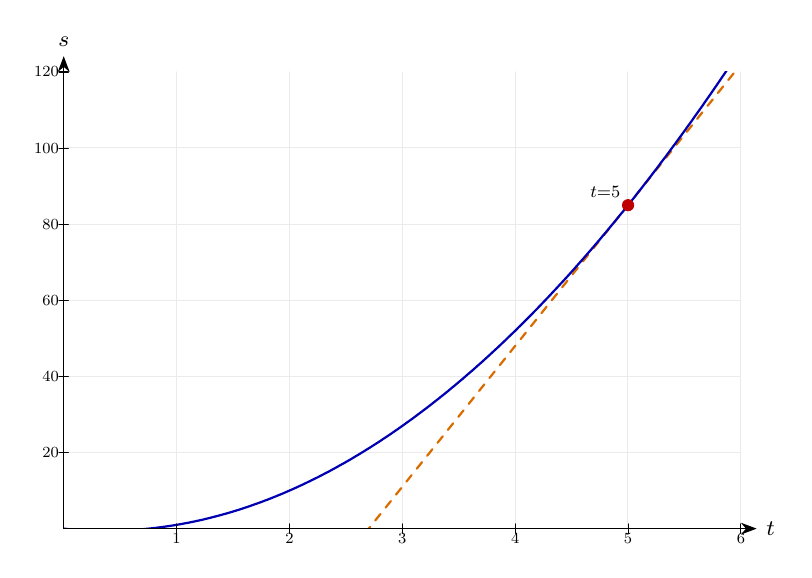
\begin{tikzpicture}[>={Stealth[length=2mm]},font=\footnotesize,line cap=round,line join=round]
\begin{scope}
\clip (0,0) rectangle (8.6,5.8);
\draw[gray!16] (0,0) grid[xstep=1.433,ystep=0.967] (8.6,5.8);
\draw[orange!85!black,thick,dashed] (0,-4.833) -- (8.6,5.897);
\draw[blue!70!black,thick] (0,0) -- (0.031,-0.003) -- (0.061,-0.006) -- (0.092,-0.009) -- (0.123,-0.011) -- (0.154,-0.013) -- (0.184,-0.015) -- (0.215,-0.017) -- (0.246,-0.019) -- (0.276,-0.021) -- (0.307,-0.022) -- (0.338,-0.023) -- (0.369,-0.025) -- (0.399,-0.025) -- (0.43,-0.026) -- (0.461,-0.027) -- (0.491,-0.027) -- (0.522,-0.027) -- (0.553,-0.027) -- (0.584,-0.027) -- (0.614,-0.027) -- (0.645,-0.026) -- (0.676,-0.025) -- (0.706,-0.025) -- (0.737,-0.023) -- (0.768,-0.022) -- (0.799,-0.021) -- (0.829,-0.019) -- (0.86,-0.017) -- (0.891,-0.015) -- (0.921,-0.013) -- (0.952,-0.011) -- (0.983,-0.009) -- (1.014,-0.006) -- (1.044,-0.003) -- (1.075,0) -- (1.106,0.003) -- (1.136,0.007) -- (1.167,0.01) -- (1.198,0.014) -- (1.229,0.018) -- (1.259,0.022) -- (1.29,0.026) -- (1.321,0.031) -- (1.351,0.035) -- (1.382,0.04) -- (1.413,0.045) -- (1.444,0.05) -- (1.474,0.055) -- (1.505,0.061) -- (1.536,0.067) -- (1.566,0.072) -- (1.597,0.078) -- (1.628,0.085) -- (1.659,0.091) -- (1.689,0.098) -- (1.72,0.104) -- (1.751,0.111) -- (1.781,0.118) -- (1.812,0.126) -- (1.843,0.133) -- (1.874,0.141) -- (1.904,0.149) -- (1.935,0.157) -- (1.966,0.165) -- (1.996,0.173) -- (2.027,0.182) -- (2.058,0.19) -- (2.089,0.199) -- (2.119,0.208) -- (2.15,0.217) -- (2.181,0.227) -- (2.211,0.236) -- (2.242,0.246) -- (2.273,0.256) -- (2.304,0.266) -- (2.334,0.277) -- (2.365,0.287) -- (2.396,0.298) -- (2.426,0.309) -- (2.457,0.32) -- (2.488,0.331) -- (2.519,0.342) -- (2.549,0.354) -- (2.58,0.365) -- (2.611,0.377) -- (2.641,0.389) -- (2.672,0.402) -- (2.703,0.414) -- (2.734,0.427) -- (2.764,0.439) -- (2.795,0.452) -- (2.826,0.466) -- (2.856,0.479) -- (2.887,0.492) -- (2.918,0.506) -- (2.949,0.52) -- (2.979,0.534) -- (3.01,0.548) -- (3.041,0.562) -- (3.071,0.577) -- (3.102,0.592) -- (3.133,0.607) -- (3.164,0.622) -- (3.194,0.637) -- (3.225,0.652) -- (3.256,0.668) -- (3.286,0.684) -- (3.317,0.7) -- (3.348,0.716) -- (3.379,0.732) -- (3.409,0.749) -- (3.44,0.766) -- (3.471,0.782) -- (3.501,0.8) -- (3.532,0.817) -- (3.563,0.834) -- (3.594,0.852) -- (3.624,0.869) -- (3.655,0.887) -- (3.686,0.906) -- (3.716,0.924) -- (3.747,0.942) -- (3.778,0.961) -- (3.809,0.98) -- (3.839,0.999) -- (3.87,1.018) -- (3.901,1.037) -- (3.931,1.057) -- (3.962,1.076) -- (3.993,1.096) -- (4.024,1.116) -- (4.054,1.137) -- (4.085,1.157) -- (4.116,1.178) -- (4.146,1.198) -- (4.177,1.219) -- (4.208,1.241) -- (4.239,1.262) -- (4.269,1.283) -- (4.3,1.305) -- (4.331,1.327) -- (4.361,1.349) -- (4.392,1.371) -- (4.423,1.393) -- (4.454,1.416) -- (4.484,1.439) -- (4.515,1.462) -- (4.546,1.485) -- (4.576,1.508) -- (4.607,1.531) -- (4.638,1.555) -- (4.669,1.579) -- (4.699,1.603) -- (4.73,1.627) -- (4.761,1.651) -- (4.791,1.676) -- (4.822,1.7) -- (4.853,1.725) -- (4.884,1.75) -- (4.914,1.776) -- (4.945,1.801) -- (4.976,1.826) -- (5.006,1.852) -- (5.037,1.878) -- (5.068,1.904) -- (5.099,1.931) -- (5.129,1.957) -- (5.16,1.984) -- (5.191,2.01) -- (5.221,2.037) -- (5.252,2.065) -- (5.283,2.092) -- (5.314,2.119) -- (5.344,2.147) -- (5.375,2.175) -- (5.406,2.203) -- (5.436,2.231) -- (5.467,2.26) -- (5.498,2.288) -- (5.529,2.317) -- (5.559,2.346) -- (5.59,2.375) -- (5.621,2.404) -- (5.651,2.434) -- (5.682,2.464) -- (5.713,2.493) -- (5.744,2.523) -- (5.774,2.554) -- (5.805,2.584) -- (5.836,2.614) -- (5.866,2.645) -- (5.897,2.676) -- (5.928,2.707) -- (5.959,2.738) -- (5.989,2.77) -- (6.02,2.801) -- (6.051,2.833) -- (6.081,2.865) -- (6.112,2.897) -- (6.143,2.93) -- (6.174,2.962) -- (6.204,2.995) -- (6.235,3.028) -- (6.266,3.061) -- (6.296,3.094) -- (6.327,3.127) -- (6.358,3.161) -- (6.389,3.194) -- (6.419,3.228) -- (6.45,3.262) -- (6.481,3.297) -- (6.511,3.331) -- (6.542,3.366) -- (6.573,3.401) -- (6.604,3.436) -- (6.634,3.471) -- (6.665,3.506) -- (6.696,3.542) -- (6.726,3.577) -- (6.757,3.613) -- (6.788,3.649) -- (6.819,3.685) -- (6.849,3.722) -- (6.88,3.758) -- (6.911,3.795) -- (6.941,3.832) -- (6.972,3.869) -- (7.003,3.906) -- (7.034,3.944) -- (7.064,3.982) -- (7.095,4.019) -- (7.126,4.057) -- (7.156,4.096) -- (7.187,4.134) -- (7.218,4.172) -- (7.249,4.211) -- (7.279,4.25) -- (7.31,4.289) -- (7.341,4.328) -- (7.371,4.368) -- (7.402,4.407) -- (7.433,4.447) -- (7.464,4.487) -- (7.494,4.527) -- (7.525,4.567) -- (7.556,4.608) -- (7.586,4.649) -- (7.617,4.689) -- (7.648,4.73) -- (7.679,4.772) -- (7.709,4.813) -- (7.74,4.855) -- (7.771,4.896) -- (7.801,4.938) -- (7.832,4.98) -- (7.863,5.023) -- (7.894,5.065) -- (7.924,5.108) -- (7.955,5.15) -- (7.986,5.193) -- (8.016,5.237) -- (8.047,5.28) -- (8.078,5.323) -- (8.109,5.367) -- (8.139,5.411) -- (8.17,5.455) -- (8.201,5.499) -- (8.231,5.543) -- (8.262,5.588) -- (8.293,5.633) -- (8.324,5.678) -- (8.354,5.723) -- (8.385,5.768) -- (8.416,5.814) -- (8.446,5.859) -- (8.477,5.905) -- (8.508,5.951) -- (8.539,5.997) -- (8.569,6.043) -- (8.6,6.09);
\end{scope}
\draw[->] (0,0) -- (8.8,0) node[right]{$t$};
\draw[->] (0,0) -- (0,6) node[above]{$s$};
\draw (1.433,-0.06) -- (1.433,0.06) node[below=1pt,scale=0.7]{$1$};
\draw (2.867,-0.06) -- (2.867,0.06) node[below=1pt,scale=0.7]{$2$};
\draw (4.3,-0.06) -- (4.3,0.06) node[below=1pt,scale=0.7]{$3$};
\draw (5.733,-0.06) -- (5.733,0.06) node[below=1pt,scale=0.7]{$4$};
\draw (7.167,-0.06) -- (7.167,0.06) node[below=1pt,scale=0.7]{$5$};
\draw (8.6,-0.06) -- (8.6,0.06) node[below=1pt,scale=0.7]{$6$};
\draw (-0.06,0.967) -- (0.06,0.967) node[left=1pt,scale=0.7]{$20$};
\draw (-0.06,1.933) -- (0.06,1.933) node[left=1pt,scale=0.7]{$40$};
\draw (-0.06,2.9) -- (0.06,2.9) node[left=1pt,scale=0.7]{$60$};
\draw (-0.06,3.867) -- (0.06,3.867) node[left=1pt,scale=0.7]{$80$};
\draw (-0.06,4.833) -- (0.06,4.833) node[left=1pt,scale=0.7]{$100$};
\draw (-0.06,5.8) -- (0.06,5.8) node[left=1pt,scale=0.7]{$120$};
\fill[red!75!black] (7.167,4.108) circle (2.2pt);
\node[above left,scale=0.78] at (7.167,4.108) {$t{=}5$};
\end{tikzpicture}
}
\end{center}
\small The model plotted against its variable, with the key point(s) marked and the tangent (dashed) showing the instantaneous rate.\normalsize

\medskip\hrule

\section*{Real-Life Problems 02\quad\small\texttt{(d5-002)}}
\addcontentsline{toc}{section}{Real-Life Problems 02 (d5-002)}
\textit{Difficulty: Foundation \quad\textbar\quad Marks: 4}

\question{A particle's displacement is \( s = t^3 - 6t^2 + 5 \) metres after \( t \) seconds. (a) Find the velocity function. (b) Find the acceleration function. (c) Find the acceleration when \( t = 4 \) seconds.}

\textbf{Worked solution.}

\textit{Step 1: (a) Differentiate \( s \) to get velocity.}
\[\begin{gathered}
v = \frac{\mathrm{d}s}{\mathrm{d}t} = 3t^2 - 12t
\end{gathered}\]
Power rule applied term by term.

\textit{Step 2: (b) Differentiate \( v \) to get acceleration.}
\[\begin{gathered}
a = \frac{\mathrm{d}v}{\mathrm{d}t} = \frac{\mathrm{d}^2s}{\mathrm{d}t^2} = 6t - 12
\end{gathered}\]
Acceleration is the rate of change of velocity.

\textit{Step 3: (c) Substitute \( t = 4 \).}
\[\begin{gathered}
a = 6(4) - 12 = 24 - 12 = 12 \text{ ms}^{-2}
\end{gathered}\]
Replace \( t \) with 4.

\begin{answerbox}
\textbf{Final answer:}\quad (a) \(\displaystyle  v = 3t^2 - 12t \) \\[3pt]  (b) \(\displaystyle  a = 6t - 12 \) \\[3pt]  (c) \(\displaystyle  a = 12 \text{ ms}^{-2} \)
\end{answerbox}
\textbf{Diagram.}

\begin{center}
\resizebox{\ifdim\width>\linewidth \linewidth\else \width\fi}{!}{%
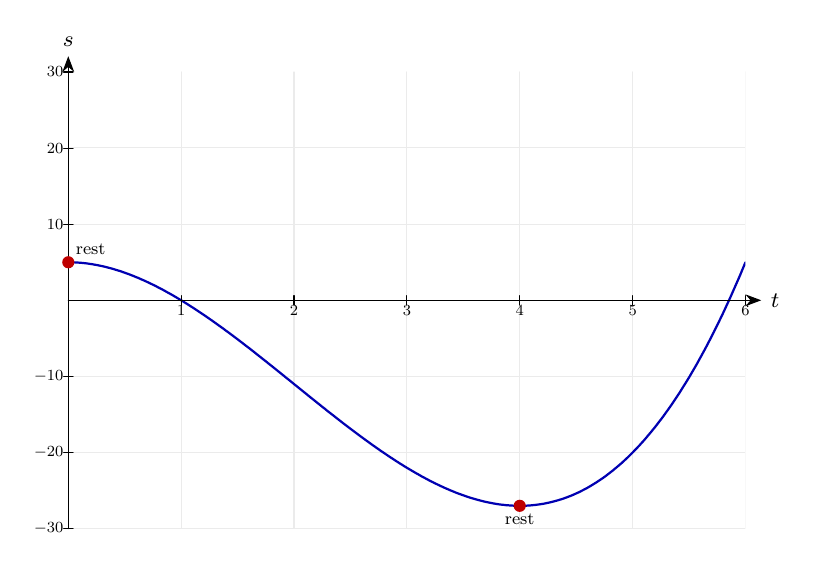
\begin{tikzpicture}[>={Stealth[length=2mm]},font=\footnotesize,line cap=round,line join=round]
\begin{scope}
\clip (0,0) rectangle (8.6,5.8);
\draw[gray!16] (0,0) grid[xstep=1.433,ystep=0.967] (8.6,5.8);
\draw[blue!70!black,thick] (0,3.383) -- (0.031,3.383) -- (0.061,3.382) -- (0.092,3.381) -- (0.123,3.379) -- (0.154,3.377) -- (0.184,3.374) -- (0.215,3.371) -- (0.246,3.367) -- (0.276,3.362) -- (0.307,3.358) -- (0.338,3.352) -- (0.369,3.347) -- (0.399,3.34) -- (0.43,3.334) -- (0.461,3.327) -- (0.491,3.319) -- (0.522,3.311) -- (0.553,3.303) -- (0.584,3.294) -- (0.614,3.284) -- (0.645,3.275) -- (0.676,3.265) -- (0.706,3.254) -- (0.737,3.243) -- (0.768,3.232) -- (0.799,3.22) -- (0.829,3.208) -- (0.86,3.195) -- (0.891,3.183) -- (0.921,3.169) -- (0.952,3.156) -- (0.983,3.142) -- (1.014,3.127) -- (1.044,3.113) -- (1.075,3.098) -- (1.106,3.083) -- (1.136,3.067) -- (1.167,3.051) -- (1.198,3.035) -- (1.229,3.018) -- (1.259,3.001) -- (1.29,2.984) -- (1.321,2.967) -- (1.351,2.949) -- (1.382,2.931) -- (1.413,2.912) -- (1.444,2.894) -- (1.474,2.875) -- (1.505,2.856) -- (1.536,2.836) -- (1.566,2.817) -- (1.597,2.797) -- (1.628,2.777) -- (1.659,2.756) -- (1.689,2.736) -- (1.72,2.715) -- (1.751,2.694) -- (1.781,2.673) -- (1.812,2.652) -- (1.843,2.63) -- (1.874,2.608) -- (1.904,2.586) -- (1.935,2.564) -- (1.966,2.542) -- (1.996,2.519) -- (2.027,2.497) -- (2.058,2.474) -- (2.089,2.451) -- (2.119,2.428) -- (2.15,2.405) -- (2.181,2.381) -- (2.211,2.358) -- (2.242,2.334) -- (2.273,2.31) -- (2.304,2.287) -- (2.334,2.263) -- (2.365,2.239) -- (2.396,2.214) -- (2.426,2.19) -- (2.457,2.166) -- (2.488,2.141) -- (2.519,2.117) -- (2.549,2.092) -- (2.58,2.068) -- (2.611,2.043) -- (2.641,2.019) -- (2.672,1.994) -- (2.703,1.969) -- (2.734,1.944) -- (2.764,1.919) -- (2.795,1.895) -- (2.826,1.87) -- (2.856,1.845) -- (2.887,1.82) -- (2.918,1.795) -- (2.949,1.77) -- (2.979,1.746) -- (3.01,1.721) -- (3.041,1.696) -- (3.071,1.671) -- (3.102,1.647) -- (3.133,1.622) -- (3.164,1.597) -- (3.194,1.573) -- (3.225,1.548) -- (3.256,1.524) -- (3.286,1.499) -- (3.317,1.475) -- (3.348,1.451) -- (3.379,1.427) -- (3.409,1.403) -- (3.44,1.379) -- (3.471,1.355) -- (3.501,1.331) -- (3.532,1.308) -- (3.563,1.284) -- (3.594,1.261) -- (3.624,1.238) -- (3.655,1.215) -- (3.686,1.192) -- (3.716,1.169) -- (3.747,1.147) -- (3.778,1.124) -- (3.809,1.102) -- (3.839,1.08) -- (3.87,1.058) -- (3.901,1.036) -- (3.931,1.015) -- (3.962,0.993) -- (3.993,0.972) -- (4.024,0.951) -- (4.054,0.931) -- (4.085,0.91) -- (4.116,0.89) -- (4.146,0.87) -- (4.177,0.85) -- (4.208,0.83) -- (4.239,0.811) -- (4.269,0.792) -- (4.3,0.773) -- (4.331,0.755) -- (4.361,0.737) -- (4.392,0.719) -- (4.423,0.701) -- (4.454,0.684) -- (4.484,0.666) -- (4.515,0.65) -- (4.546,0.633) -- (4.576,0.617) -- (4.607,0.601) -- (4.638,0.586) -- (4.669,0.57) -- (4.699,0.556) -- (4.73,0.541) -- (4.761,0.527) -- (4.791,0.513) -- (4.822,0.5) -- (4.853,0.486) -- (4.884,0.474) -- (4.914,0.461) -- (4.945,0.449) -- (4.976,0.438) -- (5.006,0.427) -- (5.037,0.416) -- (5.068,0.405) -- (5.099,0.395) -- (5.129,0.386) -- (5.16,0.377) -- (5.191,0.368) -- (5.221,0.36) -- (5.252,0.352) -- (5.283,0.344) -- (5.314,0.337) -- (5.344,0.331) -- (5.375,0.325) -- (5.406,0.319) -- (5.436,0.314) -- (5.467,0.309) -- (5.498,0.305) -- (5.529,0.302) -- (5.559,0.298) -- (5.59,0.296) -- (5.621,0.294) -- (5.651,0.292) -- (5.682,0.291) -- (5.713,0.29) -- (5.744,0.29) -- (5.774,0.29) -- (5.805,0.291) -- (5.836,0.293) -- (5.866,0.295) -- (5.897,0.298) -- (5.928,0.301) -- (5.959,0.305) -- (5.989,0.309) -- (6.02,0.314) -- (6.051,0.319) -- (6.081,0.326) -- (6.112,0.332) -- (6.143,0.34) -- (6.174,0.348) -- (6.204,0.356) -- (6.235,0.365) -- (6.266,0.375) -- (6.296,0.385) -- (6.327,0.396) -- (6.358,0.408) -- (6.389,0.42) -- (6.419,0.433) -- (6.45,0.447) -- (6.481,0.461) -- (6.511,0.476) -- (6.542,0.492) -- (6.573,0.508) -- (6.604,0.525) -- (6.634,0.543) -- (6.665,0.562) -- (6.696,0.581) -- (6.726,0.601) -- (6.757,0.621) -- (6.788,0.642) -- (6.819,0.664) -- (6.849,0.687) -- (6.88,0.711) -- (6.911,0.735) -- (6.941,0.76) -- (6.972,0.786) -- (7.003,0.812) -- (7.034,0.839) -- (7.064,0.867) -- (7.095,0.896) -- (7.126,0.926) -- (7.156,0.956) -- (7.187,0.988) -- (7.218,1.02) -- (7.249,1.052) -- (7.279,1.086) -- (7.31,1.12) -- (7.341,1.156) -- (7.371,1.192) -- (7.402,1.229) -- (7.433,1.267) -- (7.464,1.305) -- (7.494,1.345) -- (7.525,1.385) -- (7.556,1.426) -- (7.586,1.468) -- (7.617,1.511) -- (7.648,1.555) -- (7.679,1.6) -- (7.709,1.646) -- (7.74,1.692) -- (7.771,1.739) -- (7.801,1.788) -- (7.832,1.837) -- (7.863,1.887) -- (7.894,1.938) -- (7.924,1.99) -- (7.955,2.043) -- (7.986,2.097) -- (8.016,2.152) -- (8.047,2.208) -- (8.078,2.265) -- (8.109,2.323) -- (8.139,2.381) -- (8.17,2.441) -- (8.201,2.502) -- (8.231,2.564) -- (8.262,2.626) -- (8.293,2.69) -- (8.324,2.755) -- (8.354,2.82) -- (8.385,2.887) -- (8.416,2.955) -- (8.446,3.024) -- (8.477,3.094) -- (8.508,3.164) -- (8.539,3.236) -- (8.569,3.309) -- (8.6,3.383);
\end{scope}
\draw[->] (0,2.9) -- (8.8,2.9) node[right]{$t$};
\draw[->] (0,0) -- (0,6) node[above]{$s$};
\draw (1.433,2.84) -- (1.433,2.96) node[below=1pt,scale=0.7]{$1$};
\draw (2.867,2.84) -- (2.867,2.96) node[below=1pt,scale=0.7]{$2$};
\draw (4.3,2.84) -- (4.3,2.96) node[below=1pt,scale=0.7]{$3$};
\draw (5.733,2.84) -- (5.733,2.96) node[below=1pt,scale=0.7]{$4$};
\draw (7.167,2.84) -- (7.167,2.96) node[below=1pt,scale=0.7]{$5$};
\draw (8.6,2.84) -- (8.6,2.96) node[below=1pt,scale=0.7]{$6$};
\draw (-0.06,0) -- (0.06,0) node[left=1pt,scale=0.7]{$-30$};
\draw (-0.06,0.967) -- (0.06,0.967) node[left=1pt,scale=0.7]{$-20$};
\draw (-0.06,1.933) -- (0.06,1.933) node[left=1pt,scale=0.7]{$-10$};
\draw (-0.06,3.867) -- (0.06,3.867) node[left=1pt,scale=0.7]{$10$};
\draw (-0.06,4.833) -- (0.06,4.833) node[left=1pt,scale=0.7]{$20$};
\draw (-0.06,5.8) -- (0.06,5.8) node[left=1pt,scale=0.7]{$30$};
\fill[red!75!black] (0,3.383) circle (2.2pt);
\node[above right,scale=0.78] at (0,3.383) {rest};
\fill[red!75!black] (5.733,0.29) circle (2.2pt);
\node[below,scale=0.78] at (5.733,0.29) {rest};
\end{tikzpicture}
}
\end{center}
\small The model plotted against its variable, with the key point(s) marked.\normalsize

\medskip\hrule

\section*{Real-Life Problems 03\quad\small\texttt{(d5-003)}}
\addcontentsline{toc}{section}{Real-Life Problems 03 (d5-003)}
\textit{Difficulty: Foundation \quad\textbar\quad Marks: 4}

\question{A stone is thrown upwards. Its height \( h \) metres above the ground after \( t \) seconds is \( h = 20t - 5t^2 \). (a) Find the velocity of the stone after \( t \) seconds. (b) Find the time at which the stone is momentarily stationary (at its maximum height). (c) Find the maximum height reached.}

\textbf{Worked solution.}

\textit{Step 1: (a) Differentiate \( h \) with respect to \( t \).}
\[\begin{gathered}
v = \frac{\mathrm{d}h}{\mathrm{d}t} = 20 - 10t
\end{gathered}\]
Velocity is the derivative of displacement (height).

\textit{Step 2: (b) At maximum height the velocity is zero.}
\[\begin{gathered}
20 - 10t = 0 \implies t = 2 \text{ s}
\end{gathered}\]
Set \( v = 0 \) and solve for \( t \).

\textit{Step 3: (c) Substitute \( t = 2 \) into \( h \).}
\[\begin{gathered}
h = 20(2) - 5(4) = 40 - 20 = 20 \text{ m}
\end{gathered}\]
The maximum height occurs at \( t = 2 \).

\begin{answerbox}
\textbf{Final answer:}\quad (a) \(\displaystyle  v = 20 - 10t \) \\[3pt]  (b) \(\displaystyle  t = 2 \) s \\[3pt]  (c) Maximum height \(\displaystyle  = 20 \) m
\end{answerbox}
\textbf{Diagram.}

\begin{center}
\resizebox{\ifdim\width>\linewidth \linewidth\else \width\fi}{!}{%
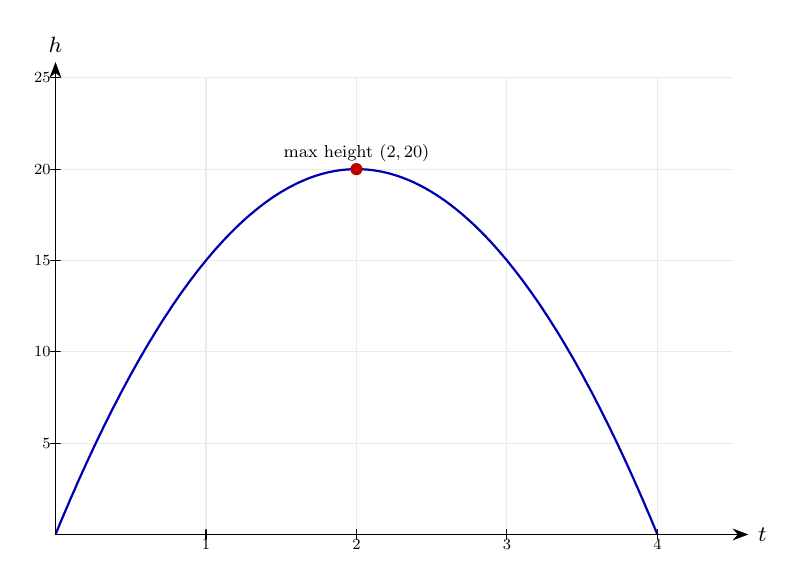
\begin{tikzpicture}[>={Stealth[length=2mm]},font=\footnotesize,line cap=round,line join=round]
\begin{scope}
\clip (0,0) rectangle (8.6,5.8);
\draw[gray!16] (0,0) grid[xstep=1.911,ystep=1.16] (8.6,5.8);
\draw[blue!70!black,thick] (0,0) -- (0.031,0.074) -- (0.061,0.148) -- (0.092,0.221) -- (0.123,0.293) -- (0.154,0.365) -- (0.184,0.437) -- (0.215,0.507) -- (0.246,0.577) -- (0.276,0.647) -- (0.307,0.716) -- (0.338,0.784) -- (0.369,0.852) -- (0.399,0.919) -- (0.43,0.985) -- (0.461,1.051) -- (0.491,1.116) -- (0.522,1.181) -- (0.553,1.245) -- (0.584,1.309) -- (0.614,1.372) -- (0.645,1.434) -- (0.676,1.496) -- (0.706,1.557) -- (0.737,1.617) -- (0.768,1.677) -- (0.799,1.736) -- (0.829,1.795) -- (0.86,1.853) -- (0.891,1.911) -- (0.921,1.967) -- (0.952,2.024) -- (0.983,2.079) -- (1.014,2.135) -- (1.044,2.189) -- (1.075,2.243) -- (1.106,2.296) -- (1.136,2.349) -- (1.167,2.401) -- (1.198,2.453) -- (1.229,2.503) -- (1.259,2.554) -- (1.29,2.603) -- (1.321,2.653) -- (1.351,2.701) -- (1.382,2.749) -- (1.413,2.796) -- (1.444,2.843) -- (1.474,2.889) -- (1.505,2.935) -- (1.536,2.98) -- (1.566,3.024) -- (1.597,3.068) -- (1.628,3.111) -- (1.659,3.153) -- (1.689,3.195) -- (1.72,3.236) -- (1.751,3.277) -- (1.781,3.317) -- (1.812,3.357) -- (1.843,3.396) -- (1.874,3.434) -- (1.904,3.472) -- (1.935,3.509) -- (1.966,3.545) -- (1.996,3.581) -- (2.027,3.617) -- (2.058,3.651) -- (2.089,3.685) -- (2.119,3.719) -- (2.15,3.752) -- (2.181,3.784) -- (2.211,3.816) -- (2.242,3.847) -- (2.273,3.878) -- (2.304,3.908) -- (2.334,3.937) -- (2.365,3.966) -- (2.396,3.994) -- (2.426,4.021) -- (2.457,4.048) -- (2.488,4.074) -- (2.519,4.1) -- (2.549,4.125) -- (2.58,4.15) -- (2.611,4.174) -- (2.641,4.197) -- (2.672,4.22) -- (2.703,4.242) -- (2.734,4.264) -- (2.764,4.285) -- (2.795,4.305) -- (2.826,4.325) -- (2.856,4.344) -- (2.887,4.362) -- (2.918,4.38) -- (2.949,4.398) -- (2.979,4.414) -- (3.01,4.43) -- (3.041,4.446) -- (3.071,4.461) -- (3.102,4.475) -- (3.133,4.489) -- (3.164,4.502) -- (3.194,4.515) -- (3.225,4.527) -- (3.256,4.538) -- (3.286,4.549) -- (3.317,4.559) -- (3.348,4.569) -- (3.379,4.577) -- (3.409,4.586) -- (3.44,4.594) -- (3.471,4.601) -- (3.501,4.607) -- (3.532,4.613) -- (3.563,4.619) -- (3.594,4.623) -- (3.624,4.628) -- (3.655,4.631) -- (3.686,4.634) -- (3.716,4.636) -- (3.747,4.638) -- (3.778,4.639) -- (3.809,4.64) -- (3.839,4.64) -- (3.87,4.639) -- (3.901,4.638) -- (3.931,4.636) -- (3.962,4.634) -- (3.993,4.631) -- (4.024,4.627) -- (4.054,4.623) -- (4.085,4.618) -- (4.116,4.613) -- (4.146,4.607) -- (4.177,4.6) -- (4.208,4.593) -- (4.239,4.585) -- (4.269,4.577) -- (4.3,4.567) -- (4.331,4.558) -- (4.361,4.548) -- (4.392,4.537) -- (4.423,4.525) -- (4.454,4.513) -- (4.484,4.501) -- (4.515,4.488) -- (4.546,4.474) -- (4.576,4.459) -- (4.607,4.444) -- (4.638,4.429) -- (4.669,4.412) -- (4.699,4.396) -- (4.73,4.378) -- (4.761,4.36) -- (4.791,4.342) -- (4.822,4.322) -- (4.853,4.303) -- (4.884,4.282) -- (4.914,4.261) -- (4.945,4.24) -- (4.976,4.217) -- (5.006,4.195) -- (5.037,4.171) -- (5.068,4.147) -- (5.099,4.123) -- (5.129,4.097) -- (5.16,4.072) -- (5.191,4.045) -- (5.221,4.018) -- (5.252,3.991) -- (5.283,3.962) -- (5.314,3.934) -- (5.344,3.904) -- (5.375,3.874) -- (5.406,3.844) -- (5.436,3.812) -- (5.467,3.781) -- (5.498,3.748) -- (5.529,3.715) -- (5.559,3.682) -- (5.59,3.647) -- (5.621,3.613) -- (5.651,3.577) -- (5.682,3.541) -- (5.713,3.505) -- (5.744,3.468) -- (5.774,3.43) -- (5.805,3.391) -- (5.836,3.352) -- (5.866,3.313) -- (5.897,3.273) -- (5.928,3.232) -- (5.959,3.19) -- (5.989,3.148) -- (6.02,3.106) -- (6.051,3.063) -- (6.081,3.019) -- (6.112,2.975) -- (6.143,2.93) -- (6.174,2.884) -- (6.204,2.838) -- (6.235,2.791) -- (6.266,2.744) -- (6.296,2.696) -- (6.327,2.647) -- (6.358,2.598) -- (6.389,2.548) -- (6.419,2.498) -- (6.45,2.447) -- (6.481,2.395) -- (6.511,2.343) -- (6.542,2.29) -- (6.573,2.237) -- (6.604,2.183) -- (6.634,2.128) -- (6.665,2.073) -- (6.696,2.018) -- (6.726,1.961) -- (6.757,1.904) -- (6.788,1.847) -- (6.819,1.789) -- (6.849,1.73) -- (6.88,1.67) -- (6.911,1.61) -- (6.941,1.55) -- (6.972,1.489) -- (7.003,1.427) -- (7.034,1.365) -- (7.064,1.302) -- (7.095,1.238) -- (7.126,1.174) -- (7.156,1.109) -- (7.187,1.044) -- (7.218,0.978) -- (7.249,0.911) -- (7.279,0.844) -- (7.31,0.776) -- (7.341,0.708) -- (7.371,0.639) -- (7.402,0.57) -- (7.433,0.499) -- (7.464,0.429) -- (7.494,0.357) -- (7.525,0.285) -- (7.556,0.213) -- (7.586,0.14) -- (7.617,0.066) -- (7.648,-0.008) -- (7.679,-0.083) -- (7.709,-0.159) -- (7.74,-0.235) -- (7.771,-0.312) -- (7.801,-0.389) -- (7.832,-0.467) -- (7.863,-0.545) -- (7.894,-0.625) -- (7.924,-0.704) -- (7.955,-0.785) -- (7.986,-0.866) -- (8.016,-0.947) -- (8.047,-1.029) -- (8.078,-1.112) -- (8.109,-1.195) -- (8.139,-1.279) -- (8.17,-1.364) -- (8.201,-1.449) -- (8.231,-1.535) -- (8.262,-1.621) -- (8.293,-1.708) -- (8.324,-1.795) -- (8.354,-1.883) -- (8.385,-1.972) -- (8.416,-2.062) -- (8.446,-2.151) -- (8.477,-2.242) -- (8.508,-2.333) -- (8.539,-2.425) -- (8.569,-2.517) -- (8.6,-2.61);
\end{scope}
\draw[->] (0,0) -- (8.8,0) node[right]{$t$};
\draw[->] (0,0) -- (0,6) node[above]{$h$};
\draw (1.911,-0.06) -- (1.911,0.06) node[below=1pt,scale=0.7]{$1$};
\draw (3.822,-0.06) -- (3.822,0.06) node[below=1pt,scale=0.7]{$2$};
\draw (5.733,-0.06) -- (5.733,0.06) node[below=1pt,scale=0.7]{$3$};
\draw (7.644,-0.06) -- (7.644,0.06) node[below=1pt,scale=0.7]{$4$};
\draw (-0.06,1.16) -- (0.06,1.16) node[left=1pt,scale=0.7]{$5$};
\draw (-0.06,2.32) -- (0.06,2.32) node[left=1pt,scale=0.7]{$10$};
\draw (-0.06,3.48) -- (0.06,3.48) node[left=1pt,scale=0.7]{$15$};
\draw (-0.06,4.64) -- (0.06,4.64) node[left=1pt,scale=0.7]{$20$};
\draw (-0.06,5.8) -- (0.06,5.8) node[left=1pt,scale=0.7]{$25$};
\fill[red!75!black] (3.822,4.64) circle (2.2pt);
\node[above,scale=0.78] at (3.822,4.64) {max height $(2,20)$};
\end{tikzpicture}
}
\end{center}
\small The model plotted against its variable, with the key point(s) marked.\normalsize

\medskip\hrule

\section*{Real-Life Problems 04\quad\small\texttt{(d5-004)}}
\addcontentsline{toc}{section}{Real-Life Problems 04 (d5-004)}
\textit{Difficulty: Foundation \quad\textbar\quad Marks: 4}

\question{A particle moves along a straight line. Its displacement \( s \) metres after \( t \) seconds is \( s = t^3 - 9t^2 + 24t \) for \( t \geq 0 \). (a) Find the velocity function \( v(t) \). (b) Find the values of \( t \) at which the particle is momentarily at rest.}

\textbf{Worked solution.}

\textit{Step 1: (a) Differentiate.}
\[\begin{gathered}
v = \frac{\mathrm{d}s}{\mathrm{d}t} = 3t^2 - 18t + 24
\end{gathered}\]
Power rule.

\textit{Step 2: (b) Set \( v = 0 \).}
\[\begin{gathered}
3t^2 - 18t + 24 = 0 \implies t^2 - 6t + 8 = 0 \implies (t-2)(t-4) = 0
\end{gathered}\]
Divide by 3 and factorise.

\textit{Step 3: Solve.}
\[\begin{gathered}
t = 2 \text{ s or } t = 4 \text{ s}
\end{gathered}\]
Both values are non-negative, so both are valid.

\begin{answerbox}
\textbf{Final answer:}\quad (a) \(\displaystyle  v = 3t^2 - 18t + 24 \) \\[3pt]  (b) \(\displaystyle  t = 2 \) s and \(\displaystyle  t = 4 \) s
\end{answerbox}
\textbf{Diagram.}

\begin{center}
\resizebox{\ifdim\width>\linewidth \linewidth\else \width\fi}{!}{%
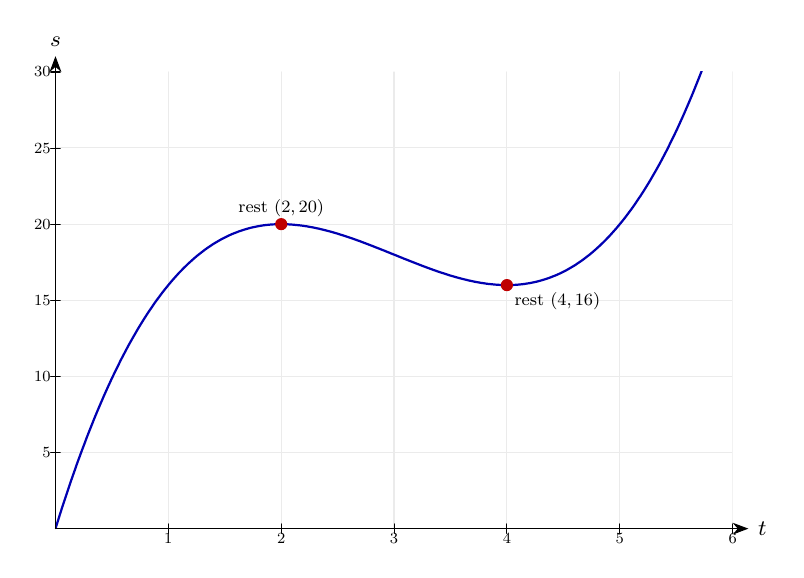
\begin{tikzpicture}[>={Stealth[length=2mm]},font=\footnotesize,line cap=round,line join=round]
\begin{scope}
\clip (0,0) rectangle (8.6,5.8);
\draw[gray!16] (0,0) grid[xstep=1.433,ystep=0.967] (8.6,5.8);
\draw[blue!70!black,thick] (0,0) -- (0.031,0.099) -- (0.061,0.196) -- (0.092,0.291) -- (0.123,0.385) -- (0.154,0.477) -- (0.184,0.568) -- (0.215,0.658) -- (0.246,0.745) -- (0.276,0.832) -- (0.307,0.916) -- (0.338,1) -- (0.369,1.081) -- (0.399,1.162) -- (0.43,1.241) -- (0.461,1.318) -- (0.491,1.394) -- (0.522,1.469) -- (0.553,1.542) -- (0.584,1.614) -- (0.614,1.684) -- (0.645,1.753) -- (0.676,1.821) -- (0.706,1.887) -- (0.737,1.952) -- (0.768,2.016) -- (0.799,2.078) -- (0.829,2.14) -- (0.86,2.199) -- (0.891,2.258) -- (0.921,2.315) -- (0.952,2.371) -- (0.983,2.426) -- (1.014,2.479) -- (1.044,2.532) -- (1.075,2.583) -- (1.106,2.633) -- (1.136,2.681) -- (1.167,2.729) -- (1.198,2.775) -- (1.229,2.821) -- (1.259,2.865) -- (1.29,2.908) -- (1.321,2.949) -- (1.351,2.99) -- (1.382,3.03) -- (1.413,3.068) -- (1.444,3.106) -- (1.474,3.142) -- (1.505,3.177) -- (1.536,3.212) -- (1.566,3.245) -- (1.597,3.277) -- (1.628,3.309) -- (1.659,3.339) -- (1.689,3.368) -- (1.72,3.396) -- (1.751,3.424) -- (1.781,3.45) -- (1.812,3.476) -- (1.843,3.5) -- (1.874,3.524) -- (1.904,3.547) -- (1.935,3.569) -- (1.966,3.589) -- (1.996,3.61) -- (2.027,3.629) -- (2.058,3.647) -- (2.089,3.665) -- (2.119,3.682) -- (2.15,3.697) -- (2.181,3.713) -- (2.211,3.727) -- (2.242,3.741) -- (2.273,3.753) -- (2.304,3.765) -- (2.334,3.777) -- (2.365,3.787) -- (2.396,3.797) -- (2.426,3.806) -- (2.457,3.815) -- (2.488,3.823) -- (2.519,3.83) -- (2.549,3.836) -- (2.58,3.842) -- (2.611,3.847) -- (2.641,3.852) -- (2.672,3.856) -- (2.703,3.859) -- (2.734,3.862) -- (2.764,3.864) -- (2.795,3.865) -- (2.826,3.866) -- (2.856,3.867) -- (2.887,3.867) -- (2.918,3.866) -- (2.949,3.865) -- (2.979,3.863) -- (3.01,3.861) -- (3.041,3.858) -- (3.071,3.855) -- (3.102,3.852) -- (3.133,3.848) -- (3.164,3.843) -- (3.194,3.839) -- (3.225,3.833) -- (3.256,3.828) -- (3.286,3.822) -- (3.317,3.815) -- (3.348,3.809) -- (3.379,3.801) -- (3.409,3.794) -- (3.44,3.786) -- (3.471,3.778) -- (3.501,3.77) -- (3.532,3.761) -- (3.563,3.752) -- (3.594,3.743) -- (3.624,3.733) -- (3.655,3.723) -- (3.686,3.713) -- (3.716,3.703) -- (3.747,3.693) -- (3.778,3.682) -- (3.809,3.671) -- (3.839,3.66) -- (3.87,3.649) -- (3.901,3.637) -- (3.931,3.626) -- (3.962,3.614) -- (3.993,3.602) -- (4.024,3.59) -- (4.054,3.578) -- (4.085,3.566) -- (4.116,3.554) -- (4.146,3.542) -- (4.177,3.53) -- (4.208,3.517) -- (4.239,3.505) -- (4.269,3.492) -- (4.3,3.48) -- (4.331,3.468) -- (4.361,3.455) -- (4.392,3.443) -- (4.423,3.43) -- (4.454,3.418) -- (4.484,3.406) -- (4.515,3.394) -- (4.546,3.382) -- (4.576,3.37) -- (4.607,3.358) -- (4.638,3.346) -- (4.669,3.334) -- (4.699,3.323) -- (4.73,3.311) -- (4.761,3.3) -- (4.791,3.289) -- (4.822,3.278) -- (4.853,3.267) -- (4.884,3.257) -- (4.914,3.247) -- (4.945,3.237) -- (4.976,3.227) -- (5.006,3.217) -- (5.037,3.208) -- (5.068,3.199) -- (5.099,3.19) -- (5.129,3.182) -- (5.16,3.174) -- (5.191,3.166) -- (5.221,3.159) -- (5.252,3.151) -- (5.283,3.145) -- (5.314,3.138) -- (5.344,3.132) -- (5.375,3.127) -- (5.406,3.121) -- (5.436,3.117) -- (5.467,3.112) -- (5.498,3.108) -- (5.529,3.105) -- (5.559,3.102) -- (5.59,3.099) -- (5.621,3.097) -- (5.651,3.095) -- (5.682,3.094) -- (5.713,3.093) -- (5.744,3.093) -- (5.774,3.094) -- (5.805,3.095) -- (5.836,3.096) -- (5.866,3.098) -- (5.897,3.101) -- (5.928,3.104) -- (5.959,3.108) -- (5.989,3.113) -- (6.02,3.118) -- (6.051,3.124) -- (6.081,3.13) -- (6.112,3.137) -- (6.143,3.145) -- (6.174,3.154) -- (6.204,3.163) -- (6.235,3.173) -- (6.266,3.183) -- (6.296,3.195) -- (6.327,3.207) -- (6.358,3.219) -- (6.389,3.233) -- (6.419,3.247) -- (6.45,3.262) -- (6.481,3.278) -- (6.511,3.295) -- (6.542,3.313) -- (6.573,3.331) -- (6.604,3.35) -- (6.634,3.371) -- (6.665,3.391) -- (6.696,3.413) -- (6.726,3.436) -- (6.757,3.46) -- (6.788,3.484) -- (6.819,3.51) -- (6.849,3.536) -- (6.88,3.564) -- (6.911,3.592) -- (6.941,3.621) -- (6.972,3.651) -- (7.003,3.683) -- (7.034,3.715) -- (7.064,3.748) -- (7.095,3.783) -- (7.126,3.818) -- (7.156,3.854) -- (7.187,3.892) -- (7.218,3.93) -- (7.249,3.97) -- (7.279,4.011) -- (7.31,4.052) -- (7.341,4.095) -- (7.371,4.139) -- (7.402,4.185) -- (7.433,4.231) -- (7.464,4.279) -- (7.494,4.327) -- (7.525,4.377) -- (7.556,4.428) -- (7.586,4.481) -- (7.617,4.534) -- (7.648,4.589) -- (7.679,4.645) -- (7.709,4.702) -- (7.74,4.761) -- (7.771,4.82) -- (7.801,4.882) -- (7.832,4.944) -- (7.863,5.008) -- (7.894,5.073) -- (7.924,5.139) -- (7.955,5.207) -- (7.986,5.276) -- (8.016,5.346) -- (8.047,5.418) -- (8.078,5.491) -- (8.109,5.566) -- (8.139,5.642) -- (8.17,5.719) -- (8.201,5.798) -- (8.231,5.879) -- (8.262,5.96) -- (8.293,6.044) -- (8.324,6.128) -- (8.354,6.215) -- (8.385,6.302) -- (8.416,6.392) -- (8.446,6.483) -- (8.477,6.575) -- (8.508,6.669) -- (8.539,6.764) -- (8.569,6.861) -- (8.6,6.96);
\end{scope}
\draw[->] (0,0) -- (8.8,0) node[right]{$t$};
\draw[->] (0,0) -- (0,6) node[above]{$s$};
\draw (1.433,-0.06) -- (1.433,0.06) node[below=1pt,scale=0.7]{$1$};
\draw (2.867,-0.06) -- (2.867,0.06) node[below=1pt,scale=0.7]{$2$};
\draw (4.3,-0.06) -- (4.3,0.06) node[below=1pt,scale=0.7]{$3$};
\draw (5.733,-0.06) -- (5.733,0.06) node[below=1pt,scale=0.7]{$4$};
\draw (7.167,-0.06) -- (7.167,0.06) node[below=1pt,scale=0.7]{$5$};
\draw (8.6,-0.06) -- (8.6,0.06) node[below=1pt,scale=0.7]{$6$};
\draw (-0.06,0.967) -- (0.06,0.967) node[left=1pt,scale=0.7]{$5$};
\draw (-0.06,1.933) -- (0.06,1.933) node[left=1pt,scale=0.7]{$10$};
\draw (-0.06,2.9) -- (0.06,2.9) node[left=1pt,scale=0.7]{$15$};
\draw (-0.06,3.867) -- (0.06,3.867) node[left=1pt,scale=0.7]{$20$};
\draw (-0.06,4.833) -- (0.06,4.833) node[left=1pt,scale=0.7]{$25$};
\draw (-0.06,5.8) -- (0.06,5.8) node[left=1pt,scale=0.7]{$30$};
\fill[red!75!black] (2.867,3.867) circle (2.2pt);
\node[above,scale=0.78] at (2.867,3.867) {rest $(2,20)$};
\fill[red!75!black] (5.733,3.093) circle (2.2pt);
\node[below right,scale=0.78] at (5.733,3.093) {rest $(4,16)$};
\end{tikzpicture}
}
\end{center}
\small The model plotted against its variable, with the key point(s) marked.\normalsize

\medskip\hrule

\section*{Real-Life Problems 05\quad\small\texttt{(d5-005)}}
\addcontentsline{toc}{section}{Real-Life Problems 05 (d5-005)}
\textit{Difficulty: Foundation \quad\textbar\quad Marks: 3}

\question{A motorbike starts from rest and travels along a straight road. After \( t \) seconds its displacement is \( s = 3t^2 \) metres. (a) Find the velocity after \( t \) seconds. (b) Find the velocity after 6 seconds. (c) Find the constant acceleration of the motorbike.}

\textbf{Worked solution.}

\textit{Step 1: (a) Differentiate \( s = 3t^2 \).}
\[\begin{gathered}
v = \frac{\mathrm{d}s}{\mathrm{d}t} = 6t
\end{gathered}\]
Power rule.

\textit{Step 2: (b) Substitute \( t = 6 \).}
\[\begin{gathered}
v = 6(6) = 36 \text{ ms}^{-1}
\end{gathered}\]
Replace \( t \) with 6.

\textit{Step 3: (c) Differentiate \( v = 6t \).}
\[\begin{gathered}
a = \frac{\mathrm{d}v}{\mathrm{d}t} = 6 \text{ ms}^{-2}
\end{gathered}\]
The acceleration is constant at \( 6 \text{ ms}^{-2} \).

\begin{answerbox}
\textbf{Final answer:}\quad (a) \(\displaystyle  v = 6t \) \\[3pt]  (b) \(\displaystyle  36 \text{ ms}^{-1} \) \\[3pt]  (c) \(\displaystyle  a = 6 \text{ ms}^{-2} \)
\end{answerbox}
\textbf{Diagram.}

\begin{center}
\resizebox{\ifdim\width>\linewidth \linewidth\else \width\fi}{!}{%
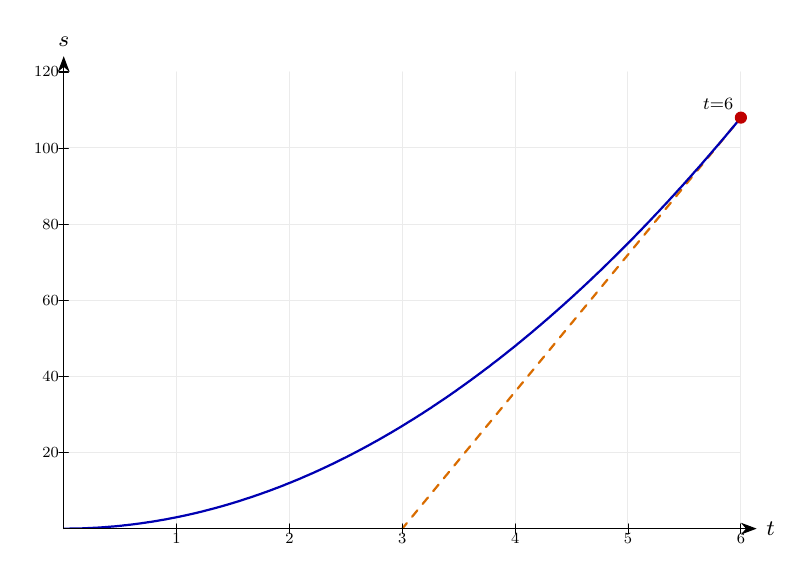
\begin{tikzpicture}[>={Stealth[length=2mm]},font=\footnotesize,line cap=round,line join=round]
\begin{scope}
\clip (0,0) rectangle (8.6,5.8);
\draw[gray!16] (0,0) grid[xstep=1.433,ystep=0.967] (8.6,5.8);
\draw[orange!85!black,thick,dashed] (0,-5.22) -- (8.6,5.22);
\draw[blue!70!black,thick] (0,0) -- (0.031,0) -- (0.061,0) -- (0.092,0.001) -- (0.123,0.001) -- (0.154,0.002) -- (0.184,0.002) -- (0.215,0.003) -- (0.246,0.004) -- (0.276,0.005) -- (0.307,0.007) -- (0.338,0.008) -- (0.369,0.01) -- (0.399,0.011) -- (0.43,0.013) -- (0.461,0.015) -- (0.491,0.017) -- (0.522,0.019) -- (0.553,0.022) -- (0.584,0.024) -- (0.614,0.027) -- (0.645,0.029) -- (0.676,0.032) -- (0.706,0.035) -- (0.737,0.038) -- (0.768,0.042) -- (0.799,0.045) -- (0.829,0.049) -- (0.86,0.052) -- (0.891,0.056) -- (0.921,0.06) -- (0.952,0.064) -- (0.983,0.068) -- (1.014,0.073) -- (1.044,0.077) -- (1.075,0.082) -- (1.106,0.086) -- (1.136,0.091) -- (1.167,0.096) -- (1.198,0.101) -- (1.229,0.107) -- (1.259,0.112) -- (1.29,0.117) -- (1.321,0.123) -- (1.351,0.129) -- (1.382,0.135) -- (1.413,0.141) -- (1.444,0.147) -- (1.474,0.153) -- (1.505,0.16) -- (1.536,0.166) -- (1.566,0.173) -- (1.597,0.18) -- (1.628,0.187) -- (1.659,0.194) -- (1.689,0.201) -- (1.72,0.209) -- (1.751,0.216) -- (1.781,0.224) -- (1.812,0.232) -- (1.843,0.24) -- (1.874,0.248) -- (1.904,0.256) -- (1.935,0.264) -- (1.966,0.273) -- (1.996,0.281) -- (2.027,0.29) -- (2.058,0.299) -- (2.089,0.308) -- (2.119,0.317) -- (2.15,0.326) -- (2.181,0.336) -- (2.211,0.345) -- (2.242,0.355) -- (2.273,0.365) -- (2.304,0.375) -- (2.334,0.385) -- (2.365,0.395) -- (2.396,0.405) -- (2.426,0.416) -- (2.457,0.426) -- (2.488,0.437) -- (2.519,0.448) -- (2.549,0.459) -- (2.58,0.47) -- (2.611,0.481) -- (2.641,0.492) -- (2.672,0.504) -- (2.703,0.516) -- (2.734,0.527) -- (2.764,0.539) -- (2.795,0.551) -- (2.826,0.564) -- (2.856,0.576) -- (2.887,0.588) -- (2.918,0.601) -- (2.949,0.614) -- (2.979,0.626) -- (3.01,0.639) -- (3.041,0.653) -- (3.071,0.666) -- (3.102,0.679) -- (3.133,0.693) -- (3.164,0.706) -- (3.194,0.72) -- (3.225,0.734) -- (3.256,0.748) -- (3.286,0.762) -- (3.317,0.777) -- (3.348,0.791) -- (3.379,0.806) -- (3.409,0.82) -- (3.44,0.835) -- (3.471,0.85) -- (3.501,0.865) -- (3.532,0.881) -- (3.563,0.896) -- (3.594,0.911) -- (3.624,0.927) -- (3.655,0.943) -- (3.686,0.959) -- (3.716,0.975) -- (3.747,0.991) -- (3.778,1.007) -- (3.809,1.024) -- (3.839,1.04) -- (3.87,1.057) -- (3.901,1.074) -- (3.931,1.091) -- (3.962,1.108) -- (3.993,1.125) -- (4.024,1.143) -- (4.054,1.16) -- (4.085,1.178) -- (4.116,1.196) -- (4.146,1.213) -- (4.177,1.231) -- (4.208,1.25) -- (4.239,1.268) -- (4.269,1.286) -- (4.3,1.305) -- (4.331,1.324) -- (4.361,1.343) -- (4.392,1.362) -- (4.423,1.381) -- (4.454,1.4) -- (4.484,1.419) -- (4.515,1.439) -- (4.546,1.458) -- (4.576,1.478) -- (4.607,1.498) -- (4.638,1.518) -- (4.669,1.538) -- (4.699,1.559) -- (4.73,1.579) -- (4.761,1.6) -- (4.791,1.62) -- (4.822,1.641) -- (4.853,1.662) -- (4.884,1.683) -- (4.914,1.704) -- (4.945,1.726) -- (4.976,1.747) -- (5.006,1.769) -- (5.037,1.791) -- (5.068,1.813) -- (5.099,1.835) -- (5.129,1.857) -- (5.16,1.879) -- (5.191,1.902) -- (5.221,1.924) -- (5.252,1.947) -- (5.283,1.97) -- (5.314,1.993) -- (5.344,2.016) -- (5.375,2.039) -- (5.406,2.062) -- (5.436,2.086) -- (5.467,2.11) -- (5.498,2.133) -- (5.529,2.157) -- (5.559,2.181) -- (5.59,2.205) -- (5.621,2.23) -- (5.651,2.254) -- (5.682,2.279) -- (5.713,2.303) -- (5.744,2.328) -- (5.774,2.353) -- (5.805,2.378) -- (5.836,2.404) -- (5.866,2.429) -- (5.897,2.454) -- (5.928,2.48) -- (5.959,2.506) -- (5.989,2.532) -- (6.02,2.558) -- (6.051,2.584) -- (6.081,2.61) -- (6.112,2.637) -- (6.143,2.663) -- (6.174,2.69) -- (6.204,2.717) -- (6.235,2.744) -- (6.266,2.771) -- (6.296,2.798) -- (6.327,2.825) -- (6.358,2.853) -- (6.389,2.881) -- (6.419,2.908) -- (6.45,2.936) -- (6.481,2.964) -- (6.511,2.992) -- (6.542,3.021) -- (6.573,3.049) -- (6.604,3.078) -- (6.634,3.106) -- (6.665,3.135) -- (6.696,3.164) -- (6.726,3.193) -- (6.757,3.223) -- (6.788,3.252) -- (6.819,3.281) -- (6.849,3.311) -- (6.88,3.341) -- (6.911,3.371) -- (6.941,3.401) -- (6.972,3.431) -- (7.003,3.461) -- (7.034,3.492) -- (7.064,3.522) -- (7.095,3.553) -- (7.126,3.584) -- (7.156,3.615) -- (7.187,3.646) -- (7.218,3.677) -- (7.249,3.708) -- (7.279,3.74) -- (7.31,3.771) -- (7.341,3.803) -- (7.371,3.835) -- (7.402,3.867) -- (7.433,3.899) -- (7.464,3.932) -- (7.494,3.964) -- (7.525,3.997) -- (7.556,4.029) -- (7.586,4.062) -- (7.617,4.095) -- (7.648,4.128) -- (7.679,4.161) -- (7.709,4.195) -- (7.74,4.228) -- (7.771,4.262) -- (7.801,4.296) -- (7.832,4.329) -- (7.863,4.363) -- (7.894,4.398) -- (7.924,4.432) -- (7.955,4.466) -- (7.986,4.501) -- (8.016,4.536) -- (8.047,4.57) -- (8.078,4.605) -- (8.109,4.64) -- (8.139,4.676) -- (8.17,4.711) -- (8.201,4.747) -- (8.231,4.782) -- (8.262,4.818) -- (8.293,4.854) -- (8.324,4.89) -- (8.354,4.926) -- (8.385,4.962) -- (8.416,4.999) -- (8.446,5.035) -- (8.477,5.072) -- (8.508,5.109) -- (8.539,5.146) -- (8.569,5.183) -- (8.6,5.22);
\end{scope}
\draw[->] (0,0) -- (8.8,0) node[right]{$t$};
\draw[->] (0,0) -- (0,6) node[above]{$s$};
\draw (1.433,-0.06) -- (1.433,0.06) node[below=1pt,scale=0.7]{$1$};
\draw (2.867,-0.06) -- (2.867,0.06) node[below=1pt,scale=0.7]{$2$};
\draw (4.3,-0.06) -- (4.3,0.06) node[below=1pt,scale=0.7]{$3$};
\draw (5.733,-0.06) -- (5.733,0.06) node[below=1pt,scale=0.7]{$4$};
\draw (7.167,-0.06) -- (7.167,0.06) node[below=1pt,scale=0.7]{$5$};
\draw (8.6,-0.06) -- (8.6,0.06) node[below=1pt,scale=0.7]{$6$};
\draw (-0.06,0.967) -- (0.06,0.967) node[left=1pt,scale=0.7]{$20$};
\draw (-0.06,1.933) -- (0.06,1.933) node[left=1pt,scale=0.7]{$40$};
\draw (-0.06,2.9) -- (0.06,2.9) node[left=1pt,scale=0.7]{$60$};
\draw (-0.06,3.867) -- (0.06,3.867) node[left=1pt,scale=0.7]{$80$};
\draw (-0.06,4.833) -- (0.06,4.833) node[left=1pt,scale=0.7]{$100$};
\draw (-0.06,5.8) -- (0.06,5.8) node[left=1pt,scale=0.7]{$120$};
\fill[red!75!black] (8.6,5.22) circle (2.2pt);
\node[above left,scale=0.78] at (8.6,5.22) {$t{=}6$};
\end{tikzpicture}
}
\end{center}
\small The model plotted against its variable, with the key point(s) marked and the tangent (dashed) showing the instantaneous rate.\normalsize

\medskip\hrule

\section*{Real-Life Problems 06\quad\small\texttt{(d5-006)}}
\addcontentsline{toc}{section}{Real-Life Problems 06 (d5-006)}
\textit{Difficulty: Foundation \quad\textbar\quad Marks: 5}

\question{A particle's displacement in metres is given by \( s = 2t^3 - 15t^2 + 36t \) for \( t \geq 0 \). (a) Find the velocity when \( t = 3 \). (b) Find the acceleration when \( t = 3 \). (c) Find the value of \( t \) when the acceleration is zero.}

\textbf{Worked solution.}

\textit{Step 1: Find velocity.}
\[\begin{gathered}
v = \frac{\mathrm{d}s}{\mathrm{d}t} = 6t^2 - 30t + 36
\end{gathered}\]
Differentiate \( s \).

\textit{Step 2: (a) Substitute \( t = 3 \).}
\[\begin{gathered}
v(3) = 6(9) - 30(3) + 36 = 54 - 90 + 36 = 0 \text{ ms}^{-1}
\end{gathered}\]
The particle is momentarily at rest at \( t = 3 \).

\textit{Step 3: Find acceleration.}
\[\begin{gathered}
a = \frac{\mathrm{d}v}{\mathrm{d}t} = 12t - 30
\end{gathered}\]
Differentiate \( v \).

\textit{Step 4: (b) Substitute \( t = 3 \).}
\[\begin{gathered}
a(3) = 12(3) - 30 = 36 - 30 = 6 \text{ ms}^{-2}
\end{gathered}\]
Replace \( t \) with 3.

\textit{Step 5: (c) Set \( a = 0 \).}
\[\begin{gathered}
12t - 30 = 0 \implies t = 2.5 \text{ s}
\end{gathered}\]
Solve the linear equation.

\begin{answerbox}
\textbf{Final answer:}\quad (a) \(\displaystyle  0 \text{ ms}^{-1} \) \\[3pt]  (b) \(\displaystyle  6 \text{ ms}^{-2} \) \\[3pt]  (c) \(\displaystyle  t = 2.5 \) s
\end{answerbox}
\textbf{Diagram.}

\begin{center}
\resizebox{\ifdim\width>\linewidth \linewidth\else \width\fi}{!}{%
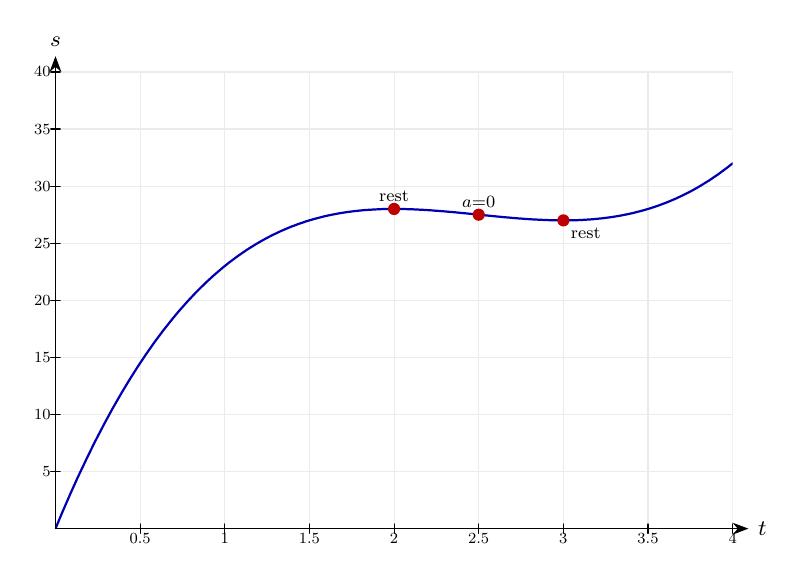
\begin{tikzpicture}[>={Stealth[length=2mm]},font=\footnotesize,line cap=round,line join=round]
\begin{scope}
\clip (0,0) rectangle (8.6,5.8);
\draw[gray!16] (0,0) grid[xstep=1.075,ystep=0.725] (8.6,5.8);
\draw[blue!70!black,thick] (0,0) -- (0.031,0.074) -- (0.061,0.147) -- (0.092,0.22) -- (0.123,0.291) -- (0.154,0.362) -- (0.184,0.432) -- (0.215,0.501) -- (0.246,0.569) -- (0.276,0.636) -- (0.307,0.702) -- (0.338,0.768) -- (0.369,0.832) -- (0.399,0.896) -- (0.43,0.959) -- (0.461,1.022) -- (0.491,1.083) -- (0.522,1.144) -- (0.553,1.203) -- (0.584,1.262) -- (0.614,1.321) -- (0.645,1.378) -- (0.676,1.435) -- (0.706,1.491) -- (0.737,1.546) -- (0.768,1.6) -- (0.799,1.654) -- (0.829,1.706) -- (0.86,1.759) -- (0.891,1.81) -- (0.921,1.86) -- (0.952,1.91) -- (0.983,1.959) -- (1.014,2.008) -- (1.044,2.056) -- (1.075,2.103) -- (1.106,2.149) -- (1.136,2.194) -- (1.167,2.239) -- (1.198,2.283) -- (1.229,2.327) -- (1.259,2.37) -- (1.29,2.412) -- (1.321,2.453) -- (1.351,2.494) -- (1.382,2.534) -- (1.413,2.573) -- (1.444,2.612) -- (1.474,2.65) -- (1.505,2.688) -- (1.536,2.725) -- (1.566,2.761) -- (1.597,2.796) -- (1.628,2.831) -- (1.659,2.866) -- (1.689,2.899) -- (1.72,2.932) -- (1.751,2.965) -- (1.781,2.997) -- (1.812,3.028) -- (1.843,3.059) -- (1.874,3.089) -- (1.904,3.119) -- (1.935,3.148) -- (1.966,3.176) -- (1.996,3.204) -- (2.027,3.231) -- (2.058,3.258) -- (2.089,3.284) -- (2.119,3.31) -- (2.15,3.335) -- (2.181,3.36) -- (2.211,3.384) -- (2.242,3.407) -- (2.273,3.43) -- (2.304,3.453) -- (2.334,3.475) -- (2.365,3.496) -- (2.396,3.517) -- (2.426,3.538) -- (2.457,3.558) -- (2.488,3.577) -- (2.519,3.596) -- (2.549,3.615) -- (2.58,3.633) -- (2.611,3.651) -- (2.641,3.668) -- (2.672,3.685) -- (2.703,3.701) -- (2.734,3.717) -- (2.764,3.732) -- (2.795,3.747) -- (2.826,3.762) -- (2.856,3.776) -- (2.887,3.79) -- (2.918,3.803) -- (2.949,3.816) -- (2.979,3.829) -- (3.01,3.841) -- (3.041,3.852) -- (3.071,3.864) -- (3.102,3.875) -- (3.133,3.885) -- (3.164,3.896) -- (3.194,3.906) -- (3.225,3.915) -- (3.256,3.924) -- (3.286,3.933) -- (3.317,3.941) -- (3.348,3.949) -- (3.379,3.957) -- (3.409,3.965) -- (3.44,3.972) -- (3.471,3.979) -- (3.501,3.985) -- (3.532,3.991) -- (3.563,3.997) -- (3.594,4.003) -- (3.624,4.008) -- (3.655,4.013) -- (3.686,4.018) -- (3.716,4.022) -- (3.747,4.026) -- (3.778,4.03) -- (3.809,4.034) -- (3.839,4.037) -- (3.87,4.04) -- (3.901,4.043) -- (3.931,4.046) -- (3.962,4.048) -- (3.993,4.05) -- (4.024,4.052) -- (4.054,4.054) -- (4.085,4.055) -- (4.116,4.057) -- (4.146,4.058) -- (4.177,4.059) -- (4.208,4.059) -- (4.239,4.06) -- (4.269,4.06) -- (4.3,4.06) -- (4.331,4.06) -- (4.361,4.06) -- (4.392,4.059) -- (4.423,4.059) -- (4.454,4.058) -- (4.484,4.057) -- (4.515,4.056) -- (4.546,4.055) -- (4.576,4.053) -- (4.607,4.052) -- (4.638,4.05) -- (4.669,4.049) -- (4.699,4.047) -- (4.73,4.045) -- (4.761,4.043) -- (4.791,4.041) -- (4.822,4.038) -- (4.853,4.036) -- (4.884,4.034) -- (4.914,4.031) -- (4.945,4.029) -- (4.976,4.026) -- (5.006,4.023) -- (5.037,4.021) -- (5.068,4.018) -- (5.099,4.015) -- (5.129,4.012) -- (5.16,4.009) -- (5.191,4.006) -- (5.221,4.003) -- (5.252,4) -- (5.283,3.997) -- (5.314,3.994) -- (5.344,3.991) -- (5.375,3.987) -- (5.406,3.984) -- (5.436,3.981) -- (5.467,3.978) -- (5.498,3.975) -- (5.529,3.972) -- (5.559,3.969) -- (5.59,3.966) -- (5.621,3.963) -- (5.651,3.96) -- (5.682,3.957) -- (5.713,3.954) -- (5.744,3.952) -- (5.774,3.949) -- (5.805,3.946) -- (5.836,3.944) -- (5.866,3.941) -- (5.897,3.939) -- (5.928,3.937) -- (5.959,3.934) -- (5.989,3.932) -- (6.02,3.93) -- (6.051,3.928) -- (6.081,3.926) -- (6.112,3.925) -- (6.143,3.923) -- (6.174,3.922) -- (6.204,3.92) -- (6.235,3.919) -- (6.266,3.918) -- (6.296,3.917) -- (6.327,3.916) -- (6.358,3.916) -- (6.389,3.915) -- (6.419,3.915) -- (6.45,3.915) -- (6.481,3.915) -- (6.511,3.915) -- (6.542,3.916) -- (6.573,3.916) -- (6.604,3.917) -- (6.634,3.918) -- (6.665,3.92) -- (6.696,3.921) -- (6.726,3.923) -- (6.757,3.925) -- (6.788,3.927) -- (6.819,3.929) -- (6.849,3.932) -- (6.88,3.935) -- (6.911,3.938) -- (6.941,3.941) -- (6.972,3.945) -- (7.003,3.949) -- (7.034,3.953) -- (7.064,3.957) -- (7.095,3.962) -- (7.126,3.967) -- (7.156,3.972) -- (7.187,3.978) -- (7.218,3.984) -- (7.249,3.99) -- (7.279,3.996) -- (7.31,4.003) -- (7.341,4.01) -- (7.371,4.018) -- (7.402,4.026) -- (7.433,4.034) -- (7.464,4.042) -- (7.494,4.051) -- (7.525,4.06) -- (7.556,4.069) -- (7.586,4.079) -- (7.617,4.09) -- (7.648,4.1) -- (7.679,4.111) -- (7.709,4.123) -- (7.74,4.134) -- (7.771,4.146) -- (7.801,4.159) -- (7.832,4.172) -- (7.863,4.185) -- (7.894,4.199) -- (7.924,4.213) -- (7.955,4.228) -- (7.986,4.243) -- (8.016,4.258) -- (8.047,4.274) -- (8.078,4.29) -- (8.109,4.307) -- (8.139,4.324) -- (8.17,4.342) -- (8.201,4.36) -- (8.231,4.379) -- (8.262,4.398) -- (8.293,4.417) -- (8.324,4.437) -- (8.354,4.458) -- (8.385,4.479) -- (8.416,4.5) -- (8.446,4.522) -- (8.477,4.545) -- (8.508,4.568) -- (8.539,4.591) -- (8.569,4.615) -- (8.6,4.64);
\end{scope}
\draw[->] (0,0) -- (8.8,0) node[right]{$t$};
\draw[->] (0,0) -- (0,6) node[above]{$s$};
\draw (1.075,-0.06) -- (1.075,0.06) node[below=1pt,scale=0.7]{$0.5$};
\draw (2.15,-0.06) -- (2.15,0.06) node[below=1pt,scale=0.7]{$1$};
\draw (3.225,-0.06) -- (3.225,0.06) node[below=1pt,scale=0.7]{$1.5$};
\draw (4.3,-0.06) -- (4.3,0.06) node[below=1pt,scale=0.7]{$2$};
\draw (5.375,-0.06) -- (5.375,0.06) node[below=1pt,scale=0.7]{$2.5$};
\draw (6.45,-0.06) -- (6.45,0.06) node[below=1pt,scale=0.7]{$3$};
\draw (7.525,-0.06) -- (7.525,0.06) node[below=1pt,scale=0.7]{$3.5$};
\draw (8.6,-0.06) -- (8.6,0.06) node[below=1pt,scale=0.7]{$4$};
\draw (-0.06,0.725) -- (0.06,0.725) node[left=1pt,scale=0.7]{$5$};
\draw (-0.06,1.45) -- (0.06,1.45) node[left=1pt,scale=0.7]{$10$};
\draw (-0.06,2.175) -- (0.06,2.175) node[left=1pt,scale=0.7]{$15$};
\draw (-0.06,2.9) -- (0.06,2.9) node[left=1pt,scale=0.7]{$20$};
\draw (-0.06,3.625) -- (0.06,3.625) node[left=1pt,scale=0.7]{$25$};
\draw (-0.06,4.35) -- (0.06,4.35) node[left=1pt,scale=0.7]{$30$};
\draw (-0.06,5.075) -- (0.06,5.075) node[left=1pt,scale=0.7]{$35$};
\draw (-0.06,5.8) -- (0.06,5.8) node[left=1pt,scale=0.7]{$40$};
\fill[red!75!black] (4.3,4.06) circle (2.2pt);
\node[above,scale=0.78] at (4.3,4.06) {rest};
\fill[red!75!black] (6.45,3.915) circle (2.2pt);
\node[below right,scale=0.78] at (6.45,3.915) {rest};
\fill[red!75!black] (5.375,3.987) circle (2.2pt);
\node[above,scale=0.78] at (5.375,3.987) {$a{=}0$};
\end{tikzpicture}
}
\end{center}
\small The model plotted against its variable, with the key point(s) marked.\normalsize

\medskip\hrule

\section*{Real-Life Problems 07\quad\small\texttt{(d5-007)}}
\addcontentsline{toc}{section}{Real-Life Problems 07 (d5-007)}
\textit{Difficulty: Foundation \quad\textbar\quad Marks: 4}

\question{A particle moves so that its displacement is \( s = 5t - t^2 \) metres for \( 0 \leq t \leq 5 \). (a) Find the velocity function. (b) Find the time when the particle changes direction. (c) Find the maximum displacement from the starting point.}

\textbf{Worked solution.}

\textit{Step 1: (a) Differentiate.}
\[\begin{gathered}
v = \frac{\mathrm{d}s}{\mathrm{d}t} = 5 - 2t
\end{gathered}\]
Power rule.

\textit{Step 2: (b) The particle changes direction when \( v = 0 \).}
\[\begin{gathered}
5 - 2t = 0 \implies t = 2.5 \text{ s}
\end{gathered}\]
Velocity changes sign here: positive before, negative after $\to$ particle reverses.

\textit{Step 3: (c) Maximum displacement at \( t = 2.5 \).}
\[\begin{gathered}
s = 5(2.5) - (2.5)^2 = 12.5 - 6.25 = 6.25 \text{ m}
\end{gathered}\]
Substitute \( t = 2.5 \) into \( s \).

\begin{answerbox}
\textbf{Final answer:}\quad (a) \(\displaystyle  v = 5 - 2t \) \\[3pt]  (b) \(\displaystyle  t = 2.5 \) s \\[3pt]  (c) Maximum displacement \(\displaystyle  = 6.25 \) m
\end{answerbox}
\textbf{Diagram.}

\begin{center}
\resizebox{\ifdim\width>\linewidth \linewidth\else \width\fi}{!}{%
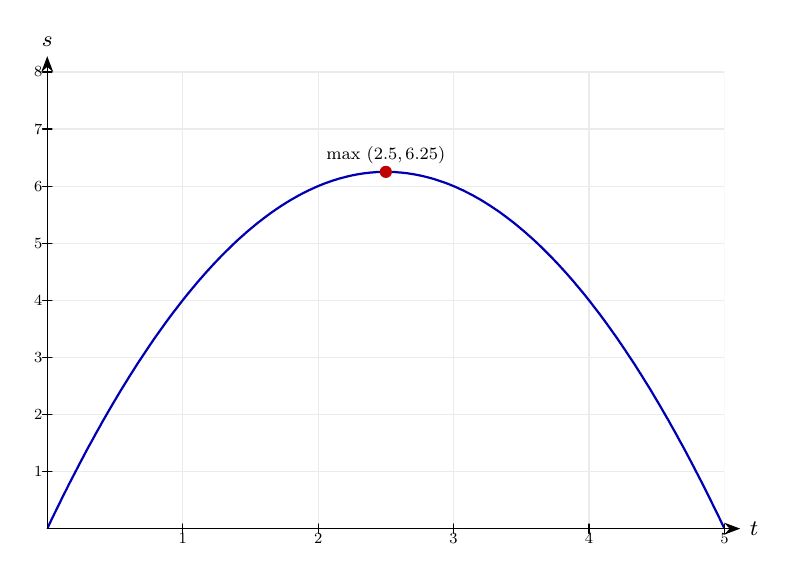
\begin{tikzpicture}[>={Stealth[length=2mm]},font=\footnotesize,line cap=round,line join=round]
\begin{scope}
\clip (0,0) rectangle (8.6,5.8);
\draw[gray!16] (0,0) grid[xstep=1.72,ystep=0.725] (8.6,5.8);
\draw[blue!70!black,thick] (0,0) -- (0.031,0.065) -- (0.061,0.129) -- (0.092,0.192) -- (0.123,0.255) -- (0.154,0.318) -- (0.184,0.38) -- (0.215,0.442) -- (0.246,0.503) -- (0.276,0.564) -- (0.307,0.624) -- (0.338,0.684) -- (0.369,0.743) -- (0.399,0.802) -- (0.43,0.861) -- (0.461,0.919) -- (0.491,0.977) -- (0.522,1.034) -- (0.553,1.09) -- (0.584,1.146) -- (0.614,1.202) -- (0.645,1.257) -- (0.676,1.312) -- (0.706,1.367) -- (0.737,1.42) -- (0.768,1.474) -- (0.799,1.527) -- (0.829,1.579) -- (0.86,1.631) -- (0.891,1.683) -- (0.921,1.734) -- (0.952,1.785) -- (0.983,1.835) -- (1.014,1.884) -- (1.044,1.934) -- (1.075,1.982) -- (1.106,2.031) -- (1.136,2.079) -- (1.167,2.126) -- (1.198,2.173) -- (1.229,2.219) -- (1.259,2.265) -- (1.29,2.311) -- (1.321,2.356) -- (1.351,2.401) -- (1.382,2.445) -- (1.413,2.488) -- (1.444,2.532) -- (1.474,2.574) -- (1.505,2.617) -- (1.536,2.659) -- (1.566,2.7) -- (1.597,2.741) -- (1.628,2.781) -- (1.659,2.821) -- (1.689,2.861) -- (1.72,2.9) -- (1.751,2.939) -- (1.781,2.977) -- (1.812,3.014) -- (1.843,3.052) -- (1.874,3.088) -- (1.904,3.125) -- (1.935,3.161) -- (1.966,3.196) -- (1.996,3.231) -- (2.027,3.265) -- (2.058,3.299) -- (2.089,3.333) -- (2.119,3.366) -- (2.15,3.398) -- (2.181,3.431) -- (2.211,3.462) -- (2.242,3.493) -- (2.273,3.524) -- (2.304,3.554) -- (2.334,3.584) -- (2.365,3.614) -- (2.396,3.643) -- (2.426,3.671) -- (2.457,3.699) -- (2.488,3.726) -- (2.519,3.754) -- (2.549,3.78) -- (2.58,3.806) -- (2.611,3.832) -- (2.641,3.857) -- (2.672,3.882) -- (2.703,3.906) -- (2.734,3.93) -- (2.764,3.953) -- (2.795,3.976) -- (2.826,3.999) -- (2.856,4.021) -- (2.887,4.042) -- (2.918,4.063) -- (2.949,4.084) -- (2.979,4.104) -- (3.01,4.123) -- (3.041,4.143) -- (3.071,4.161) -- (3.102,4.18) -- (3.133,4.197) -- (3.164,4.215) -- (3.194,4.232) -- (3.225,4.248) -- (3.256,4.264) -- (3.286,4.279) -- (3.317,4.295) -- (3.348,4.309) -- (3.379,4.323) -- (3.409,4.337) -- (3.44,4.35) -- (3.471,4.363) -- (3.501,4.375) -- (3.532,4.387) -- (3.563,4.398) -- (3.594,4.409) -- (3.624,4.419) -- (3.655,4.429) -- (3.686,4.439) -- (3.716,4.448) -- (3.747,4.456) -- (3.778,4.464) -- (3.809,4.472) -- (3.839,4.479) -- (3.87,4.486) -- (3.901,4.492) -- (3.931,4.498) -- (3.962,4.503) -- (3.993,4.508) -- (4.024,4.513) -- (4.054,4.516) -- (4.085,4.52) -- (4.116,4.523) -- (4.146,4.525) -- (4.177,4.528) -- (4.208,4.529) -- (4.239,4.53) -- (4.269,4.531) -- (4.3,4.531) -- (4.331,4.531) -- (4.361,4.53) -- (4.392,4.529) -- (4.423,4.528) -- (4.454,4.525) -- (4.484,4.523) -- (4.515,4.52) -- (4.546,4.516) -- (4.576,4.513) -- (4.607,4.508) -- (4.638,4.503) -- (4.669,4.498) -- (4.699,4.492) -- (4.73,4.486) -- (4.761,4.479) -- (4.791,4.472) -- (4.822,4.464) -- (4.853,4.456) -- (4.884,4.448) -- (4.914,4.439) -- (4.945,4.429) -- (4.976,4.419) -- (5.006,4.409) -- (5.037,4.398) -- (5.068,4.387) -- (5.099,4.375) -- (5.129,4.363) -- (5.16,4.35) -- (5.191,4.337) -- (5.221,4.323) -- (5.252,4.309) -- (5.283,4.295) -- (5.314,4.279) -- (5.344,4.264) -- (5.375,4.248) -- (5.406,4.232) -- (5.436,4.215) -- (5.467,4.197) -- (5.498,4.18) -- (5.529,4.161) -- (5.559,4.143) -- (5.59,4.123) -- (5.621,4.104) -- (5.651,4.084) -- (5.682,4.063) -- (5.713,4.042) -- (5.744,4.021) -- (5.774,3.999) -- (5.805,3.976) -- (5.836,3.953) -- (5.866,3.93) -- (5.897,3.906) -- (5.928,3.882) -- (5.959,3.857) -- (5.989,3.832) -- (6.02,3.806) -- (6.051,3.78) -- (6.081,3.754) -- (6.112,3.726) -- (6.143,3.699) -- (6.174,3.671) -- (6.204,3.643) -- (6.235,3.614) -- (6.266,3.584) -- (6.296,3.554) -- (6.327,3.524) -- (6.358,3.493) -- (6.389,3.462) -- (6.419,3.431) -- (6.45,3.398) -- (6.481,3.366) -- (6.511,3.333) -- (6.542,3.299) -- (6.573,3.265) -- (6.604,3.231) -- (6.634,3.196) -- (6.665,3.161) -- (6.696,3.125) -- (6.726,3.088) -- (6.757,3.052) -- (6.788,3.014) -- (6.819,2.977) -- (6.849,2.939) -- (6.88,2.9) -- (6.911,2.861) -- (6.941,2.821) -- (6.972,2.781) -- (7.003,2.741) -- (7.034,2.7) -- (7.064,2.659) -- (7.095,2.617) -- (7.126,2.574) -- (7.156,2.532) -- (7.187,2.488) -- (7.218,2.445) -- (7.249,2.401) -- (7.279,2.356) -- (7.31,2.311) -- (7.341,2.265) -- (7.371,2.219) -- (7.402,2.173) -- (7.433,2.126) -- (7.464,2.079) -- (7.494,2.031) -- (7.525,1.982) -- (7.556,1.934) -- (7.586,1.884) -- (7.617,1.835) -- (7.648,1.785) -- (7.679,1.734) -- (7.709,1.683) -- (7.74,1.631) -- (7.771,1.579) -- (7.801,1.527) -- (7.832,1.474) -- (7.863,1.42) -- (7.894,1.367) -- (7.924,1.312) -- (7.955,1.257) -- (7.986,1.202) -- (8.016,1.146) -- (8.047,1.09) -- (8.078,1.034) -- (8.109,0.977) -- (8.139,0.919) -- (8.17,0.861) -- (8.201,0.802) -- (8.231,0.743) -- (8.262,0.684) -- (8.293,0.624) -- (8.324,0.564) -- (8.354,0.503) -- (8.385,0.442) -- (8.416,0.38) -- (8.446,0.318) -- (8.477,0.255) -- (8.508,0.192) -- (8.539,0.129) -- (8.569,0.065) -- (8.6,0);
\end{scope}
\draw[->] (0,0) -- (8.8,0) node[right]{$t$};
\draw[->] (0,0) -- (0,6) node[above]{$s$};
\draw (1.72,-0.06) -- (1.72,0.06) node[below=1pt,scale=0.7]{$1$};
\draw (3.44,-0.06) -- (3.44,0.06) node[below=1pt,scale=0.7]{$2$};
\draw (5.16,-0.06) -- (5.16,0.06) node[below=1pt,scale=0.7]{$3$};
\draw (6.88,-0.06) -- (6.88,0.06) node[below=1pt,scale=0.7]{$4$};
\draw (8.6,-0.06) -- (8.6,0.06) node[below=1pt,scale=0.7]{$5$};
\draw (-0.06,0.725) -- (0.06,0.725) node[left=1pt,scale=0.7]{$1$};
\draw (-0.06,1.45) -- (0.06,1.45) node[left=1pt,scale=0.7]{$2$};
\draw (-0.06,2.175) -- (0.06,2.175) node[left=1pt,scale=0.7]{$3$};
\draw (-0.06,2.9) -- (0.06,2.9) node[left=1pt,scale=0.7]{$4$};
\draw (-0.06,3.625) -- (0.06,3.625) node[left=1pt,scale=0.7]{$5$};
\draw (-0.06,4.35) -- (0.06,4.35) node[left=1pt,scale=0.7]{$6$};
\draw (-0.06,5.075) -- (0.06,5.075) node[left=1pt,scale=0.7]{$7$};
\draw (-0.06,5.8) -- (0.06,5.8) node[left=1pt,scale=0.7]{$8$};
\fill[red!75!black] (4.3,4.531) circle (2.2pt);
\node[above,scale=0.78] at (4.3,4.531) {max $(2.5,6.25)$};
\end{tikzpicture}
}
\end{center}
\small The model plotted against its variable, with the key point(s) marked.\normalsize

\medskip\hrule

\section*{Real-Life Problems 08\quad\small\texttt{(d5-008)}}
\addcontentsline{toc}{section}{Real-Life Problems 08 (d5-008)}
\textit{Difficulty: Foundation \quad\textbar\quad Marks: 3}

\question{A ball is dropped from a height. Its velocity \( v \) ms\(^{-1}\) after \( t \) seconds is \( v = 10t \). (a) Find the acceleration of the ball. (b) Find the time taken for the ball to reach \( 35 \text{ ms}^{-1} \).}

\textbf{Worked solution.}

\textit{Step 1: (a) Differentiate \( v \) with respect to \( t \).}
\[\begin{gathered}
a = \frac{\mathrm{d}v}{\mathrm{d}t} = 10 \text{ ms}^{-2}
\end{gathered}\]
The acceleration is constant --- this approximates free-fall under gravity.

\textit{Step 2: (b) Set \( v = 35 \).}
\[\begin{gathered}
10t = 35 \implies t = 3.5 \text{ s}
\end{gathered}\]
Solve for \( t \).

\begin{answerbox}
\textbf{Final answer:}\quad (a) \(\displaystyle  a = 10 \text{ ms}^{-2} \) \\[3pt]  (b) \(\displaystyle  t = 3.5 \) s
\end{answerbox}
\textbf{Diagram.}

\begin{center}
\resizebox{\ifdim\width>\linewidth \linewidth\else \width\fi}{!}{%
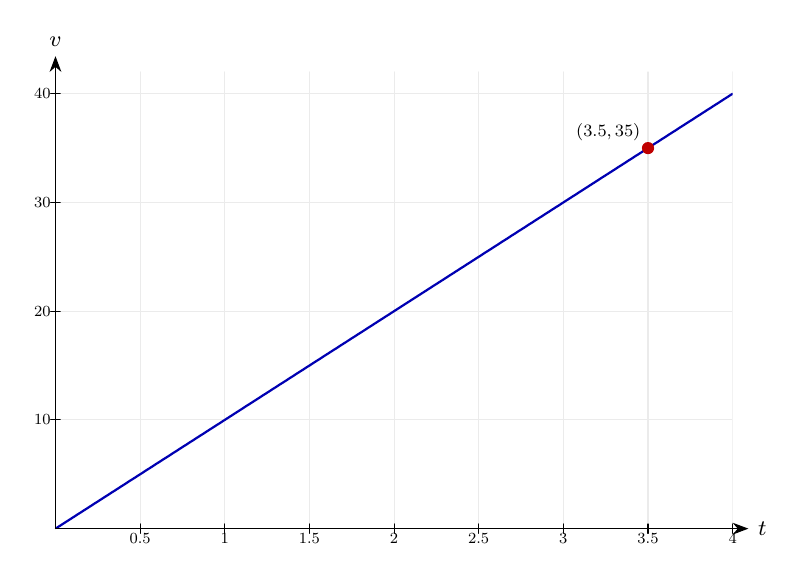
\begin{tikzpicture}[>={Stealth[length=2mm]},font=\footnotesize,line cap=round,line join=round]
\begin{scope}
\clip (0,0) rectangle (8.6,5.8);
\draw[gray!16] (0,0) grid[xstep=1.075,ystep=1.381] (8.6,5.8);
\draw[blue!70!black,thick] (0,0) -- (0.031,0.02) -- (0.061,0.039) -- (0.092,0.059) -- (0.123,0.079) -- (0.154,0.099) -- (0.184,0.118) -- (0.215,0.138) -- (0.246,0.158) -- (0.276,0.178) -- (0.307,0.197) -- (0.338,0.217) -- (0.369,0.237) -- (0.399,0.256) -- (0.43,0.276) -- (0.461,0.296) -- (0.491,0.316) -- (0.522,0.335) -- (0.553,0.355) -- (0.584,0.375) -- (0.614,0.395) -- (0.645,0.414) -- (0.676,0.434) -- (0.706,0.454) -- (0.737,0.473) -- (0.768,0.493) -- (0.799,0.513) -- (0.829,0.533) -- (0.86,0.552) -- (0.891,0.572) -- (0.921,0.592) -- (0.952,0.612) -- (0.983,0.631) -- (1.014,0.651) -- (1.044,0.671) -- (1.075,0.69) -- (1.106,0.71) -- (1.136,0.73) -- (1.167,0.75) -- (1.198,0.769) -- (1.229,0.789) -- (1.259,0.809) -- (1.29,0.829) -- (1.321,0.848) -- (1.351,0.868) -- (1.382,0.888) -- (1.413,0.907) -- (1.444,0.927) -- (1.474,0.947) -- (1.505,0.967) -- (1.536,0.986) -- (1.566,1.006) -- (1.597,1.026) -- (1.628,1.046) -- (1.659,1.065) -- (1.689,1.085) -- (1.72,1.105) -- (1.751,1.124) -- (1.781,1.144) -- (1.812,1.164) -- (1.843,1.184) -- (1.874,1.203) -- (1.904,1.223) -- (1.935,1.243) -- (1.966,1.263) -- (1.996,1.282) -- (2.027,1.302) -- (2.058,1.322) -- (2.089,1.341) -- (2.119,1.361) -- (2.15,1.381) -- (2.181,1.401) -- (2.211,1.42) -- (2.242,1.44) -- (2.273,1.46) -- (2.304,1.48) -- (2.334,1.499) -- (2.365,1.519) -- (2.396,1.539) -- (2.426,1.559) -- (2.457,1.578) -- (2.488,1.598) -- (2.519,1.618) -- (2.549,1.637) -- (2.58,1.657) -- (2.611,1.677) -- (2.641,1.697) -- (2.672,1.716) -- (2.703,1.736) -- (2.734,1.756) -- (2.764,1.776) -- (2.795,1.795) -- (2.826,1.815) -- (2.856,1.835) -- (2.887,1.854) -- (2.918,1.874) -- (2.949,1.894) -- (2.979,1.914) -- (3.01,1.933) -- (3.041,1.953) -- (3.071,1.973) -- (3.102,1.993) -- (3.133,2.012) -- (3.164,2.032) -- (3.194,2.052) -- (3.225,2.071) -- (3.256,2.091) -- (3.286,2.111) -- (3.317,2.131) -- (3.348,2.15) -- (3.379,2.17) -- (3.409,2.19) -- (3.44,2.21) -- (3.471,2.229) -- (3.501,2.249) -- (3.532,2.269) -- (3.563,2.288) -- (3.594,2.308) -- (3.624,2.328) -- (3.655,2.348) -- (3.686,2.367) -- (3.716,2.387) -- (3.747,2.407) -- (3.778,2.427) -- (3.809,2.446) -- (3.839,2.466) -- (3.87,2.486) -- (3.901,2.505) -- (3.931,2.525) -- (3.962,2.545) -- (3.993,2.565) -- (4.024,2.584) -- (4.054,2.604) -- (4.085,2.624) -- (4.116,2.644) -- (4.146,2.663) -- (4.177,2.683) -- (4.208,2.703) -- (4.239,2.722) -- (4.269,2.742) -- (4.3,2.762) -- (4.331,2.782) -- (4.361,2.801) -- (4.392,2.821) -- (4.423,2.841) -- (4.454,2.861) -- (4.484,2.88) -- (4.515,2.9) -- (4.546,2.92) -- (4.576,2.939) -- (4.607,2.959) -- (4.638,2.979) -- (4.669,2.999) -- (4.699,3.018) -- (4.73,3.038) -- (4.761,3.058) -- (4.791,3.078) -- (4.822,3.097) -- (4.853,3.117) -- (4.884,3.137) -- (4.914,3.156) -- (4.945,3.176) -- (4.976,3.196) -- (5.006,3.216) -- (5.037,3.235) -- (5.068,3.255) -- (5.099,3.275) -- (5.129,3.295) -- (5.16,3.314) -- (5.191,3.334) -- (5.221,3.354) -- (5.252,3.373) -- (5.283,3.393) -- (5.314,3.413) -- (5.344,3.433) -- (5.375,3.452) -- (5.406,3.472) -- (5.436,3.492) -- (5.467,3.512) -- (5.498,3.531) -- (5.529,3.551) -- (5.559,3.571) -- (5.59,3.59) -- (5.621,3.61) -- (5.651,3.63) -- (5.682,3.65) -- (5.713,3.669) -- (5.744,3.689) -- (5.774,3.709) -- (5.805,3.729) -- (5.836,3.748) -- (5.866,3.768) -- (5.897,3.788) -- (5.928,3.807) -- (5.959,3.827) -- (5.989,3.847) -- (6.02,3.867) -- (6.051,3.886) -- (6.081,3.906) -- (6.112,3.926) -- (6.143,3.946) -- (6.174,3.965) -- (6.204,3.985) -- (6.235,4.005) -- (6.266,4.024) -- (6.296,4.044) -- (6.327,4.064) -- (6.358,4.084) -- (6.389,4.103) -- (6.419,4.123) -- (6.45,4.143) -- (6.481,4.163) -- (6.511,4.182) -- (6.542,4.202) -- (6.573,4.222) -- (6.604,4.241) -- (6.634,4.261) -- (6.665,4.281) -- (6.696,4.301) -- (6.726,4.32) -- (6.757,4.34) -- (6.788,4.36) -- (6.819,4.38) -- (6.849,4.399) -- (6.88,4.419) -- (6.911,4.439) -- (6.941,4.459) -- (6.972,4.478) -- (7.003,4.498) -- (7.034,4.518) -- (7.064,4.537) -- (7.095,4.557) -- (7.126,4.577) -- (7.156,4.597) -- (7.187,4.616) -- (7.218,4.636) -- (7.249,4.656) -- (7.279,4.676) -- (7.31,4.695) -- (7.341,4.715) -- (7.371,4.735) -- (7.402,4.754) -- (7.433,4.774) -- (7.464,4.794) -- (7.494,4.814) -- (7.525,4.833) -- (7.556,4.853) -- (7.586,4.873) -- (7.617,4.893) -- (7.648,4.912) -- (7.679,4.932) -- (7.709,4.952) -- (7.74,4.971) -- (7.771,4.991) -- (7.801,5.011) -- (7.832,5.031) -- (7.863,5.05) -- (7.894,5.07) -- (7.924,5.09) -- (7.955,5.11) -- (7.986,5.129) -- (8.016,5.149) -- (8.047,5.169) -- (8.078,5.188) -- (8.109,5.208) -- (8.139,5.228) -- (8.17,5.248) -- (8.201,5.267) -- (8.231,5.287) -- (8.262,5.307) -- (8.293,5.327) -- (8.324,5.346) -- (8.354,5.366) -- (8.385,5.386) -- (8.416,5.405) -- (8.446,5.425) -- (8.477,5.445) -- (8.508,5.465) -- (8.539,5.484) -- (8.569,5.504) -- (8.6,5.524);
\end{scope}
\draw[->] (0,0) -- (8.8,0) node[right]{$t$};
\draw[->] (0,0) -- (0,6) node[above]{$v$};
\draw (1.075,-0.06) -- (1.075,0.06) node[below=1pt,scale=0.7]{$0.5$};
\draw (2.15,-0.06) -- (2.15,0.06) node[below=1pt,scale=0.7]{$1$};
\draw (3.225,-0.06) -- (3.225,0.06) node[below=1pt,scale=0.7]{$1.5$};
\draw (4.3,-0.06) -- (4.3,0.06) node[below=1pt,scale=0.7]{$2$};
\draw (5.375,-0.06) -- (5.375,0.06) node[below=1pt,scale=0.7]{$2.5$};
\draw (6.45,-0.06) -- (6.45,0.06) node[below=1pt,scale=0.7]{$3$};
\draw (7.525,-0.06) -- (7.525,0.06) node[below=1pt,scale=0.7]{$3.5$};
\draw (8.6,-0.06) -- (8.6,0.06) node[below=1pt,scale=0.7]{$4$};
\draw (-0.06,1.381) -- (0.06,1.381) node[left=1pt,scale=0.7]{$10$};
\draw (-0.06,2.762) -- (0.06,2.762) node[left=1pt,scale=0.7]{$20$};
\draw (-0.06,4.143) -- (0.06,4.143) node[left=1pt,scale=0.7]{$30$};
\draw (-0.06,5.524) -- (0.06,5.524) node[left=1pt,scale=0.7]{$40$};
\fill[red!75!black] (7.525,4.833) circle (2.2pt);
\node[above left,scale=0.78] at (7.525,4.833) {$(3.5,35)$};
\end{tikzpicture}
}
\end{center}
\small The model plotted against its variable, with the key point(s) marked.\normalsize

\medskip\hrule

\section*{Real-Life Problems 09\quad\small\texttt{(d5-009)}}
\addcontentsline{toc}{section}{Real-Life Problems 09 (d5-009)}
\textit{Difficulty: Foundation \quad\textbar\quad Marks: 5}

\question{A particle's displacement is \( s = t^3 - 4t^2 + 4t \) metres after \( t \) seconds. (a) Find the velocity function. (b) Find the times when the particle is at rest. (c) Find the acceleration when \( t = 1 \).}

\textbf{Worked solution.}

\textit{Step 1: (a) Differentiate.}
\[\begin{gathered}
v = 3t^2 - 8t + 4
\end{gathered}\]
Power rule.

\textit{Step 2: (b) Set \( v = 0 \).}
\[\begin{gathered}
3t^2 - 8t + 4 = 0 \implies (3t - 2)(t - 2) = 0 \implies t = \tfrac{2}{3} \text{ or } t = 2
\end{gathered}\]
Factorise the quadratic.

\textit{Step 3: (c) Acceleration function.}
\[\begin{gathered}
a = \frac{\mathrm{d}v}{\mathrm{d}t} = 6t - 8
\end{gathered}\]
Differentiate \( v \).

\textit{Step 4: Evaluate at \( t = 1 \).}
\[\begin{gathered}
a(1) = 6(1) - 8 = -2 \text{ ms}^{-2}
\end{gathered}\]
The negative sign means the particle is decelerating at this instant.

\begin{answerbox}
\textbf{Final answer:}\quad (a) \(\displaystyle  v = 3t^2 - 8t + 4 \) \\[3pt]  (b) \(\displaystyle  t = \tfrac{2}{3} \) s and \(\displaystyle  t = 2 \) s \\[3pt]  (c) \(\displaystyle  -2 \text{ ms}^{-2} \)
\end{answerbox}
\textbf{Diagram.}

\begin{center}
\resizebox{\ifdim\width>\linewidth \linewidth\else \width\fi}{!}{%
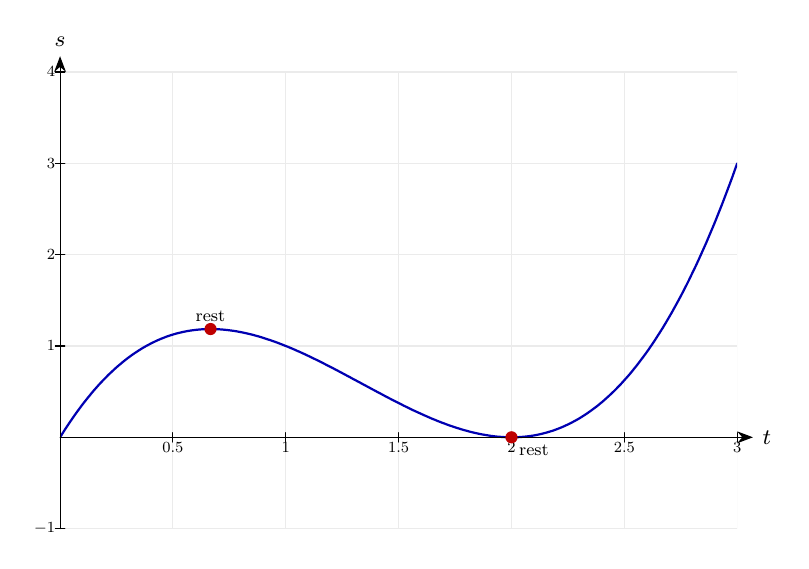
\begin{tikzpicture}[>={Stealth[length=2mm]},font=\footnotesize,line cap=round,line join=round]
\begin{scope}
\clip (0,0) rectangle (8.6,5.8);
\draw[gray!16] (0,0) grid[xstep=1.433,ystep=1.16] (8.6,5.8);
\draw[blue!70!black,thick] (0,1.16) -- (0.031,1.209) -- (0.061,1.257) -- (0.092,1.304) -- (0.123,1.35) -- (0.154,1.395) -- (0.184,1.439) -- (0.215,1.482) -- (0.246,1.524) -- (0.276,1.565) -- (0.307,1.605) -- (0.338,1.644) -- (0.369,1.682) -- (0.399,1.719) -- (0.43,1.756) -- (0.461,1.791) -- (0.491,1.825) -- (0.522,1.858) -- (0.553,1.891) -- (0.584,1.922) -- (0.614,1.953) -- (0.645,1.982) -- (0.676,2.011) -- (0.706,2.039) -- (0.737,2.066) -- (0.768,2.092) -- (0.799,2.118) -- (0.829,2.142) -- (0.86,2.166) -- (0.891,2.189) -- (0.921,2.211) -- (0.952,2.232) -- (0.983,2.252) -- (1.014,2.272) -- (1.044,2.291) -- (1.075,2.309) -- (1.106,2.326) -- (1.136,2.342) -- (1.167,2.358) -- (1.198,2.373) -- (1.229,2.388) -- (1.259,2.401) -- (1.29,2.414) -- (1.321,2.426) -- (1.351,2.438) -- (1.382,2.449) -- (1.413,2.459) -- (1.444,2.468) -- (1.474,2.477) -- (1.505,2.485) -- (1.536,2.492) -- (1.566,2.499) -- (1.597,2.505) -- (1.628,2.511) -- (1.659,2.516) -- (1.689,2.52) -- (1.72,2.524) -- (1.751,2.527) -- (1.781,2.53) -- (1.812,2.532) -- (1.843,2.533) -- (1.874,2.534) -- (1.904,2.535) -- (1.935,2.535) -- (1.966,2.534) -- (1.996,2.533) -- (2.027,2.531) -- (2.058,2.529) -- (2.089,2.526) -- (2.119,2.523) -- (2.15,2.519) -- (2.181,2.515) -- (2.211,2.511) -- (2.242,2.506) -- (2.273,2.5) -- (2.304,2.494) -- (2.334,2.488) -- (2.365,2.481) -- (2.396,2.474) -- (2.426,2.467) -- (2.457,2.459) -- (2.488,2.45) -- (2.519,2.442) -- (2.549,2.433) -- (2.58,2.423) -- (2.611,2.413) -- (2.641,2.403) -- (2.672,2.393) -- (2.703,2.382) -- (2.734,2.371) -- (2.764,2.36) -- (2.795,2.348) -- (2.826,2.336) -- (2.856,2.324) -- (2.887,2.312) -- (2.918,2.299) -- (2.949,2.286) -- (2.979,2.273) -- (3.01,2.259) -- (3.041,2.246) -- (3.071,2.232) -- (3.102,2.218) -- (3.133,2.203) -- (3.164,2.189) -- (3.194,2.174) -- (3.225,2.159) -- (3.256,2.144) -- (3.286,2.129) -- (3.317,2.114) -- (3.348,2.098) -- (3.379,2.082) -- (3.409,2.067) -- (3.44,2.051) -- (3.471,2.035) -- (3.501,2.019) -- (3.532,2.003) -- (3.563,1.986) -- (3.594,1.97) -- (3.624,1.954) -- (3.655,1.937) -- (3.686,1.921) -- (3.716,1.904) -- (3.747,1.888) -- (3.778,1.871) -- (3.809,1.855) -- (3.839,1.838) -- (3.87,1.822) -- (3.901,1.805) -- (3.931,1.789) -- (3.962,1.772) -- (3.993,1.756) -- (4.024,1.739) -- (4.054,1.723) -- (4.085,1.707) -- (4.116,1.69) -- (4.146,1.674) -- (4.177,1.658) -- (4.208,1.642) -- (4.239,1.626) -- (4.269,1.611) -- (4.3,1.595) -- (4.331,1.58) -- (4.361,1.564) -- (4.392,1.549) -- (4.423,1.534) -- (4.454,1.519) -- (4.484,1.504) -- (4.515,1.49) -- (4.546,1.476) -- (4.576,1.462) -- (4.607,1.448) -- (4.638,1.434) -- (4.669,1.421) -- (4.699,1.407) -- (4.73,1.394) -- (4.761,1.382) -- (4.791,1.369) -- (4.822,1.357) -- (4.853,1.345) -- (4.884,1.334) -- (4.914,1.322) -- (4.945,1.311) -- (4.976,1.301) -- (5.006,1.29) -- (5.037,1.28) -- (5.068,1.271) -- (5.099,1.261) -- (5.129,1.252) -- (5.16,1.244) -- (5.191,1.235) -- (5.221,1.227) -- (5.252,1.22) -- (5.283,1.213) -- (5.314,1.206) -- (5.344,1.2) -- (5.375,1.194) -- (5.406,1.189) -- (5.436,1.184) -- (5.467,1.179) -- (5.498,1.175) -- (5.529,1.171) -- (5.559,1.168) -- (5.59,1.166) -- (5.621,1.164) -- (5.651,1.162) -- (5.682,1.161) -- (5.713,1.16) -- (5.744,1.16) -- (5.774,1.16) -- (5.805,1.161) -- (5.836,1.163) -- (5.866,1.165) -- (5.897,1.168) -- (5.928,1.171) -- (5.959,1.175) -- (5.989,1.179) -- (6.02,1.184) -- (6.051,1.19) -- (6.081,1.196) -- (6.112,1.203) -- (6.143,1.211) -- (6.174,1.219) -- (6.204,1.228) -- (6.235,1.237) -- (6.266,1.247) -- (6.296,1.258) -- (6.327,1.27) -- (6.358,1.282) -- (6.389,1.295) -- (6.419,1.309) -- (6.45,1.323) -- (6.481,1.338) -- (6.511,1.354) -- (6.542,1.371) -- (6.573,1.388) -- (6.604,1.406) -- (6.634,1.425) -- (6.665,1.445) -- (6.696,1.465) -- (6.726,1.487) -- (6.757,1.509) -- (6.788,1.532) -- (6.819,1.555) -- (6.849,1.58) -- (6.88,1.605) -- (6.911,1.632) -- (6.941,1.659) -- (6.972,1.687) -- (7.003,1.716) -- (7.034,1.746) -- (7.064,1.776) -- (7.095,1.808) -- (7.126,1.84) -- (7.156,1.874) -- (7.187,1.908) -- (7.218,1.943) -- (7.249,1.979) -- (7.279,2.017) -- (7.31,2.055) -- (7.341,2.094) -- (7.371,2.134) -- (7.402,2.175) -- (7.433,2.217) -- (7.464,2.26) -- (7.494,2.304) -- (7.525,2.349) -- (7.556,2.396) -- (7.586,2.443) -- (7.617,2.491) -- (7.648,2.54) -- (7.679,2.591) -- (7.709,2.642) -- (7.74,2.695) -- (7.771,2.748) -- (7.801,2.803) -- (7.832,2.859) -- (7.863,2.916) -- (7.894,2.974) -- (7.924,3.033) -- (7.955,3.093) -- (7.986,3.155) -- (8.016,3.218) -- (8.047,3.281) -- (8.078,3.346) -- (8.109,3.413) -- (8.139,3.48) -- (8.17,3.549) -- (8.201,3.618) -- (8.231,3.689) -- (8.262,3.762) -- (8.293,3.835) -- (8.324,3.91) -- (8.354,3.986) -- (8.385,4.063) -- (8.416,4.142) -- (8.446,4.221) -- (8.477,4.303) -- (8.508,4.385) -- (8.539,4.469) -- (8.569,4.554) -- (8.6,4.64);
\end{scope}
\draw[->] (0,1.16) -- (8.8,1.16) node[right]{$t$};
\draw[->] (0,0) -- (0,6) node[above]{$s$};
\draw (1.433,1.1) -- (1.433,1.22) node[below=1pt,scale=0.7]{$0.5$};
\draw (2.867,1.1) -- (2.867,1.22) node[below=1pt,scale=0.7]{$1$};
\draw (4.3,1.1) -- (4.3,1.22) node[below=1pt,scale=0.7]{$1.5$};
\draw (5.733,1.1) -- (5.733,1.22) node[below=1pt,scale=0.7]{$2$};
\draw (7.167,1.1) -- (7.167,1.22) node[below=1pt,scale=0.7]{$2.5$};
\draw (8.6,1.1) -- (8.6,1.22) node[below=1pt,scale=0.7]{$3$};
\draw (-0.06,0) -- (0.06,0) node[left=1pt,scale=0.7]{$-1$};
\draw (-0.06,2.32) -- (0.06,2.32) node[left=1pt,scale=0.7]{$1$};
\draw (-0.06,3.48) -- (0.06,3.48) node[left=1pt,scale=0.7]{$2$};
\draw (-0.06,4.64) -- (0.06,4.64) node[left=1pt,scale=0.7]{$3$};
\draw (-0.06,5.8) -- (0.06,5.8) node[left=1pt,scale=0.7]{$4$};
\fill[red!75!black] (1.911,2.535) circle (2.2pt);
\node[above,scale=0.78] at (1.911,2.535) {rest};
\fill[red!75!black] (5.733,1.16) circle (2.2pt);
\node[below right,scale=0.78] at (5.733,1.16) {rest};
\end{tikzpicture}
}
\end{center}
\small The model plotted against its variable, with the key point(s) marked.\normalsize

\medskip\hrule

\section*{Real-Life Problems 10\quad\small\texttt{(d5-010)}}
\addcontentsline{toc}{section}{Real-Life Problems 10 (d5-010)}
\textit{Difficulty: Foundation \quad\textbar\quad Marks: 5}

\question{A rectangular garden has length \( x \) m and width \( y \) m. The perimeter of the garden is \( 60 \) m. (a) Write \( y \) in terms of \( x \). (b) Write down an expression for the area \( A \) in terms of \( x \) only. (c) Use calculus to find the value of \( x \) that maximises the area, and find that maximum area.}

\textbf{Worked solution.}

\textit{Step 1: (a) Use the perimeter condition.}
\[\begin{gathered}
2x + 2y = 60 \implies y = 30 - x
\end{gathered}\]
Rearrange the perimeter formula.

\textit{Step 2: (b) Area expression.}
\[\begin{gathered}
A = xy = x(30 - x) = 30x - x^2
\end{gathered}\]
Substitute \( y = 30 - x \) into \( A = xy \).

\textit{Step 3: (c) Differentiate and set to zero.}
\[\begin{gathered}
\frac{\mathrm{d}A}{\mathrm{d}x} = 30 - 2x = 0 \implies x = 15
\end{gathered}\]
Stationary point at \( x = 15 \).

\textit{Step 4: Confirm maximum.}
\[\begin{gathered}
\frac{\mathrm{d}^2A}{\mathrm{d}x^2} = -2 < 0 \Rightarrow \text{maximum}
\end{gathered}\]
Negative second derivative confirms a maximum.

\textit{Step 5: Find maximum area.}
\[\begin{gathered}
A = 15 \times 15 = 225 \text{ m}^2
\end{gathered}\]
Substitute \( x = 15 \) and \( y = 15 \).

\begin{answerbox}
\textbf{Final answer:}\quad (a) \(\displaystyle  y = 30 - x \) \\[3pt]  (b) \(\displaystyle  A = 30x - x^2 \) \\[3pt]  (c) Maximum area \(\displaystyle  = 225 \text{ m}^2 \) when \(\displaystyle  x = 15 \)
\end{answerbox}
\textbf{Diagram.}

\begin{center}
\resizebox{\ifdim\width>\linewidth \linewidth\else \width\fi}{!}{%
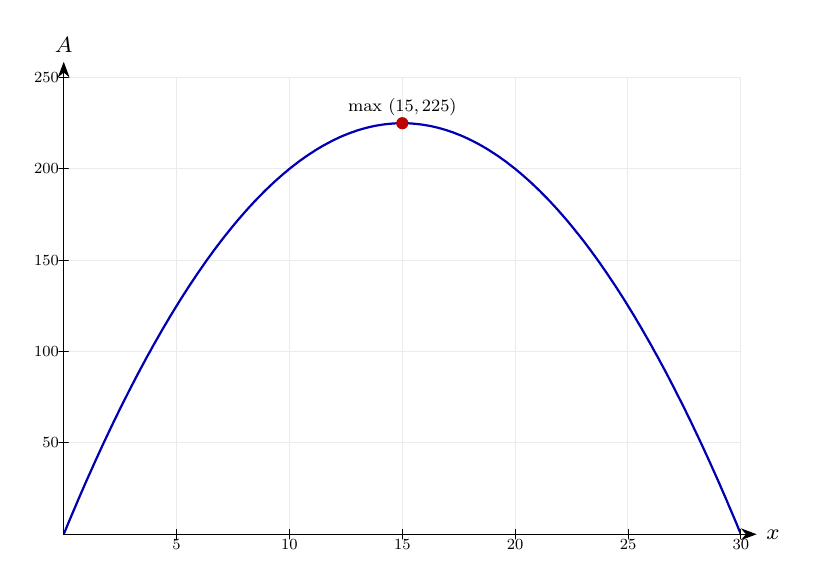
\begin{tikzpicture}[>={Stealth[length=2mm]},font=\footnotesize,line cap=round,line join=round]
\begin{scope}
\clip (0,0) rectangle (8.6,5.8);
\draw[gray!16] (0,0) grid[xstep=1.433,ystep=1.16] (8.6,5.8);
\draw[blue!70!black,thick] (0,0) -- (0.031,0.074) -- (0.061,0.148) -- (0.092,0.221) -- (0.123,0.294) -- (0.154,0.366) -- (0.184,0.438) -- (0.215,0.509) -- (0.246,0.58) -- (0.276,0.65) -- (0.307,0.719) -- (0.338,0.788) -- (0.369,0.857) -- (0.399,0.924) -- (0.43,0.992) -- (0.461,1.059) -- (0.491,1.125) -- (0.522,1.191) -- (0.553,1.256) -- (0.584,1.321) -- (0.614,1.385) -- (0.645,1.449) -- (0.676,1.512) -- (0.706,1.574) -- (0.737,1.636) -- (0.768,1.698) -- (0.799,1.759) -- (0.829,1.819) -- (0.86,1.879) -- (0.891,1.939) -- (0.921,1.997) -- (0.952,2.056) -- (0.983,2.114) -- (1.014,2.171) -- (1.044,2.228) -- (1.075,2.284) -- (1.106,2.339) -- (1.136,2.395) -- (1.167,2.449) -- (1.198,2.503) -- (1.229,2.557) -- (1.259,2.61) -- (1.29,2.662) -- (1.321,2.714) -- (1.351,2.766) -- (1.382,2.816) -- (1.413,2.867) -- (1.444,2.917) -- (1.474,2.966) -- (1.505,3.015) -- (1.536,3.063) -- (1.566,3.11) -- (1.597,3.158) -- (1.628,3.204) -- (1.659,3.25) -- (1.689,3.296) -- (1.72,3.341) -- (1.751,3.385) -- (1.781,3.429) -- (1.812,3.473) -- (1.843,3.516) -- (1.874,3.558) -- (1.904,3.6) -- (1.935,3.641) -- (1.966,3.682) -- (1.996,3.722) -- (2.027,3.762) -- (2.058,3.801) -- (2.089,3.839) -- (2.119,3.877) -- (2.15,3.915) -- (2.181,3.952) -- (2.211,3.989) -- (2.242,4.024) -- (2.273,4.06) -- (2.304,4.095) -- (2.334,4.129) -- (2.365,4.163) -- (2.396,4.196) -- (2.426,4.229) -- (2.457,4.261) -- (2.488,4.293) -- (2.519,4.324) -- (2.549,4.355) -- (2.58,4.385) -- (2.611,4.414) -- (2.641,4.443) -- (2.672,4.472) -- (2.703,4.5) -- (2.734,4.527) -- (2.764,4.554) -- (2.795,4.581) -- (2.826,4.606) -- (2.856,4.632) -- (2.887,4.656) -- (2.918,4.681) -- (2.949,4.704) -- (2.979,4.728) -- (3.01,4.75) -- (3.041,4.772) -- (3.071,4.794) -- (3.102,4.815) -- (3.133,4.835) -- (3.164,4.855) -- (3.194,4.875) -- (3.225,4.894) -- (3.256,4.912) -- (3.286,4.93) -- (3.317,4.947) -- (3.348,4.964) -- (3.379,4.98) -- (3.409,4.996) -- (3.44,5.011) -- (3.471,5.026) -- (3.501,5.04) -- (3.532,5.054) -- (3.563,5.067) -- (3.594,5.079) -- (3.624,5.091) -- (3.655,5.103) -- (3.686,5.113) -- (3.716,5.124) -- (3.747,5.134) -- (3.778,5.143) -- (3.809,5.152) -- (3.839,5.16) -- (3.87,5.168) -- (3.901,5.175) -- (3.931,5.182) -- (3.962,5.188) -- (3.993,5.193) -- (4.024,5.198) -- (4.054,5.203) -- (4.085,5.207) -- (4.116,5.21) -- (4.146,5.213) -- (4.177,5.216) -- (4.208,5.218) -- (4.239,5.219) -- (4.269,5.22) -- (4.3,5.22) -- (4.331,5.22) -- (4.361,5.219) -- (4.392,5.218) -- (4.423,5.216) -- (4.454,5.213) -- (4.484,5.21) -- (4.515,5.207) -- (4.546,5.203) -- (4.576,5.198) -- (4.607,5.193) -- (4.638,5.188) -- (4.669,5.182) -- (4.699,5.175) -- (4.73,5.168) -- (4.761,5.16) -- (4.791,5.152) -- (4.822,5.143) -- (4.853,5.134) -- (4.884,5.124) -- (4.914,5.113) -- (4.945,5.103) -- (4.976,5.091) -- (5.006,5.079) -- (5.037,5.067) -- (5.068,5.054) -- (5.099,5.04) -- (5.129,5.026) -- (5.16,5.011) -- (5.191,4.996) -- (5.221,4.98) -- (5.252,4.964) -- (5.283,4.947) -- (5.314,4.93) -- (5.344,4.912) -- (5.375,4.894) -- (5.406,4.875) -- (5.436,4.855) -- (5.467,4.835) -- (5.498,4.815) -- (5.529,4.794) -- (5.559,4.772) -- (5.59,4.75) -- (5.621,4.728) -- (5.651,4.704) -- (5.682,4.681) -- (5.713,4.656) -- (5.744,4.632) -- (5.774,4.606) -- (5.805,4.581) -- (5.836,4.554) -- (5.866,4.527) -- (5.897,4.5) -- (5.928,4.472) -- (5.959,4.443) -- (5.989,4.414) -- (6.02,4.385) -- (6.051,4.355) -- (6.081,4.324) -- (6.112,4.293) -- (6.143,4.261) -- (6.174,4.229) -- (6.204,4.196) -- (6.235,4.163) -- (6.266,4.129) -- (6.296,4.095) -- (6.327,4.06) -- (6.358,4.024) -- (6.389,3.989) -- (6.419,3.952) -- (6.45,3.915) -- (6.481,3.877) -- (6.511,3.839) -- (6.542,3.801) -- (6.573,3.762) -- (6.604,3.722) -- (6.634,3.682) -- (6.665,3.641) -- (6.696,3.6) -- (6.726,3.558) -- (6.757,3.516) -- (6.788,3.473) -- (6.819,3.429) -- (6.849,3.385) -- (6.88,3.341) -- (6.911,3.296) -- (6.941,3.25) -- (6.972,3.204) -- (7.003,3.158) -- (7.034,3.11) -- (7.064,3.063) -- (7.095,3.015) -- (7.126,2.966) -- (7.156,2.917) -- (7.187,2.867) -- (7.218,2.816) -- (7.249,2.766) -- (7.279,2.714) -- (7.31,2.662) -- (7.341,2.61) -- (7.371,2.557) -- (7.402,2.503) -- (7.433,2.449) -- (7.464,2.395) -- (7.494,2.339) -- (7.525,2.284) -- (7.556,2.228) -- (7.586,2.171) -- (7.617,2.114) -- (7.648,2.056) -- (7.679,1.997) -- (7.709,1.939) -- (7.74,1.879) -- (7.771,1.819) -- (7.801,1.759) -- (7.832,1.698) -- (7.863,1.636) -- (7.894,1.574) -- (7.924,1.512) -- (7.955,1.449) -- (7.986,1.385) -- (8.016,1.321) -- (8.047,1.256) -- (8.078,1.191) -- (8.109,1.125) -- (8.139,1.059) -- (8.17,0.992) -- (8.201,0.924) -- (8.231,0.857) -- (8.262,0.788) -- (8.293,0.719) -- (8.324,0.65) -- (8.354,0.58) -- (8.385,0.509) -- (8.416,0.438) -- (8.446,0.366) -- (8.477,0.294) -- (8.508,0.221) -- (8.539,0.148) -- (8.569,0.074) -- (8.6,0);
\end{scope}
\draw[->] (0,0) -- (8.8,0) node[right]{$x$};
\draw[->] (0,0) -- (0,6) node[above]{$A$};
\draw (1.433,-0.06) -- (1.433,0.06) node[below=1pt,scale=0.7]{$5$};
\draw (2.867,-0.06) -- (2.867,0.06) node[below=1pt,scale=0.7]{$10$};
\draw (4.3,-0.06) -- (4.3,0.06) node[below=1pt,scale=0.7]{$15$};
\draw (5.733,-0.06) -- (5.733,0.06) node[below=1pt,scale=0.7]{$20$};
\draw (7.167,-0.06) -- (7.167,0.06) node[below=1pt,scale=0.7]{$25$};
\draw (8.6,-0.06) -- (8.6,0.06) node[below=1pt,scale=0.7]{$30$};
\draw (-0.06,1.16) -- (0.06,1.16) node[left=1pt,scale=0.7]{$50$};
\draw (-0.06,2.32) -- (0.06,2.32) node[left=1pt,scale=0.7]{$100$};
\draw (-0.06,3.48) -- (0.06,3.48) node[left=1pt,scale=0.7]{$150$};
\draw (-0.06,4.64) -- (0.06,4.64) node[left=1pt,scale=0.7]{$200$};
\draw (-0.06,5.8) -- (0.06,5.8) node[left=1pt,scale=0.7]{$250$};
\fill[red!75!black] (4.3,5.22) circle (2.2pt);
\node[above,scale=0.78] at (4.3,5.22) {max $(15,225)$};
\end{tikzpicture}
}
\end{center}
\small The model plotted against its variable, with the key point(s) marked.\normalsize

\medskip\hrule

\section*{Real-Life Problems 11\quad\small\texttt{(d5-011)}}
\addcontentsline{toc}{section}{Real-Life Problems 11 (d5-011)}
\textit{Difficulty: Foundation \quad\textbar\quad Marks: 5}

\question{A farmer uses \( 80 \) m of fencing to enclose a rectangular field on three sides (the fourth side is a wall). The width of the field is \( x \) m. (a) Show that the area of the field is \( A = x(80 - 2x) \). (b) Find the maximum possible area using calculus.}

\textbf{Worked solution.}

\textit{Step 1: (a) The three sides use \( 2x + l = 80 \), where \( l \) is the length.}
\[\begin{gathered}
l = 80 - 2x \implies A = x \cdot l = x(80 - 2x)
\end{gathered}\]
Two widths \( x \) and one length \( l \) make up the 80 m of fencing.

\textit{Step 2: (b) Expand and differentiate.}
\[\begin{gathered}
A = 80x - 2x^2 \implies \frac{\mathrm{d}A}{\mathrm{d}x} = 80 - 4x
\end{gathered}\]
Power rule.

\textit{Step 3: Set to zero.}
\[\begin{gathered}
80 - 4x = 0 \implies x = 20
\end{gathered}\]
Stationary point at \( x = 20 \).

\textit{Step 4: Confirm maximum and find area.}
\[\begin{gathered}
\frac{\mathrm{d}^2A}{\mathrm{d}x^2} = -4 < 0; \quad A = 20(80 - 40) = 20 \times 40 = 800 \text{ m}^2
\end{gathered}\]
Negative second derivative confirms maximum.

\begin{answerbox}
\textbf{Final answer:}\quad (a) Shown. \\[3pt]  (b) Maximum area \(\displaystyle  = 800 \text{ m}^2 \) when \(\displaystyle  x = 20 \)
\end{answerbox}
\textbf{Diagram.}

\begin{center}
\resizebox{\ifdim\width>\linewidth \linewidth\else \width\fi}{!}{%
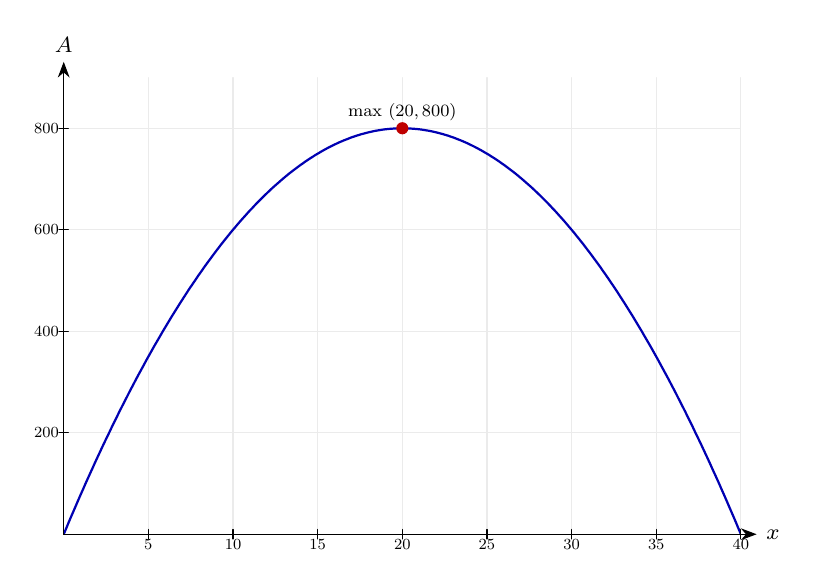
\begin{tikzpicture}[>={Stealth[length=2mm]},font=\footnotesize,line cap=round,line join=round]
\begin{scope}
\clip (0,0) rectangle (8.6,5.8);
\draw[gray!16] (0,0) grid[xstep=1.075,ystep=1.289] (8.6,5.8);
\draw[blue!70!black,thick] (0,0) -- (0.031,0.073) -- (0.061,0.146) -- (0.092,0.219) -- (0.123,0.29) -- (0.154,0.362) -- (0.184,0.432) -- (0.215,0.503) -- (0.246,0.572) -- (0.276,0.642) -- (0.307,0.71) -- (0.338,0.778) -- (0.369,0.846) -- (0.399,0.913) -- (0.43,0.98) -- (0.461,1.046) -- (0.491,1.111) -- (0.522,1.176) -- (0.553,1.24) -- (0.584,1.304) -- (0.614,1.368) -- (0.645,1.431) -- (0.676,1.493) -- (0.706,1.555) -- (0.737,1.616) -- (0.768,1.677) -- (0.799,1.737) -- (0.829,1.797) -- (0.86,1.856) -- (0.891,1.915) -- (0.921,1.973) -- (0.952,2.03) -- (0.983,2.087) -- (1.014,2.144) -- (1.044,2.2) -- (1.075,2.256) -- (1.106,2.311) -- (1.136,2.365) -- (1.167,2.419) -- (1.198,2.472) -- (1.229,2.525) -- (1.259,2.578) -- (1.29,2.629) -- (1.321,2.681) -- (1.351,2.731) -- (1.382,2.782) -- (1.413,2.831) -- (1.444,2.881) -- (1.474,2.929) -- (1.505,2.977) -- (1.536,3.025) -- (1.566,3.072) -- (1.597,3.119) -- (1.628,3.165) -- (1.659,3.21) -- (1.689,3.255) -- (1.72,3.3) -- (1.751,3.343) -- (1.781,3.387) -- (1.812,3.43) -- (1.843,3.472) -- (1.874,3.514) -- (1.904,3.555) -- (1.935,3.596) -- (1.966,3.636) -- (1.996,3.676) -- (2.027,3.715) -- (2.058,3.754) -- (2.089,3.792) -- (2.119,3.83) -- (2.15,3.867) -- (2.181,3.903) -- (2.211,3.939) -- (2.242,3.975) -- (2.273,4.01) -- (2.304,4.044) -- (2.334,4.078) -- (2.365,4.112) -- (2.396,4.144) -- (2.426,4.177) -- (2.457,4.209) -- (2.488,4.24) -- (2.519,4.271) -- (2.549,4.301) -- (2.58,4.331) -- (2.611,4.36) -- (2.641,4.389) -- (2.672,4.417) -- (2.703,4.444) -- (2.734,4.471) -- (2.764,4.498) -- (2.795,4.524) -- (2.826,4.55) -- (2.856,4.575) -- (2.887,4.599) -- (2.918,4.623) -- (2.949,4.646) -- (2.979,4.669) -- (3.01,4.692) -- (3.041,4.713) -- (3.071,4.735) -- (3.102,4.755) -- (3.133,4.776) -- (3.164,4.795) -- (3.194,4.815) -- (3.225,4.833) -- (3.256,4.851) -- (3.286,4.869) -- (3.317,4.886) -- (3.348,4.903) -- (3.379,4.919) -- (3.409,4.934) -- (3.44,4.949) -- (3.471,4.964) -- (3.501,4.978) -- (3.532,4.991) -- (3.563,5.004) -- (3.594,5.016) -- (3.624,5.028) -- (3.655,5.04) -- (3.686,5.05) -- (3.716,5.061) -- (3.747,5.07) -- (3.778,5.08) -- (3.809,5.088) -- (3.839,5.096) -- (3.87,5.104) -- (3.901,5.111) -- (3.931,5.118) -- (3.962,5.124) -- (3.993,5.129) -- (4.024,5.134) -- (4.054,5.139) -- (4.085,5.143) -- (4.116,5.146) -- (4.146,5.149) -- (4.177,5.151) -- (4.208,5.153) -- (4.239,5.155) -- (4.269,5.155) -- (4.3,5.156) -- (4.331,5.155) -- (4.361,5.155) -- (4.392,5.153) -- (4.423,5.151) -- (4.454,5.149) -- (4.484,5.146) -- (4.515,5.143) -- (4.546,5.139) -- (4.576,5.134) -- (4.607,5.129) -- (4.638,5.124) -- (4.669,5.118) -- (4.699,5.111) -- (4.73,5.104) -- (4.761,5.096) -- (4.791,5.088) -- (4.822,5.08) -- (4.853,5.07) -- (4.884,5.061) -- (4.914,5.05) -- (4.945,5.04) -- (4.976,5.028) -- (5.006,5.016) -- (5.037,5.004) -- (5.068,4.991) -- (5.099,4.978) -- (5.129,4.964) -- (5.16,4.949) -- (5.191,4.934) -- (5.221,4.919) -- (5.252,4.903) -- (5.283,4.886) -- (5.314,4.869) -- (5.344,4.851) -- (5.375,4.833) -- (5.406,4.815) -- (5.436,4.795) -- (5.467,4.776) -- (5.498,4.755) -- (5.529,4.735) -- (5.559,4.713) -- (5.59,4.692) -- (5.621,4.669) -- (5.651,4.646) -- (5.682,4.623) -- (5.713,4.599) -- (5.744,4.575) -- (5.774,4.55) -- (5.805,4.524) -- (5.836,4.498) -- (5.866,4.471) -- (5.897,4.444) -- (5.928,4.417) -- (5.959,4.389) -- (5.989,4.36) -- (6.02,4.331) -- (6.051,4.301) -- (6.081,4.271) -- (6.112,4.24) -- (6.143,4.209) -- (6.174,4.177) -- (6.204,4.144) -- (6.235,4.112) -- (6.266,4.078) -- (6.296,4.044) -- (6.327,4.01) -- (6.358,3.975) -- (6.389,3.939) -- (6.419,3.903) -- (6.45,3.867) -- (6.481,3.83) -- (6.511,3.792) -- (6.542,3.754) -- (6.573,3.715) -- (6.604,3.676) -- (6.634,3.636) -- (6.665,3.596) -- (6.696,3.555) -- (6.726,3.514) -- (6.757,3.472) -- (6.788,3.43) -- (6.819,3.387) -- (6.849,3.343) -- (6.88,3.3) -- (6.911,3.255) -- (6.941,3.21) -- (6.972,3.165) -- (7.003,3.119) -- (7.034,3.072) -- (7.064,3.025) -- (7.095,2.977) -- (7.126,2.929) -- (7.156,2.881) -- (7.187,2.831) -- (7.218,2.782) -- (7.249,2.731) -- (7.279,2.681) -- (7.31,2.629) -- (7.341,2.578) -- (7.371,2.525) -- (7.402,2.472) -- (7.433,2.419) -- (7.464,2.365) -- (7.494,2.311) -- (7.525,2.256) -- (7.556,2.2) -- (7.586,2.144) -- (7.617,2.087) -- (7.648,2.03) -- (7.679,1.973) -- (7.709,1.915) -- (7.74,1.856) -- (7.771,1.797) -- (7.801,1.737) -- (7.832,1.677) -- (7.863,1.616) -- (7.894,1.555) -- (7.924,1.493) -- (7.955,1.431) -- (7.986,1.368) -- (8.016,1.304) -- (8.047,1.24) -- (8.078,1.176) -- (8.109,1.111) -- (8.139,1.046) -- (8.17,0.98) -- (8.201,0.913) -- (8.231,0.846) -- (8.262,0.778) -- (8.293,0.71) -- (8.324,0.642) -- (8.354,0.572) -- (8.385,0.503) -- (8.416,0.432) -- (8.446,0.362) -- (8.477,0.29) -- (8.508,0.219) -- (8.539,0.146) -- (8.569,0.073) -- (8.6,0);
\end{scope}
\draw[->] (0,0) -- (8.8,0) node[right]{$x$};
\draw[->] (0,0) -- (0,6) node[above]{$A$};
\draw (1.075,-0.06) -- (1.075,0.06) node[below=1pt,scale=0.7]{$5$};
\draw (2.15,-0.06) -- (2.15,0.06) node[below=1pt,scale=0.7]{$10$};
\draw (3.225,-0.06) -- (3.225,0.06) node[below=1pt,scale=0.7]{$15$};
\draw (4.3,-0.06) -- (4.3,0.06) node[below=1pt,scale=0.7]{$20$};
\draw (5.375,-0.06) -- (5.375,0.06) node[below=1pt,scale=0.7]{$25$};
\draw (6.45,-0.06) -- (6.45,0.06) node[below=1pt,scale=0.7]{$30$};
\draw (7.525,-0.06) -- (7.525,0.06) node[below=1pt,scale=0.7]{$35$};
\draw (8.6,-0.06) -- (8.6,0.06) node[below=1pt,scale=0.7]{$40$};
\draw (-0.06,1.289) -- (0.06,1.289) node[left=1pt,scale=0.7]{$200$};
\draw (-0.06,2.578) -- (0.06,2.578) node[left=1pt,scale=0.7]{$400$};
\draw (-0.06,3.867) -- (0.06,3.867) node[left=1pt,scale=0.7]{$600$};
\draw (-0.06,5.156) -- (0.06,5.156) node[left=1pt,scale=0.7]{$800$};
\fill[red!75!black] (4.3,5.156) circle (2.2pt);
\node[above,scale=0.78] at (4.3,5.156) {max $(20,800)$};
\end{tikzpicture}
}
\end{center}
\small The model plotted against its variable, with the key point(s) marked.\normalsize

\medskip\hrule

\section*{Real-Life Problems 12\quad\small\texttt{(d5-012)}}
\addcontentsline{toc}{section}{Real-Life Problems 12 (d5-012)}
\textit{Difficulty: Foundation \quad\textbar\quad Marks: 5}

\question{A ball is thrown vertically upwards with an initial speed of \( 25 \) ms\(^{-1}\). After \( t \) seconds its height is \( h = 25t - 5t^2 \) metres. (a) Find the height after 1 second. (b) Use calculus to find the maximum height. (c) Find the time when the ball returns to ground level.}

\textbf{Worked solution.}

\textit{Step 1: (a) Substitute \( t = 1 \).}
\[\begin{gathered}
h(1) = 25 - 5 = 20 \text{ m}
\end{gathered}\]
Direct substitution.

\textit{Step 2: (b) Differentiate and set to zero.}
\[\begin{gathered}
\frac{\mathrm{d}h}{\mathrm{d}t} = 25 - 10t = 0 \implies t = 2.5 \text{ s}
\end{gathered}\]
Maximum height when velocity is zero.

\textit{Step 3: Find the maximum height.}
\[\begin{gathered}
h(2.5) = 25(2.5) - 5(6.25) = 62.5 - 31.25 = 31.25 \text{ m}
\end{gathered}\]
Substitute \( t = 2.5 \).

\textit{Step 4: (c) Set \( h = 0 \).}
\[\begin{gathered}
25t - 5t^2 = 0 \implies 5t(5 - t) = 0 \implies t = 0 \text{ or } t = 5
\end{gathered}\]
\( t = 0 \) is the launch; \( t = 5 \) is when it lands.

\begin{answerbox}
\textbf{Final answer:}\quad (a) \(\displaystyle  20 \) m \\[3pt]  (b) \(\displaystyle  31.25 \) m at \(\displaystyle  t = 2.5 \) s \\[3pt]  (c) \(\displaystyle  t = 5 \) s
\end{answerbox}
\textbf{Diagram.}

\begin{center}
\resizebox{\ifdim\width>\linewidth \linewidth\else \width\fi}{!}{%
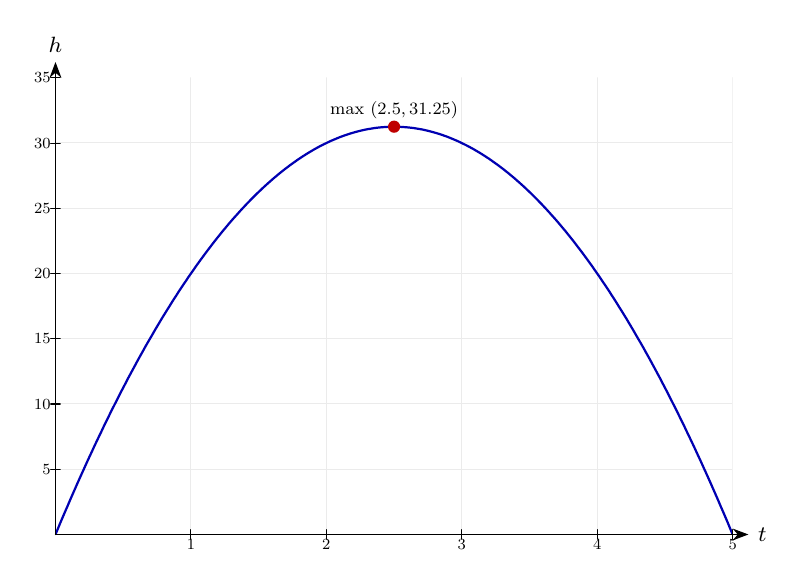
\begin{tikzpicture}[>={Stealth[length=2mm]},font=\footnotesize,line cap=round,line join=round]
\begin{scope}
\clip (0,0) rectangle (8.6,5.8);
\draw[gray!16] (0,0) grid[xstep=1.72,ystep=0.829] (8.6,5.8);
\draw[blue!70!black,thick] (0,0) -- (0.031,0.074) -- (0.061,0.147) -- (0.092,0.22) -- (0.123,0.292) -- (0.154,0.363) -- (0.184,0.434) -- (0.215,0.505) -- (0.246,0.575) -- (0.276,0.644) -- (0.307,0.713) -- (0.338,0.782) -- (0.369,0.85) -- (0.399,0.917) -- (0.43,0.984) -- (0.461,1.05) -- (0.491,1.116) -- (0.522,1.181) -- (0.553,1.246) -- (0.584,1.31) -- (0.614,1.374) -- (0.645,1.437) -- (0.676,1.5) -- (0.706,1.562) -- (0.737,1.623) -- (0.768,1.684) -- (0.799,1.745) -- (0.829,1.805) -- (0.86,1.864) -- (0.891,1.923) -- (0.921,1.982) -- (0.952,2.039) -- (0.983,2.097) -- (1.014,2.154) -- (1.044,2.21) -- (1.075,2.266) -- (1.106,2.321) -- (1.136,2.376) -- (1.167,2.43) -- (1.198,2.483) -- (1.229,2.536) -- (1.259,2.589) -- (1.29,2.641) -- (1.321,2.693) -- (1.351,2.744) -- (1.382,2.794) -- (1.413,2.844) -- (1.444,2.893) -- (1.474,2.942) -- (1.505,2.991) -- (1.536,3.038) -- (1.566,3.086) -- (1.597,3.133) -- (1.628,3.179) -- (1.659,3.224) -- (1.689,3.27) -- (1.72,3.314) -- (1.751,3.358) -- (1.781,3.402) -- (1.812,3.445) -- (1.843,3.488) -- (1.874,3.53) -- (1.904,3.571) -- (1.935,3.612) -- (1.966,3.652) -- (1.996,3.692) -- (2.027,3.732) -- (2.058,3.771) -- (2.089,3.809) -- (2.119,3.847) -- (2.15,3.884) -- (2.181,3.921) -- (2.211,3.957) -- (2.242,3.993) -- (2.273,4.028) -- (2.304,4.062) -- (2.334,4.096) -- (2.365,4.13) -- (2.396,4.163) -- (2.426,4.195) -- (2.457,4.227) -- (2.488,4.259) -- (2.519,4.29) -- (2.549,4.32) -- (2.58,4.35) -- (2.611,4.379) -- (2.641,4.408) -- (2.672,4.436) -- (2.703,4.464) -- (2.734,4.491) -- (2.764,4.518) -- (2.795,4.544) -- (2.826,4.57) -- (2.856,4.595) -- (2.887,4.619) -- (2.918,4.644) -- (2.949,4.667) -- (2.979,4.69) -- (3.01,4.712) -- (3.041,4.734) -- (3.071,4.756) -- (3.102,4.777) -- (3.133,4.797) -- (3.164,4.817) -- (3.194,4.836) -- (3.225,4.855) -- (3.256,4.873) -- (3.286,4.891) -- (3.317,4.908) -- (3.348,4.925) -- (3.379,4.941) -- (3.409,4.956) -- (3.44,4.971) -- (3.471,4.986) -- (3.501,5) -- (3.532,5.013) -- (3.563,5.026) -- (3.594,5.039) -- (3.624,5.051) -- (3.655,5.062) -- (3.686,5.073) -- (3.716,5.083) -- (3.747,5.093) -- (3.778,5.102) -- (3.809,5.111) -- (3.839,5.119) -- (3.87,5.127) -- (3.901,5.134) -- (3.931,5.141) -- (3.962,5.147) -- (3.993,5.152) -- (4.024,5.157) -- (4.054,5.162) -- (4.085,5.166) -- (4.116,5.169) -- (4.146,5.172) -- (4.177,5.174) -- (4.208,5.176) -- (4.239,5.178) -- (4.269,5.178) -- (4.3,5.179) -- (4.331,5.178) -- (4.361,5.178) -- (4.392,5.176) -- (4.423,5.174) -- (4.454,5.172) -- (4.484,5.169) -- (4.515,5.166) -- (4.546,5.162) -- (4.576,5.157) -- (4.607,5.152) -- (4.638,5.147) -- (4.669,5.141) -- (4.699,5.134) -- (4.73,5.127) -- (4.761,5.119) -- (4.791,5.111) -- (4.822,5.102) -- (4.853,5.093) -- (4.884,5.083) -- (4.914,5.073) -- (4.945,5.062) -- (4.976,5.051) -- (5.006,5.039) -- (5.037,5.026) -- (5.068,5.013) -- (5.099,5) -- (5.129,4.986) -- (5.16,4.971) -- (5.191,4.956) -- (5.221,4.941) -- (5.252,4.925) -- (5.283,4.908) -- (5.314,4.891) -- (5.344,4.873) -- (5.375,4.855) -- (5.406,4.836) -- (5.436,4.817) -- (5.467,4.797) -- (5.498,4.777) -- (5.529,4.756) -- (5.559,4.734) -- (5.59,4.712) -- (5.621,4.69) -- (5.651,4.667) -- (5.682,4.644) -- (5.713,4.619) -- (5.744,4.595) -- (5.774,4.57) -- (5.805,4.544) -- (5.836,4.518) -- (5.866,4.491) -- (5.897,4.464) -- (5.928,4.436) -- (5.959,4.408) -- (5.989,4.379) -- (6.02,4.35) -- (6.051,4.32) -- (6.081,4.29) -- (6.112,4.259) -- (6.143,4.227) -- (6.174,4.195) -- (6.204,4.163) -- (6.235,4.13) -- (6.266,4.096) -- (6.296,4.062) -- (6.327,4.028) -- (6.358,3.993) -- (6.389,3.957) -- (6.419,3.921) -- (6.45,3.884) -- (6.481,3.847) -- (6.511,3.809) -- (6.542,3.771) -- (6.573,3.732) -- (6.604,3.692) -- (6.634,3.652) -- (6.665,3.612) -- (6.696,3.571) -- (6.726,3.53) -- (6.757,3.488) -- (6.788,3.445) -- (6.819,3.402) -- (6.849,3.358) -- (6.88,3.314) -- (6.911,3.27) -- (6.941,3.224) -- (6.972,3.179) -- (7.003,3.133) -- (7.034,3.086) -- (7.064,3.038) -- (7.095,2.991) -- (7.126,2.942) -- (7.156,2.893) -- (7.187,2.844) -- (7.218,2.794) -- (7.249,2.744) -- (7.279,2.693) -- (7.31,2.641) -- (7.341,2.589) -- (7.371,2.536) -- (7.402,2.483) -- (7.433,2.43) -- (7.464,2.376) -- (7.494,2.321) -- (7.525,2.266) -- (7.556,2.21) -- (7.586,2.154) -- (7.617,2.097) -- (7.648,2.039) -- (7.679,1.982) -- (7.709,1.923) -- (7.74,1.864) -- (7.771,1.805) -- (7.801,1.745) -- (7.832,1.684) -- (7.863,1.623) -- (7.894,1.562) -- (7.924,1.5) -- (7.955,1.437) -- (7.986,1.374) -- (8.016,1.31) -- (8.047,1.246) -- (8.078,1.181) -- (8.109,1.116) -- (8.139,1.05) -- (8.17,0.984) -- (8.201,0.917) -- (8.231,0.85) -- (8.262,0.782) -- (8.293,0.713) -- (8.324,0.644) -- (8.354,0.575) -- (8.385,0.505) -- (8.416,0.434) -- (8.446,0.363) -- (8.477,0.292) -- (8.508,0.22) -- (8.539,0.147) -- (8.569,0.074) -- (8.6,0);
\end{scope}
\draw[->] (0,0) -- (8.8,0) node[right]{$t$};
\draw[->] (0,0) -- (0,6) node[above]{$h$};
\draw (1.72,-0.06) -- (1.72,0.06) node[below=1pt,scale=0.7]{$1$};
\draw (3.44,-0.06) -- (3.44,0.06) node[below=1pt,scale=0.7]{$2$};
\draw (5.16,-0.06) -- (5.16,0.06) node[below=1pt,scale=0.7]{$3$};
\draw (6.88,-0.06) -- (6.88,0.06) node[below=1pt,scale=0.7]{$4$};
\draw (8.6,-0.06) -- (8.6,0.06) node[below=1pt,scale=0.7]{$5$};
\draw (-0.06,0.829) -- (0.06,0.829) node[left=1pt,scale=0.7]{$5$};
\draw (-0.06,1.657) -- (0.06,1.657) node[left=1pt,scale=0.7]{$10$};
\draw (-0.06,2.486) -- (0.06,2.486) node[left=1pt,scale=0.7]{$15$};
\draw (-0.06,3.314) -- (0.06,3.314) node[left=1pt,scale=0.7]{$20$};
\draw (-0.06,4.143) -- (0.06,4.143) node[left=1pt,scale=0.7]{$25$};
\draw (-0.06,4.971) -- (0.06,4.971) node[left=1pt,scale=0.7]{$30$};
\draw (-0.06,5.8) -- (0.06,5.8) node[left=1pt,scale=0.7]{$35$};
\fill[red!75!black] (4.3,5.179) circle (2.2pt);
\node[above,scale=0.78] at (4.3,5.179) {max $(2.5,31.25)$};
\end{tikzpicture}
}
\end{center}
\small The model plotted against its variable, with the key point(s) marked.\normalsize

\medskip\hrule

\section*{Real-Life Problems 13\quad\small\texttt{(d5-013)}}
\addcontentsline{toc}{section}{Real-Life Problems 13 (d5-013)}
\textit{Difficulty: Foundation \quad\textbar\quad Marks: 5}

\question{A rectangular enclosure is to be made with \( 120 \) m of fencing, enclosing a field on all four sides. Find the dimensions that give the maximum area, and state that area.}

\textbf{Worked solution.}

\textit{Step 1: Let the length be \( x \) and width be \( y \). Perimeter: \( 2x + 2y = 120 \).}
\[\begin{gathered}
y = 60 - x
\end{gathered}\]
Express \( y \) in terms of \( x \).

\textit{Step 2: Area in terms of \( x \).}
\[\begin{gathered}
A = xy = x(60 - x) = 60x - x^2
\end{gathered}\]
Substitute \( y = 60 - x \).

\textit{Step 3: Differentiate and set to zero.}
\[\begin{gathered}
\frac{\mathrm{d}A}{\mathrm{d}x} = 60 - 2x = 0 \implies x = 30
\end{gathered}\]
Stationary point at \( x = 30 \).

\textit{Step 4: Confirm maximum and find dimensions.}
\[\begin{gathered}
\frac{\mathrm{d}^2A}{\mathrm{d}x^2} = -2 < 0; \quad y = 30 \text{ m}; \quad A = 30^2 = 900 \text{ m}^2
\end{gathered}\]
Both sides equal 30 m --- the optimal shape is a square.

\begin{answerbox}
\textbf{Final answer:}\quad Length \(\displaystyle  = \) width \(\displaystyle  = 30 \) m; maximum area \(\displaystyle  = 900 \text{ m}^2 \)
\end{answerbox}
\textbf{Diagram.}

\begin{center}
\resizebox{\ifdim\width>\linewidth \linewidth\else \width\fi}{!}{%
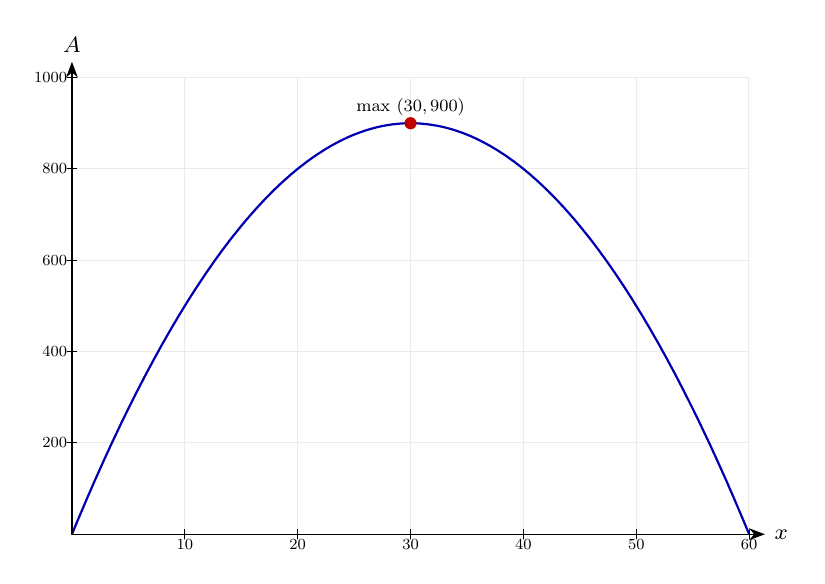
\begin{tikzpicture}[>={Stealth[length=2mm]},font=\footnotesize,line cap=round,line join=round]
\begin{scope}
\clip (0,0) rectangle (8.6,5.8);
\draw[gray!16] (0,0) grid[xstep=1.433,ystep=1.16] (8.6,5.8);
\draw[blue!70!black,thick] (0,0) -- (0.031,0.074) -- (0.061,0.148) -- (0.092,0.221) -- (0.123,0.294) -- (0.154,0.366) -- (0.184,0.438) -- (0.215,0.509) -- (0.246,0.58) -- (0.276,0.65) -- (0.307,0.719) -- (0.338,0.788) -- (0.369,0.857) -- (0.399,0.924) -- (0.43,0.992) -- (0.461,1.059) -- (0.491,1.125) -- (0.522,1.191) -- (0.553,1.256) -- (0.584,1.321) -- (0.614,1.385) -- (0.645,1.449) -- (0.676,1.512) -- (0.706,1.574) -- (0.737,1.636) -- (0.768,1.698) -- (0.799,1.759) -- (0.829,1.819) -- (0.86,1.879) -- (0.891,1.939) -- (0.921,1.997) -- (0.952,2.056) -- (0.983,2.114) -- (1.014,2.171) -- (1.044,2.228) -- (1.075,2.284) -- (1.106,2.339) -- (1.136,2.395) -- (1.167,2.449) -- (1.198,2.503) -- (1.229,2.557) -- (1.259,2.61) -- (1.29,2.662) -- (1.321,2.714) -- (1.351,2.766) -- (1.382,2.816) -- (1.413,2.867) -- (1.444,2.917) -- (1.474,2.966) -- (1.505,3.015) -- (1.536,3.063) -- (1.566,3.11) -- (1.597,3.158) -- (1.628,3.204) -- (1.659,3.25) -- (1.689,3.296) -- (1.72,3.341) -- (1.751,3.385) -- (1.781,3.429) -- (1.812,3.473) -- (1.843,3.516) -- (1.874,3.558) -- (1.904,3.6) -- (1.935,3.641) -- (1.966,3.682) -- (1.996,3.722) -- (2.027,3.762) -- (2.058,3.801) -- (2.089,3.839) -- (2.119,3.877) -- (2.15,3.915) -- (2.181,3.952) -- (2.211,3.989) -- (2.242,4.024) -- (2.273,4.06) -- (2.304,4.095) -- (2.334,4.129) -- (2.365,4.163) -- (2.396,4.196) -- (2.426,4.229) -- (2.457,4.261) -- (2.488,4.293) -- (2.519,4.324) -- (2.549,4.355) -- (2.58,4.385) -- (2.611,4.414) -- (2.641,4.443) -- (2.672,4.472) -- (2.703,4.5) -- (2.734,4.527) -- (2.764,4.554) -- (2.795,4.581) -- (2.826,4.606) -- (2.856,4.632) -- (2.887,4.656) -- (2.918,4.681) -- (2.949,4.704) -- (2.979,4.728) -- (3.01,4.75) -- (3.041,4.772) -- (3.071,4.794) -- (3.102,4.815) -- (3.133,4.835) -- (3.164,4.855) -- (3.194,4.875) -- (3.225,4.894) -- (3.256,4.912) -- (3.286,4.93) -- (3.317,4.947) -- (3.348,4.964) -- (3.379,4.98) -- (3.409,4.996) -- (3.44,5.011) -- (3.471,5.026) -- (3.501,5.04) -- (3.532,5.054) -- (3.563,5.067) -- (3.594,5.079) -- (3.624,5.091) -- (3.655,5.103) -- (3.686,5.113) -- (3.716,5.124) -- (3.747,5.134) -- (3.778,5.143) -- (3.809,5.152) -- (3.839,5.16) -- (3.87,5.168) -- (3.901,5.175) -- (3.931,5.182) -- (3.962,5.188) -- (3.993,5.193) -- (4.024,5.198) -- (4.054,5.203) -- (4.085,5.207) -- (4.116,5.21) -- (4.146,5.213) -- (4.177,5.216) -- (4.208,5.218) -- (4.239,5.219) -- (4.269,5.22) -- (4.3,5.22) -- (4.331,5.22) -- (4.361,5.219) -- (4.392,5.218) -- (4.423,5.216) -- (4.454,5.213) -- (4.484,5.21) -- (4.515,5.207) -- (4.546,5.203) -- (4.576,5.198) -- (4.607,5.193) -- (4.638,5.188) -- (4.669,5.182) -- (4.699,5.175) -- (4.73,5.168) -- (4.761,5.16) -- (4.791,5.152) -- (4.822,5.143) -- (4.853,5.134) -- (4.884,5.124) -- (4.914,5.113) -- (4.945,5.103) -- (4.976,5.091) -- (5.006,5.079) -- (5.037,5.067) -- (5.068,5.054) -- (5.099,5.04) -- (5.129,5.026) -- (5.16,5.011) -- (5.191,4.996) -- (5.221,4.98) -- (5.252,4.964) -- (5.283,4.947) -- (5.314,4.93) -- (5.344,4.912) -- (5.375,4.894) -- (5.406,4.875) -- (5.436,4.855) -- (5.467,4.835) -- (5.498,4.815) -- (5.529,4.794) -- (5.559,4.772) -- (5.59,4.75) -- (5.621,4.728) -- (5.651,4.704) -- (5.682,4.681) -- (5.713,4.656) -- (5.744,4.632) -- (5.774,4.606) -- (5.805,4.581) -- (5.836,4.554) -- (5.866,4.527) -- (5.897,4.5) -- (5.928,4.472) -- (5.959,4.443) -- (5.989,4.414) -- (6.02,4.385) -- (6.051,4.355) -- (6.081,4.324) -- (6.112,4.293) -- (6.143,4.261) -- (6.174,4.229) -- (6.204,4.196) -- (6.235,4.163) -- (6.266,4.129) -- (6.296,4.095) -- (6.327,4.06) -- (6.358,4.024) -- (6.389,3.989) -- (6.419,3.952) -- (6.45,3.915) -- (6.481,3.877) -- (6.511,3.839) -- (6.542,3.801) -- (6.573,3.762) -- (6.604,3.722) -- (6.634,3.682) -- (6.665,3.641) -- (6.696,3.6) -- (6.726,3.558) -- (6.757,3.516) -- (6.788,3.473) -- (6.819,3.429) -- (6.849,3.385) -- (6.88,3.341) -- (6.911,3.296) -- (6.941,3.25) -- (6.972,3.204) -- (7.003,3.158) -- (7.034,3.11) -- (7.064,3.063) -- (7.095,3.015) -- (7.126,2.966) -- (7.156,2.917) -- (7.187,2.867) -- (7.218,2.816) -- (7.249,2.766) -- (7.279,2.714) -- (7.31,2.662) -- (7.341,2.61) -- (7.371,2.557) -- (7.402,2.503) -- (7.433,2.449) -- (7.464,2.395) -- (7.494,2.339) -- (7.525,2.284) -- (7.556,2.228) -- (7.586,2.171) -- (7.617,2.114) -- (7.648,2.056) -- (7.679,1.997) -- (7.709,1.939) -- (7.74,1.879) -- (7.771,1.819) -- (7.801,1.759) -- (7.832,1.698) -- (7.863,1.636) -- (7.894,1.574) -- (7.924,1.512) -- (7.955,1.449) -- (7.986,1.385) -- (8.016,1.321) -- (8.047,1.256) -- (8.078,1.191) -- (8.109,1.125) -- (8.139,1.059) -- (8.17,0.992) -- (8.201,0.924) -- (8.231,0.857) -- (8.262,0.788) -- (8.293,0.719) -- (8.324,0.65) -- (8.354,0.58) -- (8.385,0.509) -- (8.416,0.438) -- (8.446,0.366) -- (8.477,0.294) -- (8.508,0.221) -- (8.539,0.148) -- (8.569,0.074) -- (8.6,0);
\end{scope}
\draw[->] (0,0) -- (8.8,0) node[right]{$x$};
\draw[->] (0,0) -- (0,6) node[above]{$A$};
\draw (1.433,-0.06) -- (1.433,0.06) node[below=1pt,scale=0.7]{$10$};
\draw (2.867,-0.06) -- (2.867,0.06) node[below=1pt,scale=0.7]{$20$};
\draw (4.3,-0.06) -- (4.3,0.06) node[below=1pt,scale=0.7]{$30$};
\draw (5.733,-0.06) -- (5.733,0.06) node[below=1pt,scale=0.7]{$40$};
\draw (7.167,-0.06) -- (7.167,0.06) node[below=1pt,scale=0.7]{$50$};
\draw (8.6,-0.06) -- (8.6,0.06) node[below=1pt,scale=0.7]{$60$};
\draw (-0.06,1.16) -- (0.06,1.16) node[left=1pt,scale=0.7]{$200$};
\draw (-0.06,2.32) -- (0.06,2.32) node[left=1pt,scale=0.7]{$400$};
\draw (-0.06,3.48) -- (0.06,3.48) node[left=1pt,scale=0.7]{$600$};
\draw (-0.06,4.64) -- (0.06,4.64) node[left=1pt,scale=0.7]{$800$};
\draw (-0.06,5.8) -- (0.06,5.8) node[left=1pt,scale=0.7]{$1000$};
\fill[red!75!black] (4.3,5.22) circle (2.2pt);
\node[above,scale=0.78] at (4.3,5.22) {max $(30,900)$};
\end{tikzpicture}
}
\end{center}
\small The model plotted against its variable, with the key point(s) marked.\normalsize

\medskip\hrule

\section*{Real-Life Problems 14\quad\small\texttt{(d5-014)}}
\addcontentsline{toc}{section}{Real-Life Problems 14 (d5-014)}
\textit{Difficulty: Foundation \quad\textbar\quad Marks: 6}

\question{A child cuts equal squares of side \( x \) cm from each corner of a \( 30 \times 30 \) cm piece of card and folds the sides up to make an open box. (a) Show that the volume of the box is \( V = x(30 - 2x)^2 \). (b) Find the value of \( x \) that maximises the volume.}

\textbf{Worked solution.}

\textit{Step 1: (a) After cutting, the base has side \( (30 - 2x) \) cm and the height is \( x \) cm.}
\[\begin{gathered}
V = x(30 - 2x)^2
\end{gathered}\]
Volume = base area $\times$ height; the base is a square of side \( (30 - 2x) \).

\textit{Step 2: (b) Expand.}
\[\begin{gathered}
V = x(900 - 120x + 4x^2) = 900x - 120x^2 + 4x^3
\end{gathered}\]
Expand \( (30-2x)^2 \) first, then multiply by \( x \).

\textit{Step 3: Differentiate.}
\[\begin{gathered}
\frac{\mathrm{d}V}{\mathrm{d}x} = 900 - 240x + 12x^2
\end{gathered}\]
Power rule.

\textit{Step 4: Set to zero and simplify.}
\[\begin{gathered}
12x^2 - 240x + 900 = 0 \implies x^2 - 20x + 75 = 0 \implies (x-5)(x-15) = 0
\end{gathered}\]
Divide by 12, then factorise.

\textit{Step 5: Identify the valid solution.}
\[\begin{gathered}
x = 5 \text{ or } x = 15; \quad x = 15 \text{ gives } (30 - 30) = 0 \text{, so reject}
\end{gathered}\]
\( x = 15 \) gives zero base length --- not a valid box. \( x = 5 \) gives a real box.

\textit{Step 6: Confirm maximum at \( x = 5 \).}
\[\begin{gathered}
\frac{\mathrm{d}^2V}{\mathrm{d}x^2} = -240 + 24x; \quad x=5: -240+120 = -120 < 0 \Rightarrow \text{maximum}
\end{gathered}\]
Negative second derivative confirms a maximum.

\begin{answerbox}
\textbf{Final answer:}\quad (a) Shown. \\[3pt]  (b) \(\displaystyle  x = 5 \) cm maximises the volume.
\end{answerbox}
\textbf{Diagram.}

\begin{center}
\resizebox{\ifdim\width>\linewidth \linewidth\else \width\fi}{!}{%
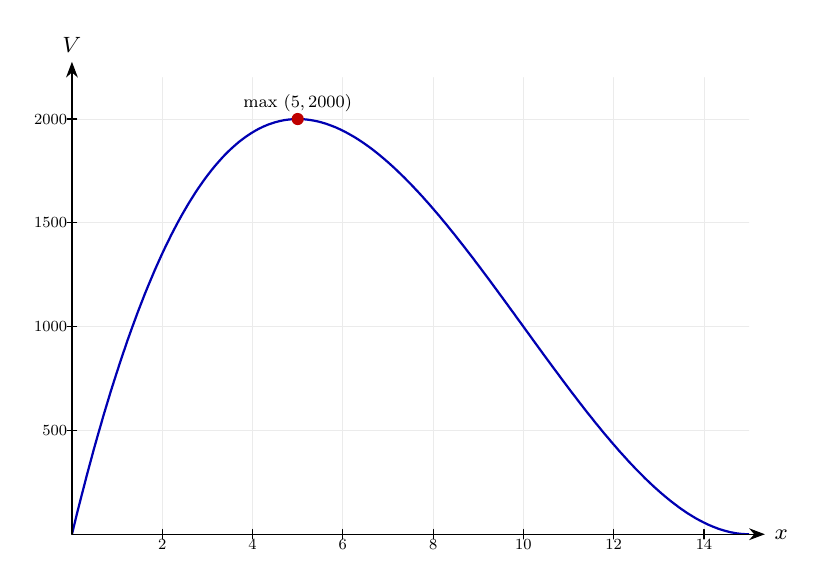
\begin{tikzpicture}[>={Stealth[length=2mm]},font=\footnotesize,line cap=round,line join=round]
\begin{scope}
\clip (0,0) rectangle (8.6,5.8);
\draw[gray!16] (0,0) grid[xstep=1.147,ystep=1.318] (8.6,5.8);
\draw[blue!70!black,thick] (0,0) -- (0.031,0.126) -- (0.061,0.251) -- (0.092,0.373) -- (0.123,0.494) -- (0.154,0.613) -- (0.184,0.73) -- (0.215,0.846) -- (0.246,0.96) -- (0.276,1.072) -- (0.307,1.182) -- (0.338,1.291) -- (0.369,1.397) -- (0.399,1.503) -- (0.43,1.606) -- (0.461,1.708) -- (0.491,1.808) -- (0.522,1.906) -- (0.553,2.003) -- (0.584,2.098) -- (0.614,2.192) -- (0.645,2.284) -- (0.676,2.374) -- (0.706,2.463) -- (0.737,2.55) -- (0.768,2.636) -- (0.799,2.72) -- (0.829,2.802) -- (0.86,2.883) -- (0.891,2.962) -- (0.921,3.04) -- (0.952,3.116) -- (0.983,3.191) -- (1.014,3.264) -- (1.044,3.336) -- (1.075,3.406) -- (1.106,3.475) -- (1.136,3.542) -- (1.167,3.608) -- (1.198,3.673) -- (1.229,3.735) -- (1.259,3.797) -- (1.29,3.857) -- (1.321,3.916) -- (1.351,3.973) -- (1.382,4.029) -- (1.413,4.084) -- (1.444,4.137) -- (1.474,4.189) -- (1.505,4.239) -- (1.536,4.288) -- (1.566,4.336) -- (1.597,4.383) -- (1.628,4.428) -- (1.659,4.472) -- (1.689,4.514) -- (1.72,4.556) -- (1.751,4.596) -- (1.781,4.634) -- (1.812,4.672) -- (1.843,4.708) -- (1.874,4.743) -- (1.904,4.777) -- (1.935,4.81) -- (1.966,4.841) -- (1.996,4.871) -- (2.027,4.9) -- (2.058,4.928) -- (2.089,4.955) -- (2.119,4.981) -- (2.15,5.005) -- (2.181,5.028) -- (2.211,5.05) -- (2.242,5.071) -- (2.273,5.091) -- (2.304,5.11) -- (2.334,5.128) -- (2.365,5.145) -- (2.396,5.16) -- (2.426,5.175) -- (2.457,5.188) -- (2.488,5.201) -- (2.519,5.212) -- (2.549,5.222) -- (2.58,5.232) -- (2.611,5.24) -- (2.641,5.248) -- (2.672,5.254) -- (2.703,5.26) -- (2.734,5.264) -- (2.764,5.268) -- (2.795,5.27) -- (2.826,5.272) -- (2.856,5.273) -- (2.887,5.273) -- (2.918,5.271) -- (2.949,5.27) -- (2.979,5.267) -- (3.01,5.263) -- (3.041,5.258) -- (3.071,5.253) -- (3.102,5.247) -- (3.133,5.24) -- (3.164,5.232) -- (3.194,5.223) -- (3.225,5.214) -- (3.256,5.203) -- (3.286,5.192) -- (3.317,5.18) -- (3.348,5.168) -- (3.379,5.154) -- (3.409,5.14) -- (3.44,5.125) -- (3.471,5.109) -- (3.501,5.093) -- (3.532,5.076) -- (3.563,5.058) -- (3.594,5.04) -- (3.624,5.021) -- (3.655,5.001) -- (3.686,4.981) -- (3.716,4.96) -- (3.747,4.938) -- (3.778,4.916) -- (3.809,4.893) -- (3.839,4.869) -- (3.87,4.845) -- (3.901,4.82) -- (3.931,4.795) -- (3.962,4.769) -- (3.993,4.742) -- (4.024,4.715) -- (4.054,4.688) -- (4.085,4.66) -- (4.116,4.631) -- (4.146,4.602) -- (4.177,4.572) -- (4.208,4.542) -- (4.239,4.511) -- (4.269,4.48) -- (4.3,4.449) -- (4.331,4.417) -- (4.361,4.384) -- (4.392,4.352) -- (4.423,4.318) -- (4.454,4.285) -- (4.484,4.25) -- (4.515,4.216) -- (4.546,4.181) -- (4.576,4.146) -- (4.607,4.11) -- (4.638,4.074) -- (4.669,4.038) -- (4.699,4.001) -- (4.73,3.964) -- (4.761,3.927) -- (4.791,3.889) -- (4.822,3.851) -- (4.853,3.813) -- (4.884,3.774) -- (4.914,3.735) -- (4.945,3.696) -- (4.976,3.657) -- (5.006,3.618) -- (5.037,3.578) -- (5.068,3.538) -- (5.099,3.498) -- (5.129,3.457) -- (5.16,3.417) -- (5.191,3.376) -- (5.221,3.335) -- (5.252,3.294) -- (5.283,3.253) -- (5.314,3.211) -- (5.344,3.17) -- (5.375,3.128) -- (5.406,3.086) -- (5.436,3.044) -- (5.467,3.003) -- (5.498,2.96) -- (5.529,2.918) -- (5.559,2.876) -- (5.59,2.834) -- (5.621,2.792) -- (5.651,2.749) -- (5.682,2.707) -- (5.713,2.665) -- (5.744,2.622) -- (5.774,2.58) -- (5.805,2.538) -- (5.836,2.495) -- (5.866,2.453) -- (5.897,2.411) -- (5.928,2.368) -- (5.959,2.326) -- (5.989,2.284) -- (6.02,2.242) -- (6.051,2.2) -- (6.081,2.159) -- (6.112,2.117) -- (6.143,2.075) -- (6.174,2.034) -- (6.204,1.993) -- (6.235,1.951) -- (6.266,1.91) -- (6.296,1.87) -- (6.327,1.829) -- (6.358,1.788) -- (6.389,1.748) -- (6.419,1.708) -- (6.45,1.668) -- (6.481,1.629) -- (6.511,1.589) -- (6.542,1.55) -- (6.573,1.511) -- (6.604,1.473) -- (6.634,1.434) -- (6.665,1.396) -- (6.696,1.359) -- (6.726,1.321) -- (6.757,1.284) -- (6.788,1.247) -- (6.819,1.211) -- (6.849,1.175) -- (6.88,1.139) -- (6.911,1.104) -- (6.941,1.068) -- (6.972,1.034) -- (7.003,1) -- (7.034,0.966) -- (7.064,0.932) -- (7.095,0.899) -- (7.126,0.867) -- (7.156,0.834) -- (7.187,0.803) -- (7.218,0.772) -- (7.249,0.741) -- (7.279,0.71) -- (7.31,0.681) -- (7.341,0.651) -- (7.371,0.623) -- (7.402,0.594) -- (7.433,0.567) -- (7.464,0.539) -- (7.494,0.513) -- (7.525,0.487) -- (7.556,0.461) -- (7.586,0.436) -- (7.617,0.412) -- (7.648,0.388) -- (7.679,0.365) -- (7.709,0.342) -- (7.74,0.32) -- (7.771,0.299) -- (7.801,0.278) -- (7.832,0.258) -- (7.863,0.239) -- (7.894,0.22) -- (7.924,0.202) -- (7.955,0.185) -- (7.986,0.169) -- (8.016,0.153) -- (8.047,0.138) -- (8.078,0.123) -- (8.109,0.11) -- (8.139,0.097) -- (8.17,0.085) -- (8.201,0.073) -- (8.231,0.063) -- (8.262,0.053) -- (8.293,0.044) -- (8.324,0.036) -- (8.354,0.028) -- (8.385,0.022) -- (8.416,0.016) -- (8.446,0.011) -- (8.477,0.007) -- (8.508,0.004) -- (8.539,0.002) -- (8.569,0) -- (8.6,0);
\end{scope}
\draw[->] (0,0) -- (8.8,0) node[right]{$x$};
\draw[->] (0,0) -- (0,6) node[above]{$V$};
\draw (1.147,-0.06) -- (1.147,0.06) node[below=1pt,scale=0.7]{$2$};
\draw (2.293,-0.06) -- (2.293,0.06) node[below=1pt,scale=0.7]{$4$};
\draw (3.44,-0.06) -- (3.44,0.06) node[below=1pt,scale=0.7]{$6$};
\draw (4.587,-0.06) -- (4.587,0.06) node[below=1pt,scale=0.7]{$8$};
\draw (5.733,-0.06) -- (5.733,0.06) node[below=1pt,scale=0.7]{$10$};
\draw (6.88,-0.06) -- (6.88,0.06) node[below=1pt,scale=0.7]{$12$};
\draw (8.027,-0.06) -- (8.027,0.06) node[below=1pt,scale=0.7]{$14$};
\draw (-0.06,1.318) -- (0.06,1.318) node[left=1pt,scale=0.7]{$500$};
\draw (-0.06,2.636) -- (0.06,2.636) node[left=1pt,scale=0.7]{$1000$};
\draw (-0.06,3.955) -- (0.06,3.955) node[left=1pt,scale=0.7]{$1500$};
\draw (-0.06,5.273) -- (0.06,5.273) node[left=1pt,scale=0.7]{$2000$};
\fill[red!75!black] (2.867,5.273) circle (2.2pt);
\node[above,scale=0.78] at (2.867,5.273) {max $(5,2000)$};
\end{tikzpicture}
}
\end{center}
\small The model plotted against its variable, with the key point(s) marked.\normalsize

\medskip\hrule

\section*{Real-Life Problems 15\quad\small\texttt{(d5-015)}}
\addcontentsline{toc}{section}{Real-Life Problems 15 (d5-015)}
\textit{Difficulty: Foundation \quad\textbar\quad Marks: 6}

\question{A closed cylindrical can has radius \( r \) cm and height \( h \) cm. Its volume is \( 250\pi \) cm\(^3\). (a) Show that the total surface area is \( A = 2\pi r^2 + \dfrac{500\pi}{r} \). (b) Find the value of \( r \) that minimises \( A \).}

\textbf{Worked solution.}

\textit{Step 1: (a) Volume: \( \pi r^2 h = 250\pi \).}
\[\begin{gathered}
h = \frac{250}{r^2}
\end{gathered}\]
Rearrange to express \( h \) in terms of \( r \).

\textit{Step 2: Surface area: two circles + curved surface.}
\[\begin{gathered}
A = 2\pi r^2 + 2\pi r h = 2\pi r^2 + 2\pi r \cdot \frac{250}{r^2} = 2\pi r^2 + \frac{500\pi}{r}
\end{gathered}\]
Substitute \( h = \dfrac{250}{r^2} \) into the surface area formula.

\textit{Step 3: (b) Rewrite and differentiate.}
\[\begin{gathered}
A = 2\pi r^2 + 500\pi r^{-1} \implies \frac{\mathrm{d}A}{\mathrm{d}r} = 4\pi r - \frac{500\pi}{r^2}
\end{gathered}\]
Convert \( \dfrac{1}{r} \) to \( r^{-1} \) before differentiating.

\textit{Step 4: Set to zero.}
\[\begin{gathered}
4\pi r = \frac{500\pi}{r^2} \implies 4r^3 = 500 \implies r^3 = 125 \implies r = 5 \text{ cm}
\end{gathered}\]
Multiply both sides by \( r^2 \) and solve for \( r \).

\textit{Step 5: Confirm minimum.}
\[\begin{gathered}
\frac{\mathrm{d}^2A}{\mathrm{d}r^2} = 4\pi + \frac{1000\pi}{r^3}; \quad r=5: 4\pi + 8\pi = 12\pi > 0 \Rightarrow \text{minimum}
\end{gathered}\]
Positive second derivative confirms a minimum.

\begin{answerbox}
\textbf{Final answer:}\quad (a) Shown. \\[3pt]  (b) \(\displaystyle  r = 5 \) cm
\end{answerbox}
\textbf{Diagram.}

\begin{center}
\resizebox{\ifdim\width>\linewidth \linewidth\else \width\fi}{!}{%
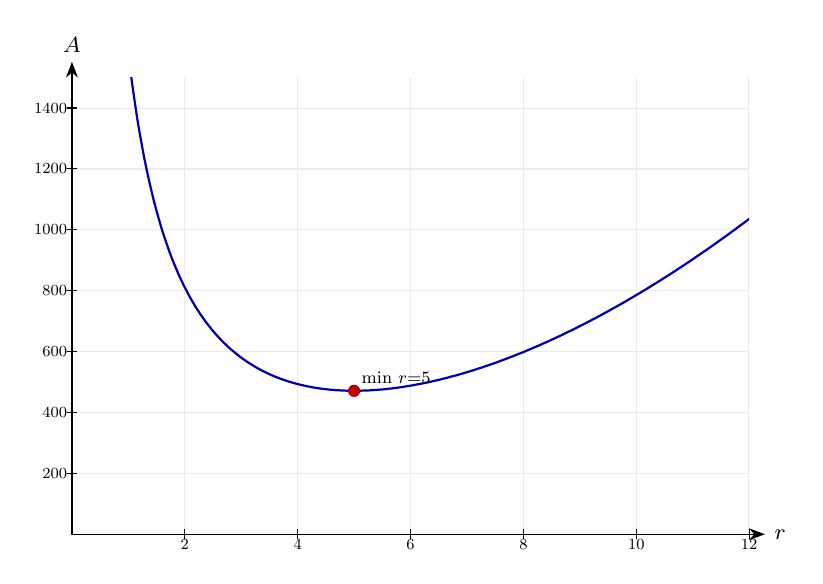
\begin{tikzpicture}[>={Stealth[length=2mm]},font=\footnotesize,line cap=round,line join=round]
\begin{scope}
\clip (0,0) rectangle (8.6,5.8);
\draw[gray!16] (0,0) grid[xstep=1.433,ystep=0.773] (8.6,5.8);
\draw[blue!70!black,thick] (0.031,11.6) -- (0.061,11.6) -- (0.092,11.6) -- (0.123,11.6) -- (0.154,11.6) -- (0.184,11.6) -- (0.215,11.6) -- (0.246,11.6) -- (0.276,11.6) -- (0.307,11.6) -- (0.338,11.6) -- (0.369,11.6) -- (0.399,10.909) -- (0.43,10.132) -- (0.461,9.458) -- (0.491,8.869) -- (0.522,8.349) -- (0.553,7.888) -- (0.584,7.475) -- (0.614,7.104) -- (0.645,6.768) -- (0.676,6.463) -- (0.706,6.185) -- (0.737,5.931) -- (0.768,5.697) -- (0.799,5.481) -- (0.829,5.281) -- (0.86,5.096) -- (0.891,4.924) -- (0.921,4.764) -- (0.952,4.615) -- (0.983,4.474) -- (1.014,4.343) -- (1.044,4.22) -- (1.075,4.104) -- (1.106,3.995) -- (1.136,3.891) -- (1.167,3.794) -- (1.198,3.702) -- (1.229,3.614) -- (1.259,3.532) -- (1.29,3.453) -- (1.321,3.378) -- (1.351,3.307) -- (1.382,3.24) -- (1.413,3.175) -- (1.444,3.114) -- (1.474,3.055) -- (1.505,2.999) -- (1.536,2.946) -- (1.566,2.895) -- (1.597,2.846) -- (1.628,2.799) -- (1.659,2.755) -- (1.689,2.712) -- (1.72,2.671) -- (1.751,2.631) -- (1.781,2.594) -- (1.812,2.557) -- (1.843,2.523) -- (1.874,2.489) -- (1.904,2.457) -- (1.935,2.427) -- (1.966,2.397) -- (1.996,2.369) -- (2.027,2.342) -- (2.058,2.316) -- (2.089,2.29) -- (2.119,2.266) -- (2.15,2.243) -- (2.181,2.221) -- (2.211,2.2) -- (2.242,2.179) -- (2.273,2.16) -- (2.304,2.141) -- (2.334,2.122) -- (2.365,2.105) -- (2.396,2.088) -- (2.426,2.072) -- (2.457,2.057) -- (2.488,2.042) -- (2.519,2.028) -- (2.549,2.015) -- (2.58,2.002) -- (2.611,1.99) -- (2.641,1.978) -- (2.672,1.967) -- (2.703,1.956) -- (2.734,1.946) -- (2.764,1.936) -- (2.795,1.927) -- (2.826,1.918) -- (2.856,1.91) -- (2.887,1.902) -- (2.918,1.895) -- (2.949,1.888) -- (2.979,1.881) -- (3.01,1.875) -- (3.041,1.869) -- (3.071,1.863) -- (3.102,1.858) -- (3.133,1.854) -- (3.164,1.849) -- (3.194,1.845) -- (3.225,1.842) -- (3.256,1.838) -- (3.286,1.835) -- (3.317,1.833) -- (3.348,1.83) -- (3.379,1.828) -- (3.409,1.827) -- (3.44,1.825) -- (3.471,1.824) -- (3.501,1.823) -- (3.532,1.822) -- (3.563,1.822) -- (3.594,1.822) -- (3.624,1.822) -- (3.655,1.823) -- (3.686,1.824) -- (3.716,1.825) -- (3.747,1.826) -- (3.778,1.827) -- (3.809,1.829) -- (3.839,1.831) -- (3.87,1.833) -- (3.901,1.836) -- (3.931,1.838) -- (3.962,1.841) -- (3.993,1.844) -- (4.024,1.848) -- (4.054,1.851) -- (4.085,1.855) -- (4.116,1.859) -- (4.146,1.863) -- (4.177,1.867) -- (4.208,1.872) -- (4.239,1.877) -- (4.269,1.882) -- (4.3,1.887) -- (4.331,1.892) -- (4.361,1.898) -- (4.392,1.904) -- (4.423,1.909) -- (4.454,1.916) -- (4.484,1.922) -- (4.515,1.928) -- (4.546,1.935) -- (4.576,1.942) -- (4.607,1.949) -- (4.638,1.956) -- (4.669,1.963) -- (4.699,1.971) -- (4.73,1.979) -- (4.761,1.986) -- (4.791,1.994) -- (4.822,2.003) -- (4.853,2.011) -- (4.884,2.019) -- (4.914,2.028) -- (4.945,2.037) -- (4.976,2.046) -- (5.006,2.055) -- (5.037,2.064) -- (5.068,2.074) -- (5.099,2.083) -- (5.129,2.093) -- (5.16,2.103) -- (5.191,2.113) -- (5.221,2.123) -- (5.252,2.134) -- (5.283,2.144) -- (5.314,2.155) -- (5.344,2.166) -- (5.375,2.176) -- (5.406,2.187) -- (5.436,2.199) -- (5.467,2.21) -- (5.498,2.222) -- (5.529,2.233) -- (5.559,2.245) -- (5.59,2.257) -- (5.621,2.269) -- (5.651,2.281) -- (5.682,2.293) -- (5.713,2.306) -- (5.744,2.318) -- (5.774,2.331) -- (5.805,2.344) -- (5.836,2.357) -- (5.866,2.37) -- (5.897,2.383) -- (5.928,2.396) -- (5.959,2.41) -- (5.989,2.424) -- (6.02,2.437) -- (6.051,2.451) -- (6.081,2.465) -- (6.112,2.479) -- (6.143,2.494) -- (6.174,2.508) -- (6.204,2.522) -- (6.235,2.537) -- (6.266,2.552) -- (6.296,2.567) -- (6.327,2.582) -- (6.358,2.597) -- (6.389,2.612) -- (6.419,2.627) -- (6.45,2.643) -- (6.481,2.658) -- (6.511,2.674) -- (6.542,2.69) -- (6.573,2.706) -- (6.604,2.722) -- (6.634,2.738) -- (6.665,2.754) -- (6.696,2.771) -- (6.726,2.787) -- (6.757,2.804) -- (6.788,2.821) -- (6.819,2.838) -- (6.849,2.855) -- (6.88,2.872) -- (6.911,2.889) -- (6.941,2.906) -- (6.972,2.924) -- (7.003,2.941) -- (7.034,2.959) -- (7.064,2.977) -- (7.095,2.995) -- (7.126,3.013) -- (7.156,3.031) -- (7.187,3.049) -- (7.218,3.067) -- (7.249,3.086) -- (7.279,3.104) -- (7.31,3.123) -- (7.341,3.142) -- (7.371,3.161) -- (7.402,3.18) -- (7.433,3.199) -- (7.464,3.218) -- (7.494,3.238) -- (7.525,3.257) -- (7.556,3.277) -- (7.586,3.296) -- (7.617,3.316) -- (7.648,3.336) -- (7.679,3.356) -- (7.709,3.376) -- (7.74,3.396) -- (7.771,3.416) -- (7.801,3.437) -- (7.832,3.457) -- (7.863,3.478) -- (7.894,3.499) -- (7.924,3.52) -- (7.955,3.541) -- (7.986,3.562) -- (8.016,3.583) -- (8.047,3.604) -- (8.078,3.625) -- (8.109,3.647) -- (8.139,3.668) -- (8.17,3.69) -- (8.201,3.712) -- (8.231,3.734) -- (8.262,3.756) -- (8.293,3.778) -- (8.324,3.8) -- (8.354,3.822) -- (8.385,3.845) -- (8.416,3.867) -- (8.446,3.89) -- (8.477,3.913) -- (8.508,3.936) -- (8.539,3.958) -- (8.569,3.981) -- (8.6,4.005);
\end{scope}
\draw[->] (0,0) -- (8.8,0) node[right]{$r$};
\draw[->] (0,0) -- (0,6) node[above]{$A$};
\draw (1.433,-0.06) -- (1.433,0.06) node[below=1pt,scale=0.7]{$2$};
\draw (2.867,-0.06) -- (2.867,0.06) node[below=1pt,scale=0.7]{$4$};
\draw (4.3,-0.06) -- (4.3,0.06) node[below=1pt,scale=0.7]{$6$};
\draw (5.733,-0.06) -- (5.733,0.06) node[below=1pt,scale=0.7]{$8$};
\draw (7.167,-0.06) -- (7.167,0.06) node[below=1pt,scale=0.7]{$10$};
\draw (8.6,-0.06) -- (8.6,0.06) node[below=1pt,scale=0.7]{$12$};
\draw (-0.06,0.773) -- (0.06,0.773) node[left=1pt,scale=0.7]{$200$};
\draw (-0.06,1.547) -- (0.06,1.547) node[left=1pt,scale=0.7]{$400$};
\draw (-0.06,2.32) -- (0.06,2.32) node[left=1pt,scale=0.7]{$600$};
\draw (-0.06,3.093) -- (0.06,3.093) node[left=1pt,scale=0.7]{$800$};
\draw (-0.06,3.867) -- (0.06,3.867) node[left=1pt,scale=0.7]{$1000$};
\draw (-0.06,4.64) -- (0.06,4.64) node[left=1pt,scale=0.7]{$1200$};
\draw (-0.06,5.413) -- (0.06,5.413) node[left=1pt,scale=0.7]{$1400$};
\fill[red!75!black] (3.583,1.821) circle (2.2pt);
\node[above right,scale=0.78] at (3.583,1.821) {min $r{=}5$};
\end{tikzpicture}
}
\end{center}
\small The model plotted against its variable, with the key point(s) marked.\normalsize

\medskip\hrule

\section*{Real-Life Problems 16\quad\small\texttt{(d5-016)}}
\addcontentsline{toc}{section}{Real-Life Problems 16 (d5-016)}
\textit{Difficulty: Foundation \quad\textbar\quad Marks: 5}

\question{A particle moves so that its velocity at time \( t \) seconds is \( v = 3t^2 - 12t + 9 \) ms\(^{-1}\). (a) Find the acceleration function. (b) Find the acceleration when the particle has zero velocity. (c) Find the minimum velocity.}

\textbf{Worked solution.}

\textit{Step 1: (a) Differentiate \( v \) with respect to \( t \).}
\[\begin{gathered}
a = \frac{\mathrm{d}v}{\mathrm{d}t} = 6t - 12
\end{gathered}\]
Acceleration is the derivative of velocity.

\textit{Step 2: (b) Find when \( v = 0 \).}
\[\begin{gathered}
3t^2 - 12t + 9 = 0 \implies (t-1)(t-3) = 0 \implies t = 1 \text{ or } t = 3
\end{gathered}\]
Divide by 3 and factorise.

\textit{Step 3: Acceleration at \( t = 1 \) and \( t = 3 \).}
\[\begin{gathered}
a(1) = 6-12 = -6 \text{ ms}^{-2}; \quad a(3) = 18-12 = 6 \text{ ms}^{-2}
\end{gathered}\]
Substitute each \( t \) into \( a \).

\textit{Step 4: (c) Minimum velocity: set \( \dfrac{\mathrm{d}v}{\mathrm{d}t} = 0 \).}
\[\begin{gathered}
6t - 12 = 0 \implies t = 2; \quad v(2) = 12 - 24 + 9 = -3 \text{ ms}^{-1}
\end{gathered}\]
Find the turning point of \( v \). The negative value means the particle moves in reverse.

\begin{answerbox}
\textbf{Final answer:}\quad (a) \(\displaystyle  a = 6t - 12 \) \\[3pt]  (b) \(\displaystyle  -6 \text{ ms}^{-2} \) at \(\displaystyle  t=1 \); \(\displaystyle  6 \text{ ms}^{-2} \) at \(\displaystyle  t=3 \) \\[3pt]  (c) Minimum velocity \(\displaystyle  = -3 \text{ ms}^{-1} \)
\end{answerbox}
\textbf{Diagram.}

\begin{center}
\resizebox{\ifdim\width>\linewidth \linewidth\else \width\fi}{!}{%
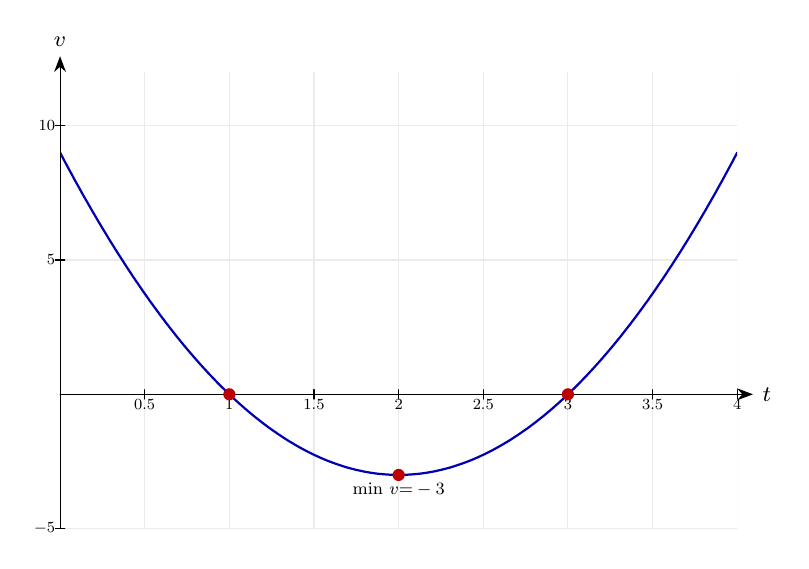
\begin{tikzpicture}[>={Stealth[length=2mm]},font=\footnotesize,line cap=round,line join=round]
\begin{scope}
\clip (0,0) rectangle (8.6,5.8);
\draw[gray!16] (0,0) grid[xstep=1.075,ystep=1.706] (8.6,5.8);
\draw[blue!70!black,thick] (0,4.776) -- (0.031,4.718) -- (0.061,4.66) -- (0.092,4.603) -- (0.123,4.546) -- (0.154,4.489) -- (0.184,4.433) -- (0.215,4.377) -- (0.246,4.322) -- (0.276,4.267) -- (0.307,4.212) -- (0.338,4.158) -- (0.369,4.105) -- (0.399,4.051) -- (0.43,3.999) -- (0.461,3.946) -- (0.491,3.894) -- (0.522,3.843) -- (0.553,3.791) -- (0.584,3.741) -- (0.614,3.69) -- (0.645,3.64) -- (0.676,3.591) -- (0.706,3.542) -- (0.737,3.493) -- (0.768,3.445) -- (0.799,3.397) -- (0.829,3.35) -- (0.86,3.303) -- (0.891,3.256) -- (0.921,3.21) -- (0.952,3.164) -- (0.983,3.119) -- (1.014,3.074) -- (1.044,3.029) -- (1.075,2.985) -- (1.106,2.942) -- (1.136,2.898) -- (1.167,2.856) -- (1.198,2.813) -- (1.229,2.771) -- (1.259,2.73) -- (1.29,2.688) -- (1.321,2.648) -- (1.351,2.607) -- (1.382,2.568) -- (1.413,2.528) -- (1.444,2.489) -- (1.474,2.45) -- (1.505,2.412) -- (1.536,2.374) -- (1.566,2.337) -- (1.597,2.3) -- (1.628,2.263) -- (1.659,2.227) -- (1.689,2.192) -- (1.72,2.156) -- (1.751,2.121) -- (1.781,2.087) -- (1.812,2.053) -- (1.843,2.019) -- (1.874,1.986) -- (1.904,1.953) -- (1.935,1.921) -- (1.966,1.889) -- (1.996,1.857) -- (2.027,1.826) -- (2.058,1.795) -- (2.089,1.765) -- (2.119,1.735) -- (2.15,1.706) -- (2.181,1.677) -- (2.211,1.648) -- (2.242,1.62) -- (2.273,1.592) -- (2.304,1.565) -- (2.334,1.538) -- (2.365,1.511) -- (2.396,1.485) -- (2.426,1.46) -- (2.457,1.434) -- (2.488,1.409) -- (2.519,1.385) -- (2.549,1.361) -- (2.58,1.337) -- (2.611,1.314) -- (2.641,1.291) -- (2.672,1.269) -- (2.703,1.247) -- (2.734,1.226) -- (2.764,1.205) -- (2.795,1.184) -- (2.826,1.164) -- (2.856,1.144) -- (2.887,1.124) -- (2.918,1.105) -- (2.949,1.087) -- (2.979,1.069) -- (3.01,1.051) -- (3.041,1.033) -- (3.071,1.017) -- (3.102,1) -- (3.133,0.984) -- (3.164,0.968) -- (3.194,0.953) -- (3.225,0.938) -- (3.256,0.924) -- (3.286,0.91) -- (3.317,0.896) -- (3.348,0.883) -- (3.379,0.87) -- (3.409,0.858) -- (3.44,0.846) -- (3.471,0.835) -- (3.501,0.824) -- (3.532,0.813) -- (3.563,0.803) -- (3.594,0.793) -- (3.624,0.783) -- (3.655,0.774) -- (3.686,0.766) -- (3.716,0.758) -- (3.747,0.75) -- (3.778,0.743) -- (3.809,0.736) -- (3.839,0.729) -- (3.87,0.723) -- (3.901,0.718) -- (3.931,0.712) -- (3.962,0.708) -- (3.993,0.703) -- (4.024,0.699) -- (4.054,0.696) -- (4.085,0.693) -- (4.116,0.69) -- (4.146,0.688) -- (4.177,0.686) -- (4.208,0.684) -- (4.239,0.683) -- (4.269,0.683) -- (4.3,0.682) -- (4.331,0.683) -- (4.361,0.683) -- (4.392,0.684) -- (4.423,0.686) -- (4.454,0.688) -- (4.484,0.69) -- (4.515,0.693) -- (4.546,0.696) -- (4.576,0.699) -- (4.607,0.703) -- (4.638,0.708) -- (4.669,0.712) -- (4.699,0.718) -- (4.73,0.723) -- (4.761,0.729) -- (4.791,0.736) -- (4.822,0.743) -- (4.853,0.75) -- (4.884,0.758) -- (4.914,0.766) -- (4.945,0.774) -- (4.976,0.783) -- (5.006,0.793) -- (5.037,0.803) -- (5.068,0.813) -- (5.099,0.824) -- (5.129,0.835) -- (5.16,0.846) -- (5.191,0.858) -- (5.221,0.87) -- (5.252,0.883) -- (5.283,0.896) -- (5.314,0.91) -- (5.344,0.924) -- (5.375,0.938) -- (5.406,0.953) -- (5.436,0.968) -- (5.467,0.984) -- (5.498,1) -- (5.529,1.017) -- (5.559,1.033) -- (5.59,1.051) -- (5.621,1.069) -- (5.651,1.087) -- (5.682,1.105) -- (5.713,1.124) -- (5.744,1.144) -- (5.774,1.164) -- (5.805,1.184) -- (5.836,1.205) -- (5.866,1.226) -- (5.897,1.247) -- (5.928,1.269) -- (5.959,1.291) -- (5.989,1.314) -- (6.02,1.337) -- (6.051,1.361) -- (6.081,1.385) -- (6.112,1.409) -- (6.143,1.434) -- (6.174,1.46) -- (6.204,1.485) -- (6.235,1.511) -- (6.266,1.538) -- (6.296,1.565) -- (6.327,1.592) -- (6.358,1.62) -- (6.389,1.648) -- (6.419,1.677) -- (6.45,1.706) -- (6.481,1.735) -- (6.511,1.765) -- (6.542,1.795) -- (6.573,1.826) -- (6.604,1.857) -- (6.634,1.889) -- (6.665,1.921) -- (6.696,1.953) -- (6.726,1.986) -- (6.757,2.019) -- (6.788,2.053) -- (6.819,2.087) -- (6.849,2.121) -- (6.88,2.156) -- (6.911,2.192) -- (6.941,2.227) -- (6.972,2.263) -- (7.003,2.3) -- (7.034,2.337) -- (7.064,2.374) -- (7.095,2.412) -- (7.126,2.45) -- (7.156,2.489) -- (7.187,2.528) -- (7.218,2.568) -- (7.249,2.607) -- (7.279,2.648) -- (7.31,2.688) -- (7.341,2.73) -- (7.371,2.771) -- (7.402,2.813) -- (7.433,2.856) -- (7.464,2.898) -- (7.494,2.942) -- (7.525,2.985) -- (7.556,3.029) -- (7.586,3.074) -- (7.617,3.119) -- (7.648,3.164) -- (7.679,3.21) -- (7.709,3.256) -- (7.74,3.303) -- (7.771,3.35) -- (7.801,3.397) -- (7.832,3.445) -- (7.863,3.493) -- (7.894,3.542) -- (7.924,3.591) -- (7.955,3.64) -- (7.986,3.69) -- (8.016,3.741) -- (8.047,3.791) -- (8.078,3.843) -- (8.109,3.894) -- (8.139,3.946) -- (8.17,3.999) -- (8.201,4.051) -- (8.231,4.105) -- (8.262,4.158) -- (8.293,4.212) -- (8.324,4.267) -- (8.354,4.322) -- (8.385,4.377) -- (8.416,4.433) -- (8.446,4.489) -- (8.477,4.546) -- (8.508,4.603) -- (8.539,4.66) -- (8.569,4.718) -- (8.6,4.776);
\end{scope}
\draw[->] (0,1.706) -- (8.8,1.706) node[right]{$t$};
\draw[->] (0,0) -- (0,6) node[above]{$v$};
\draw (1.075,1.646) -- (1.075,1.766) node[below=1pt,scale=0.7]{$0.5$};
\draw (2.15,1.646) -- (2.15,1.766) node[below=1pt,scale=0.7]{$1$};
\draw (3.225,1.646) -- (3.225,1.766) node[below=1pt,scale=0.7]{$1.5$};
\draw (4.3,1.646) -- (4.3,1.766) node[below=1pt,scale=0.7]{$2$};
\draw (5.375,1.646) -- (5.375,1.766) node[below=1pt,scale=0.7]{$2.5$};
\draw (6.45,1.646) -- (6.45,1.766) node[below=1pt,scale=0.7]{$3$};
\draw (7.525,1.646) -- (7.525,1.766) node[below=1pt,scale=0.7]{$3.5$};
\draw (8.6,1.646) -- (8.6,1.766) node[below=1pt,scale=0.7]{$4$};
\draw (-0.06,0) -- (0.06,0) node[left=1pt,scale=0.7]{$-5$};
\draw (-0.06,3.412) -- (0.06,3.412) node[left=1pt,scale=0.7]{$5$};
\draw (-0.06,5.118) -- (0.06,5.118) node[left=1pt,scale=0.7]{$10$};
\fill[red!75!black] (4.3,0.682) circle (2.2pt);
\node[below,scale=0.78] at (4.3,0.682) {min $v{=}-3$};
\fill[red!75!black] (2.15,1.706) circle (2.2pt);
\fill[red!75!black] (6.45,1.706) circle (2.2pt);
\end{tikzpicture}
}
\end{center}
\small The model plotted against its variable, with the key point(s) marked.\normalsize

\medskip\hrule

\section*{Real-Life Problems 17\quad\small\texttt{(d5-017)}}
\addcontentsline{toc}{section}{Real-Life Problems 17 (d5-017)}
\textit{Difficulty: Foundation \quad\textbar\quad Marks: 6}

\question{A square piece of metal of side 24 cm has squares of side \( x \) cm cut from each corner and is then folded into an open tray. (a) Write down an expression for the volume \( V \) of the tray. (b) Find the value of \( x \) that gives the maximum volume, and state this maximum volume.}

\textbf{Worked solution.}

\textit{Step 1: (a) After cutting, the base side is \( (24 - 2x) \) and the height is \( x \).}
\[\begin{gathered}
V = x(24 - 2x)^2
\end{gathered}\]
Volume = base area \(\times\) height.

\textit{Step 2: Expand.}
\[\begin{gathered}
V = x(576 - 96x + 4x^2) = 576x - 96x^2 + 4x^3
\end{gathered}\]
Expand the bracket.

\textit{Step 3: Differentiate.}
\[\begin{gathered}
\frac{\mathrm{d}V}{\mathrm{d}x} = 576 - 192x + 12x^2
\end{gathered}\]
Power rule.

\textit{Step 4: Set to zero and solve.}
\[\begin{gathered}
12x^2 - 192x + 576 = 0 \implies x^2 - 16x + 48 = 0 \implies (x-4)(x-12) = 0
\end{gathered}\]
Divide by 12 and factorise.

\textit{Step 5: Reject invalid root.}
\[\begin{gathered}
x = 4 \text{ or } x = 12; \quad x = 12 \text{ gives zero base - reject}
\end{gathered}\]
\( x = 12 \) gives \( 24 - 24 = 0 \) base --- not a valid tray.

\textit{Step 6: Maximum volume at \( x = 4 \).}
\[\begin{gathered}
V = 4(24-8)^2 = 4 \times 256 = 1024 \text{ cm}^3
\end{gathered}\]
Substitute \( x = 4 \) and confirm it is a maximum (second derivative is negative).

\begin{answerbox}
\textbf{Final answer:}\quad (a) \(\displaystyle  V = x(24 - 2x)^2 \) \\[3pt]  (b) \(\displaystyle  x = 4 \) cm; maximum volume \(\displaystyle  = 1024 \text{ cm}^3 \)
\end{answerbox}
\textbf{Diagram.}

\begin{center}
\resizebox{\ifdim\width>\linewidth \linewidth\else \width\fi}{!}{%
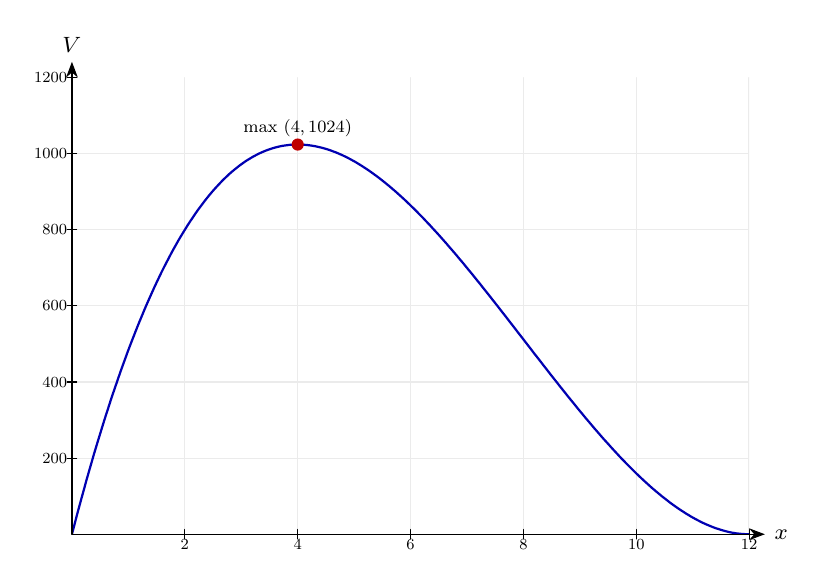
\begin{tikzpicture}[>={Stealth[length=2mm]},font=\footnotesize,line cap=round,line join=round]
\begin{scope}
\clip (0,0) rectangle (8.6,5.8);
\draw[gray!16] (0,0) grid[xstep=1.433,ystep=0.967] (8.6,5.8);
\draw[blue!70!black,thick] (0,0) -- (0.031,0.118) -- (0.061,0.235) -- (0.092,0.35) -- (0.123,0.464) -- (0.154,0.575) -- (0.184,0.686) -- (0.215,0.794) -- (0.246,0.901) -- (0.276,1.006) -- (0.307,1.109) -- (0.338,1.211) -- (0.369,1.312) -- (0.399,1.41) -- (0.43,1.508) -- (0.461,1.603) -- (0.491,1.697) -- (0.522,1.79) -- (0.553,1.88) -- (0.584,1.97) -- (0.614,2.058) -- (0.645,2.144) -- (0.676,2.229) -- (0.706,2.312) -- (0.737,2.394) -- (0.768,2.474) -- (0.799,2.553) -- (0.829,2.63) -- (0.86,2.706) -- (0.891,2.78) -- (0.921,2.853) -- (0.952,2.925) -- (0.983,2.995) -- (1.014,3.064) -- (1.044,3.131) -- (1.075,3.197) -- (1.106,3.262) -- (1.136,3.325) -- (1.167,3.387) -- (1.198,3.447) -- (1.229,3.506) -- (1.259,3.564) -- (1.29,3.621) -- (1.321,3.676) -- (1.351,3.73) -- (1.382,3.782) -- (1.413,3.833) -- (1.444,3.883) -- (1.474,3.932) -- (1.505,3.979) -- (1.536,4.025) -- (1.566,4.07) -- (1.597,4.114) -- (1.628,4.156) -- (1.659,4.197) -- (1.689,4.237) -- (1.72,4.276) -- (1.751,4.314) -- (1.781,4.35) -- (1.812,4.385) -- (1.843,4.419) -- (1.874,4.452) -- (1.904,4.484) -- (1.935,4.515) -- (1.966,4.544) -- (1.996,4.573) -- (2.027,4.6) -- (2.058,4.626) -- (2.089,4.651) -- (2.119,4.675) -- (2.15,4.698) -- (2.181,4.72) -- (2.211,4.741) -- (2.242,4.76) -- (2.273,4.779) -- (2.304,4.797) -- (2.334,4.813) -- (2.365,4.829) -- (2.396,4.844) -- (2.426,4.857) -- (2.457,4.87) -- (2.488,4.882) -- (2.519,4.892) -- (2.549,4.902) -- (2.58,4.911) -- (2.611,4.919) -- (2.641,4.926) -- (2.672,4.932) -- (2.703,4.937) -- (2.734,4.941) -- (2.764,4.945) -- (2.795,4.947) -- (2.826,4.949) -- (2.856,4.949) -- (2.887,4.949) -- (2.918,4.948) -- (2.949,4.946) -- (2.979,4.944) -- (3.01,4.94) -- (3.041,4.936) -- (3.071,4.931) -- (3.102,4.925) -- (3.133,4.918) -- (3.164,4.911) -- (3.194,4.903) -- (3.225,4.894) -- (3.256,4.884) -- (3.286,4.874) -- (3.317,4.862) -- (3.348,4.851) -- (3.379,4.838) -- (3.409,4.825) -- (3.44,4.811) -- (3.471,4.796) -- (3.501,4.781) -- (3.532,4.765) -- (3.563,4.748) -- (3.594,4.731) -- (3.624,4.713) -- (3.655,4.694) -- (3.686,4.675) -- (3.716,4.655) -- (3.747,4.635) -- (3.778,4.614) -- (3.809,4.592) -- (3.839,4.57) -- (3.87,4.548) -- (3.901,4.524) -- (3.931,4.501) -- (3.962,4.476) -- (3.993,4.451) -- (4.024,4.426) -- (4.054,4.4) -- (4.085,4.374) -- (4.116,4.347) -- (4.146,4.32) -- (4.177,4.292) -- (4.208,4.264) -- (4.239,4.235) -- (4.269,4.206) -- (4.3,4.176) -- (4.331,4.146) -- (4.361,4.116) -- (4.392,4.085) -- (4.423,4.053) -- (4.454,4.022) -- (4.484,3.99) -- (4.515,3.957) -- (4.546,3.925) -- (4.576,3.891) -- (4.607,3.858) -- (4.638,3.824) -- (4.669,3.79) -- (4.699,3.756) -- (4.73,3.721) -- (4.761,3.686) -- (4.791,3.65) -- (4.822,3.615) -- (4.853,3.579) -- (4.884,3.543) -- (4.914,3.506) -- (4.945,3.47) -- (4.976,3.433) -- (5.006,3.396) -- (5.037,3.358) -- (5.068,3.321) -- (5.099,3.283) -- (5.129,3.245) -- (5.16,3.207) -- (5.191,3.169) -- (5.221,3.13) -- (5.252,3.092) -- (5.283,3.053) -- (5.314,3.014) -- (5.344,2.975) -- (5.375,2.936) -- (5.406,2.897) -- (5.436,2.858) -- (5.467,2.818) -- (5.498,2.779) -- (5.529,2.739) -- (5.559,2.7) -- (5.59,2.66) -- (5.621,2.62) -- (5.651,2.581) -- (5.682,2.541) -- (5.713,2.501) -- (5.744,2.461) -- (5.774,2.422) -- (5.805,2.382) -- (5.836,2.342) -- (5.866,2.302) -- (5.897,2.263) -- (5.928,2.223) -- (5.959,2.184) -- (5.989,2.144) -- (6.02,2.105) -- (6.051,2.065) -- (6.081,2.026) -- (6.112,1.987) -- (6.143,1.948) -- (6.174,1.909) -- (6.204,1.87) -- (6.235,1.832) -- (6.266,1.793) -- (6.296,1.755) -- (6.327,1.717) -- (6.358,1.679) -- (6.389,1.641) -- (6.419,1.603) -- (6.45,1.566) -- (6.481,1.529) -- (6.511,1.492) -- (6.542,1.455) -- (6.573,1.419) -- (6.604,1.382) -- (6.634,1.346) -- (6.665,1.311) -- (6.696,1.275) -- (6.726,1.24) -- (6.757,1.205) -- (6.788,1.171) -- (6.819,1.137) -- (6.849,1.103) -- (6.88,1.069) -- (6.911,1.036) -- (6.941,1.003) -- (6.972,0.97) -- (7.003,0.938) -- (7.034,0.906) -- (7.064,0.875) -- (7.095,0.844) -- (7.126,0.813) -- (7.156,0.783) -- (7.187,0.754) -- (7.218,0.724) -- (7.249,0.695) -- (7.279,0.667) -- (7.31,0.639) -- (7.341,0.611) -- (7.371,0.584) -- (7.402,0.558) -- (7.433,0.532) -- (7.464,0.506) -- (7.494,0.481) -- (7.525,0.457) -- (7.556,0.433) -- (7.586,0.409) -- (7.617,0.386) -- (7.648,0.364) -- (7.679,0.342) -- (7.709,0.321) -- (7.74,0.301) -- (7.771,0.281) -- (7.801,0.261) -- (7.832,0.243) -- (7.863,0.224) -- (7.894,0.207) -- (7.924,0.19) -- (7.955,0.174) -- (7.986,0.158) -- (8.016,0.143) -- (8.047,0.129) -- (8.078,0.116) -- (8.109,0.103) -- (8.139,0.091) -- (8.17,0.079) -- (8.201,0.069) -- (8.231,0.059) -- (8.262,0.05) -- (8.293,0.041) -- (8.324,0.033) -- (8.354,0.026) -- (8.385,0.02) -- (8.416,0.015) -- (8.446,0.01) -- (8.477,0.007) -- (8.508,0.004) -- (8.539,0.002) -- (8.569,0) -- (8.6,0);
\end{scope}
\draw[->] (0,0) -- (8.8,0) node[right]{$x$};
\draw[->] (0,0) -- (0,6) node[above]{$V$};
\draw (1.433,-0.06) -- (1.433,0.06) node[below=1pt,scale=0.7]{$2$};
\draw (2.867,-0.06) -- (2.867,0.06) node[below=1pt,scale=0.7]{$4$};
\draw (4.3,-0.06) -- (4.3,0.06) node[below=1pt,scale=0.7]{$6$};
\draw (5.733,-0.06) -- (5.733,0.06) node[below=1pt,scale=0.7]{$8$};
\draw (7.167,-0.06) -- (7.167,0.06) node[below=1pt,scale=0.7]{$10$};
\draw (8.6,-0.06) -- (8.6,0.06) node[below=1pt,scale=0.7]{$12$};
\draw (-0.06,0.967) -- (0.06,0.967) node[left=1pt,scale=0.7]{$200$};
\draw (-0.06,1.933) -- (0.06,1.933) node[left=1pt,scale=0.7]{$400$};
\draw (-0.06,2.9) -- (0.06,2.9) node[left=1pt,scale=0.7]{$600$};
\draw (-0.06,3.867) -- (0.06,3.867) node[left=1pt,scale=0.7]{$800$};
\draw (-0.06,4.833) -- (0.06,4.833) node[left=1pt,scale=0.7]{$1000$};
\draw (-0.06,5.8) -- (0.06,5.8) node[left=1pt,scale=0.7]{$1200$};
\fill[red!75!black] (2.867,4.949) circle (2.2pt);
\node[above,scale=0.78] at (2.867,4.949) {max $(4,1024)$};
\end{tikzpicture}
}
\end{center}
\small The model plotted against its variable, with the key point(s) marked.\normalsize

\medskip\hrule

\section*{Real-Life Problems 18\quad\small\texttt{(d5-018)}}
\addcontentsline{toc}{section}{Real-Life Problems 18 (d5-018)}
\textit{Difficulty: Foundation \quad\textbar\quad Marks: 6}

\question{A rectangular sheet of cardboard measures \( 20 \) cm by \( 12 \) cm. Equal squares of side \( x \) cm are cut from each corner and the sides folded up to form an open box. (a) Show that the volume is \( V = 4x^3 - 64x^2 + 240x \). (b) Find the value of \( x \) that maximises the volume.}

\textbf{Worked solution.}

\textit{Step 1: (a) After cutting, the box has dimensions \( (20-2x) \times (12-2x) \times x \).}
\[\begin{gathered}
V = x(20-2x)(12-2x)
\end{gathered}\]
Length, width and height of the open box.

\textit{Step 2: Expand.}
\[\begin{gathered}
V = x(240 - 40x - 24x + 4x^2) = x(240 - 64x + 4x^2) = 240x - 64x^2 + 4x^3
\end{gathered}\]
Multiply out and simplify.

\textit{Step 3: (b) Differentiate.}
\[\begin{gathered}
\frac{\mathrm{d}V}{\mathrm{d}x} = 240 - 128x + 12x^2
\end{gathered}\]
Power rule.

\textit{Step 4: Set to zero.}
\[\begin{gathered}
12x^2 - 128x + 240 = 0 \implies 3x^2 - 32x + 60 = 0
\end{gathered}\]
Divide by 4 to simplify. This quadratic does not factorise over the integers (testing \( x = 2 \): \( 12 - 64 + 60 = 8 \neq 0 \)), so the quadratic formula is needed.

\textit{Step 5: Use the quadratic formula.}
\[\begin{gathered}
x = \frac{32 \pm \sqrt{1024 - 720}}{6} = \frac{32 \pm \sqrt{304}}{6} \approx \frac{32 \pm 17.44}{6}
\end{gathered}\]
\( a = 12, b = -128, c = 240 \).

\textit{Step 6: Select valid solution.}
\[\begin{gathered}
x \approx \frac{32 - 17.44}{6} \approx 2.43 \text{ cm (to 3 s.f.)}; \quad x \approx 8.24 \text{ rejected (} > 6\text{)}
\end{gathered}\]
The maximum allowed \( x \) is half the shortest side: \( \tfrac{12}{2} = 6 \) cm. So \( x \approx 8.24 \) is rejected.

\begin{answerbox}
\textbf{Final answer:}\quad (a) Shown: \(\displaystyle  V = 4x^3 - 64x^2 + 240x \) \\[3pt]  (b) \(\displaystyle  x \approx 2.43 \) cm
\end{answerbox}
\textbf{Diagram.}

\begin{center}
\resizebox{\ifdim\width>\linewidth \linewidth\else \width\fi}{!}{%
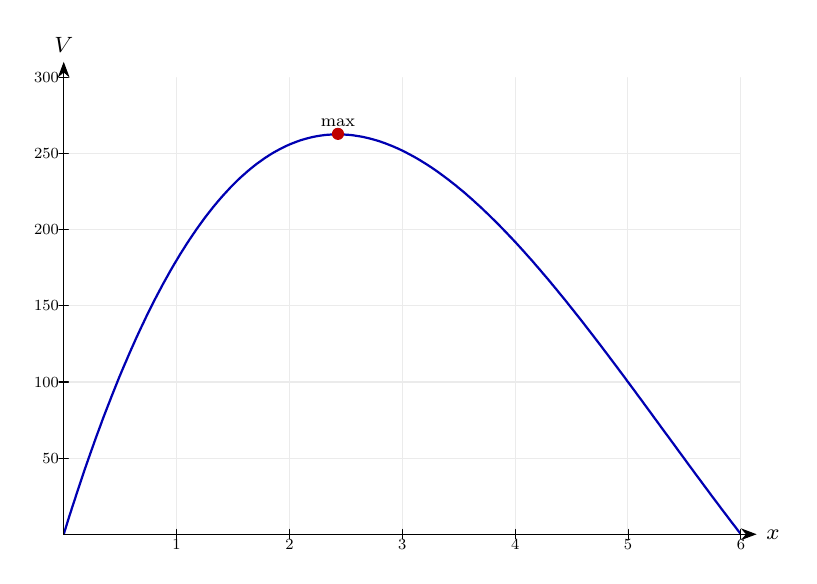
\begin{tikzpicture}[>={Stealth[length=2mm]},font=\footnotesize,line cap=round,line join=round]
\begin{scope}
\clip (0,0) rectangle (8.6,5.8);
\draw[gray!16] (0,0) grid[xstep=1.433,ystep=0.967] (8.6,5.8);
\draw[blue!70!black,thick] (0,0) -- (0.031,0.099) -- (0.061,0.197) -- (0.092,0.293) -- (0.123,0.389) -- (0.154,0.483) -- (0.184,0.576) -- (0.215,0.668) -- (0.246,0.759) -- (0.276,0.849) -- (0.307,0.938) -- (0.338,1.026) -- (0.369,1.113) -- (0.399,1.198) -- (0.43,1.283) -- (0.461,1.366) -- (0.491,1.449) -- (0.522,1.53) -- (0.553,1.61) -- (0.584,1.689) -- (0.614,1.767) -- (0.645,1.844) -- (0.676,1.921) -- (0.706,1.996) -- (0.737,2.07) -- (0.768,2.143) -- (0.799,2.214) -- (0.829,2.285) -- (0.86,2.355) -- (0.891,2.424) -- (0.921,2.492) -- (0.952,2.559) -- (0.983,2.625) -- (1.014,2.69) -- (1.044,2.754) -- (1.075,2.817) -- (1.106,2.879) -- (1.136,2.94) -- (1.167,3) -- (1.198,3.059) -- (1.229,3.117) -- (1.259,3.174) -- (1.29,3.23) -- (1.321,3.285) -- (1.351,3.34) -- (1.382,3.393) -- (1.413,3.446) -- (1.444,3.497) -- (1.474,3.548) -- (1.505,3.597) -- (1.536,3.646) -- (1.566,3.694) -- (1.597,3.741) -- (1.628,3.787) -- (1.659,3.832) -- (1.689,3.876) -- (1.72,3.92) -- (1.751,3.962) -- (1.781,4.004) -- (1.812,4.045) -- (1.843,4.085) -- (1.874,4.124) -- (1.904,4.162) -- (1.935,4.199) -- (1.966,4.236) -- (1.996,4.271) -- (2.027,4.306) -- (2.058,4.34) -- (2.089,4.373) -- (2.119,4.406) -- (2.15,4.437) -- (2.181,4.468) -- (2.211,4.498) -- (2.242,4.527) -- (2.273,4.555) -- (2.304,4.582) -- (2.334,4.609) -- (2.365,4.635) -- (2.396,4.66) -- (2.426,4.684) -- (2.457,4.708) -- (2.488,4.73) -- (2.519,4.752) -- (2.549,4.774) -- (2.58,4.794) -- (2.611,4.814) -- (2.641,4.833) -- (2.672,4.851) -- (2.703,4.868) -- (2.734,4.885) -- (2.764,4.901) -- (2.795,4.916) -- (2.826,4.931) -- (2.856,4.945) -- (2.887,4.958) -- (2.918,4.97) -- (2.949,4.982) -- (2.979,4.993) -- (3.01,5.004) -- (3.041,5.013) -- (3.071,5.022) -- (3.102,5.03) -- (3.133,5.038) -- (3.164,5.045) -- (3.194,5.051) -- (3.225,5.057) -- (3.256,5.062) -- (3.286,5.066) -- (3.317,5.07) -- (3.348,5.073) -- (3.379,5.075) -- (3.409,5.077) -- (3.44,5.078) -- (3.471,5.078) -- (3.501,5.078) -- (3.532,5.078) -- (3.563,5.076) -- (3.594,5.074) -- (3.624,5.072) -- (3.655,5.069) -- (3.686,5.065) -- (3.716,5.06) -- (3.747,5.055) -- (3.778,5.05) -- (3.809,5.044) -- (3.839,5.037) -- (3.87,5.03) -- (3.901,5.022) -- (3.931,5.014) -- (3.962,5.005) -- (3.993,4.996) -- (4.024,4.986) -- (4.054,4.975) -- (4.085,4.964) -- (4.116,4.952) -- (4.146,4.94) -- (4.177,4.928) -- (4.208,4.914) -- (4.239,4.901) -- (4.269,4.887) -- (4.3,4.872) -- (4.331,4.857) -- (4.361,4.841) -- (4.392,4.825) -- (4.423,4.808) -- (4.454,4.791) -- (4.484,4.774) -- (4.515,4.756) -- (4.546,4.737) -- (4.576,4.718) -- (4.607,4.699) -- (4.638,4.679) -- (4.669,4.659) -- (4.699,4.638) -- (4.73,4.617) -- (4.761,4.595) -- (4.791,4.573) -- (4.822,4.55) -- (4.853,4.527) -- (4.884,4.504) -- (4.914,4.48) -- (4.945,4.456) -- (4.976,4.432) -- (5.006,4.407) -- (5.037,4.381) -- (5.068,4.356) -- (5.099,4.33) -- (5.129,4.303) -- (5.16,4.276) -- (5.191,4.249) -- (5.221,4.221) -- (5.252,4.193) -- (5.283,4.165) -- (5.314,4.136) -- (5.344,4.107) -- (5.375,4.078) -- (5.406,4.048) -- (5.436,4.018) -- (5.467,3.988) -- (5.498,3.957) -- (5.529,3.926) -- (5.559,3.895) -- (5.59,3.863) -- (5.621,3.832) -- (5.651,3.799) -- (5.682,3.767) -- (5.713,3.734) -- (5.744,3.701) -- (5.774,3.668) -- (5.805,3.634) -- (5.836,3.6) -- (5.866,3.566) -- (5.897,3.531) -- (5.928,3.497) -- (5.959,3.462) -- (5.989,3.426) -- (6.02,3.391) -- (6.051,3.355) -- (6.081,3.319) -- (6.112,3.283) -- (6.143,3.247) -- (6.174,3.21) -- (6.204,3.173) -- (6.235,3.136) -- (6.266,3.099) -- (6.296,3.061) -- (6.327,3.024) -- (6.358,2.986) -- (6.389,2.948) -- (6.419,2.909) -- (6.45,2.871) -- (6.481,2.832) -- (6.511,2.794) -- (6.542,2.755) -- (6.573,2.716) -- (6.604,2.676) -- (6.634,2.637) -- (6.665,2.597) -- (6.696,2.557) -- (6.726,2.518) -- (6.757,2.478) -- (6.788,2.437) -- (6.819,2.397) -- (6.849,2.357) -- (6.88,2.316) -- (6.911,2.276) -- (6.941,2.235) -- (6.972,2.194) -- (7.003,2.153) -- (7.034,2.112) -- (7.064,2.071) -- (7.095,2.03) -- (7.126,1.989) -- (7.156,1.947) -- (7.187,1.906) -- (7.218,1.864) -- (7.249,1.823) -- (7.279,1.781) -- (7.31,1.739) -- (7.341,1.698) -- (7.371,1.656) -- (7.402,1.614) -- (7.433,1.572) -- (7.464,1.53) -- (7.494,1.488) -- (7.525,1.446) -- (7.556,1.404) -- (7.586,1.362) -- (7.617,1.32) -- (7.648,1.278) -- (7.679,1.237) -- (7.709,1.195) -- (7.74,1.153) -- (7.771,1.111) -- (7.801,1.069) -- (7.832,1.027) -- (7.863,0.985) -- (7.894,0.943) -- (7.924,0.901) -- (7.955,0.859) -- (7.986,0.818) -- (8.016,0.776) -- (8.047,0.734) -- (8.078,0.693) -- (8.109,0.651) -- (8.139,0.61) -- (8.17,0.569) -- (8.201,0.527) -- (8.231,0.486) -- (8.262,0.445) -- (8.293,0.404) -- (8.324,0.363) -- (8.354,0.322) -- (8.385,0.282) -- (8.416,0.241) -- (8.446,0.201) -- (8.477,0.16) -- (8.508,0.12) -- (8.539,0.08) -- (8.569,0.04) -- (8.6,0);
\end{scope}
\draw[->] (0,0) -- (8.8,0) node[right]{$x$};
\draw[->] (0,0) -- (0,6) node[above]{$V$};
\draw (1.433,-0.06) -- (1.433,0.06) node[below=1pt,scale=0.7]{$1$};
\draw (2.867,-0.06) -- (2.867,0.06) node[below=1pt,scale=0.7]{$2$};
\draw (4.3,-0.06) -- (4.3,0.06) node[below=1pt,scale=0.7]{$3$};
\draw (5.733,-0.06) -- (5.733,0.06) node[below=1pt,scale=0.7]{$4$};
\draw (7.167,-0.06) -- (7.167,0.06) node[below=1pt,scale=0.7]{$5$};
\draw (8.6,-0.06) -- (8.6,0.06) node[below=1pt,scale=0.7]{$6$};
\draw (-0.06,0.967) -- (0.06,0.967) node[left=1pt,scale=0.7]{$50$};
\draw (-0.06,1.933) -- (0.06,1.933) node[left=1pt,scale=0.7]{$100$};
\draw (-0.06,2.9) -- (0.06,2.9) node[left=1pt,scale=0.7]{$150$};
\draw (-0.06,3.867) -- (0.06,3.867) node[left=1pt,scale=0.7]{$200$};
\draw (-0.06,4.833) -- (0.06,4.833) node[left=1pt,scale=0.7]{$250$};
\draw (-0.06,5.8) -- (0.06,5.8) node[left=1pt,scale=0.7]{$300$};
\fill[red!75!black] (3.483,5.085) circle (2.2pt);
\node[above,scale=0.78] at (3.483,5.085) {max};
\end{tikzpicture}
}
\end{center}
\small The model plotted against its variable, with the key point(s) marked.\normalsize

\medskip\hrule

\section*{Real-Life Problems 19\quad\small\texttt{(d5-019)}}
\addcontentsline{toc}{section}{Real-Life Problems 19 (d5-019)}
\textit{Difficulty: Foundation \quad\textbar\quad Marks: 7}

\question{A cylindrical storage tank (open at the top) has radius \( r \) m and height \( h \) m. The volume must be \( 16\pi \) m\(^3\). (a) Express \( h \) in terms of \( r \). (b) Show that the surface area (base + curved side) is \( A = \pi r^2 + \dfrac{32\pi}{r} \). (c) Find the value of \( r \) that minimises the surface area.}

\textbf{Worked solution.}

\textit{Step 1: (a) Use the volume formula.}
\[\begin{gathered}
\pi r^2 h = 16\pi \implies h = \frac{16}{r^2}
\end{gathered}\]
Rearrange to make \( h \) the subject.

\textit{Step 2: (b) Surface area = base + curved side.}
\[\begin{gathered}
A = \pi r^2 + 2\pi r h = \pi r^2 + 2\pi r \cdot \frac{16}{r^2} = \pi r^2 + \frac{32\pi}{r}
\end{gathered}\]
Substitute \( h = \dfrac{16}{r^2} \).

\textit{Step 3: (c) Differentiate.}
\[\begin{gathered}
\frac{\mathrm{d}A}{\mathrm{d}r} = 2\pi r - \frac{32\pi}{r^2}
\end{gathered}\]
\( \dfrac{\mathrm{d}}{\mathrm{d}r}\left(\dfrac{32\pi}{r}\right) = -\dfrac{32\pi}{r^2} \).

\textit{Step 4: Set to zero.}
\[\begin{gathered}
2\pi r = \frac{32\pi}{r^2} \implies 2r^3 = 32 \implies r^3 = 16 \implies r = 2\sqrt[3]{2} \approx 2.52 \text{ m}
\end{gathered}\]
Multiply by \( r^2 \) and solve for \( r \).

\textit{Step 5: Confirm minimum.}
\[\begin{gathered}
\frac{\mathrm{d}^2A}{\mathrm{d}r^2} = 2\pi + \frac{64\pi}{r^3} > 0 \Rightarrow \text{minimum}
\end{gathered}\]
Both terms are positive, so the second derivative is always positive.

\begin{answerbox}
\textbf{Final answer:}\quad (a) \(\displaystyle  h = \dfrac{16}{r^2} \) \\[3pt]  (b) Shown. \\[3pt]  (c) \(\displaystyle  r = 2\sqrt[3]{2} \approx 2.52 \) m
\end{answerbox}
\textbf{Diagram.}

\begin{center}
\resizebox{\ifdim\width>\linewidth \linewidth\else \width\fi}{!}{%
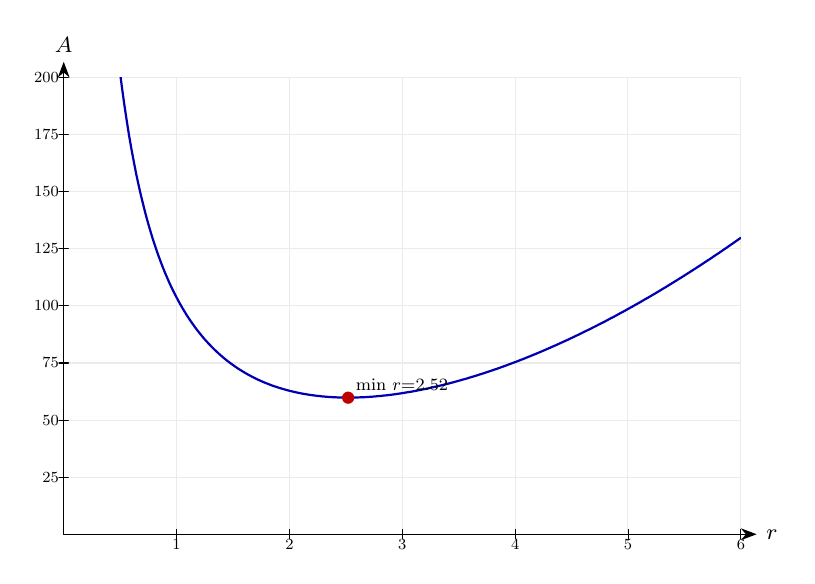
\begin{tikzpicture}[>={Stealth[length=2mm]},font=\footnotesize,line cap=round,line join=round]
\begin{scope}
\clip (0,0) rectangle (8.6,5.8);
\draw[gray!16] (0,0) grid[xstep=1.433,ystep=0.725] (8.6,5.8);
\draw[blue!70!black,thick] (0.031,11.6) -- (0.061,11.6) -- (0.092,11.6) -- (0.123,11.6) -- (0.154,11.6) -- (0.184,11.6) -- (0.215,11.6) -- (0.246,11.6) -- (0.276,11.6) -- (0.307,11.6) -- (0.338,11.6) -- (0.369,11.344) -- (0.399,10.473) -- (0.43,9.726) -- (0.461,9.08) -- (0.491,8.514) -- (0.522,8.015) -- (0.553,7.572) -- (0.584,7.176) -- (0.614,6.819) -- (0.645,6.497) -- (0.676,6.204) -- (0.706,5.937) -- (0.737,5.693) -- (0.768,5.468) -- (0.799,5.261) -- (0.829,5.069) -- (0.86,4.892) -- (0.891,4.727) -- (0.921,4.573) -- (0.952,4.429) -- (0.983,4.294) -- (1.014,4.168) -- (1.044,4.05) -- (1.075,3.938) -- (1.106,3.833) -- (1.136,3.734) -- (1.167,3.641) -- (1.198,3.552) -- (1.229,3.468) -- (1.259,3.389) -- (1.29,3.313) -- (1.321,3.241) -- (1.351,3.173) -- (1.382,3.108) -- (1.413,3.046) -- (1.444,2.987) -- (1.474,2.931) -- (1.505,2.877) -- (1.536,2.826) -- (1.566,2.776) -- (1.597,2.73) -- (1.628,2.685) -- (1.659,2.641) -- (1.689,2.6) -- (1.72,2.561) -- (1.751,2.523) -- (1.781,2.486) -- (1.812,2.452) -- (1.843,2.418) -- (1.874,2.386) -- (1.904,2.355) -- (1.935,2.326) -- (1.966,2.297) -- (1.996,2.27) -- (2.027,2.244) -- (2.058,2.218) -- (2.089,2.194) -- (2.119,2.171) -- (2.15,2.149) -- (2.181,2.127) -- (2.211,2.106) -- (2.242,2.087) -- (2.273,2.068) -- (2.304,2.049) -- (2.334,2.032) -- (2.365,2.015) -- (2.396,1.999) -- (2.426,1.983) -- (2.457,1.968) -- (2.488,1.954) -- (2.519,1.94) -- (2.549,1.927) -- (2.58,1.915) -- (2.611,1.903) -- (2.641,1.891) -- (2.672,1.88) -- (2.703,1.87) -- (2.734,1.86) -- (2.764,1.851) -- (2.795,1.842) -- (2.826,1.833) -- (2.856,1.825) -- (2.887,1.817) -- (2.918,1.81) -- (2.949,1.803) -- (2.979,1.796) -- (3.01,1.79) -- (3.041,1.784) -- (3.071,1.779) -- (3.102,1.774) -- (3.133,1.769) -- (3.164,1.765) -- (3.194,1.761) -- (3.225,1.757) -- (3.256,1.754) -- (3.286,1.75) -- (3.317,1.748) -- (3.348,1.745) -- (3.379,1.743) -- (3.409,1.741) -- (3.44,1.74) -- (3.471,1.738) -- (3.501,1.737) -- (3.532,1.736) -- (3.563,1.736) -- (3.594,1.736) -- (3.624,1.735) -- (3.655,1.736) -- (3.686,1.736) -- (3.716,1.737) -- (3.747,1.738) -- (3.778,1.739) -- (3.809,1.74) -- (3.839,1.742) -- (3.87,1.744) -- (3.901,1.746) -- (3.931,1.748) -- (3.962,1.751) -- (3.993,1.754) -- (4.024,1.756) -- (4.054,1.76) -- (4.085,1.763) -- (4.116,1.766) -- (4.146,1.77) -- (4.177,1.774) -- (4.208,1.778) -- (4.239,1.783) -- (4.269,1.787) -- (4.3,1.792) -- (4.331,1.797) -- (4.361,1.802) -- (4.392,1.807) -- (4.423,1.812) -- (4.454,1.818) -- (4.484,1.824) -- (4.515,1.83) -- (4.546,1.836) -- (4.576,1.842) -- (4.607,1.848) -- (4.638,1.855) -- (4.669,1.862) -- (4.699,1.869) -- (4.73,1.876) -- (4.761,1.883) -- (4.791,1.89) -- (4.822,1.898) -- (4.853,1.905) -- (4.884,1.913) -- (4.914,1.921) -- (4.945,1.929) -- (4.976,1.938) -- (5.006,1.946) -- (5.037,1.955) -- (5.068,1.964) -- (5.099,1.972) -- (5.129,1.981) -- (5.16,1.991) -- (5.191,2) -- (5.221,2.009) -- (5.252,2.019) -- (5.283,2.029) -- (5.314,2.038) -- (5.344,2.048) -- (5.375,2.059) -- (5.406,2.069) -- (5.436,2.079) -- (5.467,2.09) -- (5.498,2.1) -- (5.529,2.111) -- (5.559,2.122) -- (5.59,2.133) -- (5.621,2.144) -- (5.651,2.156) -- (5.682,2.167) -- (5.713,2.179) -- (5.744,2.19) -- (5.774,2.202) -- (5.805,2.214) -- (5.836,2.226) -- (5.866,2.238) -- (5.897,2.251) -- (5.928,2.263) -- (5.959,2.276) -- (5.989,2.288) -- (6.02,2.301) -- (6.051,2.314) -- (6.081,2.327) -- (6.112,2.34) -- (6.143,2.354) -- (6.174,2.367) -- (6.204,2.381) -- (6.235,2.394) -- (6.266,2.408) -- (6.296,2.422) -- (6.327,2.436) -- (6.358,2.45) -- (6.389,2.464) -- (6.419,2.478) -- (6.45,2.493) -- (6.481,2.507) -- (6.511,2.522) -- (6.542,2.537) -- (6.573,2.552) -- (6.604,2.567) -- (6.634,2.582) -- (6.665,2.597) -- (6.696,2.612) -- (6.726,2.628) -- (6.757,2.643) -- (6.788,2.659) -- (6.819,2.675) -- (6.849,2.69) -- (6.88,2.706) -- (6.911,2.723) -- (6.941,2.739) -- (6.972,2.755) -- (7.003,2.771) -- (7.034,2.788) -- (7.064,2.805) -- (7.095,2.821) -- (7.126,2.838) -- (7.156,2.855) -- (7.187,2.872) -- (7.218,2.889) -- (7.249,2.907) -- (7.279,2.924) -- (7.31,2.941) -- (7.341,2.959) -- (7.371,2.977) -- (7.402,2.994) -- (7.433,3.012) -- (7.464,3.03) -- (7.494,3.048) -- (7.525,3.066) -- (7.556,3.085) -- (7.586,3.103) -- (7.617,3.122) -- (7.648,3.14) -- (7.679,3.159) -- (7.709,3.178) -- (7.74,3.197) -- (7.771,3.216) -- (7.801,3.235) -- (7.832,3.254) -- (7.863,3.273) -- (7.894,3.293) -- (7.924,3.312) -- (7.955,3.332) -- (7.986,3.351) -- (8.016,3.371) -- (8.047,3.391) -- (8.078,3.411) -- (8.109,3.431) -- (8.139,3.451) -- (8.17,3.472) -- (8.201,3.492) -- (8.231,3.512) -- (8.262,3.533) -- (8.293,3.554) -- (8.324,3.574) -- (8.354,3.595) -- (8.385,3.616) -- (8.416,3.637) -- (8.446,3.658) -- (8.477,3.68) -- (8.508,3.701) -- (8.539,3.723) -- (8.569,3.744) -- (8.6,3.766);
\end{scope}
\draw[->] (0,0) -- (8.8,0) node[right]{$r$};
\draw[->] (0,0) -- (0,6) node[above]{$A$};
\draw (1.433,-0.06) -- (1.433,0.06) node[below=1pt,scale=0.7]{$1$};
\draw (2.867,-0.06) -- (2.867,0.06) node[below=1pt,scale=0.7]{$2$};
\draw (4.3,-0.06) -- (4.3,0.06) node[below=1pt,scale=0.7]{$3$};
\draw (5.733,-0.06) -- (5.733,0.06) node[below=1pt,scale=0.7]{$4$};
\draw (7.167,-0.06) -- (7.167,0.06) node[below=1pt,scale=0.7]{$5$};
\draw (8.6,-0.06) -- (8.6,0.06) node[below=1pt,scale=0.7]{$6$};
\draw (-0.06,0.725) -- (0.06,0.725) node[left=1pt,scale=0.7]{$25$};
\draw (-0.06,1.45) -- (0.06,1.45) node[left=1pt,scale=0.7]{$50$};
\draw (-0.06,2.175) -- (0.06,2.175) node[left=1pt,scale=0.7]{$75$};
\draw (-0.06,2.9) -- (0.06,2.9) node[left=1pt,scale=0.7]{$100$};
\draw (-0.06,3.625) -- (0.06,3.625) node[left=1pt,scale=0.7]{$125$};
\draw (-0.06,4.35) -- (0.06,4.35) node[left=1pt,scale=0.7]{$150$};
\draw (-0.06,5.075) -- (0.06,5.075) node[left=1pt,scale=0.7]{$175$};
\draw (-0.06,5.8) -- (0.06,5.8) node[left=1pt,scale=0.7]{$200$};
\fill[red!75!black] (3.612,1.734) circle (2.2pt);
\node[above right,scale=0.78] at (3.612,1.734) {min $r{=}2.52$};
\end{tikzpicture}
}
\end{center}
\small The model plotted against its variable, with the key point(s) marked.\normalsize

\medskip\hrule

\section*{Real-Life Problems 20\quad\small\texttt{(d5-020)}}
\addcontentsline{toc}{section}{Real-Life Problems 20 (d5-020)}
\textit{Difficulty: Foundation \quad\textbar\quad Marks: 6}

\question{A particle's displacement is \( s = t^4 - 8t^2 \) metres after \( t \) seconds for \( t \geq 0 \). (a) Find the velocity and acceleration functions. (b) Find the values of \( t \) when the particle is at rest. (c) Find the acceleration at each of those times.}

\textbf{Worked solution.}

\textit{Step 1: (a) Velocity.}
\[\begin{gathered}
v = \frac{\mathrm{d}s}{\mathrm{d}t} = 4t^3 - 16t
\end{gathered}\]
Differentiate \( s \).

\textit{Step 2: Acceleration.}
\[\begin{gathered}
a = \frac{\mathrm{d}v}{\mathrm{d}t} = 12t^2 - 16
\end{gathered}\]
Differentiate \( v \).

\textit{Step 3: (b) Set \( v = 0 \).}
\[\begin{gathered}
4t^3 - 16t = 0 \implies 4t(t^2 - 4) = 0 \implies t = 0, \; t = 2 \; (t = -2 \text{ rejected})
\end{gathered}\]
For \( t \geq 0 \), only \( t = 0 \) and \( t = 2 \) are valid.

\textit{Step 4: (c) Acceleration at rest times.}
\[\begin{gathered}
a(0) = -16 \text{ ms}^{-2}; \quad a(2) = 12(4) - 16 = 32 \text{ ms}^{-2}
\end{gathered}\]
Substitute \( t = 0 \) and \( t = 2 \) into \( a = 12t^2 - 16 \).

\begin{answerbox}
\textbf{Final answer:}\quad (a) \(\displaystyle  v = 4t^3 - 16t \), \(\displaystyle  a = 12t^2 - 16 \) \\[3pt]  (b) \(\displaystyle  t = 0 \) and \(\displaystyle  t = 2 \) s \\[3pt]  (c) \(\displaystyle  -16 \text{ ms}^{-2} \) and \(\displaystyle  32 \text{ ms}^{-2} \)
\end{answerbox}
\textbf{Diagram.}

\begin{center}
\resizebox{\ifdim\width>\linewidth \linewidth\else \width\fi}{!}{%
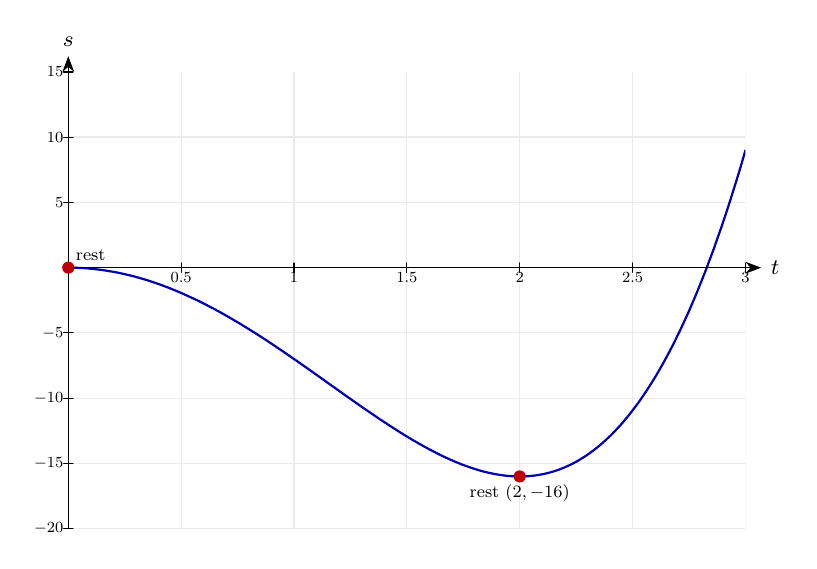
\begin{tikzpicture}[>={Stealth[length=2mm]},font=\footnotesize,line cap=round,line join=round]
\begin{scope}
\clip (0,0) rectangle (8.6,5.8);
\draw[gray!16] (0,0) grid[xstep=1.433,ystep=0.829] (8.6,5.8);
\draw[blue!70!black,thick] (0,3.314) -- (0.031,3.314) -- (0.061,3.314) -- (0.092,3.313) -- (0.123,3.312) -- (0.154,3.31) -- (0.184,3.309) -- (0.215,3.307) -- (0.246,3.305) -- (0.276,3.302) -- (0.307,3.299) -- (0.338,3.296) -- (0.369,3.292) -- (0.399,3.289) -- (0.43,3.285) -- (0.461,3.28) -- (0.491,3.275) -- (0.522,3.27) -- (0.553,3.265) -- (0.584,3.26) -- (0.614,3.254) -- (0.645,3.248) -- (0.676,3.241) -- (0.706,3.234) -- (0.737,3.227) -- (0.768,3.22) -- (0.799,3.212) -- (0.829,3.205) -- (0.86,3.196) -- (0.891,3.188) -- (0.921,3.179) -- (0.952,3.17) -- (0.983,3.161) -- (1.014,3.151) -- (1.044,3.141) -- (1.075,3.131) -- (1.106,3.121) -- (1.136,3.11) -- (1.167,3.099) -- (1.198,3.088) -- (1.229,3.076) -- (1.259,3.065) -- (1.29,3.053) -- (1.321,3.04) -- (1.351,3.028) -- (1.382,3.015) -- (1.413,3.002) -- (1.444,2.989) -- (1.474,2.975) -- (1.505,2.961) -- (1.536,2.947) -- (1.566,2.933) -- (1.597,2.919) -- (1.628,2.904) -- (1.659,2.889) -- (1.689,2.874) -- (1.72,2.859) -- (1.751,2.843) -- (1.781,2.827) -- (1.812,2.811) -- (1.843,2.795) -- (1.874,2.778) -- (1.904,2.762) -- (1.935,2.745) -- (1.966,2.728) -- (1.996,2.71) -- (2.027,2.693) -- (2.058,2.675) -- (2.089,2.657) -- (2.119,2.639) -- (2.15,2.621) -- (2.181,2.603) -- (2.211,2.584) -- (2.242,2.565) -- (2.273,2.546) -- (2.304,2.527) -- (2.334,2.508) -- (2.365,2.489) -- (2.396,2.469) -- (2.426,2.45) -- (2.457,2.43) -- (2.488,2.41) -- (2.519,2.39) -- (2.549,2.37) -- (2.58,2.349) -- (2.611,2.329) -- (2.641,2.308) -- (2.672,2.287) -- (2.703,2.267) -- (2.734,2.246) -- (2.764,2.225) -- (2.795,2.204) -- (2.826,2.183) -- (2.856,2.161) -- (2.887,2.14) -- (2.918,2.119) -- (2.949,2.097) -- (2.979,2.076) -- (3.01,2.054) -- (3.041,2.032) -- (3.071,2.011) -- (3.102,1.989) -- (3.133,1.967) -- (3.164,1.946) -- (3.194,1.924) -- (3.225,1.902) -- (3.256,1.88) -- (3.286,1.858) -- (3.317,1.836) -- (3.348,1.814) -- (3.379,1.793) -- (3.409,1.771) -- (3.44,1.749) -- (3.471,1.727) -- (3.501,1.705) -- (3.532,1.684) -- (3.563,1.662) -- (3.594,1.64) -- (3.624,1.619) -- (3.655,1.597) -- (3.686,1.576) -- (3.716,1.554) -- (3.747,1.533) -- (3.778,1.512) -- (3.809,1.491) -- (3.839,1.47) -- (3.87,1.449) -- (3.901,1.428) -- (3.931,1.407) -- (3.962,1.386) -- (3.993,1.366) -- (4.024,1.346) -- (4.054,1.326) -- (4.085,1.306) -- (4.116,1.286) -- (4.146,1.266) -- (4.177,1.247) -- (4.208,1.227) -- (4.239,1.208) -- (4.269,1.189) -- (4.3,1.17) -- (4.331,1.152) -- (4.361,1.133) -- (4.392,1.115) -- (4.423,1.098) -- (4.454,1.08) -- (4.484,1.063) -- (4.515,1.045) -- (4.546,1.029) -- (4.576,1.012) -- (4.607,0.996) -- (4.638,0.98) -- (4.669,0.964) -- (4.699,0.948) -- (4.73,0.933) -- (4.761,0.918) -- (4.791,0.904) -- (4.822,0.89) -- (4.853,0.876) -- (4.884,0.863) -- (4.914,0.849) -- (4.945,0.837) -- (4.976,0.824) -- (5.006,0.812) -- (5.037,0.801) -- (5.068,0.79) -- (5.099,0.779) -- (5.129,0.769) -- (5.16,0.759) -- (5.191,0.749) -- (5.221,0.74) -- (5.252,0.731) -- (5.283,0.723) -- (5.314,0.716) -- (5.344,0.708) -- (5.375,0.702) -- (5.406,0.696) -- (5.436,0.69) -- (5.467,0.685) -- (5.498,0.68) -- (5.529,0.676) -- (5.559,0.672) -- (5.59,0.669) -- (5.621,0.667) -- (5.651,0.665) -- (5.682,0.664) -- (5.713,0.663) -- (5.744,0.663) -- (5.774,0.663) -- (5.805,0.665) -- (5.836,0.666) -- (5.866,0.669) -- (5.897,0.672) -- (5.928,0.675) -- (5.959,0.68) -- (5.989,0.685) -- (6.02,0.691) -- (6.051,0.697) -- (6.081,0.704) -- (6.112,0.712) -- (6.143,0.721) -- (6.174,0.73) -- (6.204,0.74) -- (6.235,0.751) -- (6.266,0.763) -- (6.296,0.775) -- (6.327,0.789) -- (6.358,0.803) -- (6.389,0.818) -- (6.419,0.833) -- (6.45,0.85) -- (6.481,0.867) -- (6.511,0.886) -- (6.542,0.905) -- (6.573,0.925) -- (6.604,0.946) -- (6.634,0.968) -- (6.665,0.99) -- (6.696,1.014) -- (6.726,1.039) -- (6.757,1.064) -- (6.788,1.091) -- (6.819,1.118) -- (6.849,1.147) -- (6.88,1.176) -- (6.911,1.207) -- (6.941,1.238) -- (6.972,1.271) -- (7.003,1.304) -- (7.034,1.339) -- (7.064,1.375) -- (7.095,1.412) -- (7.126,1.45) -- (7.156,1.489) -- (7.187,1.529) -- (7.218,1.57) -- (7.249,1.612) -- (7.279,1.656) -- (7.31,1.701) -- (7.341,1.747) -- (7.371,1.794) -- (7.402,1.842) -- (7.433,1.892) -- (7.464,1.942) -- (7.494,1.994) -- (7.525,2.048) -- (7.556,2.102) -- (7.586,2.158) -- (7.617,2.215) -- (7.648,2.273) -- (7.679,2.333) -- (7.709,2.394) -- (7.74,2.457) -- (7.771,2.52) -- (7.801,2.585) -- (7.832,2.652) -- (7.863,2.72) -- (7.894,2.789) -- (7.924,2.86) -- (7.955,2.932) -- (7.986,3.006) -- (8.016,3.081) -- (8.047,3.158) -- (8.078,3.236) -- (8.109,3.315) -- (8.139,3.397) -- (8.17,3.479) -- (8.201,3.563) -- (8.231,3.649) -- (8.262,3.737) -- (8.293,3.825) -- (8.324,3.916) -- (8.354,4.008) -- (8.385,4.102) -- (8.416,4.198) -- (8.446,4.295) -- (8.477,4.393) -- (8.508,4.494) -- (8.539,4.596) -- (8.569,4.7) -- (8.6,4.806);
\end{scope}
\draw[->] (0,3.314) -- (8.8,3.314) node[right]{$t$};
\draw[->] (0,0) -- (0,6) node[above]{$s$};
\draw (1.433,3.254) -- (1.433,3.374) node[below=1pt,scale=0.7]{$0.5$};
\draw (2.867,3.254) -- (2.867,3.374) node[below=1pt,scale=0.7]{$1$};
\draw (4.3,3.254) -- (4.3,3.374) node[below=1pt,scale=0.7]{$1.5$};
\draw (5.733,3.254) -- (5.733,3.374) node[below=1pt,scale=0.7]{$2$};
\draw (7.167,3.254) -- (7.167,3.374) node[below=1pt,scale=0.7]{$2.5$};
\draw (8.6,3.254) -- (8.6,3.374) node[below=1pt,scale=0.7]{$3$};
\draw (-0.06,0) -- (0.06,0) node[left=1pt,scale=0.7]{$-20$};
\draw (-0.06,0.829) -- (0.06,0.829) node[left=1pt,scale=0.7]{$-15$};
\draw (-0.06,1.657) -- (0.06,1.657) node[left=1pt,scale=0.7]{$-10$};
\draw (-0.06,2.486) -- (0.06,2.486) node[left=1pt,scale=0.7]{$-5$};
\draw (-0.06,4.143) -- (0.06,4.143) node[left=1pt,scale=0.7]{$5$};
\draw (-0.06,4.971) -- (0.06,4.971) node[left=1pt,scale=0.7]{$10$};
\draw (-0.06,5.8) -- (0.06,5.8) node[left=1pt,scale=0.7]{$15$};
\fill[red!75!black] (0,3.314) circle (2.2pt);
\node[above right,scale=0.78] at (0,3.314) {rest};
\fill[red!75!black] (5.733,0.663) circle (2.2pt);
\node[below,scale=0.78] at (5.733,0.663) {rest $(2,-16)$};
\end{tikzpicture}
}
\end{center}
\small The model plotted against its variable, with the key point(s) marked.\normalsize

\medskip\hrule

\section*{Real-Life Problems 21\quad\small\texttt{(d5-021)}}
\addcontentsline{toc}{section}{Real-Life Problems 21 (d5-021)}
\textit{Difficulty: Foundation \quad\textbar\quad Marks: 5}

\question{A wire of length \( 48 \) cm is bent to form a rectangle. Find the dimensions that maximise the area enclosed, and state that maximum area.}

\textbf{Worked solution.}

\textit{Step 1: Let the length be \( l \) and width \( w \). Perimeter \( = 2l + 2w = 48 \).}
\[\begin{gathered}
l = 24 - w
\end{gathered}\]
Express one variable in terms of the other.

\textit{Step 2: Area.}
\[\begin{gathered}
A = lw = w(24 - w) = 24w - w^2
\end{gathered}\]
Substitute \( l = 24 - w \).

\textit{Step 3: Differentiate and set to zero.}
\[\begin{gathered}
\frac{\mathrm{d}A}{\mathrm{d}w} = 24 - 2w = 0 \implies w = 12 \text{ cm}
\end{gathered}\]
Maximum area stationary point.

\textit{Step 4: Confirm maximum and state dimensions.}
\[\begin{gathered}
l = 24 - 12 = 12 \text{ cm}; \quad A = 12 \times 12 = 144 \text{ cm}^2
\end{gathered}\]
A square always gives the maximum area for a fixed perimeter.

\begin{answerbox}
\textbf{Final answer:}\quad Dimensions: \(\displaystyle  12 \) cm \(\displaystyle \times\) \(\displaystyle  12 \) cm; maximum area \(\displaystyle  = 144 \text{ cm}^2 \)
\end{answerbox}
\textbf{Diagram.}

\begin{center}
\resizebox{\ifdim\width>\linewidth \linewidth\else \width\fi}{!}{%
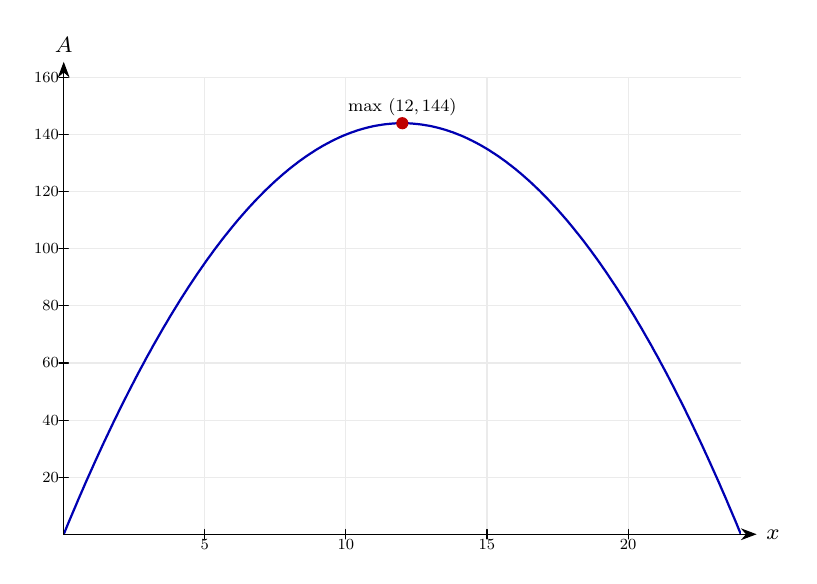
\begin{tikzpicture}[>={Stealth[length=2mm]},font=\footnotesize,line cap=round,line join=round]
\begin{scope}
\clip (0,0) rectangle (8.6,5.8);
\draw[gray!16] (0,0) grid[xstep=1.792,ystep=0.725] (8.6,5.8);
\draw[blue!70!black,thick] (0,0) -- (0.031,0.074) -- (0.061,0.148) -- (0.092,0.221) -- (0.123,0.294) -- (0.154,0.366) -- (0.184,0.438) -- (0.215,0.509) -- (0.246,0.58) -- (0.276,0.65) -- (0.307,0.719) -- (0.338,0.788) -- (0.369,0.857) -- (0.399,0.924) -- (0.43,0.992) -- (0.461,1.059) -- (0.491,1.125) -- (0.522,1.191) -- (0.553,1.256) -- (0.584,1.321) -- (0.614,1.385) -- (0.645,1.449) -- (0.676,1.512) -- (0.706,1.574) -- (0.737,1.636) -- (0.768,1.698) -- (0.799,1.759) -- (0.829,1.819) -- (0.86,1.879) -- (0.891,1.939) -- (0.921,1.997) -- (0.952,2.056) -- (0.983,2.114) -- (1.014,2.171) -- (1.044,2.228) -- (1.075,2.284) -- (1.106,2.339) -- (1.136,2.395) -- (1.167,2.449) -- (1.198,2.503) -- (1.229,2.557) -- (1.259,2.61) -- (1.29,2.662) -- (1.321,2.714) -- (1.351,2.766) -- (1.382,2.816) -- (1.413,2.867) -- (1.444,2.917) -- (1.474,2.966) -- (1.505,3.015) -- (1.536,3.063) -- (1.566,3.11) -- (1.597,3.158) -- (1.628,3.204) -- (1.659,3.25) -- (1.689,3.296) -- (1.72,3.341) -- (1.751,3.385) -- (1.781,3.429) -- (1.812,3.473) -- (1.843,3.516) -- (1.874,3.558) -- (1.904,3.6) -- (1.935,3.641) -- (1.966,3.682) -- (1.996,3.722) -- (2.027,3.762) -- (2.058,3.801) -- (2.089,3.839) -- (2.119,3.877) -- (2.15,3.915) -- (2.181,3.952) -- (2.211,3.989) -- (2.242,4.024) -- (2.273,4.06) -- (2.304,4.095) -- (2.334,4.129) -- (2.365,4.163) -- (2.396,4.196) -- (2.426,4.229) -- (2.457,4.261) -- (2.488,4.293) -- (2.519,4.324) -- (2.549,4.355) -- (2.58,4.385) -- (2.611,4.414) -- (2.641,4.443) -- (2.672,4.472) -- (2.703,4.5) -- (2.734,4.527) -- (2.764,4.554) -- (2.795,4.581) -- (2.826,4.606) -- (2.856,4.632) -- (2.887,4.656) -- (2.918,4.681) -- (2.949,4.704) -- (2.979,4.728) -- (3.01,4.75) -- (3.041,4.772) -- (3.071,4.794) -- (3.102,4.815) -- (3.133,4.835) -- (3.164,4.855) -- (3.194,4.875) -- (3.225,4.894) -- (3.256,4.912) -- (3.286,4.93) -- (3.317,4.947) -- (3.348,4.964) -- (3.379,4.98) -- (3.409,4.996) -- (3.44,5.011) -- (3.471,5.026) -- (3.501,5.04) -- (3.532,5.054) -- (3.563,5.067) -- (3.594,5.079) -- (3.624,5.091) -- (3.655,5.103) -- (3.686,5.113) -- (3.716,5.124) -- (3.747,5.134) -- (3.778,5.143) -- (3.809,5.152) -- (3.839,5.16) -- (3.87,5.168) -- (3.901,5.175) -- (3.931,5.182) -- (3.962,5.188) -- (3.993,5.193) -- (4.024,5.198) -- (4.054,5.203) -- (4.085,5.207) -- (4.116,5.21) -- (4.146,5.213) -- (4.177,5.216) -- (4.208,5.218) -- (4.239,5.219) -- (4.269,5.22) -- (4.3,5.22) -- (4.331,5.22) -- (4.361,5.219) -- (4.392,5.218) -- (4.423,5.216) -- (4.454,5.213) -- (4.484,5.21) -- (4.515,5.207) -- (4.546,5.203) -- (4.576,5.198) -- (4.607,5.193) -- (4.638,5.188) -- (4.669,5.182) -- (4.699,5.175) -- (4.73,5.168) -- (4.761,5.16) -- (4.791,5.152) -- (4.822,5.143) -- (4.853,5.134) -- (4.884,5.124) -- (4.914,5.113) -- (4.945,5.103) -- (4.976,5.091) -- (5.006,5.079) -- (5.037,5.067) -- (5.068,5.054) -- (5.099,5.04) -- (5.129,5.026) -- (5.16,5.011) -- (5.191,4.996) -- (5.221,4.98) -- (5.252,4.964) -- (5.283,4.947) -- (5.314,4.93) -- (5.344,4.912) -- (5.375,4.894) -- (5.406,4.875) -- (5.436,4.855) -- (5.467,4.835) -- (5.498,4.815) -- (5.529,4.794) -- (5.559,4.772) -- (5.59,4.75) -- (5.621,4.728) -- (5.651,4.704) -- (5.682,4.681) -- (5.713,4.656) -- (5.744,4.632) -- (5.774,4.606) -- (5.805,4.581) -- (5.836,4.554) -- (5.866,4.527) -- (5.897,4.5) -- (5.928,4.472) -- (5.959,4.443) -- (5.989,4.414) -- (6.02,4.385) -- (6.051,4.355) -- (6.081,4.324) -- (6.112,4.293) -- (6.143,4.261) -- (6.174,4.229) -- (6.204,4.196) -- (6.235,4.163) -- (6.266,4.129) -- (6.296,4.095) -- (6.327,4.06) -- (6.358,4.024) -- (6.389,3.989) -- (6.419,3.952) -- (6.45,3.915) -- (6.481,3.877) -- (6.511,3.839) -- (6.542,3.801) -- (6.573,3.762) -- (6.604,3.722) -- (6.634,3.682) -- (6.665,3.641) -- (6.696,3.6) -- (6.726,3.558) -- (6.757,3.516) -- (6.788,3.473) -- (6.819,3.429) -- (6.849,3.385) -- (6.88,3.341) -- (6.911,3.296) -- (6.941,3.25) -- (6.972,3.204) -- (7.003,3.158) -- (7.034,3.11) -- (7.064,3.063) -- (7.095,3.015) -- (7.126,2.966) -- (7.156,2.917) -- (7.187,2.867) -- (7.218,2.816) -- (7.249,2.766) -- (7.279,2.714) -- (7.31,2.662) -- (7.341,2.61) -- (7.371,2.557) -- (7.402,2.503) -- (7.433,2.449) -- (7.464,2.395) -- (7.494,2.339) -- (7.525,2.284) -- (7.556,2.228) -- (7.586,2.171) -- (7.617,2.114) -- (7.648,2.056) -- (7.679,1.997) -- (7.709,1.939) -- (7.74,1.879) -- (7.771,1.819) -- (7.801,1.759) -- (7.832,1.698) -- (7.863,1.636) -- (7.894,1.574) -- (7.924,1.512) -- (7.955,1.449) -- (7.986,1.385) -- (8.016,1.321) -- (8.047,1.256) -- (8.078,1.191) -- (8.109,1.125) -- (8.139,1.059) -- (8.17,0.992) -- (8.201,0.924) -- (8.231,0.857) -- (8.262,0.788) -- (8.293,0.719) -- (8.324,0.65) -- (8.354,0.58) -- (8.385,0.509) -- (8.416,0.438) -- (8.446,0.366) -- (8.477,0.294) -- (8.508,0.221) -- (8.539,0.148) -- (8.569,0.074) -- (8.6,0);
\end{scope}
\draw[->] (0,0) -- (8.8,0) node[right]{$x$};
\draw[->] (0,0) -- (0,6) node[above]{$A$};
\draw (1.792,-0.06) -- (1.792,0.06) node[below=1pt,scale=0.7]{$5$};
\draw (3.583,-0.06) -- (3.583,0.06) node[below=1pt,scale=0.7]{$10$};
\draw (5.375,-0.06) -- (5.375,0.06) node[below=1pt,scale=0.7]{$15$};
\draw (7.167,-0.06) -- (7.167,0.06) node[below=1pt,scale=0.7]{$20$};
\draw (-0.06,0.725) -- (0.06,0.725) node[left=1pt,scale=0.7]{$20$};
\draw (-0.06,1.45) -- (0.06,1.45) node[left=1pt,scale=0.7]{$40$};
\draw (-0.06,2.175) -- (0.06,2.175) node[left=1pt,scale=0.7]{$60$};
\draw (-0.06,2.9) -- (0.06,2.9) node[left=1pt,scale=0.7]{$80$};
\draw (-0.06,3.625) -- (0.06,3.625) node[left=1pt,scale=0.7]{$100$};
\draw (-0.06,4.35) -- (0.06,4.35) node[left=1pt,scale=0.7]{$120$};
\draw (-0.06,5.075) -- (0.06,5.075) node[left=1pt,scale=0.7]{$140$};
\draw (-0.06,5.8) -- (0.06,5.8) node[left=1pt,scale=0.7]{$160$};
\fill[red!75!black] (4.3,5.22) circle (2.2pt);
\node[above,scale=0.78] at (4.3,5.22) {max $(12,144)$};
\end{tikzpicture}
}
\end{center}
\small The model plotted against its variable, with the key point(s) marked.\normalsize

\medskip\hrule

\section*{Real-Life Problems 22\quad\small\texttt{(d5-022)}}
\addcontentsline{toc}{section}{Real-Life Problems 22 (d5-022)}
\textit{Difficulty: Foundation \quad\textbar\quad Marks: 6}

\question{A rectangular pen is built against a long straight wall (the wall forms one side). The pen uses \( 100 \) m of fencing for the remaining three sides, and the width of the pen (perpendicular to the wall) is \( x \) m. (a) Write down the length of the pen in terms of \( x \). (b) Show that the area is \( A = 100x - 2x^2 \). (c) Find the maximum area and the dimensions of the pen.}

\textbf{Worked solution.}

\textit{Step 1: (a) Three sides: two widths \( x \) and one length \( l \). So \( 2x + l = 100 \).}
\[\begin{gathered}
l = 100 - 2x
\end{gathered}\]
Rearrange to express \( l \) in terms of \( x \).

\textit{Step 2: (b) Area.}
\[\begin{gathered}
A = xl = x(100 - 2x) = 100x - 2x^2
\end{gathered}\]
Substitute \( l = 100 - 2x \).

\textit{Step 3: (c) Differentiate and set to zero.}
\[\begin{gathered}
\frac{\mathrm{d}A}{\mathrm{d}x} = 100 - 4x = 0 \implies x = 25 \text{ m}
\end{gathered}\]
Stationary point.

\textit{Step 4: Confirm maximum.}
\[\begin{gathered}
\frac{\mathrm{d}^2A}{\mathrm{d}x^2} = -4 < 0 \Rightarrow \text{maximum}
\end{gathered}\]
Negative second derivative.

\textit{Step 5: Maximum area.}
\[\begin{gathered}
l = 100 - 50 = 50 \text{ m}; \quad A = 25 \times 50 = 1250 \text{ m}^2
\end{gathered}\]
\( x = 25 \) m and \( l = 50 \) m.

\begin{answerbox}
\textbf{Final answer:}\quad (a) \(\displaystyle  l = 100 - 2x \) \\[3pt]  (b) Shown. \\[3pt]  (c) Width \(\displaystyle  = 25 \) m, length \(\displaystyle  = 50 \) m; max area \(\displaystyle  = 1250 \text{ m}^2 \)
\end{answerbox}
\textbf{Diagram.}

\begin{center}
\resizebox{\ifdim\width>\linewidth \linewidth\else \width\fi}{!}{%
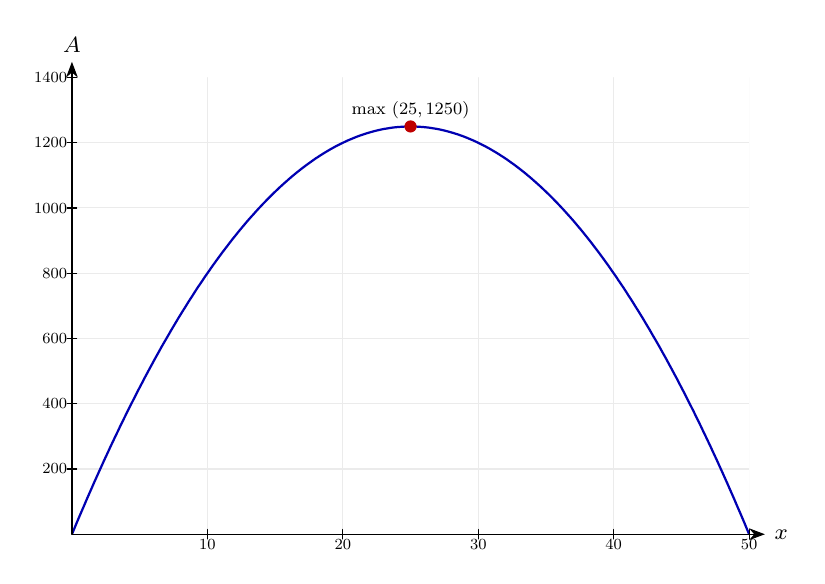
\begin{tikzpicture}[>={Stealth[length=2mm]},font=\footnotesize,line cap=round,line join=round]
\begin{scope}
\clip (0,0) rectangle (8.6,5.8);
\draw[gray!16] (0,0) grid[xstep=1.72,ystep=0.829] (8.6,5.8);
\draw[blue!70!black,thick] (0,0) -- (0.031,0.074) -- (0.061,0.147) -- (0.092,0.22) -- (0.123,0.292) -- (0.154,0.363) -- (0.184,0.434) -- (0.215,0.505) -- (0.246,0.575) -- (0.276,0.644) -- (0.307,0.713) -- (0.338,0.782) -- (0.369,0.85) -- (0.399,0.917) -- (0.43,0.984) -- (0.461,1.05) -- (0.491,1.116) -- (0.522,1.181) -- (0.553,1.246) -- (0.584,1.31) -- (0.614,1.374) -- (0.645,1.437) -- (0.676,1.5) -- (0.706,1.562) -- (0.737,1.623) -- (0.768,1.684) -- (0.799,1.745) -- (0.829,1.805) -- (0.86,1.864) -- (0.891,1.923) -- (0.921,1.982) -- (0.952,2.039) -- (0.983,2.097) -- (1.014,2.154) -- (1.044,2.21) -- (1.075,2.266) -- (1.106,2.321) -- (1.136,2.376) -- (1.167,2.43) -- (1.198,2.483) -- (1.229,2.536) -- (1.259,2.589) -- (1.29,2.641) -- (1.321,2.693) -- (1.351,2.744) -- (1.382,2.794) -- (1.413,2.844) -- (1.444,2.893) -- (1.474,2.942) -- (1.505,2.991) -- (1.536,3.038) -- (1.566,3.086) -- (1.597,3.133) -- (1.628,3.179) -- (1.659,3.224) -- (1.689,3.27) -- (1.72,3.314) -- (1.751,3.358) -- (1.781,3.402) -- (1.812,3.445) -- (1.843,3.488) -- (1.874,3.53) -- (1.904,3.571) -- (1.935,3.612) -- (1.966,3.652) -- (1.996,3.692) -- (2.027,3.732) -- (2.058,3.771) -- (2.089,3.809) -- (2.119,3.847) -- (2.15,3.884) -- (2.181,3.921) -- (2.211,3.957) -- (2.242,3.993) -- (2.273,4.028) -- (2.304,4.062) -- (2.334,4.096) -- (2.365,4.13) -- (2.396,4.163) -- (2.426,4.195) -- (2.457,4.227) -- (2.488,4.259) -- (2.519,4.29) -- (2.549,4.32) -- (2.58,4.35) -- (2.611,4.379) -- (2.641,4.408) -- (2.672,4.436) -- (2.703,4.464) -- (2.734,4.491) -- (2.764,4.518) -- (2.795,4.544) -- (2.826,4.57) -- (2.856,4.595) -- (2.887,4.619) -- (2.918,4.644) -- (2.949,4.667) -- (2.979,4.69) -- (3.01,4.712) -- (3.041,4.734) -- (3.071,4.756) -- (3.102,4.777) -- (3.133,4.797) -- (3.164,4.817) -- (3.194,4.836) -- (3.225,4.855) -- (3.256,4.873) -- (3.286,4.891) -- (3.317,4.908) -- (3.348,4.925) -- (3.379,4.941) -- (3.409,4.956) -- (3.44,4.971) -- (3.471,4.986) -- (3.501,5) -- (3.532,5.013) -- (3.563,5.026) -- (3.594,5.039) -- (3.624,5.051) -- (3.655,5.062) -- (3.686,5.073) -- (3.716,5.083) -- (3.747,5.093) -- (3.778,5.102) -- (3.809,5.111) -- (3.839,5.119) -- (3.87,5.127) -- (3.901,5.134) -- (3.931,5.141) -- (3.962,5.147) -- (3.993,5.152) -- (4.024,5.157) -- (4.054,5.162) -- (4.085,5.166) -- (4.116,5.169) -- (4.146,5.172) -- (4.177,5.174) -- (4.208,5.176) -- (4.239,5.178) -- (4.269,5.178) -- (4.3,5.179) -- (4.331,5.178) -- (4.361,5.178) -- (4.392,5.176) -- (4.423,5.174) -- (4.454,5.172) -- (4.484,5.169) -- (4.515,5.166) -- (4.546,5.162) -- (4.576,5.157) -- (4.607,5.152) -- (4.638,5.147) -- (4.669,5.141) -- (4.699,5.134) -- (4.73,5.127) -- (4.761,5.119) -- (4.791,5.111) -- (4.822,5.102) -- (4.853,5.093) -- (4.884,5.083) -- (4.914,5.073) -- (4.945,5.062) -- (4.976,5.051) -- (5.006,5.039) -- (5.037,5.026) -- (5.068,5.013) -- (5.099,5) -- (5.129,4.986) -- (5.16,4.971) -- (5.191,4.956) -- (5.221,4.941) -- (5.252,4.925) -- (5.283,4.908) -- (5.314,4.891) -- (5.344,4.873) -- (5.375,4.855) -- (5.406,4.836) -- (5.436,4.817) -- (5.467,4.797) -- (5.498,4.777) -- (5.529,4.756) -- (5.559,4.734) -- (5.59,4.712) -- (5.621,4.69) -- (5.651,4.667) -- (5.682,4.644) -- (5.713,4.619) -- (5.744,4.595) -- (5.774,4.57) -- (5.805,4.544) -- (5.836,4.518) -- (5.866,4.491) -- (5.897,4.464) -- (5.928,4.436) -- (5.959,4.408) -- (5.989,4.379) -- (6.02,4.35) -- (6.051,4.32) -- (6.081,4.29) -- (6.112,4.259) -- (6.143,4.227) -- (6.174,4.195) -- (6.204,4.163) -- (6.235,4.13) -- (6.266,4.096) -- (6.296,4.062) -- (6.327,4.028) -- (6.358,3.993) -- (6.389,3.957) -- (6.419,3.921) -- (6.45,3.884) -- (6.481,3.847) -- (6.511,3.809) -- (6.542,3.771) -- (6.573,3.732) -- (6.604,3.692) -- (6.634,3.652) -- (6.665,3.612) -- (6.696,3.571) -- (6.726,3.53) -- (6.757,3.488) -- (6.788,3.445) -- (6.819,3.402) -- (6.849,3.358) -- (6.88,3.314) -- (6.911,3.27) -- (6.941,3.224) -- (6.972,3.179) -- (7.003,3.133) -- (7.034,3.086) -- (7.064,3.038) -- (7.095,2.991) -- (7.126,2.942) -- (7.156,2.893) -- (7.187,2.844) -- (7.218,2.794) -- (7.249,2.744) -- (7.279,2.693) -- (7.31,2.641) -- (7.341,2.589) -- (7.371,2.536) -- (7.402,2.483) -- (7.433,2.43) -- (7.464,2.376) -- (7.494,2.321) -- (7.525,2.266) -- (7.556,2.21) -- (7.586,2.154) -- (7.617,2.097) -- (7.648,2.039) -- (7.679,1.982) -- (7.709,1.923) -- (7.74,1.864) -- (7.771,1.805) -- (7.801,1.745) -- (7.832,1.684) -- (7.863,1.623) -- (7.894,1.562) -- (7.924,1.5) -- (7.955,1.437) -- (7.986,1.374) -- (8.016,1.31) -- (8.047,1.246) -- (8.078,1.181) -- (8.109,1.116) -- (8.139,1.05) -- (8.17,0.984) -- (8.201,0.917) -- (8.231,0.85) -- (8.262,0.782) -- (8.293,0.713) -- (8.324,0.644) -- (8.354,0.575) -- (8.385,0.505) -- (8.416,0.434) -- (8.446,0.363) -- (8.477,0.292) -- (8.508,0.22) -- (8.539,0.147) -- (8.569,0.074) -- (8.6,0);
\end{scope}
\draw[->] (0,0) -- (8.8,0) node[right]{$x$};
\draw[->] (0,0) -- (0,6) node[above]{$A$};
\draw (1.72,-0.06) -- (1.72,0.06) node[below=1pt,scale=0.7]{$10$};
\draw (3.44,-0.06) -- (3.44,0.06) node[below=1pt,scale=0.7]{$20$};
\draw (5.16,-0.06) -- (5.16,0.06) node[below=1pt,scale=0.7]{$30$};
\draw (6.88,-0.06) -- (6.88,0.06) node[below=1pt,scale=0.7]{$40$};
\draw (8.6,-0.06) -- (8.6,0.06) node[below=1pt,scale=0.7]{$50$};
\draw (-0.06,0.829) -- (0.06,0.829) node[left=1pt,scale=0.7]{$200$};
\draw (-0.06,1.657) -- (0.06,1.657) node[left=1pt,scale=0.7]{$400$};
\draw (-0.06,2.486) -- (0.06,2.486) node[left=1pt,scale=0.7]{$600$};
\draw (-0.06,3.314) -- (0.06,3.314) node[left=1pt,scale=0.7]{$800$};
\draw (-0.06,4.143) -- (0.06,4.143) node[left=1pt,scale=0.7]{$1000$};
\draw (-0.06,4.971) -- (0.06,4.971) node[left=1pt,scale=0.7]{$1200$};
\draw (-0.06,5.8) -- (0.06,5.8) node[left=1pt,scale=0.7]{$1400$};
\fill[red!75!black] (4.3,5.179) circle (2.2pt);
\node[above,scale=0.78] at (4.3,5.179) {max $(25,1250)$};
\end{tikzpicture}
}
\end{center}
\small The model plotted against its variable, with the key point(s) marked.\normalsize

\medskip\hrule

\section*{Real-Life Problems 23\quad\small\texttt{(d5-023)}}
\addcontentsline{toc}{section}{Real-Life Problems 23 (d5-023)}
\textit{Difficulty: Foundation \quad\textbar\quad Marks: 5}

\question{A model rocket's height in metres after \( t \) seconds is \( h = -2t^3 + 18t^2 + 5 \) for \( 0 \leq t \leq 10 \). (a) Find the velocity \( \dfrac{\mathrm{d}h}{\mathrm{d}t} \). (b) Find the times when the rocket is neither ascending nor descending. (c) Find the maximum height.}

\textbf{Worked solution.}

\textit{Step 1: (a) Differentiate.}
\[\begin{gathered}
\frac{\mathrm{d}h}{\mathrm{d}t} = -6t^2 + 36t
\end{gathered}\]
Power rule.

\textit{Step 2: (b) Set velocity to zero.}
\[\begin{gathered}
-6t^2 + 36t = 0 \implies -6t(t - 6) = 0 \implies t = 0 \text{ or } t = 6
\end{gathered}\]
Factorise.

\textit{Step 3: (c) Maximum height at \( t = 6 \).}
\[\begin{gathered}
h(6) = -2(216) + 18(36) + 5 = -432 + 648 + 5 = 221 \text{ m}
\end{gathered}\]
Substitute \( t = 6 \) into \( h \). (\( t = 0 \) is launch, not a maximum.)

\begin{answerbox}
\textbf{Final answer:}\quad (a) \(\displaystyle  v = -6t^2 + 36t \) \\[3pt]  (b) \(\displaystyle  t = 0 \) and \(\displaystyle  t = 6 \) s \\[3pt]  (c) Maximum height \(\displaystyle  = 221 \) m
\end{answerbox}
\textbf{Diagram.}

\begin{center}
\resizebox{\ifdim\width>\linewidth \linewidth\else \width\fi}{!}{%
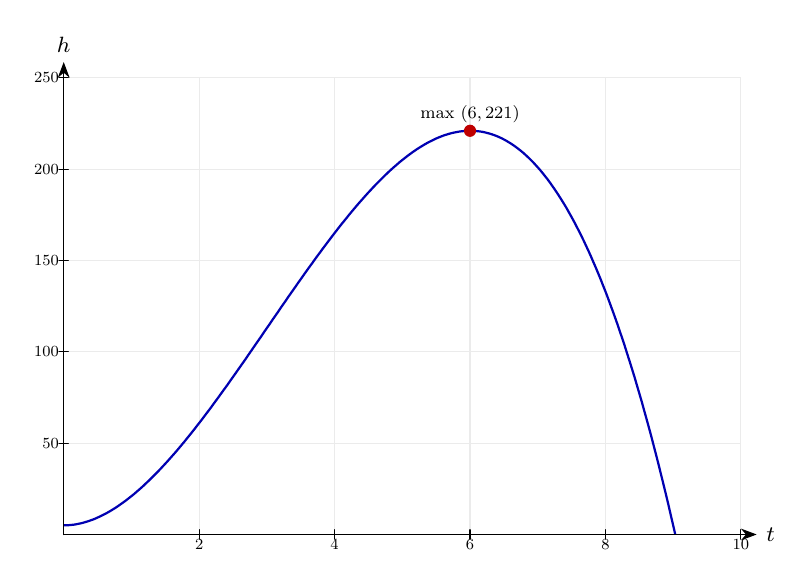
\begin{tikzpicture}[>={Stealth[length=2mm]},font=\footnotesize,line cap=round,line join=round]
\begin{scope}
\clip (0,0) rectangle (8.6,5.8);
\draw[gray!16] (0,0) grid[xstep=1.72,ystep=1.16] (8.6,5.8);
\draw[blue!70!black,thick] (0,0.116) -- (0.031,0.117) -- (0.061,0.118) -- (0.092,0.121) -- (0.123,0.124) -- (0.154,0.129) -- (0.184,0.135) -- (0.215,0.141) -- (0.246,0.149) -- (0.276,0.158) -- (0.307,0.167) -- (0.338,0.178) -- (0.369,0.189) -- (0.399,0.201) -- (0.43,0.215) -- (0.461,0.229) -- (0.491,0.244) -- (0.522,0.26) -- (0.553,0.276) -- (0.584,0.294) -- (0.614,0.312) -- (0.645,0.331) -- (0.676,0.351) -- (0.706,0.372) -- (0.737,0.394) -- (0.768,0.416) -- (0.799,0.439) -- (0.829,0.463) -- (0.86,0.487) -- (0.891,0.512) -- (0.921,0.538) -- (0.952,0.565) -- (0.983,0.592) -- (1.014,0.62) -- (1.044,0.649) -- (1.075,0.678) -- (1.106,0.708) -- (1.136,0.738) -- (1.167,0.769) -- (1.198,0.801) -- (1.229,0.833) -- (1.259,0.866) -- (1.29,0.899) -- (1.321,0.933) -- (1.351,0.967) -- (1.382,1.002) -- (1.413,1.037) -- (1.444,1.073) -- (1.474,1.109) -- (1.505,1.146) -- (1.536,1.183) -- (1.566,1.221) -- (1.597,1.259) -- (1.628,1.298) -- (1.659,1.336) -- (1.689,1.376) -- (1.72,1.415) -- (1.751,1.455) -- (1.781,1.495) -- (1.812,1.536) -- (1.843,1.577) -- (1.874,1.618) -- (1.904,1.66) -- (1.935,1.702) -- (1.966,1.744) -- (1.996,1.786) -- (2.027,1.829) -- (2.058,1.871) -- (2.089,1.914) -- (2.119,1.958) -- (2.15,2.001) -- (2.181,2.045) -- (2.211,2.088) -- (2.242,2.132) -- (2.273,2.176) -- (2.304,2.22) -- (2.334,2.265) -- (2.365,2.309) -- (2.396,2.354) -- (2.426,2.398) -- (2.457,2.443) -- (2.488,2.487) -- (2.519,2.532) -- (2.549,2.577) -- (2.58,2.622) -- (2.611,2.666) -- (2.641,2.711) -- (2.672,2.756) -- (2.703,2.8) -- (2.734,2.845) -- (2.764,2.89) -- (2.795,2.934) -- (2.826,2.978) -- (2.856,3.023) -- (2.887,3.067) -- (2.918,3.111) -- (2.949,3.155) -- (2.979,3.199) -- (3.01,3.242) -- (3.041,3.286) -- (3.071,3.329) -- (3.102,3.372) -- (3.133,3.415) -- (3.164,3.457) -- (3.194,3.5) -- (3.225,3.542) -- (3.256,3.583) -- (3.286,3.625) -- (3.317,3.666) -- (3.348,3.707) -- (3.379,3.748) -- (3.409,3.788) -- (3.44,3.828) -- (3.471,3.868) -- (3.501,3.907) -- (3.532,3.946) -- (3.563,3.984) -- (3.594,4.022) -- (3.624,4.06) -- (3.655,4.097) -- (3.686,4.134) -- (3.716,4.17) -- (3.747,4.206) -- (3.778,4.241) -- (3.809,4.276) -- (3.839,4.31) -- (3.87,4.344) -- (3.901,4.377) -- (3.931,4.41) -- (3.962,4.442) -- (3.993,4.474) -- (4.024,4.505) -- (4.054,4.535) -- (4.085,4.565) -- (4.116,4.595) -- (4.146,4.623) -- (4.177,4.651) -- (4.208,4.678) -- (4.239,4.705) -- (4.269,4.731) -- (4.3,4.756) -- (4.331,4.78) -- (4.361,4.804) -- (4.392,4.827) -- (4.423,4.85) -- (4.454,4.871) -- (4.484,4.892) -- (4.515,4.912) -- (4.546,4.931) -- (4.576,4.949) -- (4.607,4.967) -- (4.638,4.984) -- (4.669,4.999) -- (4.699,5.014) -- (4.73,5.029) -- (4.761,5.042) -- (4.791,5.054) -- (4.822,5.066) -- (4.853,5.076) -- (4.884,5.086) -- (4.914,5.094) -- (4.945,5.102) -- (4.976,5.108) -- (5.006,5.114) -- (5.037,5.119) -- (5.068,5.122) -- (5.099,5.125) -- (5.129,5.127) -- (5.16,5.127) -- (5.191,5.127) -- (5.221,5.125) -- (5.252,5.122) -- (5.283,5.119) -- (5.314,5.114) -- (5.344,5.108) -- (5.375,5.1) -- (5.406,5.092) -- (5.436,5.083) -- (5.467,5.072) -- (5.498,5.06) -- (5.529,5.047) -- (5.559,5.033) -- (5.59,5.017) -- (5.621,5) -- (5.651,4.982) -- (5.682,4.963) -- (5.713,4.942) -- (5.744,4.92) -- (5.774,4.897) -- (5.805,4.873) -- (5.836,4.847) -- (5.866,4.82) -- (5.897,4.791) -- (5.928,4.761) -- (5.959,4.73) -- (5.989,4.697) -- (6.02,4.663) -- (6.051,4.628) -- (6.081,4.591) -- (6.112,4.552) -- (6.143,4.513) -- (6.174,4.471) -- (6.204,4.428) -- (6.235,4.384) -- (6.266,4.338) -- (6.296,4.291) -- (6.327,4.242) -- (6.358,4.192) -- (6.389,4.14) -- (6.419,4.086) -- (6.45,4.031) -- (6.481,3.974) -- (6.511,3.916) -- (6.542,3.856) -- (6.573,3.794) -- (6.604,3.731) -- (6.634,3.666) -- (6.665,3.6) -- (6.696,3.531) -- (6.726,3.461) -- (6.757,3.39) -- (6.788,3.316) -- (6.819,3.241) -- (6.849,3.164) -- (6.88,3.086) -- (6.911,3.005) -- (6.941,2.923) -- (6.972,2.839) -- (7.003,2.753) -- (7.034,2.665) -- (7.064,2.576) -- (7.095,2.485) -- (7.126,2.391) -- (7.156,2.296) -- (7.187,2.199) -- (7.218,2.1) -- (7.249,2) -- (7.279,1.897) -- (7.31,1.792) -- (7.341,1.686) -- (7.371,1.577) -- (7.402,1.466) -- (7.433,1.354) -- (7.464,1.239) -- (7.494,1.123) -- (7.525,1.004) -- (7.556,0.883) -- (7.586,0.761) -- (7.617,0.636) -- (7.648,0.509) -- (7.679,0.38) -- (7.709,0.249) -- (7.74,0.116) -- (7.771,-0.019) -- (7.801,-0.157) -- (7.832,-0.296) -- (7.863,-0.438) -- (7.894,-0.582) -- (7.924,-0.728) -- (7.955,-0.877) -- (7.986,-1.027) -- (8.016,-1.18) -- (8.047,-1.335) -- (8.078,-1.492) -- (8.109,-1.652) -- (8.139,-1.814) -- (8.17,-1.978) -- (8.201,-2.144) -- (8.231,-2.313) -- (8.262,-2.484) -- (8.293,-2.658) -- (8.324,-2.833) -- (8.354,-3.012) -- (8.385,-3.192) -- (8.416,-3.375) -- (8.446,-3.561) -- (8.477,-3.748) -- (8.508,-3.939) -- (8.539,-4.131) -- (8.569,-4.326) -- (8.6,-4.524);
\end{scope}
\draw[->] (0,0) -- (8.8,0) node[right]{$t$};
\draw[->] (0,0) -- (0,6) node[above]{$h$};
\draw (1.72,-0.06) -- (1.72,0.06) node[below=1pt,scale=0.7]{$2$};
\draw (3.44,-0.06) -- (3.44,0.06) node[below=1pt,scale=0.7]{$4$};
\draw (5.16,-0.06) -- (5.16,0.06) node[below=1pt,scale=0.7]{$6$};
\draw (6.88,-0.06) -- (6.88,0.06) node[below=1pt,scale=0.7]{$8$};
\draw (8.6,-0.06) -- (8.6,0.06) node[below=1pt,scale=0.7]{$10$};
\draw (-0.06,1.16) -- (0.06,1.16) node[left=1pt,scale=0.7]{$50$};
\draw (-0.06,2.32) -- (0.06,2.32) node[left=1pt,scale=0.7]{$100$};
\draw (-0.06,3.48) -- (0.06,3.48) node[left=1pt,scale=0.7]{$150$};
\draw (-0.06,4.64) -- (0.06,4.64) node[left=1pt,scale=0.7]{$200$};
\draw (-0.06,5.8) -- (0.06,5.8) node[left=1pt,scale=0.7]{$250$};
\fill[red!75!black] (5.16,5.127) circle (2.2pt);
\node[above,scale=0.78] at (5.16,5.127) {max $(6,221)$};
\end{tikzpicture}
}
\end{center}
\small The model plotted against its variable, with the key point(s) marked.\normalsize

\medskip\hrule

\section*{Real-Life Problems 24\quad\small\texttt{(d5-024)}}
\addcontentsline{toc}{section}{Real-Life Problems 24 (d5-024)}
\textit{Difficulty: Foundation \quad\textbar\quad Marks: 6}

\question{A piece of wire 60 cm long is cut into two pieces. One piece is bent into a square of side \( x \) cm and the other into a rectangle of dimensions \( 2x \) cm by \( y \) cm. (a) Write an expression for \( y \) in terms of \( x \). (b) Find the total area \( A \) of both shapes in terms of \( x \). (c) Use calculus to find the value of \( x \) that minimises the total area.}

\textbf{Worked solution.}

\textit{Step 1: (a) Total wire: perimeter of square + perimeter of rectangle \( = 60 \).}
\[\begin{gathered}
4x + 2(2x + y) = 60 \implies 4x + 4x + 2y = 60 \implies y = 30 - 4x
\end{gathered}\]
Perimeter of rectangle \( = 2(2x + y) \).

\textit{Step 2: (b) Total area.}
\[\begin{gathered}
A = x^2 + 2x \cdot y = x^2 + 2x(30 - 4x) = x^2 + 60x - 8x^2 = -7x^2 + 60x
\end{gathered}\]
Area of square \( = x^2 \); area of rectangle \( = 2xy \).

\textit{Step 3: (c) Differentiate.}
\[\begin{gathered}
\frac{\mathrm{d}A}{\mathrm{d}x} = -14x + 60 = 0 \implies x = \frac{60}{14} = \frac{30}{7} \approx 4.29 \text{ cm}
\end{gathered}\]
Set derivative to zero and solve.

\textit{Step 4: Confirm minimum.}
\[\begin{gathered}
\frac{\mathrm{d}^2A}{\mathrm{d}x^2} = -14 < 0
\end{gathered}\]
Wait --- negative second derivative means this is a maximum, not a minimum! The area function is a downward parabola, so it has a maximum at \( x = \tfrac{30}{7} \). For a minimum of a downward parabola on a restricted domain, check the endpoints. \( x \) must satisfy \( y = 30 - 4x \geq 0 \), so \( x \leq 7.5 \), and \( x > 0 \). The minimum area occurs at an endpoint of the domain.

\textit{Step 5: Check endpoints.}
\[\begin{gathered}
A(0) = 0; \quad A(7.5) = -7(56.25) + 60(7.5) = -393.75 + 450 = 56.25 \text{ cm}^2
\end{gathered}\]
The minimum total area is 0 cm\(^2\) (degenerate case at \(x = 0\)). Minimum non-degenerate area is at \( x \to 0^+ \). The stationary point \( x \approx 4.29 \) gives the maximum area of about \( 128.6 \text{ cm}^2 \).

\begin{answerbox}
\textbf{Final answer:}\quad (a) \(\displaystyle  y = 30 - 4x \) \\[3pt]  (b) \(\displaystyle  A = -7x^2 + 60x \) \\[3pt]  (c) The stationary point \(\displaystyle  x = \tfrac{30}{7} \) is a maximum (\(\displaystyle  \approx 128.6 \text{ cm}^2 \)); area is minimised at the domain boundaries.
\end{answerbox}
\textbf{Diagram.}

\begin{center}
\resizebox{\ifdim\width>\linewidth \linewidth\else \width\fi}{!}{%
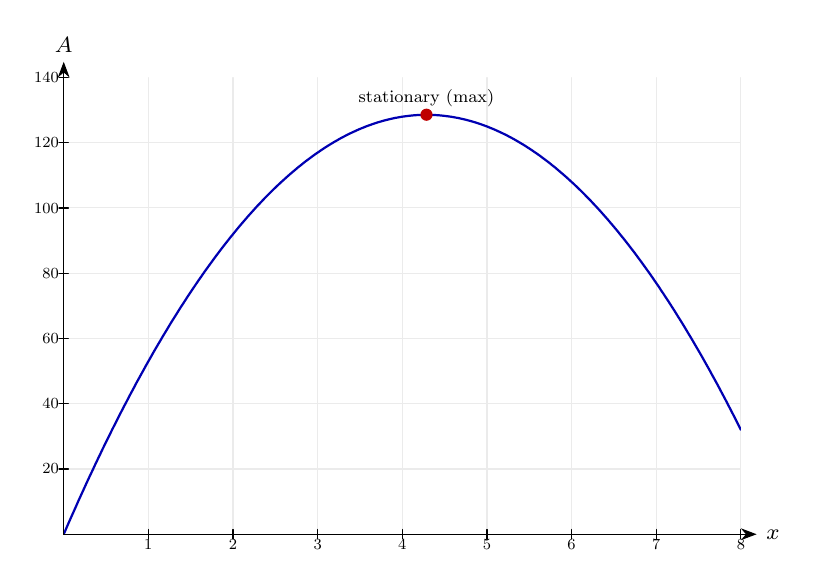
\begin{tikzpicture}[>={Stealth[length=2mm]},font=\footnotesize,line cap=round,line join=round]
\begin{scope}
\clip (0,0) rectangle (8.6,5.8);
\draw[gray!16] (0,0) grid[xstep=1.075,ystep=0.829] (8.6,5.8);
\draw[blue!70!black,thick] (0,0) -- (0.031,0.071) -- (0.061,0.141) -- (0.092,0.211) -- (0.123,0.28) -- (0.154,0.349) -- (0.184,0.418) -- (0.215,0.486) -- (0.246,0.553) -- (0.276,0.62) -- (0.307,0.687) -- (0.338,0.753) -- (0.369,0.818) -- (0.399,0.883) -- (0.43,0.948) -- (0.461,1.012) -- (0.491,1.076) -- (0.522,1.139) -- (0.553,1.202) -- (0.584,1.264) -- (0.614,1.326) -- (0.645,1.387) -- (0.676,1.448) -- (0.706,1.508) -- (0.737,1.568) -- (0.768,1.628) -- (0.799,1.686) -- (0.829,1.745) -- (0.86,1.803) -- (0.891,1.86) -- (0.921,1.918) -- (0.952,1.974) -- (0.983,2.03) -- (1.014,2.086) -- (1.044,2.141) -- (1.075,2.196) -- (1.106,2.25) -- (1.136,2.304) -- (1.167,2.357) -- (1.198,2.41) -- (1.229,2.462) -- (1.259,2.514) -- (1.29,2.565) -- (1.321,2.616) -- (1.351,2.667) -- (1.382,2.717) -- (1.413,2.766) -- (1.444,2.815) -- (1.474,2.864) -- (1.505,2.912) -- (1.536,2.959) -- (1.566,3.006) -- (1.597,3.053) -- (1.628,3.099) -- (1.659,3.145) -- (1.689,3.19) -- (1.72,3.235) -- (1.751,3.279) -- (1.781,3.323) -- (1.812,3.366) -- (1.843,3.409) -- (1.874,3.451) -- (1.904,3.493) -- (1.935,3.535) -- (1.966,3.576) -- (1.996,3.616) -- (2.027,3.656) -- (2.058,3.696) -- (2.089,3.735) -- (2.119,3.773) -- (2.15,3.811) -- (2.181,3.849) -- (2.211,3.886) -- (2.242,3.923) -- (2.273,3.959) -- (2.304,3.995) -- (2.334,4.03) -- (2.365,4.065) -- (2.396,4.099) -- (2.426,4.133) -- (2.457,4.167) -- (2.488,4.199) -- (2.519,4.232) -- (2.549,4.264) -- (2.58,4.295) -- (2.611,4.326) -- (2.641,4.357) -- (2.672,4.387) -- (2.703,4.417) -- (2.734,4.446) -- (2.764,4.474) -- (2.795,4.502) -- (2.826,4.53) -- (2.856,4.557) -- (2.887,4.584) -- (2.918,4.61) -- (2.949,4.636) -- (2.979,4.662) -- (3.01,4.686) -- (3.041,4.711) -- (3.071,4.735) -- (3.102,4.758) -- (3.133,4.781) -- (3.164,4.804) -- (3.194,4.826) -- (3.225,4.847) -- (3.256,4.868) -- (3.286,4.889) -- (3.317,4.909) -- (3.348,4.929) -- (3.379,4.948) -- (3.409,4.966) -- (3.44,4.985) -- (3.471,5.002) -- (3.501,5.02) -- (3.532,5.037) -- (3.563,5.053) -- (3.594,5.069) -- (3.624,5.084) -- (3.655,5.099) -- (3.686,5.113) -- (3.716,5.127) -- (3.747,5.141) -- (3.778,5.154) -- (3.809,5.166) -- (3.839,5.179) -- (3.87,5.19) -- (3.901,5.201) -- (3.931,5.212) -- (3.962,5.222) -- (3.993,5.232) -- (4.024,5.241) -- (4.054,5.25) -- (4.085,5.258) -- (4.116,5.266) -- (4.146,5.273) -- (4.177,5.28) -- (4.208,5.287) -- (4.239,5.292) -- (4.269,5.298) -- (4.3,5.303) -- (4.331,5.307) -- (4.361,5.311) -- (4.392,5.315) -- (4.423,5.318) -- (4.454,5.321) -- (4.484,5.323) -- (4.515,5.324) -- (4.546,5.326) -- (4.576,5.326) -- (4.607,5.327) -- (4.638,5.326) -- (4.669,5.326) -- (4.699,5.324) -- (4.73,5.323) -- (4.761,5.321) -- (4.791,5.318) -- (4.822,5.315) -- (4.853,5.311) -- (4.884,5.307) -- (4.914,5.303) -- (4.945,5.298) -- (4.976,5.292) -- (5.006,5.287) -- (5.037,5.28) -- (5.068,5.273) -- (5.099,5.266) -- (5.129,5.258) -- (5.16,5.25) -- (5.191,5.241) -- (5.221,5.232) -- (5.252,5.222) -- (5.283,5.212) -- (5.314,5.201) -- (5.344,5.19) -- (5.375,5.179) -- (5.406,5.166) -- (5.436,5.154) -- (5.467,5.141) -- (5.498,5.127) -- (5.529,5.113) -- (5.559,5.099) -- (5.59,5.084) -- (5.621,5.069) -- (5.651,5.053) -- (5.682,5.037) -- (5.713,5.02) -- (5.744,5.002) -- (5.774,4.985) -- (5.805,4.966) -- (5.836,4.948) -- (5.866,4.929) -- (5.897,4.909) -- (5.928,4.889) -- (5.959,4.868) -- (5.989,4.847) -- (6.02,4.826) -- (6.051,4.804) -- (6.081,4.781) -- (6.112,4.758) -- (6.143,4.735) -- (6.174,4.711) -- (6.204,4.686) -- (6.235,4.662) -- (6.266,4.636) -- (6.296,4.61) -- (6.327,4.584) -- (6.358,4.557) -- (6.389,4.53) -- (6.419,4.502) -- (6.45,4.474) -- (6.481,4.446) -- (6.511,4.417) -- (6.542,4.387) -- (6.573,4.357) -- (6.604,4.326) -- (6.634,4.295) -- (6.665,4.264) -- (6.696,4.232) -- (6.726,4.199) -- (6.757,4.167) -- (6.788,4.133) -- (6.819,4.099) -- (6.849,4.065) -- (6.88,4.03) -- (6.911,3.995) -- (6.941,3.959) -- (6.972,3.923) -- (7.003,3.886) -- (7.034,3.849) -- (7.064,3.811) -- (7.095,3.773) -- (7.126,3.735) -- (7.156,3.696) -- (7.187,3.656) -- (7.218,3.616) -- (7.249,3.576) -- (7.279,3.535) -- (7.31,3.493) -- (7.341,3.451) -- (7.371,3.409) -- (7.402,3.366) -- (7.433,3.323) -- (7.464,3.279) -- (7.494,3.235) -- (7.525,3.19) -- (7.556,3.145) -- (7.586,3.099) -- (7.617,3.053) -- (7.648,3.006) -- (7.679,2.959) -- (7.709,2.912) -- (7.74,2.864) -- (7.771,2.815) -- (7.801,2.766) -- (7.832,2.717) -- (7.863,2.667) -- (7.894,2.616) -- (7.924,2.565) -- (7.955,2.514) -- (7.986,2.462) -- (8.016,2.41) -- (8.047,2.357) -- (8.078,2.304) -- (8.109,2.25) -- (8.139,2.196) -- (8.17,2.141) -- (8.201,2.086) -- (8.231,2.03) -- (8.262,1.974) -- (8.293,1.918) -- (8.324,1.86) -- (8.354,1.803) -- (8.385,1.745) -- (8.416,1.686) -- (8.446,1.628) -- (8.477,1.568) -- (8.508,1.508) -- (8.539,1.448) -- (8.569,1.387) -- (8.6,1.326);
\end{scope}
\draw[->] (0,0) -- (8.8,0) node[right]{$x$};
\draw[->] (0,0) -- (0,6) node[above]{$A$};
\draw (1.075,-0.06) -- (1.075,0.06) node[below=1pt,scale=0.7]{$1$};
\draw (2.15,-0.06) -- (2.15,0.06) node[below=1pt,scale=0.7]{$2$};
\draw (3.225,-0.06) -- (3.225,0.06) node[below=1pt,scale=0.7]{$3$};
\draw (4.3,-0.06) -- (4.3,0.06) node[below=1pt,scale=0.7]{$4$};
\draw (5.375,-0.06) -- (5.375,0.06) node[below=1pt,scale=0.7]{$5$};
\draw (6.45,-0.06) -- (6.45,0.06) node[below=1pt,scale=0.7]{$6$};
\draw (7.525,-0.06) -- (7.525,0.06) node[below=1pt,scale=0.7]{$7$};
\draw (8.6,-0.06) -- (8.6,0.06) node[below=1pt,scale=0.7]{$8$};
\draw (-0.06,0.829) -- (0.06,0.829) node[left=1pt,scale=0.7]{$20$};
\draw (-0.06,1.657) -- (0.06,1.657) node[left=1pt,scale=0.7]{$40$};
\draw (-0.06,2.486) -- (0.06,2.486) node[left=1pt,scale=0.7]{$60$};
\draw (-0.06,3.314) -- (0.06,3.314) node[left=1pt,scale=0.7]{$80$};
\draw (-0.06,4.143) -- (0.06,4.143) node[left=1pt,scale=0.7]{$100$};
\draw (-0.06,4.971) -- (0.06,4.971) node[left=1pt,scale=0.7]{$120$};
\draw (-0.06,5.8) -- (0.06,5.8) node[left=1pt,scale=0.7]{$140$};
\fill[red!75!black] (4.607,5.328) circle (2.2pt);
\node[above,scale=0.78] at (4.607,5.328) {stationary (max)};
\end{tikzpicture}
}
\end{center}
\small The model plotted against its variable, with the key point(s) marked.\normalsize

\medskip\hrule

\section*{Real-Life Problems 25\quad\small\texttt{(d5-025)}}
\addcontentsline{toc}{section}{Real-Life Problems 25 (d5-025)}
\textit{Difficulty: Foundation \quad\textbar\quad Marks: 7}

\question{A closed rectangular box has a square base of side \( x \) cm and height \( h \) cm. The total surface area is \( 150 \) cm\(^2\). (a) Show that the volume is \( V = \dfrac{150x - 2x^3}{4} \). (b) Find the value of \( x \) that maximises the volume.}

\textbf{Worked solution.}

\textit{Step 1: (a) Surface area: 2 square faces + 4 rectangular faces.}
\[\begin{gathered}
2x^2 + 4xh = 150 \implies h = \frac{150 - 2x^2}{4x}
\end{gathered}\]
Rearrange to express \( h \) in terms of \( x \).

\textit{Step 2: Volume.}
\[\begin{gathered}
V = x^2 h = x^2 \cdot \frac{150 - 2x^2}{4x} = \frac{x(150 - 2x^2)}{4} = \frac{150x - 2x^3}{4}
\end{gathered}\]
Substitute \( h \) into \( V = x^2 h \).

\textit{Step 3: (b) Differentiate.}
\[\begin{gathered}
\frac{\mathrm{d}V}{\mathrm{d}x} = \frac{150 - 6x^2}{4}
\end{gathered}\]
Power rule applied inside the fraction.

\textit{Step 4: Set to zero.}
\[\begin{gathered}
150 - 6x^2 = 0 \implies x^2 = 25 \implies x = 5 \text{ cm}
\end{gathered}\]
Take the positive root since \( x > 0 \).

\textit{Step 5: Confirm maximum.}
\[\begin{gathered}
\frac{\mathrm{d}^2V}{\mathrm{d}x^2} = \frac{-12x}{4} = -3x; \quad x=5: -15 < 0 \Rightarrow \text{maximum}
\end{gathered}\]
Negative second derivative at \( x = 5 \).

\begin{answerbox}
\textbf{Final answer:}\quad (a) Shown. \\[3pt]  (b) \(\displaystyle  x = 5 \) cm
\end{answerbox}
\textbf{Diagram.}

\begin{center}
\resizebox{\ifdim\width>\linewidth \linewidth\else \width\fi}{!}{%
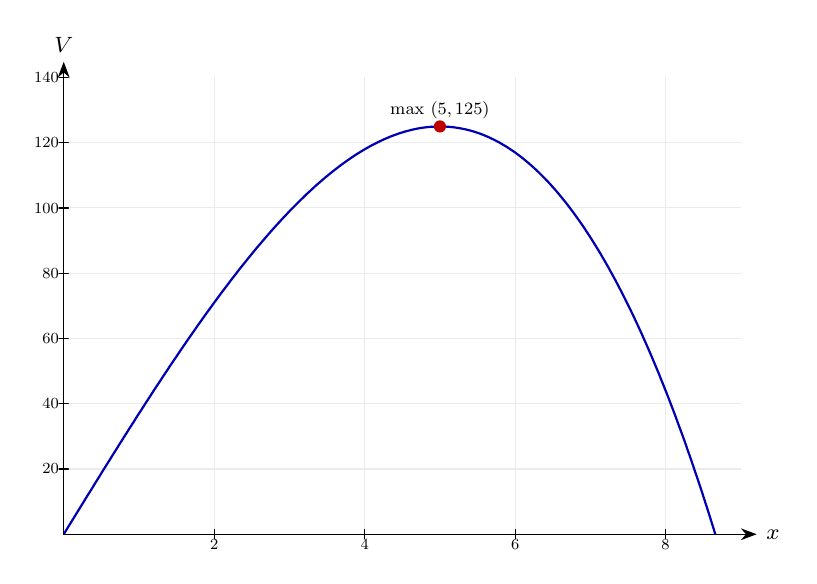
\begin{tikzpicture}[>={Stealth[length=2mm]},font=\footnotesize,line cap=round,line join=round]
\begin{scope}
\clip (0,0) rectangle (8.6,5.8);
\draw[gray!16] (0,0) grid[xstep=1.911,ystep=0.829] (8.6,5.8);
\draw[blue!70!black,thick] (0,0) -- (0.031,0.05) -- (0.061,0.1) -- (0.092,0.15) -- (0.123,0.2) -- (0.154,0.25) -- (0.184,0.299) -- (0.215,0.349) -- (0.246,0.399) -- (0.276,0.449) -- (0.307,0.499) -- (0.338,0.548) -- (0.369,0.598) -- (0.399,0.648) -- (0.43,0.697) -- (0.461,0.747) -- (0.491,0.796) -- (0.522,0.846) -- (0.553,0.895) -- (0.584,0.944) -- (0.614,0.993) -- (0.645,1.042) -- (0.676,1.091) -- (0.706,1.14) -- (0.737,1.189) -- (0.768,1.238) -- (0.799,1.286) -- (0.829,1.335) -- (0.86,1.383) -- (0.891,1.431) -- (0.921,1.48) -- (0.952,1.528) -- (0.983,1.575) -- (1.014,1.623) -- (1.044,1.671) -- (1.075,1.718) -- (1.106,1.766) -- (1.136,1.813) -- (1.167,1.86) -- (1.198,1.907) -- (1.229,1.953) -- (1.259,2) -- (1.29,2.046) -- (1.321,2.093) -- (1.351,2.139) -- (1.382,2.184) -- (1.413,2.23) -- (1.444,2.276) -- (1.474,2.321) -- (1.505,2.366) -- (1.536,2.411) -- (1.566,2.455) -- (1.597,2.5) -- (1.628,2.544) -- (1.659,2.588) -- (1.689,2.632) -- (1.72,2.676) -- (1.751,2.719) -- (1.781,2.762) -- (1.812,2.805) -- (1.843,2.848) -- (1.874,2.89) -- (1.904,2.932) -- (1.935,2.974) -- (1.966,3.016) -- (1.996,3.057) -- (2.027,3.098) -- (2.058,3.139) -- (2.089,3.179) -- (2.119,3.22) -- (2.15,3.26) -- (2.181,3.299) -- (2.211,3.339) -- (2.242,3.378) -- (2.273,3.417) -- (2.304,3.455) -- (2.334,3.493) -- (2.365,3.531) -- (2.396,3.569) -- (2.426,3.606) -- (2.457,3.643) -- (2.488,3.679) -- (2.519,3.715) -- (2.549,3.751) -- (2.58,3.787) -- (2.611,3.822) -- (2.641,3.857) -- (2.672,3.891) -- (2.703,3.926) -- (2.734,3.959) -- (2.764,3.993) -- (2.795,4.026) -- (2.826,4.058) -- (2.856,4.091) -- (2.887,4.123) -- (2.918,4.154) -- (2.949,4.185) -- (2.979,4.216) -- (3.01,4.246) -- (3.041,4.276) -- (3.071,4.306) -- (3.102,4.335) -- (3.133,4.363) -- (3.164,4.392) -- (3.194,4.42) -- (3.225,4.447) -- (3.256,4.474) -- (3.286,4.5) -- (3.317,4.527) -- (3.348,4.552) -- (3.379,4.577) -- (3.409,4.602) -- (3.44,4.626) -- (3.471,4.65) -- (3.501,4.674) -- (3.532,4.696) -- (3.563,4.719) -- (3.594,4.741) -- (3.624,4.762) -- (3.655,4.783) -- (3.686,4.804) -- (3.716,4.824) -- (3.747,4.843) -- (3.778,4.862) -- (3.809,4.881) -- (3.839,4.898) -- (3.87,4.916) -- (3.901,4.933) -- (3.931,4.949) -- (3.962,4.965) -- (3.993,4.98) -- (4.024,4.995) -- (4.054,5.009) -- (4.085,5.023) -- (4.116,5.036) -- (4.146,5.049) -- (4.177,5.061) -- (4.208,5.072) -- (4.239,5.083) -- (4.269,5.094) -- (4.3,5.103) -- (4.331,5.113) -- (4.361,5.121) -- (4.392,5.129) -- (4.423,5.137) -- (4.454,5.144) -- (4.484,5.15) -- (4.515,5.156) -- (4.546,5.161) -- (4.576,5.165) -- (4.607,5.169) -- (4.638,5.172) -- (4.669,5.175) -- (4.699,5.176) -- (4.73,5.178) -- (4.761,5.178) -- (4.791,5.179) -- (4.822,5.178) -- (4.853,5.177) -- (4.884,5.175) -- (4.914,5.172) -- (4.945,5.169) -- (4.976,5.165) -- (5.006,5.16) -- (5.037,5.155) -- (5.068,5.149) -- (5.099,5.143) -- (5.129,5.135) -- (5.16,5.128) -- (5.191,5.119) -- (5.221,5.11) -- (5.252,5.099) -- (5.283,5.089) -- (5.314,5.077) -- (5.344,5.065) -- (5.375,5.052) -- (5.406,5.039) -- (5.436,5.024) -- (5.467,5.009) -- (5.498,4.993) -- (5.529,4.977) -- (5.559,4.959) -- (5.59,4.941) -- (5.621,4.923) -- (5.651,4.903) -- (5.682,4.883) -- (5.713,4.862) -- (5.744,4.84) -- (5.774,4.817) -- (5.805,4.794) -- (5.836,4.77) -- (5.866,4.745) -- (5.897,4.719) -- (5.928,4.692) -- (5.959,4.665) -- (5.989,4.637) -- (6.02,4.608) -- (6.051,4.578) -- (6.081,4.548) -- (6.112,4.516) -- (6.143,4.484) -- (6.174,4.451) -- (6.204,4.417) -- (6.235,4.383) -- (6.266,4.347) -- (6.296,4.311) -- (6.327,4.273) -- (6.358,4.235) -- (6.389,4.196) -- (6.419,4.157) -- (6.45,4.116) -- (6.481,4.074) -- (6.511,4.032) -- (6.542,3.989) -- (6.573,3.945) -- (6.604,3.9) -- (6.634,3.854) -- (6.665,3.807) -- (6.696,3.759) -- (6.726,3.711) -- (6.757,3.661) -- (6.788,3.611) -- (6.819,3.56) -- (6.849,3.507) -- (6.88,3.454) -- (6.911,3.4) -- (6.941,3.345) -- (6.972,3.289) -- (7.003,3.232) -- (7.034,3.174) -- (7.064,3.116) -- (7.095,3.056) -- (7.126,2.995) -- (7.156,2.934) -- (7.187,2.871) -- (7.218,2.808) -- (7.249,2.743) -- (7.279,2.678) -- (7.31,2.611) -- (7.341,2.544) -- (7.371,2.475) -- (7.402,2.406) -- (7.433,2.335) -- (7.464,2.264) -- (7.494,2.192) -- (7.525,2.118) -- (7.556,2.044) -- (7.586,1.968) -- (7.617,1.892) -- (7.648,1.814) -- (7.679,1.736) -- (7.709,1.656) -- (7.74,1.576) -- (7.771,1.494) -- (7.801,1.411) -- (7.832,1.327) -- (7.863,1.243) -- (7.894,1.157) -- (7.924,1.07) -- (7.955,0.982) -- (7.986,0.893) -- (8.016,0.803) -- (8.047,0.712) -- (8.078,0.619) -- (8.109,0.526) -- (8.139,0.432) -- (8.17,0.336) -- (8.201,0.239) -- (8.231,0.142) -- (8.262,0.043) -- (8.293,-0.057) -- (8.324,-0.158) -- (8.354,-0.26) -- (8.385,-0.364) -- (8.416,-0.468) -- (8.446,-0.574) -- (8.477,-0.68) -- (8.508,-0.788) -- (8.539,-0.897) -- (8.569,-1.007) -- (8.6,-1.119);
\end{scope}
\draw[->] (0,0) -- (8.8,0) node[right]{$x$};
\draw[->] (0,0) -- (0,6) node[above]{$V$};
\draw (1.911,-0.06) -- (1.911,0.06) node[below=1pt,scale=0.7]{$2$};
\draw (3.822,-0.06) -- (3.822,0.06) node[below=1pt,scale=0.7]{$4$};
\draw (5.733,-0.06) -- (5.733,0.06) node[below=1pt,scale=0.7]{$6$};
\draw (7.644,-0.06) -- (7.644,0.06) node[below=1pt,scale=0.7]{$8$};
\draw (-0.06,0.829) -- (0.06,0.829) node[left=1pt,scale=0.7]{$20$};
\draw (-0.06,1.657) -- (0.06,1.657) node[left=1pt,scale=0.7]{$40$};
\draw (-0.06,2.486) -- (0.06,2.486) node[left=1pt,scale=0.7]{$60$};
\draw (-0.06,3.314) -- (0.06,3.314) node[left=1pt,scale=0.7]{$80$};
\draw (-0.06,4.143) -- (0.06,4.143) node[left=1pt,scale=0.7]{$100$};
\draw (-0.06,4.971) -- (0.06,4.971) node[left=1pt,scale=0.7]{$120$};
\draw (-0.06,5.8) -- (0.06,5.8) node[left=1pt,scale=0.7]{$140$};
\fill[red!75!black] (4.778,5.179) circle (2.2pt);
\node[above,scale=0.78] at (4.778,5.179) {max $(5,125)$};
\end{tikzpicture}
}
\end{center}
\small The model plotted against its variable, with the key point(s) marked.\normalsize

\medskip\hrule

\section*{Real-Life Problems 26\quad\small\texttt{(d5-026)}}
\addcontentsline{toc}{section}{Real-Life Problems 26 (d5-026)}
\textit{Difficulty: Foundation \quad\textbar\quad Marks: 6}

\question{A particle moves along a straight line. The displacement from the origin after \( t \) seconds is \( s = 6t - t^2 \) m for \( 0 \leq t \leq 8 \). (a) Find the velocity when \( t = 1 \). (b) Find the displacement at the instant when the particle is momentarily at rest. (c) Find the total distance travelled in the first 8 seconds.}

\textbf{Worked solution.}

\textit{Step 1: (a) Differentiate.}
\[\begin{gathered}
v = \frac{\mathrm{d}s}{\mathrm{d}t} = 6 - 2t; \quad v(1) = 6 - 2 = 4 \text{ ms}^{-1}
\end{gathered}\]
Power rule, then substitute \( t = 1 \).

\textit{Step 2: (b) Particle at rest: \( v = 0 \).}
\[\begin{gathered}
6 - 2t = 0 \implies t = 3 \text{ s}; \quad s(3) = 18 - 9 = 9 \text{ m}
\end{gathered}\]
Substitute \( t = 3 \) into \( s \).

\textit{Step 3: (c) After \( t = 3 \), the particle reverses. Find \( s(8) \).}
\[\begin{gathered}
s(8) = 48 - 64 = -16 \text{ m}
\end{gathered}\]
The particle is now 16 m on the other side of the origin.

\textit{Step 4: Total distance.}
\[\begin{gathered}
d = 9 + (9 - (-16)) = 9 + 25 = 34 \text{ m}
\end{gathered}\]
Outward journey: 9 m. Return journey: from \( s = 9 \) to \( s = -16 \) is \( 25 \) m.

\begin{answerbox}
\textbf{Final answer:}\quad (a) \(\displaystyle  4 \text{ ms}^{-1} \) \\[3pt]  (b) \(\displaystyle  9 \) m from origin \\[3pt]  (c) Total distance \(\displaystyle  = 34 \) m
\end{answerbox}
\textbf{Diagram.}

\begin{center}
\resizebox{\ifdim\width>\linewidth \linewidth\else \width\fi}{!}{%
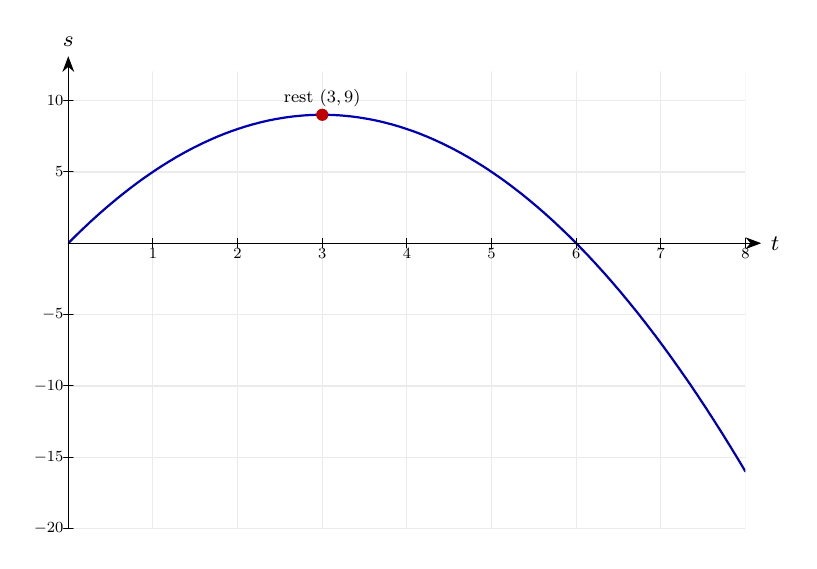
\begin{tikzpicture}[>={Stealth[length=2mm]},font=\footnotesize,line cap=round,line join=round]
\begin{scope}
\clip (0,0) rectangle (8.6,5.8);
\draw[gray!16] (0,0) grid[xstep=1.075,ystep=0.906] (8.6,5.8);
\draw[blue!70!black,thick] (0,3.625) -- (0.031,3.656) -- (0.061,3.687) -- (0.092,3.717) -- (0.123,3.747) -- (0.154,3.777) -- (0.184,3.806) -- (0.215,3.835) -- (0.246,3.864) -- (0.276,3.893) -- (0.307,3.921) -- (0.338,3.949) -- (0.369,3.977) -- (0.399,4.004) -- (0.43,4.031) -- (0.461,4.058) -- (0.491,4.084) -- (0.522,4.11) -- (0.553,4.136) -- (0.584,4.162) -- (0.614,4.187) -- (0.645,4.212) -- (0.676,4.237) -- (0.706,4.261) -- (0.737,4.285) -- (0.768,4.309) -- (0.799,4.333) -- (0.829,4.356) -- (0.86,4.379) -- (0.891,4.402) -- (0.921,4.424) -- (0.952,4.446) -- (0.983,4.468) -- (1.014,4.489) -- (1.044,4.51) -- (1.075,4.531) -- (1.106,4.552) -- (1.136,4.572) -- (1.167,4.592) -- (1.198,4.612) -- (1.229,4.631) -- (1.259,4.65) -- (1.29,4.669) -- (1.321,4.687) -- (1.351,4.706) -- (1.382,4.724) -- (1.413,4.741) -- (1.444,4.759) -- (1.474,4.776) -- (1.505,4.792) -- (1.536,4.809) -- (1.566,4.825) -- (1.597,4.841) -- (1.628,4.856) -- (1.659,4.871) -- (1.689,4.886) -- (1.72,4.901) -- (1.751,4.915) -- (1.781,4.929) -- (1.812,4.943) -- (1.843,4.957) -- (1.874,4.97) -- (1.904,4.983) -- (1.935,4.995) -- (1.966,5.008) -- (1.996,5.02) -- (2.027,5.031) -- (2.058,5.043) -- (2.089,5.054) -- (2.119,5.064) -- (2.15,5.075) -- (2.181,5.085) -- (2.211,5.095) -- (2.242,5.105) -- (2.273,5.114) -- (2.304,5.123) -- (2.334,5.132) -- (2.365,5.14) -- (2.396,5.148) -- (2.426,5.156) -- (2.457,5.164) -- (2.488,5.171) -- (2.519,5.178) -- (2.549,5.185) -- (2.58,5.191) -- (2.611,5.197) -- (2.641,5.203) -- (2.672,5.208) -- (2.703,5.213) -- (2.734,5.218) -- (2.764,5.223) -- (2.795,5.227) -- (2.826,5.231) -- (2.856,5.235) -- (2.887,5.238) -- (2.918,5.241) -- (2.949,5.244) -- (2.979,5.247) -- (3.01,5.249) -- (3.041,5.251) -- (3.071,5.253) -- (3.102,5.254) -- (3.133,5.255) -- (3.164,5.256) -- (3.194,5.256) -- (3.225,5.256) -- (3.256,5.256) -- (3.286,5.256) -- (3.317,5.255) -- (3.348,5.254) -- (3.379,5.253) -- (3.409,5.251) -- (3.44,5.249) -- (3.471,5.247) -- (3.501,5.244) -- (3.532,5.241) -- (3.563,5.238) -- (3.594,5.235) -- (3.624,5.231) -- (3.655,5.227) -- (3.686,5.223) -- (3.716,5.218) -- (3.747,5.213) -- (3.778,5.208) -- (3.809,5.203) -- (3.839,5.197) -- (3.87,5.191) -- (3.901,5.185) -- (3.931,5.178) -- (3.962,5.171) -- (3.993,5.164) -- (4.024,5.156) -- (4.054,5.148) -- (4.085,5.14) -- (4.116,5.132) -- (4.146,5.123) -- (4.177,5.114) -- (4.208,5.105) -- (4.239,5.095) -- (4.269,5.085) -- (4.3,5.075) -- (4.331,5.064) -- (4.361,5.054) -- (4.392,5.043) -- (4.423,5.031) -- (4.454,5.02) -- (4.484,5.008) -- (4.515,4.995) -- (4.546,4.983) -- (4.576,4.97) -- (4.607,4.957) -- (4.638,4.943) -- (4.669,4.929) -- (4.699,4.915) -- (4.73,4.901) -- (4.761,4.886) -- (4.791,4.871) -- (4.822,4.856) -- (4.853,4.841) -- (4.884,4.825) -- (4.914,4.809) -- (4.945,4.792) -- (4.976,4.776) -- (5.006,4.759) -- (5.037,4.741) -- (5.068,4.724) -- (5.099,4.706) -- (5.129,4.687) -- (5.16,4.669) -- (5.191,4.65) -- (5.221,4.631) -- (5.252,4.612) -- (5.283,4.592) -- (5.314,4.572) -- (5.344,4.552) -- (5.375,4.531) -- (5.406,4.51) -- (5.436,4.489) -- (5.467,4.468) -- (5.498,4.446) -- (5.529,4.424) -- (5.559,4.402) -- (5.59,4.379) -- (5.621,4.356) -- (5.651,4.333) -- (5.682,4.309) -- (5.713,4.285) -- (5.744,4.261) -- (5.774,4.237) -- (5.805,4.212) -- (5.836,4.187) -- (5.866,4.162) -- (5.897,4.136) -- (5.928,4.11) -- (5.959,4.084) -- (5.989,4.058) -- (6.02,4.031) -- (6.051,4.004) -- (6.081,3.977) -- (6.112,3.949) -- (6.143,3.921) -- (6.174,3.893) -- (6.204,3.864) -- (6.235,3.835) -- (6.266,3.806) -- (6.296,3.777) -- (6.327,3.747) -- (6.358,3.717) -- (6.389,3.687) -- (6.419,3.656) -- (6.45,3.625) -- (6.481,3.594) -- (6.511,3.562) -- (6.542,3.53) -- (6.573,3.498) -- (6.604,3.466) -- (6.634,3.433) -- (6.665,3.4) -- (6.696,3.367) -- (6.726,3.333) -- (6.757,3.299) -- (6.788,3.265) -- (6.819,3.231) -- (6.849,3.196) -- (6.88,3.161) -- (6.911,3.126) -- (6.941,3.09) -- (6.972,3.054) -- (7.003,3.018) -- (7.034,2.981) -- (7.064,2.944) -- (7.095,2.907) -- (7.126,2.87) -- (7.156,2.832) -- (7.187,2.794) -- (7.218,2.756) -- (7.249,2.717) -- (7.279,2.678) -- (7.31,2.639) -- (7.341,2.599) -- (7.371,2.56) -- (7.402,2.52) -- (7.433,2.479) -- (7.464,2.439) -- (7.494,2.398) -- (7.525,2.356) -- (7.556,2.315) -- (7.586,2.273) -- (7.617,2.231) -- (7.648,2.188) -- (7.679,2.145) -- (7.709,2.102) -- (7.74,2.059) -- (7.771,2.015) -- (7.801,1.971) -- (7.832,1.927) -- (7.863,1.883) -- (7.894,1.838) -- (7.924,1.793) -- (7.955,1.747) -- (7.986,1.702) -- (8.016,1.656) -- (8.047,1.609) -- (8.078,1.563) -- (8.109,1.516) -- (8.139,1.468) -- (8.17,1.421) -- (8.201,1.373) -- (8.231,1.325) -- (8.262,1.277) -- (8.293,1.228) -- (8.324,1.179) -- (8.354,1.13) -- (8.385,1.08) -- (8.416,1.03) -- (8.446,0.98) -- (8.477,0.93) -- (8.508,0.879) -- (8.539,0.828) -- (8.569,0.777) -- (8.6,0.725);
\end{scope}
\draw[->] (0,3.625) -- (8.8,3.625) node[right]{$t$};
\draw[->] (0,0) -- (0,6) node[above]{$s$};
\draw (1.075,3.565) -- (1.075,3.685) node[below=1pt,scale=0.7]{$1$};
\draw (2.15,3.565) -- (2.15,3.685) node[below=1pt,scale=0.7]{$2$};
\draw (3.225,3.565) -- (3.225,3.685) node[below=1pt,scale=0.7]{$3$};
\draw (4.3,3.565) -- (4.3,3.685) node[below=1pt,scale=0.7]{$4$};
\draw (5.375,3.565) -- (5.375,3.685) node[below=1pt,scale=0.7]{$5$};
\draw (6.45,3.565) -- (6.45,3.685) node[below=1pt,scale=0.7]{$6$};
\draw (7.525,3.565) -- (7.525,3.685) node[below=1pt,scale=0.7]{$7$};
\draw (8.6,3.565) -- (8.6,3.685) node[below=1pt,scale=0.7]{$8$};
\draw (-0.06,0) -- (0.06,0) node[left=1pt,scale=0.7]{$-20$};
\draw (-0.06,0.906) -- (0.06,0.906) node[left=1pt,scale=0.7]{$-15$};
\draw (-0.06,1.813) -- (0.06,1.813) node[left=1pt,scale=0.7]{$-10$};
\draw (-0.06,2.719) -- (0.06,2.719) node[left=1pt,scale=0.7]{$-5$};
\draw (-0.06,4.531) -- (0.06,4.531) node[left=1pt,scale=0.7]{$5$};
\draw (-0.06,5.438) -- (0.06,5.438) node[left=1pt,scale=0.7]{$10$};
\fill[red!75!black] (3.225,5.256) circle (2.2pt);
\node[above,scale=0.78] at (3.225,5.256) {rest $(3,9)$};
\end{tikzpicture}
}
\end{center}
\small The model plotted against its variable, with the key point(s) marked.\normalsize

\medskip\hrule

\section*{Real-Life Problems 27\quad\small\texttt{(d5-027)}}
\addcontentsline{toc}{section}{Real-Life Problems 27 (d5-027)}
\textit{Difficulty: Foundation \quad\textbar\quad Marks: 7}

\question{An open-topped cylindrical bucket is to be made from a fixed area of metal \( 300\pi \) cm\(^2\). The radius is \( r \) cm and the height is \( h \) cm. (a) Show that \( h = \dfrac{300 - r^2}{2r} \). (b) Show that the volume is \( V = \dfrac{\pi r}{2}(300 - r^2) \). (c) Find the value of \( r \) that maximises the volume.}

\textbf{Worked solution.}

\textit{Step 1: (a) Surface area (open top): base + curved side.}
\[\begin{gathered}
\pi r^2 + 2\pi r h = 300\pi \implies r^2 + 2rh = 300 \implies h = \frac{300 - r^2}{2r}
\end{gathered}\]
Rearrange to make \( h \) the subject.

\textit{Step 2: (b) Volume.}
\[\begin{gathered}
V = \pi r^2 h = \pi r^2 \cdot \frac{300 - r^2}{2r} = \frac{\pi r(300 - r^2)}{2}
\end{gathered}\]
Substitute \( h \) into \( V = \pi r^2 h \) and simplify.

\textit{Step 3: (c) Expand and differentiate.}
\[\begin{gathered}
V = \frac{\pi}{2}(300r - r^3) \implies \frac{\mathrm{d}V}{\mathrm{d}r} = \frac{\pi}{2}(300 - 3r^2)
\end{gathered}\]
Power rule applied inside the bracket.

\textit{Step 4: Set to zero.}
\[\begin{gathered}
300 - 3r^2 = 0 \implies r^2 = 100 \implies r = 10 \text{ cm}
\end{gathered}\]
Take the positive root.

\textit{Step 5: Confirm maximum.}
\[\begin{gathered}
\frac{\mathrm{d}^2V}{\mathrm{d}r^2} = \frac{\pi}{2}(-6r); \quad r=10: -30\pi < 0 \Rightarrow \text{maximum}
\end{gathered}\]
Negative second derivative.

\begin{answerbox}
\textbf{Final answer:}\quad (a) Shown. \\[3pt]  (b) Shown. \\[3pt]  (c) \(\displaystyle  r = 10 \) cm
\end{answerbox}
\textbf{Diagram.}

\begin{center}
\resizebox{\ifdim\width>\linewidth \linewidth\else \width\fi}{!}{%
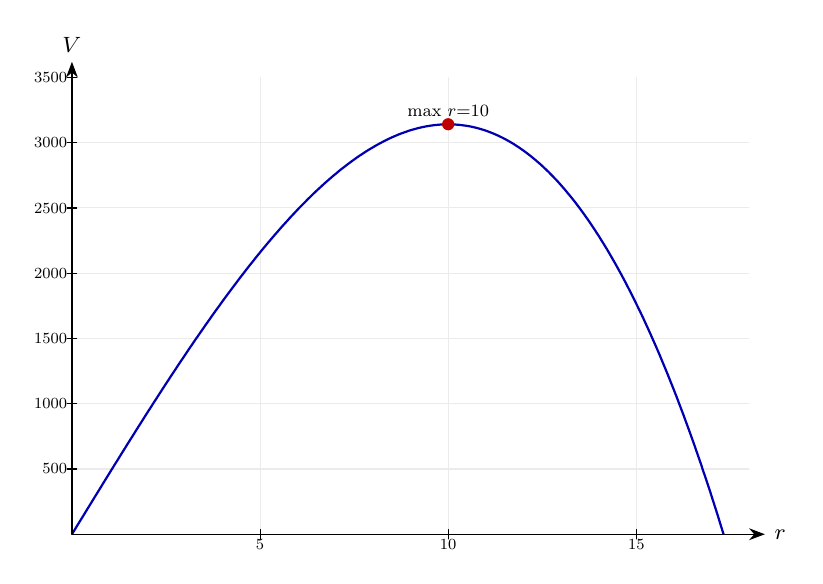
\begin{tikzpicture}[>={Stealth[length=2mm]},font=\footnotesize,line cap=round,line join=round]
\begin{scope}
\clip (0,0) rectangle (8.6,5.8);
\draw[gray!16] (0,0) grid[xstep=2.389,ystep=0.829] (8.6,5.8);
\draw[blue!70!black,thick] (0,0) -- (0.031,0.05) -- (0.061,0.1) -- (0.092,0.151) -- (0.123,0.201) -- (0.154,0.251) -- (0.184,0.301) -- (0.215,0.351) -- (0.246,0.401) -- (0.276,0.451) -- (0.307,0.501) -- (0.338,0.551) -- (0.369,0.601) -- (0.399,0.651) -- (0.43,0.701) -- (0.461,0.751) -- (0.491,0.8) -- (0.522,0.85) -- (0.553,0.9) -- (0.584,0.949) -- (0.614,0.998) -- (0.645,1.048) -- (0.676,1.097) -- (0.706,1.146) -- (0.737,1.195) -- (0.768,1.244) -- (0.799,1.293) -- (0.829,1.342) -- (0.86,1.39) -- (0.891,1.439) -- (0.921,1.487) -- (0.952,1.536) -- (0.983,1.584) -- (1.014,1.632) -- (1.044,1.68) -- (1.075,1.727) -- (1.106,1.775) -- (1.136,1.822) -- (1.167,1.87) -- (1.198,1.917) -- (1.229,1.964) -- (1.259,2.011) -- (1.29,2.057) -- (1.321,2.104) -- (1.351,2.15) -- (1.382,2.196) -- (1.413,2.242) -- (1.444,2.288) -- (1.474,2.333) -- (1.505,2.379) -- (1.536,2.424) -- (1.566,2.469) -- (1.597,2.513) -- (1.628,2.558) -- (1.659,2.602) -- (1.689,2.646) -- (1.72,2.69) -- (1.751,2.733) -- (1.781,2.777) -- (1.812,2.82) -- (1.843,2.863) -- (1.874,2.905) -- (1.904,2.948) -- (1.935,2.99) -- (1.966,3.032) -- (1.996,3.073) -- (2.027,3.114) -- (2.058,3.155) -- (2.089,3.196) -- (2.119,3.237) -- (2.15,3.277) -- (2.181,3.317) -- (2.211,3.356) -- (2.242,3.396) -- (2.273,3.435) -- (2.304,3.473) -- (2.334,3.512) -- (2.365,3.55) -- (2.396,3.588) -- (2.426,3.625) -- (2.457,3.662) -- (2.488,3.699) -- (2.519,3.735) -- (2.549,3.771) -- (2.58,3.807) -- (2.611,3.842) -- (2.641,3.877) -- (2.672,3.912) -- (2.703,3.946) -- (2.734,3.98) -- (2.764,4.014) -- (2.795,4.047) -- (2.826,4.08) -- (2.856,4.112) -- (2.887,4.145) -- (2.918,4.176) -- (2.949,4.207) -- (2.979,4.238) -- (3.01,4.269) -- (3.041,4.299) -- (3.071,4.329) -- (3.102,4.358) -- (3.133,4.387) -- (3.164,4.415) -- (3.194,4.443) -- (3.225,4.471) -- (3.256,4.498) -- (3.286,4.524) -- (3.317,4.551) -- (3.348,4.576) -- (3.379,4.602) -- (3.409,4.627) -- (3.44,4.651) -- (3.471,4.675) -- (3.501,4.698) -- (3.532,4.721) -- (3.563,4.744) -- (3.594,4.766) -- (3.624,4.788) -- (3.655,4.809) -- (3.686,4.829) -- (3.716,4.849) -- (3.747,4.869) -- (3.778,4.888) -- (3.809,4.906) -- (3.839,4.924) -- (3.87,4.942) -- (3.901,4.959) -- (3.931,4.975) -- (3.962,4.991) -- (3.993,5.007) -- (4.024,5.022) -- (4.054,5.036) -- (4.085,5.05) -- (4.116,5.063) -- (4.146,5.076) -- (4.177,5.088) -- (4.208,5.099) -- (4.239,5.11) -- (4.269,5.121) -- (4.3,5.131) -- (4.331,5.14) -- (4.361,5.148) -- (4.392,5.157) -- (4.423,5.164) -- (4.454,5.171) -- (4.484,5.177) -- (4.515,5.183) -- (4.546,5.188) -- (4.576,5.192) -- (4.607,5.196) -- (4.638,5.199) -- (4.669,5.202) -- (4.699,5.204) -- (4.73,5.205) -- (4.761,5.206) -- (4.791,5.206) -- (4.822,5.205) -- (4.853,5.204) -- (4.884,5.202) -- (4.914,5.2) -- (4.945,5.196) -- (4.976,5.192) -- (5.006,5.188) -- (5.037,5.183) -- (5.068,5.177) -- (5.099,5.17) -- (5.129,5.163) -- (5.16,5.155) -- (5.191,5.146) -- (5.221,5.137) -- (5.252,5.127) -- (5.283,5.116) -- (5.314,5.104) -- (5.344,5.092) -- (5.375,5.079) -- (5.406,5.065) -- (5.436,5.051) -- (5.467,5.036) -- (5.498,5.02) -- (5.529,5.003) -- (5.559,4.986) -- (5.59,4.968) -- (5.621,4.949) -- (5.651,4.929) -- (5.682,4.909) -- (5.713,4.887) -- (5.744,4.865) -- (5.774,4.843) -- (5.805,4.819) -- (5.836,4.795) -- (5.866,4.77) -- (5.897,4.744) -- (5.928,4.717) -- (5.959,4.69) -- (5.989,4.662) -- (6.02,4.632) -- (6.051,4.603) -- (6.081,4.572) -- (6.112,4.54) -- (6.143,4.508) -- (6.174,4.475) -- (6.204,4.441) -- (6.235,4.406) -- (6.266,4.37) -- (6.296,4.333) -- (6.327,4.296) -- (6.358,4.258) -- (6.389,4.219) -- (6.419,4.179) -- (6.45,4.138) -- (6.481,4.096) -- (6.511,4.054) -- (6.542,4.01) -- (6.573,3.966) -- (6.604,3.92) -- (6.634,3.874) -- (6.665,3.827) -- (6.696,3.779) -- (6.726,3.73) -- (6.757,3.681) -- (6.788,3.63) -- (6.819,3.578) -- (6.849,3.526) -- (6.88,3.472) -- (6.911,3.418) -- (6.941,3.363) -- (6.972,3.307) -- (7.003,3.249) -- (7.034,3.191) -- (7.064,3.132) -- (7.095,3.072) -- (7.126,3.011) -- (7.156,2.949) -- (7.187,2.886) -- (7.218,2.822) -- (7.249,2.758) -- (7.279,2.692) -- (7.31,2.625) -- (7.341,2.557) -- (7.371,2.488) -- (7.402,2.419) -- (7.433,2.348) -- (7.464,2.276) -- (7.494,2.203) -- (7.525,2.129) -- (7.556,2.054) -- (7.586,1.979) -- (7.617,1.902) -- (7.648,1.824) -- (7.679,1.745) -- (7.709,1.665) -- (7.74,1.584) -- (7.771,1.502) -- (7.801,1.419) -- (7.832,1.335) -- (7.863,1.249) -- (7.894,1.163) -- (7.924,1.076) -- (7.955,0.987) -- (7.986,0.898) -- (8.016,0.807) -- (8.047,0.715) -- (8.078,0.623) -- (8.109,0.529) -- (8.139,0.434) -- (8.17,0.338) -- (8.201,0.241) -- (8.231,0.142) -- (8.262,0.043) -- (8.293,-0.057) -- (8.324,-0.159) -- (8.354,-0.262) -- (8.385,-0.366) -- (8.416,-0.471) -- (8.446,-0.577) -- (8.477,-0.684) -- (8.508,-0.792) -- (8.539,-0.902) -- (8.569,-1.013) -- (8.6,-1.125);
\end{scope}
\draw[->] (0,0) -- (8.8,0) node[right]{$r$};
\draw[->] (0,0) -- (0,6) node[above]{$V$};
\draw (2.389,-0.06) -- (2.389,0.06) node[below=1pt,scale=0.7]{$5$};
\draw (4.778,-0.06) -- (4.778,0.06) node[below=1pt,scale=0.7]{$10$};
\draw (7.167,-0.06) -- (7.167,0.06) node[below=1pt,scale=0.7]{$15$};
\draw (-0.06,0.829) -- (0.06,0.829) node[left=1pt,scale=0.7]{$500$};
\draw (-0.06,1.657) -- (0.06,1.657) node[left=1pt,scale=0.7]{$1000$};
\draw (-0.06,2.486) -- (0.06,2.486) node[left=1pt,scale=0.7]{$1500$};
\draw (-0.06,3.314) -- (0.06,3.314) node[left=1pt,scale=0.7]{$2000$};
\draw (-0.06,4.143) -- (0.06,4.143) node[left=1pt,scale=0.7]{$2500$};
\draw (-0.06,4.971) -- (0.06,4.971) node[left=1pt,scale=0.7]{$3000$};
\draw (-0.06,5.8) -- (0.06,5.8) node[left=1pt,scale=0.7]{$3500$};
\fill[red!75!black] (4.778,5.207) circle (2.2pt);
\node[above,scale=0.78] at (4.778,5.207) {max $r{=}10$};
\end{tikzpicture}
}
\end{center}
\small The model plotted against its variable, with the key point(s) marked.\normalsize

\medskip\hrule

\section*{Real-Life Problems 28\quad\small\texttt{(d5-028)}}
\addcontentsline{toc}{section}{Real-Life Problems 28 (d5-028)}
\textit{Difficulty: Foundation \quad\textbar\quad Marks: 6}

\question{A particle moves along the \( x \)-axis. Its displacement is \( x = t^3 - 6t^2 + 12t - 3 \) metres at time \( t \) seconds. (a) Find the velocity and acceleration functions. (b) Find the time when the acceleration is zero. (c) Show that the velocity is always positive for \( t \geq 0 \).}

\textbf{Worked solution.}

\textit{Step 1: (a) Velocity.}
\[\begin{gathered}
v = \frac{\mathrm{d}x}{\mathrm{d}t} = 3t^2 - 12t + 12
\end{gathered}\]
Power rule.

\textit{Step 2: Acceleration.}
\[\begin{gathered}
a = \frac{\mathrm{d}v}{\mathrm{d}t} = 6t - 12
\end{gathered}\]
Differentiate \( v \).

\textit{Step 3: (b) Set \( a = 0 \).}
\[\begin{gathered}
6t - 12 = 0 \implies t = 2 \text{ s}
\end{gathered}\]
Solve the linear equation.

\textit{Step 4: (c) Factorise or complete the square for \( v \).}
\[\begin{gathered}
v = 3t^2 - 12t + 12 = 3(t^2 - 4t + 4) = 3(t - 2)^2
\end{gathered}\]
Recognise the perfect square.

\textit{Step 5: Conclude.}
\[\begin{gathered}
v = 3(t-2)^2 \geq 0 \text{ for all } t
\end{gathered}\]
A square is always \( \geq 0 \), so velocity is never negative. At \( t = 2 \) it equals zero momentarily, but is positive otherwise.

\begin{answerbox}
\textbf{Final answer:}\quad (a) \(\displaystyle  v = 3t^2-12t+12 \), \(\displaystyle  a = 6t-12 \) \\[3pt]  (b) \(\displaystyle  t = 2 \) s \\[3pt]  (c) \(\displaystyle  v = 3(t-2)^2 \geq 0 \) for all \(\displaystyle  t \geq 0 \) $\checkmark$
\end{answerbox}
\textbf{Diagram.}

\begin{center}
\resizebox{\ifdim\width>\linewidth \linewidth\else \width\fi}{!}{%
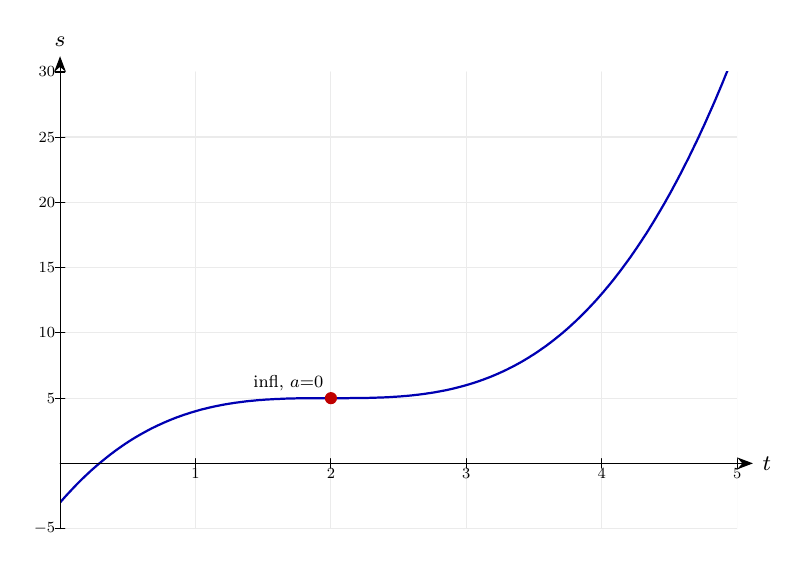
\begin{tikzpicture}[>={Stealth[length=2mm]},font=\footnotesize,line cap=round,line join=round]
\begin{scope}
\clip (0,0) rectangle (8.6,5.8);
\draw[gray!16] (0,0) grid[xstep=1.72,ystep=0.829] (8.6,5.8);
\draw[blue!70!black,thick] (0,0.331) -- (0.031,0.367) -- (0.061,0.401) -- (0.092,0.435) -- (0.123,0.468) -- (0.154,0.501) -- (0.184,0.533) -- (0.215,0.565) -- (0.246,0.596) -- (0.276,0.626) -- (0.307,0.656) -- (0.338,0.685) -- (0.369,0.714) -- (0.399,0.742) -- (0.43,0.769) -- (0.461,0.796) -- (0.491,0.822) -- (0.522,0.848) -- (0.553,0.873) -- (0.584,0.898) -- (0.614,0.922) -- (0.645,0.946) -- (0.676,0.969) -- (0.706,0.992) -- (0.737,1.014) -- (0.768,1.036) -- (0.799,1.057) -- (0.829,1.078) -- (0.86,1.098) -- (0.891,1.118) -- (0.921,1.137) -- (0.952,1.156) -- (0.983,1.174) -- (1.014,1.192) -- (1.044,1.209) -- (1.075,1.226) -- (1.106,1.243) -- (1.136,1.259) -- (1.167,1.275) -- (1.198,1.29) -- (1.229,1.305) -- (1.259,1.319) -- (1.29,1.333) -- (1.321,1.347) -- (1.351,1.36) -- (1.382,1.373) -- (1.413,1.386) -- (1.444,1.398) -- (1.474,1.41) -- (1.505,1.421) -- (1.536,1.432) -- (1.566,1.443) -- (1.597,1.453) -- (1.628,1.463) -- (1.659,1.473) -- (1.689,1.482) -- (1.72,1.491) -- (1.751,1.5) -- (1.781,1.509) -- (1.812,1.517) -- (1.843,1.524) -- (1.874,1.532) -- (1.904,1.539) -- (1.935,1.546) -- (1.966,1.553) -- (1.996,1.559) -- (2.027,1.565) -- (2.058,1.571) -- (2.089,1.577) -- (2.119,1.582) -- (2.15,1.587) -- (2.181,1.592) -- (2.211,1.597) -- (2.242,1.601) -- (2.273,1.605) -- (2.304,1.609) -- (2.334,1.613) -- (2.365,1.617) -- (2.396,1.62) -- (2.426,1.623) -- (2.457,1.626) -- (2.488,1.629) -- (2.519,1.632) -- (2.549,1.634) -- (2.58,1.636) -- (2.611,1.639) -- (2.641,1.641) -- (2.672,1.642) -- (2.703,1.644) -- (2.734,1.646) -- (2.764,1.647) -- (2.795,1.648) -- (2.826,1.65) -- (2.856,1.651) -- (2.887,1.652) -- (2.918,1.653) -- (2.949,1.653) -- (2.979,1.654) -- (3.01,1.655) -- (3.041,1.655) -- (3.071,1.656) -- (3.102,1.656) -- (3.133,1.656) -- (3.164,1.656) -- (3.194,1.657) -- (3.225,1.657) -- (3.256,1.657) -- (3.286,1.657) -- (3.317,1.657) -- (3.348,1.657) -- (3.379,1.657) -- (3.409,1.657) -- (3.44,1.657) -- (3.471,1.657) -- (3.501,1.657) -- (3.532,1.657) -- (3.563,1.657) -- (3.594,1.657) -- (3.624,1.657) -- (3.655,1.657) -- (3.686,1.658) -- (3.716,1.658) -- (3.747,1.658) -- (3.778,1.658) -- (3.809,1.659) -- (3.839,1.659) -- (3.87,1.66) -- (3.901,1.66) -- (3.931,1.661) -- (3.962,1.662) -- (3.993,1.663) -- (4.024,1.664) -- (4.054,1.665) -- (4.085,1.666) -- (4.116,1.667) -- (4.146,1.669) -- (4.177,1.67) -- (4.208,1.672) -- (4.239,1.674) -- (4.269,1.676) -- (4.3,1.678) -- (4.331,1.68) -- (4.361,1.683) -- (4.392,1.685) -- (4.423,1.688) -- (4.454,1.691) -- (4.484,1.694) -- (4.515,1.698) -- (4.546,1.701) -- (4.576,1.705) -- (4.607,1.709) -- (4.638,1.713) -- (4.669,1.718) -- (4.699,1.722) -- (4.73,1.727) -- (4.761,1.732) -- (4.791,1.738) -- (4.822,1.743) -- (4.853,1.749) -- (4.884,1.755) -- (4.914,1.761) -- (4.945,1.768) -- (4.976,1.775) -- (5.006,1.782) -- (5.037,1.79) -- (5.068,1.798) -- (5.099,1.806) -- (5.129,1.814) -- (5.16,1.823) -- (5.191,1.832) -- (5.221,1.841) -- (5.252,1.851) -- (5.283,1.861) -- (5.314,1.871) -- (5.344,1.882) -- (5.375,1.893) -- (5.406,1.905) -- (5.436,1.916) -- (5.467,1.928) -- (5.498,1.941) -- (5.529,1.954) -- (5.559,1.967) -- (5.59,1.981) -- (5.621,1.995) -- (5.651,2.009) -- (5.682,2.024) -- (5.713,2.04) -- (5.744,2.055) -- (5.774,2.071) -- (5.805,2.088) -- (5.836,2.105) -- (5.866,2.122) -- (5.897,2.14) -- (5.928,2.159) -- (5.959,2.177) -- (5.989,2.197) -- (6.02,2.216) -- (6.051,2.237) -- (6.081,2.257) -- (6.112,2.279) -- (6.143,2.3) -- (6.174,2.322) -- (6.204,2.345) -- (6.235,2.368) -- (6.266,2.392) -- (6.296,2.416) -- (6.327,2.441) -- (6.358,2.466) -- (6.389,2.492) -- (6.419,2.518) -- (6.45,2.545) -- (6.481,2.573) -- (6.511,2.601) -- (6.542,2.629) -- (6.573,2.659) -- (6.604,2.688) -- (6.634,2.719) -- (6.665,2.749) -- (6.696,2.781) -- (6.726,2.813) -- (6.757,2.846) -- (6.788,2.879) -- (6.819,2.913) -- (6.849,2.948) -- (6.88,2.983) -- (6.911,3.019) -- (6.941,3.055) -- (6.972,3.092) -- (7.003,3.13) -- (7.034,3.168) -- (7.064,3.208) -- (7.095,3.247) -- (7.126,3.288) -- (7.156,3.329) -- (7.187,3.371) -- (7.218,3.413) -- (7.249,3.456) -- (7.279,3.5) -- (7.31,3.545) -- (7.341,3.59) -- (7.371,3.636) -- (7.402,3.683) -- (7.433,3.73) -- (7.464,3.778) -- (7.494,3.827) -- (7.525,3.877) -- (7.556,3.928) -- (7.586,3.979) -- (7.617,4.031) -- (7.648,4.084) -- (7.679,4.137) -- (7.709,4.191) -- (7.74,4.246) -- (7.771,4.302) -- (7.801,4.359) -- (7.832,4.416) -- (7.863,4.475) -- (7.894,4.534) -- (7.924,4.594) -- (7.955,4.655) -- (7.986,4.716) -- (8.016,4.779) -- (8.047,4.842) -- (8.078,4.906) -- (8.109,4.971) -- (8.139,5.037) -- (8.17,5.103) -- (8.201,5.171) -- (8.231,5.24) -- (8.262,5.309) -- (8.293,5.379) -- (8.324,5.45) -- (8.354,5.522) -- (8.385,5.595) -- (8.416,5.669) -- (8.446,5.744) -- (8.477,5.819) -- (8.508,5.896) -- (8.539,5.974) -- (8.569,6.052) -- (8.6,6.131);
\end{scope}
\draw[->] (0,0.829) -- (8.8,0.829) node[right]{$t$};
\draw[->] (0,0) -- (0,6) node[above]{$s$};
\draw (1.72,0.769) -- (1.72,0.889) node[below=1pt,scale=0.7]{$1$};
\draw (3.44,0.769) -- (3.44,0.889) node[below=1pt,scale=0.7]{$2$};
\draw (5.16,0.769) -- (5.16,0.889) node[below=1pt,scale=0.7]{$3$};
\draw (6.88,0.769) -- (6.88,0.889) node[below=1pt,scale=0.7]{$4$};
\draw (8.6,0.769) -- (8.6,0.889) node[below=1pt,scale=0.7]{$5$};
\draw (-0.06,0) -- (0.06,0) node[left=1pt,scale=0.7]{$-5$};
\draw (-0.06,1.657) -- (0.06,1.657) node[left=1pt,scale=0.7]{$5$};
\draw (-0.06,2.486) -- (0.06,2.486) node[left=1pt,scale=0.7]{$10$};
\draw (-0.06,3.314) -- (0.06,3.314) node[left=1pt,scale=0.7]{$15$};
\draw (-0.06,4.143) -- (0.06,4.143) node[left=1pt,scale=0.7]{$20$};
\draw (-0.06,4.971) -- (0.06,4.971) node[left=1pt,scale=0.7]{$25$};
\draw (-0.06,5.8) -- (0.06,5.8) node[left=1pt,scale=0.7]{$30$};
\fill[red!75!black] (3.44,1.657) circle (2.2pt);
\node[above left,scale=0.78] at (3.44,1.657) {infl, $a{=}0$};
\end{tikzpicture}
}
\end{center}
\small The model plotted against its variable, with the key point(s) marked.\normalsize

\medskip\hrule

\section*{Real-Life Problems 29\quad\small\texttt{(d5-029)}}
\addcontentsline{toc}{section}{Real-Life Problems 29 (d5-029)}
\textit{Difficulty: Foundation \quad\textbar\quad Marks: 6}

\question{A farmer needs to fence a rectangular area of \( 200 \) m\(^2\) on all four sides. (a) Let the width be \( x \) m. Write down the length in terms of \( x \). (b) Find an expression for the total length of fencing needed. (c) Use calculus to find the dimensions that minimise the fencing used.}

\textbf{Worked solution.}

\textit{Step 1: (a) Area = \( x \times l = 200 \).}
\[\begin{gathered}
l = \frac{200}{x}
\end{gathered}\]
Rearrange the area formula.

\textit{Step 2: (b) Total fencing.}
\[\begin{gathered}
P = 2x + 2l = 2x + \frac{400}{x}
\end{gathered}\]
Substitute \( l = \dfrac{200}{x} \) into the perimeter formula.

\textit{Step 3: (c) Differentiate.}
\[\begin{gathered}
\frac{\mathrm{d}P}{\mathrm{d}x} = 2 - \frac{400}{x^2}
\end{gathered}\]
\( \dfrac{\mathrm{d}}{\mathrm{d}x}\left(\dfrac{400}{x}\right) = -\dfrac{400}{x^2} \).

\textit{Step 4: Set to zero.}
\[\begin{gathered}
2 = \frac{400}{x^2} \implies x^2 = 200 \implies x = 10\sqrt{2} \approx 14.1 \text{ m}
\end{gathered}\]
Solve for \( x \).

\textit{Step 5: Confirm minimum and find length.}
\[\begin{gathered}
\frac{\mathrm{d}^2P}{\mathrm{d}x^2} = \frac{800}{x^3} > 0 \Rightarrow \text{minimum}; \quad l = \frac{200}{10\sqrt{2}} = 10\sqrt{2}
\end{gathered}\]
The optimal shape is again a square.

\begin{answerbox}
\textbf{Final answer:}\quad (a) \(\displaystyle  l = \dfrac{200}{x} \) \\[3pt]  (b) \(\displaystyle  P = 2x + \dfrac{400}{x} \) \\[3pt]  (c) Both dimensions \(\displaystyle  = 10\sqrt{2} \approx 14.1 \) m; minimum fencing \(\displaystyle  = 40\sqrt{2} \approx 56.6 \) m
\end{answerbox}
\textbf{Diagram.}

\begin{center}
\resizebox{\ifdim\width>\linewidth \linewidth\else \width\fi}{!}{%
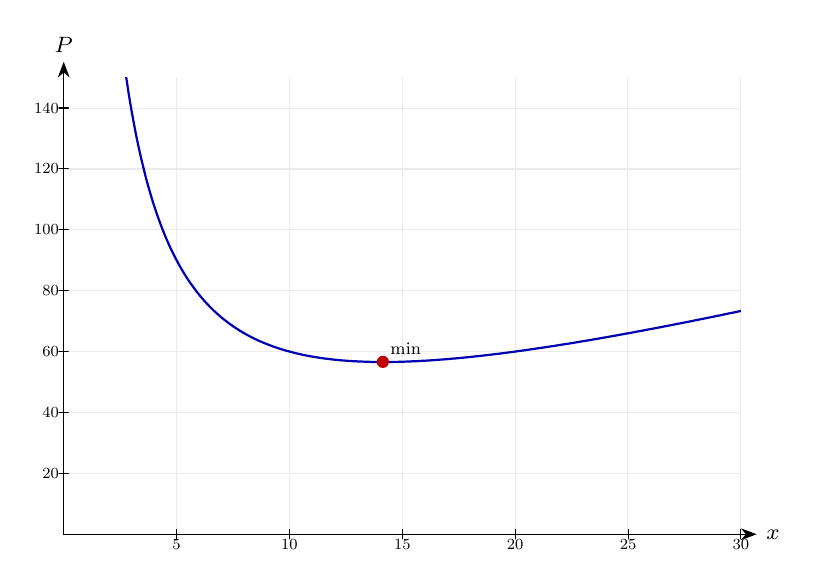
\begin{tikzpicture}[>={Stealth[length=2mm]},font=\footnotesize,line cap=round,line join=round]
\begin{scope}
\clip (0,0) rectangle (8.6,5.8);
\draw[gray!16] (0,0) grid[xstep=1.433,ystep=0.773] (8.6,5.8);
\draw[blue!70!black,thick] (0.031,11.6) -- (0.061,11.6) -- (0.092,11.6) -- (0.123,11.6) -- (0.154,11.6) -- (0.184,11.6) -- (0.215,11.6) -- (0.246,11.6) -- (0.276,11.6) -- (0.307,11.6) -- (0.338,11.6) -- (0.369,11.6) -- (0.399,11.212) -- (0.43,10.427) -- (0.461,9.748) -- (0.491,9.155) -- (0.522,8.632) -- (0.553,8.169) -- (0.584,7.755) -- (0.614,7.383) -- (0.645,7.048) -- (0.676,6.744) -- (0.706,6.467) -- (0.737,6.214) -- (0.768,5.981) -- (0.799,5.768) -- (0.829,5.57) -- (0.86,5.388) -- (0.891,5.218) -- (0.921,5.06) -- (0.952,4.913) -- (0.983,4.776) -- (1.014,4.648) -- (1.044,4.527) -- (1.075,4.414) -- (1.106,4.308) -- (1.136,4.208) -- (1.167,4.114) -- (1.198,4.025) -- (1.229,3.94) -- (1.259,3.861) -- (1.29,3.785) -- (1.321,3.713) -- (1.351,3.645) -- (1.382,3.581) -- (1.413,3.519) -- (1.444,3.461) -- (1.474,3.405) -- (1.505,3.352) -- (1.536,3.301) -- (1.566,3.253) -- (1.597,3.207) -- (1.628,3.163) -- (1.659,3.121) -- (1.689,3.08) -- (1.72,3.042) -- (1.751,3.005) -- (1.781,2.969) -- (1.812,2.936) -- (1.843,2.903) -- (1.874,2.872) -- (1.904,2.842) -- (1.935,2.813) -- (1.966,2.786) -- (1.996,2.759) -- (2.027,2.734) -- (2.058,2.71) -- (2.089,2.686) -- (2.119,2.664) -- (2.15,2.642) -- (2.181,2.621) -- (2.211,2.602) -- (2.242,2.582) -- (2.273,2.564) -- (2.304,2.546) -- (2.334,2.529) -- (2.365,2.513) -- (2.396,2.497) -- (2.426,2.482) -- (2.457,2.467) -- (2.488,2.453) -- (2.519,2.44) -- (2.549,2.427) -- (2.58,2.415) -- (2.611,2.403) -- (2.641,2.391) -- (2.672,2.38) -- (2.703,2.37) -- (2.734,2.359) -- (2.764,2.35) -- (2.795,2.34) -- (2.826,2.331) -- (2.856,2.323) -- (2.887,2.315) -- (2.918,2.307) -- (2.949,2.299) -- (2.979,2.292) -- (3.01,2.285) -- (3.041,2.278) -- (3.071,2.272) -- (3.102,2.266) -- (3.133,2.26) -- (3.164,2.255) -- (3.194,2.25) -- (3.225,2.245) -- (3.256,2.24) -- (3.286,2.236) -- (3.317,2.231) -- (3.348,2.228) -- (3.379,2.224) -- (3.409,2.22) -- (3.44,2.217) -- (3.471,2.214) -- (3.501,2.211) -- (3.532,2.208) -- (3.563,2.206) -- (3.594,2.203) -- (3.624,2.201) -- (3.655,2.199) -- (3.686,2.197) -- (3.716,2.196) -- (3.747,2.194) -- (3.778,2.193) -- (3.809,2.192) -- (3.839,2.191) -- (3.87,2.19) -- (3.901,2.189) -- (3.931,2.188) -- (3.962,2.188) -- (3.993,2.188) -- (4.024,2.187) -- (4.054,2.187) -- (4.085,2.187) -- (4.116,2.188) -- (4.146,2.188) -- (4.177,2.188) -- (4.208,2.189) -- (4.239,2.189) -- (4.269,2.19) -- (4.3,2.191) -- (4.331,2.192) -- (4.361,2.193) -- (4.392,2.194) -- (4.423,2.196) -- (4.454,2.197) -- (4.484,2.198) -- (4.515,2.2) -- (4.546,2.202) -- (4.576,2.203) -- (4.607,2.205) -- (4.638,2.207) -- (4.669,2.209) -- (4.699,2.211) -- (4.73,2.213) -- (4.761,2.216) -- (4.791,2.218) -- (4.822,2.22) -- (4.853,2.223) -- (4.884,2.225) -- (4.914,2.228) -- (4.945,2.231) -- (4.976,2.233) -- (5.006,2.236) -- (5.037,2.239) -- (5.068,2.242) -- (5.099,2.245) -- (5.129,2.248) -- (5.16,2.251) -- (5.191,2.254) -- (5.221,2.258) -- (5.252,2.261) -- (5.283,2.264) -- (5.314,2.268) -- (5.344,2.271) -- (5.375,2.275) -- (5.406,2.278) -- (5.436,2.282) -- (5.467,2.286) -- (5.498,2.29) -- (5.529,2.293) -- (5.559,2.297) -- (5.59,2.301) -- (5.621,2.305) -- (5.651,2.309) -- (5.682,2.313) -- (5.713,2.317) -- (5.744,2.321) -- (5.774,2.326) -- (5.805,2.33) -- (5.836,2.334) -- (5.866,2.338) -- (5.897,2.343) -- (5.928,2.347) -- (5.959,2.352) -- (5.989,2.356) -- (6.02,2.361) -- (6.051,2.365) -- (6.081,2.37) -- (6.112,2.374) -- (6.143,2.379) -- (6.174,2.384) -- (6.204,2.388) -- (6.235,2.393) -- (6.266,2.398) -- (6.296,2.403) -- (6.327,2.408) -- (6.358,2.413) -- (6.389,2.417) -- (6.419,2.422) -- (6.45,2.427) -- (6.481,2.432) -- (6.511,2.437) -- (6.542,2.443) -- (6.573,2.448) -- (6.604,2.453) -- (6.634,2.458) -- (6.665,2.463) -- (6.696,2.468) -- (6.726,2.474) -- (6.757,2.479) -- (6.788,2.484) -- (6.819,2.49) -- (6.849,2.495) -- (6.88,2.5) -- (6.911,2.506) -- (6.941,2.511) -- (6.972,2.517) -- (7.003,2.522) -- (7.034,2.528) -- (7.064,2.533) -- (7.095,2.539) -- (7.126,2.545) -- (7.156,2.55) -- (7.187,2.556) -- (7.218,2.561) -- (7.249,2.567) -- (7.279,2.573) -- (7.31,2.579) -- (7.341,2.584) -- (7.371,2.59) -- (7.402,2.596) -- (7.433,2.602) -- (7.464,2.607) -- (7.494,2.613) -- (7.525,2.619) -- (7.556,2.625) -- (7.586,2.631) -- (7.617,2.637) -- (7.648,2.643) -- (7.679,2.649) -- (7.709,2.655) -- (7.74,2.661) -- (7.771,2.667) -- (7.801,2.673) -- (7.832,2.679) -- (7.863,2.685) -- (7.894,2.691) -- (7.924,2.697) -- (7.955,2.703) -- (7.986,2.709) -- (8.016,2.716) -- (8.047,2.722) -- (8.078,2.728) -- (8.109,2.734) -- (8.139,2.74) -- (8.17,2.747) -- (8.201,2.753) -- (8.231,2.759) -- (8.262,2.765) -- (8.293,2.772) -- (8.324,2.778) -- (8.354,2.784) -- (8.385,2.791) -- (8.416,2.797) -- (8.446,2.804) -- (8.477,2.81) -- (8.508,2.816) -- (8.539,2.823) -- (8.569,2.829) -- (8.6,2.836);
\end{scope}
\draw[->] (0,0) -- (8.8,0) node[right]{$x$};
\draw[->] (0,0) -- (0,6) node[above]{$P$};
\draw (1.433,-0.06) -- (1.433,0.06) node[below=1pt,scale=0.7]{$5$};
\draw (2.867,-0.06) -- (2.867,0.06) node[below=1pt,scale=0.7]{$10$};
\draw (4.3,-0.06) -- (4.3,0.06) node[below=1pt,scale=0.7]{$15$};
\draw (5.733,-0.06) -- (5.733,0.06) node[below=1pt,scale=0.7]{$20$};
\draw (7.167,-0.06) -- (7.167,0.06) node[below=1pt,scale=0.7]{$25$};
\draw (8.6,-0.06) -- (8.6,0.06) node[below=1pt,scale=0.7]{$30$};
\draw (-0.06,0.773) -- (0.06,0.773) node[left=1pt,scale=0.7]{$20$};
\draw (-0.06,1.547) -- (0.06,1.547) node[left=1pt,scale=0.7]{$40$};
\draw (-0.06,2.32) -- (0.06,2.32) node[left=1pt,scale=0.7]{$60$};
\draw (-0.06,3.093) -- (0.06,3.093) node[left=1pt,scale=0.7]{$80$};
\draw (-0.06,3.867) -- (0.06,3.867) node[left=1pt,scale=0.7]{$100$};
\draw (-0.06,4.64) -- (0.06,4.64) node[left=1pt,scale=0.7]{$120$};
\draw (-0.06,5.413) -- (0.06,5.413) node[left=1pt,scale=0.7]{$140$};
\fill[red!75!black] (4.053,2.189) circle (2.2pt);
\node[above right,scale=0.78] at (4.053,2.189) {min};
\end{tikzpicture}
}
\end{center}
\small The model plotted against its variable, with the key point(s) marked.\normalsize

\medskip\hrule

\section*{Real-Life Problems 30\quad\small\texttt{(d5-030)}}
\addcontentsline{toc}{section}{Real-Life Problems 30 (d5-030)}
\textit{Difficulty: Foundation \quad\textbar\quad Marks: 6}

\question{A particle travels along a straight line. Its displacement \( s \) metres from a fixed point \( O \) after \( t \) seconds is \( s = t^3 - 3t^2 - 9t + 2 \) for \( t \geq 0 \). (a) Find the velocity function and hence the times when the particle passes through \( O \) travelling in the positive direction. (b) Find the acceleration when \( t = 4 \).}

\textbf{Worked solution.}

\textit{Step 1: (a) Velocity.}
\[\begin{gathered}
v = 3t^2 - 6t - 9 = 3(t^2 - 2t - 3) = 3(t-3)(t+1)
\end{gathered}\]
Differentiate and factorise.

\textit{Step 2: Particle travels in positive direction when \( v > 0 \).}
\[\begin{gathered}
3(t-3)(t+1) > 0 \implies t > 3 \text{ (since } t \geq 0\text{)}
\end{gathered}\]
For \( t \geq 0 \): \( (t+1) > 0 \) always, so need \( (t-3) > 0 \).

\textit{Step 3: Find when the particle is at \( O \): \( s = 0 \).}
\[\begin{gathered}
t^3 - 3t^2 - 9t + 2 = 0
\end{gathered}\]
This cubic has no simple rational roots --- find the time when the particle passes through \( O \) travelling in the positive direction numerically or note that the relevant portion is \( t > 3 \).

\textit{Step 4: (b) Acceleration.}
\[\begin{gathered}
a = \frac{\mathrm{d}v}{\mathrm{d}t} = 6t - 6; \quad a(4) = 24 - 6 = 18 \text{ ms}^{-2}
\end{gathered}\]
Differentiate \( v \) then substitute \( t = 4 \).

\begin{answerbox}
\textbf{Final answer:}\quad (a) \(\displaystyle  v = 3(t-3)(t+1) \); particle moves in positive direction for \(\displaystyle  t > 3 \) \\[3pt]  (b) \(\displaystyle  a(4) = 18 \text{ ms}^{-2} \)
\end{answerbox}
\textbf{Diagram.}

\begin{center}
\resizebox{\ifdim\width>\linewidth \linewidth\else \width\fi}{!}{%
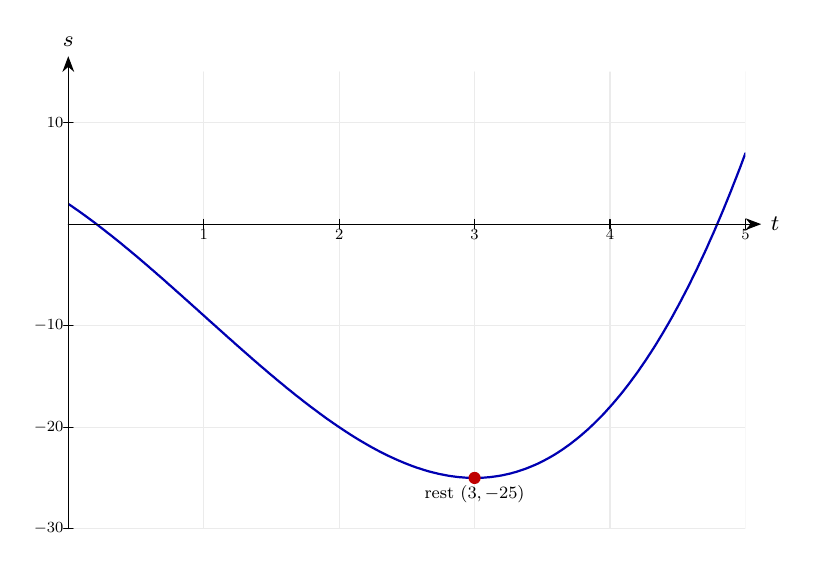
\begin{tikzpicture}[>={Stealth[length=2mm]},font=\footnotesize,line cap=round,line join=round]
\begin{scope}
\clip (0,0) rectangle (8.6,5.8);
\draw[gray!16] (0,0) grid[xstep=1.72,ystep=1.289] (8.6,5.8);
\draw[blue!70!black,thick] (0,4.124) -- (0.031,4.104) -- (0.061,4.083) -- (0.092,4.061) -- (0.123,4.04) -- (0.154,4.018) -- (0.184,3.996) -- (0.215,3.974) -- (0.246,3.951) -- (0.276,3.929) -- (0.307,3.906) -- (0.338,3.883) -- (0.369,3.859) -- (0.399,3.836) -- (0.43,3.812) -- (0.461,3.788) -- (0.491,3.764) -- (0.522,3.74) -- (0.553,3.716) -- (0.584,3.691) -- (0.614,3.667) -- (0.645,3.642) -- (0.676,3.617) -- (0.706,3.592) -- (0.737,3.566) -- (0.768,3.541) -- (0.799,3.515) -- (0.829,3.49) -- (0.86,3.464) -- (0.891,3.438) -- (0.921,3.412) -- (0.952,3.386) -- (0.983,3.359) -- (1.014,3.333) -- (1.044,3.306) -- (1.075,3.28) -- (1.106,3.253) -- (1.136,3.226) -- (1.167,3.2) -- (1.198,3.173) -- (1.229,3.146) -- (1.259,3.118) -- (1.29,3.091) -- (1.321,3.064) -- (1.351,3.037) -- (1.382,3.009) -- (1.413,2.982) -- (1.444,2.955) -- (1.474,2.927) -- (1.505,2.9) -- (1.536,2.872) -- (1.566,2.845) -- (1.597,2.817) -- (1.628,2.79) -- (1.659,2.762) -- (1.689,2.734) -- (1.72,2.707) -- (1.751,2.679) -- (1.781,2.651) -- (1.812,2.624) -- (1.843,2.596) -- (1.874,2.569) -- (1.904,2.541) -- (1.935,2.514) -- (1.966,2.486) -- (1.996,2.459) -- (2.027,2.431) -- (2.058,2.404) -- (2.089,2.377) -- (2.119,2.349) -- (2.15,2.322) -- (2.181,2.295) -- (2.211,2.268) -- (2.242,2.241) -- (2.273,2.214) -- (2.304,2.187) -- (2.334,2.16) -- (2.365,2.133) -- (2.396,2.107) -- (2.426,2.08) -- (2.457,2.054) -- (2.488,2.028) -- (2.519,2.001) -- (2.549,1.975) -- (2.58,1.949) -- (2.611,1.924) -- (2.641,1.898) -- (2.672,1.872) -- (2.703,1.847) -- (2.734,1.822) -- (2.764,1.796) -- (2.795,1.771) -- (2.826,1.747) -- (2.856,1.722) -- (2.887,1.697) -- (2.918,1.673) -- (2.949,1.649) -- (2.979,1.625) -- (3.01,1.601) -- (3.041,1.577) -- (3.071,1.554) -- (3.102,1.531) -- (3.133,1.508) -- (3.164,1.485) -- (3.194,1.462) -- (3.225,1.44) -- (3.256,1.417) -- (3.286,1.395) -- (3.317,1.374) -- (3.348,1.352) -- (3.379,1.331) -- (3.409,1.31) -- (3.44,1.289) -- (3.471,1.268) -- (3.501,1.248) -- (3.532,1.228) -- (3.563,1.208) -- (3.594,1.188) -- (3.624,1.169) -- (3.655,1.15) -- (3.686,1.131) -- (3.716,1.113) -- (3.747,1.095) -- (3.778,1.077) -- (3.809,1.059) -- (3.839,1.042) -- (3.87,1.025) -- (3.901,1.008) -- (3.931,0.992) -- (3.962,0.976) -- (3.993,0.96) -- (4.024,0.945) -- (4.054,0.93) -- (4.085,0.915) -- (4.116,0.901) -- (4.146,0.887) -- (4.177,0.873) -- (4.208,0.86) -- (4.239,0.847) -- (4.269,0.834) -- (4.3,0.822) -- (4.331,0.81) -- (4.361,0.798) -- (4.392,0.787) -- (4.423,0.776) -- (4.454,0.766) -- (4.484,0.756) -- (4.515,0.746) -- (4.546,0.737) -- (4.576,0.728) -- (4.607,0.72) -- (4.638,0.712) -- (4.669,0.705) -- (4.699,0.697) -- (4.73,0.691) -- (4.761,0.685) -- (4.791,0.679) -- (4.822,0.673) -- (4.853,0.668) -- (4.884,0.664) -- (4.914,0.66) -- (4.945,0.656) -- (4.976,0.653) -- (5.006,0.651) -- (5.037,0.648) -- (5.068,0.647) -- (5.099,0.645) -- (5.129,0.645) -- (5.16,0.644) -- (5.191,0.645) -- (5.221,0.645) -- (5.252,0.647) -- (5.283,0.648) -- (5.314,0.651) -- (5.344,0.653) -- (5.375,0.657) -- (5.406,0.661) -- (5.436,0.665) -- (5.467,0.67) -- (5.498,0.675) -- (5.529,0.681) -- (5.559,0.688) -- (5.59,0.695) -- (5.621,0.702) -- (5.651,0.711) -- (5.682,0.719) -- (5.713,0.729) -- (5.744,0.739) -- (5.774,0.749) -- (5.805,0.76) -- (5.836,0.772) -- (5.866,0.784) -- (5.897,0.797) -- (5.928,0.81) -- (5.959,0.824) -- (5.989,0.839) -- (6.02,0.854) -- (6.051,0.87) -- (6.081,0.886) -- (6.112,0.903) -- (6.143,0.921) -- (6.174,0.939) -- (6.204,0.958) -- (6.235,0.978) -- (6.266,0.998) -- (6.296,1.019) -- (6.327,1.041) -- (6.358,1.063) -- (6.389,1.086) -- (6.419,1.11) -- (6.45,1.134) -- (6.481,1.159) -- (6.511,1.184) -- (6.542,1.211) -- (6.573,1.238) -- (6.604,1.265) -- (6.634,1.294) -- (6.665,1.323) -- (6.696,1.353) -- (6.726,1.383) -- (6.757,1.414) -- (6.788,1.446) -- (6.819,1.479) -- (6.849,1.513) -- (6.88,1.547) -- (6.911,1.582) -- (6.941,1.617) -- (6.972,1.654) -- (7.003,1.691) -- (7.034,1.729) -- (7.064,1.767) -- (7.095,1.807) -- (7.126,1.847) -- (7.156,1.888) -- (7.187,1.93) -- (7.218,1.972) -- (7.249,2.015) -- (7.279,2.06) -- (7.31,2.105) -- (7.341,2.15) -- (7.371,2.197) -- (7.402,2.244) -- (7.433,2.292) -- (7.464,2.341) -- (7.494,2.391) -- (7.525,2.442) -- (7.556,2.493) -- (7.586,2.545) -- (7.617,2.598) -- (7.648,2.652) -- (7.679,2.707) -- (7.709,2.763) -- (7.74,2.819) -- (7.771,2.877) -- (7.801,2.935) -- (7.832,2.994) -- (7.863,3.054) -- (7.894,3.115) -- (7.924,3.177) -- (7.955,3.24) -- (7.986,3.303) -- (8.016,3.368) -- (8.047,3.433) -- (8.078,3.499) -- (8.109,3.566) -- (8.139,3.635) -- (8.17,3.704) -- (8.201,3.773) -- (8.231,3.844) -- (8.262,3.916) -- (8.293,3.989) -- (8.324,4.063) -- (8.354,4.137) -- (8.385,4.213) -- (8.416,4.289) -- (8.446,4.367) -- (8.477,4.445) -- (8.508,4.525) -- (8.539,4.605) -- (8.569,4.687) -- (8.6,4.769);
\end{scope}
\draw[->] (0,3.867) -- (8.8,3.867) node[right]{$t$};
\draw[->] (0,0) -- (0,6) node[above]{$s$};
\draw (1.72,3.807) -- (1.72,3.927) node[below=1pt,scale=0.7]{$1$};
\draw (3.44,3.807) -- (3.44,3.927) node[below=1pt,scale=0.7]{$2$};
\draw (5.16,3.807) -- (5.16,3.927) node[below=1pt,scale=0.7]{$3$};
\draw (6.88,3.807) -- (6.88,3.927) node[below=1pt,scale=0.7]{$4$};
\draw (8.6,3.807) -- (8.6,3.927) node[below=1pt,scale=0.7]{$5$};
\draw (-0.06,0) -- (0.06,0) node[left=1pt,scale=0.7]{$-30$};
\draw (-0.06,1.289) -- (0.06,1.289) node[left=1pt,scale=0.7]{$-20$};
\draw (-0.06,2.578) -- (0.06,2.578) node[left=1pt,scale=0.7]{$-10$};
\draw (-0.06,5.156) -- (0.06,5.156) node[left=1pt,scale=0.7]{$10$};
\fill[red!75!black] (5.16,0.644) circle (2.2pt);
\node[below,scale=0.78] at (5.16,0.644) {rest $(3,-25)$};
\end{tikzpicture}
}
\end{center}
\small The model plotted against its variable, with the key point(s) marked.\normalsize

\medskip\hrule

\section*{Real-Life Problems 31\quad\small\texttt{(d5-031)}}
\addcontentsline{toc}{section}{Real-Life Problems 31 (d5-031)}
\textit{Difficulty: Foundation \quad\textbar\quad Marks: 8}

\question{A drinks can manufacturer designs a cylindrical can of volume \( 330 \) cm\(^3\). The radius is \( r \) cm and the height is \( h \) cm. (a) Show that the total surface area (including both circular ends) is \( A = 2\pi r^2 + \dfrac{660}{r} \). (b) Find the value of \( r \) that minimises the surface area, giving your answer to 3 significant figures. (c) Find the minimum surface area to 3 significant figures.}

\textbf{Worked solution.}

\textit{Step 1: (a) Volume: \( \pi r^2 h = 330 \).}
\[\begin{gathered}
h = \frac{330}{\pi r^2}
\end{gathered}\]
Express \( h \) in terms of \( r \).

\textit{Step 2: Surface area.}
\[\begin{gathered}
A = 2\pi r^2 + 2\pi r h = 2\pi r^2 + 2\pi r \cdot \frac{330}{\pi r^2} = 2\pi r^2 + \frac{660}{r}
\end{gathered}\]
Substitute \( h \) and simplify: \( \dfrac{2\pi r \times 330}{\pi r^2} = \dfrac{660}{r} \).

\textit{Step 3: (b) Differentiate.}
\[\begin{gathered}
\frac{\mathrm{d}A}{\mathrm{d}r} = 4\pi r - \frac{660}{r^2}
\end{gathered}\]
Power rule applied to each term.

\textit{Step 4: Set to zero.}
\[\begin{gathered}
4\pi r = \frac{660}{r^2} \implies r^3 = \frac{660}{4\pi} = \frac{165}{\pi} \implies r = \sqrt[3]{\frac{165}{\pi}} \approx 3.74 \text{ cm}
\end{gathered}\]
Multiply by \( r^2 \) and solve for \( r \).

\textit{Step 5: Confirm minimum.}
\[\begin{gathered}
\frac{\mathrm{d}^2A}{\mathrm{d}r^2} = 4\pi + \frac{1320}{r^3} > 0 \Rightarrow \text{minimum}
\end{gathered}\]
Both terms are positive.

\textit{Step 6: (c) Minimum surface area.}
\[\begin{gathered}
A \approx 2\pi(3.74)^2 + \frac{660}{3.74} \approx 87.9 + 176.5 \approx 264 \text{ cm}^2
\end{gathered}\]
Substitute \( r \approx 3.74 \) into \( A \).

\begin{answerbox}
\textbf{Final answer:}\quad (a) Shown. \\[3pt]  (b) \(\displaystyle  r \approx 3.74 \) cm \\[3pt]  (c) Minimum surface area \(\displaystyle  \approx 264 \text{ cm}^2 \)
\end{answerbox}
\textbf{Diagram.}

\begin{center}
\resizebox{\ifdim\width>\linewidth \linewidth\else \width\fi}{!}{%
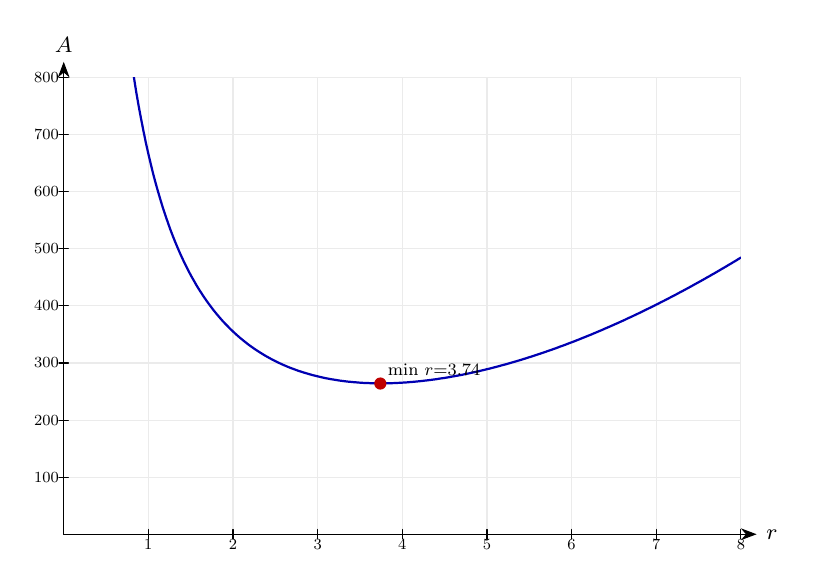
\begin{tikzpicture}[>={Stealth[length=2mm]},font=\footnotesize,line cap=round,line join=round]
\begin{scope}
\clip (0,0) rectangle (8.6,5.8);
\draw[gray!16] (0,0) grid[xstep=1.075,ystep=0.725] (8.6,5.8);
\draw[blue!70!black,thick] (0.031,11.6) -- (0.061,11.6) -- (0.092,11.6) -- (0.123,11.6) -- (0.154,11.6) -- (0.184,11.6) -- (0.215,11.6) -- (0.246,11.6) -- (0.276,11.6) -- (0.307,11.6) -- (0.338,11.6) -- (0.369,11.6) -- (0.399,11.6) -- (0.43,11.6) -- (0.461,11.173) -- (0.491,10.477) -- (0.522,9.862) -- (0.553,9.316) -- (0.584,8.828) -- (0.614,8.389) -- (0.645,7.991) -- (0.676,7.63) -- (0.706,7.301) -- (0.737,7) -- (0.768,6.722) -- (0.799,6.466) -- (0.829,6.23) -- (0.86,6.01) -- (0.891,5.806) -- (0.921,5.616) -- (0.952,5.438) -- (0.983,5.272) -- (1.014,5.115) -- (1.044,4.969) -- (1.075,4.831) -- (1.106,4.7) -- (1.136,4.577) -- (1.167,4.461) -- (1.198,4.351) -- (1.229,4.246) -- (1.259,4.147) -- (1.29,4.053) -- (1.321,3.964) -- (1.351,3.878) -- (1.382,3.797) -- (1.413,3.719) -- (1.444,3.645) -- (1.474,3.575) -- (1.505,3.507) -- (1.536,3.442) -- (1.566,3.381) -- (1.597,3.321) -- (1.628,3.264) -- (1.659,3.21) -- (1.689,3.157) -- (1.72,3.107) -- (1.751,3.059) -- (1.781,3.013) -- (1.812,2.968) -- (1.843,2.925) -- (1.874,2.884) -- (1.904,2.844) -- (1.935,2.806) -- (1.966,2.769) -- (1.996,2.734) -- (2.027,2.699) -- (2.058,2.667) -- (2.089,2.635) -- (2.119,2.604) -- (2.15,2.575) -- (2.181,2.546) -- (2.211,2.519) -- (2.242,2.492) -- (2.273,2.467) -- (2.304,2.442) -- (2.334,2.418) -- (2.365,2.395) -- (2.396,2.373) -- (2.426,2.352) -- (2.457,2.331) -- (2.488,2.312) -- (2.519,2.292) -- (2.549,2.274) -- (2.58,2.256) -- (2.611,2.239) -- (2.641,2.222) -- (2.672,2.206) -- (2.703,2.191) -- (2.734,2.176) -- (2.764,2.162) -- (2.795,2.148) -- (2.826,2.135) -- (2.856,2.122) -- (2.887,2.11) -- (2.918,2.099) -- (2.949,2.087) -- (2.979,2.076) -- (3.01,2.066) -- (3.041,2.056) -- (3.071,2.047) -- (3.102,2.038) -- (3.133,2.029) -- (3.164,2.02) -- (3.194,2.013) -- (3.225,2.005) -- (3.256,1.998) -- (3.286,1.991) -- (3.317,1.984) -- (3.348,1.978) -- (3.379,1.972) -- (3.409,1.967) -- (3.44,1.962) -- (3.471,1.957) -- (3.501,1.952) -- (3.532,1.948) -- (3.563,1.944) -- (3.594,1.94) -- (3.624,1.937) -- (3.655,1.934) -- (3.686,1.931) -- (3.716,1.929) -- (3.747,1.926) -- (3.778,1.924) -- (3.809,1.922) -- (3.839,1.921) -- (3.87,1.92) -- (3.901,1.918) -- (3.931,1.918) -- (3.962,1.917) -- (3.993,1.917) -- (4.024,1.917) -- (4.054,1.917) -- (4.085,1.917) -- (4.116,1.918) -- (4.146,1.918) -- (4.177,1.919) -- (4.208,1.92) -- (4.239,1.922) -- (4.269,1.923) -- (4.3,1.925) -- (4.331,1.927) -- (4.361,1.929) -- (4.392,1.932) -- (4.423,1.934) -- (4.454,1.937) -- (4.484,1.94) -- (4.515,1.943) -- (4.546,1.946) -- (4.576,1.95) -- (4.607,1.953) -- (4.638,1.957) -- (4.669,1.961) -- (4.699,1.965) -- (4.73,1.969) -- (4.761,1.974) -- (4.791,1.979) -- (4.822,1.983) -- (4.853,1.988) -- (4.884,1.993) -- (4.914,1.999) -- (4.945,2.004) -- (4.976,2.01) -- (5.006,2.015) -- (5.037,2.021) -- (5.068,2.027) -- (5.099,2.034) -- (5.129,2.04) -- (5.16,2.046) -- (5.191,2.053) -- (5.221,2.06) -- (5.252,2.067) -- (5.283,2.074) -- (5.314,2.081) -- (5.344,2.088) -- (5.375,2.096) -- (5.406,2.103) -- (5.436,2.111) -- (5.467,2.119) -- (5.498,2.127) -- (5.529,2.135) -- (5.559,2.144) -- (5.59,2.152) -- (5.621,2.16) -- (5.651,2.169) -- (5.682,2.178) -- (5.713,2.187) -- (5.744,2.196) -- (5.774,2.205) -- (5.805,2.214) -- (5.836,2.224) -- (5.866,2.233) -- (5.897,2.243) -- (5.928,2.253) -- (5.959,2.263) -- (5.989,2.273) -- (6.02,2.283) -- (6.051,2.293) -- (6.081,2.304) -- (6.112,2.314) -- (6.143,2.325) -- (6.174,2.336) -- (6.204,2.346) -- (6.235,2.357) -- (6.266,2.368) -- (6.296,2.38) -- (6.327,2.391) -- (6.358,2.402) -- (6.389,2.414) -- (6.419,2.426) -- (6.45,2.437) -- (6.481,2.449) -- (6.511,2.461) -- (6.542,2.473) -- (6.573,2.486) -- (6.604,2.498) -- (6.634,2.51) -- (6.665,2.523) -- (6.696,2.535) -- (6.726,2.548) -- (6.757,2.561) -- (6.788,2.574) -- (6.819,2.587) -- (6.849,2.6) -- (6.88,2.614) -- (6.911,2.627) -- (6.941,2.64) -- (6.972,2.654) -- (7.003,2.668) -- (7.034,2.681) -- (7.064,2.695) -- (7.095,2.709) -- (7.126,2.723) -- (7.156,2.738) -- (7.187,2.752) -- (7.218,2.766) -- (7.249,2.781) -- (7.279,2.795) -- (7.31,2.81) -- (7.341,2.825) -- (7.371,2.84) -- (7.402,2.855) -- (7.433,2.87) -- (7.464,2.885) -- (7.494,2.9) -- (7.525,2.916) -- (7.556,2.931) -- (7.586,2.947) -- (7.617,2.962) -- (7.648,2.978) -- (7.679,2.994) -- (7.709,3.01) -- (7.74,3.026) -- (7.771,3.042) -- (7.801,3.058) -- (7.832,3.075) -- (7.863,3.091) -- (7.894,3.108) -- (7.924,3.124) -- (7.955,3.141) -- (7.986,3.158) -- (8.016,3.175) -- (8.047,3.192) -- (8.078,3.209) -- (8.109,3.226) -- (8.139,3.243) -- (8.17,3.261) -- (8.201,3.278) -- (8.231,3.296) -- (8.262,3.313) -- (8.293,3.331) -- (8.324,3.349) -- (8.354,3.367) -- (8.385,3.385) -- (8.416,3.403) -- (8.446,3.421) -- (8.477,3.439) -- (8.508,3.458) -- (8.539,3.476) -- (8.569,3.495) -- (8.6,3.514);
\end{scope}
\draw[->] (0,0) -- (8.8,0) node[right]{$r$};
\draw[->] (0,0) -- (0,6) node[above]{$A$};
\draw (1.075,-0.06) -- (1.075,0.06) node[below=1pt,scale=0.7]{$1$};
\draw (2.15,-0.06) -- (2.15,0.06) node[below=1pt,scale=0.7]{$2$};
\draw (3.225,-0.06) -- (3.225,0.06) node[below=1pt,scale=0.7]{$3$};
\draw (4.3,-0.06) -- (4.3,0.06) node[below=1pt,scale=0.7]{$4$};
\draw (5.375,-0.06) -- (5.375,0.06) node[below=1pt,scale=0.7]{$5$};
\draw (6.45,-0.06) -- (6.45,0.06) node[below=1pt,scale=0.7]{$6$};
\draw (7.525,-0.06) -- (7.525,0.06) node[below=1pt,scale=0.7]{$7$};
\draw (8.6,-0.06) -- (8.6,0.06) node[below=1pt,scale=0.7]{$8$};
\draw (-0.06,0.725) -- (0.06,0.725) node[left=1pt,scale=0.7]{$100$};
\draw (-0.06,1.45) -- (0.06,1.45) node[left=1pt,scale=0.7]{$200$};
\draw (-0.06,2.175) -- (0.06,2.175) node[left=1pt,scale=0.7]{$300$};
\draw (-0.06,2.9) -- (0.06,2.9) node[left=1pt,scale=0.7]{$400$};
\draw (-0.06,3.625) -- (0.06,3.625) node[left=1pt,scale=0.7]{$500$};
\draw (-0.06,4.35) -- (0.06,4.35) node[left=1pt,scale=0.7]{$600$};
\draw (-0.06,5.075) -- (0.06,5.075) node[left=1pt,scale=0.7]{$700$};
\draw (-0.06,5.8) -- (0.06,5.8) node[left=1pt,scale=0.7]{$800$};
\fill[red!75!black] (4.021,1.914) circle (2.2pt);
\node[above right,scale=0.78] at (4.021,1.914) {min $r{=}3.74$};
\end{tikzpicture}
}
\end{center}
\small The model plotted against its variable, with the key point(s) marked.\normalsize

\medskip\hrule

\section*{Real-Life Problems 32\quad\small\texttt{(d5-032)}}
\addcontentsline{toc}{section}{Real-Life Problems 32 (d5-032)}
\textit{Difficulty: Foundation \quad\textbar\quad Marks: 7}

\question{A particle moves along a straight line so that its displacement \( s \) metres at time \( t \) seconds is \( s = 2t^3 - 5t^2 + 4t \) for \( t \geq 0 \). (a) Find the velocity function and determine when the particle first comes to rest. (b) Find the acceleration at that instant. (c) Determine whether the particle is speeding up or slowing down just before it comes to rest.}

\textbf{Worked solution.}

\textit{Step 1: (a) Velocity.}
\[\begin{gathered}
v = 6t^2 - 10t + 4
\end{gathered}\]
Differentiate \( s \).

\textit{Step 2: Set \( v = 0 \).}
\[\begin{gathered}
6t^2 - 10t + 4 = 0 \implies 3t^2 - 5t + 2 = 0 \implies (3t - 2)(t - 1) = 0
\end{gathered}\]
Divide by 2 and factorise.

\textit{Step 3: First time at rest.}
\[\begin{gathered}
t = \tfrac{2}{3} \text{ s (earlier root)}
\end{gathered}\]
\( t = \tfrac{2}{3} < 1 \), so the particle first comes to rest at \( t = \tfrac{2}{3} \) s.

\textit{Step 4: (b) Acceleration.}
\[\begin{gathered}
a = 12t - 10; \quad a\!\left(\tfrac{2}{3}\right) = 8 - 10 = -2 \text{ ms}^{-2}
\end{gathered}\]
Differentiate \( v \) and substitute \( t = \tfrac{2}{3} \).

\textit{Step 5: (c) Just before \( t = \tfrac{2}{3} \), check the sign of \( v \).}
\[\begin{gathered}
v(0.5) = 6(0.25) - 10(0.5) + 4 = 1.5 - 5 + 4 = 0.5 > 0
\end{gathered}\]
The particle is moving in the positive direction. The acceleration is \(-2 \text{ ms}^{-2}\) (opposing the motion), so the particle is slowing down.

\begin{answerbox}
\textbf{Final answer:}\quad (a) \(\displaystyle  v = 6t^2-10t+4 \); first at rest at \(\displaystyle  t = \tfrac{2}{3} \) s \\[3pt]  (b) \(\displaystyle  a = -2 \text{ ms}^{-2} \) \\[3pt]  (c) Slowing down (velocity positive, acceleration negative)
\end{answerbox}
\textbf{Diagram.}

\begin{center}
\resizebox{\ifdim\width>\linewidth \linewidth\else \width\fi}{!}{%
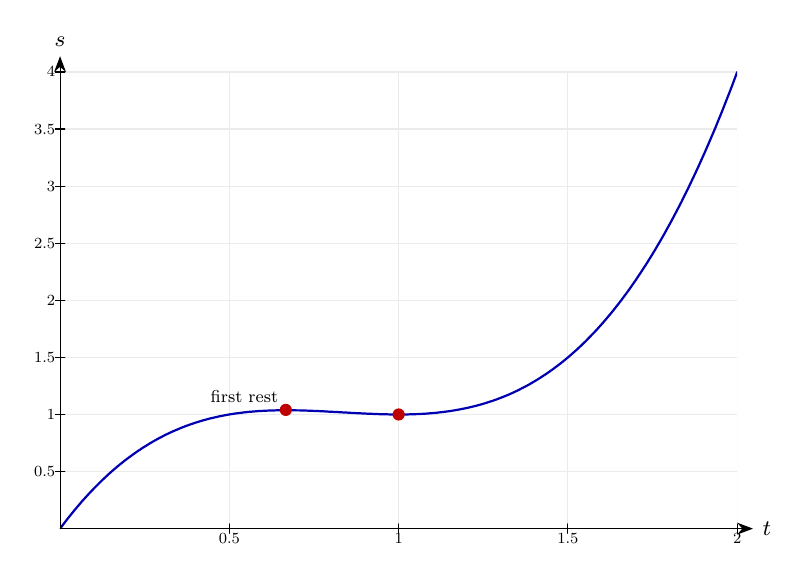
\begin{tikzpicture}[>={Stealth[length=2mm]},font=\footnotesize,line cap=round,line join=round]
\begin{scope}
\clip (0,0) rectangle (8.6,5.8);
\draw[gray!16] (0,0) grid[xstep=2.15,ystep=0.725] (8.6,5.8);
\draw[blue!70!black,thick] (0,0) -- (0.031,0.041) -- (0.061,0.081) -- (0.092,0.121) -- (0.123,0.16) -- (0.154,0.198) -- (0.184,0.235) -- (0.215,0.272) -- (0.246,0.308) -- (0.276,0.344) -- (0.307,0.378) -- (0.338,0.412) -- (0.369,0.446) -- (0.399,0.478) -- (0.43,0.51) -- (0.461,0.542) -- (0.491,0.572) -- (0.522,0.603) -- (0.553,0.632) -- (0.584,0.661) -- (0.614,0.689) -- (0.645,0.717) -- (0.676,0.744) -- (0.706,0.77) -- (0.737,0.796) -- (0.768,0.821) -- (0.799,0.846) -- (0.829,0.87) -- (0.86,0.893) -- (0.891,0.916) -- (0.921,0.938) -- (0.952,0.96) -- (0.983,0.982) -- (1.014,1.002) -- (1.044,1.023) -- (1.075,1.042) -- (1.106,1.061) -- (1.136,1.08) -- (1.167,1.098) -- (1.198,1.116) -- (1.229,1.133) -- (1.259,1.15) -- (1.29,1.166) -- (1.321,1.182) -- (1.351,1.197) -- (1.382,1.212) -- (1.413,1.226) -- (1.444,1.24) -- (1.474,1.253) -- (1.505,1.266) -- (1.536,1.279) -- (1.566,1.291) -- (1.597,1.303) -- (1.628,1.314) -- (1.659,1.325) -- (1.689,1.335) -- (1.72,1.346) -- (1.751,1.355) -- (1.781,1.365) -- (1.812,1.374) -- (1.843,1.382) -- (1.874,1.391) -- (1.904,1.399) -- (1.935,1.406) -- (1.966,1.413) -- (1.996,1.42) -- (2.027,1.427) -- (2.058,1.433) -- (2.089,1.439) -- (2.119,1.445) -- (2.15,1.45) -- (2.181,1.455) -- (2.211,1.46) -- (2.242,1.464) -- (2.273,1.468) -- (2.304,1.472) -- (2.334,1.476) -- (2.365,1.479) -- (2.396,1.483) -- (2.426,1.485) -- (2.457,1.488) -- (2.488,1.49) -- (2.519,1.493) -- (2.549,1.495) -- (2.58,1.496) -- (2.611,1.498) -- (2.641,1.499) -- (2.672,1.5) -- (2.703,1.501) -- (2.734,1.502) -- (2.764,1.503) -- (2.795,1.503) -- (2.826,1.504) -- (2.856,1.504) -- (2.887,1.504) -- (2.918,1.504) -- (2.949,1.503) -- (2.979,1.503) -- (3.01,1.502) -- (3.041,1.502) -- (3.071,1.501) -- (3.102,1.5) -- (3.133,1.499) -- (3.164,1.498) -- (3.194,1.497) -- (3.225,1.495) -- (3.256,1.494) -- (3.286,1.493) -- (3.317,1.491) -- (3.348,1.49) -- (3.379,1.488) -- (3.409,1.486) -- (3.44,1.485) -- (3.471,1.483) -- (3.501,1.481) -- (3.532,1.48) -- (3.563,1.478) -- (3.594,1.476) -- (3.624,1.475) -- (3.655,1.473) -- (3.686,1.471) -- (3.716,1.469) -- (3.747,1.468) -- (3.778,1.466) -- (3.809,1.465) -- (3.839,1.463) -- (3.87,1.462) -- (3.901,1.46) -- (3.931,1.459) -- (3.962,1.458) -- (3.993,1.456) -- (4.024,1.455) -- (4.054,1.454) -- (4.085,1.453) -- (4.116,1.452) -- (4.146,1.452) -- (4.177,1.451) -- (4.208,1.451) -- (4.239,1.45) -- (4.269,1.45) -- (4.3,1.45) -- (4.331,1.45) -- (4.361,1.45) -- (4.392,1.451) -- (4.423,1.451) -- (4.454,1.452) -- (4.484,1.453) -- (4.515,1.454) -- (4.546,1.455) -- (4.576,1.457) -- (4.607,1.458) -- (4.638,1.46) -- (4.669,1.462) -- (4.699,1.465) -- (4.73,1.467) -- (4.761,1.47) -- (4.791,1.473) -- (4.822,1.477) -- (4.853,1.48) -- (4.884,1.484) -- (4.914,1.488) -- (4.945,1.492) -- (4.976,1.497) -- (5.006,1.502) -- (5.037,1.507) -- (5.068,1.513) -- (5.099,1.519) -- (5.129,1.525) -- (5.16,1.531) -- (5.191,1.538) -- (5.221,1.545) -- (5.252,1.553) -- (5.283,1.56) -- (5.314,1.569) -- (5.344,1.577) -- (5.375,1.586) -- (5.406,1.595) -- (5.436,1.605) -- (5.467,1.615) -- (5.498,1.625) -- (5.529,1.636) -- (5.559,1.647) -- (5.59,1.659) -- (5.621,1.671) -- (5.651,1.683) -- (5.682,1.696) -- (5.713,1.709) -- (5.744,1.723) -- (5.774,1.737) -- (5.805,1.752) -- (5.836,1.767) -- (5.866,1.783) -- (5.897,1.799) -- (5.928,1.815) -- (5.959,1.832) -- (5.989,1.85) -- (6.02,1.868) -- (6.051,1.886) -- (6.081,1.905) -- (6.112,1.925) -- (6.143,1.945) -- (6.174,1.965) -- (6.204,1.986) -- (6.235,2.008) -- (6.266,2.03) -- (6.296,2.053) -- (6.327,2.076) -- (6.358,2.1) -- (6.389,2.124) -- (6.419,2.149) -- (6.45,2.175) -- (6.481,2.201) -- (6.511,2.228) -- (6.542,2.255) -- (6.573,2.283) -- (6.604,2.312) -- (6.634,2.341) -- (6.665,2.371) -- (6.696,2.402) -- (6.726,2.433) -- (6.757,2.465) -- (6.788,2.497) -- (6.819,2.53) -- (6.849,2.564) -- (6.88,2.598) -- (6.911,2.634) -- (6.941,2.669) -- (6.972,2.706) -- (7.003,2.743) -- (7.034,2.781) -- (7.064,2.82) -- (7.095,2.859) -- (7.126,2.899) -- (7.156,2.94) -- (7.187,2.981) -- (7.218,3.024) -- (7.249,3.067) -- (7.279,3.111) -- (7.31,3.155) -- (7.341,3.201) -- (7.371,3.247) -- (7.402,3.294) -- (7.433,3.341) -- (7.464,3.39) -- (7.494,3.439) -- (7.525,3.489) -- (7.556,3.54) -- (7.586,3.592) -- (7.617,3.644) -- (7.648,3.698) -- (7.679,3.752) -- (7.709,3.807) -- (7.74,3.863) -- (7.771,3.92) -- (7.801,3.977) -- (7.832,4.036) -- (7.863,4.095) -- (7.894,4.155) -- (7.924,4.217) -- (7.955,4.279) -- (7.986,4.342) -- (8.016,4.405) -- (8.047,4.47) -- (8.078,4.536) -- (8.109,4.603) -- (8.139,4.67) -- (8.17,4.739) -- (8.201,4.808) -- (8.231,4.878) -- (8.262,4.95) -- (8.293,5.022) -- (8.324,5.095) -- (8.354,5.17) -- (8.385,5.245) -- (8.416,5.321) -- (8.446,5.399) -- (8.477,5.477) -- (8.508,5.556) -- (8.539,5.636) -- (8.569,5.718) -- (8.6,5.8);
\end{scope}
\draw[->] (0,0) -- (8.8,0) node[right]{$t$};
\draw[->] (0,0) -- (0,6) node[above]{$s$};
\draw (2.15,-0.06) -- (2.15,0.06) node[below=1pt,scale=0.7]{$0.5$};
\draw (4.3,-0.06) -- (4.3,0.06) node[below=1pt,scale=0.7]{$1$};
\draw (6.45,-0.06) -- (6.45,0.06) node[below=1pt,scale=0.7]{$1.5$};
\draw (8.6,-0.06) -- (8.6,0.06) node[below=1pt,scale=0.7]{$2$};
\draw (-0.06,0.725) -- (0.06,0.725) node[left=1pt,scale=0.7]{$0.5$};
\draw (-0.06,1.45) -- (0.06,1.45) node[left=1pt,scale=0.7]{$1$};
\draw (-0.06,2.175) -- (0.06,2.175) node[left=1pt,scale=0.7]{$1.5$};
\draw (-0.06,2.9) -- (0.06,2.9) node[left=1pt,scale=0.7]{$2$};
\draw (-0.06,3.625) -- (0.06,3.625) node[left=1pt,scale=0.7]{$2.5$};
\draw (-0.06,4.35) -- (0.06,4.35) node[left=1pt,scale=0.7]{$3$};
\draw (-0.06,5.075) -- (0.06,5.075) node[left=1pt,scale=0.7]{$3.5$};
\draw (-0.06,5.8) -- (0.06,5.8) node[left=1pt,scale=0.7]{$4$};
\fill[red!75!black] (2.867,1.508) circle (2.2pt);
\node[above left,scale=0.78] at (2.867,1.508) {first rest};
\fill[red!75!black] (4.3,1.45) circle (2.2pt);
\end{tikzpicture}
}
\end{center}
\small The model plotted against its variable, with the key point(s) marked.\normalsize

\medskip\hrule

\section*{Real-Life Problems 33\quad\small\texttt{(d5-033)}}
\addcontentsline{toc}{section}{Real-Life Problems 33 (d5-033)}
\textit{Difficulty: Foundation \quad\textbar\quad Marks: 8}

\question{An architect designs a Norman window consisting of a rectangle surmounted by a semicircle. The perimeter of the window (including the base) is \( 6 \) m and the width of the rectangle is \( 2r \) m. (a) Show that the height of the rectangular part is \( h = 3 - r - \dfrac{\pi r}{2} \). (b) Show that the total area is \( A = 6r - 2r^2 - \dfrac{\pi r^2}{2} \). (c) Find the value of \( r \) that maximises the area, giving your answer in exact form.}

\textbf{Worked solution.}

\textit{Step 1: (a) Perimeter: base \( + \) two sides \( + \) semicircle arc.}
\[\begin{gathered}
2r + 2h + \pi r = 6 \implies 2h = 6 - 2r - \pi r \implies h = 3 - r - \frac{\pi r}{2}
\end{gathered}\]
The semicircle arc has length \( \pi r \) (half the circumference of a circle of radius \( r \)).

\textit{Step 2: (b) Total area = rectangle + semicircle.}
\[\begin{gathered}
A = 2rh + \frac{\pi r^2}{2} = 2r\!\left(3 - r - \frac{\pi r}{2}\right) + \frac{\pi r^2}{2}
\end{gathered}\]
Substitute \( h \) into the area expression.

\textit{Step 3: Expand.}
\[\begin{gathered}
A = 6r - 2r^2 - \pi r^2 + \frac{\pi r^2}{2} = 6r - 2r^2 - \frac{\pi r^2}{2}
\end{gathered}\]
\( -\pi r^2 + \dfrac{\pi r^2}{2} = -\dfrac{\pi r^2}{2} \).

\textit{Step 4: (c) Differentiate.}
\[\begin{gathered}
\frac{\mathrm{d}A}{\mathrm{d}r} = 6 - 4r - \pi r = 6 - r(4 + \pi)
\end{gathered}\]
Power rule.

\textit{Step 5: Set to zero.}
\[\begin{gathered}
r(4 + \pi) = 6 \implies r = \frac{6}{4 + \pi}
\end{gathered}\]
This is the exact value.

\textit{Step 6: Confirm maximum.}
\[\begin{gathered}
\frac{\mathrm{d}^2A}{\mathrm{d}r^2} = -(4 + \pi) < 0 \Rightarrow \text{maximum}
\end{gathered}\]
Negative second derivative.

\begin{answerbox}
\textbf{Final answer:}\quad (a) Shown. \\[3pt]  (b) Shown. \\[3pt]  (c) \(\displaystyle  r = \dfrac{6}{4 + \pi} \) m
\end{answerbox}
\textbf{Diagram.}

\begin{center}
\resizebox{\ifdim\width>\linewidth \linewidth\else \width\fi}{!}{%
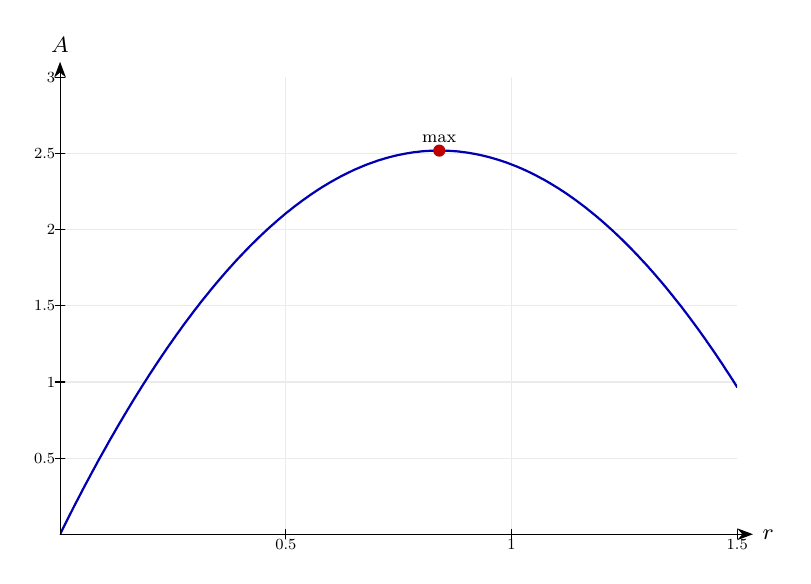
\begin{tikzpicture}[>={Stealth[length=2mm]},font=\footnotesize,line cap=round,line join=round]
\begin{scope}
\clip (0,0) rectangle (8.6,5.8);
\draw[gray!16] (0,0) grid[xstep=2.867,ystep=0.967] (8.6,5.8);
\draw[blue!70!black,thick] (0,0) -- (0.031,0.062) -- (0.061,0.123) -- (0.092,0.185) -- (0.123,0.245) -- (0.154,0.306) -- (0.184,0.366) -- (0.215,0.425) -- (0.246,0.484) -- (0.276,0.543) -- (0.307,0.602) -- (0.338,0.66) -- (0.369,0.717) -- (0.399,0.774) -- (0.43,0.831) -- (0.461,0.888) -- (0.491,0.944) -- (0.522,0.999) -- (0.553,1.054) -- (0.584,1.109) -- (0.614,1.164) -- (0.645,1.218) -- (0.676,1.271) -- (0.706,1.324) -- (0.737,1.377) -- (0.768,1.43) -- (0.799,1.482) -- (0.829,1.533) -- (0.86,1.585) -- (0.891,1.636) -- (0.921,1.686) -- (0.952,1.736) -- (0.983,1.786) -- (1.014,1.835) -- (1.044,1.884) -- (1.075,1.932) -- (1.106,1.98) -- (1.136,2.028) -- (1.167,2.075) -- (1.198,2.122) -- (1.229,2.169) -- (1.259,2.215) -- (1.29,2.261) -- (1.321,2.306) -- (1.351,2.351) -- (1.382,2.395) -- (1.413,2.439) -- (1.444,2.483) -- (1.474,2.526) -- (1.505,2.569) -- (1.536,2.612) -- (1.566,2.654) -- (1.597,2.696) -- (1.628,2.737) -- (1.659,2.778) -- (1.689,2.819) -- (1.72,2.859) -- (1.751,2.898) -- (1.781,2.938) -- (1.812,2.977) -- (1.843,3.015) -- (1.874,3.053) -- (1.904,3.091) -- (1.935,3.129) -- (1.966,3.166) -- (1.996,3.202) -- (2.027,3.238) -- (2.058,3.274) -- (2.089,3.31) -- (2.119,3.345) -- (2.15,3.379) -- (2.181,3.413) -- (2.211,3.447) -- (2.242,3.481) -- (2.273,3.514) -- (2.304,3.546) -- (2.334,3.578) -- (2.365,3.61) -- (2.396,3.642) -- (2.426,3.673) -- (2.457,3.703) -- (2.488,3.734) -- (2.519,3.764) -- (2.549,3.793) -- (2.58,3.822) -- (2.611,3.851) -- (2.641,3.879) -- (2.672,3.907) -- (2.703,3.934) -- (2.734,3.961) -- (2.764,3.988) -- (2.795,4.014) -- (2.826,4.04) -- (2.856,4.066) -- (2.887,4.091) -- (2.918,4.115) -- (2.949,4.14) -- (2.979,4.164) -- (3.01,4.187) -- (3.041,4.21) -- (3.071,4.233) -- (3.102,4.255) -- (3.133,4.277) -- (3.164,4.299) -- (3.194,4.32) -- (3.225,4.341) -- (3.256,4.361) -- (3.286,4.381) -- (3.317,4.401) -- (3.348,4.42) -- (3.379,4.438) -- (3.409,4.457) -- (3.44,4.475) -- (3.471,4.492) -- (3.501,4.509) -- (3.532,4.526) -- (3.563,4.543) -- (3.594,4.559) -- (3.624,4.574) -- (3.655,4.589) -- (3.686,4.604) -- (3.716,4.619) -- (3.747,4.633) -- (3.778,4.646) -- (3.809,4.659) -- (3.839,4.672) -- (3.87,4.685) -- (3.901,4.697) -- (3.931,4.708) -- (3.962,4.719) -- (3.993,4.73) -- (4.024,4.741) -- (4.054,4.751) -- (4.085,4.76) -- (4.116,4.77) -- (4.146,4.778) -- (4.177,4.787) -- (4.208,4.795) -- (4.239,4.803) -- (4.269,4.81) -- (4.3,4.817) -- (4.331,4.823) -- (4.361,4.829) -- (4.392,4.835) -- (4.423,4.84) -- (4.454,4.845) -- (4.484,4.85) -- (4.515,4.854) -- (4.546,4.857) -- (4.576,4.861) -- (4.607,4.864) -- (4.638,4.866) -- (4.669,4.868) -- (4.699,4.87) -- (4.73,4.871) -- (4.761,4.872) -- (4.791,4.873) -- (4.822,4.873) -- (4.853,4.873) -- (4.884,4.872) -- (4.914,4.871) -- (4.945,4.869) -- (4.976,4.868) -- (5.006,4.865) -- (5.037,4.863) -- (5.068,4.86) -- (5.099,4.856) -- (5.129,4.852) -- (5.16,4.848) -- (5.191,4.844) -- (5.221,4.838) -- (5.252,4.833) -- (5.283,4.827) -- (5.314,4.821) -- (5.344,4.814) -- (5.375,4.807) -- (5.406,4.8) -- (5.436,4.792) -- (5.467,4.784) -- (5.498,4.775) -- (5.529,4.766) -- (5.559,4.757) -- (5.59,4.747) -- (5.621,4.737) -- (5.651,4.727) -- (5.682,4.716) -- (5.713,4.704) -- (5.744,4.692) -- (5.774,4.68) -- (5.805,4.668) -- (5.836,4.655) -- (5.866,4.642) -- (5.897,4.628) -- (5.928,4.614) -- (5.959,4.599) -- (5.989,4.584) -- (6.02,4.569) -- (6.051,4.553) -- (6.081,4.537) -- (6.112,4.52) -- (6.143,4.504) -- (6.174,4.486) -- (6.204,4.469) -- (6.235,4.45) -- (6.266,4.432) -- (6.296,4.413) -- (6.327,4.394) -- (6.358,4.374) -- (6.389,4.354) -- (6.419,4.334) -- (6.45,4.313) -- (6.481,4.291) -- (6.511,4.27) -- (6.542,4.248) -- (6.573,4.225) -- (6.604,4.202) -- (6.634,4.179) -- (6.665,4.156) -- (6.696,4.131) -- (6.726,4.107) -- (6.757,4.082) -- (6.788,4.057) -- (6.819,4.031) -- (6.849,4.005) -- (6.88,3.979) -- (6.911,3.952) -- (6.941,3.925) -- (6.972,3.897) -- (7.003,3.869) -- (7.034,3.841) -- (7.064,3.812) -- (7.095,3.783) -- (7.126,3.753) -- (7.156,3.723) -- (7.187,3.693) -- (7.218,3.662) -- (7.249,3.631) -- (7.279,3.599) -- (7.31,3.567) -- (7.341,3.535) -- (7.371,3.502) -- (7.402,3.469) -- (7.433,3.436) -- (7.464,3.402) -- (7.494,3.367) -- (7.525,3.333) -- (7.556,3.297) -- (7.586,3.262) -- (7.617,3.226) -- (7.648,3.19) -- (7.679,3.153) -- (7.709,3.116) -- (7.74,3.078) -- (7.771,3.04) -- (7.801,3.002) -- (7.832,2.963) -- (7.863,2.924) -- (7.894,2.885) -- (7.924,2.845) -- (7.955,2.805) -- (7.986,2.764) -- (8.016,2.723) -- (8.047,2.681) -- (8.078,2.639) -- (8.109,2.597) -- (8.139,2.555) -- (8.17,2.511) -- (8.201,2.468) -- (8.231,2.424) -- (8.262,2.38) -- (8.293,2.335) -- (8.324,2.29) -- (8.354,2.245) -- (8.385,2.199) -- (8.416,2.153) -- (8.446,2.106) -- (8.477,2.059) -- (8.508,2.012) -- (8.539,1.964) -- (8.569,1.916) -- (8.6,1.867);
\end{scope}
\draw[->] (0,0) -- (8.8,0) node[right]{$r$};
\draw[->] (0,0) -- (0,6) node[above]{$A$};
\draw (2.867,-0.06) -- (2.867,0.06) node[below=1pt,scale=0.7]{$0.5$};
\draw (5.733,-0.06) -- (5.733,0.06) node[below=1pt,scale=0.7]{$1$};
\draw (8.6,-0.06) -- (8.6,0.06) node[below=1pt,scale=0.7]{$1.5$};
\draw (-0.06,0.967) -- (0.06,0.967) node[left=1pt,scale=0.7]{$0.5$};
\draw (-0.06,1.933) -- (0.06,1.933) node[left=1pt,scale=0.7]{$1$};
\draw (-0.06,2.9) -- (0.06,2.9) node[left=1pt,scale=0.7]{$1.5$};
\draw (-0.06,3.867) -- (0.06,3.867) node[left=1pt,scale=0.7]{$2$};
\draw (-0.06,4.833) -- (0.06,4.833) node[left=1pt,scale=0.7]{$2.5$};
\draw (-0.06,5.8) -- (0.06,5.8) node[left=1pt,scale=0.7]{$3$};
\fill[red!75!black] (4.816,4.872) circle (2.2pt);
\node[above,scale=0.78] at (4.816,4.872) {max};
\end{tikzpicture}
}
\end{center}
\small The model plotted against its variable, with the key point(s) marked.\normalsize

\medskip\hrule

\section*{Real-Life Problems 34\quad\small\texttt{(d5-034)}}
\addcontentsline{toc}{section}{Real-Life Problems 34 (d5-034)}
\textit{Difficulty: Foundation \quad\textbar\quad Marks: 8}

\question{A particle \( P \) moves along the \( x \)-axis. Its displacement from the origin \( O \) at time \( t \) seconds is \( x = t^3 - 12t + 4 \) metres for \( t \geq 0 \). (a) Find \( \dfrac{\mathrm{d}x}{\mathrm{d}t} \) and \( \dfrac{\mathrm{d}^2x}{\mathrm{d}t^2} \). (b) Find the times when \( P \) is at rest. (c) Find the position of \( P \) at each of those times. (d) Determine the direction \( P \) is travelling just after \( t = 2 \).}

\textbf{Worked solution.}

\textit{Step 1: (a) Velocity.}
\[\begin{gathered}
\frac{\mathrm{d}x}{\mathrm{d}t} = 3t^2 - 12
\end{gathered}\]
Power rule.

\textit{Step 2: Acceleration.}
\[\begin{gathered}
\frac{\mathrm{d}^2x}{\mathrm{d}t^2} = 6t
\end{gathered}\]
Differentiate the velocity.

\textit{Step 3: (b) Set velocity to zero.}
\[\begin{gathered}
3t^2 - 12 = 0 \implies t^2 = 4 \implies t = 2 \text{ s (reject } t=-2\text{)}
\end{gathered}\]
Only \( t = 2 \) is valid for \( t \geq 0 \).

\textit{Step 4: (c) Position at \( t = 2 \).}
\[\begin{gathered}
x(2) = 8 - 24 + 4 = -12 \text{ m}
\end{gathered}\]
Particle is 12 m on the negative side of \( O \).

\textit{Step 5: (d) Just after \( t = 2 \), check the sign of \( v \) at, say, \( t = 2.1 \).}
\[\begin{gathered}
v(2.1) = 3(4.41) - 12 = 13.23 - 12 = 1.23 > 0
\end{gathered}\]
Positive velocity means the particle moves in the positive direction (towards \( O \) and beyond) just after \( t = 2 \).

\begin{answerbox}
\textbf{Final answer:}\quad (a) \(\displaystyle  \dfrac{\mathrm{d}x}{\mathrm{d}t} = 3t^2 - 12 \), \(\displaystyle  \dfrac{\mathrm{d}^2x}{\mathrm{d}t^2} = 6t \) \\[3pt]  (b) \(\displaystyle  t = 2 \) s \\[3pt]  (c) \(\displaystyle  x = -12 \) m \\[3pt]  (d) Positive direction
\end{answerbox}
\textbf{Diagram.}

\begin{center}
\resizebox{\ifdim\width>\linewidth \linewidth\else \width\fi}{!}{%
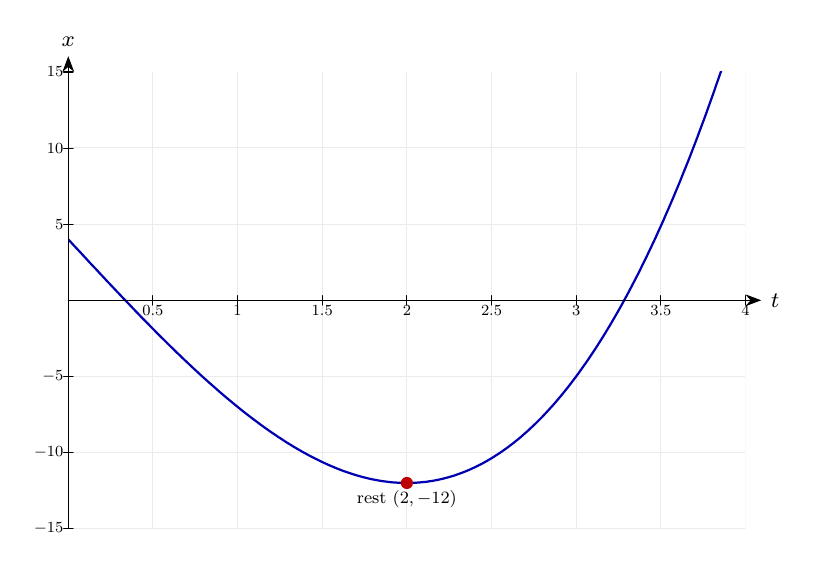
\begin{tikzpicture}[>={Stealth[length=2mm]},font=\footnotesize,line cap=round,line join=round]
\begin{scope}
\clip (0,0) rectangle (8.6,5.8);
\draw[gray!16] (0,0) grid[xstep=1.075,ystep=0.967] (8.6,5.8);
\draw[blue!70!black,thick] (0,3.673) -- (0.031,3.64) -- (0.061,3.607) -- (0.092,3.574) -- (0.123,3.541) -- (0.154,3.508) -- (0.184,3.475) -- (0.215,3.442) -- (0.246,3.408) -- (0.276,3.375) -- (0.307,3.342) -- (0.338,3.31) -- (0.369,3.277) -- (0.399,3.244) -- (0.43,3.211) -- (0.461,3.178) -- (0.491,3.145) -- (0.522,3.113) -- (0.553,3.08) -- (0.584,3.047) -- (0.614,3.015) -- (0.645,2.983) -- (0.676,2.95) -- (0.706,2.918) -- (0.737,2.886) -- (0.768,2.854) -- (0.799,2.822) -- (0.829,2.79) -- (0.86,2.758) -- (0.891,2.726) -- (0.921,2.694) -- (0.952,2.663) -- (0.983,2.631) -- (1.014,2.6) -- (1.044,2.569) -- (1.075,2.538) -- (1.106,2.506) -- (1.136,2.476) -- (1.167,2.445) -- (1.198,2.414) -- (1.229,2.384) -- (1.259,2.353) -- (1.29,2.323) -- (1.321,2.293) -- (1.351,2.263) -- (1.382,2.233) -- (1.413,2.204) -- (1.444,2.174) -- (1.474,2.145) -- (1.505,2.116) -- (1.536,2.087) -- (1.566,2.058) -- (1.597,2.029) -- (1.628,2.001) -- (1.659,1.972) -- (1.689,1.944) -- (1.72,1.916) -- (1.751,1.889) -- (1.781,1.861) -- (1.812,1.834) -- (1.843,1.807) -- (1.874,1.78) -- (1.904,1.753) -- (1.935,1.726) -- (1.966,1.7) -- (1.996,1.674) -- (2.027,1.648) -- (2.058,1.622) -- (2.089,1.597) -- (2.119,1.572) -- (2.15,1.547) -- (2.181,1.522) -- (2.211,1.497) -- (2.242,1.473) -- (2.273,1.449) -- (2.304,1.425) -- (2.334,1.402) -- (2.365,1.379) -- (2.396,1.356) -- (2.426,1.333) -- (2.457,1.31) -- (2.488,1.288) -- (2.519,1.266) -- (2.549,1.245) -- (2.58,1.223) -- (2.611,1.202) -- (2.641,1.182) -- (2.672,1.161) -- (2.703,1.141) -- (2.734,1.121) -- (2.764,1.101) -- (2.795,1.082) -- (2.826,1.063) -- (2.856,1.044) -- (2.887,1.026) -- (2.918,1.008) -- (2.949,0.99) -- (2.979,0.973) -- (3.01,0.956) -- (3.041,0.939) -- (3.071,0.923) -- (3.102,0.907) -- (3.133,0.891) -- (3.164,0.876) -- (3.194,0.861) -- (3.225,0.846) -- (3.256,0.832) -- (3.286,0.818) -- (3.317,0.804) -- (3.348,0.791) -- (3.379,0.778) -- (3.409,0.765) -- (3.44,0.753) -- (3.471,0.741) -- (3.501,0.73) -- (3.532,0.719) -- (3.563,0.709) -- (3.594,0.698) -- (3.624,0.689) -- (3.655,0.679) -- (3.686,0.67) -- (3.716,0.662) -- (3.747,0.653) -- (3.778,0.646) -- (3.809,0.638) -- (3.839,0.631) -- (3.87,0.625) -- (3.901,0.619) -- (3.931,0.613) -- (3.962,0.608) -- (3.993,0.603) -- (4.024,0.599) -- (4.054,0.595) -- (4.085,0.591) -- (4.116,0.588) -- (4.146,0.586) -- (4.177,0.584) -- (4.208,0.582) -- (4.239,0.581) -- (4.269,0.58) -- (4.3,0.58) -- (4.331,0.58) -- (4.361,0.581) -- (4.392,0.582) -- (4.423,0.584) -- (4.454,0.586) -- (4.484,0.589) -- (4.515,0.592) -- (4.546,0.595) -- (4.576,0.6) -- (4.607,0.604) -- (4.638,0.609) -- (4.669,0.615) -- (4.699,0.621) -- (4.73,0.628) -- (4.761,0.635) -- (4.791,0.643) -- (4.822,0.651) -- (4.853,0.66) -- (4.884,0.669) -- (4.914,0.679) -- (4.945,0.69) -- (4.976,0.701) -- (5.006,0.712) -- (5.037,0.724) -- (5.068,0.737) -- (5.099,0.75) -- (5.129,0.764) -- (5.16,0.778) -- (5.191,0.793) -- (5.221,0.808) -- (5.252,0.824) -- (5.283,0.841) -- (5.314,0.858) -- (5.344,0.876) -- (5.375,0.894) -- (5.406,0.913) -- (5.436,0.933) -- (5.467,0.953) -- (5.498,0.974) -- (5.529,0.995) -- (5.559,1.017) -- (5.59,1.039) -- (5.621,1.063) -- (5.651,1.086) -- (5.682,1.111) -- (5.713,1.136) -- (5.744,1.161) -- (5.774,1.188) -- (5.805,1.215) -- (5.836,1.242) -- (5.866,1.271) -- (5.897,1.299) -- (5.928,1.329) -- (5.959,1.359) -- (5.989,1.39) -- (6.02,1.421) -- (6.051,1.454) -- (6.081,1.486) -- (6.112,1.52) -- (6.143,1.554) -- (6.174,1.589) -- (6.204,1.624) -- (6.235,1.661) -- (6.266,1.697) -- (6.296,1.735) -- (6.327,1.773) -- (6.358,1.812) -- (6.389,1.852) -- (6.419,1.892) -- (6.45,1.933) -- (6.481,1.975) -- (6.511,2.018) -- (6.542,2.061) -- (6.573,2.105) -- (6.604,2.149) -- (6.634,2.195) -- (6.665,2.241) -- (6.696,2.288) -- (6.726,2.335) -- (6.757,2.384) -- (6.788,2.433) -- (6.819,2.483) -- (6.849,2.533) -- (6.88,2.584) -- (6.911,2.637) -- (6.941,2.689) -- (6.972,2.743) -- (7.003,2.797) -- (7.034,2.853) -- (7.064,2.908) -- (7.095,2.965) -- (7.126,3.023) -- (7.156,3.081) -- (7.187,3.14) -- (7.218,3.2) -- (7.249,3.26) -- (7.279,3.322) -- (7.31,3.384) -- (7.341,3.447) -- (7.371,3.511) -- (7.402,3.576) -- (7.433,3.641) -- (7.464,3.707) -- (7.494,3.775) -- (7.525,3.842) -- (7.556,3.911) -- (7.586,3.981) -- (7.617,4.051) -- (7.648,4.123) -- (7.679,4.195) -- (7.709,4.268) -- (7.74,4.341) -- (7.771,4.416) -- (7.801,4.492) -- (7.832,4.568) -- (7.863,4.645) -- (7.894,4.723) -- (7.924,4.802) -- (7.955,4.882) -- (7.986,4.963) -- (8.016,5.045) -- (8.047,5.127) -- (8.078,5.21) -- (8.109,5.295) -- (8.139,5.38) -- (8.17,5.466) -- (8.201,5.553) -- (8.231,5.641) -- (8.262,5.729) -- (8.293,5.819) -- (8.324,5.91) -- (8.354,6.001) -- (8.385,6.094) -- (8.416,6.187) -- (8.446,6.281) -- (8.477,6.376) -- (8.508,6.473) -- (8.539,6.57) -- (8.569,6.668) -- (8.6,6.767);
\end{scope}
\draw[->] (0,2.9) -- (8.8,2.9) node[right]{$t$};
\draw[->] (0,0) -- (0,6) node[above]{$x$};
\draw (1.075,2.84) -- (1.075,2.96) node[below=1pt,scale=0.7]{$0.5$};
\draw (2.15,2.84) -- (2.15,2.96) node[below=1pt,scale=0.7]{$1$};
\draw (3.225,2.84) -- (3.225,2.96) node[below=1pt,scale=0.7]{$1.5$};
\draw (4.3,2.84) -- (4.3,2.96) node[below=1pt,scale=0.7]{$2$};
\draw (5.375,2.84) -- (5.375,2.96) node[below=1pt,scale=0.7]{$2.5$};
\draw (6.45,2.84) -- (6.45,2.96) node[below=1pt,scale=0.7]{$3$};
\draw (7.525,2.84) -- (7.525,2.96) node[below=1pt,scale=0.7]{$3.5$};
\draw (8.6,2.84) -- (8.6,2.96) node[below=1pt,scale=0.7]{$4$};
\draw (-0.06,0) -- (0.06,0) node[left=1pt,scale=0.7]{$-15$};
\draw (-0.06,0.967) -- (0.06,0.967) node[left=1pt,scale=0.7]{$-10$};
\draw (-0.06,1.933) -- (0.06,1.933) node[left=1pt,scale=0.7]{$-5$};
\draw (-0.06,3.867) -- (0.06,3.867) node[left=1pt,scale=0.7]{$5$};
\draw (-0.06,4.833) -- (0.06,4.833) node[left=1pt,scale=0.7]{$10$};
\draw (-0.06,5.8) -- (0.06,5.8) node[left=1pt,scale=0.7]{$15$};
\fill[red!75!black] (4.3,0.58) circle (2.2pt);
\node[below,scale=0.78] at (4.3,0.58) {rest $(2,-12)$};
\end{tikzpicture}
}
\end{center}
\small The model plotted against its variable, with the key point(s) marked.\normalsize

\medskip\hrule

\section*{Real-Life Problems 35\quad\small\texttt{(d5-035)}}
\addcontentsline{toc}{section}{Real-Life Problems 35 (d5-035)}
\textit{Difficulty: Foundation \quad\textbar\quad Marks: 9}

\question{A company makes storage crates that are open-topped rectangular boxes. Each crate has a square base of side \( x \) m, height \( h \) m, and a volume of \( 4 \) m\(^3\). (a) Show that the surface area (base and four sides) is \( A = x^2 + \dfrac{16}{x} \). (b) Use calculus to find the value of \( x \) that minimises the surface area. (c) Find the minimum surface area and the corresponding height. (d) Show that your answer is a minimum.}

\textbf{Worked solution.}

\textit{Step 1: (a) Volume: \( x^2 h = 4 \).}
\[\begin{gathered}
h = \frac{4}{x^2}
\end{gathered}\]
Express \( h \) in terms of \( x \).

\textit{Step 2: Surface area: base + 4 sides.}
\[\begin{gathered}
A = x^2 + 4xh = x^2 + 4x \cdot \frac{4}{x^2} = x^2 + \frac{16}{x}
\end{gathered}\]
Each side has area \( xh \); there are 4 sides.

\textit{Step 3: (b) Differentiate.}
\[\begin{gathered}
\frac{\mathrm{d}A}{\mathrm{d}x} = 2x - \frac{16}{x^2}
\end{gathered}\]
\( \dfrac{\mathrm{d}}{\mathrm{d}x}\left(\dfrac{16}{x}\right) = -\dfrac{16}{x^2} \).

\textit{Step 4: Set to zero.}
\[\begin{gathered}
2x = \frac{16}{x^2} \implies 2x^3 = 16 \implies x^3 = 8 \implies x = 2 \text{ m}
\end{gathered}\]
Solve the equation.

\textit{Step 5: (c) Minimum surface area.}
\[\begin{gathered}
A = 4 + \frac{16}{2} = 4 + 8 = 12 \text{ m}^2
\end{gathered}\]
Substitute \( x = 2 \).

\textit{Step 6: Corresponding height.}
\[\begin{gathered}
h = \frac{4}{4} = 1 \text{ m}
\end{gathered}\]
Substitute \( x = 2 \) into \( h = \dfrac{4}{x^2} \).

\textit{Step 7: (d) Second derivative test.}
\[\begin{gathered}
\frac{\mathrm{d}^2A}{\mathrm{d}x^2} = 2 + \frac{32}{x^3}; \quad x=2: 2 + 4 = 6 > 0 \Rightarrow \text{minimum} \checkmark
\end{gathered}\]
Positive second derivative at \( x = 2 \) confirms a minimum.

\begin{answerbox}
\textbf{Final answer:}\quad (a) Shown. \\[3pt]  (b) \(\displaystyle  x = 2 \) m \\[3pt]  (c) Minimum area \(\displaystyle  = 12 \text{ m}^2 \); height \(\displaystyle  = 1 \) m \\[3pt]  (d) \(\displaystyle  \dfrac{\mathrm{d}^2A}{\mathrm{d}x^2} = 6 > 0 \) at \(\displaystyle  x = 2 \) $\checkmark$
\end{answerbox}
\textbf{Diagram.}

\begin{center}
\resizebox{\ifdim\width>\linewidth \linewidth\else \width\fi}{!}{%
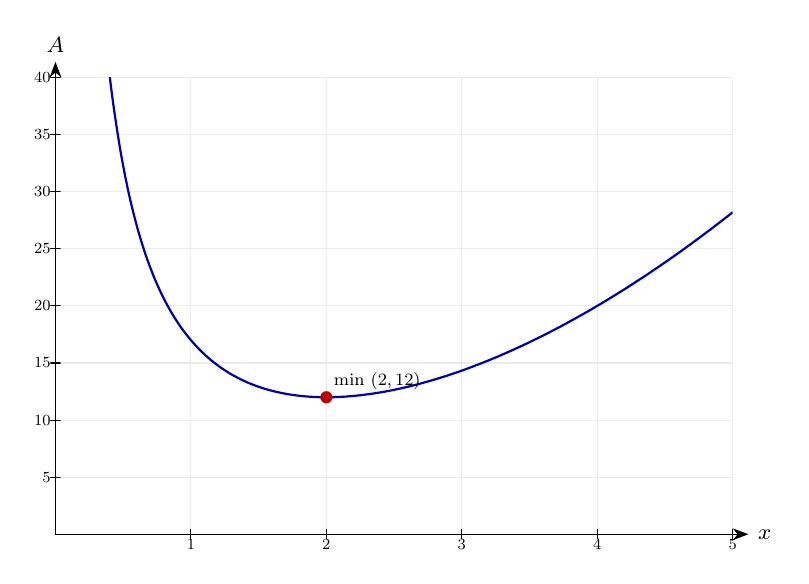
\begin{tikzpicture}[>={Stealth[length=2mm]},font=\footnotesize,line cap=round,line join=round]
\begin{scope}
\clip (0,0) rectangle (8.6,5.8);
\draw[gray!16] (0,0) grid[xstep=1.72,ystep=0.725] (8.6,5.8);
\draw[blue!70!black,thick] (0.031,11.6) -- (0.061,11.6) -- (0.092,11.6) -- (0.123,11.6) -- (0.154,11.6) -- (0.184,11.6) -- (0.215,11.6) -- (0.246,11.6) -- (0.276,11.6) -- (0.307,11.6) -- (0.338,11.6) -- (0.369,10.833) -- (0.399,10.002) -- (0.43,9.289) -- (0.461,8.672) -- (0.491,8.132) -- (0.522,7.656) -- (0.553,7.233) -- (0.584,6.855) -- (0.614,6.514) -- (0.645,6.207) -- (0.676,5.928) -- (0.706,5.673) -- (0.737,5.44) -- (0.768,5.226) -- (0.799,5.028) -- (0.829,4.846) -- (0.86,4.676) -- (0.891,4.519) -- (0.921,4.372) -- (0.952,4.235) -- (0.983,4.107) -- (1.014,3.987) -- (1.044,3.875) -- (1.075,3.769) -- (1.106,3.669) -- (1.136,3.575) -- (1.167,3.486) -- (1.198,3.402) -- (1.229,3.322) -- (1.259,3.247) -- (1.29,3.175) -- (1.321,3.107) -- (1.351,3.042) -- (1.382,2.981) -- (1.413,2.922) -- (1.444,2.866) -- (1.474,2.813) -- (1.505,2.762) -- (1.536,2.714) -- (1.566,2.668) -- (1.597,2.623) -- (1.628,2.581) -- (1.659,2.541) -- (1.689,2.502) -- (1.72,2.465) -- (1.751,2.43) -- (1.781,2.396) -- (1.812,2.363) -- (1.843,2.332) -- (1.874,2.302) -- (1.904,2.273) -- (1.935,2.246) -- (1.966,2.219) -- (1.996,2.194) -- (2.027,2.17) -- (2.058,2.147) -- (2.089,2.124) -- (2.119,2.103) -- (2.15,2.083) -- (2.181,2.063) -- (2.211,2.044) -- (2.242,2.026) -- (2.273,2.009) -- (2.304,1.992) -- (2.334,1.977) -- (2.365,1.961) -- (2.396,1.947) -- (2.426,1.933) -- (2.457,1.92) -- (2.488,1.907) -- (2.519,1.895) -- (2.549,1.884) -- (2.58,1.873) -- (2.611,1.863) -- (2.641,1.853) -- (2.672,1.843) -- (2.703,1.834) -- (2.734,1.826) -- (2.764,1.818) -- (2.795,1.811) -- (2.826,1.804) -- (2.856,1.797) -- (2.887,1.791) -- (2.918,1.785) -- (2.949,1.779) -- (2.979,1.774) -- (3.01,1.77) -- (3.041,1.765) -- (3.071,1.762) -- (3.102,1.758) -- (3.133,1.755) -- (3.164,1.752) -- (3.194,1.749) -- (3.225,1.747) -- (3.256,1.745) -- (3.286,1.744) -- (3.317,1.742) -- (3.348,1.741) -- (3.379,1.741) -- (3.409,1.74) -- (3.44,1.74) -- (3.471,1.74) -- (3.501,1.741) -- (3.532,1.741) -- (3.563,1.742) -- (3.594,1.743) -- (3.624,1.745) -- (3.655,1.747) -- (3.686,1.748) -- (3.716,1.751) -- (3.747,1.753) -- (3.778,1.756) -- (3.809,1.759) -- (3.839,1.762) -- (3.87,1.765) -- (3.901,1.769) -- (3.931,1.773) -- (3.962,1.777) -- (3.993,1.781) -- (4.024,1.785) -- (4.054,1.79) -- (4.085,1.795) -- (4.116,1.8) -- (4.146,1.805) -- (4.177,1.81) -- (4.208,1.816) -- (4.239,1.822) -- (4.269,1.828) -- (4.3,1.834) -- (4.331,1.841) -- (4.361,1.847) -- (4.392,1.854) -- (4.423,1.861) -- (4.454,1.868) -- (4.484,1.875) -- (4.515,1.883) -- (4.546,1.891) -- (4.576,1.898) -- (4.607,1.906) -- (4.638,1.915) -- (4.669,1.923) -- (4.699,1.932) -- (4.73,1.94) -- (4.761,1.949) -- (4.791,1.958) -- (4.822,1.967) -- (4.853,1.977) -- (4.884,1.986) -- (4.914,1.996) -- (4.945,2.005) -- (4.976,2.015) -- (5.006,2.026) -- (5.037,2.036) -- (5.068,2.046) -- (5.099,2.057) -- (5.129,2.067) -- (5.16,2.078) -- (5.191,2.089) -- (5.221,2.1) -- (5.252,2.112) -- (5.283,2.123) -- (5.314,2.135) -- (5.344,2.147) -- (5.375,2.158) -- (5.406,2.17) -- (5.436,2.183) -- (5.467,2.195) -- (5.498,2.207) -- (5.529,2.22) -- (5.559,2.233) -- (5.59,2.245) -- (5.621,2.258) -- (5.651,2.271) -- (5.682,2.285) -- (5.713,2.298) -- (5.744,2.312) -- (5.774,2.325) -- (5.805,2.339) -- (5.836,2.353) -- (5.866,2.367) -- (5.897,2.381) -- (5.928,2.395) -- (5.959,2.41) -- (5.989,2.424) -- (6.02,2.439) -- (6.051,2.454) -- (6.081,2.469) -- (6.112,2.484) -- (6.143,2.499) -- (6.174,2.514) -- (6.204,2.53) -- (6.235,2.545) -- (6.266,2.561) -- (6.296,2.577) -- (6.327,2.593) -- (6.358,2.609) -- (6.389,2.625) -- (6.419,2.641) -- (6.45,2.658) -- (6.481,2.674) -- (6.511,2.691) -- (6.542,2.708) -- (6.573,2.725) -- (6.604,2.742) -- (6.634,2.759) -- (6.665,2.776) -- (6.696,2.793) -- (6.726,2.811) -- (6.757,2.828) -- (6.788,2.846) -- (6.819,2.864) -- (6.849,2.882) -- (6.88,2.9) -- (6.911,2.918) -- (6.941,2.936) -- (6.972,2.955) -- (7.003,2.973) -- (7.034,2.992) -- (7.064,3.011) -- (7.095,3.03) -- (7.126,3.049) -- (7.156,3.068) -- (7.187,3.087) -- (7.218,3.106) -- (7.249,3.126) -- (7.279,3.145) -- (7.31,3.165) -- (7.341,3.185) -- (7.371,3.205) -- (7.402,3.225) -- (7.433,3.245) -- (7.464,3.265) -- (7.494,3.285) -- (7.525,3.306) -- (7.556,3.326) -- (7.586,3.347) -- (7.617,3.368) -- (7.648,3.389) -- (7.679,3.41) -- (7.709,3.431) -- (7.74,3.452) -- (7.771,3.473) -- (7.801,3.495) -- (7.832,3.516) -- (7.863,3.538) -- (7.894,3.559) -- (7.924,3.581) -- (7.955,3.603) -- (7.986,3.625) -- (8.016,3.648) -- (8.047,3.67) -- (8.078,3.692) -- (8.109,3.715) -- (8.139,3.737) -- (8.17,3.76) -- (8.201,3.783) -- (8.231,3.806) -- (8.262,3.829) -- (8.293,3.852) -- (8.324,3.875) -- (8.354,3.898) -- (8.385,3.922) -- (8.416,3.945) -- (8.446,3.969) -- (8.477,3.993) -- (8.508,4.017) -- (8.539,4.041) -- (8.569,4.065) -- (8.6,4.089);
\end{scope}
\draw[->] (0,0) -- (8.8,0) node[right]{$x$};
\draw[->] (0,0) -- (0,6) node[above]{$A$};
\draw (1.72,-0.06) -- (1.72,0.06) node[below=1pt,scale=0.7]{$1$};
\draw (3.44,-0.06) -- (3.44,0.06) node[below=1pt,scale=0.7]{$2$};
\draw (5.16,-0.06) -- (5.16,0.06) node[below=1pt,scale=0.7]{$3$};
\draw (6.88,-0.06) -- (6.88,0.06) node[below=1pt,scale=0.7]{$4$};
\draw (8.6,-0.06) -- (8.6,0.06) node[below=1pt,scale=0.7]{$5$};
\draw (-0.06,0.725) -- (0.06,0.725) node[left=1pt,scale=0.7]{$5$};
\draw (-0.06,1.45) -- (0.06,1.45) node[left=1pt,scale=0.7]{$10$};
\draw (-0.06,2.175) -- (0.06,2.175) node[left=1pt,scale=0.7]{$15$};
\draw (-0.06,2.9) -- (0.06,2.9) node[left=1pt,scale=0.7]{$20$};
\draw (-0.06,3.625) -- (0.06,3.625) node[left=1pt,scale=0.7]{$25$};
\draw (-0.06,4.35) -- (0.06,4.35) node[left=1pt,scale=0.7]{$30$};
\draw (-0.06,5.075) -- (0.06,5.075) node[left=1pt,scale=0.7]{$35$};
\draw (-0.06,5.8) -- (0.06,5.8) node[left=1pt,scale=0.7]{$40$};
\fill[red!75!black] (3.44,1.74) circle (2.2pt);
\node[above right,scale=0.78] at (3.44,1.74) {min $(2,12)$};
\end{tikzpicture}
}
\end{center}
\small The model plotted against its variable, with the key point(s) marked.\normalsize

\medskip\hrule

\section*{Real-Life Problems 36\quad\small\texttt{(d5-036)}}
\addcontentsline{toc}{section}{Real-Life Problems 36 (d5-036)}
\textit{Difficulty: Foundation \quad\textbar\quad Marks: 4}

\question{A particle moves on a straight line with displacement \( s = 2t^3 - 9t^2 + 12t \) metres after \( t \) seconds. (a) Find the velocity \( v \). (b) Find the values of \( t \) at which the particle is instantaneously at rest.}

\textbf{Worked solution.}

\textit{Step 1: (a) Differentiate.}
\[\begin{gathered}
v = \frac{\mathrm{d}s}{\mathrm{d}t} = 6t^2 - 18t + 12
\end{gathered}\]
Velocity is the derivative of displacement. Apply the power rule to each term of \( s \).

\textit{Step 2: (b) Set \( v = 0 \).}
\[\begin{gathered}
6t^2 - 18t + 12 = 0 \implies t^2 - 3t + 2 = 0
\end{gathered}\]
The particle is instantaneously at rest when its velocity is zero. Divide through by 6 to simplify the quadratic.

\textit{Step 3: Factorise.}
\[\begin{gathered}
(t-1)(t-2) = 0 \implies t = 1 \text{ s or } t = 2 \text{ s}
\end{gathered}\]
Two distinct stopping moments --- the particle slows, stops at \( t = 1 \), reverses, then stops again at \( t = 2 \).

\begin{answerbox}
\textbf{Final answer:}\quad (a) \(\displaystyle  v = 6t^2 - 18t + 12 \) \\[3pt]  (b) \(\displaystyle  t = 1 \) s and \(\displaystyle  t = 2 \) s
\end{answerbox}
\textbf{Diagram.}

\begin{center}
\resizebox{\ifdim\width>\linewidth \linewidth\else \width\fi}{!}{%
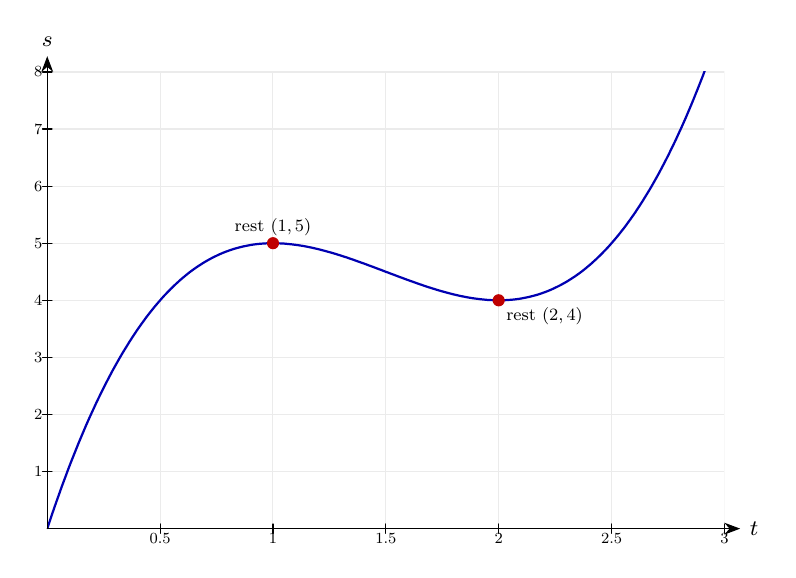
\begin{tikzpicture}[>={Stealth[length=2mm]},font=\footnotesize,line cap=round,line join=round]
\begin{scope}
\clip (0,0) rectangle (8.6,5.8);
\draw[gray!16] (0,0) grid[xstep=1.433,ystep=0.725] (8.6,5.8);
\draw[blue!70!black,thick] (0,0) -- (0.031,0.092) -- (0.061,0.183) -- (0.092,0.273) -- (0.123,0.361) -- (0.154,0.448) -- (0.184,0.533) -- (0.215,0.616) -- (0.246,0.699) -- (0.276,0.78) -- (0.307,0.859) -- (0.338,0.937) -- (0.369,1.014) -- (0.399,1.089) -- (0.43,1.163) -- (0.461,1.236) -- (0.491,1.307) -- (0.522,1.377) -- (0.553,1.446) -- (0.584,1.513) -- (0.614,1.579) -- (0.645,1.644) -- (0.676,1.707) -- (0.706,1.769) -- (0.737,1.83) -- (0.768,1.89) -- (0.799,1.949) -- (0.829,2.006) -- (0.86,2.062) -- (0.891,2.117) -- (0.921,2.17) -- (0.952,2.223) -- (0.983,2.274) -- (1.014,2.324) -- (1.044,2.373) -- (1.075,2.421) -- (1.106,2.468) -- (1.136,2.514) -- (1.167,2.558) -- (1.198,2.602) -- (1.229,2.644) -- (1.259,2.686) -- (1.29,2.726) -- (1.321,2.765) -- (1.351,2.803) -- (1.382,2.84) -- (1.413,2.876) -- (1.444,2.912) -- (1.474,2.946) -- (1.505,2.979) -- (1.536,3.011) -- (1.566,3.042) -- (1.597,3.072) -- (1.628,3.102) -- (1.659,3.13) -- (1.689,3.158) -- (1.72,3.184) -- (1.751,3.21) -- (1.781,3.235) -- (1.812,3.259) -- (1.843,3.282) -- (1.874,3.304) -- (1.904,3.325) -- (1.935,3.345) -- (1.966,3.365) -- (1.996,3.384) -- (2.027,3.402) -- (2.058,3.419) -- (2.089,3.436) -- (2.119,3.451) -- (2.15,3.466) -- (2.181,3.481) -- (2.211,3.494) -- (2.242,3.507) -- (2.273,3.519) -- (2.304,3.53) -- (2.334,3.541) -- (2.365,3.551) -- (2.396,3.56) -- (2.426,3.568) -- (2.457,3.576) -- (2.488,3.584) -- (2.519,3.59) -- (2.549,3.596) -- (2.58,3.602) -- (2.611,3.607) -- (2.641,3.611) -- (2.672,3.615) -- (2.703,3.618) -- (2.734,3.62) -- (2.764,3.622) -- (2.795,3.624) -- (2.826,3.625) -- (2.856,3.625) -- (2.887,3.625) -- (2.918,3.624) -- (2.949,3.623) -- (2.979,3.622) -- (3.01,3.62) -- (3.041,3.617) -- (3.071,3.614) -- (3.102,3.611) -- (3.133,3.607) -- (3.164,3.603) -- (3.194,3.599) -- (3.225,3.594) -- (3.256,3.589) -- (3.286,3.583) -- (3.317,3.577) -- (3.348,3.571) -- (3.379,3.564) -- (3.409,3.557) -- (3.44,3.55) -- (3.471,3.542) -- (3.501,3.534) -- (3.532,3.526) -- (3.563,3.517) -- (3.594,3.509) -- (3.624,3.5) -- (3.655,3.491) -- (3.686,3.481) -- (3.716,3.472) -- (3.747,3.462) -- (3.778,3.452) -- (3.809,3.442) -- (3.839,3.431) -- (3.87,3.421) -- (3.901,3.41) -- (3.931,3.399) -- (3.962,3.388) -- (3.993,3.377) -- (4.024,3.366) -- (4.054,3.355) -- (4.085,3.343) -- (4.116,3.332) -- (4.146,3.321) -- (4.177,3.309) -- (4.208,3.297) -- (4.239,3.286) -- (4.269,3.274) -- (4.3,3.262) -- (4.331,3.251) -- (4.361,3.239) -- (4.392,3.228) -- (4.423,3.216) -- (4.454,3.204) -- (4.484,3.193) -- (4.515,3.182) -- (4.546,3.17) -- (4.576,3.159) -- (4.607,3.148) -- (4.638,3.137) -- (4.669,3.126) -- (4.699,3.115) -- (4.73,3.104) -- (4.761,3.094) -- (4.791,3.083) -- (4.822,3.073) -- (4.853,3.063) -- (4.884,3.053) -- (4.914,3.044) -- (4.945,3.034) -- (4.976,3.025) -- (5.006,3.016) -- (5.037,3.008) -- (5.068,2.999) -- (5.099,2.991) -- (5.129,2.983) -- (5.16,2.975) -- (5.191,2.968) -- (5.221,2.961) -- (5.252,2.954) -- (5.283,2.948) -- (5.314,2.942) -- (5.344,2.936) -- (5.375,2.931) -- (5.406,2.926) -- (5.436,2.922) -- (5.467,2.918) -- (5.498,2.914) -- (5.529,2.911) -- (5.559,2.908) -- (5.59,2.905) -- (5.621,2.903) -- (5.651,2.902) -- (5.682,2.901) -- (5.713,2.9) -- (5.744,2.9) -- (5.774,2.9) -- (5.805,2.901) -- (5.836,2.903) -- (5.866,2.905) -- (5.897,2.907) -- (5.928,2.91) -- (5.959,2.914) -- (5.989,2.918) -- (6.02,2.923) -- (6.051,2.929) -- (6.081,2.935) -- (6.112,2.941) -- (6.143,2.949) -- (6.174,2.957) -- (6.204,2.965) -- (6.235,2.974) -- (6.266,2.984) -- (6.296,2.995) -- (6.327,3.006) -- (6.358,3.018) -- (6.389,3.031) -- (6.419,3.044) -- (6.45,3.059) -- (6.481,3.074) -- (6.511,3.089) -- (6.542,3.106) -- (6.573,3.123) -- (6.604,3.141) -- (6.634,3.16) -- (6.665,3.18) -- (6.696,3.2) -- (6.726,3.221) -- (6.757,3.243) -- (6.788,3.266) -- (6.819,3.29) -- (6.849,3.315) -- (6.88,3.341) -- (6.911,3.367) -- (6.941,3.395) -- (6.972,3.423) -- (7.003,3.453) -- (7.034,3.483) -- (7.064,3.514) -- (7.095,3.546) -- (7.126,3.579) -- (7.156,3.613) -- (7.187,3.649) -- (7.218,3.685) -- (7.249,3.722) -- (7.279,3.76) -- (7.31,3.799) -- (7.341,3.839) -- (7.371,3.881) -- (7.402,3.923) -- (7.433,3.967) -- (7.464,4.011) -- (7.494,4.057) -- (7.525,4.104) -- (7.556,4.152) -- (7.586,4.201) -- (7.617,4.251) -- (7.648,4.302) -- (7.679,4.355) -- (7.709,4.408) -- (7.74,4.463) -- (7.771,4.519) -- (7.801,4.576) -- (7.832,4.635) -- (7.863,4.695) -- (7.894,4.756) -- (7.924,4.818) -- (7.955,4.881) -- (7.986,4.946) -- (8.016,5.012) -- (8.047,5.079) -- (8.078,5.148) -- (8.109,5.218) -- (8.139,5.289) -- (8.17,5.362) -- (8.201,5.436) -- (8.231,5.511) -- (8.262,5.588) -- (8.293,5.666) -- (8.324,5.745) -- (8.354,5.826) -- (8.385,5.909) -- (8.416,5.992) -- (8.446,6.077) -- (8.477,6.164) -- (8.508,6.252) -- (8.539,6.342) -- (8.569,6.433) -- (8.6,6.525);
\end{scope}
\draw[->] (0,0) -- (8.8,0) node[right]{$t$};
\draw[->] (0,0) -- (0,6) node[above]{$s$};
\draw (1.433,-0.06) -- (1.433,0.06) node[below=1pt,scale=0.7]{$0.5$};
\draw (2.867,-0.06) -- (2.867,0.06) node[below=1pt,scale=0.7]{$1$};
\draw (4.3,-0.06) -- (4.3,0.06) node[below=1pt,scale=0.7]{$1.5$};
\draw (5.733,-0.06) -- (5.733,0.06) node[below=1pt,scale=0.7]{$2$};
\draw (7.167,-0.06) -- (7.167,0.06) node[below=1pt,scale=0.7]{$2.5$};
\draw (8.6,-0.06) -- (8.6,0.06) node[below=1pt,scale=0.7]{$3$};
\draw (-0.06,0.725) -- (0.06,0.725) node[left=1pt,scale=0.7]{$1$};
\draw (-0.06,1.45) -- (0.06,1.45) node[left=1pt,scale=0.7]{$2$};
\draw (-0.06,2.175) -- (0.06,2.175) node[left=1pt,scale=0.7]{$3$};
\draw (-0.06,2.9) -- (0.06,2.9) node[left=1pt,scale=0.7]{$4$};
\draw (-0.06,3.625) -- (0.06,3.625) node[left=1pt,scale=0.7]{$5$};
\draw (-0.06,4.35) -- (0.06,4.35) node[left=1pt,scale=0.7]{$6$};
\draw (-0.06,5.075) -- (0.06,5.075) node[left=1pt,scale=0.7]{$7$};
\draw (-0.06,5.8) -- (0.06,5.8) node[left=1pt,scale=0.7]{$8$};
\fill[red!75!black] (2.867,3.625) circle (2.2pt);
\node[above,scale=0.78] at (2.867,3.625) {rest $(1,5)$};
\fill[red!75!black] (5.733,2.9) circle (2.2pt);
\node[below right,scale=0.78] at (5.733,2.9) {rest $(2,4)$};
\end{tikzpicture}
}
\end{center}
\small The model plotted against its variable, with the key point(s) marked.\normalsize

\medskip\hrule

\section*{Real-Life Problems 37\quad\small\texttt{(d5-037)}}
\addcontentsline{toc}{section}{Real-Life Problems 37 (d5-037)}
\textit{Difficulty: Foundation \quad\textbar\quad Marks: 2}

\question{A particle has velocity \( v = 6t^2 - 4t + 1 \) ms\(^{-1}\) at time \( t \) seconds. Find the acceleration when \( t = 3 \).}

\textbf{Worked solution.}

\textit{Step 1: Differentiate to get acceleration.}
\[\begin{gathered}
a = \frac{\mathrm{d}v}{\mathrm{d}t} = 12t - 4
\end{gathered}\]
Acceleration is the rate of change of velocity, so we apply the power rule to \( v = 6t^2 - 4t + 1 \) term by term.

\textit{Step 2: Substitute \( t = 3 \).}
\[\begin{gathered}
a = 12(3) - 4 = 32 \text{ ms}^{-2}
\end{gathered}\]
The units \( \text{ms}^{-2} \) follow because the velocity is in \( \text{ms}^{-1} \) and we differentiated with respect to time in seconds.

\begin{answerbox}
\textbf{Final answer:}\quad \(\displaystyle  a = 32 \text{ ms}^{-2} \)
\end{answerbox}
\textbf{Diagram.}

\begin{center}
\resizebox{\ifdim\width>\linewidth \linewidth\else \width\fi}{!}{%
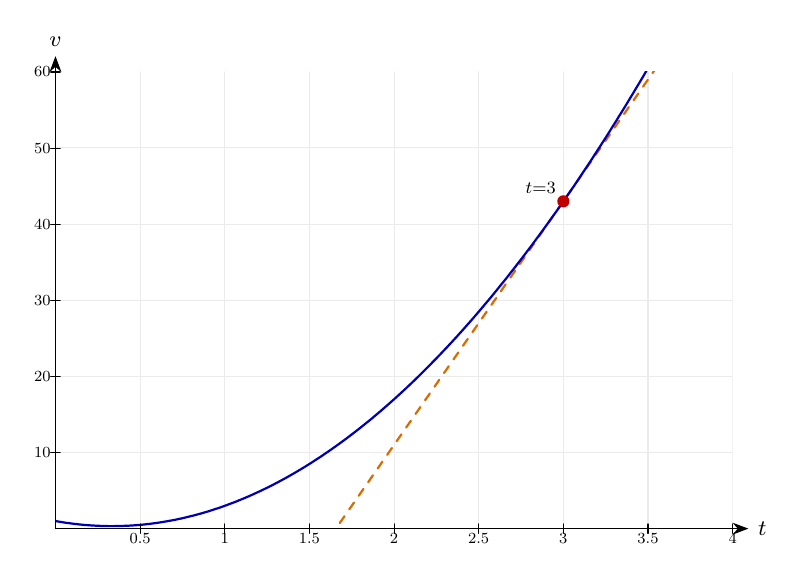
\begin{tikzpicture}[>={Stealth[length=2mm]},font=\footnotesize,line cap=round,line join=round]
\begin{scope}
\clip (0,0) rectangle (8.6,5.8);
\draw[gray!16] (0,0) grid[xstep=1.075,ystep=0.967] (8.6,5.8);
\draw[orange!85!black,thick,dashed] (0,-5.123) -- (8.6,7.25);
\draw[blue!70!black,thick] (0,0.097) -- (0.031,0.091) -- (0.061,0.086) -- (0.092,0.081) -- (0.123,0.076) -- (0.154,0.072) -- (0.184,0.068) -- (0.215,0.064) -- (0.246,0.06) -- (0.276,0.057) -- (0.307,0.053) -- (0.338,0.05) -- (0.369,0.047) -- (0.399,0.045) -- (0.43,0.043) -- (0.461,0.04) -- (0.491,0.039) -- (0.522,0.037) -- (0.553,0.036) -- (0.584,0.034) -- (0.614,0.034) -- (0.645,0.033) -- (0.676,0.032) -- (0.706,0.032) -- (0.737,0.032) -- (0.768,0.033) -- (0.799,0.033) -- (0.829,0.034) -- (0.86,0.035) -- (0.891,0.036) -- (0.921,0.037) -- (0.952,0.039) -- (0.983,0.041) -- (1.014,0.043) -- (1.044,0.046) -- (1.075,0.048) -- (1.106,0.051) -- (1.136,0.054) -- (1.167,0.058) -- (1.198,0.061) -- (1.229,0.065) -- (1.259,0.069) -- (1.29,0.073) -- (1.321,0.078) -- (1.351,0.083) -- (1.382,0.088) -- (1.413,0.093) -- (1.444,0.099) -- (1.474,0.104) -- (1.505,0.11) -- (1.536,0.116) -- (1.566,0.123) -- (1.597,0.129) -- (1.628,0.136) -- (1.659,0.144) -- (1.689,0.151) -- (1.72,0.159) -- (1.751,0.166) -- (1.781,0.174) -- (1.812,0.183) -- (1.843,0.191) -- (1.874,0.2) -- (1.904,0.209) -- (1.935,0.218) -- (1.966,0.228) -- (1.996,0.238) -- (2.027,0.248) -- (2.058,0.258) -- (2.089,0.268) -- (2.119,0.279) -- (2.15,0.29) -- (2.181,0.301) -- (2.211,0.313) -- (2.242,0.324) -- (2.273,0.336) -- (2.304,0.348) -- (2.334,0.361) -- (2.365,0.373) -- (2.396,0.386) -- (2.426,0.399) -- (2.457,0.412) -- (2.488,0.426) -- (2.519,0.44) -- (2.549,0.454) -- (2.58,0.468) -- (2.611,0.482) -- (2.641,0.497) -- (2.672,0.512) -- (2.703,0.527) -- (2.734,0.543) -- (2.764,0.558) -- (2.795,0.574) -- (2.826,0.59) -- (2.856,0.607) -- (2.887,0.623) -- (2.918,0.64) -- (2.949,0.657) -- (2.979,0.675) -- (3.01,0.692) -- (3.041,0.71) -- (3.071,0.728) -- (3.102,0.746) -- (3.133,0.765) -- (3.164,0.783) -- (3.194,0.802) -- (3.225,0.822) -- (3.256,0.841) -- (3.286,0.861) -- (3.317,0.881) -- (3.348,0.901) -- (3.379,0.921) -- (3.409,0.942) -- (3.44,0.963) -- (3.471,0.984) -- (3.501,1.005) -- (3.532,1.027) -- (3.563,1.049) -- (3.594,1.071) -- (3.624,1.093) -- (3.655,1.116) -- (3.686,1.138) -- (3.716,1.161) -- (3.747,1.185) -- (3.778,1.208) -- (3.809,1.232) -- (3.839,1.256) -- (3.87,1.28) -- (3.901,1.304) -- (3.931,1.329) -- (3.962,1.354) -- (3.993,1.379) -- (4.024,1.404) -- (4.054,1.43) -- (4.085,1.456) -- (4.116,1.482) -- (4.146,1.508) -- (4.177,1.535) -- (4.208,1.562) -- (4.239,1.589) -- (4.269,1.616) -- (4.3,1.643) -- (4.331,1.671) -- (4.361,1.699) -- (4.392,1.727) -- (4.423,1.756) -- (4.454,1.784) -- (4.484,1.813) -- (4.515,1.842) -- (4.546,1.872) -- (4.576,1.901) -- (4.607,1.931) -- (4.638,1.961) -- (4.669,1.992) -- (4.699,2.022) -- (4.73,2.053) -- (4.761,2.084) -- (4.791,2.116) -- (4.822,2.147) -- (4.853,2.179) -- (4.884,2.211) -- (4.914,2.243) -- (4.945,2.276) -- (4.976,2.308) -- (5.006,2.341) -- (5.037,2.374) -- (5.068,2.408) -- (5.099,2.441) -- (5.129,2.475) -- (5.16,2.509) -- (5.191,2.544) -- (5.221,2.578) -- (5.252,2.613) -- (5.283,2.648) -- (5.314,2.684) -- (5.344,2.719) -- (5.375,2.755) -- (5.406,2.791) -- (5.436,2.827) -- (5.467,2.864) -- (5.498,2.901) -- (5.529,2.937) -- (5.559,2.975) -- (5.59,3.012) -- (5.621,3.05) -- (5.651,3.088) -- (5.682,3.126) -- (5.713,3.164) -- (5.744,3.203) -- (5.774,3.242) -- (5.805,3.281) -- (5.836,3.32) -- (5.866,3.36) -- (5.897,3.4) -- (5.928,3.44) -- (5.959,3.48) -- (5.989,3.52) -- (6.02,3.561) -- (6.051,3.602) -- (6.081,3.643) -- (6.112,3.685) -- (6.143,3.727) -- (6.174,3.769) -- (6.204,3.811) -- (6.235,3.853) -- (6.266,3.896) -- (6.296,3.939) -- (6.327,3.982) -- (6.358,4.025) -- (6.389,4.069) -- (6.419,4.113) -- (6.45,4.157) -- (6.481,4.201) -- (6.511,4.246) -- (6.542,4.29) -- (6.573,4.335) -- (6.604,4.381) -- (6.634,4.426) -- (6.665,4.472) -- (6.696,4.518) -- (6.726,4.564) -- (6.757,4.61) -- (6.788,4.657) -- (6.819,4.704) -- (6.849,4.751) -- (6.88,4.799) -- (6.911,4.846) -- (6.941,4.894) -- (6.972,4.942) -- (7.003,4.99) -- (7.034,5.039) -- (7.064,5.088) -- (7.095,5.137) -- (7.126,5.186) -- (7.156,5.236) -- (7.187,5.285) -- (7.218,5.335) -- (7.249,5.386) -- (7.279,5.436) -- (7.31,5.487) -- (7.341,5.538) -- (7.371,5.589) -- (7.402,5.64) -- (7.433,5.692) -- (7.464,5.744) -- (7.494,5.796) -- (7.525,5.848) -- (7.556,5.901) -- (7.586,5.954) -- (7.617,6.007) -- (7.648,6.06) -- (7.679,6.114) -- (7.709,6.167) -- (7.74,6.221) -- (7.771,6.276) -- (7.801,6.33) -- (7.832,6.385) -- (7.863,6.44) -- (7.894,6.495) -- (7.924,6.551) -- (7.955,6.606) -- (7.986,6.662) -- (8.016,6.718) -- (8.047,6.775) -- (8.078,6.831) -- (8.109,6.888) -- (8.139,6.945) -- (8.17,7.003) -- (8.201,7.06) -- (8.231,7.118) -- (8.262,7.176) -- (8.293,7.234) -- (8.324,7.293) -- (8.354,7.351) -- (8.385,7.41) -- (8.416,7.47) -- (8.446,7.529) -- (8.477,7.589) -- (8.508,7.649) -- (8.539,7.709) -- (8.569,7.769) -- (8.6,7.83);
\end{scope}
\draw[->] (0,0) -- (8.8,0) node[right]{$t$};
\draw[->] (0,0) -- (0,6) node[above]{$v$};
\draw (1.075,-0.06) -- (1.075,0.06) node[below=1pt,scale=0.7]{$0.5$};
\draw (2.15,-0.06) -- (2.15,0.06) node[below=1pt,scale=0.7]{$1$};
\draw (3.225,-0.06) -- (3.225,0.06) node[below=1pt,scale=0.7]{$1.5$};
\draw (4.3,-0.06) -- (4.3,0.06) node[below=1pt,scale=0.7]{$2$};
\draw (5.375,-0.06) -- (5.375,0.06) node[below=1pt,scale=0.7]{$2.5$};
\draw (6.45,-0.06) -- (6.45,0.06) node[below=1pt,scale=0.7]{$3$};
\draw (7.525,-0.06) -- (7.525,0.06) node[below=1pt,scale=0.7]{$3.5$};
\draw (8.6,-0.06) -- (8.6,0.06) node[below=1pt,scale=0.7]{$4$};
\draw (-0.06,0.967) -- (0.06,0.967) node[left=1pt,scale=0.7]{$10$};
\draw (-0.06,1.933) -- (0.06,1.933) node[left=1pt,scale=0.7]{$20$};
\draw (-0.06,2.9) -- (0.06,2.9) node[left=1pt,scale=0.7]{$30$};
\draw (-0.06,3.867) -- (0.06,3.867) node[left=1pt,scale=0.7]{$40$};
\draw (-0.06,4.833) -- (0.06,4.833) node[left=1pt,scale=0.7]{$50$};
\draw (-0.06,5.8) -- (0.06,5.8) node[left=1pt,scale=0.7]{$60$};
\fill[red!75!black] (6.45,4.157) circle (2.2pt);
\node[above left,scale=0.78] at (6.45,4.157) {$t{=}3$};
\end{tikzpicture}
}
\end{center}
\small The model plotted against its variable, with the key point(s) marked and the tangent (dashed) showing the instantaneous rate.\normalsize

\medskip\hrule

\section*{Real-Life Problems 38\quad\small\texttt{(d5-038)}}
\addcontentsline{toc}{section}{Real-Life Problems 38 (d5-038)}
\textit{Difficulty: Standard \quad\textbar\quad Marks: 6}

\question{An open box is made by cutting equal squares of side \( x \) cm from the corners of a square sheet of card of side 12 cm and folding up the sides. The volume is \( V = x(12 - 2x)^2 \) cm\(^3\). (a) Find \( \dfrac{\mathrm{d}V}{\mathrm{d}x} \). (b) Find the value of \( x \) that maximises \( V \) and the maximum volume.}

\textbf{Worked solution.}

\textit{Step 1: Expand.}
\[\begin{gathered}
V = x(144 - 48x + 4x^2) = 144x - 48x^2 + 4x^3
\end{gathered}\]
Expand \( (12 - 2x)^2 \) first, then multiply by \( x \). Expanding into a polynomial makes term-by-term differentiation straightforward.

\textit{Step 2: (a) Differentiate.}
\[\begin{gathered}
\frac{\mathrm{d}V}{\mathrm{d}x} = 144 - 96x + 12x^2
\end{gathered}\]
Apply the power rule to each term.

\textit{Step 3: (b) Set to zero.}
\[\begin{gathered}
12x^2 - 96x + 144 = 0 \implies x^2 - 8x + 12 = 0
\end{gathered}\]
Setting \( \dfrac{\mathrm{d}V}{\mathrm{d}x} = 0 \) locates the stationary points of \( V \), where the volume is neither increasing nor decreasing. Divide through by 12 to simplify.

\textit{Step 4: Factorise.}
\[\begin{gathered}
(x-2)(x-6) = 0 \implies x = 2 \text{ (since } x = 6 \text{ gives } V = 0)
\end{gathered}\]
The root \( x = 6 \) makes the base side \( 12 - 2x = 0 \), giving a degenerate "box" of zero volume --- reject it as it cannot be a maximum.

\textit{Step 5: Maximum volume.}
\[\begin{gathered}
V = 2(12 - 4)^2 = 2 \cdot 64 = 128 \text{ cm}^3
\end{gathered}\]
Substitute \( x = 2 \) back into the original volume expression. (You could also check \( \dfrac{\mathrm{d}^2V}{\mathrm{d}x^2} = -96 + 24x \), giving \( -48 < 0 \) at \( x = 2 \), confirming a maximum.)

\begin{answerbox}
\textbf{Final answer:}\quad (a) \(\displaystyle  144 - 96x + 12x^2 \) \\[3pt]  (b) \(\displaystyle  x = 2 \) cm; \(\displaystyle  V_{\max} = 128 \text{ cm}^3 \)
\end{answerbox}
\textbf{Diagram.}

\begin{center}
\resizebox{\ifdim\width>\linewidth \linewidth\else \width\fi}{!}{%
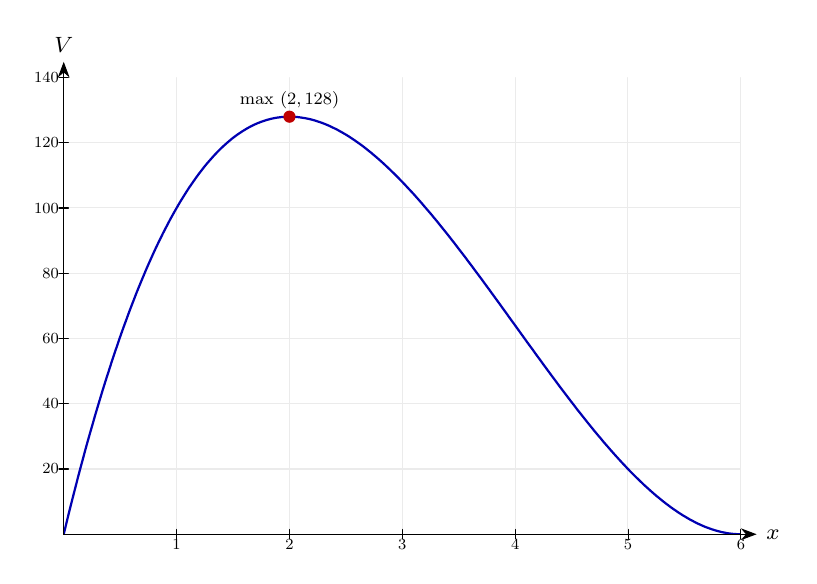
\begin{tikzpicture}[>={Stealth[length=2mm]},font=\footnotesize,line cap=round,line join=round]
\begin{scope}
\clip (0,0) rectangle (8.6,5.8);
\draw[gray!16] (0,0) grid[xstep=1.433,ystep=0.829] (8.6,5.8);
\draw[blue!70!black,thick] (0,0) -- (0.031,0.127) -- (0.061,0.252) -- (0.092,0.375) -- (0.123,0.497) -- (0.154,0.617) -- (0.184,0.735) -- (0.215,0.851) -- (0.246,0.965) -- (0.276,1.078) -- (0.307,1.189) -- (0.338,1.298) -- (0.369,1.405) -- (0.399,1.511) -- (0.43,1.615) -- (0.461,1.718) -- (0.491,1.818) -- (0.522,1.917) -- (0.553,2.015) -- (0.584,2.11) -- (0.614,2.205) -- (0.645,2.297) -- (0.676,2.388) -- (0.706,2.477) -- (0.737,2.565) -- (0.768,2.651) -- (0.799,2.735) -- (0.829,2.818) -- (0.86,2.899) -- (0.891,2.979) -- (0.921,3.057) -- (0.952,3.134) -- (0.983,3.209) -- (1.014,3.283) -- (1.044,3.355) -- (1.075,3.426) -- (1.106,3.495) -- (1.136,3.562) -- (1.167,3.629) -- (1.198,3.694) -- (1.229,3.757) -- (1.259,3.819) -- (1.29,3.879) -- (1.321,3.938) -- (1.351,3.996) -- (1.382,4.052) -- (1.413,4.107) -- (1.444,4.161) -- (1.474,4.213) -- (1.505,4.263) -- (1.536,4.313) -- (1.566,4.361) -- (1.597,4.408) -- (1.628,4.453) -- (1.659,4.497) -- (1.689,4.54) -- (1.72,4.582) -- (1.751,4.622) -- (1.781,4.661) -- (1.812,4.699) -- (1.843,4.735) -- (1.874,4.77) -- (1.904,4.804) -- (1.935,4.837) -- (1.966,4.869) -- (1.996,4.899) -- (2.027,4.928) -- (2.058,4.956) -- (2.089,4.983) -- (2.119,5.009) -- (2.15,5.034) -- (2.181,5.057) -- (2.211,5.079) -- (2.242,5.1) -- (2.273,5.12) -- (2.304,5.139) -- (2.334,5.157) -- (2.365,5.174) -- (2.396,5.19) -- (2.426,5.204) -- (2.457,5.218) -- (2.488,5.23) -- (2.519,5.242) -- (2.549,5.252) -- (2.58,5.262) -- (2.611,5.27) -- (2.641,5.278) -- (2.672,5.284) -- (2.703,5.29) -- (2.734,5.294) -- (2.764,5.298) -- (2.795,5.3) -- (2.826,5.302) -- (2.856,5.303) -- (2.887,5.303) -- (2.918,5.302) -- (2.949,5.3) -- (2.979,5.297) -- (3.01,5.293) -- (3.041,5.288) -- (3.071,5.283) -- (3.102,5.277) -- (3.133,5.27) -- (3.164,5.262) -- (3.194,5.253) -- (3.225,5.243) -- (3.256,5.233) -- (3.286,5.222) -- (3.317,5.21) -- (3.348,5.197) -- (3.379,5.184) -- (3.409,5.169) -- (3.44,5.154) -- (3.471,5.139) -- (3.501,5.122) -- (3.532,5.105) -- (3.563,5.087) -- (3.594,5.069) -- (3.624,5.05) -- (3.655,5.03) -- (3.686,5.009) -- (3.716,4.988) -- (3.747,4.966) -- (3.778,4.944) -- (3.809,4.921) -- (3.839,4.897) -- (3.87,4.872) -- (3.901,4.848) -- (3.931,4.822) -- (3.962,4.796) -- (3.993,4.769) -- (4.024,4.742) -- (4.054,4.715) -- (4.085,4.686) -- (4.116,4.657) -- (4.146,4.628) -- (4.177,4.598) -- (4.208,4.568) -- (4.239,4.537) -- (4.269,4.506) -- (4.3,4.474) -- (4.331,4.442) -- (4.361,4.409) -- (4.392,4.376) -- (4.423,4.343) -- (4.454,4.309) -- (4.484,4.275) -- (4.515,4.24) -- (4.546,4.205) -- (4.576,4.169) -- (4.607,4.133) -- (4.638,4.097) -- (4.669,4.061) -- (4.699,4.024) -- (4.73,3.987) -- (4.761,3.949) -- (4.791,3.911) -- (4.822,3.873) -- (4.853,3.835) -- (4.884,3.796) -- (4.914,3.757) -- (4.945,3.718) -- (4.976,3.678) -- (5.006,3.638) -- (5.037,3.598) -- (5.068,3.558) -- (5.099,3.518) -- (5.129,3.477) -- (5.16,3.436) -- (5.191,3.395) -- (5.221,3.354) -- (5.252,3.313) -- (5.283,3.271) -- (5.314,3.23) -- (5.344,3.188) -- (5.375,3.146) -- (5.406,3.104) -- (5.436,3.062) -- (5.467,3.02) -- (5.498,2.977) -- (5.529,2.935) -- (5.559,2.893) -- (5.59,2.85) -- (5.621,2.808) -- (5.651,2.765) -- (5.682,2.722) -- (5.713,2.68) -- (5.744,2.637) -- (5.774,2.595) -- (5.805,2.552) -- (5.836,2.509) -- (5.866,2.467) -- (5.897,2.424) -- (5.928,2.382) -- (5.959,2.34) -- (5.989,2.297) -- (6.02,2.255) -- (6.051,2.213) -- (6.081,2.171) -- (6.112,2.129) -- (6.143,2.087) -- (6.174,2.045) -- (6.204,2.004) -- (6.235,1.963) -- (6.266,1.921) -- (6.296,1.88) -- (6.327,1.839) -- (6.358,1.799) -- (6.389,1.758) -- (6.419,1.718) -- (6.45,1.678) -- (6.481,1.638) -- (6.511,1.598) -- (6.542,1.559) -- (6.573,1.52) -- (6.604,1.481) -- (6.634,1.443) -- (6.665,1.404) -- (6.696,1.366) -- (6.726,1.329) -- (6.757,1.291) -- (6.788,1.254) -- (6.819,1.218) -- (6.849,1.181) -- (6.88,1.145) -- (6.911,1.11) -- (6.941,1.075) -- (6.972,1.04) -- (7.003,1.005) -- (7.034,0.971) -- (7.064,0.938) -- (7.095,0.904) -- (7.126,0.872) -- (7.156,0.839) -- (7.187,0.807) -- (7.218,0.776) -- (7.249,0.745) -- (7.279,0.715) -- (7.31,0.685) -- (7.341,0.655) -- (7.371,0.626) -- (7.402,0.598) -- (7.433,0.57) -- (7.464,0.542) -- (7.494,0.516) -- (7.525,0.489) -- (7.556,0.464) -- (7.586,0.439) -- (7.617,0.414) -- (7.648,0.39) -- (7.679,0.367) -- (7.709,0.344) -- (7.74,0.322) -- (7.771,0.301) -- (7.801,0.28) -- (7.832,0.26) -- (7.863,0.24) -- (7.894,0.222) -- (7.924,0.204) -- (7.955,0.186) -- (7.986,0.17) -- (8.016,0.154) -- (8.047,0.138) -- (8.078,0.124) -- (8.109,0.11) -- (8.139,0.097) -- (8.17,0.085) -- (8.201,0.074) -- (8.231,0.063) -- (8.262,0.053) -- (8.293,0.044) -- (8.324,0.036) -- (8.354,0.028) -- (8.385,0.022) -- (8.416,0.016) -- (8.446,0.011) -- (8.477,0.007) -- (8.508,0.004) -- (8.539,0.002) -- (8.569,0) -- (8.6,0);
\end{scope}
\draw[->] (0,0) -- (8.8,0) node[right]{$x$};
\draw[->] (0,0) -- (0,6) node[above]{$V$};
\draw (1.433,-0.06) -- (1.433,0.06) node[below=1pt,scale=0.7]{$1$};
\draw (2.867,-0.06) -- (2.867,0.06) node[below=1pt,scale=0.7]{$2$};
\draw (4.3,-0.06) -- (4.3,0.06) node[below=1pt,scale=0.7]{$3$};
\draw (5.733,-0.06) -- (5.733,0.06) node[below=1pt,scale=0.7]{$4$};
\draw (7.167,-0.06) -- (7.167,0.06) node[below=1pt,scale=0.7]{$5$};
\draw (8.6,-0.06) -- (8.6,0.06) node[below=1pt,scale=0.7]{$6$};
\draw (-0.06,0.829) -- (0.06,0.829) node[left=1pt,scale=0.7]{$20$};
\draw (-0.06,1.657) -- (0.06,1.657) node[left=1pt,scale=0.7]{$40$};
\draw (-0.06,2.486) -- (0.06,2.486) node[left=1pt,scale=0.7]{$60$};
\draw (-0.06,3.314) -- (0.06,3.314) node[left=1pt,scale=0.7]{$80$};
\draw (-0.06,4.143) -- (0.06,4.143) node[left=1pt,scale=0.7]{$100$};
\draw (-0.06,4.971) -- (0.06,4.971) node[left=1pt,scale=0.7]{$120$};
\draw (-0.06,5.8) -- (0.06,5.8) node[left=1pt,scale=0.7]{$140$};
\fill[red!75!black] (2.867,5.303) circle (2.2pt);
\node[above,scale=0.78] at (2.867,5.303) {max $(2,128)$};
\end{tikzpicture}
}
\end{center}
\small The model plotted against its variable, with the key point(s) marked.\normalsize

\medskip\hrule

\section*{Real-Life Problems 39\quad\small\texttt{(d5-039)}}
\addcontentsline{toc}{section}{Real-Life Problems 39 (d5-039)}
\textit{Difficulty: Foundation \quad\textbar\quad Marks: 4}

\question{A small business has profit \( P = -2x^2 + 80x - 200 \) pounds when \( x \) units are sold per day. Find the value of \( x \) that maximises profit and the maximum profit.}

\textbf{Worked solution.}

\textit{Step 1: Differentiate.}
\[\begin{gathered}
\frac{\mathrm{d}P}{\mathrm{d}x} = -4x + 80
\end{gathered}\]
This is the marginal profit --- the extra profit per additional unit sold.

\textit{Step 2: Set to zero.}
\[\begin{gathered}
-4x + 80 = 0 \implies x = 20
\end{gathered}\]
At the maximum, marginal profit is zero --- one more unit adds nothing. The negative coefficient of \( x^2 \) means \( P \) is a downward parabola, so this stationary point is guaranteed to be a maximum.

\textit{Step 3: Maximum profit.}
\[\begin{gathered}
P = -2(400) + 80(20) - 200 = -800 + 1600 - 200 = 600
\end{gathered}\]
Substitute \( x = 20 \) back into the original profit function.

\begin{answerbox}
\textbf{Final answer:}\quad \(\displaystyle  x = 20 \); maximum profit \(\displaystyle  = \pounds 600 \)
\end{answerbox}
\textbf{Diagram.}

\begin{center}
\resizebox{\ifdim\width>\linewidth \linewidth\else \width\fi}{!}{%
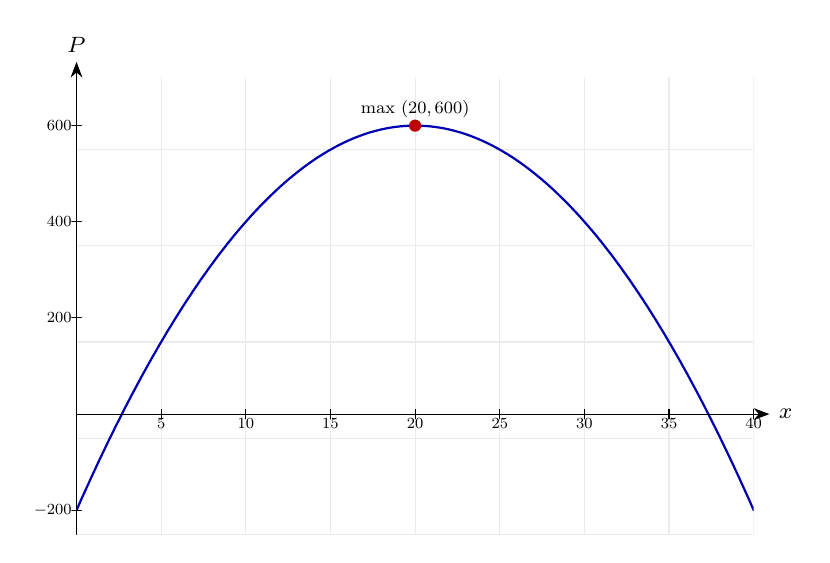
\begin{tikzpicture}[>={Stealth[length=2mm]},font=\footnotesize,line cap=round,line join=round]
\begin{scope}
\clip (0,0) rectangle (8.6,5.8);
\draw[gray!16] (0,-0.916) grid[xstep=1.075,ystep=1.221] (8.6,5.8);
\draw[blue!70!black,thick] (0,0.305) -- (0.031,0.375) -- (0.061,0.444) -- (0.092,0.512) -- (0.123,0.58) -- (0.154,0.648) -- (0.184,0.715) -- (0.215,0.781) -- (0.246,0.848) -- (0.276,0.913) -- (0.307,0.978) -- (0.338,1.043) -- (0.369,1.107) -- (0.399,1.17) -- (0.43,1.233) -- (0.461,1.296) -- (0.491,1.358) -- (0.522,1.419) -- (0.553,1.48) -- (0.584,1.541) -- (0.614,1.601) -- (0.645,1.661) -- (0.676,1.72) -- (0.706,1.778) -- (0.737,1.836) -- (0.768,1.894) -- (0.799,1.951) -- (0.829,2.008) -- (0.86,2.064) -- (0.891,2.119) -- (0.921,2.174) -- (0.952,2.229) -- (0.983,2.283) -- (1.014,2.336) -- (1.044,2.39) -- (1.075,2.442) -- (1.106,2.494) -- (1.136,2.546) -- (1.167,2.597) -- (1.198,2.647) -- (1.229,2.698) -- (1.259,2.747) -- (1.29,2.796) -- (1.321,2.845) -- (1.351,2.893) -- (1.382,2.94) -- (1.413,2.988) -- (1.444,3.034) -- (1.474,3.08) -- (1.505,3.126) -- (1.536,3.171) -- (1.566,3.216) -- (1.597,3.26) -- (1.628,3.303) -- (1.659,3.346) -- (1.689,3.389) -- (1.72,3.431) -- (1.751,3.473) -- (1.781,3.514) -- (1.812,3.555) -- (1.843,3.595) -- (1.874,3.634) -- (1.904,3.673) -- (1.935,3.712) -- (1.966,3.75) -- (1.996,3.788) -- (2.027,3.825) -- (2.058,3.862) -- (2.089,3.898) -- (2.119,3.933) -- (2.15,3.968) -- (2.181,4.003) -- (2.211,4.037) -- (2.242,4.071) -- (2.273,4.104) -- (2.304,4.137) -- (2.334,4.169) -- (2.365,4.2) -- (2.396,4.232) -- (2.426,4.262) -- (2.457,4.292) -- (2.488,4.322) -- (2.519,4.351) -- (2.549,4.38) -- (2.58,4.408) -- (2.611,4.436) -- (2.641,4.463) -- (2.672,4.489) -- (2.703,4.516) -- (2.734,4.541) -- (2.764,4.566) -- (2.795,4.591) -- (2.826,4.615) -- (2.856,4.639) -- (2.887,4.662) -- (2.918,4.685) -- (2.949,4.707) -- (2.979,4.729) -- (3.01,4.75) -- (3.041,4.771) -- (3.071,4.791) -- (3.102,4.81) -- (3.133,4.83) -- (3.164,4.848) -- (3.194,4.867) -- (3.225,4.884) -- (3.256,4.901) -- (3.286,4.918) -- (3.317,4.934) -- (3.348,4.95) -- (3.379,4.965) -- (3.409,4.98) -- (3.44,4.994) -- (3.471,5.008) -- (3.501,5.021) -- (3.532,5.034) -- (3.563,5.046) -- (3.594,5.058) -- (3.624,5.069) -- (3.655,5.08) -- (3.686,5.09) -- (3.716,5.1) -- (3.747,5.109) -- (3.778,5.117) -- (3.809,5.126) -- (3.839,5.133) -- (3.87,5.141) -- (3.901,5.147) -- (3.931,5.154) -- (3.962,5.159) -- (3.993,5.165) -- (4.024,5.169) -- (4.054,5.174) -- (4.085,5.177) -- (4.116,5.181) -- (4.146,5.183) -- (4.177,5.185) -- (4.208,5.187) -- (4.239,5.188) -- (4.269,5.189) -- (4.3,5.189) -- (4.331,5.189) -- (4.361,5.188) -- (4.392,5.187) -- (4.423,5.185) -- (4.454,5.183) -- (4.484,5.181) -- (4.515,5.177) -- (4.546,5.174) -- (4.576,5.169) -- (4.607,5.165) -- (4.638,5.159) -- (4.669,5.154) -- (4.699,5.147) -- (4.73,5.141) -- (4.761,5.133) -- (4.791,5.126) -- (4.822,5.117) -- (4.853,5.109) -- (4.884,5.1) -- (4.914,5.09) -- (4.945,5.08) -- (4.976,5.069) -- (5.006,5.058) -- (5.037,5.046) -- (5.068,5.034) -- (5.099,5.021) -- (5.129,5.008) -- (5.16,4.994) -- (5.191,4.98) -- (5.221,4.965) -- (5.252,4.95) -- (5.283,4.934) -- (5.314,4.918) -- (5.344,4.901) -- (5.375,4.884) -- (5.406,4.867) -- (5.436,4.848) -- (5.467,4.83) -- (5.498,4.81) -- (5.529,4.791) -- (5.559,4.771) -- (5.59,4.75) -- (5.621,4.729) -- (5.651,4.707) -- (5.682,4.685) -- (5.713,4.662) -- (5.744,4.639) -- (5.774,4.615) -- (5.805,4.591) -- (5.836,4.566) -- (5.866,4.541) -- (5.897,4.516) -- (5.928,4.489) -- (5.959,4.463) -- (5.989,4.436) -- (6.02,4.408) -- (6.051,4.38) -- (6.081,4.351) -- (6.112,4.322) -- (6.143,4.292) -- (6.174,4.262) -- (6.204,4.232) -- (6.235,4.2) -- (6.266,4.169) -- (6.296,4.137) -- (6.327,4.104) -- (6.358,4.071) -- (6.389,4.037) -- (6.419,4.003) -- (6.45,3.968) -- (6.481,3.933) -- (6.511,3.898) -- (6.542,3.862) -- (6.573,3.825) -- (6.604,3.788) -- (6.634,3.75) -- (6.665,3.712) -- (6.696,3.673) -- (6.726,3.634) -- (6.757,3.595) -- (6.788,3.555) -- (6.819,3.514) -- (6.849,3.473) -- (6.88,3.431) -- (6.911,3.389) -- (6.941,3.346) -- (6.972,3.303) -- (7.003,3.26) -- (7.034,3.216) -- (7.064,3.171) -- (7.095,3.126) -- (7.126,3.08) -- (7.156,3.034) -- (7.187,2.988) -- (7.218,2.94) -- (7.249,2.893) -- (7.279,2.845) -- (7.31,2.796) -- (7.341,2.747) -- (7.371,2.698) -- (7.402,2.647) -- (7.433,2.597) -- (7.464,2.546) -- (7.494,2.494) -- (7.525,2.442) -- (7.556,2.39) -- (7.586,2.336) -- (7.617,2.283) -- (7.648,2.229) -- (7.679,2.174) -- (7.709,2.119) -- (7.74,2.064) -- (7.771,2.008) -- (7.801,1.951) -- (7.832,1.894) -- (7.863,1.836) -- (7.894,1.778) -- (7.924,1.72) -- (7.955,1.661) -- (7.986,1.601) -- (8.016,1.541) -- (8.047,1.48) -- (8.078,1.419) -- (8.109,1.358) -- (8.139,1.296) -- (8.17,1.233) -- (8.201,1.17) -- (8.231,1.107) -- (8.262,1.043) -- (8.293,0.978) -- (8.324,0.913) -- (8.354,0.848) -- (8.385,0.781) -- (8.416,0.715) -- (8.446,0.648) -- (8.477,0.58) -- (8.508,0.512) -- (8.539,0.444) -- (8.569,0.375) -- (8.6,0.305);
\end{scope}
\draw[->] (0,1.526) -- (8.8,1.526) node[right]{$x$};
\draw[->] (0,0) -- (0,6) node[above]{$P$};
\draw (1.075,1.466) -- (1.075,1.586) node[below=1pt,scale=0.7]{$5$};
\draw (2.15,1.466) -- (2.15,1.586) node[below=1pt,scale=0.7]{$10$};
\draw (3.225,1.466) -- (3.225,1.586) node[below=1pt,scale=0.7]{$15$};
\draw (4.3,1.466) -- (4.3,1.586) node[below=1pt,scale=0.7]{$20$};
\draw (5.375,1.466) -- (5.375,1.586) node[below=1pt,scale=0.7]{$25$};
\draw (6.45,1.466) -- (6.45,1.586) node[below=1pt,scale=0.7]{$30$};
\draw (7.525,1.466) -- (7.525,1.586) node[below=1pt,scale=0.7]{$35$};
\draw (8.6,1.466) -- (8.6,1.586) node[below=1pt,scale=0.7]{$40$};
\draw (-0.06,0.305) -- (0.06,0.305) node[left=1pt,scale=0.7]{$-200$};
\draw (-0.06,2.747) -- (0.06,2.747) node[left=1pt,scale=0.7]{$200$};
\draw (-0.06,3.968) -- (0.06,3.968) node[left=1pt,scale=0.7]{$400$};
\draw (-0.06,5.189) -- (0.06,5.189) node[left=1pt,scale=0.7]{$600$};
\fill[red!75!black] (4.3,5.189) circle (2.2pt);
\node[above,scale=0.78] at (4.3,5.189) {max $(20,600)$};
\end{tikzpicture}
}
\end{center}
\small The model plotted against its variable, with the key point(s) marked.\normalsize

\medskip\hrule

\section*{Real-Life Problems 40\quad\small\texttt{(d5-040)}}
\addcontentsline{toc}{section}{Real-Life Problems 40 (d5-040)}
\textit{Difficulty: Foundation \quad\textbar\quad Marks: 5}

\question{A rectangle has perimeter 40 m. Find the dimensions that give the maximum area, and state the maximum area.}

\textbf{Worked solution.}

\textit{Step 1: Let sides be \( x \) and \( y \).}
\[\begin{gathered}
2x + 2y = 40 \implies y = 20 - x
\end{gathered}\]
Use the perimeter constraint to express \( y \) in terms of \( x \) --- this reduces the area from two variables to one.

\textit{Step 2: Area as a function of \( x \).}
\[\begin{gathered}
A = x(20 - x) = 20x - x^2
\end{gathered}\]
Substitute \( y = 20 - x \) into \( A = xy \). Now \( A \) depends on a single variable, ready for calculus.

\textit{Step 3: Differentiate.}
\[\begin{gathered}
\frac{\mathrm{d}A}{\mathrm{d}x} = 20 - 2x = 0 \implies x = 10
\end{gathered}\]
Setting the derivative to zero finds the stationary point of \( A \). Since \( A = 20x - x^2 \) is a downward parabola, this stationary point is the maximum.

\textit{Step 4: Maximum area.}
\[\begin{gathered}
A = 10 \cdot 10 = 100 \text{ m}^2
\end{gathered}\]
A square of side 10 m --- for a fixed perimeter, the square always gives the greatest rectangular area.

\begin{answerbox}
\textbf{Final answer:}\quad \(\displaystyle  10 \text{ m} \times 10 \text{ m} \); area \(\displaystyle  = 100 \text{ m}^2 \)
\end{answerbox}
\textbf{Diagram.}

\begin{center}
\resizebox{\ifdim\width>\linewidth \linewidth\else \width\fi}{!}{%
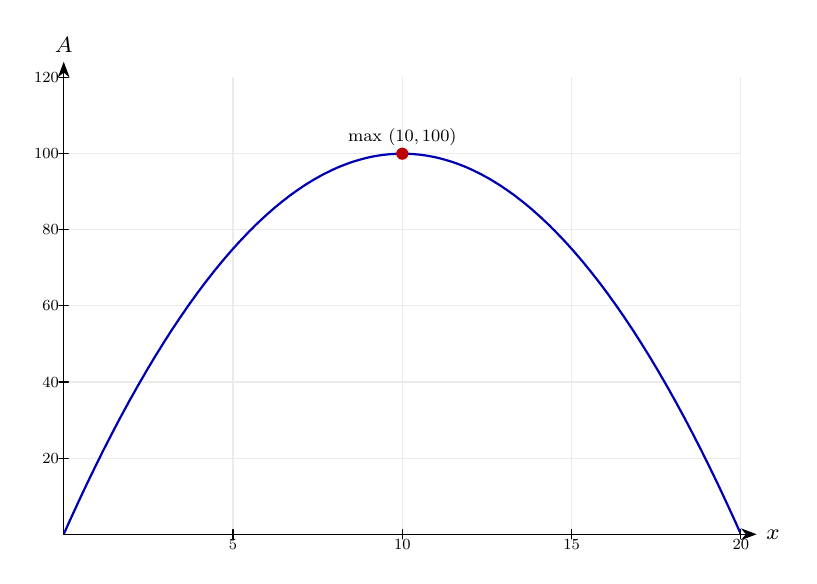
\begin{tikzpicture}[>={Stealth[length=2mm]},font=\footnotesize,line cap=round,line join=round]
\begin{scope}
\clip (0,0) rectangle (8.6,5.8);
\draw[gray!16] (0,0) grid[xstep=2.15,ystep=0.967] (8.6,5.8);
\draw[blue!70!black,thick] (0,0) -- (0.031,0.069) -- (0.061,0.137) -- (0.092,0.205) -- (0.123,0.272) -- (0.154,0.339) -- (0.184,0.405) -- (0.215,0.471) -- (0.246,0.537) -- (0.276,0.601) -- (0.307,0.666) -- (0.338,0.73) -- (0.369,0.793) -- (0.399,0.856) -- (0.43,0.918) -- (0.461,0.98) -- (0.491,1.042) -- (0.522,1.103) -- (0.553,1.163) -- (0.584,1.223) -- (0.614,1.282) -- (0.645,1.341) -- (0.676,1.4) -- (0.706,1.458) -- (0.737,1.515) -- (0.768,1.572) -- (0.799,1.629) -- (0.829,1.685) -- (0.86,1.74) -- (0.891,1.795) -- (0.921,1.849) -- (0.952,1.903) -- (0.983,1.957) -- (1.014,2.01) -- (1.044,2.063) -- (1.075,2.115) -- (1.106,2.166) -- (1.136,2.217) -- (1.167,2.268) -- (1.198,2.318) -- (1.229,2.367) -- (1.259,2.416) -- (1.29,2.465) -- (1.321,2.513) -- (1.351,2.561) -- (1.382,2.608) -- (1.413,2.654) -- (1.444,2.701) -- (1.474,2.746) -- (1.505,2.791) -- (1.536,2.836) -- (1.566,2.88) -- (1.597,2.924) -- (1.628,2.967) -- (1.659,3.009) -- (1.689,3.052) -- (1.72,3.093) -- (1.751,3.135) -- (1.781,3.175) -- (1.812,3.215) -- (1.843,3.255) -- (1.874,3.294) -- (1.904,3.333) -- (1.935,3.371) -- (1.966,3.409) -- (1.996,3.446) -- (2.027,3.483) -- (2.058,3.519) -- (2.089,3.555) -- (2.119,3.59) -- (2.15,3.625) -- (2.181,3.659) -- (2.211,3.693) -- (2.242,3.726) -- (2.273,3.759) -- (2.304,3.791) -- (2.334,3.823) -- (2.365,3.855) -- (2.396,3.885) -- (2.426,3.916) -- (2.457,3.946) -- (2.488,3.975) -- (2.519,4.004) -- (2.549,4.032) -- (2.58,4.06) -- (2.611,4.087) -- (2.641,4.114) -- (2.672,4.141) -- (2.703,4.167) -- (2.734,4.192) -- (2.764,4.217) -- (2.795,4.241) -- (2.826,4.265) -- (2.856,4.289) -- (2.887,4.312) -- (2.918,4.334) -- (2.949,4.356) -- (2.979,4.377) -- (3.01,4.398) -- (3.041,4.419) -- (3.071,4.439) -- (3.102,4.458) -- (3.133,4.477) -- (3.164,4.496) -- (3.194,4.514) -- (3.225,4.531) -- (3.256,4.548) -- (3.286,4.565) -- (3.317,4.581) -- (3.348,4.596) -- (3.379,4.611) -- (3.409,4.626) -- (3.44,4.64) -- (3.471,4.654) -- (3.501,4.667) -- (3.532,4.679) -- (3.563,4.691) -- (3.594,4.703) -- (3.624,4.714) -- (3.655,4.725) -- (3.686,4.735) -- (3.716,4.744) -- (3.747,4.753) -- (3.778,4.762) -- (3.809,4.77) -- (3.839,4.778) -- (3.87,4.785) -- (3.901,4.792) -- (3.931,4.798) -- (3.962,4.803) -- (3.993,4.809) -- (4.024,4.813) -- (4.054,4.818) -- (4.085,4.821) -- (4.116,4.824) -- (4.146,4.827) -- (4.177,4.829) -- (4.208,4.831) -- (4.239,4.832) -- (4.269,4.833) -- (4.3,4.833) -- (4.331,4.833) -- (4.361,4.832) -- (4.392,4.831) -- (4.423,4.829) -- (4.454,4.827) -- (4.484,4.824) -- (4.515,4.821) -- (4.546,4.818) -- (4.576,4.813) -- (4.607,4.809) -- (4.638,4.803) -- (4.669,4.798) -- (4.699,4.792) -- (4.73,4.785) -- (4.761,4.778) -- (4.791,4.77) -- (4.822,4.762) -- (4.853,4.753) -- (4.884,4.744) -- (4.914,4.735) -- (4.945,4.725) -- (4.976,4.714) -- (5.006,4.703) -- (5.037,4.691) -- (5.068,4.679) -- (5.099,4.667) -- (5.129,4.654) -- (5.16,4.64) -- (5.191,4.626) -- (5.221,4.611) -- (5.252,4.596) -- (5.283,4.581) -- (5.314,4.565) -- (5.344,4.548) -- (5.375,4.531) -- (5.406,4.514) -- (5.436,4.496) -- (5.467,4.477) -- (5.498,4.458) -- (5.529,4.439) -- (5.559,4.419) -- (5.59,4.398) -- (5.621,4.377) -- (5.651,4.356) -- (5.682,4.334) -- (5.713,4.312) -- (5.744,4.289) -- (5.774,4.265) -- (5.805,4.241) -- (5.836,4.217) -- (5.866,4.192) -- (5.897,4.167) -- (5.928,4.141) -- (5.959,4.114) -- (5.989,4.087) -- (6.02,4.06) -- (6.051,4.032) -- (6.081,4.004) -- (6.112,3.975) -- (6.143,3.946) -- (6.174,3.916) -- (6.204,3.885) -- (6.235,3.855) -- (6.266,3.823) -- (6.296,3.791) -- (6.327,3.759) -- (6.358,3.726) -- (6.389,3.693) -- (6.419,3.659) -- (6.45,3.625) -- (6.481,3.59) -- (6.511,3.555) -- (6.542,3.519) -- (6.573,3.483) -- (6.604,3.446) -- (6.634,3.409) -- (6.665,3.371) -- (6.696,3.333) -- (6.726,3.294) -- (6.757,3.255) -- (6.788,3.215) -- (6.819,3.175) -- (6.849,3.135) -- (6.88,3.093) -- (6.911,3.052) -- (6.941,3.009) -- (6.972,2.967) -- (7.003,2.924) -- (7.034,2.88) -- (7.064,2.836) -- (7.095,2.791) -- (7.126,2.746) -- (7.156,2.701) -- (7.187,2.654) -- (7.218,2.608) -- (7.249,2.561) -- (7.279,2.513) -- (7.31,2.465) -- (7.341,2.416) -- (7.371,2.367) -- (7.402,2.318) -- (7.433,2.268) -- (7.464,2.217) -- (7.494,2.166) -- (7.525,2.115) -- (7.556,2.063) -- (7.586,2.01) -- (7.617,1.957) -- (7.648,1.903) -- (7.679,1.849) -- (7.709,1.795) -- (7.74,1.74) -- (7.771,1.685) -- (7.801,1.629) -- (7.832,1.572) -- (7.863,1.515) -- (7.894,1.458) -- (7.924,1.4) -- (7.955,1.341) -- (7.986,1.282) -- (8.016,1.223) -- (8.047,1.163) -- (8.078,1.103) -- (8.109,1.042) -- (8.139,0.98) -- (8.17,0.918) -- (8.201,0.856) -- (8.231,0.793) -- (8.262,0.73) -- (8.293,0.666) -- (8.324,0.601) -- (8.354,0.537) -- (8.385,0.471) -- (8.416,0.405) -- (8.446,0.339) -- (8.477,0.272) -- (8.508,0.205) -- (8.539,0.137) -- (8.569,0.069) -- (8.6,0);
\end{scope}
\draw[->] (0,0) -- (8.8,0) node[right]{$x$};
\draw[->] (0,0) -- (0,6) node[above]{$A$};
\draw (2.15,-0.06) -- (2.15,0.06) node[below=1pt,scale=0.7]{$5$};
\draw (4.3,-0.06) -- (4.3,0.06) node[below=1pt,scale=0.7]{$10$};
\draw (6.45,-0.06) -- (6.45,0.06) node[below=1pt,scale=0.7]{$15$};
\draw (8.6,-0.06) -- (8.6,0.06) node[below=1pt,scale=0.7]{$20$};
\draw (-0.06,0.967) -- (0.06,0.967) node[left=1pt,scale=0.7]{$20$};
\draw (-0.06,1.933) -- (0.06,1.933) node[left=1pt,scale=0.7]{$40$};
\draw (-0.06,2.9) -- (0.06,2.9) node[left=1pt,scale=0.7]{$60$};
\draw (-0.06,3.867) -- (0.06,3.867) node[left=1pt,scale=0.7]{$80$};
\draw (-0.06,4.833) -- (0.06,4.833) node[left=1pt,scale=0.7]{$100$};
\draw (-0.06,5.8) -- (0.06,5.8) node[left=1pt,scale=0.7]{$120$};
\fill[red!75!black] (4.3,4.833) circle (2.2pt);
\node[above,scale=0.78] at (4.3,4.833) {max $(10,100)$};
\end{tikzpicture}
}
\end{center}
\small The model plotted against its variable, with the key point(s) marked.\normalsize

\medskip\hrule

\section*{Real-Life Problems 41\quad\small\texttt{(d5-041)}}
\addcontentsline{toc}{section}{Real-Life Problems 41 (d5-041)}
\textit{Difficulty: Standard \quad\textbar\quad Marks: 7}

\question{A closed cylindrical can has volume \( 16\pi \) cm\(^3\). Find the radius and height that minimise the total surface area, and state the minimum surface area.}

\textbf{Worked solution.}

\textit{Step 1: Volume constraint.}
\[\begin{gathered}
\pi r^2 h = 16\pi \implies h = \frac{16}{r^2}
\end{gathered}\]
The fixed-volume condition links \( h \) to \( r \). Use it to eliminate \( h \) from the surface area so we have a function of \( r \) alone.

\textit{Step 2: Total surface area.}
\[\begin{gathered}
A = 2\pi r^2 + 2\pi r h = 2\pi r^2 + \frac{32\pi}{r}
\end{gathered}\]
Two circular ends contribute \( 2\pi r^2 \); the curved side contributes \( 2\pi r h \). Substituting \( h = 16/r^2 \) gives a single-variable expression.

\textit{Step 3: Differentiate.}
\[\begin{gathered}
\frac{\mathrm{d}A}{\mathrm{d}r} = 4\pi r - \frac{32\pi}{r^2}
\end{gathered}\]
Rewriting \( \dfrac{32\pi}{r} \) as \( 32\pi r^{-1} \) gives derivative \( -32\pi r^{-2} \). Power rule.

\textit{Step 4: Set to zero.}
\[\begin{gathered}
4\pi r = \frac{32\pi}{r^2} \implies r^3 = 8 \implies r = 2
\end{gathered}\]
At the optimal radius the marginal surface-area change is zero. Multiply both sides by \( r^2 \) and divide by \( 4\pi \) to isolate \( r^3 \).

\textit{Step 5: Find \( h \) and \( A \).}
\[\begin{gathered}
h = \frac{16}{4} = 4; \quad A = 8\pi + 16\pi = 24\pi \text{ cm}^2
\end{gathered}\]
Substitute \( r = 2 \) back into the constraint to find \( h \), then into \( A \). Notice \( h = 2r \): for a closed cylinder of fixed volume, minimum surface area occurs when height equals diameter.

\textit{Step 6: Confirm minimum.}
\[\begin{gathered}
\frac{\mathrm{d}^2A}{\mathrm{d}r^2} = 4\pi + \frac{64\pi}{r^3} > 0 \Rightarrow \text{min} \checkmark
\end{gathered}\]
Both terms are positive for \( r > 0 \), so the second derivative is positive everywhere --- guaranteeing the stationary point is a minimum.

\begin{answerbox}
\textbf{Final answer:}\quad \(\displaystyle  r = 2 \) cm, \(\displaystyle  h = 4 \) cm, \(\displaystyle  A_{\min} = 24\pi \text{ cm}^2 \)
\end{answerbox}
\textbf{Diagram.}

\begin{center}
\resizebox{\ifdim\width>\linewidth \linewidth\else \width\fi}{!}{%
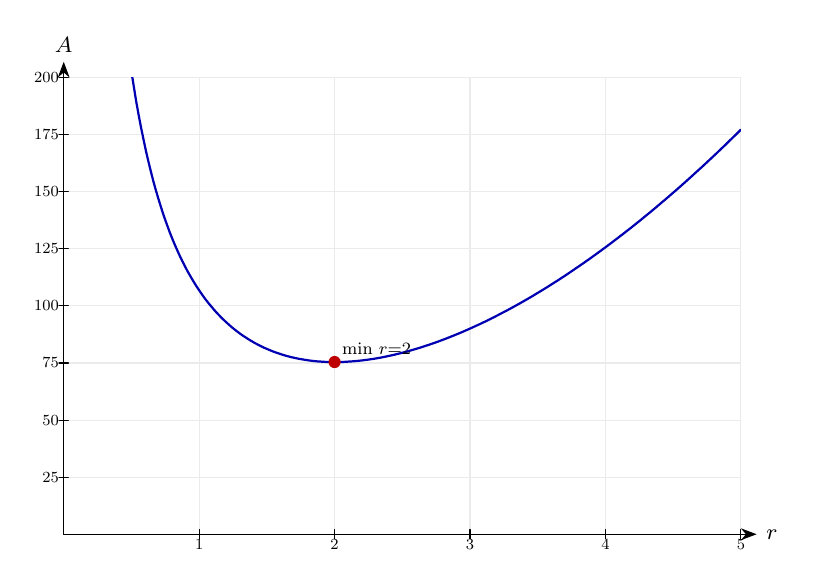
\begin{tikzpicture}[>={Stealth[length=2mm]},font=\footnotesize,line cap=round,line join=round]
\begin{scope}
\clip (0,0) rectangle (8.6,5.8);
\draw[gray!16] (0,0) grid[xstep=1.72,ystep=0.725] (8.6,5.8);
\draw[blue!70!black,thick] (0.031,11.6) -- (0.061,11.6) -- (0.092,11.6) -- (0.123,11.6) -- (0.154,11.6) -- (0.184,11.6) -- (0.215,11.6) -- (0.246,11.6) -- (0.276,11.6) -- (0.307,11.6) -- (0.338,11.6) -- (0.369,11.6) -- (0.399,11.6) -- (0.43,11.6) -- (0.461,10.897) -- (0.491,10.219) -- (0.522,9.62) -- (0.553,9.089) -- (0.584,8.614) -- (0.614,8.186) -- (0.645,7.8) -- (0.676,7.449) -- (0.706,7.129) -- (0.737,6.836) -- (0.768,6.567) -- (0.799,6.319) -- (0.829,6.089) -- (0.86,5.876) -- (0.891,5.679) -- (0.921,5.494) -- (0.952,5.322) -- (0.983,5.161) -- (1.014,5.011) -- (1.044,4.869) -- (1.075,4.736) -- (1.106,4.61) -- (1.136,4.492) -- (1.167,4.38) -- (1.198,4.275) -- (1.229,4.175) -- (1.259,4.08) -- (1.29,3.99) -- (1.321,3.904) -- (1.351,3.823) -- (1.382,3.746) -- (1.413,3.672) -- (1.444,3.602) -- (1.474,3.535) -- (1.505,3.471) -- (1.536,3.411) -- (1.566,3.352) -- (1.597,3.297) -- (1.628,3.244) -- (1.659,3.193) -- (1.689,3.144) -- (1.72,3.098) -- (1.751,3.053) -- (1.781,3.01) -- (1.812,2.969) -- (1.843,2.93) -- (1.874,2.893) -- (1.904,2.857) -- (1.935,2.822) -- (1.966,2.789) -- (1.996,2.757) -- (2.027,2.727) -- (2.058,2.698) -- (2.089,2.67) -- (2.119,2.643) -- (2.15,2.617) -- (2.181,2.592) -- (2.211,2.569) -- (2.242,2.546) -- (2.273,2.524) -- (2.304,2.504) -- (2.334,2.484) -- (2.365,2.465) -- (2.396,2.447) -- (2.426,2.429) -- (2.457,2.413) -- (2.488,2.397) -- (2.519,2.382) -- (2.549,2.367) -- (2.58,2.354) -- (2.611,2.341) -- (2.641,2.328) -- (2.672,2.316) -- (2.703,2.305) -- (2.734,2.295) -- (2.764,2.285) -- (2.795,2.275) -- (2.826,2.266) -- (2.856,2.258) -- (2.887,2.25) -- (2.918,2.243) -- (2.949,2.236) -- (2.979,2.23) -- (3.01,2.224) -- (3.041,2.219) -- (3.071,2.214) -- (3.102,2.209) -- (3.133,2.205) -- (3.164,2.201) -- (3.194,2.198) -- (3.225,2.195) -- (3.256,2.193) -- (3.286,2.191) -- (3.317,2.189) -- (3.348,2.188) -- (3.379,2.187) -- (3.409,2.187) -- (3.44,2.187) -- (3.471,2.187) -- (3.501,2.187) -- (3.532,2.188) -- (3.563,2.189) -- (3.594,2.191) -- (3.624,2.193) -- (3.655,2.195) -- (3.686,2.197) -- (3.716,2.2) -- (3.747,2.203) -- (3.778,2.206) -- (3.809,2.21) -- (3.839,2.214) -- (3.87,2.218) -- (3.901,2.223) -- (3.931,2.227) -- (3.962,2.232) -- (3.993,2.238) -- (4.024,2.243) -- (4.054,2.249) -- (4.085,2.255) -- (4.116,2.262) -- (4.146,2.268) -- (4.177,2.275) -- (4.208,2.282) -- (4.239,2.29) -- (4.269,2.297) -- (4.3,2.305) -- (4.331,2.313) -- (4.361,2.321) -- (4.392,2.33) -- (4.423,2.339) -- (4.454,2.348) -- (4.484,2.357) -- (4.515,2.366) -- (4.546,2.376) -- (4.576,2.386) -- (4.607,2.396) -- (4.638,2.406) -- (4.669,2.417) -- (4.699,2.427) -- (4.73,2.438) -- (4.761,2.449) -- (4.791,2.461) -- (4.822,2.472) -- (4.853,2.484) -- (4.884,2.496) -- (4.914,2.508) -- (4.945,2.52) -- (4.976,2.533) -- (5.006,2.545) -- (5.037,2.558) -- (5.068,2.571) -- (5.099,2.585) -- (5.129,2.598) -- (5.16,2.612) -- (5.191,2.626) -- (5.221,2.64) -- (5.252,2.654) -- (5.283,2.668) -- (5.314,2.683) -- (5.344,2.697) -- (5.375,2.712) -- (5.406,2.727) -- (5.436,2.743) -- (5.467,2.758) -- (5.498,2.774) -- (5.529,2.79) -- (5.559,2.806) -- (5.59,2.822) -- (5.621,2.838) -- (5.651,2.854) -- (5.682,2.871) -- (5.713,2.888) -- (5.744,2.905) -- (5.774,2.922) -- (5.805,2.939) -- (5.836,2.957) -- (5.866,2.974) -- (5.897,2.992) -- (5.928,3.01) -- (5.959,3.028) -- (5.989,3.047) -- (6.02,3.065) -- (6.051,3.084) -- (6.081,3.102) -- (6.112,3.121) -- (6.143,3.14) -- (6.174,3.16) -- (6.204,3.179) -- (6.235,3.199) -- (6.266,3.218) -- (6.296,3.238) -- (6.327,3.258) -- (6.358,3.278) -- (6.389,3.299) -- (6.419,3.319) -- (6.45,3.34) -- (6.481,3.361) -- (6.511,3.382) -- (6.542,3.403) -- (6.573,3.424) -- (6.604,3.445) -- (6.634,3.467) -- (6.665,3.488) -- (6.696,3.51) -- (6.726,3.532) -- (6.757,3.554) -- (6.788,3.577) -- (6.819,3.599) -- (6.849,3.622) -- (6.88,3.644) -- (6.911,3.667) -- (6.941,3.69) -- (6.972,3.713) -- (7.003,3.737) -- (7.034,3.76) -- (7.064,3.784) -- (7.095,3.807) -- (7.126,3.831) -- (7.156,3.855) -- (7.187,3.879) -- (7.218,3.903) -- (7.249,3.928) -- (7.279,3.952) -- (7.31,3.977) -- (7.341,4.002) -- (7.371,4.027) -- (7.402,4.052) -- (7.433,4.077) -- (7.464,4.103) -- (7.494,4.128) -- (7.525,4.154) -- (7.556,4.18) -- (7.586,4.206) -- (7.617,4.232) -- (7.648,4.258) -- (7.679,4.285) -- (7.709,4.311) -- (7.74,4.338) -- (7.771,4.364) -- (7.801,4.391) -- (7.832,4.418) -- (7.863,4.446) -- (7.894,4.473) -- (7.924,4.5) -- (7.955,4.528) -- (7.986,4.556) -- (8.016,4.584) -- (8.047,4.612) -- (8.078,4.64) -- (8.109,4.668) -- (8.139,4.696) -- (8.17,4.725) -- (8.201,4.754) -- (8.231,4.782) -- (8.262,4.811) -- (8.293,4.84) -- (8.324,4.87) -- (8.354,4.899) -- (8.385,4.928) -- (8.416,4.958) -- (8.446,4.988) -- (8.477,5.018) -- (8.508,5.048) -- (8.539,5.078) -- (8.569,5.108) -- (8.6,5.138);
\end{scope}
\draw[->] (0,0) -- (8.8,0) node[right]{$r$};
\draw[->] (0,0) -- (0,6) node[above]{$A$};
\draw (1.72,-0.06) -- (1.72,0.06) node[below=1pt,scale=0.7]{$1$};
\draw (3.44,-0.06) -- (3.44,0.06) node[below=1pt,scale=0.7]{$2$};
\draw (5.16,-0.06) -- (5.16,0.06) node[below=1pt,scale=0.7]{$3$};
\draw (6.88,-0.06) -- (6.88,0.06) node[below=1pt,scale=0.7]{$4$};
\draw (8.6,-0.06) -- (8.6,0.06) node[below=1pt,scale=0.7]{$5$};
\draw (-0.06,0.725) -- (0.06,0.725) node[left=1pt,scale=0.7]{$25$};
\draw (-0.06,1.45) -- (0.06,1.45) node[left=1pt,scale=0.7]{$50$};
\draw (-0.06,2.175) -- (0.06,2.175) node[left=1pt,scale=0.7]{$75$};
\draw (-0.06,2.9) -- (0.06,2.9) node[left=1pt,scale=0.7]{$100$};
\draw (-0.06,3.625) -- (0.06,3.625) node[left=1pt,scale=0.7]{$125$};
\draw (-0.06,4.35) -- (0.06,4.35) node[left=1pt,scale=0.7]{$150$};
\draw (-0.06,5.075) -- (0.06,5.075) node[left=1pt,scale=0.7]{$175$};
\draw (-0.06,5.8) -- (0.06,5.8) node[left=1pt,scale=0.7]{$200$};
\fill[red!75!black] (3.44,2.187) circle (2.2pt);
\node[above right,scale=0.78] at (3.44,2.187) {min $r{=}2$};
\end{tikzpicture}
}
\end{center}
\small The model plotted against its variable, with the key point(s) marked.\normalsize

\medskip\hrule

\section*{Real-Life Problems 42\quad\small\texttt{(d5-042)}}
\addcontentsline{toc}{section}{Real-Life Problems 42 (d5-042)}
\textit{Difficulty: Foundation \quad\textbar\quad Marks: 4}

\question{A population of insects is modelled by \( P = 50t - t^2 \) (in thousands) for \( 0 \le t \le 50 \) days. Find the day on which the population is greatest and the maximum population.}

\textbf{Worked solution.}

\textit{Step 1: Differentiate.}
\[\begin{gathered}
\frac{\mathrm{d}P}{\mathrm{d}t} = 50 - 2t
\end{gathered}\]
\( \dfrac{\mathrm{d}P}{\mathrm{d}t} \) gives the daily rate of change of the population.

\textit{Step 2: Set to zero.}
\[\begin{gathered}
50 - 2t = 0 \implies t = 25
\end{gathered}\]
The population peaks when its rate of change is zero --- before this, population is growing; after, it is declining. \( t = 25 \) lies inside the allowed window \( 0 \le t \le 50 \).

\textit{Step 3: Maximum population.}
\[\begin{gathered}
P = 50(25) - 25^2 = 1250 - 625 = 625 \text{ thousand}
\end{gathered}\]
Substitute \( t = 25 \) back into \( P \). Since the coefficient of \( t^2 \) is negative, the curve is a downward parabola, so this stationary point is indeed the maximum.

\begin{answerbox}
\textbf{Final answer:}\quad Day \(\displaystyle  t = 25 \); maximum \(\displaystyle  P = 625{,}000 \) insects
\end{answerbox}
\textbf{Diagram.}

\begin{center}
\resizebox{\ifdim\width>\linewidth \linewidth\else \width\fi}{!}{%
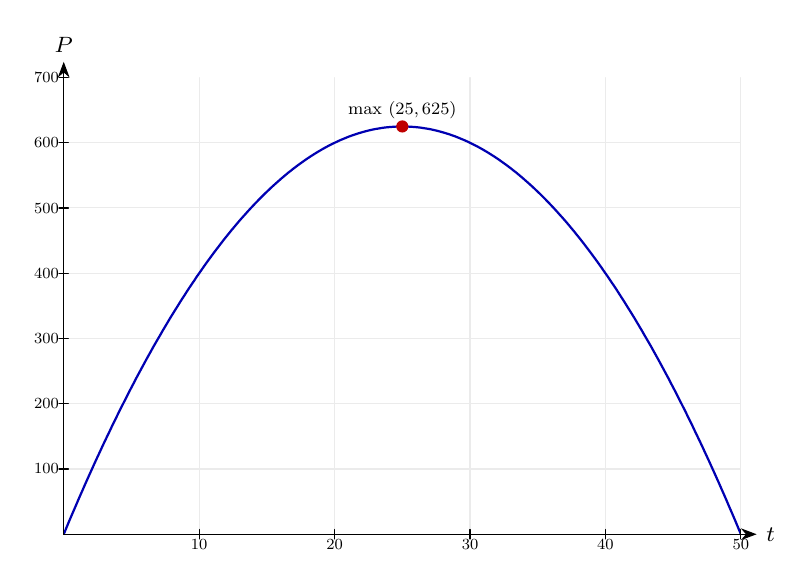
\begin{tikzpicture}[>={Stealth[length=2mm]},font=\footnotesize,line cap=round,line join=round]
\begin{scope}
\clip (0,0) rectangle (8.6,5.8);
\draw[gray!16] (0,0) grid[xstep=1.72,ystep=0.829] (8.6,5.8);
\draw[blue!70!black,thick] (0,0) -- (0.031,0.074) -- (0.061,0.147) -- (0.092,0.22) -- (0.123,0.292) -- (0.154,0.363) -- (0.184,0.434) -- (0.215,0.505) -- (0.246,0.575) -- (0.276,0.644) -- (0.307,0.713) -- (0.338,0.782) -- (0.369,0.85) -- (0.399,0.917) -- (0.43,0.984) -- (0.461,1.05) -- (0.491,1.116) -- (0.522,1.181) -- (0.553,1.246) -- (0.584,1.31) -- (0.614,1.374) -- (0.645,1.437) -- (0.676,1.5) -- (0.706,1.562) -- (0.737,1.623) -- (0.768,1.684) -- (0.799,1.745) -- (0.829,1.805) -- (0.86,1.864) -- (0.891,1.923) -- (0.921,1.982) -- (0.952,2.039) -- (0.983,2.097) -- (1.014,2.154) -- (1.044,2.21) -- (1.075,2.266) -- (1.106,2.321) -- (1.136,2.376) -- (1.167,2.43) -- (1.198,2.483) -- (1.229,2.536) -- (1.259,2.589) -- (1.29,2.641) -- (1.321,2.693) -- (1.351,2.744) -- (1.382,2.794) -- (1.413,2.844) -- (1.444,2.893) -- (1.474,2.942) -- (1.505,2.991) -- (1.536,3.038) -- (1.566,3.086) -- (1.597,3.133) -- (1.628,3.179) -- (1.659,3.224) -- (1.689,3.27) -- (1.72,3.314) -- (1.751,3.358) -- (1.781,3.402) -- (1.812,3.445) -- (1.843,3.488) -- (1.874,3.53) -- (1.904,3.571) -- (1.935,3.612) -- (1.966,3.652) -- (1.996,3.692) -- (2.027,3.732) -- (2.058,3.771) -- (2.089,3.809) -- (2.119,3.847) -- (2.15,3.884) -- (2.181,3.921) -- (2.211,3.957) -- (2.242,3.993) -- (2.273,4.028) -- (2.304,4.062) -- (2.334,4.096) -- (2.365,4.13) -- (2.396,4.163) -- (2.426,4.195) -- (2.457,4.227) -- (2.488,4.259) -- (2.519,4.29) -- (2.549,4.32) -- (2.58,4.35) -- (2.611,4.379) -- (2.641,4.408) -- (2.672,4.436) -- (2.703,4.464) -- (2.734,4.491) -- (2.764,4.518) -- (2.795,4.544) -- (2.826,4.57) -- (2.856,4.595) -- (2.887,4.619) -- (2.918,4.644) -- (2.949,4.667) -- (2.979,4.69) -- (3.01,4.712) -- (3.041,4.734) -- (3.071,4.756) -- (3.102,4.777) -- (3.133,4.797) -- (3.164,4.817) -- (3.194,4.836) -- (3.225,4.855) -- (3.256,4.873) -- (3.286,4.891) -- (3.317,4.908) -- (3.348,4.925) -- (3.379,4.941) -- (3.409,4.956) -- (3.44,4.971) -- (3.471,4.986) -- (3.501,5) -- (3.532,5.013) -- (3.563,5.026) -- (3.594,5.039) -- (3.624,5.051) -- (3.655,5.062) -- (3.686,5.073) -- (3.716,5.083) -- (3.747,5.093) -- (3.778,5.102) -- (3.809,5.111) -- (3.839,5.119) -- (3.87,5.127) -- (3.901,5.134) -- (3.931,5.141) -- (3.962,5.147) -- (3.993,5.152) -- (4.024,5.157) -- (4.054,5.162) -- (4.085,5.166) -- (4.116,5.169) -- (4.146,5.172) -- (4.177,5.174) -- (4.208,5.176) -- (4.239,5.178) -- (4.269,5.178) -- (4.3,5.179) -- (4.331,5.178) -- (4.361,5.178) -- (4.392,5.176) -- (4.423,5.174) -- (4.454,5.172) -- (4.484,5.169) -- (4.515,5.166) -- (4.546,5.162) -- (4.576,5.157) -- (4.607,5.152) -- (4.638,5.147) -- (4.669,5.141) -- (4.699,5.134) -- (4.73,5.127) -- (4.761,5.119) -- (4.791,5.111) -- (4.822,5.102) -- (4.853,5.093) -- (4.884,5.083) -- (4.914,5.073) -- (4.945,5.062) -- (4.976,5.051) -- (5.006,5.039) -- (5.037,5.026) -- (5.068,5.013) -- (5.099,5) -- (5.129,4.986) -- (5.16,4.971) -- (5.191,4.956) -- (5.221,4.941) -- (5.252,4.925) -- (5.283,4.908) -- (5.314,4.891) -- (5.344,4.873) -- (5.375,4.855) -- (5.406,4.836) -- (5.436,4.817) -- (5.467,4.797) -- (5.498,4.777) -- (5.529,4.756) -- (5.559,4.734) -- (5.59,4.712) -- (5.621,4.69) -- (5.651,4.667) -- (5.682,4.644) -- (5.713,4.619) -- (5.744,4.595) -- (5.774,4.57) -- (5.805,4.544) -- (5.836,4.518) -- (5.866,4.491) -- (5.897,4.464) -- (5.928,4.436) -- (5.959,4.408) -- (5.989,4.379) -- (6.02,4.35) -- (6.051,4.32) -- (6.081,4.29) -- (6.112,4.259) -- (6.143,4.227) -- (6.174,4.195) -- (6.204,4.163) -- (6.235,4.13) -- (6.266,4.096) -- (6.296,4.062) -- (6.327,4.028) -- (6.358,3.993) -- (6.389,3.957) -- (6.419,3.921) -- (6.45,3.884) -- (6.481,3.847) -- (6.511,3.809) -- (6.542,3.771) -- (6.573,3.732) -- (6.604,3.692) -- (6.634,3.652) -- (6.665,3.612) -- (6.696,3.571) -- (6.726,3.53) -- (6.757,3.488) -- (6.788,3.445) -- (6.819,3.402) -- (6.849,3.358) -- (6.88,3.314) -- (6.911,3.27) -- (6.941,3.224) -- (6.972,3.179) -- (7.003,3.133) -- (7.034,3.086) -- (7.064,3.038) -- (7.095,2.991) -- (7.126,2.942) -- (7.156,2.893) -- (7.187,2.844) -- (7.218,2.794) -- (7.249,2.744) -- (7.279,2.693) -- (7.31,2.641) -- (7.341,2.589) -- (7.371,2.536) -- (7.402,2.483) -- (7.433,2.43) -- (7.464,2.376) -- (7.494,2.321) -- (7.525,2.266) -- (7.556,2.21) -- (7.586,2.154) -- (7.617,2.097) -- (7.648,2.039) -- (7.679,1.982) -- (7.709,1.923) -- (7.74,1.864) -- (7.771,1.805) -- (7.801,1.745) -- (7.832,1.684) -- (7.863,1.623) -- (7.894,1.562) -- (7.924,1.5) -- (7.955,1.437) -- (7.986,1.374) -- (8.016,1.31) -- (8.047,1.246) -- (8.078,1.181) -- (8.109,1.116) -- (8.139,1.05) -- (8.17,0.984) -- (8.201,0.917) -- (8.231,0.85) -- (8.262,0.782) -- (8.293,0.713) -- (8.324,0.644) -- (8.354,0.575) -- (8.385,0.505) -- (8.416,0.434) -- (8.446,0.363) -- (8.477,0.292) -- (8.508,0.22) -- (8.539,0.147) -- (8.569,0.074) -- (8.6,0);
\end{scope}
\draw[->] (0,0) -- (8.8,0) node[right]{$t$};
\draw[->] (0,0) -- (0,6) node[above]{$P$};
\draw (1.72,-0.06) -- (1.72,0.06) node[below=1pt,scale=0.7]{$10$};
\draw (3.44,-0.06) -- (3.44,0.06) node[below=1pt,scale=0.7]{$20$};
\draw (5.16,-0.06) -- (5.16,0.06) node[below=1pt,scale=0.7]{$30$};
\draw (6.88,-0.06) -- (6.88,0.06) node[below=1pt,scale=0.7]{$40$};
\draw (8.6,-0.06) -- (8.6,0.06) node[below=1pt,scale=0.7]{$50$};
\draw (-0.06,0.829) -- (0.06,0.829) node[left=1pt,scale=0.7]{$100$};
\draw (-0.06,1.657) -- (0.06,1.657) node[left=1pt,scale=0.7]{$200$};
\draw (-0.06,2.486) -- (0.06,2.486) node[left=1pt,scale=0.7]{$300$};
\draw (-0.06,3.314) -- (0.06,3.314) node[left=1pt,scale=0.7]{$400$};
\draw (-0.06,4.143) -- (0.06,4.143) node[left=1pt,scale=0.7]{$500$};
\draw (-0.06,4.971) -- (0.06,4.971) node[left=1pt,scale=0.7]{$600$};
\draw (-0.06,5.8) -- (0.06,5.8) node[left=1pt,scale=0.7]{$700$};
\fill[red!75!black] (4.3,5.179) circle (2.2pt);
\node[above,scale=0.78] at (4.3,5.179) {max $(25,625)$};
\end{tikzpicture}
}
\end{center}
\small The model plotted against its variable, with the key point(s) marked.\normalsize

\medskip\hrule

\section*{Real-Life Problems 43\quad\small\texttt{(d5-043)}}
\addcontentsline{toc}{section}{Real-Life Problems 43 (d5-043)}
\textit{Difficulty: Standard \quad\textbar\quad Marks: 6}

\question{The cost (in pounds) of producing \( x \) units is \( C(x) = x^2 + 4x + 100 \). The average cost per unit is \( \bar{C}(x) = \dfrac{C(x)}{x} \). (a) Write \( \bar{C}(x) \) explicitly. (b) Find the value of \( x \) that minimises \( \bar{C} \) and the minimum average cost.}

\textbf{Worked solution.}

\textit{Step 1: (a) Divide by \( x \).}
\[\begin{gathered}
\bar{C}(x) = x + 4 + \frac{100}{x}
\end{gathered}\]
Divide each term of \( C(x) \) by \( x \) to get the average cost per unit. The \( 100/x \) term comes from the fixed cost \pounds 100 spread over \( x \) units.

\textit{Step 2: (b) Differentiate.}
\[\begin{gathered}
\frac{\mathrm{d}\bar{C}}{\mathrm{d}x} = 1 - \frac{100}{x^2}
\end{gathered}\]
Rewrite \( 100/x \) as \( 100x^{-1} \); its derivative is \( -100x^{-2} = -100/x^2 \).

\textit{Step 3: Set to zero.}
\[\begin{gathered}
1 = \frac{100}{x^2} \implies x^2 = 100 \implies x = 10
\end{gathered}\]
A stationary point of the average cost. Take the positive root only --- \( x \) is a number of units.

\textit{Step 4: Minimum average cost.}
\[\begin{gathered}
\bar{C}(10) = 10 + 4 + 10 = \pounds 24
\end{gathered}\]
Substitute \( x = 10 \). It is a minimum because \( \dfrac{\mathrm{d}^2 \bar{C}}{\mathrm{d}x^2} = 200/x^3 > 0 \) for \( x > 0 \).

\begin{answerbox}
\textbf{Final answer:}\quad (a) \(\displaystyle  \bar{C} = x + 4 + \dfrac{100}{x} \) \\[3pt]  (b) \(\displaystyle  x = 10 \); minimum \(\displaystyle  = \pounds 24 \)
\end{answerbox}
\textbf{Diagram.}

\begin{center}
\resizebox{\ifdim\width>\linewidth \linewidth\else \width\fi}{!}{%
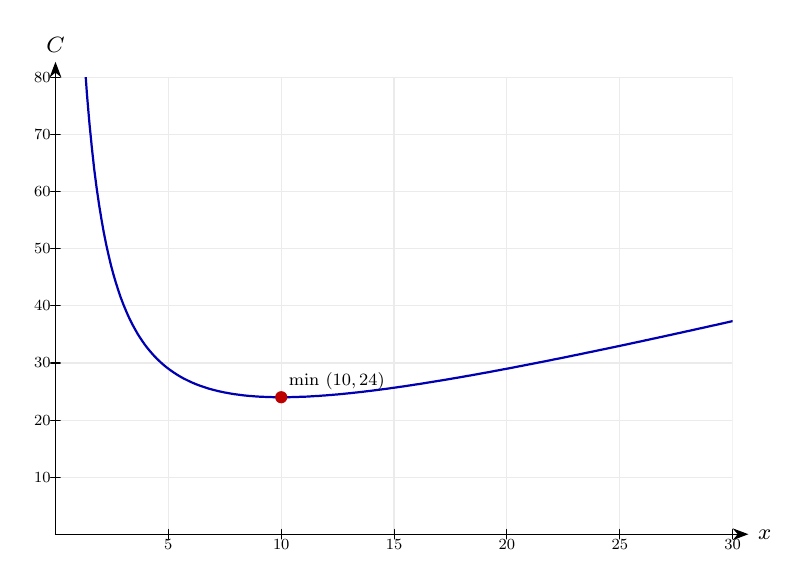
\begin{tikzpicture}[>={Stealth[length=2mm]},font=\footnotesize,line cap=round,line join=round]
\begin{scope}
\clip (0,0) rectangle (8.6,5.8);
\draw[gray!16] (0,0) grid[xstep=1.433,ystep=0.725] (8.6,5.8);
\draw[blue!70!black,thick] (0.031,11.6) -- (0.061,11.6) -- (0.092,11.6) -- (0.123,11.6) -- (0.154,11.6) -- (0.184,11.6) -- (0.215,10.011) -- (0.246,8.81) -- (0.276,7.878) -- (0.307,7.134) -- (0.338,6.527) -- (0.369,6.022) -- (0.399,5.596) -- (0.43,5.232) -- (0.461,4.918) -- (0.491,4.643) -- (0.522,4.402) -- (0.553,4.189) -- (0.584,3.999) -- (0.614,3.829) -- (0.645,3.675) -- (0.676,3.537) -- (0.706,3.411) -- (0.737,3.296) -- (0.768,3.191) -- (0.799,3.095) -- (0.829,3.006) -- (0.86,2.924) -- (0.891,2.849) -- (0.921,2.779) -- (0.952,2.714) -- (0.983,2.653) -- (1.014,2.597) -- (1.044,2.544) -- (1.075,2.495) -- (1.106,2.449) -- (1.136,2.406) -- (1.167,2.366) -- (1.198,2.328) -- (1.229,2.292) -- (1.259,2.259) -- (1.29,2.227) -- (1.321,2.198) -- (1.351,2.17) -- (1.382,2.143) -- (1.413,2.118) -- (1.444,2.095) -- (1.474,2.073) -- (1.505,2.052) -- (1.536,2.032) -- (1.566,2.013) -- (1.597,1.995) -- (1.628,1.978) -- (1.659,1.963) -- (1.689,1.948) -- (1.72,1.933) -- (1.751,1.92) -- (1.781,1.907) -- (1.812,1.895) -- (1.843,1.884) -- (1.874,1.873) -- (1.904,1.863) -- (1.935,1.853) -- (1.966,1.844) -- (1.996,1.836) -- (2.027,1.828) -- (2.058,1.82) -- (2.089,1.813) -- (2.119,1.807) -- (2.15,1.8) -- (2.181,1.795) -- (2.211,1.789) -- (2.242,1.784) -- (2.273,1.779) -- (2.304,1.775) -- (2.334,1.771) -- (2.365,1.767) -- (2.396,1.763) -- (2.426,1.76) -- (2.457,1.757) -- (2.488,1.755) -- (2.519,1.752) -- (2.549,1.75) -- (2.58,1.748) -- (2.611,1.746) -- (2.641,1.745) -- (2.672,1.744) -- (2.703,1.743) -- (2.734,1.742) -- (2.764,1.741) -- (2.795,1.74) -- (2.826,1.74) -- (2.856,1.74) -- (2.887,1.74) -- (2.918,1.74) -- (2.949,1.741) -- (2.979,1.741) -- (3.01,1.742) -- (3.041,1.743) -- (3.071,1.743) -- (3.102,1.745) -- (3.133,1.746) -- (3.164,1.747) -- (3.194,1.748) -- (3.225,1.75) -- (3.256,1.752) -- (3.286,1.754) -- (3.317,1.755) -- (3.348,1.757) -- (3.379,1.76) -- (3.409,1.762) -- (3.44,1.764) -- (3.471,1.767) -- (3.501,1.769) -- (3.532,1.772) -- (3.563,1.774) -- (3.594,1.777) -- (3.624,1.78) -- (3.655,1.783) -- (3.686,1.786) -- (3.716,1.789) -- (3.747,1.792) -- (3.778,1.796) -- (3.809,1.799) -- (3.839,1.802) -- (3.87,1.806) -- (3.901,1.809) -- (3.931,1.813) -- (3.962,1.817) -- (3.993,1.82) -- (4.024,1.824) -- (4.054,1.828) -- (4.085,1.832) -- (4.116,1.836) -- (4.146,1.84) -- (4.177,1.844) -- (4.208,1.848) -- (4.239,1.852) -- (4.269,1.857) -- (4.3,1.861) -- (4.331,1.865) -- (4.361,1.87) -- (4.392,1.874) -- (4.423,1.878) -- (4.454,1.883) -- (4.484,1.888) -- (4.515,1.892) -- (4.546,1.897) -- (4.576,1.902) -- (4.607,1.906) -- (4.638,1.911) -- (4.669,1.916) -- (4.699,1.921) -- (4.73,1.926) -- (4.761,1.931) -- (4.791,1.936) -- (4.822,1.941) -- (4.853,1.946) -- (4.884,1.951) -- (4.914,1.956) -- (4.945,1.961) -- (4.976,1.966) -- (5.006,1.971) -- (5.037,1.977) -- (5.068,1.982) -- (5.099,1.987) -- (5.129,1.992) -- (5.16,1.998) -- (5.191,2.003) -- (5.221,2.009) -- (5.252,2.014) -- (5.283,2.019) -- (5.314,2.025) -- (5.344,2.03) -- (5.375,2.036) -- (5.406,2.042) -- (5.436,2.047) -- (5.467,2.053) -- (5.498,2.058) -- (5.529,2.064) -- (5.559,2.07) -- (5.59,2.076) -- (5.621,2.081) -- (5.651,2.087) -- (5.682,2.093) -- (5.713,2.099) -- (5.744,2.104) -- (5.774,2.11) -- (5.805,2.116) -- (5.836,2.122) -- (5.866,2.128) -- (5.897,2.134) -- (5.928,2.14) -- (5.959,2.146) -- (5.989,2.152) -- (6.02,2.158) -- (6.051,2.164) -- (6.081,2.17) -- (6.112,2.176) -- (6.143,2.182) -- (6.174,2.188) -- (6.204,2.194) -- (6.235,2.2) -- (6.266,2.206) -- (6.296,2.212) -- (6.327,2.219) -- (6.358,2.225) -- (6.389,2.231) -- (6.419,2.237) -- (6.45,2.243) -- (6.481,2.25) -- (6.511,2.256) -- (6.542,2.262) -- (6.573,2.269) -- (6.604,2.275) -- (6.634,2.281) -- (6.665,2.287) -- (6.696,2.294) -- (6.726,2.3) -- (6.757,2.307) -- (6.788,2.313) -- (6.819,2.319) -- (6.849,2.326) -- (6.88,2.332) -- (6.911,2.339) -- (6.941,2.345) -- (6.972,2.351) -- (7.003,2.358) -- (7.034,2.364) -- (7.064,2.371) -- (7.095,2.377) -- (7.126,2.384) -- (7.156,2.39) -- (7.187,2.397) -- (7.218,2.403) -- (7.249,2.41) -- (7.279,2.416) -- (7.31,2.423) -- (7.341,2.43) -- (7.371,2.436) -- (7.402,2.443) -- (7.433,2.449) -- (7.464,2.456) -- (7.494,2.463) -- (7.525,2.469) -- (7.556,2.476) -- (7.586,2.483) -- (7.617,2.489) -- (7.648,2.496) -- (7.679,2.503) -- (7.709,2.509) -- (7.74,2.516) -- (7.771,2.523) -- (7.801,2.529) -- (7.832,2.536) -- (7.863,2.543) -- (7.894,2.55) -- (7.924,2.556) -- (7.955,2.563) -- (7.986,2.57) -- (8.016,2.577) -- (8.047,2.583) -- (8.078,2.59) -- (8.109,2.597) -- (8.139,2.604) -- (8.17,2.611) -- (8.201,2.617) -- (8.231,2.624) -- (8.262,2.631) -- (8.293,2.638) -- (8.324,2.645) -- (8.354,2.652) -- (8.385,2.658) -- (8.416,2.665) -- (8.446,2.672) -- (8.477,2.679) -- (8.508,2.686) -- (8.539,2.693) -- (8.569,2.7) -- (8.6,2.707);
\end{scope}
\draw[->] (0,0) -- (8.8,0) node[right]{$x$};
\draw[->] (0,0) -- (0,6) node[above]{$C$};
\draw (1.433,-0.06) -- (1.433,0.06) node[below=1pt,scale=0.7]{$5$};
\draw (2.867,-0.06) -- (2.867,0.06) node[below=1pt,scale=0.7]{$10$};
\draw (4.3,-0.06) -- (4.3,0.06) node[below=1pt,scale=0.7]{$15$};
\draw (5.733,-0.06) -- (5.733,0.06) node[below=1pt,scale=0.7]{$20$};
\draw (7.167,-0.06) -- (7.167,0.06) node[below=1pt,scale=0.7]{$25$};
\draw (8.6,-0.06) -- (8.6,0.06) node[below=1pt,scale=0.7]{$30$};
\draw (-0.06,0.725) -- (0.06,0.725) node[left=1pt,scale=0.7]{$10$};
\draw (-0.06,1.45) -- (0.06,1.45) node[left=1pt,scale=0.7]{$20$};
\draw (-0.06,2.175) -- (0.06,2.175) node[left=1pt,scale=0.7]{$30$};
\draw (-0.06,2.9) -- (0.06,2.9) node[left=1pt,scale=0.7]{$40$};
\draw (-0.06,3.625) -- (0.06,3.625) node[left=1pt,scale=0.7]{$50$};
\draw (-0.06,4.35) -- (0.06,4.35) node[left=1pt,scale=0.7]{$60$};
\draw (-0.06,5.075) -- (0.06,5.075) node[left=1pt,scale=0.7]{$70$};
\draw (-0.06,5.8) -- (0.06,5.8) node[left=1pt,scale=0.7]{$80$};
\fill[red!75!black] (2.867,1.74) circle (2.2pt);
\node[above right,scale=0.78] at (2.867,1.74) {min $(10,24)$};
\end{tikzpicture}
}
\end{center}
\small The model plotted against its variable, with the key point(s) marked.\normalsize

\medskip\hrule

\section*{Real-Life Problems 44\quad\small\texttt{(d5-044)}}
\addcontentsline{toc}{section}{Real-Life Problems 44 (d5-044)}
\textit{Difficulty: Foundation \quad\textbar\quad Marks: 3}

\question{The cost of producing \( x \) items is \( C(x) = 0.03x^3 - x^2 + 50x + 100 \) pounds. The marginal cost is \( C'(x) \). Find the marginal cost when \( x = 10 \).}

\textbf{Worked solution.}

\textit{Step 1: Differentiate.}
\[\begin{gathered}
C'(x) = 0.09x^2 - 2x + 50
\end{gathered}\]
The marginal cost \( C'(x) \) is the derivative of the total cost --- it approximates the cost of producing one more item beyond the \( x \)th.

\textit{Step 2: Substitute \( x = 10 \).}
\[\begin{gathered}
C'(10) = 9 - 20 + 50 = 39
\end{gathered}\]
At a production level of 10 items, producing one more item costs about \pounds 39.

\begin{answerbox}
\textbf{Final answer:}\quad Marginal cost \(\displaystyle  = \pounds 39 \) per item
\end{answerbox}
\textbf{Diagram.}

\begin{center}
\resizebox{\ifdim\width>\linewidth \linewidth\else \width\fi}{!}{%
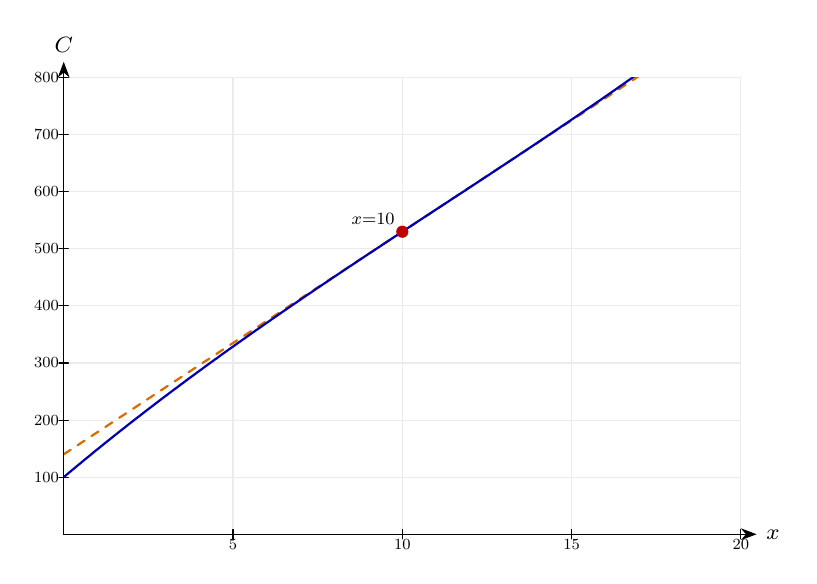
\begin{tikzpicture}[>={Stealth[length=2mm]},font=\footnotesize,line cap=round,line join=round]
\begin{scope}
\clip (0,0) rectangle (8.6,5.8);
\draw[gray!16] (0,0) grid[xstep=2.15,ystep=0.725] (8.6,5.8);
\draw[orange!85!black,thick,dashed] (0,1.015) -- (8.6,6.67);
\draw[blue!70!black,thick] (0,0.725) -- (0.031,0.751) -- (0.061,0.777) -- (0.092,0.802) -- (0.123,0.828) -- (0.154,0.854) -- (0.184,0.879) -- (0.215,0.904) -- (0.246,0.93) -- (0.276,0.955) -- (0.307,0.98) -- (0.338,1.005) -- (0.369,1.031) -- (0.399,1.056) -- (0.43,1.08) -- (0.461,1.105) -- (0.491,1.13) -- (0.522,1.155) -- (0.553,1.18) -- (0.584,1.204) -- (0.614,1.229) -- (0.645,1.253) -- (0.676,1.278) -- (0.706,1.302) -- (0.737,1.326) -- (0.768,1.35) -- (0.799,1.375) -- (0.829,1.399) -- (0.86,1.423) -- (0.891,1.447) -- (0.921,1.471) -- (0.952,1.494) -- (0.983,1.518) -- (1.014,1.542) -- (1.044,1.566) -- (1.075,1.589) -- (1.106,1.613) -- (1.136,1.636) -- (1.167,1.66) -- (1.198,1.683) -- (1.229,1.707) -- (1.259,1.73) -- (1.29,1.753) -- (1.321,1.776) -- (1.351,1.799) -- (1.382,1.822) -- (1.413,1.846) -- (1.444,1.868) -- (1.474,1.891) -- (1.505,1.914) -- (1.536,1.937) -- (1.566,1.96) -- (1.597,1.983) -- (1.628,2.005) -- (1.659,2.028) -- (1.689,2.05) -- (1.72,2.073) -- (1.751,2.095) -- (1.781,2.118) -- (1.812,2.14) -- (1.843,2.163) -- (1.874,2.185) -- (1.904,2.207) -- (1.935,2.229) -- (1.966,2.251) -- (1.996,2.274) -- (2.027,2.296) -- (2.058,2.318) -- (2.089,2.34) -- (2.119,2.362) -- (2.15,2.383) -- (2.181,2.405) -- (2.211,2.427) -- (2.242,2.449) -- (2.273,2.471) -- (2.304,2.492) -- (2.334,2.514) -- (2.365,2.536) -- (2.396,2.557) -- (2.426,2.579) -- (2.457,2.6) -- (2.488,2.622) -- (2.519,2.643) -- (2.549,2.665) -- (2.58,2.686) -- (2.611,2.707) -- (2.641,2.729) -- (2.672,2.75) -- (2.703,2.771) -- (2.734,2.792) -- (2.764,2.814) -- (2.795,2.835) -- (2.826,2.856) -- (2.856,2.877) -- (2.887,2.898) -- (2.918,2.919) -- (2.949,2.94) -- (2.979,2.961) -- (3.01,2.982) -- (3.041,3.003) -- (3.071,3.024) -- (3.102,3.045) -- (3.133,3.065) -- (3.164,3.086) -- (3.194,3.107) -- (3.225,3.128) -- (3.256,3.148) -- (3.286,3.169) -- (3.317,3.19) -- (3.348,3.21) -- (3.379,3.231) -- (3.409,3.252) -- (3.44,3.272) -- (3.471,3.293) -- (3.501,3.313) -- (3.532,3.334) -- (3.563,3.355) -- (3.594,3.375) -- (3.624,3.396) -- (3.655,3.416) -- (3.686,3.436) -- (3.716,3.457) -- (3.747,3.477) -- (3.778,3.498) -- (3.809,3.518) -- (3.839,3.538) -- (3.87,3.559) -- (3.901,3.579) -- (3.931,3.599) -- (3.962,3.62) -- (3.993,3.64) -- (4.024,3.66) -- (4.054,3.681) -- (4.085,3.701) -- (4.116,3.721) -- (4.146,3.741) -- (4.177,3.762) -- (4.208,3.782) -- (4.239,3.802) -- (4.269,3.822) -- (4.3,3.842) -- (4.331,3.863) -- (4.361,3.883) -- (4.392,3.903) -- (4.423,3.923) -- (4.454,3.943) -- (4.484,3.964) -- (4.515,3.984) -- (4.546,4.004) -- (4.576,4.024) -- (4.607,4.044) -- (4.638,4.064) -- (4.669,4.084) -- (4.699,4.105) -- (4.73,4.125) -- (4.761,4.145) -- (4.791,4.165) -- (4.822,4.185) -- (4.853,4.205) -- (4.884,4.225) -- (4.914,4.246) -- (4.945,4.266) -- (4.976,4.286) -- (5.006,4.306) -- (5.037,4.326) -- (5.068,4.346) -- (5.099,4.366) -- (5.129,4.387) -- (5.16,4.407) -- (5.191,4.427) -- (5.221,4.447) -- (5.252,4.467) -- (5.283,4.488) -- (5.314,4.508) -- (5.344,4.528) -- (5.375,4.548) -- (5.406,4.568) -- (5.436,4.589) -- (5.467,4.609) -- (5.498,4.629) -- (5.529,4.65) -- (5.559,4.67) -- (5.59,4.69) -- (5.621,4.71) -- (5.651,4.731) -- (5.682,4.751) -- (5.713,4.771) -- (5.744,4.792) -- (5.774,4.812) -- (5.805,4.833) -- (5.836,4.853) -- (5.866,4.873) -- (5.897,4.894) -- (5.928,4.914) -- (5.959,4.935) -- (5.989,4.955) -- (6.02,4.976) -- (6.051,4.996) -- (6.081,5.017) -- (6.112,5.037) -- (6.143,5.058) -- (6.174,5.079) -- (6.204,5.099) -- (6.235,5.12) -- (6.266,5.141) -- (6.296,5.161) -- (6.327,5.182) -- (6.358,5.203) -- (6.389,5.224) -- (6.419,5.244) -- (6.45,5.265) -- (6.481,5.286) -- (6.511,5.307) -- (6.542,5.328) -- (6.573,5.349) -- (6.604,5.37) -- (6.634,5.391) -- (6.665,5.412) -- (6.696,5.433) -- (6.726,5.454) -- (6.757,5.475) -- (6.788,5.496) -- (6.819,5.517) -- (6.849,5.539) -- (6.88,5.56) -- (6.911,5.581) -- (6.941,5.602) -- (6.972,5.624) -- (7.003,5.645) -- (7.034,5.667) -- (7.064,5.688) -- (7.095,5.709) -- (7.126,5.731) -- (7.156,5.753) -- (7.187,5.774) -- (7.218,5.796) -- (7.249,5.817) -- (7.279,5.839) -- (7.31,5.861) -- (7.341,5.883) -- (7.371,5.904) -- (7.402,5.926) -- (7.433,5.948) -- (7.464,5.97) -- (7.494,5.992) -- (7.525,6.014) -- (7.556,6.036) -- (7.586,6.058) -- (7.617,6.08) -- (7.648,6.103) -- (7.679,6.125) -- (7.709,6.147) -- (7.74,6.169) -- (7.771,6.192) -- (7.801,6.214) -- (7.832,6.237) -- (7.863,6.259) -- (7.894,6.282) -- (7.924,6.304) -- (7.955,6.327) -- (7.986,6.35) -- (8.016,6.373) -- (8.047,6.395) -- (8.078,6.418) -- (8.109,6.441) -- (8.139,6.464) -- (8.17,6.487) -- (8.201,6.51) -- (8.231,6.533) -- (8.262,6.556) -- (8.293,6.58) -- (8.324,6.603) -- (8.354,6.626) -- (8.385,6.65) -- (8.416,6.673) -- (8.446,6.697) -- (8.477,6.72) -- (8.508,6.744) -- (8.539,6.767) -- (8.569,6.791) -- (8.6,6.815);
\end{scope}
\draw[->] (0,0) -- (8.8,0) node[right]{$x$};
\draw[->] (0,0) -- (0,6) node[above]{$C$};
\draw (2.15,-0.06) -- (2.15,0.06) node[below=1pt,scale=0.7]{$5$};
\draw (4.3,-0.06) -- (4.3,0.06) node[below=1pt,scale=0.7]{$10$};
\draw (6.45,-0.06) -- (6.45,0.06) node[below=1pt,scale=0.7]{$15$};
\draw (8.6,-0.06) -- (8.6,0.06) node[below=1pt,scale=0.7]{$20$};
\draw (-0.06,0.725) -- (0.06,0.725) node[left=1pt,scale=0.7]{$100$};
\draw (-0.06,1.45) -- (0.06,1.45) node[left=1pt,scale=0.7]{$200$};
\draw (-0.06,2.175) -- (0.06,2.175) node[left=1pt,scale=0.7]{$300$};
\draw (-0.06,2.9) -- (0.06,2.9) node[left=1pt,scale=0.7]{$400$};
\draw (-0.06,3.625) -- (0.06,3.625) node[left=1pt,scale=0.7]{$500$};
\draw (-0.06,4.35) -- (0.06,4.35) node[left=1pt,scale=0.7]{$600$};
\draw (-0.06,5.075) -- (0.06,5.075) node[left=1pt,scale=0.7]{$700$};
\draw (-0.06,5.8) -- (0.06,5.8) node[left=1pt,scale=0.7]{$800$};
\fill[red!75!black] (4.3,3.842) circle (2.2pt);
\node[above left,scale=0.78] at (4.3,3.842) {$x{=}10$};
\end{tikzpicture}
}
\end{center}
\small The model plotted against its variable, with the key point(s) marked and the tangent (dashed) showing the instantaneous rate.\normalsize

\medskip\hrule

\section*{Real-Life Problems 45\quad\small\texttt{(d5-045)}}
\addcontentsline{toc}{section}{Real-Life Problems 45 (d5-045)}
\textit{Difficulty: Foundation \quad\textbar\quad Marks: 3}

\question{Water flows into a tank so that the volume after \( t \) seconds is \( V = 20t - \dfrac{1}{2}t^2 \) litres. Find the rate at which water is flowing in when \( t = 4 \).}

\textbf{Worked solution.}

\textit{Step 1: Differentiate.}
\[\begin{gathered}
\frac{\mathrm{d}V}{\mathrm{d}t} = 20 - t
\end{gathered}\]
\( \dfrac{\mathrm{d}V}{\mathrm{d}t} \) gives the instantaneous flow rate --- how fast the volume is changing per second.

\textit{Step 2: Substitute \( t = 4 \).}
\[\begin{gathered}
\frac{\mathrm{d}V}{\mathrm{d}t} = 20 - 4 = 16 \text{ litres/s}
\end{gathered}\]
A positive rate means water is flowing in. The rate is decreasing with time, suggesting the inflow is slowing.

\begin{answerbox}
\textbf{Final answer:}\quad \(\displaystyle  16 \) litres per second
\end{answerbox}
\textbf{Diagram.}

\begin{center}
\resizebox{\ifdim\width>\linewidth \linewidth\else \width\fi}{!}{%
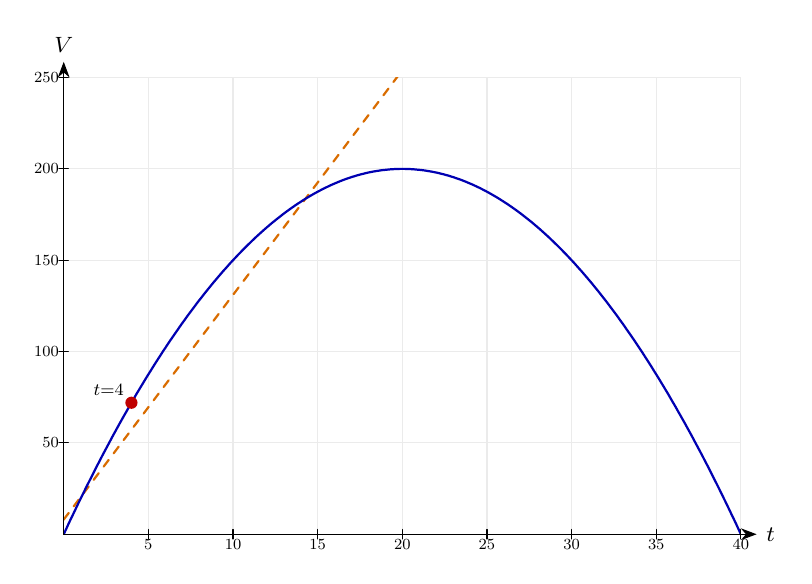
\begin{tikzpicture}[>={Stealth[length=2mm]},font=\footnotesize,line cap=round,line join=round]
\begin{scope}
\clip (0,0) rectangle (8.6,5.8);
\draw[gray!16] (0,0) grid[xstep=1.075,ystep=1.16] (8.6,5.8);
\draw[orange!85!black,thick,dashed] (0,0.186) -- (8.6,11.6);
\draw[blue!70!black,thick] (0,0) -- (0.031,0.066) -- (0.061,0.132) -- (0.092,0.197) -- (0.123,0.261) -- (0.154,0.326) -- (0.184,0.389) -- (0.215,0.452) -- (0.246,0.515) -- (0.276,0.577) -- (0.307,0.639) -- (0.338,0.7) -- (0.369,0.761) -- (0.399,0.822) -- (0.43,0.882) -- (0.461,0.941) -- (0.491,1) -- (0.522,1.058) -- (0.553,1.116) -- (0.584,1.174) -- (0.614,1.231) -- (0.645,1.288) -- (0.676,1.344) -- (0.706,1.399) -- (0.737,1.454) -- (0.768,1.509) -- (0.799,1.563) -- (0.829,1.617) -- (0.86,1.67) -- (0.891,1.723) -- (0.921,1.776) -- (0.952,1.827) -- (0.983,1.879) -- (1.014,1.93) -- (1.044,1.98) -- (1.075,2.03) -- (1.106,2.079) -- (1.136,2.128) -- (1.167,2.177) -- (1.198,2.225) -- (1.229,2.273) -- (1.259,2.32) -- (1.29,2.366) -- (1.321,2.413) -- (1.351,2.458) -- (1.382,2.503) -- (1.413,2.548) -- (1.444,2.592) -- (1.474,2.636) -- (1.505,2.68) -- (1.536,2.722) -- (1.566,2.765) -- (1.597,2.807) -- (1.628,2.848) -- (1.659,2.889) -- (1.689,2.93) -- (1.72,2.97) -- (1.751,3.009) -- (1.781,3.048) -- (1.812,3.087) -- (1.843,3.125) -- (1.874,3.163) -- (1.904,3.2) -- (1.935,3.236) -- (1.966,3.273) -- (1.996,3.308) -- (2.027,3.344) -- (2.058,3.378) -- (2.089,3.413) -- (2.119,3.447) -- (2.15,3.48) -- (2.181,3.513) -- (2.211,3.545) -- (2.242,3.577) -- (2.273,3.609) -- (2.304,3.64) -- (2.334,3.67) -- (2.365,3.7) -- (2.396,3.73) -- (2.426,3.759) -- (2.457,3.788) -- (2.488,3.816) -- (2.519,3.844) -- (2.549,3.871) -- (2.58,3.898) -- (2.611,3.924) -- (2.641,3.95) -- (2.672,3.975) -- (2.703,4) -- (2.734,4.024) -- (2.764,4.048) -- (2.795,4.072) -- (2.826,4.095) -- (2.856,4.117) -- (2.887,4.139) -- (2.918,4.161) -- (2.949,4.182) -- (2.979,4.202) -- (3.01,4.222) -- (3.041,4.242) -- (3.071,4.261) -- (3.102,4.28) -- (3.133,4.298) -- (3.164,4.316) -- (3.194,4.333) -- (3.225,4.35) -- (3.256,4.366) -- (3.286,4.382) -- (3.317,4.398) -- (3.348,4.412) -- (3.379,4.427) -- (3.409,4.441) -- (3.44,4.454) -- (3.471,4.467) -- (3.501,4.48) -- (3.532,4.492) -- (3.563,4.504) -- (3.594,4.515) -- (3.624,4.525) -- (3.655,4.536) -- (3.686,4.545) -- (3.716,4.555) -- (3.747,4.563) -- (3.778,4.572) -- (3.809,4.579) -- (3.839,4.587) -- (3.87,4.594) -- (3.901,4.6) -- (3.931,4.606) -- (3.962,4.611) -- (3.993,4.616) -- (4.024,4.621) -- (4.054,4.625) -- (4.085,4.628) -- (4.116,4.631) -- (4.146,4.634) -- (4.177,4.636) -- (4.208,4.638) -- (4.239,4.639) -- (4.269,4.64) -- (4.3,4.64) -- (4.331,4.64) -- (4.361,4.639) -- (4.392,4.638) -- (4.423,4.636) -- (4.454,4.634) -- (4.484,4.631) -- (4.515,4.628) -- (4.546,4.625) -- (4.576,4.621) -- (4.607,4.616) -- (4.638,4.611) -- (4.669,4.606) -- (4.699,4.6) -- (4.73,4.594) -- (4.761,4.587) -- (4.791,4.579) -- (4.822,4.572) -- (4.853,4.563) -- (4.884,4.555) -- (4.914,4.545) -- (4.945,4.536) -- (4.976,4.525) -- (5.006,4.515) -- (5.037,4.504) -- (5.068,4.492) -- (5.099,4.48) -- (5.129,4.467) -- (5.16,4.454) -- (5.191,4.441) -- (5.221,4.427) -- (5.252,4.412) -- (5.283,4.398) -- (5.314,4.382) -- (5.344,4.366) -- (5.375,4.35) -- (5.406,4.333) -- (5.436,4.316) -- (5.467,4.298) -- (5.498,4.28) -- (5.529,4.261) -- (5.559,4.242) -- (5.59,4.222) -- (5.621,4.202) -- (5.651,4.182) -- (5.682,4.161) -- (5.713,4.139) -- (5.744,4.117) -- (5.774,4.095) -- (5.805,4.072) -- (5.836,4.048) -- (5.866,4.024) -- (5.897,4) -- (5.928,3.975) -- (5.959,3.95) -- (5.989,3.924) -- (6.02,3.898) -- (6.051,3.871) -- (6.081,3.844) -- (6.112,3.816) -- (6.143,3.788) -- (6.174,3.759) -- (6.204,3.73) -- (6.235,3.7) -- (6.266,3.67) -- (6.296,3.64) -- (6.327,3.609) -- (6.358,3.577) -- (6.389,3.545) -- (6.419,3.513) -- (6.45,3.48) -- (6.481,3.447) -- (6.511,3.413) -- (6.542,3.378) -- (6.573,3.344) -- (6.604,3.308) -- (6.634,3.273) -- (6.665,3.236) -- (6.696,3.2) -- (6.726,3.163) -- (6.757,3.125) -- (6.788,3.087) -- (6.819,3.048) -- (6.849,3.009) -- (6.88,2.97) -- (6.911,2.93) -- (6.941,2.889) -- (6.972,2.848) -- (7.003,2.807) -- (7.034,2.765) -- (7.064,2.722) -- (7.095,2.68) -- (7.126,2.636) -- (7.156,2.592) -- (7.187,2.548) -- (7.218,2.503) -- (7.249,2.458) -- (7.279,2.413) -- (7.31,2.366) -- (7.341,2.32) -- (7.371,2.273) -- (7.402,2.225) -- (7.433,2.177) -- (7.464,2.128) -- (7.494,2.079) -- (7.525,2.03) -- (7.556,1.98) -- (7.586,1.93) -- (7.617,1.879) -- (7.648,1.827) -- (7.679,1.776) -- (7.709,1.723) -- (7.74,1.67) -- (7.771,1.617) -- (7.801,1.563) -- (7.832,1.509) -- (7.863,1.454) -- (7.894,1.399) -- (7.924,1.344) -- (7.955,1.288) -- (7.986,1.231) -- (8.016,1.174) -- (8.047,1.116) -- (8.078,1.058) -- (8.109,1) -- (8.139,0.941) -- (8.17,0.882) -- (8.201,0.822) -- (8.231,0.761) -- (8.262,0.7) -- (8.293,0.639) -- (8.324,0.577) -- (8.354,0.515) -- (8.385,0.452) -- (8.416,0.389) -- (8.446,0.326) -- (8.477,0.261) -- (8.508,0.197) -- (8.539,0.132) -- (8.569,0.066) -- (8.6,0);
\end{scope}
\draw[->] (0,0) -- (8.8,0) node[right]{$t$};
\draw[->] (0,0) -- (0,6) node[above]{$V$};
\draw (1.075,-0.06) -- (1.075,0.06) node[below=1pt,scale=0.7]{$5$};
\draw (2.15,-0.06) -- (2.15,0.06) node[below=1pt,scale=0.7]{$10$};
\draw (3.225,-0.06) -- (3.225,0.06) node[below=1pt,scale=0.7]{$15$};
\draw (4.3,-0.06) -- (4.3,0.06) node[below=1pt,scale=0.7]{$20$};
\draw (5.375,-0.06) -- (5.375,0.06) node[below=1pt,scale=0.7]{$25$};
\draw (6.45,-0.06) -- (6.45,0.06) node[below=1pt,scale=0.7]{$30$};
\draw (7.525,-0.06) -- (7.525,0.06) node[below=1pt,scale=0.7]{$35$};
\draw (8.6,-0.06) -- (8.6,0.06) node[below=1pt,scale=0.7]{$40$};
\draw (-0.06,1.16) -- (0.06,1.16) node[left=1pt,scale=0.7]{$50$};
\draw (-0.06,2.32) -- (0.06,2.32) node[left=1pt,scale=0.7]{$100$};
\draw (-0.06,3.48) -- (0.06,3.48) node[left=1pt,scale=0.7]{$150$};
\draw (-0.06,4.64) -- (0.06,4.64) node[left=1pt,scale=0.7]{$200$};
\draw (-0.06,5.8) -- (0.06,5.8) node[left=1pt,scale=0.7]{$250$};
\fill[red!75!black] (0.86,1.67) circle (2.2pt);
\node[above left,scale=0.78] at (0.86,1.67) {$t{=}4$};
\end{tikzpicture}
}
\end{center}
\small The model plotted against its variable, with the key point(s) marked and the tangent (dashed) showing the instantaneous rate.\normalsize

\medskip\hrule

\section*{Real-Life Problems 46\quad\small\texttt{(d5-046)}}
\addcontentsline{toc}{section}{Real-Life Problems 46 (d5-046)}
\textit{Difficulty: Standard \quad\textbar\quad Marks: 5}

\question{A particle moves with displacement \( s = 12t - t^3 \) metres after \( t \) seconds, for \( t \ge 0 \). Find the maximum displacement and the time at which it occurs.}

\textbf{Worked solution.}

\textit{Step 1: Velocity.}
\[\begin{gathered}
v = \frac{\mathrm{d}s}{\mathrm{d}t} = 12 - 3t^2
\end{gathered}\]
At maximum displacement the particle is momentarily stationary, so we will need \( v = 0 \).

\textit{Step 2: Set \( v = 0 \).}
\[\begin{gathered}
12 - 3t^2 = 0 \implies t^2 = 4 \implies t = 2
\end{gathered}\]
Reject \( t = -2 \) since \( t \ge 0 \). At \( t = 2 \) the displacement is neither increasing nor decreasing --- a candidate for maximum.

\textit{Step 3: Maximum displacement.}
\[\begin{gathered}
s = 12(2) - 8 = 16 \text{ m}
\end{gathered}\]
Substitute \( t = 2 \) into the original displacement function.

\textit{Step 4: Confirm maximum.}
\[\begin{gathered}
a = -6t; \, a(2) = -12 < 0 \Rightarrow \text{max} \checkmark
\end{gathered}\]
A negative second derivative \( \left(\dfrac{\mathrm{d}^2 s}{\mathrm{d}t^2}\right) \) at the stationary point confirms it is a maximum, not a minimum.

\begin{answerbox}
\textbf{Final answer:}\quad \(\displaystyle  s_{\max} = 16 \) m at \(\displaystyle  t = 2 \) s
\end{answerbox}
\textbf{Diagram.}

\begin{center}
\resizebox{\ifdim\width>\linewidth \linewidth\else \width\fi}{!}{%
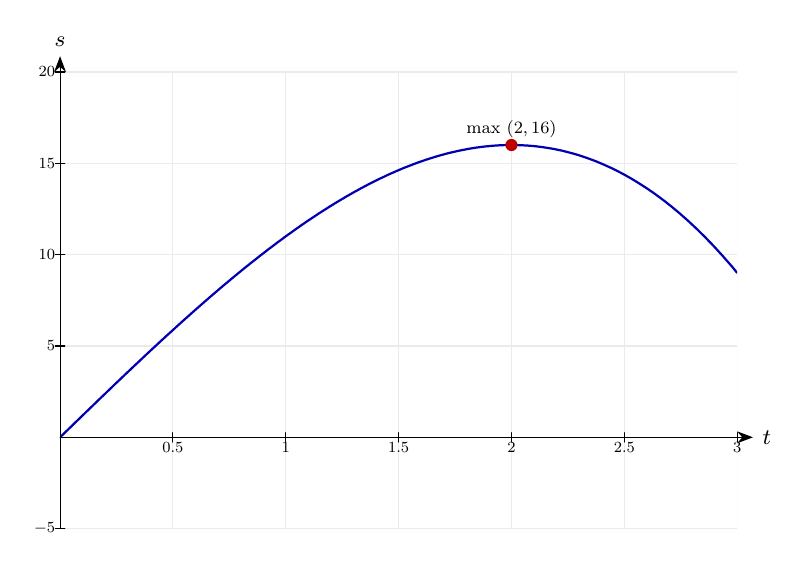
\begin{tikzpicture}[>={Stealth[length=2mm]},font=\footnotesize,line cap=round,line join=round]
\begin{scope}
\clip (0,0) rectangle (8.6,5.8);
\draw[gray!16] (0,0) grid[xstep=1.433,ystep=1.16] (8.6,5.8);
\draw[blue!70!black,thick] (0,1.16) -- (0.031,1.19) -- (0.061,1.22) -- (0.092,1.249) -- (0.123,1.279) -- (0.154,1.309) -- (0.184,1.339) -- (0.215,1.369) -- (0.246,1.398) -- (0.276,1.428) -- (0.307,1.458) -- (0.338,1.488) -- (0.369,1.517) -- (0.399,1.547) -- (0.43,1.577) -- (0.461,1.606) -- (0.491,1.636) -- (0.522,1.666) -- (0.553,1.695) -- (0.584,1.725) -- (0.614,1.754) -- (0.645,1.784) -- (0.676,1.813) -- (0.706,1.843) -- (0.737,1.872) -- (0.768,1.901) -- (0.799,1.931) -- (0.829,1.96) -- (0.86,1.989) -- (0.891,2.018) -- (0.921,2.047) -- (0.952,2.076) -- (0.983,2.105) -- (1.014,2.134) -- (1.044,2.163) -- (1.075,2.192) -- (1.106,2.221) -- (1.136,2.249) -- (1.167,2.278) -- (1.198,2.306) -- (1.229,2.335) -- (1.259,2.363) -- (1.29,2.392) -- (1.321,2.42) -- (1.351,2.448) -- (1.382,2.476) -- (1.413,2.504) -- (1.444,2.532) -- (1.474,2.56) -- (1.505,2.588) -- (1.536,2.616) -- (1.566,2.643) -- (1.597,2.671) -- (1.628,2.698) -- (1.659,2.726) -- (1.689,2.753) -- (1.72,2.78) -- (1.751,2.807) -- (1.781,2.834) -- (1.812,2.861) -- (1.843,2.888) -- (1.874,2.915) -- (1.904,2.941) -- (1.935,2.968) -- (1.966,2.994) -- (1.996,3.02) -- (2.027,3.047) -- (2.058,3.073) -- (2.089,3.099) -- (2.119,3.124) -- (2.15,3.15) -- (2.181,3.176) -- (2.211,3.201) -- (2.242,3.226) -- (2.273,3.252) -- (2.304,3.277) -- (2.334,3.302) -- (2.365,3.327) -- (2.396,3.351) -- (2.426,3.376) -- (2.457,3.4) -- (2.488,3.424) -- (2.519,3.449) -- (2.549,3.473) -- (2.58,3.496) -- (2.611,3.52) -- (2.641,3.544) -- (2.672,3.567) -- (2.703,3.59) -- (2.734,3.614) -- (2.764,3.637) -- (2.795,3.659) -- (2.826,3.682) -- (2.856,3.705) -- (2.887,3.727) -- (2.918,3.749) -- (2.949,3.771) -- (2.979,3.793) -- (3.01,3.815) -- (3.041,3.836) -- (3.071,3.858) -- (3.102,3.879) -- (3.133,3.9) -- (3.164,3.921) -- (3.194,3.941) -- (3.225,3.962) -- (3.256,3.982) -- (3.286,4.002) -- (3.317,4.022) -- (3.348,4.042) -- (3.379,4.061) -- (3.409,4.081) -- (3.44,4.1) -- (3.471,4.119) -- (3.501,4.138) -- (3.532,4.156) -- (3.563,4.175) -- (3.594,4.193) -- (3.624,4.211) -- (3.655,4.229) -- (3.686,4.246) -- (3.716,4.264) -- (3.747,4.281) -- (3.778,4.298) -- (3.809,4.315) -- (3.839,4.331) -- (3.87,4.348) -- (3.901,4.364) -- (3.931,4.38) -- (3.962,4.395) -- (3.993,4.411) -- (4.024,4.426) -- (4.054,4.441) -- (4.085,4.456) -- (4.116,4.47) -- (4.146,4.485) -- (4.177,4.499) -- (4.208,4.513) -- (4.239,4.526) -- (4.269,4.54) -- (4.3,4.553) -- (4.331,4.566) -- (4.361,4.579) -- (4.392,4.591) -- (4.423,4.603) -- (4.454,4.615) -- (4.484,4.627) -- (4.515,4.638) -- (4.546,4.65) -- (4.576,4.661) -- (4.607,4.671) -- (4.638,4.682) -- (4.669,4.692) -- (4.699,4.702) -- (4.73,4.711) -- (4.761,4.721) -- (4.791,4.73) -- (4.822,4.739) -- (4.853,4.747) -- (4.884,4.756) -- (4.914,4.764) -- (4.945,4.772) -- (4.976,4.779) -- (5.006,4.786) -- (5.037,4.793) -- (5.068,4.8) -- (5.099,4.806) -- (5.129,4.812) -- (5.16,4.818) -- (5.191,4.824) -- (5.221,4.829) -- (5.252,4.834) -- (5.283,4.839) -- (5.314,4.843) -- (5.344,4.847) -- (5.375,4.851) -- (5.406,4.854) -- (5.436,4.857) -- (5.467,4.86) -- (5.498,4.863) -- (5.529,4.865) -- (5.559,4.867) -- (5.59,4.869) -- (5.621,4.87) -- (5.651,4.871) -- (5.682,4.872) -- (5.713,4.872) -- (5.744,4.872) -- (5.774,4.872) -- (5.805,4.871) -- (5.836,4.87) -- (5.866,4.869) -- (5.897,4.867) -- (5.928,4.866) -- (5.959,4.863) -- (5.989,4.861) -- (6.02,4.858) -- (6.051,4.855) -- (6.081,4.851) -- (6.112,4.847) -- (6.143,4.843) -- (6.174,4.838) -- (6.204,4.833) -- (6.235,4.828) -- (6.266,4.823) -- (6.296,4.817) -- (6.327,4.81) -- (6.358,4.804) -- (6.389,4.797) -- (6.419,4.789) -- (6.45,4.781) -- (6.481,4.773) -- (6.511,4.765) -- (6.542,4.756) -- (6.573,4.747) -- (6.604,4.737) -- (6.634,4.727) -- (6.665,4.717) -- (6.696,4.706) -- (6.726,4.695) -- (6.757,4.684) -- (6.788,4.672) -- (6.819,4.66) -- (6.849,4.647) -- (6.88,4.634) -- (6.911,4.621) -- (6.941,4.607) -- (6.972,4.593) -- (7.003,4.579) -- (7.034,4.564) -- (7.064,4.549) -- (7.095,4.533) -- (7.126,4.517) -- (7.156,4.501) -- (7.187,4.484) -- (7.218,4.466) -- (7.249,4.449) -- (7.279,4.431) -- (7.31,4.412) -- (7.341,4.393) -- (7.371,4.374) -- (7.402,4.354) -- (7.433,4.334) -- (7.464,4.314) -- (7.494,4.293) -- (7.525,4.272) -- (7.556,4.25) -- (7.586,4.228) -- (7.617,4.205) -- (7.648,4.182) -- (7.679,4.159) -- (7.709,4.135) -- (7.74,4.11) -- (7.771,4.086) -- (7.801,4.06) -- (7.832,4.035) -- (7.863,4.009) -- (7.894,3.982) -- (7.924,3.955) -- (7.955,3.928) -- (7.986,3.9) -- (8.016,3.872) -- (8.047,3.843) -- (8.078,3.814) -- (8.109,3.784) -- (8.139,3.754) -- (8.17,3.724) -- (8.201,3.693) -- (8.231,3.661) -- (8.262,3.63) -- (8.293,3.597) -- (8.324,3.564) -- (8.354,3.531) -- (8.385,3.497) -- (8.416,3.463) -- (8.446,3.428) -- (8.477,3.393) -- (8.508,3.358) -- (8.539,3.322) -- (8.569,3.285) -- (8.6,3.248);
\end{scope}
\draw[->] (0,1.16) -- (8.8,1.16) node[right]{$t$};
\draw[->] (0,0) -- (0,6) node[above]{$s$};
\draw (1.433,1.1) -- (1.433,1.22) node[below=1pt,scale=0.7]{$0.5$};
\draw (2.867,1.1) -- (2.867,1.22) node[below=1pt,scale=0.7]{$1$};
\draw (4.3,1.1) -- (4.3,1.22) node[below=1pt,scale=0.7]{$1.5$};
\draw (5.733,1.1) -- (5.733,1.22) node[below=1pt,scale=0.7]{$2$};
\draw (7.167,1.1) -- (7.167,1.22) node[below=1pt,scale=0.7]{$2.5$};
\draw (8.6,1.1) -- (8.6,1.22) node[below=1pt,scale=0.7]{$3$};
\draw (-0.06,0) -- (0.06,0) node[left=1pt,scale=0.7]{$-5$};
\draw (-0.06,2.32) -- (0.06,2.32) node[left=1pt,scale=0.7]{$5$};
\draw (-0.06,3.48) -- (0.06,3.48) node[left=1pt,scale=0.7]{$10$};
\draw (-0.06,4.64) -- (0.06,4.64) node[left=1pt,scale=0.7]{$15$};
\draw (-0.06,5.8) -- (0.06,5.8) node[left=1pt,scale=0.7]{$20$};
\fill[red!75!black] (5.733,4.872) circle (2.2pt);
\node[above,scale=0.78] at (5.733,4.872) {max $(2,16)$};
\end{tikzpicture}
}
\end{center}
\small The model plotted against its variable, with the key point(s) marked.\normalsize

\medskip\hrule

\section*{Real-Life Problems 47\quad\small\texttt{(d5-047)}}
\addcontentsline{toc}{section}{Real-Life Problems 47 (d5-047)}
\textit{Difficulty: Foundation \quad\textbar\quad Marks: 3}

\question{A firm's revenue from selling \( x \) items is \( R(x) = 200x - 0.5x^2 \) pounds. Find the marginal revenue when \( x = 20 \).}

\textbf{Worked solution.}

\textit{Step 1: Differentiate.}
\[\begin{gathered}
R'(x) = 200 - x
\end{gathered}\]
Marginal revenue is the derivative of total revenue --- it approximates the extra revenue from selling one more item.

\textit{Step 2: Substitute.}
\[\begin{gathered}
R'(20) = 180
\end{gathered}\]
At a sales level of 20 items, the next item adds about \pounds 180 to revenue.

\begin{answerbox}
\textbf{Final answer:}\quad Marginal revenue \(\displaystyle  = \pounds 180 \)
\end{answerbox}
\textbf{Diagram.}

\begin{center}
\resizebox{\ifdim\width>\linewidth \linewidth\else \width\fi}{!}{%
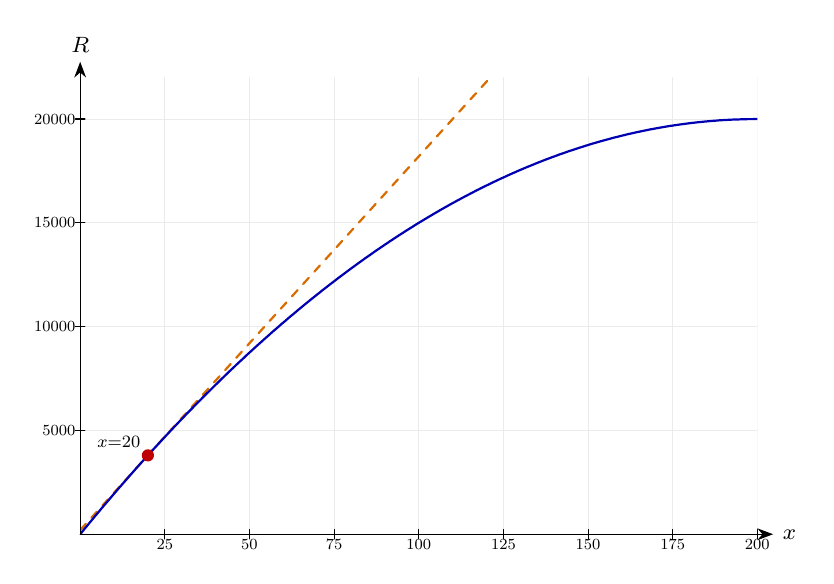
\begin{tikzpicture}[>={Stealth[length=2mm]},font=\footnotesize,line cap=round,line join=round]
\begin{scope}
\clip (0,0) rectangle (8.6,5.8);
\draw[gray!16] (0,0) grid[xstep=1.075,ystep=1.318] (8.6,5.8);
\draw[orange!85!black,thick,dashed] (0,0.053) -- (8.6,9.544);
\draw[blue!70!black,thick] (0,0) -- (0.031,0.038) -- (0.061,0.075) -- (0.092,0.112) -- (0.123,0.15) -- (0.154,0.187) -- (0.184,0.224) -- (0.215,0.26) -- (0.246,0.297) -- (0.276,0.334) -- (0.307,0.37) -- (0.338,0.406) -- (0.369,0.442) -- (0.399,0.478) -- (0.43,0.514) -- (0.461,0.55) -- (0.491,0.585) -- (0.522,0.621) -- (0.553,0.656) -- (0.584,0.691) -- (0.614,0.726) -- (0.645,0.761) -- (0.676,0.796) -- (0.706,0.831) -- (0.737,0.865) -- (0.768,0.9) -- (0.799,0.934) -- (0.829,0.968) -- (0.86,1.002) -- (0.891,1.036) -- (0.921,1.069) -- (0.952,1.103) -- (0.983,1.136) -- (1.014,1.17) -- (1.044,1.203) -- (1.075,1.236) -- (1.106,1.269) -- (1.136,1.301) -- (1.167,1.334) -- (1.198,1.367) -- (1.229,1.399) -- (1.259,1.431) -- (1.29,1.463) -- (1.321,1.495) -- (1.351,1.527) -- (1.382,1.559) -- (1.413,1.59) -- (1.444,1.622) -- (1.474,1.653) -- (1.505,1.684) -- (1.536,1.715) -- (1.566,1.746) -- (1.597,1.777) -- (1.628,1.807) -- (1.659,1.838) -- (1.689,1.868) -- (1.72,1.898) -- (1.751,1.928) -- (1.781,1.958) -- (1.812,1.988) -- (1.843,2.018) -- (1.874,2.047) -- (1.904,2.077) -- (1.935,2.106) -- (1.966,2.135) -- (1.996,2.164) -- (2.027,2.193) -- (2.058,2.221) -- (2.089,2.25) -- (2.119,2.279) -- (2.15,2.307) -- (2.181,2.335) -- (2.211,2.363) -- (2.242,2.391) -- (2.273,2.419) -- (2.304,2.446) -- (2.334,2.474) -- (2.365,2.501) -- (2.396,2.528) -- (2.426,2.556) -- (2.457,2.583) -- (2.488,2.609) -- (2.519,2.636) -- (2.549,2.663) -- (2.58,2.689) -- (2.611,2.715) -- (2.641,2.742) -- (2.672,2.768) -- (2.703,2.793) -- (2.734,2.819) -- (2.764,2.845) -- (2.795,2.87) -- (2.826,2.896) -- (2.856,2.921) -- (2.887,2.946) -- (2.918,2.971) -- (2.949,2.996) -- (2.979,3.02) -- (3.01,3.045) -- (3.041,3.069) -- (3.071,3.094) -- (3.102,3.118) -- (3.133,3.142) -- (3.164,3.166) -- (3.194,3.189) -- (3.225,3.213) -- (3.256,3.237) -- (3.286,3.26) -- (3.317,3.283) -- (3.348,3.306) -- (3.379,3.329) -- (3.409,3.352) -- (3.44,3.375) -- (3.471,3.397) -- (3.501,3.419) -- (3.532,3.442) -- (3.563,3.464) -- (3.594,3.486) -- (3.624,3.508) -- (3.655,3.529) -- (3.686,3.551) -- (3.716,3.572) -- (3.747,3.594) -- (3.778,3.615) -- (3.809,3.636) -- (3.839,3.657) -- (3.87,3.678) -- (3.901,3.698) -- (3.931,3.719) -- (3.962,3.739) -- (3.993,3.76) -- (4.024,3.78) -- (4.054,3.8) -- (4.085,3.819) -- (4.116,3.839) -- (4.146,3.859) -- (4.177,3.878) -- (4.208,3.897) -- (4.239,3.917) -- (4.269,3.936) -- (4.3,3.955) -- (4.331,3.973) -- (4.361,3.992) -- (4.392,4.01) -- (4.423,4.029) -- (4.454,4.047) -- (4.484,4.065) -- (4.515,4.083) -- (4.546,4.101) -- (4.576,4.119) -- (4.607,4.136) -- (4.638,4.154) -- (4.669,4.171) -- (4.699,4.188) -- (4.73,4.205) -- (4.761,4.222) -- (4.791,4.239) -- (4.822,4.255) -- (4.853,4.272) -- (4.884,4.288) -- (4.914,4.304) -- (4.945,4.32) -- (4.976,4.336) -- (5.006,4.352) -- (5.037,4.368) -- (5.068,4.383) -- (5.099,4.399) -- (5.129,4.414) -- (5.16,4.429) -- (5.191,4.444) -- (5.221,4.459) -- (5.252,4.474) -- (5.283,4.488) -- (5.314,4.503) -- (5.344,4.517) -- (5.375,4.531) -- (5.406,4.545) -- (5.436,4.559) -- (5.467,4.573) -- (5.498,4.587) -- (5.529,4.6) -- (5.559,4.614) -- (5.59,4.627) -- (5.621,4.64) -- (5.651,4.653) -- (5.682,4.666) -- (5.713,4.678) -- (5.744,4.691) -- (5.774,4.703) -- (5.805,4.716) -- (5.836,4.728) -- (5.866,4.74) -- (5.897,4.752) -- (5.928,4.764) -- (5.959,4.775) -- (5.989,4.787) -- (6.02,4.798) -- (6.051,4.809) -- (6.081,4.821) -- (6.112,4.831) -- (6.143,4.842) -- (6.174,4.853) -- (6.204,4.864) -- (6.235,4.874) -- (6.266,4.884) -- (6.296,4.894) -- (6.327,4.904) -- (6.358,4.914) -- (6.389,4.924) -- (6.419,4.934) -- (6.45,4.943) -- (6.481,4.953) -- (6.511,4.962) -- (6.542,4.971) -- (6.573,4.98) -- (6.604,4.989) -- (6.634,4.997) -- (6.665,5.006) -- (6.696,5.014) -- (6.726,5.022) -- (6.757,5.031) -- (6.788,5.039) -- (6.819,5.046) -- (6.849,5.054) -- (6.88,5.062) -- (6.911,5.069) -- (6.941,5.077) -- (6.972,5.084) -- (7.003,5.091) -- (7.034,5.098) -- (7.064,5.105) -- (7.095,5.111) -- (7.126,5.118) -- (7.156,5.124) -- (7.187,5.13) -- (7.218,5.137) -- (7.249,5.143) -- (7.279,5.148) -- (7.31,5.154) -- (7.341,5.16) -- (7.371,5.165) -- (7.402,5.17) -- (7.433,5.176) -- (7.464,5.181) -- (7.494,5.186) -- (7.525,5.19) -- (7.556,5.195) -- (7.586,5.199) -- (7.617,5.204) -- (7.648,5.208) -- (7.679,5.212) -- (7.709,5.216) -- (7.74,5.22) -- (7.771,5.224) -- (7.801,5.227) -- (7.832,5.231) -- (7.863,5.234) -- (7.894,5.237) -- (7.924,5.24) -- (7.955,5.243) -- (7.986,5.246) -- (8.016,5.248) -- (8.047,5.251) -- (8.078,5.253) -- (8.109,5.256) -- (8.139,5.258) -- (8.17,5.26) -- (8.201,5.261) -- (8.231,5.263) -- (8.262,5.265) -- (8.293,5.266) -- (8.324,5.267) -- (8.354,5.268) -- (8.385,5.269) -- (8.416,5.27) -- (8.446,5.271) -- (8.477,5.272) -- (8.508,5.272) -- (8.539,5.272) -- (8.569,5.273) -- (8.6,5.273);
\end{scope}
\draw[->] (0,0) -- (8.8,0) node[right]{$x$};
\draw[->] (0,0) -- (0,6) node[above]{$R$};
\draw (1.075,-0.06) -- (1.075,0.06) node[below=1pt,scale=0.7]{$25$};
\draw (2.15,-0.06) -- (2.15,0.06) node[below=1pt,scale=0.7]{$50$};
\draw (3.225,-0.06) -- (3.225,0.06) node[below=1pt,scale=0.7]{$75$};
\draw (4.3,-0.06) -- (4.3,0.06) node[below=1pt,scale=0.7]{$100$};
\draw (5.375,-0.06) -- (5.375,0.06) node[below=1pt,scale=0.7]{$125$};
\draw (6.45,-0.06) -- (6.45,0.06) node[below=1pt,scale=0.7]{$150$};
\draw (7.525,-0.06) -- (7.525,0.06) node[below=1pt,scale=0.7]{$175$};
\draw (8.6,-0.06) -- (8.6,0.06) node[below=1pt,scale=0.7]{$200$};
\draw (-0.06,1.318) -- (0.06,1.318) node[left=1pt,scale=0.7]{$5000$};
\draw (-0.06,2.636) -- (0.06,2.636) node[left=1pt,scale=0.7]{$10000$};
\draw (-0.06,3.955) -- (0.06,3.955) node[left=1pt,scale=0.7]{$15000$};
\draw (-0.06,5.273) -- (0.06,5.273) node[left=1pt,scale=0.7]{$20000$};
\fill[red!75!black] (0.86,1.002) circle (2.2pt);
\node[above left,scale=0.78] at (0.86,1.002) {$x{=}20$};
\end{tikzpicture}
}
\end{center}
\small The model plotted against its variable, with the key point(s) marked and the tangent (dashed) showing the instantaneous rate.\normalsize

\medskip\hrule

\section*{Real-Life Problems 48\quad\small\texttt{(d5-048)}}
\addcontentsline{toc}{section}{Real-Life Problems 48 (d5-048)}
\textit{Difficulty: Standard \quad\textbar\quad Marks: 5}

\question{A stone is dropped from a cliff. Its height above the ground after \( t \) seconds is \( h = 80 - 5t^2 \) metres. (a) Find the time taken for the stone to reach the ground. (b) Find the speed of the stone when it hits the ground.}

\textbf{Worked solution.}

\textit{Step 1: (a) Set \( h = 0 \).}
\[\begin{gathered}
80 - 5t^2 = 0 \implies t^2 = 16 \implies t = 4 \text{ s}
\end{gathered}\]
The stone hits the ground when its height is zero. Take the positive root since \( t \ge 0 \).

\textit{Step 2: (b) Velocity.}
\[\begin{gathered}
v = \frac{\mathrm{d}h}{\mathrm{d}t} = -10t
\end{gathered}\]
Velocity is the rate of change of height. The negative sign reflects that height is decreasing --- the stone is moving downwards.

\textit{Step 3: Speed at \( t = 4 \).}
\[\begin{gathered}
v = -40 \Rightarrow \text{speed} = 40 \text{ ms}^{-1}
\end{gathered}\]
Speed is the magnitude of velocity (no direction). The minus sign is dropped when reporting speed.

\begin{answerbox}
\textbf{Final answer:}\quad (a) \(\displaystyle  t = 4 \) s \\[3pt]  (b) \(\displaystyle  40 \text{ ms}^{-1} \)
\end{answerbox}
\textbf{Diagram.}

\begin{center}
\resizebox{\ifdim\width>\linewidth \linewidth\else \width\fi}{!}{%
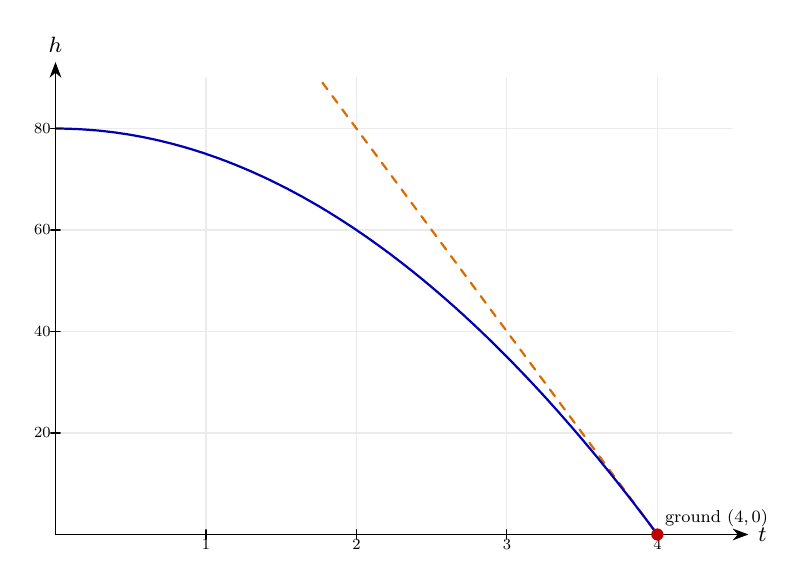
\begin{tikzpicture}[>={Stealth[length=2mm]},font=\footnotesize,line cap=round,line join=round]
\begin{scope}
\clip (0,0) rectangle (8.6,5.8);
\draw[gray!16] (0,0) grid[xstep=1.911,ystep=1.289] (8.6,5.8);
\draw[orange!85!black,thick,dashed] (0,10.311) -- (8.6,-1.289);
\draw[blue!70!black,thick] (0,5.156) -- (0.031,5.155) -- (0.061,5.155) -- (0.092,5.155) -- (0.123,5.154) -- (0.154,5.153) -- (0.184,5.153) -- (0.215,5.151) -- (0.246,5.15) -- (0.276,5.149) -- (0.307,5.147) -- (0.338,5.145) -- (0.369,5.144) -- (0.399,5.141) -- (0.43,5.139) -- (0.461,5.137) -- (0.491,5.134) -- (0.522,5.132) -- (0.553,5.129) -- (0.584,5.126) -- (0.614,5.122) -- (0.645,5.119) -- (0.676,5.115) -- (0.706,5.112) -- (0.737,5.108) -- (0.768,5.104) -- (0.799,5.099) -- (0.829,5.095) -- (0.86,5.09) -- (0.891,5.086) -- (0.921,5.081) -- (0.952,5.076) -- (0.983,5.07) -- (1.014,5.065) -- (1.044,5.059) -- (1.075,5.054) -- (1.106,5.048) -- (1.136,5.042) -- (1.167,5.035) -- (1.198,5.029) -- (1.229,5.022) -- (1.259,5.016) -- (1.29,5.009) -- (1.321,5.002) -- (1.351,4.994) -- (1.382,4.987) -- (1.413,4.979) -- (1.444,4.972) -- (1.474,4.964) -- (1.505,4.956) -- (1.536,4.947) -- (1.566,4.939) -- (1.597,4.931) -- (1.628,4.922) -- (1.659,4.913) -- (1.689,4.904) -- (1.72,4.895) -- (1.751,4.885) -- (1.781,4.876) -- (1.812,4.866) -- (1.843,4.856) -- (1.874,4.846) -- (1.904,4.836) -- (1.935,4.825) -- (1.966,4.815) -- (1.996,4.804) -- (2.027,4.793) -- (2.058,4.782) -- (2.089,4.771) -- (2.119,4.759) -- (2.15,4.748) -- (2.181,4.736) -- (2.211,4.724) -- (2.242,4.712) -- (2.273,4.7) -- (2.304,4.687) -- (2.334,4.675) -- (2.365,4.662) -- (2.396,4.649) -- (2.426,4.636) -- (2.457,4.623) -- (2.488,4.61) -- (2.519,4.596) -- (2.549,4.582) -- (2.58,4.568) -- (2.611,4.554) -- (2.641,4.54) -- (2.672,4.526) -- (2.703,4.511) -- (2.734,4.496) -- (2.764,4.481) -- (2.795,4.466) -- (2.826,4.451) -- (2.856,4.436) -- (2.887,4.42) -- (2.918,4.404) -- (2.949,4.389) -- (2.979,4.372) -- (3.01,4.356) -- (3.041,4.34) -- (3.071,4.323) -- (3.102,4.307) -- (3.133,4.29) -- (3.164,4.273) -- (3.194,4.255) -- (3.225,4.238) -- (3.256,4.22) -- (3.286,4.203) -- (3.317,4.185) -- (3.348,4.167) -- (3.379,4.149) -- (3.409,4.13) -- (3.44,4.112) -- (3.471,4.093) -- (3.501,4.074) -- (3.532,4.055) -- (3.563,4.036) -- (3.594,4.016) -- (3.624,3.997) -- (3.655,3.977) -- (3.686,3.957) -- (3.716,3.937) -- (3.747,3.917) -- (3.778,3.896) -- (3.809,3.876) -- (3.839,3.855) -- (3.87,3.834) -- (3.901,3.813) -- (3.931,3.792) -- (3.962,3.771) -- (3.993,3.749) -- (4.024,3.727) -- (4.054,3.705) -- (4.085,3.683) -- (4.116,3.661) -- (4.146,3.639) -- (4.177,3.616) -- (4.208,3.593) -- (4.239,3.571) -- (4.269,3.548) -- (4.3,3.524) -- (4.331,3.501) -- (4.361,3.477) -- (4.392,3.454) -- (4.423,3.43) -- (4.454,3.406) -- (4.484,3.381) -- (4.515,3.357) -- (4.546,3.333) -- (4.576,3.308) -- (4.607,3.283) -- (4.638,3.258) -- (4.669,3.233) -- (4.699,3.207) -- (4.73,3.182) -- (4.761,3.156) -- (4.791,3.13) -- (4.822,3.104) -- (4.853,3.078) -- (4.884,3.051) -- (4.914,3.025) -- (4.945,2.998) -- (4.976,2.971) -- (5.006,2.944) -- (5.037,2.917) -- (5.068,2.89) -- (5.099,2.862) -- (5.129,2.834) -- (5.16,2.807) -- (5.191,2.779) -- (5.221,2.75) -- (5.252,2.722) -- (5.283,2.693) -- (5.314,2.665) -- (5.344,2.636) -- (5.375,2.607) -- (5.406,2.578) -- (5.436,2.548) -- (5.467,2.519) -- (5.498,2.489) -- (5.529,2.459) -- (5.559,2.429) -- (5.59,2.399) -- (5.621,2.368) -- (5.651,2.338) -- (5.682,2.307) -- (5.713,2.276) -- (5.744,2.245) -- (5.774,2.214) -- (5.805,2.183) -- (5.836,2.151) -- (5.866,2.119) -- (5.897,2.087) -- (5.928,2.055) -- (5.959,2.023) -- (5.989,1.991) -- (6.02,1.958) -- (6.051,1.926) -- (6.081,1.893) -- (6.112,1.86) -- (6.143,1.826) -- (6.174,1.793) -- (6.204,1.76) -- (6.235,1.726) -- (6.266,1.692) -- (6.296,1.658) -- (6.327,1.624) -- (6.358,1.589) -- (6.389,1.555) -- (6.419,1.52) -- (6.45,1.485) -- (6.481,1.45) -- (6.511,1.415) -- (6.542,1.38) -- (6.573,1.344) -- (6.604,1.308) -- (6.634,1.273) -- (6.665,1.236) -- (6.696,1.2) -- (6.726,1.164) -- (6.757,1.127) -- (6.788,1.091) -- (6.819,1.054) -- (6.849,1.017) -- (6.88,0.98) -- (6.911,0.942) -- (6.941,0.905) -- (6.972,0.867) -- (7.003,0.829) -- (7.034,0.791) -- (7.064,0.753) -- (7.095,0.714) -- (7.126,0.676) -- (7.156,0.637) -- (7.187,0.598) -- (7.218,0.559) -- (7.249,0.52) -- (7.279,0.481) -- (7.31,0.441) -- (7.341,0.402) -- (7.371,0.362) -- (7.402,0.322) -- (7.433,0.281) -- (7.464,0.241) -- (7.494,0.201) -- (7.525,0.16) -- (7.556,0.119) -- (7.586,0.078) -- (7.617,0.037) -- (7.648,-0.005) -- (7.679,-0.046) -- (7.709,-0.088) -- (7.74,-0.13) -- (7.771,-0.172) -- (7.801,-0.214) -- (7.832,-0.256) -- (7.863,-0.299) -- (7.894,-0.342) -- (7.924,-0.384) -- (7.955,-0.427) -- (7.986,-0.471) -- (8.016,-0.514) -- (8.047,-0.557) -- (8.078,-0.601) -- (8.109,-0.645) -- (8.139,-0.689) -- (8.17,-0.733) -- (8.201,-0.778) -- (8.231,-0.822) -- (8.262,-0.867) -- (8.293,-0.912) -- (8.324,-0.957) -- (8.354,-1.002) -- (8.385,-1.047) -- (8.416,-1.093) -- (8.446,-1.138) -- (8.477,-1.184) -- (8.508,-1.23) -- (8.539,-1.277) -- (8.569,-1.323) -- (8.6,-1.369);
\end{scope}
\draw[->] (0,0) -- (8.8,0) node[right]{$t$};
\draw[->] (0,0) -- (0,6) node[above]{$h$};
\draw (1.911,-0.06) -- (1.911,0.06) node[below=1pt,scale=0.7]{$1$};
\draw (3.822,-0.06) -- (3.822,0.06) node[below=1pt,scale=0.7]{$2$};
\draw (5.733,-0.06) -- (5.733,0.06) node[below=1pt,scale=0.7]{$3$};
\draw (7.644,-0.06) -- (7.644,0.06) node[below=1pt,scale=0.7]{$4$};
\draw (-0.06,1.289) -- (0.06,1.289) node[left=1pt,scale=0.7]{$20$};
\draw (-0.06,2.578) -- (0.06,2.578) node[left=1pt,scale=0.7]{$40$};
\draw (-0.06,3.867) -- (0.06,3.867) node[left=1pt,scale=0.7]{$60$};
\draw (-0.06,5.156) -- (0.06,5.156) node[left=1pt,scale=0.7]{$80$};
\fill[red!75!black] (7.644,0) circle (2.2pt);
\node[above right,scale=0.78] at (7.644,0) {ground $(4,0)$};
\end{tikzpicture}
}
\end{center}
\small The model plotted against its variable, with the key point(s) marked and the tangent (dashed) showing the instantaneous rate.\normalsize

\medskip\hrule

\section*{Real-Life Problems 49\quad\small\texttt{(d5-049)}}
\addcontentsline{toc}{section}{Real-Life Problems 49 (d5-049)}
\textit{Difficulty: Standard \quad\textbar\quad Marks: 7}

\question{An open cylindrical container (no lid) has volume \( 27\pi \) cm\(^3\). The radius is \( r \) cm and the height is \( h \) cm. Find the radius and height that minimise the surface area.}

\textbf{Worked solution.}

\textit{Step 1: Volume.}
\[\begin{gathered}
\pi r^2 h = 27\pi \implies h = \frac{27}{r^2}
\end{gathered}\]
Use the fixed-volume constraint to eliminate \( h \), so the surface area becomes a single-variable function.

\textit{Step 2: Surface area (base + curved).}
\[\begin{gathered}
A = \pi r^2 + 2\pi r h = \pi r^2 + \frac{54\pi}{r}
\end{gathered}\]
There is no top (open container), so we have only one circular face plus the curved side. Substitute \( h = 27/r^2 \).

\textit{Step 3: Differentiate.}
\[\begin{gathered}
\frac{\mathrm{d}A}{\mathrm{d}r} = 2\pi r - \frac{54\pi}{r^2}
\end{gathered}\]
Power rule: write \( \dfrac{54\pi}{r} = 54\pi r^{-1} \), whose derivative is \( -54\pi r^{-2} \).

\textit{Step 4: Set to zero.}
\[\begin{gathered}
2\pi r = \frac{54\pi}{r^2} \implies r^3 = 27 \implies r = 3
\end{gathered}\]
At the minimising radius the surface area is momentarily neither growing nor shrinking. Multiply by \( r^2 \) and divide by \( 2\pi \) to isolate \( r^3 \).

\textit{Step 5: Find \( h \) and \( A \).}
\[\begin{gathered}
h = 3; \quad A = 9\pi + 18\pi = 27\pi \text{ cm}^2
\end{gathered}\]
For an open cylinder, the optimal shape has \( h = r \) --- height equals radius --- half the height of the closed case.

\begin{answerbox}
\textbf{Final answer:}\quad \(\displaystyle  r = 3 \) cm, \(\displaystyle  h = 3 \) cm, \(\displaystyle  A_{\min} = 27\pi \text{ cm}^2 \)
\end{answerbox}
\textbf{Diagram.}

\begin{center}
\resizebox{\ifdim\width>\linewidth \linewidth\else \width\fi}{!}{%
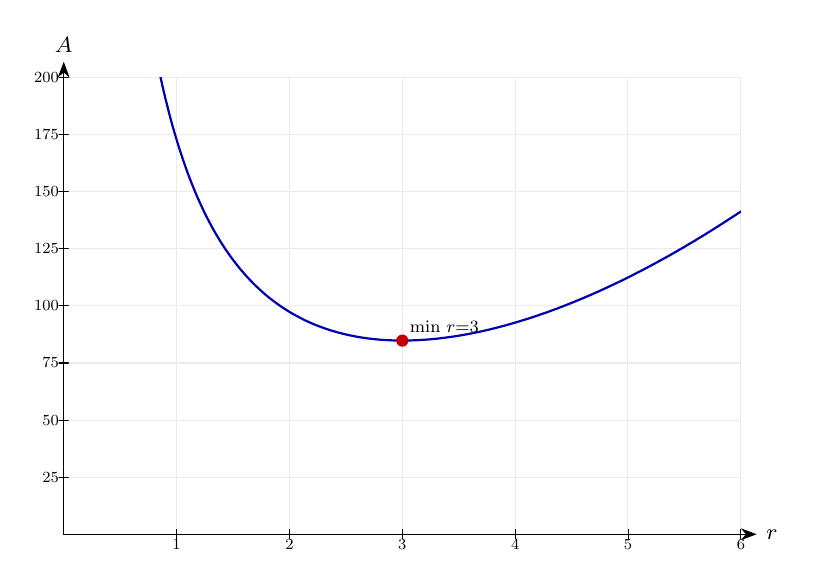
\begin{tikzpicture}[>={Stealth[length=2mm]},font=\footnotesize,line cap=round,line join=round]
\begin{scope}
\clip (0,0) rectangle (8.6,5.8);
\draw[gray!16] (0,0) grid[xstep=1.433,ystep=0.725] (8.6,5.8);
\draw[blue!70!black,thick] (0.031,11.6) -- (0.061,11.6) -- (0.092,11.6) -- (0.123,11.6) -- (0.154,11.6) -- (0.184,11.6) -- (0.215,11.6) -- (0.246,11.6) -- (0.276,11.6) -- (0.307,11.6) -- (0.338,11.6) -- (0.369,11.6) -- (0.399,11.6) -- (0.43,11.6) -- (0.461,11.6) -- (0.491,11.6) -- (0.522,11.6) -- (0.553,11.6) -- (0.584,11.6) -- (0.614,11.496) -- (0.645,10.951) -- (0.676,10.456) -- (0.706,10.004) -- (0.737,9.59) -- (0.768,9.21) -- (0.799,8.859) -- (0.829,8.534) -- (0.86,8.232) -- (0.891,7.952) -- (0.921,7.691) -- (0.952,7.446) -- (0.983,7.217) -- (1.014,7.003) -- (1.044,6.801) -- (1.075,6.611) -- (1.106,6.432) -- (1.136,6.262) -- (1.167,6.102) -- (1.198,5.95) -- (1.229,5.807) -- (1.259,5.67) -- (1.29,5.54) -- (1.321,5.417) -- (1.351,5.299) -- (1.382,5.187) -- (1.413,5.08) -- (1.444,4.977) -- (1.474,4.879) -- (1.505,4.786) -- (1.536,4.696) -- (1.566,4.611) -- (1.597,4.528) -- (1.628,4.449) -- (1.659,4.374) -- (1.689,4.301) -- (1.72,4.231) -- (1.751,4.164) -- (1.781,4.099) -- (1.812,4.037) -- (1.843,3.977) -- (1.874,3.919) -- (1.904,3.864) -- (1.935,3.81) -- (1.966,3.759) -- (1.996,3.709) -- (2.027,3.661) -- (2.058,3.614) -- (2.089,3.57) -- (2.119,3.527) -- (2.15,3.485) -- (2.181,3.445) -- (2.211,3.406) -- (2.242,3.368) -- (2.273,3.332) -- (2.304,3.296) -- (2.334,3.263) -- (2.365,3.23) -- (2.396,3.198) -- (2.426,3.167) -- (2.457,3.138) -- (2.488,3.109) -- (2.519,3.081) -- (2.549,3.054) -- (2.58,3.028) -- (2.611,3.003) -- (2.641,2.979) -- (2.672,2.956) -- (2.703,2.933) -- (2.734,2.911) -- (2.764,2.89) -- (2.795,2.869) -- (2.826,2.85) -- (2.856,2.831) -- (2.887,2.812) -- (2.918,2.794) -- (2.949,2.777) -- (2.979,2.761) -- (3.01,2.745) -- (3.041,2.729) -- (3.071,2.714) -- (3.102,2.7) -- (3.133,2.686) -- (3.164,2.673) -- (3.194,2.66) -- (3.225,2.648) -- (3.256,2.636) -- (3.286,2.625) -- (3.317,2.614) -- (3.348,2.603) -- (3.379,2.593) -- (3.409,2.584) -- (3.44,2.575) -- (3.471,2.566) -- (3.501,2.558) -- (3.532,2.55) -- (3.563,2.542) -- (3.594,2.535) -- (3.624,2.528) -- (3.655,2.522) -- (3.686,2.516) -- (3.716,2.51) -- (3.747,2.505) -- (3.778,2.499) -- (3.809,2.495) -- (3.839,2.49) -- (3.87,2.486) -- (3.901,2.483) -- (3.931,2.479) -- (3.962,2.476) -- (3.993,2.473) -- (4.024,2.47) -- (4.054,2.468) -- (4.085,2.466) -- (4.116,2.465) -- (4.146,2.463) -- (4.177,2.462) -- (4.208,2.461) -- (4.239,2.46) -- (4.269,2.46) -- (4.3,2.46) -- (4.331,2.46) -- (4.361,2.46) -- (4.392,2.461) -- (4.423,2.462) -- (4.454,2.463) -- (4.484,2.464) -- (4.515,2.466) -- (4.546,2.468) -- (4.576,2.47) -- (4.607,2.472) -- (4.638,2.474) -- (4.669,2.477) -- (4.699,2.48) -- (4.73,2.483) -- (4.761,2.486) -- (4.791,2.49) -- (4.822,2.494) -- (4.853,2.497) -- (4.884,2.502) -- (4.914,2.506) -- (4.945,2.51) -- (4.976,2.515) -- (5.006,2.52) -- (5.037,2.525) -- (5.068,2.53) -- (5.099,2.536) -- (5.129,2.541) -- (5.16,2.547) -- (5.191,2.553) -- (5.221,2.56) -- (5.252,2.566) -- (5.283,2.572) -- (5.314,2.579) -- (5.344,2.586) -- (5.375,2.593) -- (5.406,2.6) -- (5.436,2.608) -- (5.467,2.615) -- (5.498,2.623) -- (5.529,2.631) -- (5.559,2.639) -- (5.59,2.647) -- (5.621,2.656) -- (5.651,2.664) -- (5.682,2.673) -- (5.713,2.682) -- (5.744,2.691) -- (5.774,2.7) -- (5.805,2.709) -- (5.836,2.719) -- (5.866,2.728) -- (5.897,2.738) -- (5.928,2.748) -- (5.959,2.758) -- (5.989,2.768) -- (6.02,2.778) -- (6.051,2.789) -- (6.081,2.8) -- (6.112,2.81) -- (6.143,2.821) -- (6.174,2.832) -- (6.204,2.844) -- (6.235,2.855) -- (6.266,2.866) -- (6.296,2.878) -- (6.327,2.89) -- (6.358,2.902) -- (6.389,2.914) -- (6.419,2.926) -- (6.45,2.938) -- (6.481,2.951) -- (6.511,2.963) -- (6.542,2.976) -- (6.573,2.989) -- (6.604,3.002) -- (6.634,3.015) -- (6.665,3.028) -- (6.696,3.041) -- (6.726,3.055) -- (6.757,3.068) -- (6.788,3.082) -- (6.819,3.096) -- (6.849,3.11) -- (6.88,3.124) -- (6.911,3.138) -- (6.941,3.153) -- (6.972,3.167) -- (7.003,3.182) -- (7.034,3.196) -- (7.064,3.211) -- (7.095,3.226) -- (7.126,3.241) -- (7.156,3.257) -- (7.187,3.272) -- (7.218,3.287) -- (7.249,3.303) -- (7.279,3.319) -- (7.31,3.334) -- (7.341,3.35) -- (7.371,3.366) -- (7.402,3.382) -- (7.433,3.399) -- (7.464,3.415) -- (7.494,3.432) -- (7.525,3.448) -- (7.556,3.465) -- (7.586,3.482) -- (7.617,3.499) -- (7.648,3.516) -- (7.679,3.533) -- (7.709,3.55) -- (7.74,3.568) -- (7.771,3.585) -- (7.801,3.603) -- (7.832,3.621) -- (7.863,3.638) -- (7.894,3.656) -- (7.924,3.675) -- (7.955,3.693) -- (7.986,3.711) -- (8.016,3.729) -- (8.047,3.748) -- (8.078,3.767) -- (8.109,3.785) -- (8.139,3.804) -- (8.17,3.823) -- (8.201,3.842) -- (8.231,3.861) -- (8.262,3.881) -- (8.293,3.9) -- (8.324,3.92) -- (8.354,3.939) -- (8.385,3.959) -- (8.416,3.979) -- (8.446,3.999) -- (8.477,4.019) -- (8.508,4.039) -- (8.539,4.059) -- (8.569,4.079) -- (8.6,4.1);
\end{scope}
\draw[->] (0,0) -- (8.8,0) node[right]{$r$};
\draw[->] (0,0) -- (0,6) node[above]{$A$};
\draw (1.433,-0.06) -- (1.433,0.06) node[below=1pt,scale=0.7]{$1$};
\draw (2.867,-0.06) -- (2.867,0.06) node[below=1pt,scale=0.7]{$2$};
\draw (4.3,-0.06) -- (4.3,0.06) node[below=1pt,scale=0.7]{$3$};
\draw (5.733,-0.06) -- (5.733,0.06) node[below=1pt,scale=0.7]{$4$};
\draw (7.167,-0.06) -- (7.167,0.06) node[below=1pt,scale=0.7]{$5$};
\draw (8.6,-0.06) -- (8.6,0.06) node[below=1pt,scale=0.7]{$6$};
\draw (-0.06,0.725) -- (0.06,0.725) node[left=1pt,scale=0.7]{$25$};
\draw (-0.06,1.45) -- (0.06,1.45) node[left=1pt,scale=0.7]{$50$};
\draw (-0.06,2.175) -- (0.06,2.175) node[left=1pt,scale=0.7]{$75$};
\draw (-0.06,2.9) -- (0.06,2.9) node[left=1pt,scale=0.7]{$100$};
\draw (-0.06,3.625) -- (0.06,3.625) node[left=1pt,scale=0.7]{$125$};
\draw (-0.06,4.35) -- (0.06,4.35) node[left=1pt,scale=0.7]{$150$};
\draw (-0.06,5.075) -- (0.06,5.075) node[left=1pt,scale=0.7]{$175$};
\draw (-0.06,5.8) -- (0.06,5.8) node[left=1pt,scale=0.7]{$200$};
\fill[red!75!black] (4.3,2.459) circle (2.2pt);
\node[above right,scale=0.78] at (4.3,2.459) {min $r{=}3$};
\end{tikzpicture}
}
\end{center}
\small The model plotted against its variable, with the key point(s) marked.\normalsize

\medskip\hrule

\section*{Real-Life Problems 50\quad\small\texttt{(d5-050)}}
\addcontentsline{toc}{section}{Real-Life Problems 50 (d5-050)}
\textit{Difficulty: Standard \quad\textbar\quad Marks: 6}

\question{A farmer has 60 m of fencing and wants to enclose a rectangular area against a long straight wall, using the wall as one side. Find the dimensions and the maximum area.}

\textbf{Worked solution.}

\textit{Step 1: Let width be \( w \), length parallel to wall be \( L \).}
\[\begin{gathered}
2w + L = 60 \implies L = 60 - 2w
\end{gathered}\]
Only three sides need fencing --- two widths and one length --- because the wall replaces the fourth side.

\textit{Step 2: Area.}
\[\begin{gathered}
A = wL = w(60 - 2w) = 60w - 2w^2
\end{gathered}\]
Substitute \( L \) into \( A = wL \) to express area in one variable, ready for differentiation.

\textit{Step 3: Differentiate.}
\[\begin{gathered}
\frac{\mathrm{d}A}{\mathrm{d}w} = 60 - 4w = 0 \implies w = 15
\end{gathered}\]
A stationary point of the area. Notice the length comes out twice the width --- the classic result for a three-sided enclosure.

\textit{Step 4: Find \( L \) and \( A \).}
\[\begin{gathered}
L = 30; \quad A = 15 \cdot 30 = 450 \text{ m}^2
\end{gathered}\]
Substitute \( w = 15 \) into \( L = 60 - 2w \) and then into \( A = wL \).

\textit{Step 5: Confirm maximum.}
\[\begin{gathered}
\frac{\mathrm{d}^2A}{\mathrm{d}w^2} = -4 < 0 \Rightarrow \text{max} \checkmark
\end{gathered}\]
Negative second derivative confirms the stationary point is a maximum, not a minimum.

\begin{answerbox}
\textbf{Final answer:}\quad \(\displaystyle  w = 15 \) m, \(\displaystyle  L = 30 \) m, \(\displaystyle  A_{\max} = 450 \text{ m}^2 \)
\end{answerbox}
\textbf{Diagram.}

\begin{center}
\resizebox{\ifdim\width>\linewidth \linewidth\else \width\fi}{!}{%
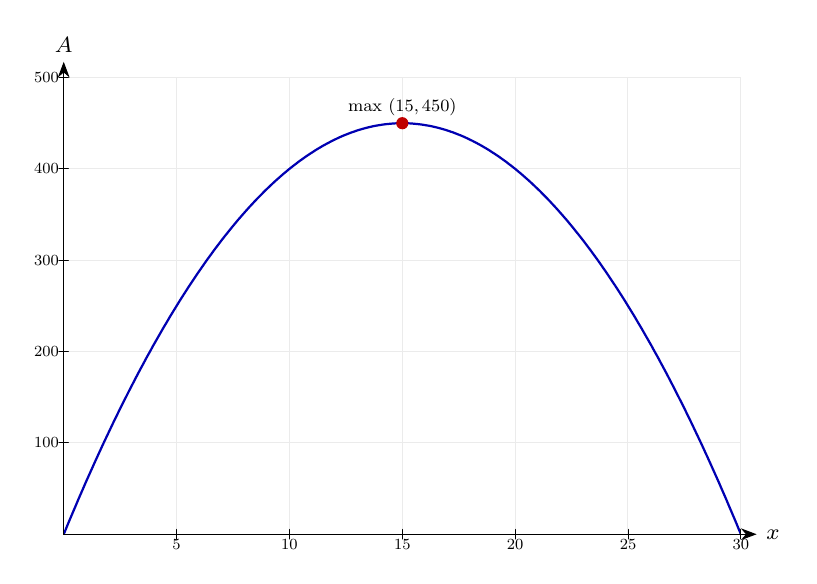
\begin{tikzpicture}[>={Stealth[length=2mm]},font=\footnotesize,line cap=round,line join=round]
\begin{scope}
\clip (0,0) rectangle (8.6,5.8);
\draw[gray!16] (0,0) grid[xstep=1.433,ystep=1.16] (8.6,5.8);
\draw[blue!70!black,thick] (0,0) -- (0.031,0.074) -- (0.061,0.148) -- (0.092,0.221) -- (0.123,0.294) -- (0.154,0.366) -- (0.184,0.438) -- (0.215,0.509) -- (0.246,0.58) -- (0.276,0.65) -- (0.307,0.719) -- (0.338,0.788) -- (0.369,0.857) -- (0.399,0.924) -- (0.43,0.992) -- (0.461,1.059) -- (0.491,1.125) -- (0.522,1.191) -- (0.553,1.256) -- (0.584,1.321) -- (0.614,1.385) -- (0.645,1.449) -- (0.676,1.512) -- (0.706,1.574) -- (0.737,1.636) -- (0.768,1.698) -- (0.799,1.759) -- (0.829,1.819) -- (0.86,1.879) -- (0.891,1.939) -- (0.921,1.997) -- (0.952,2.056) -- (0.983,2.114) -- (1.014,2.171) -- (1.044,2.228) -- (1.075,2.284) -- (1.106,2.339) -- (1.136,2.395) -- (1.167,2.449) -- (1.198,2.503) -- (1.229,2.557) -- (1.259,2.61) -- (1.29,2.662) -- (1.321,2.714) -- (1.351,2.766) -- (1.382,2.816) -- (1.413,2.867) -- (1.444,2.917) -- (1.474,2.966) -- (1.505,3.015) -- (1.536,3.063) -- (1.566,3.11) -- (1.597,3.158) -- (1.628,3.204) -- (1.659,3.25) -- (1.689,3.296) -- (1.72,3.341) -- (1.751,3.385) -- (1.781,3.429) -- (1.812,3.473) -- (1.843,3.516) -- (1.874,3.558) -- (1.904,3.6) -- (1.935,3.641) -- (1.966,3.682) -- (1.996,3.722) -- (2.027,3.762) -- (2.058,3.801) -- (2.089,3.839) -- (2.119,3.877) -- (2.15,3.915) -- (2.181,3.952) -- (2.211,3.989) -- (2.242,4.024) -- (2.273,4.06) -- (2.304,4.095) -- (2.334,4.129) -- (2.365,4.163) -- (2.396,4.196) -- (2.426,4.229) -- (2.457,4.261) -- (2.488,4.293) -- (2.519,4.324) -- (2.549,4.355) -- (2.58,4.385) -- (2.611,4.414) -- (2.641,4.443) -- (2.672,4.472) -- (2.703,4.5) -- (2.734,4.527) -- (2.764,4.554) -- (2.795,4.581) -- (2.826,4.606) -- (2.856,4.632) -- (2.887,4.656) -- (2.918,4.681) -- (2.949,4.704) -- (2.979,4.728) -- (3.01,4.75) -- (3.041,4.772) -- (3.071,4.794) -- (3.102,4.815) -- (3.133,4.835) -- (3.164,4.855) -- (3.194,4.875) -- (3.225,4.894) -- (3.256,4.912) -- (3.286,4.93) -- (3.317,4.947) -- (3.348,4.964) -- (3.379,4.98) -- (3.409,4.996) -- (3.44,5.011) -- (3.471,5.026) -- (3.501,5.04) -- (3.532,5.054) -- (3.563,5.067) -- (3.594,5.079) -- (3.624,5.091) -- (3.655,5.103) -- (3.686,5.113) -- (3.716,5.124) -- (3.747,5.134) -- (3.778,5.143) -- (3.809,5.152) -- (3.839,5.16) -- (3.87,5.168) -- (3.901,5.175) -- (3.931,5.182) -- (3.962,5.188) -- (3.993,5.193) -- (4.024,5.198) -- (4.054,5.203) -- (4.085,5.207) -- (4.116,5.21) -- (4.146,5.213) -- (4.177,5.216) -- (4.208,5.218) -- (4.239,5.219) -- (4.269,5.22) -- (4.3,5.22) -- (4.331,5.22) -- (4.361,5.219) -- (4.392,5.218) -- (4.423,5.216) -- (4.454,5.213) -- (4.484,5.21) -- (4.515,5.207) -- (4.546,5.203) -- (4.576,5.198) -- (4.607,5.193) -- (4.638,5.188) -- (4.669,5.182) -- (4.699,5.175) -- (4.73,5.168) -- (4.761,5.16) -- (4.791,5.152) -- (4.822,5.143) -- (4.853,5.134) -- (4.884,5.124) -- (4.914,5.113) -- (4.945,5.103) -- (4.976,5.091) -- (5.006,5.079) -- (5.037,5.067) -- (5.068,5.054) -- (5.099,5.04) -- (5.129,5.026) -- (5.16,5.011) -- (5.191,4.996) -- (5.221,4.98) -- (5.252,4.964) -- (5.283,4.947) -- (5.314,4.93) -- (5.344,4.912) -- (5.375,4.894) -- (5.406,4.875) -- (5.436,4.855) -- (5.467,4.835) -- (5.498,4.815) -- (5.529,4.794) -- (5.559,4.772) -- (5.59,4.75) -- (5.621,4.728) -- (5.651,4.704) -- (5.682,4.681) -- (5.713,4.656) -- (5.744,4.632) -- (5.774,4.606) -- (5.805,4.581) -- (5.836,4.554) -- (5.866,4.527) -- (5.897,4.5) -- (5.928,4.472) -- (5.959,4.443) -- (5.989,4.414) -- (6.02,4.385) -- (6.051,4.355) -- (6.081,4.324) -- (6.112,4.293) -- (6.143,4.261) -- (6.174,4.229) -- (6.204,4.196) -- (6.235,4.163) -- (6.266,4.129) -- (6.296,4.095) -- (6.327,4.06) -- (6.358,4.024) -- (6.389,3.989) -- (6.419,3.952) -- (6.45,3.915) -- (6.481,3.877) -- (6.511,3.839) -- (6.542,3.801) -- (6.573,3.762) -- (6.604,3.722) -- (6.634,3.682) -- (6.665,3.641) -- (6.696,3.6) -- (6.726,3.558) -- (6.757,3.516) -- (6.788,3.473) -- (6.819,3.429) -- (6.849,3.385) -- (6.88,3.341) -- (6.911,3.296) -- (6.941,3.25) -- (6.972,3.204) -- (7.003,3.158) -- (7.034,3.11) -- (7.064,3.063) -- (7.095,3.015) -- (7.126,2.966) -- (7.156,2.917) -- (7.187,2.867) -- (7.218,2.816) -- (7.249,2.766) -- (7.279,2.714) -- (7.31,2.662) -- (7.341,2.61) -- (7.371,2.557) -- (7.402,2.503) -- (7.433,2.449) -- (7.464,2.395) -- (7.494,2.339) -- (7.525,2.284) -- (7.556,2.228) -- (7.586,2.171) -- (7.617,2.114) -- (7.648,2.056) -- (7.679,1.997) -- (7.709,1.939) -- (7.74,1.879) -- (7.771,1.819) -- (7.801,1.759) -- (7.832,1.698) -- (7.863,1.636) -- (7.894,1.574) -- (7.924,1.512) -- (7.955,1.449) -- (7.986,1.385) -- (8.016,1.321) -- (8.047,1.256) -- (8.078,1.191) -- (8.109,1.125) -- (8.139,1.059) -- (8.17,0.992) -- (8.201,0.924) -- (8.231,0.857) -- (8.262,0.788) -- (8.293,0.719) -- (8.324,0.65) -- (8.354,0.58) -- (8.385,0.509) -- (8.416,0.438) -- (8.446,0.366) -- (8.477,0.294) -- (8.508,0.221) -- (8.539,0.148) -- (8.569,0.074) -- (8.6,0);
\end{scope}
\draw[->] (0,0) -- (8.8,0) node[right]{$x$};
\draw[->] (0,0) -- (0,6) node[above]{$A$};
\draw (1.433,-0.06) -- (1.433,0.06) node[below=1pt,scale=0.7]{$5$};
\draw (2.867,-0.06) -- (2.867,0.06) node[below=1pt,scale=0.7]{$10$};
\draw (4.3,-0.06) -- (4.3,0.06) node[below=1pt,scale=0.7]{$15$};
\draw (5.733,-0.06) -- (5.733,0.06) node[below=1pt,scale=0.7]{$20$};
\draw (7.167,-0.06) -- (7.167,0.06) node[below=1pt,scale=0.7]{$25$};
\draw (8.6,-0.06) -- (8.6,0.06) node[below=1pt,scale=0.7]{$30$};
\draw (-0.06,1.16) -- (0.06,1.16) node[left=1pt,scale=0.7]{$100$};
\draw (-0.06,2.32) -- (0.06,2.32) node[left=1pt,scale=0.7]{$200$};
\draw (-0.06,3.48) -- (0.06,3.48) node[left=1pt,scale=0.7]{$300$};
\draw (-0.06,4.64) -- (0.06,4.64) node[left=1pt,scale=0.7]{$400$};
\draw (-0.06,5.8) -- (0.06,5.8) node[left=1pt,scale=0.7]{$500$};
\fill[red!75!black] (4.3,5.22) circle (2.2pt);
\node[above,scale=0.78] at (4.3,5.22) {max $(15,450)$};
\end{tikzpicture}
}
\end{center}
\small The model plotted against its variable, with the key point(s) marked.\normalsize

\medskip\hrule

\section*{Real-Life Problems 51\quad\small\texttt{(d5-051)}}
\addcontentsline{toc}{section}{Real-Life Problems 51 (d5-051)}
\textit{Difficulty: Standard \quad\textbar\quad Marks: 6}

\question{A piece of wire of length 40 cm is cut into two pieces and each piece is bent into a square. Find the lengths so that the total area enclosed is a minimum.}

\textbf{Worked solution.}

\textit{Step 1: Let the squares have sides \( x \) and \( y \).}
\[\begin{gathered}
4x + 4y = 40 \implies y = 10 - x
\end{gathered}\]
Each square has perimeter \( 4 \times \text{side} \), so the two perimeters sum to 40 cm. Use this to eliminate \( y \).

\textit{Step 2: Total area.}
\[\begin{gathered}
S = x^2 + (10 - x)^2 = 2x^2 - 20x + 100
\end{gathered}\]
Sum the two square areas, then expand \( (10-x)^2 = 100 - 20x + x^2 \).

\textit{Step 3: Differentiate.}
\[\begin{gathered}
\frac{\mathrm{d}S}{\mathrm{d}x} = 4x - 20 = 0 \implies x = 5
\end{gathered}\]
A stationary point of total area. The positive coefficient of \( x^2 \) means \( S \) is an upward parabola, so this stationary point is a minimum (confirmed by \( \dfrac{\mathrm{d}^2 S}{\mathrm{d}x^2} = 4 > 0 \)).

\textit{Step 4: Both pieces equal.}
\[\begin{gathered}
y = 5; \, S = 25 + 25 = 50 \text{ cm}^2
\end{gathered}\]
When the two squares are identical, surface area is minimised. Cut the wire into two equal 20 cm pieces.

\begin{answerbox}
\textbf{Final answer:}\quad Cut into two equal 20 cm pieces; minimum area \(\displaystyle  = 50 \text{ cm}^2 \)
\end{answerbox}
\textbf{Diagram.}

\begin{center}
\resizebox{\ifdim\width>\linewidth \linewidth\else \width\fi}{!}{%
\begin{tikzpicture}[>={Stealth[length=2mm]},font=\footnotesize,line cap=round,line join=round]
\begin{scope}
\clip (0,0) rectangle (8.6,5.8);
\draw[gray!16] (0,0) grid[xstep=1.075,ystep=0.967] (8.6,5.8);
\draw[blue!70!black,thick] (0,4.833) -- (0.031,4.799) -- (0.061,4.765) -- (0.092,4.731) -- (0.123,4.697) -- (0.154,4.664) -- (0.184,4.631) -- (0.215,4.598) -- (0.246,4.565) -- (0.276,4.533) -- (0.307,4.5) -- (0.338,4.468) -- (0.369,4.437) -- (0.399,4.405) -- (0.43,4.374) -- (0.461,4.343) -- (0.491,4.313) -- (0.522,4.282) -- (0.553,4.252) -- (0.584,4.222) -- (0.614,4.192) -- (0.645,4.163) -- (0.676,4.133) -- (0.706,4.105) -- (0.737,4.076) -- (0.768,4.047) -- (0.799,4.019) -- (0.829,3.991) -- (0.86,3.963) -- (0.891,3.936) -- (0.921,3.909) -- (0.952,3.882) -- (0.983,3.855) -- (1.014,3.828) -- (1.044,3.802) -- (1.075,3.776) -- (1.106,3.75) -- (1.136,3.725) -- (1.167,3.699) -- (1.198,3.674) -- (1.229,3.65) -- (1.259,3.625) -- (1.29,3.601) -- (1.321,3.577) -- (1.351,3.553) -- (1.382,3.529) -- (1.413,3.506) -- (1.444,3.483) -- (1.474,3.46) -- (1.505,3.438) -- (1.536,3.415) -- (1.566,3.393) -- (1.597,3.371) -- (1.628,3.35) -- (1.659,3.329) -- (1.689,3.308) -- (1.72,3.287) -- (1.751,3.266) -- (1.781,3.246) -- (1.812,3.226) -- (1.843,3.206) -- (1.874,3.186) -- (1.904,3.167) -- (1.935,3.148) -- (1.966,3.129) -- (1.996,3.11) -- (2.027,3.092) -- (2.058,3.074) -- (2.089,3.056) -- (2.119,3.038) -- (2.15,3.021) -- (2.181,3.004) -- (2.211,2.987) -- (2.242,2.97) -- (2.273,2.954) -- (2.304,2.938) -- (2.334,2.922) -- (2.365,2.906) -- (2.396,2.891) -- (2.426,2.875) -- (2.457,2.861) -- (2.488,2.846) -- (2.519,2.831) -- (2.549,2.817) -- (2.58,2.803) -- (2.611,2.79) -- (2.641,2.776) -- (2.672,2.763) -- (2.703,2.75) -- (2.734,2.737) -- (2.764,2.725) -- (2.795,2.713) -- (2.826,2.701) -- (2.856,2.689) -- (2.887,2.678) -- (2.918,2.666) -- (2.949,2.655) -- (2.979,2.645) -- (3.01,2.634) -- (3.041,2.624) -- (3.071,2.614) -- (3.102,2.604) -- (3.133,2.595) -- (3.164,2.585) -- (3.194,2.576) -- (3.225,2.568) -- (3.256,2.559) -- (3.286,2.551) -- (3.317,2.543) -- (3.348,2.535) -- (3.379,2.528) -- (3.409,2.52) -- (3.44,2.513) -- (3.471,2.507) -- (3.501,2.5) -- (3.532,2.494) -- (3.563,2.488) -- (3.594,2.482) -- (3.624,2.476) -- (3.655,2.471) -- (3.686,2.466) -- (3.716,2.461) -- (3.747,2.457) -- (3.778,2.452) -- (3.809,2.448) -- (3.839,2.444) -- (3.87,2.441) -- (3.901,2.438) -- (3.931,2.434) -- (3.962,2.432) -- (3.993,2.429) -- (4.024,2.427) -- (4.054,2.425) -- (4.085,2.423) -- (4.116,2.421) -- (4.146,2.42) -- (4.177,2.419) -- (4.208,2.418) -- (4.239,2.417) -- (4.269,2.417) -- (4.3,2.417) -- (4.331,2.417) -- (4.361,2.417) -- (4.392,2.418) -- (4.423,2.419) -- (4.454,2.42) -- (4.484,2.421) -- (4.515,2.423) -- (4.546,2.425) -- (4.576,2.427) -- (4.607,2.429) -- (4.638,2.432) -- (4.669,2.434) -- (4.699,2.438) -- (4.73,2.441) -- (4.761,2.444) -- (4.791,2.448) -- (4.822,2.452) -- (4.853,2.457) -- (4.884,2.461) -- (4.914,2.466) -- (4.945,2.471) -- (4.976,2.476) -- (5.006,2.482) -- (5.037,2.488) -- (5.068,2.494) -- (5.099,2.5) -- (5.129,2.507) -- (5.16,2.513) -- (5.191,2.52) -- (5.221,2.528) -- (5.252,2.535) -- (5.283,2.543) -- (5.314,2.551) -- (5.344,2.559) -- (5.375,2.568) -- (5.406,2.576) -- (5.436,2.585) -- (5.467,2.595) -- (5.498,2.604) -- (5.529,2.614) -- (5.559,2.624) -- (5.59,2.634) -- (5.621,2.645) -- (5.651,2.655) -- (5.682,2.666) -- (5.713,2.678) -- (5.744,2.689) -- (5.774,2.701) -- (5.805,2.713) -- (5.836,2.725) -- (5.866,2.737) -- (5.897,2.75) -- (5.928,2.763) -- (5.959,2.776) -- (5.989,2.79) -- (6.02,2.803) -- (6.051,2.817) -- (6.081,2.831) -- (6.112,2.846) -- (6.143,2.861) -- (6.174,2.875) -- (6.204,2.891) -- (6.235,2.906) -- (6.266,2.922) -- (6.296,2.938) -- (6.327,2.954) -- (6.358,2.97) -- (6.389,2.987) -- (6.419,3.004) -- (6.45,3.021) -- (6.481,3.038) -- (6.511,3.056) -- (6.542,3.074) -- (6.573,3.092) -- (6.604,3.11) -- (6.634,3.129) -- (6.665,3.148) -- (6.696,3.167) -- (6.726,3.186) -- (6.757,3.206) -- (6.788,3.226) -- (6.819,3.246) -- (6.849,3.266) -- (6.88,3.287) -- (6.911,3.308) -- (6.941,3.329) -- (6.972,3.35) -- (7.003,3.371) -- (7.034,3.393) -- (7.064,3.415) -- (7.095,3.438) -- (7.126,3.46) -- (7.156,3.483) -- (7.187,3.506) -- (7.218,3.529) -- (7.249,3.553) -- (7.279,3.577) -- (7.31,3.601) -- (7.341,3.625) -- (7.371,3.65) -- (7.402,3.674) -- (7.433,3.699) -- (7.464,3.725) -- (7.494,3.75) -- (7.525,3.776) -- (7.556,3.802) -- (7.586,3.828) -- (7.617,3.855) -- (7.648,3.882) -- (7.679,3.909) -- (7.709,3.936) -- (7.74,3.963) -- (7.771,3.991) -- (7.801,4.019) -- (7.832,4.047) -- (7.863,4.076) -- (7.894,4.105) -- (7.924,4.133) -- (7.955,4.163) -- (7.986,4.192) -- (8.016,4.222) -- (8.047,4.252) -- (8.078,4.282) -- (8.109,4.313) -- (8.139,4.343) -- (8.17,4.374) -- (8.201,4.405) -- (8.231,4.437) -- (8.262,4.468) -- (8.293,4.5) -- (8.324,4.533) -- (8.354,4.565) -- (8.385,4.598) -- (8.416,4.631) -- (8.446,4.664) -- (8.477,4.697) -- (8.508,4.731) -- (8.539,4.765) -- (8.569,4.799) -- (8.6,4.833);
\end{scope}
\draw[->] (0,0) -- (8.8,0) node[right]{$x$};
\draw[->] (0,0) -- (0,6) node[above]{$A$};
\draw (1.075,-0.06) -- (1.075,0.06) node[below=1pt,scale=0.7]{$5$};
\draw (2.15,-0.06) -- (2.15,0.06) node[below=1pt,scale=0.7]{$10$};
\draw (3.225,-0.06) -- (3.225,0.06) node[below=1pt,scale=0.7]{$15$};
\draw (4.3,-0.06) -- (4.3,0.06) node[below=1pt,scale=0.7]{$20$};
\draw (5.375,-0.06) -- (5.375,0.06) node[below=1pt,scale=0.7]{$25$};
\draw (6.45,-0.06) -- (6.45,0.06) node[below=1pt,scale=0.7]{$30$};
\draw (7.525,-0.06) -- (7.525,0.06) node[below=1pt,scale=0.7]{$35$};
\draw (8.6,-0.06) -- (8.6,0.06) node[below=1pt,scale=0.7]{$40$};
\draw (-0.06,0.967) -- (0.06,0.967) node[left=1pt,scale=0.7]{$20$};
\draw (-0.06,1.933) -- (0.06,1.933) node[left=1pt,scale=0.7]{$40$};
\draw (-0.06,2.9) -- (0.06,2.9) node[left=1pt,scale=0.7]{$60$};
\draw (-0.06,3.867) -- (0.06,3.867) node[left=1pt,scale=0.7]{$80$};
\draw (-0.06,4.833) -- (0.06,4.833) node[left=1pt,scale=0.7]{$100$};
\draw (-0.06,5.8) -- (0.06,5.8) node[left=1pt,scale=0.7]{$120$};
\fill[red!75!black] (4.3,2.417) circle (2.2pt);
\node[above,scale=0.78] at (4.3,2.417) {min $(20,50)$};
\end{tikzpicture}
}
\end{center}
\small The model plotted against its variable, with the key point(s) marked.\normalsize

\medskip\hrule

\section*{Real-Life Problems 52\quad\small\texttt{(d5-052)}}
\addcontentsline{toc}{section}{Real-Life Problems 52 (d5-052)}
\textit{Difficulty: Foundation \quad\textbar\quad Marks: 4}

\question{The power output of an engine is modelled by \( P = 120t - 3t^2 \) watts, where \( t \) is in seconds. Find the time at which the power is greatest and the maximum power.}

\textbf{Worked solution.}

\textit{Step 1: Differentiate.}
\[\begin{gathered}
\frac{\mathrm{d}P}{\mathrm{d}t} = 120 - 6t
\end{gathered}\]
Power output is greatest when its rate of change is zero, so we will need \( \dfrac{\mathrm{d}P}{\mathrm{d}t} = 0 \).

\textit{Step 2: Set to zero.}
\[\begin{gathered}
120 - 6t = 0 \implies t = 20
\end{gathered}\]
The negative coefficient of \( t^2 \) means \( P \) is a downward parabola, so this stationary point is the maximum.

\textit{Step 3: Maximum.}
\[\begin{gathered}
P = 120(20) - 3(400) = 2400 - 1200 = 1200 \text{ W}
\end{gathered}\]
Substitute \( t = 20 \) into the original power expression.

\begin{answerbox}
\textbf{Final answer:}\quad \(\displaystyle  t = 20 \) s, \(\displaystyle  P_{\max} = 1200 \) W
\end{answerbox}
\textbf{Diagram.}

\begin{center}
\resizebox{\ifdim\width>\linewidth \linewidth\else \width\fi}{!}{%
\begin{tikzpicture}[>={Stealth[length=2mm]},font=\footnotesize,line cap=round,line join=round]
\begin{scope}
\clip (0,0) rectangle (8.6,5.8);
\draw[gray!16] (0,0) grid[xstep=1.075,ystep=0.829] (8.6,5.8);
\draw[blue!70!black,thick] (0,0) -- (0.031,0.071) -- (0.061,0.141) -- (0.092,0.211) -- (0.123,0.28) -- (0.154,0.349) -- (0.184,0.417) -- (0.215,0.485) -- (0.246,0.552) -- (0.276,0.619) -- (0.307,0.685) -- (0.338,0.751) -- (0.369,0.816) -- (0.399,0.88) -- (0.43,0.945) -- (0.461,1.008) -- (0.491,1.071) -- (0.522,1.134) -- (0.553,1.196) -- (0.584,1.258) -- (0.614,1.319) -- (0.645,1.38) -- (0.676,1.44) -- (0.706,1.499) -- (0.737,1.558) -- (0.768,1.617) -- (0.799,1.675) -- (0.829,1.733) -- (0.86,1.79) -- (0.891,1.846) -- (0.921,1.902) -- (0.952,1.958) -- (0.983,2.013) -- (1.014,2.067) -- (1.044,2.121) -- (1.075,2.175) -- (1.106,2.228) -- (1.136,2.281) -- (1.167,2.333) -- (1.198,2.384) -- (1.229,2.435) -- (1.259,2.485) -- (1.29,2.535) -- (1.321,2.585) -- (1.351,2.634) -- (1.382,2.682) -- (1.413,2.73) -- (1.444,2.778) -- (1.474,2.825) -- (1.505,2.871) -- (1.536,2.917) -- (1.566,2.962) -- (1.597,3.007) -- (1.628,3.052) -- (1.659,3.095) -- (1.689,3.139) -- (1.72,3.182) -- (1.751,3.224) -- (1.781,3.266) -- (1.812,3.307) -- (1.843,3.348) -- (1.874,3.388) -- (1.904,3.428) -- (1.935,3.468) -- (1.966,3.506) -- (1.996,3.545) -- (2.027,3.582) -- (2.058,3.62) -- (2.089,3.657) -- (2.119,3.693) -- (2.15,3.729) -- (2.181,3.764) -- (2.211,3.799) -- (2.242,3.833) -- (2.273,3.867) -- (2.304,3.9) -- (2.334,3.933) -- (2.365,3.965) -- (2.396,3.996) -- (2.426,4.028) -- (2.457,4.058) -- (2.488,4.088) -- (2.519,4.118) -- (2.549,4.147) -- (2.58,4.176) -- (2.611,4.204) -- (2.641,4.232) -- (2.672,4.259) -- (2.703,4.286) -- (2.734,4.312) -- (2.764,4.337) -- (2.795,4.362) -- (2.826,4.387) -- (2.856,4.411) -- (2.887,4.435) -- (2.918,4.458) -- (2.949,4.48) -- (2.979,4.502) -- (3.01,4.524) -- (3.041,4.545) -- (3.071,4.566) -- (3.102,4.586) -- (3.133,4.605) -- (3.164,4.624) -- (3.194,4.643) -- (3.225,4.661) -- (3.256,4.678) -- (3.286,4.695) -- (3.317,4.712) -- (3.348,4.728) -- (3.379,4.743) -- (3.409,4.758) -- (3.44,4.773) -- (3.471,4.787) -- (3.501,4.8) -- (3.532,4.813) -- (3.563,4.825) -- (3.594,4.837) -- (3.624,4.849) -- (3.655,4.86) -- (3.686,4.87) -- (3.716,4.88) -- (3.747,4.889) -- (3.778,4.898) -- (3.809,4.906) -- (3.839,4.914) -- (3.87,4.922) -- (3.901,4.929) -- (3.931,4.935) -- (3.962,4.941) -- (3.993,4.946) -- (4.024,4.951) -- (4.054,4.955) -- (4.085,4.959) -- (4.116,4.962) -- (4.146,4.965) -- (4.177,4.967) -- (4.208,4.969) -- (4.239,4.97) -- (4.269,4.971) -- (4.3,4.971) -- (4.331,4.971) -- (4.361,4.97) -- (4.392,4.969) -- (4.423,4.967) -- (4.454,4.965) -- (4.484,4.962) -- (4.515,4.959) -- (4.546,4.955) -- (4.576,4.951) -- (4.607,4.946) -- (4.638,4.941) -- (4.669,4.935) -- (4.699,4.929) -- (4.73,4.922) -- (4.761,4.914) -- (4.791,4.906) -- (4.822,4.898) -- (4.853,4.889) -- (4.884,4.88) -- (4.914,4.87) -- (4.945,4.86) -- (4.976,4.849) -- (5.006,4.837) -- (5.037,4.825) -- (5.068,4.813) -- (5.099,4.8) -- (5.129,4.787) -- (5.16,4.773) -- (5.191,4.758) -- (5.221,4.743) -- (5.252,4.728) -- (5.283,4.712) -- (5.314,4.695) -- (5.344,4.678) -- (5.375,4.661) -- (5.406,4.643) -- (5.436,4.624) -- (5.467,4.605) -- (5.498,4.586) -- (5.529,4.566) -- (5.559,4.545) -- (5.59,4.524) -- (5.621,4.502) -- (5.651,4.48) -- (5.682,4.458) -- (5.713,4.435) -- (5.744,4.411) -- (5.774,4.387) -- (5.805,4.362) -- (5.836,4.337) -- (5.866,4.312) -- (5.897,4.286) -- (5.928,4.259) -- (5.959,4.232) -- (5.989,4.204) -- (6.02,4.176) -- (6.051,4.147) -- (6.081,4.118) -- (6.112,4.088) -- (6.143,4.058) -- (6.174,4.028) -- (6.204,3.996) -- (6.235,3.965) -- (6.266,3.933) -- (6.296,3.9) -- (6.327,3.867) -- (6.358,3.833) -- (6.389,3.799) -- (6.419,3.764) -- (6.45,3.729) -- (6.481,3.693) -- (6.511,3.657) -- (6.542,3.62) -- (6.573,3.582) -- (6.604,3.545) -- (6.634,3.506) -- (6.665,3.468) -- (6.696,3.428) -- (6.726,3.388) -- (6.757,3.348) -- (6.788,3.307) -- (6.819,3.266) -- (6.849,3.224) -- (6.88,3.182) -- (6.911,3.139) -- (6.941,3.095) -- (6.972,3.052) -- (7.003,3.007) -- (7.034,2.962) -- (7.064,2.917) -- (7.095,2.871) -- (7.126,2.825) -- (7.156,2.778) -- (7.187,2.73) -- (7.218,2.682) -- (7.249,2.634) -- (7.279,2.585) -- (7.31,2.535) -- (7.341,2.485) -- (7.371,2.435) -- (7.402,2.384) -- (7.433,2.333) -- (7.464,2.281) -- (7.494,2.228) -- (7.525,2.175) -- (7.556,2.121) -- (7.586,2.067) -- (7.617,2.013) -- (7.648,1.958) -- (7.679,1.902) -- (7.709,1.846) -- (7.74,1.79) -- (7.771,1.733) -- (7.801,1.675) -- (7.832,1.617) -- (7.863,1.558) -- (7.894,1.499) -- (7.924,1.44) -- (7.955,1.38) -- (7.986,1.319) -- (8.016,1.258) -- (8.047,1.196) -- (8.078,1.134) -- (8.109,1.071) -- (8.139,1.008) -- (8.17,0.945) -- (8.201,0.88) -- (8.231,0.816) -- (8.262,0.751) -- (8.293,0.685) -- (8.324,0.619) -- (8.354,0.552) -- (8.385,0.485) -- (8.416,0.417) -- (8.446,0.349) -- (8.477,0.28) -- (8.508,0.211) -- (8.539,0.141) -- (8.569,0.071) -- (8.6,0);
\end{scope}
\draw[->] (0,0) -- (8.8,0) node[right]{$t$};
\draw[->] (0,0) -- (0,6) node[above]{$P$};
\draw (1.075,-0.06) -- (1.075,0.06) node[below=1pt,scale=0.7]{$5$};
\draw (2.15,-0.06) -- (2.15,0.06) node[below=1pt,scale=0.7]{$10$};
\draw (3.225,-0.06) -- (3.225,0.06) node[below=1pt,scale=0.7]{$15$};
\draw (4.3,-0.06) -- (4.3,0.06) node[below=1pt,scale=0.7]{$20$};
\draw (5.375,-0.06) -- (5.375,0.06) node[below=1pt,scale=0.7]{$25$};
\draw (6.45,-0.06) -- (6.45,0.06) node[below=1pt,scale=0.7]{$30$};
\draw (7.525,-0.06) -- (7.525,0.06) node[below=1pt,scale=0.7]{$35$};
\draw (8.6,-0.06) -- (8.6,0.06) node[below=1pt,scale=0.7]{$40$};
\draw (-0.06,0.829) -- (0.06,0.829) node[left=1pt,scale=0.7]{$200$};
\draw (-0.06,1.657) -- (0.06,1.657) node[left=1pt,scale=0.7]{$400$};
\draw (-0.06,2.486) -- (0.06,2.486) node[left=1pt,scale=0.7]{$600$};
\draw (-0.06,3.314) -- (0.06,3.314) node[left=1pt,scale=0.7]{$800$};
\draw (-0.06,4.143) -- (0.06,4.143) node[left=1pt,scale=0.7]{$1000$};
\draw (-0.06,4.971) -- (0.06,4.971) node[left=1pt,scale=0.7]{$1200$};
\draw (-0.06,5.8) -- (0.06,5.8) node[left=1pt,scale=0.7]{$1400$};
\fill[red!75!black] (4.3,4.971) circle (2.2pt);
\node[above,scale=0.78] at (4.3,4.971) {max $(20,1200)$};
\end{tikzpicture}
}
\end{center}
\small The model plotted against its variable, with the key point(s) marked.\normalsize

\medskip\hrule

\section*{Real-Life Problems 53\quad\small\texttt{(d5-053)}}
\addcontentsline{toc}{section}{Real-Life Problems 53 (d5-053)}
\textit{Difficulty: Foundation \quad\textbar\quad Marks: 4}

\question{A tank is being drained. The volume after \( t \) seconds is \( V = 400 - 20t + \dfrac{t^2}{4} \) litres. Find the rate at which the volume is changing at \( t = 10 \) s, and interpret the sign.}

\textbf{Worked solution.}

\textit{Step 1: Differentiate.}
\[\begin{gathered}
\frac{\mathrm{d}V}{\mathrm{d}t} = -20 + \frac{t}{2}
\end{gathered}\]
\( \dfrac{\mathrm{d}V}{\mathrm{d}t} \) is the instantaneous flow rate. Apply the power rule to each term.

\textit{Step 2: Substitute.}
\[\begin{gathered}
\frac{\mathrm{d}V}{\mathrm{d}t}\bigg|_{t=10} = -20 + 5 = -15
\end{gathered}\]
The vertical bar notation evaluates the derivative at \( t = 10 \).

\textit{Step 3: Interpret.}
\[\begin{gathered}
\text{Negative} \Rightarrow \text{volume decreasing}
\end{gathered}\]
A negative rate of change means the volume is shrinking --- the tank is draining at 15 litres per second at this instant.

\begin{answerbox}
\textbf{Final answer:}\quad \(\displaystyle  -15 \) L/s; the tank is draining at 15 litres per second
\end{answerbox}
\textbf{Diagram.}

\begin{center}
\resizebox{\ifdim\width>\linewidth \linewidth\else \width\fi}{!}{%
\begin{tikzpicture}[>={Stealth[length=2mm]},font=\footnotesize,line cap=round,line join=round]
\begin{scope}
\clip (0,0) rectangle (8.6,5.8);
\draw[gray!16] (0,0) grid[xstep=1.075,ystep=1.289] (8.6,5.8);
\draw[orange!85!black,thick,dashed] (0,4.833) -- (8.6,-2.9);
\draw[blue!70!black,thick] (0,5.156) -- (0.031,5.119) -- (0.061,5.082) -- (0.092,5.046) -- (0.123,5.009) -- (0.154,4.973) -- (0.184,4.937) -- (0.215,4.901) -- (0.246,4.865) -- (0.276,4.829) -- (0.307,4.794) -- (0.338,4.758) -- (0.369,4.723) -- (0.399,4.688) -- (0.43,4.653) -- (0.461,4.618) -- (0.491,4.583) -- (0.522,4.549) -- (0.553,4.514) -- (0.584,4.48) -- (0.614,4.445) -- (0.645,4.411) -- (0.676,4.377) -- (0.706,4.343) -- (0.737,4.31) -- (0.768,4.276) -- (0.799,4.243) -- (0.829,4.209) -- (0.86,4.176) -- (0.891,4.143) -- (0.921,4.11) -- (0.952,4.077) -- (0.983,4.044) -- (1.014,4.012) -- (1.044,3.98) -- (1.075,3.947) -- (1.106,3.915) -- (1.136,3.883) -- (1.167,3.851) -- (1.198,3.819) -- (1.229,3.788) -- (1.259,3.756) -- (1.29,3.725) -- (1.321,3.694) -- (1.351,3.663) -- (1.382,3.632) -- (1.413,3.601) -- (1.444,3.57) -- (1.474,3.539) -- (1.505,3.509) -- (1.536,3.479) -- (1.566,3.449) -- (1.597,3.418) -- (1.628,3.389) -- (1.659,3.359) -- (1.689,3.329) -- (1.72,3.3) -- (1.751,3.27) -- (1.781,3.241) -- (1.812,3.212) -- (1.843,3.183) -- (1.874,3.154) -- (1.904,3.125) -- (1.935,3.097) -- (1.966,3.068) -- (1.996,3.04) -- (2.027,3.012) -- (2.058,2.983) -- (2.089,2.956) -- (2.119,2.928) -- (2.15,2.9) -- (2.181,2.872) -- (2.211,2.845) -- (2.242,2.818) -- (2.273,2.791) -- (2.304,2.764) -- (2.334,2.737) -- (2.365,2.71) -- (2.396,2.683) -- (2.426,2.657) -- (2.457,2.63) -- (2.488,2.604) -- (2.519,2.578) -- (2.549,2.552) -- (2.58,2.526) -- (2.611,2.501) -- (2.641,2.475) -- (2.672,2.449) -- (2.703,2.424) -- (2.734,2.399) -- (2.764,2.374) -- (2.795,2.349) -- (2.826,2.324) -- (2.856,2.3) -- (2.887,2.275) -- (2.918,2.251) -- (2.949,2.226) -- (2.979,2.202) -- (3.01,2.178) -- (3.041,2.154) -- (3.071,2.131) -- (3.102,2.107) -- (3.133,2.084) -- (3.164,2.06) -- (3.194,2.037) -- (3.225,2.014) -- (3.256,1.991) -- (3.286,1.968) -- (3.317,1.945) -- (3.348,1.923) -- (3.379,1.9) -- (3.409,1.878) -- (3.44,1.856) -- (3.471,1.834) -- (3.501,1.812) -- (3.532,1.79) -- (3.563,1.769) -- (3.594,1.747) -- (3.624,1.726) -- (3.655,1.705) -- (3.686,1.683) -- (3.716,1.662) -- (3.747,1.642) -- (3.778,1.621) -- (3.809,1.6) -- (3.839,1.58) -- (3.87,1.56) -- (3.901,1.539) -- (3.931,1.519) -- (3.962,1.499) -- (3.993,1.48) -- (4.024,1.46) -- (4.054,1.44) -- (4.085,1.421) -- (4.116,1.402) -- (4.146,1.383) -- (4.177,1.364) -- (4.208,1.345) -- (4.239,1.326) -- (4.269,1.307) -- (4.3,1.289) -- (4.331,1.271) -- (4.361,1.252) -- (4.392,1.234) -- (4.423,1.216) -- (4.454,1.198) -- (4.484,1.181) -- (4.515,1.163) -- (4.546,1.146) -- (4.576,1.129) -- (4.607,1.111) -- (4.638,1.094) -- (4.669,1.077) -- (4.699,1.061) -- (4.73,1.044) -- (4.761,1.027) -- (4.791,1.011) -- (4.822,0.995) -- (4.853,0.979) -- (4.884,0.963) -- (4.914,0.947) -- (4.945,0.931) -- (4.976,0.916) -- (5.006,0.9) -- (5.037,0.885) -- (5.068,0.87) -- (5.099,0.855) -- (5.129,0.84) -- (5.16,0.825) -- (5.191,0.81) -- (5.221,0.796) -- (5.252,0.781) -- (5.283,0.767) -- (5.314,0.753) -- (5.344,0.739) -- (5.375,0.725) -- (5.406,0.711) -- (5.436,0.698) -- (5.467,0.684) -- (5.498,0.671) -- (5.529,0.658) -- (5.559,0.645) -- (5.59,0.632) -- (5.621,0.619) -- (5.651,0.606) -- (5.682,0.593) -- (5.713,0.581) -- (5.744,0.569) -- (5.774,0.557) -- (5.805,0.545) -- (5.836,0.533) -- (5.866,0.521) -- (5.897,0.509) -- (5.928,0.498) -- (5.959,0.486) -- (5.989,0.475) -- (6.02,0.464) -- (6.051,0.453) -- (6.081,0.442) -- (6.112,0.431) -- (6.143,0.421) -- (6.174,0.41) -- (6.204,0.4) -- (6.235,0.39) -- (6.266,0.38) -- (6.296,0.37) -- (6.327,0.36) -- (6.358,0.35) -- (6.389,0.341) -- (6.419,0.331) -- (6.45,0.322) -- (6.481,0.313) -- (6.511,0.304) -- (6.542,0.295) -- (6.573,0.286) -- (6.604,0.278) -- (6.634,0.269) -- (6.665,0.261) -- (6.696,0.253) -- (6.726,0.245) -- (6.757,0.237) -- (6.788,0.229) -- (6.819,0.221) -- (6.849,0.214) -- (6.88,0.206) -- (6.911,0.199) -- (6.941,0.192) -- (6.972,0.185) -- (7.003,0.178) -- (7.034,0.171) -- (7.064,0.164) -- (7.095,0.158) -- (7.126,0.152) -- (7.156,0.145) -- (7.187,0.139) -- (7.218,0.133) -- (7.249,0.127) -- (7.279,0.122) -- (7.31,0.116) -- (7.341,0.111) -- (7.371,0.105) -- (7.402,0.1) -- (7.433,0.095) -- (7.464,0.09) -- (7.494,0.085) -- (7.525,0.081) -- (7.556,0.076) -- (7.586,0.072) -- (7.617,0.067) -- (7.648,0.063) -- (7.679,0.059) -- (7.709,0.055) -- (7.74,0.052) -- (7.771,0.048) -- (7.801,0.044) -- (7.832,0.041) -- (7.863,0.038) -- (7.894,0.035) -- (7.924,0.032) -- (7.955,0.029) -- (7.986,0.026) -- (8.016,0.024) -- (8.047,0.021) -- (8.078,0.019) -- (8.109,0.017) -- (8.139,0.015) -- (8.17,0.013) -- (8.201,0.011) -- (8.231,0.009) -- (8.262,0.008) -- (8.293,0.007) -- (8.324,0.005) -- (8.354,0.004) -- (8.385,0.003) -- (8.416,0.002) -- (8.446,0.002) -- (8.477,0.001) -- (8.508,0.001) -- (8.539,0) -- (8.569,0) -- (8.6,0);
\end{scope}
\draw[->] (0,0) -- (8.8,0) node[right]{$t$};
\draw[->] (0,0) -- (0,6) node[above]{$V$};
\draw (1.075,-0.06) -- (1.075,0.06) node[below=1pt,scale=0.7]{$5$};
\draw (2.15,-0.06) -- (2.15,0.06) node[below=1pt,scale=0.7]{$10$};
\draw (3.225,-0.06) -- (3.225,0.06) node[below=1pt,scale=0.7]{$15$};
\draw (4.3,-0.06) -- (4.3,0.06) node[below=1pt,scale=0.7]{$20$};
\draw (5.375,-0.06) -- (5.375,0.06) node[below=1pt,scale=0.7]{$25$};
\draw (6.45,-0.06) -- (6.45,0.06) node[below=1pt,scale=0.7]{$30$};
\draw (7.525,-0.06) -- (7.525,0.06) node[below=1pt,scale=0.7]{$35$};
\draw (8.6,-0.06) -- (8.6,0.06) node[below=1pt,scale=0.7]{$40$};
\draw (-0.06,1.289) -- (0.06,1.289) node[left=1pt,scale=0.7]{$100$};
\draw (-0.06,2.578) -- (0.06,2.578) node[left=1pt,scale=0.7]{$200$};
\draw (-0.06,3.867) -- (0.06,3.867) node[left=1pt,scale=0.7]{$300$};
\draw (-0.06,5.156) -- (0.06,5.156) node[left=1pt,scale=0.7]{$400$};
\fill[red!75!black] (2.15,2.9) circle (2.2pt);
\node[above right,scale=0.78] at (2.15,2.9) {$t{=}10$};
\end{tikzpicture}
}
\end{center}
\small The model plotted against its variable, with the key point(s) marked and the tangent (dashed) showing the instantaneous rate.\normalsize

\medskip\hrule

\section*{Real-Life Problems 54\quad\small\texttt{(d5-054)}}
\addcontentsline{toc}{section}{Real-Life Problems 54 (d5-054)}
\textit{Difficulty: Standard \quad\textbar\quad Marks: 8}

\question{A closed rectangular box has a square base of side \( x \) cm, height \( h \) cm and volume \( 27 \) cm\(^3\). (a) Show that the surface area is \( S = 2x^2 + \dfrac{108}{x} \). (b) Find the value of \( x \) that minimises \( S \), and find the minimum surface area.}

\textbf{Worked solution.}

\textit{Step 1: (a) Volume.}
\[\begin{gathered}
x^2 h = 27 \implies h = \frac{27}{x^2}
\end{gathered}\]
Fixed volume relates \( h \) to \( x \). Use this to eliminate \( h \) from the surface area so only one variable remains.

\textit{Step 2: Surface area: 2 squares + 4 sides.}
\[\begin{gathered}
S = 2x^2 + 4xh = 2x^2 + \frac{108}{x} \, \checkmark
\end{gathered}\]
Two square ends contribute \( 2x^2 \); the four rectangular sides each have area \( xh \). Substitute \( h = 27/x^2 \) and simplify.

\textit{Step 3: (b) Differentiate.}
\[\begin{gathered}
\frac{\mathrm{d}S}{\mathrm{d}x} = 4x - \frac{108}{x^2}
\end{gathered}\]
Rewrite \( \dfrac{108}{x} \) as \( 108x^{-1} \) before applying the power rule.

\textit{Step 4: Set to zero.}
\[\begin{gathered}
4x = \frac{108}{x^2} \implies x^3 = 27 \implies x = 3
\end{gathered}\]
The optimal base width is where the derivative vanishes. Multiply by \( x^2 \) and divide by 4 to isolate \( x^3 \).

\textit{Step 5: Minimum surface area.}
\[\begin{gathered}
S = 2(9) + \frac{108}{3} = 18 + 36 = 54 \text{ cm}^2
\end{gathered}\]
Substitute \( x = 3 \). A check of \( \dfrac{\mathrm{d}^2 S}{\mathrm{d}x^2} = 4 + 216/x^3 > 0 \) confirms a minimum.

\begin{answerbox}
\textbf{Final answer:}\quad (a) Shown. \\[3pt]  (b) \(\displaystyle  x = 3 \) cm; \(\displaystyle  S_{\min} = 54 \text{ cm}^2 \)
\end{answerbox}
\textbf{Diagram.}

\begin{center}
\resizebox{\ifdim\width>\linewidth \linewidth\else \width\fi}{!}{%
\begin{tikzpicture}[>={Stealth[length=2mm]},font=\footnotesize,line cap=round,line join=round]
\begin{scope}
\clip (0,0) rectangle (8.6,5.8);
\draw[gray!16] (0,0) grid[xstep=1.433,ystep=0.773] (8.6,5.8);
\draw[blue!70!black,thick] (0.031,11.6) -- (0.061,11.6) -- (0.092,11.6) -- (0.123,11.6) -- (0.154,11.6) -- (0.184,11.6) -- (0.215,11.6) -- (0.246,11.6) -- (0.276,11.6) -- (0.307,11.6) -- (0.338,11.6) -- (0.369,11.6) -- (0.399,11.6) -- (0.43,11.6) -- (0.461,11.6) -- (0.491,11.6) -- (0.522,11.474) -- (0.553,10.838) -- (0.584,10.27) -- (0.614,9.758) -- (0.645,9.296) -- (0.676,8.875) -- (0.706,8.492) -- (0.737,8.14) -- (0.768,7.817) -- (0.799,7.519) -- (0.829,7.244) -- (0.86,6.988) -- (0.891,6.75) -- (0.921,6.528) -- (0.952,6.321) -- (0.983,6.126) -- (1.014,5.944) -- (1.044,5.773) -- (1.075,5.612) -- (1.106,5.459) -- (1.136,5.316) -- (1.167,5.18) -- (1.198,5.051) -- (1.229,4.929) -- (1.259,4.813) -- (1.29,4.703) -- (1.321,4.598) -- (1.351,4.498) -- (1.382,4.403) -- (1.413,4.312) -- (1.444,4.225) -- (1.474,4.142) -- (1.505,4.062) -- (1.536,3.986) -- (1.566,3.914) -- (1.597,3.844) -- (1.628,3.777) -- (1.659,3.712) -- (1.689,3.651) -- (1.72,3.591) -- (1.751,3.534) -- (1.781,3.479) -- (1.812,3.427) -- (1.843,3.376) -- (1.874,3.327) -- (1.904,3.28) -- (1.935,3.234) -- (1.966,3.19) -- (1.996,3.148) -- (2.027,3.107) -- (2.058,3.068) -- (2.089,3.03) -- (2.119,2.993) -- (2.15,2.958) -- (2.181,2.924) -- (2.211,2.891) -- (2.242,2.859) -- (2.273,2.828) -- (2.304,2.798) -- (2.334,2.769) -- (2.365,2.741) -- (2.396,2.715) -- (2.426,2.688) -- (2.457,2.663) -- (2.488,2.639) -- (2.519,2.615) -- (2.549,2.593) -- (2.58,2.571) -- (2.611,2.549) -- (2.641,2.529) -- (2.672,2.509) -- (2.703,2.49) -- (2.734,2.471) -- (2.764,2.453) -- (2.795,2.436) -- (2.826,2.419) -- (2.856,2.403) -- (2.887,2.387) -- (2.918,2.372) -- (2.949,2.357) -- (2.979,2.343) -- (3.01,2.33) -- (3.041,2.317) -- (3.071,2.304) -- (3.102,2.292) -- (3.133,2.28) -- (3.164,2.269) -- (3.194,2.258) -- (3.225,2.248) -- (3.256,2.237) -- (3.286,2.228) -- (3.317,2.219) -- (3.348,2.21) -- (3.379,2.201) -- (3.409,2.193) -- (3.44,2.185) -- (3.471,2.178) -- (3.501,2.171) -- (3.532,2.164) -- (3.563,2.158) -- (3.594,2.152) -- (3.624,2.146) -- (3.655,2.141) -- (3.686,2.135) -- (3.716,2.13) -- (3.747,2.126) -- (3.778,2.122) -- (3.809,2.118) -- (3.839,2.114) -- (3.87,2.11) -- (3.901,2.107) -- (3.931,2.104) -- (3.962,2.102) -- (3.993,2.099) -- (4.024,2.097) -- (4.054,2.095) -- (4.085,2.093) -- (4.116,2.092) -- (4.146,2.091) -- (4.177,2.09) -- (4.208,2.089) -- (4.239,2.088) -- (4.269,2.088) -- (4.3,2.088) -- (4.331,2.088) -- (4.361,2.088) -- (4.392,2.089) -- (4.423,2.09) -- (4.454,2.091) -- (4.484,2.092) -- (4.515,2.093) -- (4.546,2.095) -- (4.576,2.096) -- (4.607,2.098) -- (4.638,2.1) -- (4.669,2.103) -- (4.699,2.105) -- (4.73,2.108) -- (4.761,2.11) -- (4.791,2.113) -- (4.822,2.117) -- (4.853,2.12) -- (4.884,2.123) -- (4.914,2.127) -- (4.945,2.131) -- (4.976,2.135) -- (5.006,2.139) -- (5.037,2.143) -- (5.068,2.148) -- (5.099,2.152) -- (5.129,2.157) -- (5.16,2.162) -- (5.191,2.167) -- (5.221,2.173) -- (5.252,2.178) -- (5.283,2.184) -- (5.314,2.189) -- (5.344,2.195) -- (5.375,2.201) -- (5.406,2.207) -- (5.436,2.214) -- (5.467,2.22) -- (5.498,2.226) -- (5.529,2.233) -- (5.559,2.24) -- (5.59,2.247) -- (5.621,2.254) -- (5.651,2.261) -- (5.682,2.269) -- (5.713,2.276) -- (5.744,2.284) -- (5.774,2.292) -- (5.805,2.3) -- (5.836,2.308) -- (5.866,2.316) -- (5.897,2.324) -- (5.928,2.332) -- (5.959,2.341) -- (5.989,2.35) -- (6.02,2.358) -- (6.051,2.367) -- (6.081,2.376) -- (6.112,2.386) -- (6.143,2.395) -- (6.174,2.404) -- (6.204,2.414) -- (6.235,2.423) -- (6.266,2.433) -- (6.296,2.443) -- (6.327,2.453) -- (6.358,2.463) -- (6.389,2.473) -- (6.419,2.484) -- (6.45,2.494) -- (6.481,2.505) -- (6.511,2.515) -- (6.542,2.526) -- (6.573,2.537) -- (6.604,2.548) -- (6.634,2.559) -- (6.665,2.57) -- (6.696,2.582) -- (6.726,2.593) -- (6.757,2.605) -- (6.788,2.616) -- (6.819,2.628) -- (6.849,2.64) -- (6.88,2.652) -- (6.911,2.664) -- (6.941,2.676) -- (6.972,2.688) -- (7.003,2.701) -- (7.034,2.713) -- (7.064,2.726) -- (7.095,2.738) -- (7.126,2.751) -- (7.156,2.764) -- (7.187,2.777) -- (7.218,2.79) -- (7.249,2.804) -- (7.279,2.817) -- (7.31,2.83) -- (7.341,2.844) -- (7.371,2.857) -- (7.402,2.871) -- (7.433,2.885) -- (7.464,2.899) -- (7.494,2.913) -- (7.525,2.927) -- (7.556,2.941) -- (7.586,2.955) -- (7.617,2.97) -- (7.648,2.984) -- (7.679,2.999) -- (7.709,3.014) -- (7.74,3.028) -- (7.771,3.043) -- (7.801,3.058) -- (7.832,3.073) -- (7.863,3.088) -- (7.894,3.104) -- (7.924,3.119) -- (7.955,3.134) -- (7.986,3.15) -- (8.016,3.166) -- (8.047,3.181) -- (8.078,3.197) -- (8.109,3.213) -- (8.139,3.229) -- (8.17,3.245) -- (8.201,3.261) -- (8.231,3.278) -- (8.262,3.294) -- (8.293,3.31) -- (8.324,3.327) -- (8.354,3.344) -- (8.385,3.36) -- (8.416,3.377) -- (8.446,3.394) -- (8.477,3.411) -- (8.508,3.428) -- (8.539,3.445) -- (8.569,3.463) -- (8.6,3.48);
\end{scope}
\draw[->] (0,0) -- (8.8,0) node[right]{$x$};
\draw[->] (0,0) -- (0,6) node[above]{$S$};
\draw (1.433,-0.06) -- (1.433,0.06) node[below=1pt,scale=0.7]{$1$};
\draw (2.867,-0.06) -- (2.867,0.06) node[below=1pt,scale=0.7]{$2$};
\draw (4.3,-0.06) -- (4.3,0.06) node[below=1pt,scale=0.7]{$3$};
\draw (5.733,-0.06) -- (5.733,0.06) node[below=1pt,scale=0.7]{$4$};
\draw (7.167,-0.06) -- (7.167,0.06) node[below=1pt,scale=0.7]{$5$};
\draw (8.6,-0.06) -- (8.6,0.06) node[below=1pt,scale=0.7]{$6$};
\draw (-0.06,0.773) -- (0.06,0.773) node[left=1pt,scale=0.7]{$20$};
\draw (-0.06,1.547) -- (0.06,1.547) node[left=1pt,scale=0.7]{$40$};
\draw (-0.06,2.32) -- (0.06,2.32) node[left=1pt,scale=0.7]{$60$};
\draw (-0.06,3.093) -- (0.06,3.093) node[left=1pt,scale=0.7]{$80$};
\draw (-0.06,3.867) -- (0.06,3.867) node[left=1pt,scale=0.7]{$100$};
\draw (-0.06,4.64) -- (0.06,4.64) node[left=1pt,scale=0.7]{$120$};
\draw (-0.06,5.413) -- (0.06,5.413) node[left=1pt,scale=0.7]{$140$};
\fill[red!75!black] (4.3,2.088) circle (2.2pt);
\node[above right,scale=0.78] at (4.3,2.088) {min $(3,54)$};
\end{tikzpicture}
}
\end{center}
\small The model plotted against its variable, with the key point(s) marked.\normalsize

\medskip\hrule

\section*{Real-Life Problems 55\quad\small\texttt{(d5-055)}}
\addcontentsline{toc}{section}{Real-Life Problems 55 (d5-055)}
\textit{Difficulty: Standard \quad\textbar\quad Marks: 5}

\question{A particle's displacement is \( s = t^3 - 12t^2 + 36t \) metres after \( t \) seconds. Find the times at which the particle is momentarily at rest and the displacement at each.}

\textbf{Worked solution.}

\textit{Step 1: Velocity.}
\[\begin{gathered}
v = 3t^2 - 24t + 36
\end{gathered}\]
Differentiate the displacement term by term. The particle is at rest when \( v = 0 \).

\textit{Step 2: Set \( v = 0 \).}
\[\begin{gathered}
t^2 - 8t + 12 = 0 \implies (t-2)(t-6) = 0
\end{gathered}\]
Divide through by 3 first to make the factorising easier.

\textit{Step 3: Times.}
\[\begin{gathered}
t = 2 \text{ s or } t = 6 \text{ s}
\end{gathered}\]
Two distinct moments of rest --- the particle slows, stops, reverses, slows again, and stops again.

\textit{Step 4: Displacements.}
\[\begin{gathered}
s(2) = 8 - 48 + 72 = 32; \, s(6) = 216 - 432 + 216 = 0
\end{gathered}\]
Substitute each rest time back into \( s \). The particle returns to its starting point at \( t = 6 \).

\begin{answerbox}
\textbf{Final answer:}\quad \(\displaystyle  t = 2 \): \(\displaystyle  s = 32 \) m; \, \(\displaystyle  t = 6 \): \(\displaystyle  s = 0 \) m
\end{answerbox}
\textbf{Diagram.}

\begin{center}
\resizebox{\ifdim\width>\linewidth \linewidth\else \width\fi}{!}{%
\begin{tikzpicture}[>={Stealth[length=2mm]},font=\footnotesize,line cap=round,line join=round]
\begin{scope}
\clip (0,0) rectangle (8.6,5.8);
\draw[gray!16] (0,0) grid[xstep=1.075,ystep=0.725] (8.6,5.8);
\draw[blue!70!black,thick] (0,0) -- (0.031,0.148) -- (0.061,0.293) -- (0.092,0.435) -- (0.123,0.574) -- (0.154,0.711) -- (0.184,0.844) -- (0.215,0.976) -- (0.246,1.104) -- (0.276,1.23) -- (0.307,1.353) -- (0.338,1.473) -- (0.369,1.591) -- (0.399,1.706) -- (0.43,1.819) -- (0.461,1.929) -- (0.491,2.037) -- (0.522,2.142) -- (0.553,2.244) -- (0.584,2.344) -- (0.614,2.442) -- (0.645,2.537) -- (0.676,2.63) -- (0.706,2.72) -- (0.737,2.808) -- (0.768,2.894) -- (0.799,2.977) -- (0.829,3.058) -- (0.86,3.137) -- (0.891,3.213) -- (0.921,3.287) -- (0.952,3.359) -- (0.983,3.429) -- (1.014,3.496) -- (1.044,3.562) -- (1.075,3.625) -- (1.106,3.686) -- (1.136,3.745) -- (1.167,3.802) -- (1.198,3.857) -- (1.229,3.91) -- (1.259,3.96) -- (1.29,4.009) -- (1.321,4.056) -- (1.351,4.1) -- (1.382,4.143) -- (1.413,4.184) -- (1.444,4.223) -- (1.474,4.26) -- (1.505,4.295) -- (1.536,4.329) -- (1.566,4.36) -- (1.597,4.39) -- (1.628,4.418) -- (1.659,4.444) -- (1.689,4.469) -- (1.72,4.492) -- (1.751,4.513) -- (1.781,4.532) -- (1.812,4.55) -- (1.843,4.566) -- (1.874,4.58) -- (1.904,4.593) -- (1.935,4.604) -- (1.966,4.614) -- (1.996,4.622) -- (2.027,4.628) -- (2.058,4.634) -- (2.089,4.637) -- (2.119,4.639) -- (2.15,4.64) -- (2.181,4.639) -- (2.211,4.637) -- (2.242,4.634) -- (2.273,4.629) -- (2.304,4.623) -- (2.334,4.615) -- (2.365,4.606) -- (2.396,4.596) -- (2.426,4.585) -- (2.457,4.572) -- (2.488,4.559) -- (2.519,4.544) -- (2.549,4.527) -- (2.58,4.51) -- (2.611,4.492) -- (2.641,4.472) -- (2.672,4.451) -- (2.703,4.43) -- (2.734,4.407) -- (2.764,4.383) -- (2.795,4.358) -- (2.826,4.332) -- (2.856,4.305) -- (2.887,4.278) -- (2.918,4.249) -- (2.949,4.219) -- (2.979,4.189) -- (3.01,4.157) -- (3.041,4.125) -- (3.071,4.092) -- (3.102,4.058) -- (3.133,4.024) -- (3.164,3.988) -- (3.194,3.952) -- (3.225,3.915) -- (3.256,3.877) -- (3.286,3.839) -- (3.317,3.8) -- (3.348,3.76) -- (3.379,3.72) -- (3.409,3.679) -- (3.44,3.638) -- (3.471,3.596) -- (3.501,3.553) -- (3.532,3.51) -- (3.563,3.466) -- (3.594,3.422) -- (3.624,3.378) -- (3.655,3.333) -- (3.686,3.287) -- (3.716,3.241) -- (3.747,3.195) -- (3.778,3.149) -- (3.809,3.102) -- (3.839,3.054) -- (3.87,3.007) -- (3.901,2.959) -- (3.931,2.911) -- (3.962,2.862) -- (3.993,2.814) -- (4.024,2.765) -- (4.054,2.716) -- (4.085,2.667) -- (4.116,2.618) -- (4.146,2.568) -- (4.177,2.519) -- (4.208,2.469) -- (4.239,2.419) -- (4.269,2.37) -- (4.3,2.32) -- (4.331,2.27) -- (4.361,2.221) -- (4.392,2.171) -- (4.423,2.121) -- (4.454,2.072) -- (4.484,2.022) -- (4.515,1.973) -- (4.546,1.924) -- (4.576,1.875) -- (4.607,1.826) -- (4.638,1.778) -- (4.669,1.729) -- (4.699,1.681) -- (4.73,1.633) -- (4.761,1.586) -- (4.791,1.538) -- (4.822,1.491) -- (4.853,1.445) -- (4.884,1.399) -- (4.914,1.353) -- (4.945,1.307) -- (4.976,1.262) -- (5.006,1.218) -- (5.037,1.174) -- (5.068,1.13) -- (5.099,1.087) -- (5.129,1.044) -- (5.16,1.002) -- (5.191,0.961) -- (5.221,0.92) -- (5.252,0.88) -- (5.283,0.84) -- (5.314,0.801) -- (5.344,0.763) -- (5.375,0.725) -- (5.406,0.688) -- (5.436,0.652) -- (5.467,0.616) -- (5.498,0.582) -- (5.529,0.548) -- (5.559,0.515) -- (5.59,0.483) -- (5.621,0.451) -- (5.651,0.421) -- (5.682,0.391) -- (5.713,0.362) -- (5.744,0.335) -- (5.774,0.308) -- (5.805,0.282) -- (5.836,0.257) -- (5.866,0.233) -- (5.897,0.21) -- (5.928,0.189) -- (5.959,0.168) -- (5.989,0.148) -- (6.02,0.13) -- (6.051,0.113) -- (6.081,0.096) -- (6.112,0.081) -- (6.143,0.068) -- (6.174,0.055) -- (6.204,0.044) -- (6.235,0.034) -- (6.266,0.025) -- (6.296,0.017) -- (6.327,0.011) -- (6.358,0.006) -- (6.389,0.003) -- (6.419,0.001) -- (6.45,0) -- (6.481,0.001) -- (6.511,0.003) -- (6.542,0.006) -- (6.573,0.012) -- (6.604,0.018) -- (6.634,0.026) -- (6.665,0.036) -- (6.696,0.047) -- (6.726,0.06) -- (6.757,0.074) -- (6.788,0.09) -- (6.819,0.108) -- (6.849,0.127) -- (6.88,0.148) -- (6.911,0.171) -- (6.941,0.196) -- (6.972,0.222) -- (7.003,0.25) -- (7.034,0.28) -- (7.064,0.311) -- (7.095,0.345) -- (7.126,0.38) -- (7.156,0.417) -- (7.187,0.456) -- (7.218,0.497) -- (7.249,0.54) -- (7.279,0.584) -- (7.31,0.631) -- (7.341,0.68) -- (7.371,0.73) -- (7.402,0.783) -- (7.433,0.838) -- (7.464,0.895) -- (7.494,0.954) -- (7.525,1.015) -- (7.556,1.078) -- (7.586,1.144) -- (7.617,1.211) -- (7.648,1.281) -- (7.679,1.353) -- (7.709,1.427) -- (7.74,1.503) -- (7.771,1.582) -- (7.801,1.663) -- (7.832,1.746) -- (7.863,1.832) -- (7.894,1.92) -- (7.924,2.01) -- (7.955,2.103) -- (7.986,2.198) -- (8.016,2.296) -- (8.047,2.396) -- (8.078,2.498) -- (8.109,2.603) -- (8.139,2.711) -- (8.17,2.821) -- (8.201,2.934) -- (8.231,3.049) -- (8.262,3.167) -- (8.293,3.287) -- (8.324,3.41) -- (8.354,3.536) -- (8.385,3.664) -- (8.416,3.796) -- (8.446,3.929) -- (8.477,4.066) -- (8.508,4.205) -- (8.539,4.347) -- (8.569,4.492) -- (8.6,4.64);
\end{scope}
\draw[->] (0,0) -- (8.8,0) node[right]{$t$};
\draw[->] (0,0) -- (0,6) node[above]{$s$};
\draw (1.075,-0.06) -- (1.075,0.06) node[below=1pt,scale=0.7]{$1$};
\draw (2.15,-0.06) -- (2.15,0.06) node[below=1pt,scale=0.7]{$2$};
\draw (3.225,-0.06) -- (3.225,0.06) node[below=1pt,scale=0.7]{$3$};
\draw (4.3,-0.06) -- (4.3,0.06) node[below=1pt,scale=0.7]{$4$};
\draw (5.375,-0.06) -- (5.375,0.06) node[below=1pt,scale=0.7]{$5$};
\draw (6.45,-0.06) -- (6.45,0.06) node[below=1pt,scale=0.7]{$6$};
\draw (7.525,-0.06) -- (7.525,0.06) node[below=1pt,scale=0.7]{$7$};
\draw (8.6,-0.06) -- (8.6,0.06) node[below=1pt,scale=0.7]{$8$};
\draw (-0.06,0.725) -- (0.06,0.725) node[left=1pt,scale=0.7]{$5$};
\draw (-0.06,1.45) -- (0.06,1.45) node[left=1pt,scale=0.7]{$10$};
\draw (-0.06,2.175) -- (0.06,2.175) node[left=1pt,scale=0.7]{$15$};
\draw (-0.06,2.9) -- (0.06,2.9) node[left=1pt,scale=0.7]{$20$};
\draw (-0.06,3.625) -- (0.06,3.625) node[left=1pt,scale=0.7]{$25$};
\draw (-0.06,4.35) -- (0.06,4.35) node[left=1pt,scale=0.7]{$30$};
\draw (-0.06,5.075) -- (0.06,5.075) node[left=1pt,scale=0.7]{$35$};
\draw (-0.06,5.8) -- (0.06,5.8) node[left=1pt,scale=0.7]{$40$};
\fill[red!75!black] (2.15,4.64) circle (2.2pt);
\node[above,scale=0.78] at (2.15,4.64) {rest $(2,32)$};
\fill[red!75!black] (6.45,0) circle (2.2pt);
\node[above right,scale=0.78] at (6.45,0) {rest $(6,0)$};
\end{tikzpicture}
}
\end{center}
\small The model plotted against its variable, with the key point(s) marked.\normalsize

\medskip\hrule

\section*{Real-Life Problems 56\quad\small\texttt{(d5-056)}}
\addcontentsline{toc}{section}{Real-Life Problems 56 (d5-056)}
\textit{Difficulty: Foundation \quad\textbar\quad Marks: 3}

\question{In a free-fall model, distance fallen is \( s = 4.9 t^2 \) metres after \( t \) seconds. Find the speed of the falling object after 5 seconds.}

\textbf{Worked solution.}

\textit{Step 1: Differentiate.}
\[\begin{gathered}
v = \frac{\mathrm{d}s}{\mathrm{d}t} = 9.8 t
\end{gathered}\]
Speed is the rate of change of distance. The constant 9.8 here is the acceleration due to gravity, \( g \approx 9.8 \text{ ms}^{-2} \).

\textit{Step 2: Substitute.}
\[\begin{gathered}
v = 9.8 \times 5 = 49 \text{ ms}^{-1}
\end{gathered}\]
After 5 seconds of free fall the object is travelling at 49 m/s.

\begin{answerbox}
\textbf{Final answer:}\quad \(\displaystyle  49 \text{ ms}^{-1} \)
\end{answerbox}
\textbf{Diagram.}

\begin{center}
\resizebox{\ifdim\width>\linewidth \linewidth\else \width\fi}{!}{%
\begin{tikzpicture}[>={Stealth[length=2mm]},font=\footnotesize,line cap=round,line join=round]
\begin{scope}
\clip (0,0) rectangle (8.6,5.8);
\draw[gray!16] (0,0) grid[xstep=1.433,ystep=0.806] (8.6,5.8);
\draw[orange!85!black,thick,dashed] (0,-3.947) -- (8.6,5.526);
\draw[blue!70!black,thick] (0,0) -- (0.031,0) -- (0.061,0) -- (0.092,0.001) -- (0.123,0.001) -- (0.154,0.002) -- (0.184,0.003) -- (0.215,0.004) -- (0.246,0.005) -- (0.276,0.006) -- (0.307,0.007) -- (0.338,0.009) -- (0.369,0.01) -- (0.399,0.012) -- (0.43,0.014) -- (0.461,0.016) -- (0.491,0.019) -- (0.522,0.021) -- (0.553,0.023) -- (0.584,0.026) -- (0.614,0.029) -- (0.645,0.032) -- (0.676,0.035) -- (0.706,0.038) -- (0.737,0.042) -- (0.768,0.045) -- (0.799,0.049) -- (0.829,0.053) -- (0.86,0.057) -- (0.891,0.061) -- (0.921,0.065) -- (0.952,0.07) -- (0.983,0.074) -- (1.014,0.079) -- (1.044,0.084) -- (1.075,0.089) -- (1.106,0.094) -- (1.136,0.099) -- (1.167,0.105) -- (1.198,0.11) -- (1.229,0.116) -- (1.259,0.122) -- (1.29,0.128) -- (1.321,0.134) -- (1.351,0.14) -- (1.382,0.147) -- (1.413,0.153) -- (1.444,0.16) -- (1.474,0.167) -- (1.505,0.174) -- (1.536,0.181) -- (1.566,0.189) -- (1.597,0.196) -- (1.628,0.204) -- (1.659,0.211) -- (1.689,0.219) -- (1.72,0.227) -- (1.751,0.236) -- (1.781,0.244) -- (1.812,0.252) -- (1.843,0.261) -- (1.874,0.27) -- (1.904,0.279) -- (1.935,0.288) -- (1.966,0.297) -- (1.996,0.306) -- (2.027,0.316) -- (2.058,0.325) -- (2.089,0.335) -- (2.119,0.345) -- (2.15,0.355) -- (2.181,0.365) -- (2.211,0.376) -- (2.242,0.386) -- (2.273,0.397) -- (2.304,0.408) -- (2.334,0.419) -- (2.365,0.43) -- (2.396,0.441) -- (2.426,0.452) -- (2.457,0.464) -- (2.488,0.476) -- (2.519,0.487) -- (2.549,0.499) -- (2.58,0.512) -- (2.611,0.524) -- (2.641,0.536) -- (2.672,0.549) -- (2.703,0.561) -- (2.734,0.574) -- (2.764,0.587) -- (2.795,0.6) -- (2.826,0.614) -- (2.856,0.627) -- (2.887,0.641) -- (2.918,0.654) -- (2.949,0.668) -- (2.979,0.682) -- (3.01,0.696) -- (3.041,0.711) -- (3.071,0.725) -- (3.102,0.74) -- (3.133,0.754) -- (3.164,0.769) -- (3.194,0.784) -- (3.225,0.799) -- (3.256,0.815) -- (3.286,0.83) -- (3.317,0.846) -- (3.348,0.861) -- (3.379,0.877) -- (3.409,0.893) -- (3.44,0.909) -- (3.471,0.926) -- (3.501,0.942) -- (3.532,0.959) -- (3.563,0.976) -- (3.594,0.992) -- (3.624,1.009) -- (3.655,1.027) -- (3.686,1.044) -- (3.716,1.061) -- (3.747,1.079) -- (3.778,1.097) -- (3.809,1.115) -- (3.839,1.133) -- (3.87,1.151) -- (3.901,1.169) -- (3.931,1.188) -- (3.962,1.206) -- (3.993,1.225) -- (4.024,1.244) -- (4.054,1.263) -- (4.085,1.282) -- (4.116,1.302) -- (4.146,1.321) -- (4.177,1.341) -- (4.208,1.361) -- (4.239,1.381) -- (4.269,1.401) -- (4.3,1.421) -- (4.331,1.441) -- (4.361,1.462) -- (4.392,1.483) -- (4.423,1.503) -- (4.454,1.524) -- (4.484,1.545) -- (4.515,1.567) -- (4.546,1.588) -- (4.576,1.61) -- (4.607,1.631) -- (4.638,1.653) -- (4.669,1.675) -- (4.699,1.697) -- (4.73,1.719) -- (4.761,1.742) -- (4.791,1.764) -- (4.822,1.787) -- (4.853,1.81) -- (4.884,1.833) -- (4.914,1.856) -- (4.945,1.879) -- (4.976,1.903) -- (5.006,1.926) -- (5.037,1.95) -- (5.068,1.974) -- (5.099,1.998) -- (5.129,2.022) -- (5.16,2.046) -- (5.191,2.071) -- (5.221,2.095) -- (5.252,2.12) -- (5.283,2.145) -- (5.314,2.17) -- (5.344,2.195) -- (5.375,2.22) -- (5.406,2.246) -- (5.436,2.271) -- (5.467,2.297) -- (5.498,2.323) -- (5.529,2.349) -- (5.559,2.375) -- (5.59,2.401) -- (5.621,2.428) -- (5.651,2.455) -- (5.682,2.481) -- (5.713,2.508) -- (5.744,2.535) -- (5.774,2.562) -- (5.805,2.59) -- (5.836,2.617) -- (5.866,2.645) -- (5.897,2.673) -- (5.928,2.701) -- (5.959,2.729) -- (5.989,2.757) -- (6.02,2.785) -- (6.051,2.814) -- (6.081,2.842) -- (6.112,2.871) -- (6.143,2.9) -- (6.174,2.929) -- (6.204,2.958) -- (6.235,2.988) -- (6.266,3.017) -- (6.296,3.047) -- (6.327,3.077) -- (6.358,3.107) -- (6.389,3.137) -- (6.419,3.167) -- (6.45,3.197) -- (6.481,3.228) -- (6.511,3.258) -- (6.542,3.289) -- (6.573,3.32) -- (6.604,3.351) -- (6.634,3.383) -- (6.665,3.414) -- (6.696,3.445) -- (6.726,3.477) -- (6.757,3.509) -- (6.788,3.541) -- (6.819,3.573) -- (6.849,3.605) -- (6.88,3.638) -- (6.911,3.67) -- (6.941,3.703) -- (6.972,3.736) -- (7.003,3.769) -- (7.034,3.802) -- (7.064,3.835) -- (7.095,3.869) -- (7.126,3.902) -- (7.156,3.936) -- (7.187,3.97) -- (7.218,4.004) -- (7.249,4.038) -- (7.279,4.072) -- (7.31,4.107) -- (7.341,4.141) -- (7.371,4.176) -- (7.402,4.211) -- (7.433,4.246) -- (7.464,4.281) -- (7.494,4.316) -- (7.525,4.352) -- (7.556,4.387) -- (7.586,4.423) -- (7.617,4.459) -- (7.648,4.495) -- (7.679,4.531) -- (7.709,4.568) -- (7.74,4.604) -- (7.771,4.641) -- (7.801,4.677) -- (7.832,4.714) -- (7.863,4.751) -- (7.894,4.789) -- (7.924,4.826) -- (7.955,4.863) -- (7.986,4.901) -- (8.016,4.939) -- (8.047,4.977) -- (8.078,5.015) -- (8.109,5.053) -- (8.139,5.091) -- (8.17,5.13) -- (8.201,5.168) -- (8.231,5.207) -- (8.262,5.246) -- (8.293,5.285) -- (8.324,5.324) -- (8.354,5.364) -- (8.385,5.403) -- (8.416,5.443) -- (8.446,5.483) -- (8.477,5.523) -- (8.508,5.563) -- (8.539,5.603) -- (8.569,5.643) -- (8.6,5.684);
\end{scope}
\draw[->] (0,0) -- (8.8,0) node[right]{$t$};
\draw[->] (0,0) -- (0,6) node[above]{$s$};
\draw (1.433,-0.06) -- (1.433,0.06) node[below=1pt,scale=0.7]{$1$};
\draw (2.867,-0.06) -- (2.867,0.06) node[below=1pt,scale=0.7]{$2$};
\draw (4.3,-0.06) -- (4.3,0.06) node[below=1pt,scale=0.7]{$3$};
\draw (5.733,-0.06) -- (5.733,0.06) node[below=1pt,scale=0.7]{$4$};
\draw (7.167,-0.06) -- (7.167,0.06) node[below=1pt,scale=0.7]{$5$};
\draw (8.6,-0.06) -- (8.6,0.06) node[below=1pt,scale=0.7]{$6$};
\draw (-0.06,0.806) -- (0.06,0.806) node[left=1pt,scale=0.7]{$25$};
\draw (-0.06,1.611) -- (0.06,1.611) node[left=1pt,scale=0.7]{$50$};
\draw (-0.06,2.417) -- (0.06,2.417) node[left=1pt,scale=0.7]{$75$};
\draw (-0.06,3.222) -- (0.06,3.222) node[left=1pt,scale=0.7]{$100$};
\draw (-0.06,4.028) -- (0.06,4.028) node[left=1pt,scale=0.7]{$125$};
\draw (-0.06,4.833) -- (0.06,4.833) node[left=1pt,scale=0.7]{$150$};
\draw (-0.06,5.639) -- (0.06,5.639) node[left=1pt,scale=0.7]{$175$};
\fill[red!75!black] (7.167,3.947) circle (2.2pt);
\node[above left,scale=0.78] at (7.167,3.947) {$t{=}5$};
\end{tikzpicture}
}
\end{center}
\small The model plotted against its variable, with the key point(s) marked and the tangent (dashed) showing the instantaneous rate.\normalsize

\medskip\hrule

\section*{Real-Life Problems 57\quad\small\texttt{(d5-057)}}
\addcontentsline{toc}{section}{Real-Life Problems 57 (d5-057)}
\textit{Difficulty: Foundation \quad\textbar\quad Marks: 4}

\question{A car has displacement \( s = t^3 - 3t^2 - 9t + 5 \) metres after \( t \) seconds, for \( t \ge 0 \). Find the time at which the car is momentarily at rest.}

\textbf{Worked solution.}

\textit{Step 1: Velocity.}
\[\begin{gathered}
v = 3t^2 - 6t - 9 = 3(t^2 - 2t - 3)
\end{gathered}\]
Differentiate \( s \) and factor out the common 3 to simplify the quadratic.

\textit{Step 2: Factorise.}
\[\begin{gathered}
3(t-3)(t+1) = 0
\end{gathered}\]
Factor the quadratic. The car is momentarily at rest when \( v = 0 \).

\textit{Step 3: Solve.}
\[\begin{gathered}
t = 3 \text{ (rejecting } t = -1 \text{ since } t \ge 0)
\end{gathered}\]
Time cannot be negative, so the only physically valid solution is \( t = 3 \) s.

\begin{answerbox}
\textbf{Final answer:}\quad \(\displaystyle  t = 3 \) s
\end{answerbox}
\textbf{Diagram.}

\begin{center}
\resizebox{\ifdim\width>\linewidth \linewidth\else \width\fi}{!}{%
\begin{tikzpicture}[>={Stealth[length=2mm]},font=\footnotesize,line cap=round,line join=round]
\begin{scope}
\clip (0,0) rectangle (8.6,5.8);
\draw[gray!16] (0,0) grid[xstep=1.72,ystep=1.289] (8.6,5.8);
\draw[blue!70!black,thick] (0,4.511) -- (0.031,4.49) -- (0.061,4.469) -- (0.092,4.448) -- (0.123,4.426) -- (0.154,4.405) -- (0.184,4.383) -- (0.215,4.36) -- (0.246,4.338) -- (0.276,4.315) -- (0.307,4.292) -- (0.338,4.269) -- (0.369,4.246) -- (0.399,4.223) -- (0.43,4.199) -- (0.461,4.175) -- (0.491,4.151) -- (0.522,4.127) -- (0.553,4.103) -- (0.584,4.078) -- (0.614,4.053) -- (0.645,4.029) -- (0.676,4.004) -- (0.706,3.978) -- (0.737,3.953) -- (0.768,3.928) -- (0.799,3.902) -- (0.829,3.876) -- (0.86,3.851) -- (0.891,3.825) -- (0.921,3.799) -- (0.952,3.772) -- (0.983,3.746) -- (1.014,3.72) -- (1.044,3.693) -- (1.075,3.667) -- (1.106,3.64) -- (1.136,3.613) -- (1.167,3.586) -- (1.198,3.559) -- (1.229,3.532) -- (1.259,3.505) -- (1.29,3.478) -- (1.321,3.451) -- (1.351,3.423) -- (1.382,3.396) -- (1.413,3.369) -- (1.444,3.341) -- (1.474,3.314) -- (1.505,3.286) -- (1.536,3.259) -- (1.566,3.231) -- (1.597,3.204) -- (1.628,3.176) -- (1.659,3.149) -- (1.689,3.121) -- (1.72,3.093) -- (1.751,3.066) -- (1.781,3.038) -- (1.812,3.01) -- (1.843,2.983) -- (1.874,2.955) -- (1.904,2.928) -- (1.935,2.9) -- (1.966,2.873) -- (1.996,2.845) -- (2.027,2.818) -- (2.058,2.791) -- (2.089,2.763) -- (2.119,2.736) -- (2.15,2.709) -- (2.181,2.682) -- (2.211,2.654) -- (2.242,2.627) -- (2.273,2.6) -- (2.304,2.574) -- (2.334,2.547) -- (2.365,2.52) -- (2.396,2.494) -- (2.426,2.467) -- (2.457,2.441) -- (2.488,2.414) -- (2.519,2.388) -- (2.549,2.362) -- (2.58,2.336) -- (2.611,2.31) -- (2.641,2.285) -- (2.672,2.259) -- (2.703,2.234) -- (2.734,2.208) -- (2.764,2.183) -- (2.795,2.158) -- (2.826,2.133) -- (2.856,2.109) -- (2.887,2.084) -- (2.918,2.06) -- (2.949,2.036) -- (2.979,2.012) -- (3.01,1.988) -- (3.041,1.964) -- (3.071,1.941) -- (3.102,1.917) -- (3.133,1.894) -- (3.164,1.871) -- (3.194,1.849) -- (3.225,1.826) -- (3.256,1.804) -- (3.286,1.782) -- (3.317,1.76) -- (3.348,1.739) -- (3.379,1.717) -- (3.409,1.696) -- (3.44,1.676) -- (3.471,1.655) -- (3.501,1.635) -- (3.532,1.615) -- (3.563,1.595) -- (3.594,1.575) -- (3.624,1.556) -- (3.655,1.537) -- (3.686,1.518) -- (3.716,1.5) -- (3.747,1.481) -- (3.778,1.464) -- (3.809,1.446) -- (3.839,1.429) -- (3.87,1.412) -- (3.901,1.395) -- (3.931,1.379) -- (3.962,1.363) -- (3.993,1.347) -- (4.024,1.332) -- (4.054,1.316) -- (4.085,1.302) -- (4.116,1.287) -- (4.146,1.273) -- (4.177,1.26) -- (4.208,1.246) -- (4.239,1.233) -- (4.269,1.221) -- (4.3,1.208) -- (4.331,1.196) -- (4.361,1.185) -- (4.392,1.174) -- (4.423,1.163) -- (4.454,1.153) -- (4.484,1.143) -- (4.515,1.133) -- (4.546,1.124) -- (4.576,1.115) -- (4.607,1.107) -- (4.638,1.099) -- (4.669,1.091) -- (4.699,1.084) -- (4.73,1.077) -- (4.761,1.071) -- (4.791,1.065) -- (4.822,1.06) -- (4.853,1.055) -- (4.884,1.051) -- (4.914,1.047) -- (4.945,1.043) -- (4.976,1.04) -- (5.006,1.037) -- (5.037,1.035) -- (5.068,1.033) -- (5.099,1.032) -- (5.129,1.031) -- (5.16,1.031) -- (5.191,1.031) -- (5.221,1.032) -- (5.252,1.033) -- (5.283,1.035) -- (5.314,1.037) -- (5.344,1.04) -- (5.375,1.043) -- (5.406,1.047) -- (5.436,1.052) -- (5.467,1.057) -- (5.498,1.062) -- (5.529,1.068) -- (5.559,1.074) -- (5.59,1.081) -- (5.621,1.089) -- (5.651,1.097) -- (5.682,1.106) -- (5.713,1.115) -- (5.744,1.125) -- (5.774,1.136) -- (5.805,1.147) -- (5.836,1.158) -- (5.866,1.17) -- (5.897,1.183) -- (5.928,1.197) -- (5.959,1.211) -- (5.989,1.225) -- (6.02,1.241) -- (6.051,1.256) -- (6.081,1.273) -- (6.112,1.29) -- (6.143,1.308) -- (6.174,1.326) -- (6.204,1.345) -- (6.235,1.365) -- (6.266,1.385) -- (6.296,1.406) -- (6.327,1.427) -- (6.358,1.45) -- (6.389,1.473) -- (6.419,1.496) -- (6.45,1.52) -- (6.481,1.545) -- (6.511,1.571) -- (6.542,1.597) -- (6.573,1.624) -- (6.604,1.652) -- (6.634,1.68) -- (6.665,1.71) -- (6.696,1.739) -- (6.726,1.77) -- (6.757,1.801) -- (6.788,1.833) -- (6.819,1.866) -- (6.849,1.899) -- (6.88,1.933) -- (6.911,1.968) -- (6.941,2.004) -- (6.972,2.04) -- (7.003,2.077) -- (7.034,2.115) -- (7.064,2.154) -- (7.095,2.193) -- (7.126,2.234) -- (7.156,2.275) -- (7.187,2.316) -- (7.218,2.359) -- (7.249,2.402) -- (7.279,2.446) -- (7.31,2.491) -- (7.341,2.537) -- (7.371,2.583) -- (7.402,2.631) -- (7.433,2.679) -- (7.464,2.728) -- (7.494,2.778) -- (7.525,2.828) -- (7.556,2.88) -- (7.586,2.932) -- (7.617,2.985) -- (7.648,3.039) -- (7.679,3.094) -- (7.709,3.15) -- (7.74,3.206) -- (7.771,3.264) -- (7.801,3.322) -- (7.832,3.381) -- (7.863,3.441) -- (7.894,3.502) -- (7.924,3.564) -- (7.955,3.626) -- (7.986,3.69) -- (8.016,3.754) -- (8.047,3.82) -- (8.078,3.886) -- (8.109,3.953) -- (8.139,4.021) -- (8.17,4.09) -- (8.201,4.16) -- (8.231,4.231) -- (8.262,4.303) -- (8.293,4.376) -- (8.324,4.449) -- (8.354,4.524) -- (8.385,4.599) -- (8.416,4.676) -- (8.446,4.754) -- (8.477,4.832) -- (8.508,4.911) -- (8.539,4.992) -- (8.569,5.073) -- (8.6,5.156);
\end{scope}
\draw[->] (0,3.867) -- (8.8,3.867) node[right]{$t$};
\draw[->] (0,0) -- (0,6) node[above]{$s$};
\draw (1.72,3.807) -- (1.72,3.927) node[below=1pt,scale=0.7]{$1$};
\draw (3.44,3.807) -- (3.44,3.927) node[below=1pt,scale=0.7]{$2$};
\draw (5.16,3.807) -- (5.16,3.927) node[below=1pt,scale=0.7]{$3$};
\draw (6.88,3.807) -- (6.88,3.927) node[below=1pt,scale=0.7]{$4$};
\draw (8.6,3.807) -- (8.6,3.927) node[below=1pt,scale=0.7]{$5$};
\draw (-0.06,0) -- (0.06,0) node[left=1pt,scale=0.7]{$-30$};
\draw (-0.06,1.289) -- (0.06,1.289) node[left=1pt,scale=0.7]{$-20$};
\draw (-0.06,2.578) -- (0.06,2.578) node[left=1pt,scale=0.7]{$-10$};
\draw (-0.06,5.156) -- (0.06,5.156) node[left=1pt,scale=0.7]{$10$};
\fill[red!75!black] (5.16,1.031) circle (2.2pt);
\node[below,scale=0.78] at (5.16,1.031) {rest $(3,-22)$};
\end{tikzpicture}
}
\end{center}
\small The model plotted against its variable, with the key point(s) marked.\normalsize

\medskip\hrule

\section*{Real-Life Problems 58\quad\small\texttt{(d5-058)}}
\addcontentsline{toc}{section}{Real-Life Problems 58 (d5-058)}
\textit{Difficulty: Standard \quad\textbar\quad Marks: 6}

\question{A farmer has 200 m of fencing to build a rectangular field bordered on one side by a straight river (no fence on the river side). Find the maximum area she can enclose.}

\textbf{Worked solution.}

\textit{Step 1: Let \( x \) be the width, \( y \) the length.}
\[\begin{gathered}
2x + y = 200 \implies y = 200 - 2x
\end{gathered}\]
The river replaces one side of the rectangle, so only three sides need fencing --- two widths plus one length.

\textit{Step 2: Area.}
\[\begin{gathered}
A = xy = 200x - 2x^2
\end{gathered}\]
Substitute \( y = 200 - 2x \) into \( A = xy \) to reduce to one variable.

\textit{Step 3: Differentiate.}
\[\begin{gathered}
\frac{\mathrm{d}A}{\mathrm{d}x} = 200 - 4x = 0 \implies x = 50
\end{gathered}\]
Stationary point of the area. Negative coefficient of \( x^2 \) guarantees this is a maximum.

\textit{Step 4: Maximum area.}
\[\begin{gathered}
y = 100; \, A = 50 \cdot 100 = 5000 \text{ m}^2
\end{gathered}\]
Substitute back to find \( y \) and compute the area. Note \( y = 2x \) --- the length parallel to the river is twice the depth.

\begin{answerbox}
\textbf{Final answer:}\quad \(\displaystyle  x = 50 \) m, \(\displaystyle  y = 100 \) m, \(\displaystyle  A_{\max} = 5000 \text{ m}^2 \)
\end{answerbox}
\textbf{Diagram.}

\begin{center}
\resizebox{\ifdim\width>\linewidth \linewidth\else \width\fi}{!}{%
\begin{tikzpicture}[>={Stealth[length=2mm]},font=\footnotesize,line cap=round,line join=round]
\begin{scope}
\clip (0,0) rectangle (8.6,5.8);
\draw[gray!16] (0,0) grid[xstep=1.72,ystep=1.055] (8.6,5.8);
\draw[blue!70!black,thick] (0,0) -- (0.031,0.075) -- (0.061,0.15) -- (0.092,0.224) -- (0.123,0.297) -- (0.154,0.37) -- (0.184,0.442) -- (0.215,0.514) -- (0.246,0.585) -- (0.276,0.656) -- (0.307,0.726) -- (0.338,0.796) -- (0.369,0.865) -- (0.399,0.934) -- (0.43,1.002) -- (0.461,1.069) -- (0.491,1.136) -- (0.522,1.203) -- (0.553,1.269) -- (0.584,1.334) -- (0.614,1.399) -- (0.645,1.463) -- (0.676,1.527) -- (0.706,1.59) -- (0.737,1.653) -- (0.768,1.715) -- (0.799,1.777) -- (0.829,1.838) -- (0.86,1.898) -- (0.891,1.958) -- (0.921,2.018) -- (0.952,2.077) -- (0.983,2.135) -- (1.014,2.193) -- (1.044,2.25) -- (1.075,2.307) -- (1.106,2.363) -- (1.136,2.419) -- (1.167,2.474) -- (1.198,2.528) -- (1.229,2.583) -- (1.259,2.636) -- (1.29,2.689) -- (1.321,2.742) -- (1.351,2.793) -- (1.382,2.845) -- (1.413,2.896) -- (1.444,2.946) -- (1.474,2.996) -- (1.505,3.045) -- (1.536,3.094) -- (1.566,3.142) -- (1.597,3.189) -- (1.628,3.237) -- (1.659,3.283) -- (1.689,3.329) -- (1.72,3.375) -- (1.751,3.419) -- (1.781,3.464) -- (1.812,3.508) -- (1.843,3.551) -- (1.874,3.594) -- (1.904,3.636) -- (1.935,3.678) -- (1.966,3.719) -- (1.996,3.76) -- (2.027,3.8) -- (2.058,3.839) -- (2.089,3.878) -- (2.119,3.917) -- (2.15,3.955) -- (2.181,3.992) -- (2.211,4.029) -- (2.242,4.065) -- (2.273,4.101) -- (2.304,4.136) -- (2.334,4.171) -- (2.365,4.205) -- (2.396,4.239) -- (2.426,4.272) -- (2.457,4.304) -- (2.488,4.336) -- (2.519,4.368) -- (2.549,4.399) -- (2.58,4.429) -- (2.611,4.459) -- (2.641,4.488) -- (2.672,4.517) -- (2.703,4.545) -- (2.734,4.573) -- (2.764,4.6) -- (2.795,4.627) -- (2.826,4.653) -- (2.856,4.678) -- (2.887,4.703) -- (2.918,4.728) -- (2.949,4.752) -- (2.979,4.775) -- (3.01,4.798) -- (3.041,4.821) -- (3.071,4.842) -- (3.102,4.864) -- (3.133,4.884) -- (3.164,4.904) -- (3.194,4.924) -- (3.225,4.943) -- (3.256,4.962) -- (3.286,4.98) -- (3.317,4.997) -- (3.348,5.014) -- (3.379,5.031) -- (3.409,5.046) -- (3.44,5.062) -- (3.471,5.077) -- (3.501,5.091) -- (3.532,5.105) -- (3.563,5.118) -- (3.594,5.13) -- (3.624,5.143) -- (3.655,5.154) -- (3.686,5.165) -- (3.716,5.176) -- (3.747,5.186) -- (3.778,5.195) -- (3.809,5.204) -- (3.839,5.212) -- (3.87,5.22) -- (3.901,5.227) -- (3.931,5.234) -- (3.962,5.24) -- (3.993,5.246) -- (4.024,5.251) -- (4.054,5.256) -- (4.085,5.26) -- (4.116,5.263) -- (4.146,5.266) -- (4.177,5.268) -- (4.208,5.27) -- (4.239,5.272) -- (4.269,5.272) -- (4.3,5.273) -- (4.331,5.272) -- (4.361,5.272) -- (4.392,5.27) -- (4.423,5.268) -- (4.454,5.266) -- (4.484,5.263) -- (4.515,5.26) -- (4.546,5.256) -- (4.576,5.251) -- (4.607,5.246) -- (4.638,5.24) -- (4.669,5.234) -- (4.699,5.227) -- (4.73,5.22) -- (4.761,5.212) -- (4.791,5.204) -- (4.822,5.195) -- (4.853,5.186) -- (4.884,5.176) -- (4.914,5.165) -- (4.945,5.154) -- (4.976,5.143) -- (5.006,5.13) -- (5.037,5.118) -- (5.068,5.105) -- (5.099,5.091) -- (5.129,5.077) -- (5.16,5.062) -- (5.191,5.046) -- (5.221,5.031) -- (5.252,5.014) -- (5.283,4.997) -- (5.314,4.98) -- (5.344,4.962) -- (5.375,4.943) -- (5.406,4.924) -- (5.436,4.904) -- (5.467,4.884) -- (5.498,4.864) -- (5.529,4.842) -- (5.559,4.821) -- (5.59,4.798) -- (5.621,4.775) -- (5.651,4.752) -- (5.682,4.728) -- (5.713,4.703) -- (5.744,4.678) -- (5.774,4.653) -- (5.805,4.627) -- (5.836,4.6) -- (5.866,4.573) -- (5.897,4.545) -- (5.928,4.517) -- (5.959,4.488) -- (5.989,4.459) -- (6.02,4.429) -- (6.051,4.399) -- (6.081,4.368) -- (6.112,4.336) -- (6.143,4.304) -- (6.174,4.272) -- (6.204,4.239) -- (6.235,4.205) -- (6.266,4.171) -- (6.296,4.136) -- (6.327,4.101) -- (6.358,4.065) -- (6.389,4.029) -- (6.419,3.992) -- (6.45,3.955) -- (6.481,3.917) -- (6.511,3.878) -- (6.542,3.839) -- (6.573,3.8) -- (6.604,3.76) -- (6.634,3.719) -- (6.665,3.678) -- (6.696,3.636) -- (6.726,3.594) -- (6.757,3.551) -- (6.788,3.508) -- (6.819,3.464) -- (6.849,3.419) -- (6.88,3.375) -- (6.911,3.329) -- (6.941,3.283) -- (6.972,3.237) -- (7.003,3.189) -- (7.034,3.142) -- (7.064,3.094) -- (7.095,3.045) -- (7.126,2.996) -- (7.156,2.946) -- (7.187,2.896) -- (7.218,2.845) -- (7.249,2.793) -- (7.279,2.742) -- (7.31,2.689) -- (7.341,2.636) -- (7.371,2.583) -- (7.402,2.528) -- (7.433,2.474) -- (7.464,2.419) -- (7.494,2.363) -- (7.525,2.307) -- (7.556,2.25) -- (7.586,2.193) -- (7.617,2.135) -- (7.648,2.077) -- (7.679,2.018) -- (7.709,1.958) -- (7.74,1.898) -- (7.771,1.838) -- (7.801,1.777) -- (7.832,1.715) -- (7.863,1.653) -- (7.894,1.59) -- (7.924,1.527) -- (7.955,1.463) -- (7.986,1.399) -- (8.016,1.334) -- (8.047,1.269) -- (8.078,1.203) -- (8.109,1.136) -- (8.139,1.069) -- (8.17,1.002) -- (8.201,0.934) -- (8.231,0.865) -- (8.262,0.796) -- (8.293,0.726) -- (8.324,0.656) -- (8.354,0.585) -- (8.385,0.514) -- (8.416,0.442) -- (8.446,0.37) -- (8.477,0.297) -- (8.508,0.224) -- (8.539,0.15) -- (8.569,0.075) -- (8.6,0);
\end{scope}
\draw[->] (0,0) -- (8.8,0) node[right]{$x$};
\draw[->] (0,0) -- (0,6) node[above]{$A$};
\draw (1.72,-0.06) -- (1.72,0.06) node[below=1pt,scale=0.7]{$20$};
\draw (3.44,-0.06) -- (3.44,0.06) node[below=1pt,scale=0.7]{$40$};
\draw (5.16,-0.06) -- (5.16,0.06) node[below=1pt,scale=0.7]{$60$};
\draw (6.88,-0.06) -- (6.88,0.06) node[below=1pt,scale=0.7]{$80$};
\draw (8.6,-0.06) -- (8.6,0.06) node[below=1pt,scale=0.7]{$100$};
\draw (-0.06,1.055) -- (0.06,1.055) node[left=1pt,scale=0.7]{$1000$};
\draw (-0.06,2.109) -- (0.06,2.109) node[left=1pt,scale=0.7]{$2000$};
\draw (-0.06,3.164) -- (0.06,3.164) node[left=1pt,scale=0.7]{$3000$};
\draw (-0.06,4.218) -- (0.06,4.218) node[left=1pt,scale=0.7]{$4000$};
\draw (-0.06,5.273) -- (0.06,5.273) node[left=1pt,scale=0.7]{$5000$};
\fill[red!75!black] (4.3,5.273) circle (2.2pt);
\node[above,scale=0.78] at (4.3,5.273) {max $(50,5000)$};
\end{tikzpicture}
}
\end{center}
\small The model plotted against its variable, with the key point(s) marked.\normalsize

\medskip\hrule

\section*{Real-Life Problems 59\quad\small\texttt{(d5-059)}}
\addcontentsline{toc}{section}{Real-Life Problems 59 (d5-059)}
\textit{Difficulty: Foundation \quad\textbar\quad Marks: 4}

\question{A company's profit (in pounds) on \( x \) units sold is \( P(x) = 60x - x^2 - 200 \). Find the number of units that maximises profit and the maximum profit.}

\textbf{Worked solution.}

\textit{Step 1: Differentiate.}
\[\begin{gathered}
P'(x) = 60 - 2x
\end{gathered}\]
The marginal profit \( P'(x) \) tells us how profit changes per additional unit sold.

\textit{Step 2: Set to zero.}
\[\begin{gathered}
60 - 2x = 0 \implies x = 30
\end{gathered}\]
At maximum profit, the marginal profit is zero --- selling one more unit adds nothing. Negative coefficient of \( x^2 \) confirms this is a maximum.

\textit{Step 3: Maximum profit.}
\[\begin{gathered}
P = 1800 - 900 - 200 = 700
\end{gathered}\]
Substitute \( x = 30 \) into \( P(x) = 60x - x^2 - 200 \).

\begin{answerbox}
\textbf{Final answer:}\quad \(\displaystyle  x = 30 \); maximum profit \(\displaystyle  = \pounds 700 \)
\end{answerbox}
\textbf{Diagram.}

\begin{center}
\resizebox{\ifdim\width>\linewidth \linewidth\else \width\fi}{!}{%
\begin{tikzpicture}[>={Stealth[length=2mm]},font=\footnotesize,line cap=round,line join=round]
\begin{scope}
\clip (0,0) rectangle (8.6,5.8);
\draw[gray!16] (0,-0.829) grid[xstep=1.433,ystep=1.105] (8.6,5.8);
\draw[blue!70!black,thick] (0,0.276) -- (0.031,0.347) -- (0.061,0.417) -- (0.092,0.487) -- (0.123,0.556) -- (0.154,0.625) -- (0.184,0.693) -- (0.215,0.761) -- (0.246,0.828) -- (0.276,0.895) -- (0.307,0.961) -- (0.338,1.027) -- (0.369,1.092) -- (0.399,1.157) -- (0.43,1.221) -- (0.461,1.284) -- (0.491,1.348) -- (0.522,1.41) -- (0.553,1.472) -- (0.584,1.534) -- (0.614,1.595) -- (0.645,1.656) -- (0.676,1.716) -- (0.706,1.775) -- (0.737,1.835) -- (0.768,1.893) -- (0.799,1.951) -- (0.829,2.009) -- (0.86,2.066) -- (0.891,2.122) -- (0.921,2.179) -- (0.952,2.234) -- (0.983,2.289) -- (1.014,2.344) -- (1.044,2.398) -- (1.075,2.451) -- (1.106,2.504) -- (1.136,2.557) -- (1.167,2.609) -- (1.198,2.66) -- (1.229,2.711) -- (1.259,2.762) -- (1.29,2.812) -- (1.321,2.861) -- (1.351,2.91) -- (1.382,2.958) -- (1.413,3.006) -- (1.444,3.054) -- (1.474,3.101) -- (1.505,3.147) -- (1.536,3.193) -- (1.566,3.239) -- (1.597,3.283) -- (1.628,3.328) -- (1.659,3.372) -- (1.689,3.415) -- (1.72,3.458) -- (1.751,3.5) -- (1.781,3.542) -- (1.812,3.583) -- (1.843,3.624) -- (1.874,3.665) -- (1.904,3.704) -- (1.935,3.744) -- (1.966,3.783) -- (1.996,3.821) -- (2.027,3.859) -- (2.058,3.896) -- (2.089,3.933) -- (2.119,3.969) -- (2.15,4.005) -- (2.181,4.04) -- (2.211,4.075) -- (2.242,4.109) -- (2.273,4.143) -- (2.304,4.176) -- (2.334,4.209) -- (2.365,4.241) -- (2.396,4.273) -- (2.426,4.304) -- (2.457,4.334) -- (2.488,4.365) -- (2.519,4.394) -- (2.549,4.424) -- (2.58,4.452) -- (2.611,4.48) -- (2.641,4.508) -- (2.672,4.535) -- (2.703,4.562) -- (2.734,4.588) -- (2.764,4.614) -- (2.795,4.639) -- (2.826,4.663) -- (2.856,4.687) -- (2.887,4.711) -- (2.918,4.734) -- (2.949,4.757) -- (2.979,4.779) -- (3.01,4.8) -- (3.041,4.821) -- (3.071,4.842) -- (3.102,4.862) -- (3.133,4.881) -- (3.164,4.9) -- (3.194,4.919) -- (3.225,4.937) -- (3.256,4.954) -- (3.286,4.971) -- (3.317,4.988) -- (3.348,5.004) -- (3.379,5.019) -- (3.409,5.034) -- (3.44,5.049) -- (3.471,5.063) -- (3.501,5.076) -- (3.532,5.089) -- (3.563,5.102) -- (3.594,5.113) -- (3.624,5.125) -- (3.655,5.136) -- (3.686,5.146) -- (3.716,5.156) -- (3.747,5.165) -- (3.778,5.174) -- (3.809,5.183) -- (3.839,5.191) -- (3.87,5.198) -- (3.901,5.205) -- (3.931,5.211) -- (3.962,5.217) -- (3.993,5.222) -- (4.024,5.227) -- (4.054,5.231) -- (4.085,5.235) -- (4.116,5.238) -- (4.146,5.241) -- (4.177,5.244) -- (4.208,5.245) -- (4.239,5.247) -- (4.269,5.247) -- (4.3,5.248) -- (4.331,5.247) -- (4.361,5.247) -- (4.392,5.245) -- (4.423,5.244) -- (4.454,5.241) -- (4.484,5.238) -- (4.515,5.235) -- (4.546,5.231) -- (4.576,5.227) -- (4.607,5.222) -- (4.638,5.217) -- (4.669,5.211) -- (4.699,5.205) -- (4.73,5.198) -- (4.761,5.191) -- (4.791,5.183) -- (4.822,5.174) -- (4.853,5.165) -- (4.884,5.156) -- (4.914,5.146) -- (4.945,5.136) -- (4.976,5.125) -- (5.006,5.113) -- (5.037,5.102) -- (5.068,5.089) -- (5.099,5.076) -- (5.129,5.063) -- (5.16,5.049) -- (5.191,5.034) -- (5.221,5.019) -- (5.252,5.004) -- (5.283,4.988) -- (5.314,4.971) -- (5.344,4.954) -- (5.375,4.937) -- (5.406,4.919) -- (5.436,4.9) -- (5.467,4.881) -- (5.498,4.862) -- (5.529,4.842) -- (5.559,4.821) -- (5.59,4.8) -- (5.621,4.779) -- (5.651,4.757) -- (5.682,4.734) -- (5.713,4.711) -- (5.744,4.687) -- (5.774,4.663) -- (5.805,4.639) -- (5.836,4.614) -- (5.866,4.588) -- (5.897,4.562) -- (5.928,4.535) -- (5.959,4.508) -- (5.989,4.48) -- (6.02,4.452) -- (6.051,4.424) -- (6.081,4.394) -- (6.112,4.365) -- (6.143,4.334) -- (6.174,4.304) -- (6.204,4.273) -- (6.235,4.241) -- (6.266,4.209) -- (6.296,4.176) -- (6.327,4.143) -- (6.358,4.109) -- (6.389,4.075) -- (6.419,4.04) -- (6.45,4.005) -- (6.481,3.969) -- (6.511,3.933) -- (6.542,3.896) -- (6.573,3.859) -- (6.604,3.821) -- (6.634,3.783) -- (6.665,3.744) -- (6.696,3.704) -- (6.726,3.665) -- (6.757,3.624) -- (6.788,3.583) -- (6.819,3.542) -- (6.849,3.5) -- (6.88,3.458) -- (6.911,3.415) -- (6.941,3.372) -- (6.972,3.328) -- (7.003,3.283) -- (7.034,3.239) -- (7.064,3.193) -- (7.095,3.147) -- (7.126,3.101) -- (7.156,3.054) -- (7.187,3.006) -- (7.218,2.958) -- (7.249,2.91) -- (7.279,2.861) -- (7.31,2.812) -- (7.341,2.762) -- (7.371,2.711) -- (7.402,2.66) -- (7.433,2.609) -- (7.464,2.557) -- (7.494,2.504) -- (7.525,2.451) -- (7.556,2.398) -- (7.586,2.344) -- (7.617,2.289) -- (7.648,2.234) -- (7.679,2.179) -- (7.709,2.122) -- (7.74,2.066) -- (7.771,2.009) -- (7.801,1.951) -- (7.832,1.893) -- (7.863,1.835) -- (7.894,1.775) -- (7.924,1.716) -- (7.955,1.656) -- (7.986,1.595) -- (8.016,1.534) -- (8.047,1.472) -- (8.078,1.41) -- (8.109,1.348) -- (8.139,1.284) -- (8.17,1.221) -- (8.201,1.157) -- (8.231,1.092) -- (8.262,1.027) -- (8.293,0.961) -- (8.324,0.895) -- (8.354,0.828) -- (8.385,0.761) -- (8.416,0.693) -- (8.446,0.625) -- (8.477,0.556) -- (8.508,0.487) -- (8.539,0.417) -- (8.569,0.347) -- (8.6,0.276);
\end{scope}
\draw[->] (0,1.381) -- (8.8,1.381) node[right]{$x$};
\draw[->] (0,0) -- (0,6) node[above]{$P$};
\draw (1.433,1.321) -- (1.433,1.441) node[below=1pt,scale=0.7]{$10$};
\draw (2.867,1.321) -- (2.867,1.441) node[below=1pt,scale=0.7]{$20$};
\draw (4.3,1.321) -- (4.3,1.441) node[below=1pt,scale=0.7]{$30$};
\draw (5.733,1.321) -- (5.733,1.441) node[below=1pt,scale=0.7]{$40$};
\draw (7.167,1.321) -- (7.167,1.441) node[below=1pt,scale=0.7]{$50$};
\draw (8.6,1.321) -- (8.6,1.441) node[below=1pt,scale=0.7]{$60$};
\draw (-0.06,0.276) -- (0.06,0.276) node[left=1pt,scale=0.7]{$-200$};
\draw (-0.06,2.486) -- (0.06,2.486) node[left=1pt,scale=0.7]{$200$};
\draw (-0.06,3.59) -- (0.06,3.59) node[left=1pt,scale=0.7]{$400$};
\draw (-0.06,4.695) -- (0.06,4.695) node[left=1pt,scale=0.7]{$600$};
\draw (-0.06,5.8) -- (0.06,5.8) node[left=1pt,scale=0.7]{$800$};
\fill[red!75!black] (4.3,5.248) circle (2.2pt);
\node[above,scale=0.78] at (4.3,5.248) {max $(30,700)$};
\end{tikzpicture}
}
\end{center}
\small The model plotted against its variable, with the key point(s) marked.\normalsize

\medskip\hrule

\section*{Real-Life Problems 60\quad\small\texttt{(d5-060)}}
\addcontentsline{toc}{section}{Real-Life Problems 60 (d5-060)}
\textit{Difficulty: Foundation \quad\textbar\quad Marks: 3}

\question{A firm's profit is \( P(x) = 20x - 0.1x^2 - 50 \) pounds, where \( x \) is the number of items sold. Find the marginal profit when \( x = 40 \).}

\textbf{Worked solution.}

\textit{Step 1: Differentiate.}
\[\begin{gathered}
P'(x) = 20 - 0.2x
\end{gathered}\]
Marginal profit is the derivative of total profit --- it approximates the extra profit from the next item sold.

\textit{Step 2: Substitute.}
\[\begin{gathered}
P'(40) = 20 - 8 = 12
\end{gathered}\]
At a sales level of 40 items, the next item adds about \pounds 12 to profit. Positive marginal profit means total profit is still growing.

\begin{answerbox}
\textbf{Final answer:}\quad Marginal profit \(\displaystyle  = \pounds 12 \) per item
\end{answerbox}
\textbf{Diagram.}

\begin{center}
\resizebox{\ifdim\width>\linewidth \linewidth\else \width\fi}{!}{%
\begin{tikzpicture}[>={Stealth[length=2mm]},font=\footnotesize,line cap=round,line join=round]
\begin{scope}
\clip (0,0) rectangle (8.6,5.8);
\draw[gray!16] (0,-0.527) grid[xstep=1.075,ystep=1.055] (8.6,5.8);
\draw[orange!85!black,thick,dashed] (0,1.107) -- (8.6,11.6);
\draw[blue!70!black,thick] (0,0.264) -- (0.031,0.339) -- (0.061,0.413) -- (0.092,0.487) -- (0.123,0.561) -- (0.154,0.634) -- (0.184,0.706) -- (0.215,0.778) -- (0.246,0.849) -- (0.276,0.92) -- (0.307,0.99) -- (0.338,1.06) -- (0.369,1.129) -- (0.399,1.197) -- (0.43,1.265) -- (0.461,1.333) -- (0.491,1.4) -- (0.522,1.466) -- (0.553,1.532) -- (0.584,1.598) -- (0.614,1.663) -- (0.645,1.727) -- (0.676,1.791) -- (0.706,1.854) -- (0.737,1.916) -- (0.768,1.979) -- (0.799,2.04) -- (0.829,2.101) -- (0.86,2.162) -- (0.891,2.222) -- (0.921,2.281) -- (0.952,2.34) -- (0.983,2.399) -- (1.014,2.456) -- (1.044,2.514) -- (1.075,2.57) -- (1.106,2.627) -- (1.136,2.682) -- (1.167,2.738) -- (1.198,2.792) -- (1.229,2.846) -- (1.259,2.9) -- (1.29,2.953) -- (1.321,3.005) -- (1.351,3.057) -- (1.382,3.108) -- (1.413,3.159) -- (1.444,3.21) -- (1.474,3.259) -- (1.505,3.309) -- (1.536,3.357) -- (1.566,3.405) -- (1.597,3.453) -- (1.628,3.5) -- (1.659,3.547) -- (1.689,3.593) -- (1.72,3.638) -- (1.751,3.683) -- (1.781,3.727) -- (1.812,3.771) -- (1.843,3.815) -- (1.874,3.857) -- (1.904,3.9) -- (1.935,3.941) -- (1.966,3.983) -- (1.996,4.023) -- (2.027,4.063) -- (2.058,4.103) -- (2.089,4.142) -- (2.119,4.18) -- (2.15,4.218) -- (2.181,4.256) -- (2.211,4.292) -- (2.242,4.329) -- (2.273,4.365) -- (2.304,4.4) -- (2.334,4.434) -- (2.365,4.469) -- (2.396,4.502) -- (2.426,4.535) -- (2.457,4.568) -- (2.488,4.6) -- (2.519,4.631) -- (2.549,4.662) -- (2.58,4.693) -- (2.611,4.723) -- (2.641,4.752) -- (2.672,4.781) -- (2.703,4.809) -- (2.734,4.837) -- (2.764,4.864) -- (2.795,4.89) -- (2.826,4.917) -- (2.856,4.942) -- (2.887,4.967) -- (2.918,4.992) -- (2.949,5.016) -- (2.979,5.039) -- (3.01,5.062) -- (3.041,5.084) -- (3.071,5.106) -- (3.102,5.127) -- (3.133,5.148) -- (3.164,5.168) -- (3.194,5.188) -- (3.225,5.207) -- (3.256,5.225) -- (3.286,5.243) -- (3.317,5.261) -- (3.348,5.278) -- (3.379,5.294) -- (3.409,5.31) -- (3.44,5.325) -- (3.471,5.34) -- (3.501,5.355) -- (3.532,5.368) -- (3.563,5.381) -- (3.594,5.394) -- (3.624,5.406) -- (3.655,5.418) -- (3.686,5.429) -- (3.716,5.439) -- (3.747,5.449) -- (3.778,5.459) -- (3.809,5.467) -- (3.839,5.476) -- (3.87,5.484) -- (3.901,5.491) -- (3.931,5.498) -- (3.962,5.504) -- (3.993,5.509) -- (4.024,5.515) -- (4.054,5.519) -- (4.085,5.523) -- (4.116,5.527) -- (4.146,5.53) -- (4.177,5.532) -- (4.208,5.534) -- (4.239,5.535) -- (4.269,5.536) -- (4.3,5.536) -- (4.331,5.536) -- (4.361,5.535) -- (4.392,5.534) -- (4.423,5.532) -- (4.454,5.53) -- (4.484,5.527) -- (4.515,5.523) -- (4.546,5.519) -- (4.576,5.515) -- (4.607,5.509) -- (4.638,5.504) -- (4.669,5.498) -- (4.699,5.491) -- (4.73,5.484) -- (4.761,5.476) -- (4.791,5.467) -- (4.822,5.459) -- (4.853,5.449) -- (4.884,5.439) -- (4.914,5.429) -- (4.945,5.418) -- (4.976,5.406) -- (5.006,5.394) -- (5.037,5.381) -- (5.068,5.368) -- (5.099,5.355) -- (5.129,5.34) -- (5.16,5.325) -- (5.191,5.31) -- (5.221,5.294) -- (5.252,5.278) -- (5.283,5.261) -- (5.314,5.243) -- (5.344,5.225) -- (5.375,5.207) -- (5.406,5.188) -- (5.436,5.168) -- (5.467,5.148) -- (5.498,5.127) -- (5.529,5.106) -- (5.559,5.084) -- (5.59,5.062) -- (5.621,5.039) -- (5.651,5.016) -- (5.682,4.992) -- (5.713,4.967) -- (5.744,4.942) -- (5.774,4.917) -- (5.805,4.89) -- (5.836,4.864) -- (5.866,4.837) -- (5.897,4.809) -- (5.928,4.781) -- (5.959,4.752) -- (5.989,4.723) -- (6.02,4.693) -- (6.051,4.662) -- (6.081,4.631) -- (6.112,4.6) -- (6.143,4.568) -- (6.174,4.535) -- (6.204,4.502) -- (6.235,4.469) -- (6.266,4.434) -- (6.296,4.4) -- (6.327,4.365) -- (6.358,4.329) -- (6.389,4.292) -- (6.419,4.256) -- (6.45,4.218) -- (6.481,4.18) -- (6.511,4.142) -- (6.542,4.103) -- (6.573,4.063) -- (6.604,4.023) -- (6.634,3.983) -- (6.665,3.941) -- (6.696,3.9) -- (6.726,3.857) -- (6.757,3.815) -- (6.788,3.771) -- (6.819,3.727) -- (6.849,3.683) -- (6.88,3.638) -- (6.911,3.593) -- (6.941,3.547) -- (6.972,3.5) -- (7.003,3.453) -- (7.034,3.405) -- (7.064,3.357) -- (7.095,3.309) -- (7.126,3.259) -- (7.156,3.21) -- (7.187,3.159) -- (7.218,3.108) -- (7.249,3.057) -- (7.279,3.005) -- (7.31,2.953) -- (7.341,2.9) -- (7.371,2.846) -- (7.402,2.792) -- (7.433,2.738) -- (7.464,2.682) -- (7.494,2.627) -- (7.525,2.57) -- (7.556,2.514) -- (7.586,2.456) -- (7.617,2.399) -- (7.648,2.34) -- (7.679,2.281) -- (7.709,2.222) -- (7.74,2.162) -- (7.771,2.101) -- (7.801,2.04) -- (7.832,1.979) -- (7.863,1.916) -- (7.894,1.854) -- (7.924,1.791) -- (7.955,1.727) -- (7.986,1.663) -- (8.016,1.598) -- (8.047,1.532) -- (8.078,1.466) -- (8.109,1.4) -- (8.139,1.333) -- (8.17,1.265) -- (8.201,1.197) -- (8.231,1.129) -- (8.262,1.06) -- (8.293,0.99) -- (8.324,0.92) -- (8.354,0.849) -- (8.385,0.778) -- (8.416,0.706) -- (8.446,0.634) -- (8.477,0.561) -- (8.508,0.487) -- (8.539,0.413) -- (8.569,0.339) -- (8.6,0.264);
\end{scope}
\draw[->] (0,0.527) -- (8.8,0.527) node[right]{$x$};
\draw[->] (0,0) -- (0,6) node[above]{$P$};
\draw (1.075,0.467) -- (1.075,0.587) node[below=1pt,scale=0.7]{$25$};
\draw (2.15,0.467) -- (2.15,0.587) node[below=1pt,scale=0.7]{$50$};
\draw (3.225,0.467) -- (3.225,0.587) node[below=1pt,scale=0.7]{$75$};
\draw (4.3,0.467) -- (4.3,0.587) node[below=1pt,scale=0.7]{$100$};
\draw (5.375,0.467) -- (5.375,0.587) node[below=1pt,scale=0.7]{$125$};
\draw (6.45,0.467) -- (6.45,0.587) node[below=1pt,scale=0.7]{$150$};
\draw (7.525,0.467) -- (7.525,0.587) node[below=1pt,scale=0.7]{$175$};
\draw (8.6,0.467) -- (8.6,0.587) node[below=1pt,scale=0.7]{$200$};
\draw (-0.06,1.582) -- (0.06,1.582) node[left=1pt,scale=0.7]{$200$};
\draw (-0.06,2.636) -- (0.06,2.636) node[left=1pt,scale=0.7]{$400$};
\draw (-0.06,3.691) -- (0.06,3.691) node[left=1pt,scale=0.7]{$600$};
\draw (-0.06,4.745) -- (0.06,4.745) node[left=1pt,scale=0.7]{$800$};
\draw (-0.06,5.8) -- (0.06,5.8) node[left=1pt,scale=0.7]{$1000$};
\fill[red!75!black] (1.72,3.638) circle (2.2pt);
\node[above left,scale=0.78] at (1.72,3.638) {$x{=}40$};
\end{tikzpicture}
}
\end{center}
\small The model plotted against its variable, with the key point(s) marked and the tangent (dashed) showing the instantaneous rate.\normalsize

\medskip\hrule

\section*{Real-Life Problems 61\quad\small\texttt{(d5-061)}}
\addcontentsline{toc}{section}{Real-Life Problems 61 (d5-061)}
\textit{Difficulty: Standard \quad\textbar\quad Marks: 6}

\question{A particle's displacement is \( s = t^3 - 6t^2 + 9t + 2 \) metres after \( t \) seconds. Find the acceleration at each instant the particle is momentarily at rest.}

\textbf{Worked solution.}

\textit{Step 1: Velocity.}
\[\begin{gathered}
v = 3t^2 - 12t + 9
\end{gathered}\]
Differentiate the displacement. The particle is at rest where \( v = 0 \).

\textit{Step 2: Set \( v = 0 \).}
\[\begin{gathered}
t^2 - 4t + 3 = 0 \implies (t-1)(t-3) = 0
\end{gathered}\]
Divide through by 3 to simplify, then factorise. Both roots are positive, so both are valid rest times.

\textit{Step 3: Acceleration.}
\[\begin{gathered}
a = 6t - 12
\end{gathered}\]
Differentiate \( v \) to get acceleration.

\textit{Step 4: At each rest time.}
\[\begin{gathered}
a(1) = -6 \text{ ms}^{-2}; \, a(3) = 6 \text{ ms}^{-2}
\end{gathered}\]
Negative acceleration at \( t = 1 \) means the particle is decelerating and about to reverse; positive at \( t = 3 \) means it is about to accelerate forward again.

\begin{answerbox}
\textbf{Final answer:}\quad \(\displaystyle  a = -6 \text{ ms}^{-2} \) at \(\displaystyle  t = 1 \); \(\displaystyle  a = 6 \text{ ms}^{-2} \) at \(\displaystyle  t = 3 \)
\end{answerbox}
\textbf{Diagram.}

\begin{center}
\resizebox{\ifdim\width>\linewidth \linewidth\else \width\fi}{!}{%
\begin{tikzpicture}[>={Stealth[length=2mm]},font=\footnotesize,line cap=round,line join=round]
\begin{scope}
\clip (0,0) rectangle (8.6,5.8);
\draw[gray!16] (0,0) grid[xstep=1.72,ystep=0.725] (8.6,5.8);
\draw[blue!70!black,thick] (0,1.45) -- (0.031,1.565) -- (0.061,1.678) -- (0.092,1.787) -- (0.123,1.894) -- (0.154,1.998) -- (0.184,2.1) -- (0.215,2.199) -- (0.246,2.295) -- (0.276,2.389) -- (0.307,2.481) -- (0.338,2.569) -- (0.369,2.656) -- (0.399,2.739) -- (0.43,2.821) -- (0.461,2.9) -- (0.491,2.976) -- (0.522,3.05) -- (0.553,3.122) -- (0.584,3.191) -- (0.614,3.259) -- (0.645,3.323) -- (0.676,3.386) -- (0.706,3.446) -- (0.737,3.505) -- (0.768,3.561) -- (0.799,3.614) -- (0.829,3.666) -- (0.86,3.716) -- (0.891,3.763) -- (0.921,3.809) -- (0.952,3.852) -- (0.983,3.893) -- (1.014,3.933) -- (1.044,3.97) -- (1.075,4.006) -- (1.106,4.04) -- (1.136,4.071) -- (1.167,4.101) -- (1.198,4.129) -- (1.229,4.156) -- (1.259,4.18) -- (1.29,4.203) -- (1.321,4.224) -- (1.351,4.243) -- (1.382,4.261) -- (1.413,4.277) -- (1.444,4.291) -- (1.474,4.303) -- (1.505,4.315) -- (1.536,4.324) -- (1.566,4.332) -- (1.597,4.339) -- (1.628,4.344) -- (1.659,4.347) -- (1.689,4.349) -- (1.72,4.35) -- (1.751,4.349) -- (1.781,4.347) -- (1.812,4.344) -- (1.843,4.339) -- (1.874,4.333) -- (1.904,4.326) -- (1.935,4.317) -- (1.966,4.308) -- (1.996,4.297) -- (2.027,4.285) -- (2.058,4.272) -- (2.089,4.257) -- (2.119,4.242) -- (2.15,4.225) -- (2.181,4.208) -- (2.211,4.189) -- (2.242,4.17) -- (2.273,4.149) -- (2.304,4.128) -- (2.334,4.106) -- (2.365,4.082) -- (2.396,4.058) -- (2.426,4.033) -- (2.457,4.008) -- (2.488,3.981) -- (2.519,3.954) -- (2.549,3.926) -- (2.58,3.897) -- (2.611,3.867) -- (2.641,3.837) -- (2.672,3.806) -- (2.703,3.775) -- (2.734,3.743) -- (2.764,3.711) -- (2.795,3.677) -- (2.826,3.644) -- (2.856,3.61) -- (2.887,3.575) -- (2.918,3.54) -- (2.949,3.505) -- (2.979,3.469) -- (3.01,3.432) -- (3.041,3.396) -- (3.071,3.359) -- (3.102,3.322) -- (3.133,3.284) -- (3.164,3.247) -- (3.194,3.209) -- (3.225,3.17) -- (3.256,3.132) -- (3.286,3.094) -- (3.317,3.055) -- (3.348,3.016) -- (3.379,2.978) -- (3.409,2.939) -- (3.44,2.9) -- (3.471,2.861) -- (3.501,2.822) -- (3.532,2.784) -- (3.563,2.745) -- (3.594,2.706) -- (3.624,2.668) -- (3.655,2.63) -- (3.686,2.591) -- (3.716,2.553) -- (3.747,2.516) -- (3.778,2.478) -- (3.809,2.441) -- (3.839,2.404) -- (3.87,2.368) -- (3.901,2.331) -- (3.931,2.295) -- (3.962,2.26) -- (3.993,2.225) -- (4.024,2.19) -- (4.054,2.156) -- (4.085,2.123) -- (4.116,2.089) -- (4.146,2.057) -- (4.177,2.025) -- (4.208,1.994) -- (4.239,1.963) -- (4.269,1.933) -- (4.3,1.903) -- (4.331,1.874) -- (4.361,1.846) -- (4.392,1.819) -- (4.423,1.792) -- (4.454,1.767) -- (4.484,1.742) -- (4.515,1.718) -- (4.546,1.694) -- (4.576,1.672) -- (4.607,1.651) -- (4.638,1.63) -- (4.669,1.611) -- (4.699,1.592) -- (4.73,1.575) -- (4.761,1.558) -- (4.791,1.543) -- (4.822,1.528) -- (4.853,1.515) -- (4.884,1.503) -- (4.914,1.492) -- (4.945,1.483) -- (4.976,1.474) -- (5.006,1.467) -- (5.037,1.461) -- (5.068,1.456) -- (5.099,1.453) -- (5.129,1.451) -- (5.16,1.45) -- (5.191,1.451) -- (5.221,1.453) -- (5.252,1.456) -- (5.283,1.461) -- (5.314,1.468) -- (5.344,1.476) -- (5.375,1.485) -- (5.406,1.497) -- (5.436,1.509) -- (5.467,1.523) -- (5.498,1.539) -- (5.529,1.557) -- (5.559,1.576) -- (5.59,1.597) -- (5.621,1.62) -- (5.651,1.644) -- (5.682,1.671) -- (5.713,1.699) -- (5.744,1.729) -- (5.774,1.76) -- (5.805,1.794) -- (5.836,1.83) -- (5.866,1.867) -- (5.897,1.907) -- (5.928,1.948) -- (5.959,1.991) -- (5.989,2.037) -- (6.02,2.084) -- (6.051,2.134) -- (6.081,2.186) -- (6.112,2.239) -- (6.143,2.295) -- (6.174,2.354) -- (6.204,2.414) -- (6.235,2.477) -- (6.266,2.541) -- (6.296,2.609) -- (6.327,2.678) -- (6.358,2.75) -- (6.389,2.824) -- (6.419,2.9) -- (6.45,2.979) -- (6.481,3.061) -- (6.511,3.144) -- (6.542,3.231) -- (6.573,3.319) -- (6.604,3.411) -- (6.634,3.505) -- (6.665,3.601) -- (6.696,3.7) -- (6.726,3.802) -- (6.757,3.906) -- (6.788,4.013) -- (6.819,4.122) -- (6.849,4.235) -- (6.88,4.35) -- (6.911,4.468) -- (6.941,4.589) -- (6.972,4.712) -- (7.003,4.839) -- (7.034,4.968) -- (7.064,5.1) -- (7.095,5.235) -- (7.126,5.373) -- (7.156,5.514) -- (7.187,5.658) -- (7.218,5.805) -- (7.249,5.955) -- (7.279,6.108) -- (7.31,6.264) -- (7.341,6.424) -- (7.371,6.586) -- (7.402,6.752) -- (7.433,6.921) -- (7.464,7.093) -- (7.494,7.268) -- (7.525,7.447) -- (7.556,7.629) -- (7.586,7.814) -- (7.617,8.002) -- (7.648,8.194) -- (7.679,8.39) -- (7.709,8.588) -- (7.74,8.791) -- (7.771,8.996) -- (7.801,9.205) -- (7.832,9.418) -- (7.863,9.634) -- (7.894,9.854) -- (7.924,10.077) -- (7.955,10.304) -- (7.986,10.535) -- (8.016,10.769) -- (8.047,11.007) -- (8.078,11.249) -- (8.109,11.494) -- (8.139,11.6) -- (8.17,11.6) -- (8.201,11.6) -- (8.231,11.6) -- (8.262,11.6) -- (8.293,11.6) -- (8.324,11.6) -- (8.354,11.6) -- (8.385,11.6) -- (8.416,11.6) -- (8.446,11.6) -- (8.477,11.6) -- (8.508,11.6) -- (8.539,11.6) -- (8.569,11.6) -- (8.6,11.6);
\end{scope}
\draw[->] (0,0) -- (8.8,0) node[right]{$t$};
\draw[->] (0,0) -- (0,6) node[above]{$s$};
\draw (1.72,-0.06) -- (1.72,0.06) node[below=1pt,scale=0.7]{$1$};
\draw (3.44,-0.06) -- (3.44,0.06) node[below=1pt,scale=0.7]{$2$};
\draw (5.16,-0.06) -- (5.16,0.06) node[below=1pt,scale=0.7]{$3$};
\draw (6.88,-0.06) -- (6.88,0.06) node[below=1pt,scale=0.7]{$4$};
\draw (8.6,-0.06) -- (8.6,0.06) node[below=1pt,scale=0.7]{$5$};
\draw (-0.06,0.725) -- (0.06,0.725) node[left=1pt,scale=0.7]{$1$};
\draw (-0.06,1.45) -- (0.06,1.45) node[left=1pt,scale=0.7]{$2$};
\draw (-0.06,2.175) -- (0.06,2.175) node[left=1pt,scale=0.7]{$3$};
\draw (-0.06,2.9) -- (0.06,2.9) node[left=1pt,scale=0.7]{$4$};
\draw (-0.06,3.625) -- (0.06,3.625) node[left=1pt,scale=0.7]{$5$};
\draw (-0.06,4.35) -- (0.06,4.35) node[left=1pt,scale=0.7]{$6$};
\draw (-0.06,5.075) -- (0.06,5.075) node[left=1pt,scale=0.7]{$7$};
\draw (-0.06,5.8) -- (0.06,5.8) node[left=1pt,scale=0.7]{$8$};
\fill[red!75!black] (1.72,4.35) circle (2.2pt);
\node[above,scale=0.78] at (1.72,4.35) {rest $(1,6)$};
\fill[red!75!black] (5.16,1.45) circle (2.2pt);
\node[below right,scale=0.78] at (5.16,1.45) {rest $(3,2)$};
\end{tikzpicture}
}
\end{center}
\small The model plotted against its variable, with the key point(s) marked.\normalsize

\medskip\hrule

\section*{Real-Life Problems 62\quad\small\texttt{(d5-062)}}
\addcontentsline{toc}{section}{Real-Life Problems 62 (d5-062)}
\textit{Difficulty: Standard \quad\textbar\quad Marks: 7}

\question{An open cylindrical container (no lid) has volume \( 8\pi \) cm\(^3\). Find the radius and height that minimise the surface area, and the minimum surface area.}

\textbf{Worked solution.}

\textit{Step 1: Volume.}
\[\begin{gathered}
\pi r^2 h = 8\pi \implies h = \frac{8}{r^2}
\end{gathered}\]
The fixed-volume condition links \( h \) to \( r \). Use it to eliminate \( h \) so the surface area depends on one variable.

\textit{Step 2: Surface area.}
\[\begin{gathered}
A = \pi r^2 + 2\pi r h = \pi r^2 + \frac{16\pi}{r}
\end{gathered}\]
Only one circular face (no lid) plus the curved side. Substitute \( h = 8/r^2 \) and simplify.

\textit{Step 3: Differentiate.}
\[\begin{gathered}
\frac{\mathrm{d}A}{\mathrm{d}r} = 2\pi r - \frac{16\pi}{r^2}
\end{gathered}\]
Write \( \dfrac{16\pi}{r} = 16\pi r^{-1} \), then apply the power rule.

\textit{Step 4: Set to zero.}
\[\begin{gathered}
2\pi r^3 = 16\pi \implies r^3 = 8 \implies r = 2
\end{gathered}\]
Multiply by \( r^2 \) to clear the fraction. At the optimal radius, the surface area is momentarily not changing.

\textit{Step 5: Find \( h \) and \( A \).}
\[\begin{gathered}
h = 2; \, A = 4\pi + 8\pi = 12\pi \text{ cm}^2
\end{gathered}\]
For an open-topped cylinder of fixed volume, the optimal shape has \( h = r \).

\begin{answerbox}
\textbf{Final answer:}\quad \(\displaystyle  r = 2 \) cm, \(\displaystyle  h = 2 \) cm, \(\displaystyle  A_{\min} = 12\pi \text{ cm}^2 \)
\end{answerbox}
\textbf{Diagram.}

\begin{center}
\resizebox{\ifdim\width>\linewidth \linewidth\else \width\fi}{!}{%
\begin{tikzpicture}[>={Stealth[length=2mm]},font=\footnotesize,line cap=round,line join=round]
\begin{scope}
\clip (0,0) rectangle (8.6,5.8);
\draw[gray!16] (0,0) grid[xstep=1.72,ystep=0.967] (8.6,5.8);
\draw[blue!70!black,thick] (0.031,11.6) -- (0.061,11.6) -- (0.092,11.6) -- (0.123,11.6) -- (0.154,11.6) -- (0.184,11.6) -- (0.215,11.6) -- (0.246,11.6) -- (0.276,11.6) -- (0.307,11.6) -- (0.338,11.6) -- (0.369,11.345) -- (0.399,10.474) -- (0.43,9.727) -- (0.461,9.081) -- (0.491,8.516) -- (0.522,8.017) -- (0.553,7.574) -- (0.584,7.178) -- (0.614,6.822) -- (0.645,6.5) -- (0.676,6.208) -- (0.706,5.941) -- (0.737,5.697) -- (0.768,5.472) -- (0.799,5.265) -- (0.829,5.074) -- (0.86,4.897) -- (0.891,4.732) -- (0.921,4.579) -- (0.952,4.435) -- (0.983,4.301) -- (1.014,4.176) -- (1.044,4.057) -- (1.075,3.947) -- (1.106,3.842) -- (1.136,3.743) -- (1.167,3.65) -- (1.198,3.562) -- (1.229,3.479) -- (1.259,3.4) -- (1.29,3.325) -- (1.321,3.254) -- (1.351,3.186) -- (1.382,3.121) -- (1.413,3.06) -- (1.444,3.002) -- (1.474,2.946) -- (1.505,2.893) -- (1.536,2.842) -- (1.566,2.794) -- (1.597,2.747) -- (1.628,2.703) -- (1.659,2.661) -- (1.689,2.62) -- (1.72,2.581) -- (1.751,2.544) -- (1.781,2.509) -- (1.812,2.475) -- (1.843,2.442) -- (1.874,2.411) -- (1.904,2.381) -- (1.935,2.352) -- (1.966,2.324) -- (1.996,2.298) -- (2.027,2.272) -- (2.058,2.248) -- (2.089,2.225) -- (2.119,2.202) -- (2.15,2.181) -- (2.181,2.16) -- (2.211,2.141) -- (2.242,2.122) -- (2.273,2.104) -- (2.304,2.086) -- (2.334,2.07) -- (2.365,2.054) -- (2.396,2.039) -- (2.426,2.024) -- (2.457,2.011) -- (2.488,1.997) -- (2.519,1.985) -- (2.549,1.973) -- (2.58,1.961) -- (2.611,1.95) -- (2.641,1.94) -- (2.672,1.93) -- (2.703,1.921) -- (2.734,1.912) -- (2.764,1.904) -- (2.795,1.896) -- (2.826,1.889) -- (2.856,1.882) -- (2.887,1.875) -- (2.918,1.869) -- (2.949,1.863) -- (2.979,1.858) -- (3.01,1.853) -- (3.041,1.849) -- (3.071,1.845) -- (3.102,1.841) -- (3.133,1.838) -- (3.164,1.835) -- (3.194,1.832) -- (3.225,1.83) -- (3.256,1.828) -- (3.286,1.826) -- (3.317,1.825) -- (3.348,1.823) -- (3.379,1.823) -- (3.409,1.822) -- (3.44,1.822) -- (3.471,1.822) -- (3.501,1.823) -- (3.532,1.823) -- (3.563,1.824) -- (3.594,1.826) -- (3.624,1.827) -- (3.655,1.829) -- (3.686,1.831) -- (3.716,1.833) -- (3.747,1.836) -- (3.778,1.839) -- (3.809,1.842) -- (3.839,1.845) -- (3.87,1.848) -- (3.901,1.852) -- (3.931,1.856) -- (3.962,1.86) -- (3.993,1.865) -- (4.024,1.869) -- (4.054,1.874) -- (4.085,1.879) -- (4.116,1.885) -- (4.146,1.89) -- (4.177,1.896) -- (4.208,1.902) -- (4.239,1.908) -- (4.269,1.914) -- (4.3,1.921) -- (4.331,1.928) -- (4.361,1.934) -- (4.392,1.942) -- (4.423,1.949) -- (4.454,1.956) -- (4.484,1.964) -- (4.515,1.972) -- (4.546,1.98) -- (4.576,1.988) -- (4.607,1.996) -- (4.638,2.005) -- (4.669,2.014) -- (4.699,2.023) -- (4.73,2.032) -- (4.761,2.041) -- (4.791,2.05) -- (4.822,2.06) -- (4.853,2.07) -- (4.884,2.08) -- (4.914,2.09) -- (4.945,2.1) -- (4.976,2.111) -- (5.006,2.121) -- (5.037,2.132) -- (5.068,2.143) -- (5.099,2.154) -- (5.129,2.165) -- (5.16,2.176) -- (5.191,2.188) -- (5.221,2.2) -- (5.252,2.211) -- (5.283,2.223) -- (5.314,2.236) -- (5.344,2.248) -- (5.375,2.26) -- (5.406,2.273) -- (5.436,2.286) -- (5.467,2.298) -- (5.498,2.311) -- (5.529,2.325) -- (5.559,2.338) -- (5.59,2.351) -- (5.621,2.365) -- (5.651,2.379) -- (5.682,2.393) -- (5.713,2.407) -- (5.744,2.421) -- (5.774,2.435) -- (5.805,2.449) -- (5.836,2.464) -- (5.866,2.479) -- (5.897,2.494) -- (5.928,2.509) -- (5.959,2.524) -- (5.989,2.539) -- (6.02,2.554) -- (6.051,2.57) -- (6.081,2.585) -- (6.112,2.601) -- (6.143,2.617) -- (6.174,2.633) -- (6.204,2.649) -- (6.235,2.666) -- (6.266,2.682) -- (6.296,2.698) -- (6.327,2.715) -- (6.358,2.732) -- (6.389,2.749) -- (6.419,2.766) -- (6.45,2.783) -- (6.481,2.8) -- (6.511,2.818) -- (6.542,2.835) -- (6.573,2.853) -- (6.604,2.871) -- (6.634,2.889) -- (6.665,2.907) -- (6.696,2.925) -- (6.726,2.943) -- (6.757,2.962) -- (6.788,2.98) -- (6.819,2.999) -- (6.849,3.018) -- (6.88,3.037) -- (6.911,3.056) -- (6.941,3.075) -- (6.972,3.094) -- (7.003,3.114) -- (7.034,3.133) -- (7.064,3.153) -- (7.095,3.173) -- (7.126,3.193) -- (7.156,3.213) -- (7.187,3.233) -- (7.218,3.253) -- (7.249,3.273) -- (7.279,3.294) -- (7.31,3.314) -- (7.341,3.335) -- (7.371,3.356) -- (7.402,3.377) -- (7.433,3.398) -- (7.464,3.419) -- (7.494,3.44) -- (7.525,3.462) -- (7.556,3.483) -- (7.586,3.505) -- (7.617,3.527) -- (7.648,3.548) -- (7.679,3.57) -- (7.709,3.593) -- (7.74,3.615) -- (7.771,3.637) -- (7.801,3.659) -- (7.832,3.682) -- (7.863,3.705) -- (7.894,3.727) -- (7.924,3.75) -- (7.955,3.773) -- (7.986,3.796) -- (8.016,3.82) -- (8.047,3.843) -- (8.078,3.866) -- (8.109,3.89) -- (8.139,3.914) -- (8.17,3.937) -- (8.201,3.961) -- (8.231,3.985) -- (8.262,4.009) -- (8.293,4.034) -- (8.324,4.058) -- (8.354,4.082) -- (8.385,4.107) -- (8.416,4.132) -- (8.446,4.156) -- (8.477,4.181) -- (8.508,4.206) -- (8.539,4.231) -- (8.569,4.257) -- (8.6,4.282);
\end{scope}
\draw[->] (0,0) -- (8.8,0) node[right]{$r$};
\draw[->] (0,0) -- (0,6) node[above]{$A$};
\draw (1.72,-0.06) -- (1.72,0.06) node[below=1pt,scale=0.7]{$1$};
\draw (3.44,-0.06) -- (3.44,0.06) node[below=1pt,scale=0.7]{$2$};
\draw (5.16,-0.06) -- (5.16,0.06) node[below=1pt,scale=0.7]{$3$};
\draw (6.88,-0.06) -- (6.88,0.06) node[below=1pt,scale=0.7]{$4$};
\draw (8.6,-0.06) -- (8.6,0.06) node[below=1pt,scale=0.7]{$5$};
\draw (-0.06,0.967) -- (0.06,0.967) node[left=1pt,scale=0.7]{$20$};
\draw (-0.06,1.933) -- (0.06,1.933) node[left=1pt,scale=0.7]{$40$};
\draw (-0.06,2.9) -- (0.06,2.9) node[left=1pt,scale=0.7]{$60$};
\draw (-0.06,3.867) -- (0.06,3.867) node[left=1pt,scale=0.7]{$80$};
\draw (-0.06,4.833) -- (0.06,4.833) node[left=1pt,scale=0.7]{$100$};
\draw (-0.06,5.8) -- (0.06,5.8) node[left=1pt,scale=0.7]{$120$};
\fill[red!75!black] (3.44,1.822) circle (2.2pt);
\node[above right,scale=0.78] at (3.44,1.822) {min $r{=}2$};
\end{tikzpicture}
}
\end{center}
\small The model plotted against its variable, with the key point(s) marked.\normalsize

\medskip\hrule

\section*{Real-Life Problems 63\quad\small\texttt{(d5-063)}}
\addcontentsline{toc}{section}{Real-Life Problems 63 (d5-063)}
\textit{Difficulty: Foundation \quad\textbar\quad Marks: 4}

\question{The temperature inside an oven \( t \) minutes after switching on is modelled by \( T = 20 + 30t - t^2 \) \textdegree C, for \( 0 \le t \le 30 \). Find the maximum temperature reached and the time at which it occurs.}

\textbf{Worked solution.}

\textit{Step 1: Differentiate.}
\[\begin{gathered}
\frac{\mathrm{d}T}{\mathrm{d}t} = 30 - 2t
\end{gathered}\]
\( \dfrac{\mathrm{d}T}{\mathrm{d}t} \) gives the rate at which the oven is heating (or cooling).

\textit{Step 2: Set to zero.}
\[\begin{gathered}
30 - 2t = 0 \implies t = 15
\end{gathered}\]
Temperature peaks when its rate of change is zero. \( t = 15 \) lies inside \( 0 \le t \le 30 \), so it is a valid candidate.

\textit{Step 3: Maximum.}
\[\begin{gathered}
T = 20 + 30(15) - 225 = 20 + 450 - 225 = 245
\end{gathered}\]
Substitute \( t = 15 \) into \( T \). The negative coefficient of \( t^2 \) guarantees this is a maximum.

\begin{answerbox}
\textbf{Final answer:}\quad \(\displaystyle  T_{\max} = 245 \)\textdegree C at \(\displaystyle  t = 15 \) min
\end{answerbox}
\textbf{Diagram.}

\begin{center}
\resizebox{\ifdim\width>\linewidth \linewidth\else \width\fi}{!}{%
\begin{tikzpicture}[>={Stealth[length=2mm]},font=\footnotesize,line cap=round,line join=round]
\begin{scope}
\clip (0,0) rectangle (8.6,5.8);
\draw[gray!16] (0,0) grid[xstep=1.433,ystep=1.115] (8.6,5.8);
\draw[blue!70!black,thick] (0,0.446) -- (0.031,0.518) -- (0.061,0.589) -- (0.092,0.659) -- (0.123,0.729) -- (0.154,0.798) -- (0.184,0.867) -- (0.215,0.936) -- (0.246,1.003) -- (0.276,1.071) -- (0.307,1.138) -- (0.338,1.204) -- (0.369,1.27) -- (0.399,1.335) -- (0.43,1.4) -- (0.461,1.464) -- (0.491,1.528) -- (0.522,1.591) -- (0.553,1.654) -- (0.584,1.716) -- (0.614,1.778) -- (0.645,1.839) -- (0.676,1.9) -- (0.706,1.96) -- (0.737,2.02) -- (0.768,2.079) -- (0.799,2.137) -- (0.829,2.195) -- (0.86,2.253) -- (0.891,2.31) -- (0.921,2.367) -- (0.952,2.423) -- (0.983,2.478) -- (1.014,2.533) -- (1.044,2.588) -- (1.075,2.642) -- (1.106,2.696) -- (1.136,2.749) -- (1.167,2.801) -- (1.198,2.853) -- (1.229,2.905) -- (1.259,2.956) -- (1.29,3.006) -- (1.321,3.056) -- (1.351,3.105) -- (1.382,3.154) -- (1.413,3.203) -- (1.444,3.251) -- (1.474,3.298) -- (1.505,3.345) -- (1.536,3.391) -- (1.566,3.437) -- (1.597,3.482) -- (1.628,3.527) -- (1.659,3.571) -- (1.689,3.615) -- (1.72,3.658) -- (1.751,3.701) -- (1.781,3.743) -- (1.812,3.785) -- (1.843,3.826) -- (1.874,3.867) -- (1.904,3.907) -- (1.935,3.947) -- (1.966,3.986) -- (1.996,4.025) -- (2.027,4.063) -- (2.058,4.101) -- (2.089,4.138) -- (2.119,4.174) -- (2.15,4.211) -- (2.181,4.246) -- (2.211,4.281) -- (2.242,4.316) -- (2.273,4.35) -- (2.304,4.383) -- (2.334,4.416) -- (2.365,4.449) -- (2.396,4.481) -- (2.426,4.512) -- (2.457,4.543) -- (2.488,4.574) -- (2.519,4.604) -- (2.549,4.633) -- (2.58,4.662) -- (2.611,4.691) -- (2.641,4.719) -- (2.672,4.746) -- (2.703,4.773) -- (2.734,4.799) -- (2.764,4.825) -- (2.795,4.851) -- (2.826,4.875) -- (2.856,4.9) -- (2.887,4.924) -- (2.918,4.947) -- (2.949,4.97) -- (2.979,4.992) -- (3.01,5.014) -- (3.041,5.035) -- (3.071,5.056) -- (3.102,5.076) -- (3.133,5.096) -- (3.164,5.115) -- (3.194,5.134) -- (3.225,5.152) -- (3.256,5.169) -- (3.286,5.187) -- (3.317,5.203) -- (3.348,5.219) -- (3.379,5.235) -- (3.409,5.25) -- (3.44,5.265) -- (3.471,5.279) -- (3.501,5.292) -- (3.532,5.305) -- (3.563,5.318) -- (3.594,5.33) -- (3.624,5.341) -- (3.655,5.352) -- (3.686,5.363) -- (3.716,5.373) -- (3.747,5.382) -- (3.778,5.391) -- (3.809,5.4) -- (3.839,5.408) -- (3.87,5.415) -- (3.901,5.422) -- (3.931,5.429) -- (3.962,5.434) -- (3.993,5.44) -- (4.024,5.445) -- (4.054,5.449) -- (4.085,5.453) -- (4.116,5.456) -- (4.146,5.459) -- (4.177,5.461) -- (4.208,5.463) -- (4.239,5.464) -- (4.269,5.465) -- (4.3,5.465) -- (4.331,5.465) -- (4.361,5.464) -- (4.392,5.463) -- (4.423,5.461) -- (4.454,5.459) -- (4.484,5.456) -- (4.515,5.453) -- (4.546,5.449) -- (4.576,5.445) -- (4.607,5.44) -- (4.638,5.434) -- (4.669,5.429) -- (4.699,5.422) -- (4.73,5.415) -- (4.761,5.408) -- (4.791,5.4) -- (4.822,5.391) -- (4.853,5.382) -- (4.884,5.373) -- (4.914,5.363) -- (4.945,5.352) -- (4.976,5.341) -- (5.006,5.33) -- (5.037,5.318) -- (5.068,5.305) -- (5.099,5.292) -- (5.129,5.279) -- (5.16,5.265) -- (5.191,5.25) -- (5.221,5.235) -- (5.252,5.219) -- (5.283,5.203) -- (5.314,5.187) -- (5.344,5.169) -- (5.375,5.152) -- (5.406,5.134) -- (5.436,5.115) -- (5.467,5.096) -- (5.498,5.076) -- (5.529,5.056) -- (5.559,5.035) -- (5.59,5.014) -- (5.621,4.992) -- (5.651,4.97) -- (5.682,4.947) -- (5.713,4.924) -- (5.744,4.9) -- (5.774,4.875) -- (5.805,4.851) -- (5.836,4.825) -- (5.866,4.799) -- (5.897,4.773) -- (5.928,4.746) -- (5.959,4.719) -- (5.989,4.691) -- (6.02,4.662) -- (6.051,4.633) -- (6.081,4.604) -- (6.112,4.574) -- (6.143,4.543) -- (6.174,4.512) -- (6.204,4.481) -- (6.235,4.449) -- (6.266,4.416) -- (6.296,4.383) -- (6.327,4.35) -- (6.358,4.316) -- (6.389,4.281) -- (6.419,4.246) -- (6.45,4.211) -- (6.481,4.174) -- (6.511,4.138) -- (6.542,4.101) -- (6.573,4.063) -- (6.604,4.025) -- (6.634,3.986) -- (6.665,3.947) -- (6.696,3.907) -- (6.726,3.867) -- (6.757,3.826) -- (6.788,3.785) -- (6.819,3.743) -- (6.849,3.701) -- (6.88,3.658) -- (6.911,3.615) -- (6.941,3.571) -- (6.972,3.527) -- (7.003,3.482) -- (7.034,3.437) -- (7.064,3.391) -- (7.095,3.345) -- (7.126,3.298) -- (7.156,3.251) -- (7.187,3.203) -- (7.218,3.154) -- (7.249,3.105) -- (7.279,3.056) -- (7.31,3.006) -- (7.341,2.956) -- (7.371,2.905) -- (7.402,2.853) -- (7.433,2.801) -- (7.464,2.749) -- (7.494,2.696) -- (7.525,2.642) -- (7.556,2.588) -- (7.586,2.533) -- (7.617,2.478) -- (7.648,2.423) -- (7.679,2.367) -- (7.709,2.31) -- (7.74,2.253) -- (7.771,2.195) -- (7.801,2.137) -- (7.832,2.079) -- (7.863,2.02) -- (7.894,1.96) -- (7.924,1.9) -- (7.955,1.839) -- (7.986,1.778) -- (8.016,1.716) -- (8.047,1.654) -- (8.078,1.591) -- (8.109,1.528) -- (8.139,1.464) -- (8.17,1.4) -- (8.201,1.335) -- (8.231,1.27) -- (8.262,1.204) -- (8.293,1.138) -- (8.324,1.071) -- (8.354,1.003) -- (8.385,0.936) -- (8.416,0.867) -- (8.446,0.798) -- (8.477,0.729) -- (8.508,0.659) -- (8.539,0.589) -- (8.569,0.518) -- (8.6,0.446);
\end{scope}
\draw[->] (0,0) -- (8.8,0) node[right]{$t$};
\draw[->] (0,0) -- (0,6) node[above]{$T$};
\draw (1.433,-0.06) -- (1.433,0.06) node[below=1pt,scale=0.7]{$5$};
\draw (2.867,-0.06) -- (2.867,0.06) node[below=1pt,scale=0.7]{$10$};
\draw (4.3,-0.06) -- (4.3,0.06) node[below=1pt,scale=0.7]{$15$};
\draw (5.733,-0.06) -- (5.733,0.06) node[below=1pt,scale=0.7]{$20$};
\draw (7.167,-0.06) -- (7.167,0.06) node[below=1pt,scale=0.7]{$25$};
\draw (8.6,-0.06) -- (8.6,0.06) node[below=1pt,scale=0.7]{$30$};
\draw (-0.06,1.115) -- (0.06,1.115) node[left=1pt,scale=0.7]{$50$};
\draw (-0.06,2.231) -- (0.06,2.231) node[left=1pt,scale=0.7]{$100$};
\draw (-0.06,3.346) -- (0.06,3.346) node[left=1pt,scale=0.7]{$150$};
\draw (-0.06,4.462) -- (0.06,4.462) node[left=1pt,scale=0.7]{$200$};
\draw (-0.06,5.577) -- (0.06,5.577) node[left=1pt,scale=0.7]{$250$};
\fill[red!75!black] (4.3,5.465) circle (2.2pt);
\node[above,scale=0.78] at (4.3,5.465) {max $(15,245)$};
\end{tikzpicture}
}
\end{center}
\small The model plotted against its variable, with the key point(s) marked.\normalsize

\medskip\hrule

\section*{Real-Life Problems 64\quad\small\texttt{(d5-064)}}
\addcontentsline{toc}{section}{Real-Life Problems 64 (d5-064)}
\textit{Difficulty: Standard \quad\textbar\quad Marks: 7}

\question{A ball is thrown upwards. Its height (in metres) above the ground after \( t \) seconds is \( h = 2 + 10t - 5t^2 \). (a) Find the maximum height reached. (b) Find the time at which the ball hits the ground. (c) Find the speed at which the ball hits the ground.}

\textbf{Worked solution.}

\textit{Step 1: (a) Velocity.}
\[\begin{gathered}
v = 10 - 10t = 0 \implies t = 1
\end{gathered}\]
At maximum height the ball is momentarily stationary, so \( v = \dfrac{\mathrm{d}h}{\mathrm{d}t} = 0 \).

\textit{Step 2: Maximum height.}
\[\begin{gathered}
h = 2 + 10 - 5 = 7 \text{ m}
\end{gathered}\]
Substitute \( t = 1 \) into \( h \). Note this is height above the ground, not above the launch point --- the ball started at \( h(0) = 2 \) m.

\textit{Step 3: (b) Set \( h = 0 \).}
\[\begin{gathered}
5t^2 - 10t - 2 = 0 \implies t = \frac{10 \pm \sqrt{100 + 40}}{10}
\end{gathered}\]
The ball hits the ground when its height equals zero. Rearrange to standard form and use the quadratic formula.

\textit{Step 4: Take positive root.}
\[\begin{gathered}
t = \frac{10 + \sqrt{140}}{10} \approx 2.183 \text{ s}
\end{gathered}\]
The negative root corresponds to a time before the throw and is unphysical.

\textit{Step 5: (c) Speed.}
\[\begin{gathered}
v = 10 - 10(2.183) \approx -11.83; \, |v| \approx 11.83 \text{ ms}^{-1}
\end{gathered}\]
Substitute the landing time into \( v \). The negative sign means the ball is moving downward; speed is the magnitude.

\begin{answerbox}
\textbf{Final answer:}\quad (a) \(\displaystyle  7 \) m \\[3pt]  (b) \(\displaystyle  t \approx 2.18 \) s \\[3pt]  (c) \(\displaystyle  \approx 11.8 \text{ ms}^{-1} \)
\end{answerbox}
\textbf{Diagram.}

\begin{center}
\resizebox{\ifdim\width>\linewidth \linewidth\else \width\fi}{!}{%
\begin{tikzpicture}[>={Stealth[length=2mm]},font=\footnotesize,line cap=round,line join=round]
\begin{scope}
\clip (0,0) rectangle (8.6,5.8);
\draw[gray!16] (0,0) grid[xstep=1.72,ystep=0.725] (8.6,5.8);
\draw[blue!70!black,thick] (0,1.45) -- (0.031,1.514) -- (0.061,1.578) -- (0.092,1.642) -- (0.123,1.704) -- (0.154,1.766) -- (0.184,1.828) -- (0.215,1.889) -- (0.246,1.949) -- (0.276,2.009) -- (0.307,2.068) -- (0.338,2.127) -- (0.369,2.185) -- (0.399,2.243) -- (0.43,2.3) -- (0.461,2.356) -- (0.491,2.412) -- (0.522,2.467) -- (0.553,2.522) -- (0.584,2.576) -- (0.614,2.629) -- (0.645,2.682) -- (0.676,2.734) -- (0.706,2.786) -- (0.737,2.837) -- (0.768,2.888) -- (0.799,2.938) -- (0.829,2.987) -- (0.86,3.036) -- (0.891,3.084) -- (0.921,3.132) -- (0.952,3.179) -- (0.983,3.226) -- (1.014,3.271) -- (1.044,3.317) -- (1.075,3.362) -- (1.106,3.406) -- (1.136,3.449) -- (1.167,3.493) -- (1.198,3.535) -- (1.229,3.577) -- (1.259,3.618) -- (1.29,3.659) -- (1.321,3.699) -- (1.351,3.739) -- (1.382,3.778) -- (1.413,3.816) -- (1.444,3.854) -- (1.474,3.891) -- (1.505,3.928) -- (1.536,3.964) -- (1.566,4) -- (1.597,4.035) -- (1.628,4.069) -- (1.659,4.103) -- (1.689,4.136) -- (1.72,4.169) -- (1.751,4.201) -- (1.781,4.232) -- (1.812,4.263) -- (1.843,4.294) -- (1.874,4.323) -- (1.904,4.353) -- (1.935,4.381) -- (1.966,4.409) -- (1.996,4.437) -- (2.027,4.464) -- (2.058,4.49) -- (2.089,4.516) -- (2.119,4.541) -- (2.15,4.565) -- (2.181,4.589) -- (2.211,4.613) -- (2.242,4.635) -- (2.273,4.658) -- (2.304,4.679) -- (2.334,4.7) -- (2.365,4.721) -- (2.396,4.741) -- (2.426,4.76) -- (2.457,4.779) -- (2.488,4.797) -- (2.519,4.815) -- (2.549,4.832) -- (2.58,4.848) -- (2.611,4.864) -- (2.641,4.88) -- (2.672,4.894) -- (2.703,4.909) -- (2.734,4.922) -- (2.764,4.935) -- (2.795,4.948) -- (2.826,4.959) -- (2.856,4.971) -- (2.887,4.981) -- (2.918,4.991) -- (2.949,5.001) -- (2.979,5.01) -- (3.01,5.018) -- (3.041,5.026) -- (3.071,5.033) -- (3.102,5.04) -- (3.133,5.046) -- (3.164,5.052) -- (3.194,5.057) -- (3.225,5.061) -- (3.256,5.065) -- (3.286,5.068) -- (3.317,5.07) -- (3.348,5.072) -- (3.379,5.074) -- (3.409,5.075) -- (3.44,5.075) -- (3.471,5.075) -- (3.501,5.074) -- (3.532,5.072) -- (3.563,5.07) -- (3.594,5.068) -- (3.624,5.065) -- (3.655,5.061) -- (3.686,5.057) -- (3.716,5.052) -- (3.747,5.046) -- (3.778,5.04) -- (3.809,5.033) -- (3.839,5.026) -- (3.87,5.018) -- (3.901,5.01) -- (3.931,5.001) -- (3.962,4.991) -- (3.993,4.981) -- (4.024,4.971) -- (4.054,4.959) -- (4.085,4.948) -- (4.116,4.935) -- (4.146,4.922) -- (4.177,4.909) -- (4.208,4.894) -- (4.239,4.88) -- (4.269,4.864) -- (4.3,4.848) -- (4.331,4.832) -- (4.361,4.815) -- (4.392,4.797) -- (4.423,4.779) -- (4.454,4.76) -- (4.484,4.741) -- (4.515,4.721) -- (4.546,4.7) -- (4.576,4.679) -- (4.607,4.658) -- (4.638,4.635) -- (4.669,4.613) -- (4.699,4.589) -- (4.73,4.565) -- (4.761,4.541) -- (4.791,4.516) -- (4.822,4.49) -- (4.853,4.464) -- (4.884,4.437) -- (4.914,4.409) -- (4.945,4.381) -- (4.976,4.353) -- (5.006,4.323) -- (5.037,4.294) -- (5.068,4.263) -- (5.099,4.232) -- (5.129,4.201) -- (5.16,4.169) -- (5.191,4.136) -- (5.221,4.103) -- (5.252,4.069) -- (5.283,4.035) -- (5.314,4) -- (5.344,3.964) -- (5.375,3.928) -- (5.406,3.891) -- (5.436,3.854) -- (5.467,3.816) -- (5.498,3.778) -- (5.529,3.739) -- (5.559,3.699) -- (5.59,3.659) -- (5.621,3.618) -- (5.651,3.577) -- (5.682,3.535) -- (5.713,3.493) -- (5.744,3.449) -- (5.774,3.406) -- (5.805,3.362) -- (5.836,3.317) -- (5.866,3.271) -- (5.897,3.226) -- (5.928,3.179) -- (5.959,3.132) -- (5.989,3.084) -- (6.02,3.036) -- (6.051,2.987) -- (6.081,2.938) -- (6.112,2.888) -- (6.143,2.837) -- (6.174,2.786) -- (6.204,2.734) -- (6.235,2.682) -- (6.266,2.629) -- (6.296,2.576) -- (6.327,2.522) -- (6.358,2.467) -- (6.389,2.412) -- (6.419,2.356) -- (6.45,2.3) -- (6.481,2.243) -- (6.511,2.185) -- (6.542,2.127) -- (6.573,2.068) -- (6.604,2.009) -- (6.634,1.949) -- (6.665,1.889) -- (6.696,1.828) -- (6.726,1.766) -- (6.757,1.704) -- (6.788,1.642) -- (6.819,1.578) -- (6.849,1.514) -- (6.88,1.45) -- (6.911,1.385) -- (6.941,1.319) -- (6.972,1.253) -- (7.003,1.186) -- (7.034,1.119) -- (7.064,1.051) -- (7.095,0.983) -- (7.126,0.914) -- (7.156,0.844) -- (7.187,0.774) -- (7.218,0.703) -- (7.249,0.632) -- (7.279,0.56) -- (7.31,0.487) -- (7.341,0.414) -- (7.371,0.34) -- (7.402,0.266) -- (7.433,0.191) -- (7.464,0.116) -- (7.494,0.04) -- (7.525,-0.037) -- (7.556,-0.114) -- (7.586,-0.192) -- (7.617,-0.27) -- (7.648,-0.349) -- (7.679,-0.428) -- (7.709,-0.508) -- (7.74,-0.589) -- (7.771,-0.67) -- (7.801,-0.752) -- (7.832,-0.834) -- (7.863,-0.917) -- (7.894,-1.001) -- (7.924,-1.085) -- (7.955,-1.17) -- (7.986,-1.255) -- (8.016,-1.341) -- (8.047,-1.427) -- (8.078,-1.514) -- (8.109,-1.602) -- (8.139,-1.69) -- (8.17,-1.779) -- (8.201,-1.868) -- (8.231,-1.958) -- (8.262,-2.048) -- (8.293,-2.139) -- (8.324,-2.231) -- (8.354,-2.323) -- (8.385,-2.416) -- (8.416,-2.509) -- (8.446,-2.603) -- (8.477,-2.697) -- (8.508,-2.793) -- (8.539,-2.888) -- (8.569,-2.984) -- (8.6,-3.081);
\end{scope}
\draw[->] (0,0) -- (8.8,0) node[right]{$t$};
\draw[->] (0,0) -- (0,6) node[above]{$h$};
\draw (1.72,-0.06) -- (1.72,0.06) node[below=1pt,scale=0.7]{$0.5$};
\draw (3.44,-0.06) -- (3.44,0.06) node[below=1pt,scale=0.7]{$1$};
\draw (5.16,-0.06) -- (5.16,0.06) node[below=1pt,scale=0.7]{$1.5$};
\draw (6.88,-0.06) -- (6.88,0.06) node[below=1pt,scale=0.7]{$2$};
\draw (8.6,-0.06) -- (8.6,0.06) node[below=1pt,scale=0.7]{$2.5$};
\draw (-0.06,0.725) -- (0.06,0.725) node[left=1pt,scale=0.7]{$1$};
\draw (-0.06,1.45) -- (0.06,1.45) node[left=1pt,scale=0.7]{$2$};
\draw (-0.06,2.175) -- (0.06,2.175) node[left=1pt,scale=0.7]{$3$};
\draw (-0.06,2.9) -- (0.06,2.9) node[left=1pt,scale=0.7]{$4$};
\draw (-0.06,3.625) -- (0.06,3.625) node[left=1pt,scale=0.7]{$5$};
\draw (-0.06,4.35) -- (0.06,4.35) node[left=1pt,scale=0.7]{$6$};
\draw (-0.06,5.075) -- (0.06,5.075) node[left=1pt,scale=0.7]{$7$};
\draw (-0.06,5.8) -- (0.06,5.8) node[left=1pt,scale=0.7]{$8$};
\fill[red!75!black] (3.44,5.075) circle (2.2pt);
\node[above,scale=0.78] at (3.44,5.075) {max $(1,7)$};
\end{tikzpicture}
}
\end{center}
\small The model plotted against its variable, with the key point(s) marked.\normalsize

\medskip\hrule

\section*{Real-Life Problems 65\quad\small\texttt{(d5-065)}}
\addcontentsline{toc}{section}{Real-Life Problems 65 (d5-065)}
\textit{Difficulty: Standard \quad\textbar\quad Marks: 4}

\question{A particle has displacement \( s = t^3 - 3t \) metres after \( t \) seconds. Find the minimum velocity for \( t \ge 0 \).}

\textbf{Worked solution.}

\textit{Step 1: Velocity.}
\[\begin{gathered}
v = 3t^2 - 3
\end{gathered}\]
Differentiate displacement to get velocity. To find the minimum velocity we treat \( v \) as the function to optimise.

\textit{Step 2: Differentiate again.}
\[\begin{gathered}
a = \frac{\mathrm{d}v}{\mathrm{d}t} = 6t
\end{gathered}\]
The derivative of \( v \) tells us whether \( v \) is increasing or decreasing. Setting \( a = 0 \) gives \( t = 0 \), which is the boundary of the domain.

\textit{Step 3: For \( t \ge 0 \), \( a \ge 0 \), so \( v \) is minimised at \( t = 0 \).}
\[\begin{gathered}
v_{\min} = 3(0) - 3 = -3 \text{ ms}^{-1}
\end{gathered}\]
Since \( a \ge 0 \) on the whole domain, \( v \) is non-decreasing, so its minimum on \( t \ge 0 \) occurs at the left endpoint. Always check endpoints on restricted domains.

\begin{answerbox}
\textbf{Final answer:}\quad \(\displaystyle  v_{\min} = -3 \text{ ms}^{-1} \) at \(\displaystyle  t = 0 \)
\end{answerbox}
\textbf{Diagram.}

\begin{center}
\resizebox{\ifdim\width>\linewidth \linewidth\else \width\fi}{!}{%
\begin{tikzpicture}[>={Stealth[length=2mm]},font=\footnotesize,line cap=round,line join=round]
\begin{scope}
\clip (0,0) rectangle (8.6,5.8);
\draw[gray!16] (0,-0.2) grid[xstep=1.433,ystep=1] (8.6,5.8);
\draw[blue!70!black,thick] (0,0.2) -- (0.031,0.2) -- (0.061,0.2) -- (0.092,0.201) -- (0.123,0.201) -- (0.154,0.202) -- (0.184,0.202) -- (0.215,0.203) -- (0.246,0.204) -- (0.276,0.206) -- (0.307,0.207) -- (0.338,0.208) -- (0.369,0.21) -- (0.399,0.212) -- (0.43,0.213) -- (0.461,0.215) -- (0.491,0.218) -- (0.522,0.22) -- (0.553,0.222) -- (0.584,0.225) -- (0.614,0.228) -- (0.645,0.23) -- (0.676,0.233) -- (0.706,0.236) -- (0.737,0.24) -- (0.768,0.243) -- (0.799,0.247) -- (0.829,0.25) -- (0.86,0.254) -- (0.891,0.258) -- (0.921,0.262) -- (0.952,0.266) -- (0.983,0.271) -- (1.014,0.275) -- (1.044,0.28) -- (1.075,0.284) -- (1.106,0.289) -- (1.136,0.294) -- (1.167,0.299) -- (1.198,0.305) -- (1.229,0.31) -- (1.259,0.316) -- (1.29,0.321) -- (1.321,0.327) -- (1.351,0.333) -- (1.382,0.339) -- (1.413,0.346) -- (1.444,0.352) -- (1.474,0.359) -- (1.505,0.365) -- (1.536,0.372) -- (1.566,0.379) -- (1.597,0.386) -- (1.628,0.393) -- (1.659,0.401) -- (1.689,0.408) -- (1.72,0.416) -- (1.751,0.424) -- (1.781,0.432) -- (1.812,0.44) -- (1.843,0.448) -- (1.874,0.456) -- (1.904,0.465) -- (1.935,0.473) -- (1.966,0.482) -- (1.996,0.491) -- (2.027,0.5) -- (2.058,0.509) -- (2.089,0.518) -- (2.119,0.528) -- (2.15,0.537) -- (2.181,0.547) -- (2.211,0.557) -- (2.242,0.567) -- (2.273,0.577) -- (2.304,0.587) -- (2.334,0.598) -- (2.365,0.608) -- (2.396,0.619) -- (2.426,0.63) -- (2.457,0.641) -- (2.488,0.652) -- (2.519,0.663) -- (2.549,0.674) -- (2.58,0.686) -- (2.611,0.698) -- (2.641,0.709) -- (2.672,0.721) -- (2.703,0.733) -- (2.734,0.746) -- (2.764,0.758) -- (2.795,0.77) -- (2.826,0.783) -- (2.856,0.796) -- (2.887,0.809) -- (2.918,0.822) -- (2.949,0.835) -- (2.979,0.848) -- (3.01,0.861) -- (3.041,0.875) -- (3.071,0.889) -- (3.102,0.903) -- (3.133,0.917) -- (3.164,0.931) -- (3.194,0.945) -- (3.225,0.959) -- (3.256,0.974) -- (3.286,0.989) -- (3.317,1.003) -- (3.348,1.018) -- (3.379,1.033) -- (3.409,1.049) -- (3.44,1.064) -- (3.471,1.079) -- (3.501,1.095) -- (3.532,1.111) -- (3.563,1.127) -- (3.594,1.143) -- (3.624,1.159) -- (3.655,1.175) -- (3.686,1.192) -- (3.716,1.208) -- (3.747,1.225) -- (3.778,1.242) -- (3.809,1.259) -- (3.839,1.276) -- (3.87,1.294) -- (3.901,1.311) -- (3.931,1.328) -- (3.962,1.346) -- (3.993,1.364) -- (4.024,1.382) -- (4.054,1.4) -- (4.085,1.418) -- (4.116,1.437) -- (4.146,1.455) -- (4.177,1.474) -- (4.208,1.493) -- (4.239,1.512) -- (4.269,1.531) -- (4.3,1.55) -- (4.331,1.569) -- (4.361,1.589) -- (4.392,1.608) -- (4.423,1.628) -- (4.454,1.648) -- (4.484,1.668) -- (4.515,1.688) -- (4.546,1.709) -- (4.576,1.729) -- (4.607,1.75) -- (4.638,1.77) -- (4.669,1.791) -- (4.699,1.812) -- (4.73,1.833) -- (4.761,1.855) -- (4.791,1.876) -- (4.822,1.898) -- (4.853,1.919) -- (4.884,1.941) -- (4.914,1.963) -- (4.945,1.985) -- (4.976,2.008) -- (5.006,2.03) -- (5.037,2.053) -- (5.068,2.075) -- (5.099,2.098) -- (5.129,2.121) -- (5.16,2.144) -- (5.191,2.167) -- (5.221,2.191) -- (5.252,2.214) -- (5.283,2.238) -- (5.314,2.261) -- (5.344,2.285) -- (5.375,2.309) -- (5.406,2.334) -- (5.436,2.358) -- (5.467,2.382) -- (5.498,2.407) -- (5.529,2.432) -- (5.559,2.456) -- (5.59,2.482) -- (5.621,2.507) -- (5.651,2.532) -- (5.682,2.557) -- (5.713,2.583) -- (5.744,2.609) -- (5.774,2.634) -- (5.805,2.66) -- (5.836,2.686) -- (5.866,2.713) -- (5.897,2.739) -- (5.928,2.766) -- (5.959,2.792) -- (5.989,2.819) -- (6.02,2.846) -- (6.051,2.873) -- (6.081,2.9) -- (6.112,2.928) -- (6.143,2.955) -- (6.174,2.983) -- (6.204,3.01) -- (6.235,3.038) -- (6.266,3.066) -- (6.296,3.095) -- (6.327,3.123) -- (6.358,3.151) -- (6.389,3.18) -- (6.419,3.209) -- (6.45,3.237) -- (6.481,3.266) -- (6.511,3.296) -- (6.542,3.325) -- (6.573,3.354) -- (6.604,3.384) -- (6.634,3.414) -- (6.665,3.443) -- (6.696,3.473) -- (6.726,3.503) -- (6.757,3.534) -- (6.788,3.564) -- (6.819,3.595) -- (6.849,3.625) -- (6.88,3.656) -- (6.911,3.687) -- (6.941,3.718) -- (6.972,3.749) -- (7.003,3.781) -- (7.034,3.812) -- (7.064,3.844) -- (7.095,3.875) -- (7.126,3.907) -- (7.156,3.939) -- (7.187,3.971) -- (7.218,4.004) -- (7.249,4.036) -- (7.279,4.069) -- (7.31,4.101) -- (7.341,4.134) -- (7.371,4.167) -- (7.402,4.2) -- (7.433,4.234) -- (7.464,4.267) -- (7.494,4.301) -- (7.525,4.334) -- (7.556,4.368) -- (7.586,4.402) -- (7.617,4.436) -- (7.648,4.47) -- (7.679,4.505) -- (7.709,4.539) -- (7.74,4.574) -- (7.771,4.609) -- (7.801,4.644) -- (7.832,4.679) -- (7.863,4.714) -- (7.894,4.749) -- (7.924,4.785) -- (7.955,4.82) -- (7.986,4.856) -- (8.016,4.892) -- (8.047,4.928) -- (8.078,4.964) -- (8.109,5) -- (8.139,5.037) -- (8.17,5.073) -- (8.201,5.11) -- (8.231,5.147) -- (8.262,5.184) -- (8.293,5.221) -- (8.324,5.258) -- (8.354,5.296) -- (8.385,5.333) -- (8.416,5.371) -- (8.446,5.409) -- (8.477,5.447) -- (8.508,5.485) -- (8.539,5.523) -- (8.569,5.561) -- (8.6,5.6);
\end{scope}
\draw[->] (0,0.8) -- (8.8,0.8) node[right]{$t$};
\draw[->] (0,0) -- (0,6) node[above]{$v$};
\draw (1.433,0.74) -- (1.433,0.86) node[below=1pt,scale=0.7]{$0.5$};
\draw (2.867,0.74) -- (2.867,0.86) node[below=1pt,scale=0.7]{$1$};
\draw (4.3,0.74) -- (4.3,0.86) node[below=1pt,scale=0.7]{$1.5$};
\draw (5.733,0.74) -- (5.733,0.86) node[below=1pt,scale=0.7]{$2$};
\draw (7.167,0.74) -- (7.167,0.86) node[below=1pt,scale=0.7]{$2.5$};
\draw (8.6,0.74) -- (8.6,0.86) node[below=1pt,scale=0.7]{$3$};
\draw (-0.06,1.8) -- (0.06,1.8) node[left=1pt,scale=0.7]{$5$};
\draw (-0.06,2.8) -- (0.06,2.8) node[left=1pt,scale=0.7]{$10$};
\draw (-0.06,3.8) -- (0.06,3.8) node[left=1pt,scale=0.7]{$15$};
\draw (-0.06,4.8) -- (0.06,4.8) node[left=1pt,scale=0.7]{$20$};
\draw (-0.06,5.8) -- (0.06,5.8) node[left=1pt,scale=0.7]{$25$};
\fill[red!75!black] (0,0.2) circle (2.2pt);
\node[above right,scale=0.78] at (0,0.2) {min $v{=}-3$};
\end{tikzpicture}
}
\end{center}
\small The model plotted against its variable, with the key point(s) marked.\normalsize

\medskip\hrule

\section*{Real-Life Problems 66\quad\small\texttt{(d5-066)}}
\addcontentsline{toc}{section}{Real-Life Problems 66 (d5-066)}
\textit{Difficulty: Standard \quad\textbar\quad Marks: 6}

\question{A manufacturer's total cost (in pounds) of producing \( N \) items per day is \( C = 2N^2 + 10N + 800 \). The average cost per item is \( \bar{C} = \dfrac{C}{N} \). Find the value of \( N \) that minimises the average cost and the minimum average cost.}

\textbf{Worked solution.}

\textit{Step 1: Average cost.}
\[\begin{gathered}
\bar{C} = 2N + 10 + \frac{800}{N}
\end{gathered}\]
Divide each term of \( C \) by \( N \). The \( 800/N \) term represents the \pounds 800 fixed cost spread across \( N \) items.

\textit{Step 2: Differentiate.}
\[\begin{gathered}
\frac{\mathrm{d}\bar{C}}{\mathrm{d}N} = 2 - \frac{800}{N^2}
\end{gathered}\]
Rewrite \( 800/N = 800 N^{-1} \); its derivative is \( -800 N^{-2} \).

\textit{Step 3: Set to zero.}
\[\begin{gathered}
2 = \frac{800}{N^2} \implies N^2 = 400 \implies N = 20
\end{gathered}\]
Stationary point of the average cost. Take the positive root since \( N \) is a count.

\textit{Step 4: Minimum.}
\[\begin{gathered}
\bar{C} = 40 + 10 + 40 = \pounds 90
\end{gathered}\]
Substitute \( N = 20 \). \( \dfrac{\mathrm{d}^2 \bar{C}}{\mathrm{d}N^2} = 1600/N^3 > 0 \), confirming this is a minimum.

\begin{answerbox}
\textbf{Final answer:}\quad \(\displaystyle  N = 20 \); minimum average cost \(\displaystyle  = \pounds 90 \)
\end{answerbox}
\textbf{Diagram.}

\begin{center}
\resizebox{\ifdim\width>\linewidth \linewidth\else \width\fi}{!}{%
\begin{tikzpicture}[>={Stealth[length=2mm]},font=\footnotesize,line cap=round,line join=round]
\begin{scope}
\clip (0,0) rectangle (8.6,5.8);
\draw[gray!16] (0,0) grid[xstep=1.075,ystep=0.725] (8.6,5.8);
\draw[blue!70!black,thick] (0.031,11.6) -- (0.061,11.6) -- (0.092,11.6) -- (0.123,11.6) -- (0.154,11.6) -- (0.184,11.6) -- (0.215,11.6) -- (0.246,11.6) -- (0.276,11.6) -- (0.307,11.6) -- (0.338,11.6) -- (0.369,11.6) -- (0.399,11.6) -- (0.43,11.6) -- (0.461,11.241) -- (0.491,10.573) -- (0.522,9.984) -- (0.553,9.461) -- (0.584,8.995) -- (0.614,8.576) -- (0.645,8.197) -- (0.676,7.854) -- (0.706,7.541) -- (0.737,7.256) -- (0.768,6.993) -- (0.799,6.752) -- (0.829,6.529) -- (0.86,6.322) -- (0.891,6.13) -- (0.921,5.952) -- (0.952,5.786) -- (0.983,5.63) -- (1.014,5.485) -- (1.044,5.348) -- (1.075,5.22) -- (1.106,5.099) -- (1.136,4.986) -- (1.167,4.879) -- (1.198,4.777) -- (1.229,4.681) -- (1.259,4.591) -- (1.29,4.505) -- (1.321,4.423) -- (1.351,4.345) -- (1.382,4.272) -- (1.413,4.202) -- (1.444,4.135) -- (1.474,4.071) -- (1.505,4.01) -- (1.536,3.952) -- (1.566,3.897) -- (1.597,3.844) -- (1.628,3.793) -- (1.659,3.745) -- (1.689,3.698) -- (1.72,3.654) -- (1.751,3.611) -- (1.781,3.571) -- (1.812,3.531) -- (1.843,3.494) -- (1.874,3.458) -- (1.904,3.423) -- (1.935,3.39) -- (1.966,3.358) -- (1.996,3.327) -- (2.027,3.297) -- (2.058,3.269) -- (2.089,3.242) -- (2.119,3.215) -- (2.15,3.19) -- (2.181,3.166) -- (2.211,3.142) -- (2.242,3.12) -- (2.273,3.098) -- (2.304,3.077) -- (2.334,3.057) -- (2.365,3.037) -- (2.396,3.018) -- (2.426,3) -- (2.457,2.983) -- (2.488,2.966) -- (2.519,2.95) -- (2.549,2.934) -- (2.58,2.919) -- (2.611,2.905) -- (2.641,2.891) -- (2.672,2.878) -- (2.703,2.865) -- (2.734,2.852) -- (2.764,2.84) -- (2.795,2.829) -- (2.826,2.818) -- (2.856,2.807) -- (2.887,2.797) -- (2.918,2.787) -- (2.949,2.777) -- (2.979,2.768) -- (3.01,2.759) -- (3.041,2.751) -- (3.071,2.743) -- (3.102,2.735) -- (3.133,2.727) -- (3.164,2.72) -- (3.194,2.713) -- (3.225,2.707) -- (3.256,2.7) -- (3.286,2.694) -- (3.317,2.689) -- (3.348,2.683) -- (3.379,2.678) -- (3.409,2.673) -- (3.44,2.668) -- (3.471,2.663) -- (3.501,2.659) -- (3.532,2.655) -- (3.563,2.651) -- (3.594,2.647) -- (3.624,2.644) -- (3.655,2.641) -- (3.686,2.638) -- (3.716,2.635) -- (3.747,2.632) -- (3.778,2.629) -- (3.809,2.627) -- (3.839,2.625) -- (3.87,2.623) -- (3.901,2.621) -- (3.931,2.619) -- (3.962,2.618) -- (3.993,2.616) -- (4.024,2.615) -- (4.054,2.614) -- (4.085,2.613) -- (4.116,2.612) -- (4.146,2.612) -- (4.177,2.611) -- (4.208,2.611) -- (4.239,2.61) -- (4.269,2.61) -- (4.3,2.61) -- (4.331,2.61) -- (4.361,2.61) -- (4.392,2.611) -- (4.423,2.611) -- (4.454,2.611) -- (4.484,2.612) -- (4.515,2.613) -- (4.546,2.614) -- (4.576,2.615) -- (4.607,2.616) -- (4.638,2.617) -- (4.669,2.618) -- (4.699,2.619) -- (4.73,2.621) -- (4.761,2.622) -- (4.791,2.624) -- (4.822,2.625) -- (4.853,2.627) -- (4.884,2.629) -- (4.914,2.631) -- (4.945,2.633) -- (4.976,2.635) -- (5.006,2.637) -- (5.037,2.639) -- (5.068,2.641) -- (5.099,2.644) -- (5.129,2.646) -- (5.16,2.649) -- (5.191,2.651) -- (5.221,2.654) -- (5.252,2.657) -- (5.283,2.659) -- (5.314,2.662) -- (5.344,2.665) -- (5.375,2.668) -- (5.406,2.671) -- (5.436,2.674) -- (5.467,2.677) -- (5.498,2.68) -- (5.529,2.684) -- (5.559,2.687) -- (5.59,2.69) -- (5.621,2.694) -- (5.651,2.697) -- (5.682,2.701) -- (5.713,2.704) -- (5.744,2.708) -- (5.774,2.712) -- (5.805,2.715) -- (5.836,2.719) -- (5.866,2.723) -- (5.897,2.727) -- (5.928,2.731) -- (5.959,2.735) -- (5.989,2.739) -- (6.02,2.743) -- (6.051,2.747) -- (6.081,2.751) -- (6.112,2.755) -- (6.143,2.759) -- (6.174,2.763) -- (6.204,2.768) -- (6.235,2.772) -- (6.266,2.776) -- (6.296,2.781) -- (6.327,2.785) -- (6.358,2.79) -- (6.389,2.794) -- (6.419,2.799) -- (6.45,2.803) -- (6.481,2.808) -- (6.511,2.813) -- (6.542,2.817) -- (6.573,2.822) -- (6.604,2.827) -- (6.634,2.832) -- (6.665,2.836) -- (6.696,2.841) -- (6.726,2.846) -- (6.757,2.851) -- (6.788,2.856) -- (6.819,2.861) -- (6.849,2.866) -- (6.88,2.871) -- (6.911,2.876) -- (6.941,2.881) -- (6.972,2.886) -- (7.003,2.891) -- (7.034,2.897) -- (7.064,2.902) -- (7.095,2.907) -- (7.126,2.912) -- (7.156,2.918) -- (7.187,2.923) -- (7.218,2.928) -- (7.249,2.934) -- (7.279,2.939) -- (7.31,2.944) -- (7.341,2.95) -- (7.371,2.955) -- (7.402,2.961) -- (7.433,2.966) -- (7.464,2.972) -- (7.494,2.977) -- (7.525,2.983) -- (7.556,2.988) -- (7.586,2.994) -- (7.617,3) -- (7.648,3.005) -- (7.679,3.011) -- (7.709,3.017) -- (7.74,3.022) -- (7.771,3.028) -- (7.801,3.034) -- (7.832,3.04) -- (7.863,3.046) -- (7.894,3.051) -- (7.924,3.057) -- (7.955,3.063) -- (7.986,3.069) -- (8.016,3.075) -- (8.047,3.081) -- (8.078,3.087) -- (8.109,3.093) -- (8.139,3.099) -- (8.17,3.105) -- (8.201,3.111) -- (8.231,3.117) -- (8.262,3.123) -- (8.293,3.129) -- (8.324,3.135) -- (8.354,3.141) -- (8.385,3.147) -- (8.416,3.153) -- (8.446,3.159) -- (8.477,3.165) -- (8.508,3.171) -- (8.539,3.178) -- (8.569,3.184) -- (8.6,3.19);
\end{scope}
\draw[->] (0,0) -- (8.8,0) node[right]{$N$};
\draw[->] (0,0) -- (0,6) node[above]{$C$};
\draw (1.075,-0.06) -- (1.075,0.06) node[below=1pt,scale=0.7]{$5$};
\draw (2.15,-0.06) -- (2.15,0.06) node[below=1pt,scale=0.7]{$10$};
\draw (3.225,-0.06) -- (3.225,0.06) node[below=1pt,scale=0.7]{$15$};
\draw (4.3,-0.06) -- (4.3,0.06) node[below=1pt,scale=0.7]{$20$};
\draw (5.375,-0.06) -- (5.375,0.06) node[below=1pt,scale=0.7]{$25$};
\draw (6.45,-0.06) -- (6.45,0.06) node[below=1pt,scale=0.7]{$30$};
\draw (7.525,-0.06) -- (7.525,0.06) node[below=1pt,scale=0.7]{$35$};
\draw (8.6,-0.06) -- (8.6,0.06) node[below=1pt,scale=0.7]{$40$};
\draw (-0.06,0.725) -- (0.06,0.725) node[left=1pt,scale=0.7]{$25$};
\draw (-0.06,1.45) -- (0.06,1.45) node[left=1pt,scale=0.7]{$50$};
\draw (-0.06,2.175) -- (0.06,2.175) node[left=1pt,scale=0.7]{$75$};
\draw (-0.06,2.9) -- (0.06,2.9) node[left=1pt,scale=0.7]{$100$};
\draw (-0.06,3.625) -- (0.06,3.625) node[left=1pt,scale=0.7]{$125$};
\draw (-0.06,4.35) -- (0.06,4.35) node[left=1pt,scale=0.7]{$150$};
\draw (-0.06,5.075) -- (0.06,5.075) node[left=1pt,scale=0.7]{$175$};
\draw (-0.06,5.8) -- (0.06,5.8) node[left=1pt,scale=0.7]{$200$};
\fill[red!75!black] (4.3,2.61) circle (2.2pt);
\node[above right,scale=0.78] at (4.3,2.61) {min $(20,90)$};
\end{tikzpicture}
}
\end{center}
\small The model plotted against its variable, with the key point(s) marked.\normalsize

\medskip\hrule

\section*{Real-Life Problems 67\quad\small\texttt{(d5-067)}}
\addcontentsline{toc}{section}{Real-Life Problems 67 (d5-067)}
\textit{Difficulty: Standard \quad\textbar\quad Marks: 6}

\question{A rectangular postcard has area 100 cm\(^2\). Find the dimensions that minimise the perimeter and state the minimum perimeter.}

\textbf{Worked solution.}

\textit{Step 1: Constraint.}
\[\begin{gathered}
xy = 100 \implies y = \frac{100}{x}
\end{gathered}\]
Use the fixed-area constraint to express \( y \) in terms of \( x \), so the perimeter becomes a function of one variable.

\textit{Step 2: Perimeter.}
\[\begin{gathered}
P = 2x + 2y = 2x + \frac{200}{x}
\end{gathered}\]
Substitute \( y = 100/x \) into \( P = 2x + 2y \).

\textit{Step 3: Differentiate.}
\[\begin{gathered}
\frac{\mathrm{d}P}{\mathrm{d}x} = 2 - \frac{200}{x^2}
\end{gathered}\]
Write \( 200/x = 200 x^{-1} \), then differentiate with the power rule.

\textit{Step 4: Set to zero.}
\[\begin{gathered}
2 = \frac{200}{x^2} \implies x^2 = 100 \implies x = 10
\end{gathered}\]
Take the positive root since side lengths are positive.

\textit{Step 5: Minimum perimeter.}
\[\begin{gathered}
y = 10; \, P = 40 \text{ cm}
\end{gathered}\]
For a fixed area, the square always gives the smallest perimeter. \( \dfrac{\mathrm{d}^2 P}{\mathrm{d}x^2} = 400/x^3 > 0 \) confirms minimum.

\begin{answerbox}
\textbf{Final answer:}\quad \(\displaystyle  10 \times 10 \) cm; minimum perimeter \(\displaystyle  = 40 \) cm
\end{answerbox}
\textbf{Diagram.}

\begin{center}
\resizebox{\ifdim\width>\linewidth \linewidth\else \width\fi}{!}{%
\begin{tikzpicture}[>={Stealth[length=2mm]},font=\footnotesize,line cap=round,line join=round]
\begin{scope}
\clip (0,0) rectangle (8.6,5.8);
\draw[gray!16] (0,0) grid[xstep=1.433,ystep=1.16] (8.6,5.8);
\draw[blue!70!black,thick] (0.031,11.6) -- (0.061,11.6) -- (0.092,11.6) -- (0.123,11.6) -- (0.154,11.6) -- (0.184,11.6) -- (0.215,11.6) -- (0.246,11.6) -- (0.276,11.6) -- (0.307,10.951) -- (0.338,9.979) -- (0.369,9.171) -- (0.399,8.49) -- (0.43,7.907) -- (0.461,7.404) -- (0.491,6.966) -- (0.522,6.58) -- (0.553,6.239) -- (0.584,5.934) -- (0.614,5.662) -- (0.645,5.417) -- (0.676,5.195) -- (0.706,4.993) -- (0.737,4.809) -- (0.768,4.641) -- (0.799,4.487) -- (0.829,4.345) -- (0.86,4.215) -- (0.891,4.094) -- (0.921,3.982) -- (0.952,3.878) -- (0.983,3.781) -- (1.014,3.691) -- (1.044,3.607) -- (1.075,3.528) -- (1.106,3.455) -- (1.136,3.386) -- (1.167,3.321) -- (1.198,3.261) -- (1.229,3.204) -- (1.259,3.15) -- (1.29,3.1) -- (1.321,3.052) -- (1.351,3.007) -- (1.382,2.965) -- (1.413,2.925) -- (1.444,2.888) -- (1.474,2.852) -- (1.505,2.819) -- (1.536,2.787) -- (1.566,2.757) -- (1.597,2.728) -- (1.628,2.701) -- (1.659,2.676) -- (1.689,2.652) -- (1.72,2.629) -- (1.751,2.608) -- (1.781,2.588) -- (1.812,2.568) -- (1.843,2.55) -- (1.874,2.533) -- (1.904,2.517) -- (1.935,2.502) -- (1.966,2.487) -- (1.996,2.473) -- (2.027,2.461) -- (2.058,2.449) -- (2.089,2.437) -- (2.119,2.427) -- (2.15,2.417) -- (2.181,2.407) -- (2.211,2.399) -- (2.242,2.39) -- (2.273,2.383) -- (2.304,2.376) -- (2.334,2.369) -- (2.365,2.363) -- (2.396,2.357) -- (2.426,2.352) -- (2.457,2.348) -- (2.488,2.343) -- (2.519,2.339) -- (2.549,2.336) -- (2.58,2.333) -- (2.611,2.33) -- (2.641,2.328) -- (2.672,2.326) -- (2.703,2.324) -- (2.734,2.323) -- (2.764,2.322) -- (2.795,2.321) -- (2.826,2.32) -- (2.856,2.32) -- (2.887,2.32) -- (2.918,2.32) -- (2.949,2.321) -- (2.979,2.322) -- (3.01,2.323) -- (3.041,2.324) -- (3.071,2.326) -- (3.102,2.327) -- (3.133,2.329) -- (3.164,2.331) -- (3.194,2.334) -- (3.225,2.336) -- (3.256,2.339) -- (3.286,2.342) -- (3.317,2.345) -- (3.348,2.348) -- (3.379,2.351) -- (3.409,2.355) -- (3.44,2.359) -- (3.471,2.363) -- (3.501,2.367) -- (3.532,2.371) -- (3.563,2.375) -- (3.594,2.379) -- (3.624,2.384) -- (3.655,2.389) -- (3.686,2.394) -- (3.716,2.399) -- (3.747,2.404) -- (3.778,2.409) -- (3.809,2.414) -- (3.839,2.42) -- (3.87,2.425) -- (3.901,2.431) -- (3.931,2.437) -- (3.962,2.443) -- (3.993,2.449) -- (4.024,2.455) -- (4.054,2.461) -- (4.085,2.467) -- (4.116,2.473) -- (4.146,2.48) -- (4.177,2.486) -- (4.208,2.493) -- (4.239,2.5) -- (4.269,2.506) -- (4.3,2.513) -- (4.331,2.52) -- (4.361,2.527) -- (4.392,2.534) -- (4.423,2.542) -- (4.454,2.549) -- (4.484,2.556) -- (4.515,2.564) -- (4.546,2.571) -- (4.576,2.578) -- (4.607,2.586) -- (4.638,2.594) -- (4.669,2.601) -- (4.699,2.609) -- (4.73,2.617) -- (4.761,2.625) -- (4.791,2.633) -- (4.822,2.641) -- (4.853,2.649) -- (4.884,2.657) -- (4.914,2.665) -- (4.945,2.673) -- (4.976,2.682) -- (5.006,2.69) -- (5.037,2.698) -- (5.068,2.707) -- (5.099,2.715) -- (5.129,2.724) -- (5.16,2.732) -- (5.191,2.741) -- (5.221,2.75) -- (5.252,2.758) -- (5.283,2.767) -- (5.314,2.776) -- (5.344,2.785) -- (5.375,2.794) -- (5.406,2.803) -- (5.436,2.812) -- (5.467,2.821) -- (5.498,2.83) -- (5.529,2.839) -- (5.559,2.848) -- (5.59,2.857) -- (5.621,2.866) -- (5.651,2.875) -- (5.682,2.885) -- (5.713,2.894) -- (5.744,2.903) -- (5.774,2.912) -- (5.805,2.922) -- (5.836,2.931) -- (5.866,2.941) -- (5.897,2.95) -- (5.928,2.96) -- (5.959,2.969) -- (5.989,2.979) -- (6.02,2.988) -- (6.051,2.998) -- (6.081,3.008) -- (6.112,3.017) -- (6.143,3.027) -- (6.174,3.037) -- (6.204,3.047) -- (6.235,3.056) -- (6.266,3.066) -- (6.296,3.076) -- (6.327,3.086) -- (6.358,3.096) -- (6.389,3.106) -- (6.419,3.116) -- (6.45,3.126) -- (6.481,3.136) -- (6.511,3.146) -- (6.542,3.156) -- (6.573,3.166) -- (6.604,3.176) -- (6.634,3.186) -- (6.665,3.196) -- (6.696,3.206) -- (6.726,3.216) -- (6.757,3.226) -- (6.788,3.237) -- (6.819,3.247) -- (6.849,3.257) -- (6.88,3.267) -- (6.911,3.278) -- (6.941,3.288) -- (6.972,3.298) -- (7.003,3.309) -- (7.034,3.319) -- (7.064,3.329) -- (7.095,3.34) -- (7.126,3.35) -- (7.156,3.361) -- (7.187,3.371) -- (7.218,3.381) -- (7.249,3.392) -- (7.279,3.402) -- (7.31,3.413) -- (7.341,3.423) -- (7.371,3.434) -- (7.402,3.445) -- (7.433,3.455) -- (7.464,3.466) -- (7.494,3.476) -- (7.525,3.487) -- (7.556,3.498) -- (7.586,3.508) -- (7.617,3.519) -- (7.648,3.53) -- (7.679,3.54) -- (7.709,3.551) -- (7.74,3.562) -- (7.771,3.572) -- (7.801,3.583) -- (7.832,3.594) -- (7.863,3.605) -- (7.894,3.615) -- (7.924,3.626) -- (7.955,3.637) -- (7.986,3.648) -- (8.016,3.659) -- (8.047,3.67) -- (8.078,3.68) -- (8.109,3.691) -- (8.139,3.702) -- (8.17,3.713) -- (8.201,3.724) -- (8.231,3.735) -- (8.262,3.746) -- (8.293,3.757) -- (8.324,3.768) -- (8.354,3.779) -- (8.385,3.79) -- (8.416,3.801) -- (8.446,3.812) -- (8.477,3.823) -- (8.508,3.834) -- (8.539,3.845) -- (8.569,3.856) -- (8.6,3.867);
\end{scope}
\draw[->] (0,0) -- (8.8,0) node[right]{$x$};
\draw[->] (0,0) -- (0,6) node[above]{$P$};
\draw (1.433,-0.06) -- (1.433,0.06) node[below=1pt,scale=0.7]{$5$};
\draw (2.867,-0.06) -- (2.867,0.06) node[below=1pt,scale=0.7]{$10$};
\draw (4.3,-0.06) -- (4.3,0.06) node[below=1pt,scale=0.7]{$15$};
\draw (5.733,-0.06) -- (5.733,0.06) node[below=1pt,scale=0.7]{$20$};
\draw (7.167,-0.06) -- (7.167,0.06) node[below=1pt,scale=0.7]{$25$};
\draw (8.6,-0.06) -- (8.6,0.06) node[below=1pt,scale=0.7]{$30$};
\draw (-0.06,1.16) -- (0.06,1.16) node[left=1pt,scale=0.7]{$20$};
\draw (-0.06,2.32) -- (0.06,2.32) node[left=1pt,scale=0.7]{$40$};
\draw (-0.06,3.48) -- (0.06,3.48) node[left=1pt,scale=0.7]{$60$};
\draw (-0.06,4.64) -- (0.06,4.64) node[left=1pt,scale=0.7]{$80$};
\draw (-0.06,5.8) -- (0.06,5.8) node[left=1pt,scale=0.7]{$100$};
\fill[red!75!black] (2.867,2.32) circle (2.2pt);
\node[above right,scale=0.78] at (2.867,2.32) {min $(10,40)$};
\end{tikzpicture}
}
\end{center}
\small The model plotted against its variable, with the key point(s) marked.\normalsize

\medskip\hrule

\section*{Real-Life Problems 68\quad\small\texttt{(d5-068)}}
\addcontentsline{toc}{section}{Real-Life Problems 68 (d5-068)}
\textit{Difficulty: Foundation \quad\textbar\quad Marks: 4}

\question{A ball rolls down a slope. Its distance travelled is \( s = 2t^2 + 3t \) metres after \( t \) seconds. (a) Find the velocity after \( t \) seconds. (b) Find the velocity at \( t = 3 \). (c) Find the acceleration.}

\textbf{Worked solution.}

\textit{Step 1: (a) Velocity.}
\[\begin{gathered}
v = 4t + 3
\end{gathered}\]
Differentiate \( s = 2t^2 + 3t \) using the power rule. The constant 3 represents the initial velocity at \( t = 0 \).

\textit{Step 2: (b) Substitute.}
\[\begin{gathered}
v(3) = 12 + 3 = 15 \text{ ms}^{-1}
\end{gathered}\]
Replace \( t \) with 3 in the velocity expression.

\textit{Step 3: (c) Acceleration.}
\[\begin{gathered}
a = 4 \text{ ms}^{-2}
\end{gathered}\]
Differentiate \( v \). Since \( v \) is linear, the acceleration is a constant --- uniform acceleration.

\begin{answerbox}
\textbf{Final answer:}\quad (a) \(\displaystyle  v = 4t + 3 \) \\[3pt]  (b) \(\displaystyle  15 \text{ ms}^{-1} \) \\[3pt]  (c) \(\displaystyle  4 \text{ ms}^{-2} \)
\end{answerbox}
\textbf{Diagram.}

\begin{center}
\resizebox{\ifdim\width>\linewidth \linewidth\else \width\fi}{!}{%
\begin{tikzpicture}[>={Stealth[length=2mm]},font=\footnotesize,line cap=round,line join=round]
\begin{scope}
\clip (0,0) rectangle (8.6,5.8);
\draw[gray!16] (0,0) grid[xstep=1.075,ystep=0.725] (8.6,5.8);
\draw[orange!85!black,thick,dashed] (0,-2.61) -- (8.6,6.09);
\draw[blue!70!black,thick] (0,0) -- (0.031,0.006) -- (0.061,0.013) -- (0.092,0.019) -- (0.123,0.026) -- (0.154,0.033) -- (0.184,0.039) -- (0.215,0.046) -- (0.246,0.054) -- (0.276,0.061) -- (0.307,0.068) -- (0.338,0.076) -- (0.369,0.083) -- (0.399,0.091) -- (0.43,0.099) -- (0.461,0.107) -- (0.491,0.115) -- (0.522,0.123) -- (0.553,0.131) -- (0.584,0.139) -- (0.614,0.148) -- (0.645,0.157) -- (0.676,0.165) -- (0.706,0.174) -- (0.737,0.183) -- (0.768,0.192) -- (0.799,0.202) -- (0.829,0.211) -- (0.86,0.22) -- (0.891,0.23) -- (0.921,0.24) -- (0.952,0.25) -- (0.983,0.259) -- (1.014,0.27) -- (1.044,0.28) -- (1.075,0.29) -- (1.106,0.3) -- (1.136,0.311) -- (1.167,0.322) -- (1.198,0.332) -- (1.229,0.343) -- (1.259,0.354) -- (1.29,0.365) -- (1.321,0.377) -- (1.351,0.388) -- (1.382,0.399) -- (1.413,0.411) -- (1.444,0.423) -- (1.474,0.435) -- (1.505,0.447) -- (1.536,0.459) -- (1.566,0.471) -- (1.597,0.483) -- (1.628,0.496) -- (1.659,0.508) -- (1.689,0.521) -- (1.72,0.534) -- (1.751,0.547) -- (1.781,0.56) -- (1.812,0.573) -- (1.843,0.586) -- (1.874,0.599) -- (1.904,0.613) -- (1.935,0.626) -- (1.966,0.64) -- (1.996,0.654) -- (2.027,0.668) -- (2.058,0.682) -- (2.089,0.696) -- (2.119,0.711) -- (2.15,0.725) -- (2.181,0.74) -- (2.211,0.754) -- (2.242,0.769) -- (2.273,0.784) -- (2.304,0.799) -- (2.334,0.814) -- (2.365,0.829) -- (2.396,0.845) -- (2.426,0.86) -- (2.457,0.876) -- (2.488,0.892) -- (2.519,0.908) -- (2.549,0.924) -- (2.58,0.94) -- (2.611,0.956) -- (2.641,0.972) -- (2.672,0.989) -- (2.703,1.005) -- (2.734,1.022) -- (2.764,1.039) -- (2.795,1.056) -- (2.826,1.073) -- (2.856,1.09) -- (2.887,1.107) -- (2.918,1.124) -- (2.949,1.142) -- (2.979,1.16) -- (3.01,1.177) -- (3.041,1.195) -- (3.071,1.213) -- (3.102,1.231) -- (3.133,1.25) -- (3.164,1.268) -- (3.194,1.286) -- (3.225,1.305) -- (3.256,1.324) -- (3.286,1.343) -- (3.317,1.361) -- (3.348,1.381) -- (3.379,1.4) -- (3.409,1.419) -- (3.44,1.438) -- (3.471,1.458) -- (3.501,1.478) -- (3.532,1.497) -- (3.563,1.517) -- (3.594,1.537) -- (3.624,1.557) -- (3.655,1.578) -- (3.686,1.598) -- (3.716,1.618) -- (3.747,1.639) -- (3.778,1.66) -- (3.809,1.681) -- (3.839,1.702) -- (3.87,1.723) -- (3.901,1.744) -- (3.931,1.765) -- (3.962,1.787) -- (3.993,1.808) -- (4.024,1.83) -- (4.054,1.852) -- (4.085,1.873) -- (4.116,1.895) -- (4.146,1.918) -- (4.177,1.94) -- (4.208,1.962) -- (4.239,1.985) -- (4.269,2.007) -- (4.3,2.03) -- (4.331,2.053) -- (4.361,2.076) -- (4.392,2.099) -- (4.423,2.122) -- (4.454,2.145) -- (4.484,2.169) -- (4.515,2.192) -- (4.546,2.216) -- (4.576,2.24) -- (4.607,2.264) -- (4.638,2.288) -- (4.669,2.312) -- (4.699,2.336) -- (4.73,2.361) -- (4.761,2.385) -- (4.791,2.41) -- (4.822,2.434) -- (4.853,2.459) -- (4.884,2.484) -- (4.914,2.509) -- (4.945,2.535) -- (4.976,2.56) -- (5.006,2.585) -- (5.037,2.611) -- (5.068,2.637) -- (5.099,2.662) -- (5.129,2.688) -- (5.16,2.714) -- (5.191,2.741) -- (5.221,2.767) -- (5.252,2.793) -- (5.283,2.82) -- (5.314,2.846) -- (5.344,2.873) -- (5.375,2.9) -- (5.406,2.927) -- (5.436,2.954) -- (5.467,2.981) -- (5.498,3.009) -- (5.529,3.036) -- (5.559,3.064) -- (5.59,3.091) -- (5.621,3.119) -- (5.651,3.147) -- (5.682,3.175) -- (5.713,3.203) -- (5.744,3.232) -- (5.774,3.26) -- (5.805,3.289) -- (5.836,3.317) -- (5.866,3.346) -- (5.897,3.375) -- (5.928,3.404) -- (5.959,3.433) -- (5.989,3.462) -- (6.02,3.492) -- (6.051,3.521) -- (6.081,3.551) -- (6.112,3.58) -- (6.143,3.61) -- (6.174,3.64) -- (6.204,3.67) -- (6.235,3.7) -- (6.266,3.731) -- (6.296,3.761) -- (6.327,3.792) -- (6.358,3.822) -- (6.389,3.853) -- (6.419,3.884) -- (6.45,3.915) -- (6.481,3.946) -- (6.511,3.977) -- (6.542,4.009) -- (6.573,4.04) -- (6.604,4.072) -- (6.634,4.104) -- (6.665,4.135) -- (6.696,4.167) -- (6.726,4.199) -- (6.757,4.232) -- (6.788,4.264) -- (6.819,4.296) -- (6.849,4.329) -- (6.88,4.362) -- (6.911,4.394) -- (6.941,4.427) -- (6.972,4.46) -- (7.003,4.493) -- (7.034,4.527) -- (7.064,4.56) -- (7.095,4.594) -- (7.126,4.627) -- (7.156,4.661) -- (7.187,4.695) -- (7.218,4.729) -- (7.249,4.763) -- (7.279,4.797) -- (7.31,4.831) -- (7.341,4.866) -- (7.371,4.9) -- (7.402,4.935) -- (7.433,4.97) -- (7.464,5.005) -- (7.494,5.04) -- (7.525,5.075) -- (7.556,5.11) -- (7.586,5.146) -- (7.617,5.181) -- (7.648,5.217) -- (7.679,5.253) -- (7.709,5.288) -- (7.74,5.324) -- (7.771,5.361) -- (7.801,5.397) -- (7.832,5.433) -- (7.863,5.47) -- (7.894,5.506) -- (7.924,5.543) -- (7.955,5.58) -- (7.986,5.617) -- (8.016,5.654) -- (8.047,5.691) -- (8.078,5.728) -- (8.109,5.765) -- (8.139,5.803) -- (8.17,5.841) -- (8.201,5.878) -- (8.231,5.916) -- (8.262,5.954) -- (8.293,5.992) -- (8.324,6.031) -- (8.354,6.069) -- (8.385,6.107) -- (8.416,6.146) -- (8.446,6.185) -- (8.477,6.224) -- (8.508,6.262) -- (8.539,6.302) -- (8.569,6.341) -- (8.6,6.38);
\end{scope}
\draw[->] (0,0) -- (8.8,0) node[right]{$t$};
\draw[->] (0,0) -- (0,6) node[above]{$s$};
\draw (1.075,-0.06) -- (1.075,0.06) node[below=1pt,scale=0.7]{$0.5$};
\draw (2.15,-0.06) -- (2.15,0.06) node[below=1pt,scale=0.7]{$1$};
\draw (3.225,-0.06) -- (3.225,0.06) node[below=1pt,scale=0.7]{$1.5$};
\draw (4.3,-0.06) -- (4.3,0.06) node[below=1pt,scale=0.7]{$2$};
\draw (5.375,-0.06) -- (5.375,0.06) node[below=1pt,scale=0.7]{$2.5$};
\draw (6.45,-0.06) -- (6.45,0.06) node[below=1pt,scale=0.7]{$3$};
\draw (7.525,-0.06) -- (7.525,0.06) node[below=1pt,scale=0.7]{$3.5$};
\draw (8.6,-0.06) -- (8.6,0.06) node[below=1pt,scale=0.7]{$4$};
\draw (-0.06,0.725) -- (0.06,0.725) node[left=1pt,scale=0.7]{$5$};
\draw (-0.06,1.45) -- (0.06,1.45) node[left=1pt,scale=0.7]{$10$};
\draw (-0.06,2.175) -- (0.06,2.175) node[left=1pt,scale=0.7]{$15$};
\draw (-0.06,2.9) -- (0.06,2.9) node[left=1pt,scale=0.7]{$20$};
\draw (-0.06,3.625) -- (0.06,3.625) node[left=1pt,scale=0.7]{$25$};
\draw (-0.06,4.35) -- (0.06,4.35) node[left=1pt,scale=0.7]{$30$};
\draw (-0.06,5.075) -- (0.06,5.075) node[left=1pt,scale=0.7]{$35$};
\draw (-0.06,5.8) -- (0.06,5.8) node[left=1pt,scale=0.7]{$40$};
\fill[red!75!black] (6.45,3.915) circle (2.2pt);
\node[above left,scale=0.78] at (6.45,3.915) {$t{=}3$};
\end{tikzpicture}
}
\end{center}
\small The model plotted against its variable, with the key point(s) marked and the tangent (dashed) showing the instantaneous rate.\normalsize

\medskip\hrule

\section*{Real-Life Problems 69\quad\small\texttt{(d5-069)}}
\addcontentsline{toc}{section}{Real-Life Problems 69 (d5-069)}
\textit{Difficulty: Standard \quad\textbar\quad Marks: 5}

\question{A particle moves with displacement \( s = 2t^2 - \dfrac{t^3}{3} \) metres for \( t \ge 0 \). Find the maximum velocity.}

\textbf{Worked solution.}

\textit{Step 1: Velocity.}
\[\begin{gathered}
v = 4t - t^2
\end{gathered}\]
Differentiate the displacement to get velocity. To find the maximum velocity we now treat \( v \) as the function to optimise.

\textit{Step 2: For max velocity, set \( a = 0 \).}
\[\begin{gathered}
a = 4 - 2t = 0 \implies t = 2
\end{gathered}\]
Velocity is greatest where its rate of change (the acceleration) is zero.

\textit{Step 3: Confirm max.}
\[\begin{gathered}
\frac{\mathrm{d}a}{\mathrm{d}t} = -2 < 0 \Rightarrow v \text{ is max} \checkmark
\end{gathered}\]
The second derivative of \( v \) is negative, confirming \( v \) has a maximum (not a minimum) at \( t = 2 \).

\textit{Step 4: Maximum velocity.}
\[\begin{gathered}
v = 8 - 4 = 4 \text{ ms}^{-1}
\end{gathered}\]
Substitute \( t = 2 \) into the velocity expression.

\begin{answerbox}
\textbf{Final answer:}\quad \(\displaystyle  v_{\max} = 4 \text{ ms}^{-1} \) at \(\displaystyle  t = 2 \) s
\end{answerbox}
\textbf{Diagram.}

\begin{center}
\resizebox{\ifdim\width>\linewidth \linewidth\else \width\fi}{!}{%
\begin{tikzpicture}[>={Stealth[length=2mm]},font=\footnotesize,line cap=round,line join=round]
\begin{scope}
\clip (0,0) rectangle (8.6,5.8);
\draw[gray!16] (0,0) grid[xstep=1.72,ystep=0.967] (8.6,5.8);
\draw[blue!70!black,thick] (0,2.9) -- (0.031,2.934) -- (0.061,2.968) -- (0.092,3.002) -- (0.123,3.036) -- (0.154,3.069) -- (0.184,3.102) -- (0.215,3.134) -- (0.246,3.166) -- (0.276,3.198) -- (0.307,3.23) -- (0.338,3.261) -- (0.369,3.292) -- (0.399,3.323) -- (0.43,3.353) -- (0.461,3.383) -- (0.491,3.413) -- (0.522,3.442) -- (0.553,3.471) -- (0.584,3.5) -- (0.614,3.529) -- (0.645,3.557) -- (0.676,3.585) -- (0.706,3.613) -- (0.737,3.64) -- (0.768,3.667) -- (0.799,3.693) -- (0.829,3.72) -- (0.86,3.746) -- (0.891,3.772) -- (0.921,3.797) -- (0.952,3.822) -- (0.983,3.847) -- (1.014,3.871) -- (1.044,3.896) -- (1.075,3.92) -- (1.106,3.943) -- (1.136,3.966) -- (1.167,3.989) -- (1.198,4.012) -- (1.229,4.034) -- (1.259,4.056) -- (1.29,4.078) -- (1.321,4.1) -- (1.351,4.121) -- (1.382,4.141) -- (1.413,4.162) -- (1.444,4.182) -- (1.474,4.202) -- (1.505,4.222) -- (1.536,4.241) -- (1.566,4.26) -- (1.597,4.278) -- (1.628,4.297) -- (1.659,4.315) -- (1.689,4.333) -- (1.72,4.35) -- (1.751,4.367) -- (1.781,4.384) -- (1.812,4.4) -- (1.843,4.417) -- (1.874,4.432) -- (1.904,4.448) -- (1.935,4.463) -- (1.966,4.478) -- (1.996,4.493) -- (2.027,4.507) -- (2.058,4.521) -- (2.089,4.535) -- (2.119,4.548) -- (2.15,4.561) -- (2.181,4.574) -- (2.211,4.587) -- (2.242,4.599) -- (2.273,4.611) -- (2.304,4.622) -- (2.334,4.634) -- (2.365,4.645) -- (2.396,4.655) -- (2.426,4.665) -- (2.457,4.676) -- (2.488,4.685) -- (2.519,4.695) -- (2.549,4.704) -- (2.58,4.713) -- (2.611,4.721) -- (2.641,4.729) -- (2.672,4.737) -- (2.703,4.745) -- (2.734,4.752) -- (2.764,4.759) -- (2.795,4.765) -- (2.826,4.772) -- (2.856,4.778) -- (2.887,4.783) -- (2.918,4.789) -- (2.949,4.794) -- (2.979,4.799) -- (3.01,4.803) -- (3.041,4.807) -- (3.071,4.811) -- (3.102,4.815) -- (3.133,4.818) -- (3.164,4.821) -- (3.194,4.823) -- (3.225,4.826) -- (3.256,4.828) -- (3.286,4.829) -- (3.317,4.831) -- (3.348,4.832) -- (3.379,4.833) -- (3.409,4.833) -- (3.44,4.833) -- (3.471,4.833) -- (3.501,4.833) -- (3.532,4.832) -- (3.563,4.831) -- (3.594,4.829) -- (3.624,4.828) -- (3.655,4.826) -- (3.686,4.823) -- (3.716,4.821) -- (3.747,4.818) -- (3.778,4.815) -- (3.809,4.811) -- (3.839,4.807) -- (3.87,4.803) -- (3.901,4.799) -- (3.931,4.794) -- (3.962,4.789) -- (3.993,4.783) -- (4.024,4.778) -- (4.054,4.772) -- (4.085,4.765) -- (4.116,4.759) -- (4.146,4.752) -- (4.177,4.745) -- (4.208,4.737) -- (4.239,4.729) -- (4.269,4.721) -- (4.3,4.713) -- (4.331,4.704) -- (4.361,4.695) -- (4.392,4.685) -- (4.423,4.676) -- (4.454,4.665) -- (4.484,4.655) -- (4.515,4.645) -- (4.546,4.634) -- (4.576,4.622) -- (4.607,4.611) -- (4.638,4.599) -- (4.669,4.587) -- (4.699,4.574) -- (4.73,4.561) -- (4.761,4.548) -- (4.791,4.535) -- (4.822,4.521) -- (4.853,4.507) -- (4.884,4.493) -- (4.914,4.478) -- (4.945,4.463) -- (4.976,4.448) -- (5.006,4.432) -- (5.037,4.417) -- (5.068,4.4) -- (5.099,4.384) -- (5.129,4.367) -- (5.16,4.35) -- (5.191,4.333) -- (5.221,4.315) -- (5.252,4.297) -- (5.283,4.278) -- (5.314,4.26) -- (5.344,4.241) -- (5.375,4.222) -- (5.406,4.202) -- (5.436,4.182) -- (5.467,4.162) -- (5.498,4.141) -- (5.529,4.121) -- (5.559,4.1) -- (5.59,4.078) -- (5.621,4.056) -- (5.651,4.034) -- (5.682,4.012) -- (5.713,3.989) -- (5.744,3.966) -- (5.774,3.943) -- (5.805,3.92) -- (5.836,3.896) -- (5.866,3.871) -- (5.897,3.847) -- (5.928,3.822) -- (5.959,3.797) -- (5.989,3.772) -- (6.02,3.746) -- (6.051,3.72) -- (6.081,3.693) -- (6.112,3.667) -- (6.143,3.64) -- (6.174,3.613) -- (6.204,3.585) -- (6.235,3.557) -- (6.266,3.529) -- (6.296,3.5) -- (6.327,3.471) -- (6.358,3.442) -- (6.389,3.413) -- (6.419,3.383) -- (6.45,3.353) -- (6.481,3.323) -- (6.511,3.292) -- (6.542,3.261) -- (6.573,3.23) -- (6.604,3.198) -- (6.634,3.166) -- (6.665,3.134) -- (6.696,3.102) -- (6.726,3.069) -- (6.757,3.036) -- (6.788,3.002) -- (6.819,2.968) -- (6.849,2.934) -- (6.88,2.9) -- (6.911,2.865) -- (6.941,2.83) -- (6.972,2.795) -- (7.003,2.759) -- (7.034,2.724) -- (7.064,2.687) -- (7.095,2.651) -- (7.126,2.614) -- (7.156,2.577) -- (7.187,2.539) -- (7.218,2.502) -- (7.249,2.464) -- (7.279,2.425) -- (7.31,2.386) -- (7.341,2.347) -- (7.371,2.308) -- (7.402,2.269) -- (7.433,2.229) -- (7.464,2.188) -- (7.494,2.148) -- (7.525,2.107) -- (7.556,2.066) -- (7.586,2.024) -- (7.617,1.983) -- (7.648,1.941) -- (7.679,1.898) -- (7.709,1.856) -- (7.74,1.813) -- (7.771,1.769) -- (7.801,1.726) -- (7.832,1.682) -- (7.863,1.637) -- (7.894,1.593) -- (7.924,1.548) -- (7.955,1.503) -- (7.986,1.457) -- (8.016,1.412) -- (8.047,1.366) -- (8.078,1.319) -- (8.109,1.272) -- (8.139,1.225) -- (8.17,1.178) -- (8.201,1.131) -- (8.231,1.083) -- (8.262,1.034) -- (8.293,0.986) -- (8.324,0.937) -- (8.354,0.888) -- (8.385,0.838) -- (8.416,0.788) -- (8.446,0.738) -- (8.477,0.688) -- (8.508,0.637) -- (8.539,0.586) -- (8.569,0.535) -- (8.6,0.483);
\end{scope}
\draw[->] (0,2.9) -- (8.8,2.9) node[right]{$t$};
\draw[->] (0,0) -- (0,6) node[above]{$v$};
\draw (1.72,2.84) -- (1.72,2.96) node[below=1pt,scale=0.7]{$1$};
\draw (3.44,2.84) -- (3.44,2.96) node[below=1pt,scale=0.7]{$2$};
\draw (5.16,2.84) -- (5.16,2.96) node[below=1pt,scale=0.7]{$3$};
\draw (6.88,2.84) -- (6.88,2.96) node[below=1pt,scale=0.7]{$4$};
\draw (8.6,2.84) -- (8.6,2.96) node[below=1pt,scale=0.7]{$5$};
\draw (-0.06,0) -- (0.06,0) node[left=1pt,scale=0.7]{$-6$};
\draw (-0.06,0.967) -- (0.06,0.967) node[left=1pt,scale=0.7]{$-4$};
\draw (-0.06,1.933) -- (0.06,1.933) node[left=1pt,scale=0.7]{$-2$};
\draw (-0.06,3.867) -- (0.06,3.867) node[left=1pt,scale=0.7]{$2$};
\draw (-0.06,4.833) -- (0.06,4.833) node[left=1pt,scale=0.7]{$4$};
\draw (-0.06,5.8) -- (0.06,5.8) node[left=1pt,scale=0.7]{$6$};
\fill[red!75!black] (3.44,4.833) circle (2.2pt);
\node[above,scale=0.78] at (3.44,4.833) {max $v{=}4$};
\end{tikzpicture}
}
\end{center}
\small The model plotted against its variable, with the key point(s) marked.\normalsize

\medskip\hrule

\section*{Real-Life Problems 70\quad\small\texttt{(d5-070)}}
\addcontentsline{toc}{section}{Real-Life Problems 70 (d5-070)}
\textit{Difficulty: Standard \quad\textbar\quad Marks: 8}

\question{An open-topped box has a rectangular base whose length is twice its width \( w \) cm, and height \( h \) cm. The volume is \( 36 \) cm\(^3\). (a) Show that the surface area is \( S = 2w^2 + \dfrac{108}{w} \). (b) Find the value of \( w \) that minimises \( S \), and find the minimum surface area.}

\textbf{Worked solution.}

\textit{Step 1: (a) Volume.}
\[\begin{gathered}
2w \cdot w \cdot h = 36 \implies h = \frac{18}{w^2}
\end{gathered}\]
Length \( \times \) width \( \times \) height with length \( = 2w \). Use the fixed-volume condition to eliminate \( h \).

\textit{Step 2: Surface area = base + 4 sides.}
\[\begin{gathered}
S = 2w^2 + 2(2w)h + 2(w)h = 2w^2 + 6wh
\end{gathered}\]
Base area is \( 2w \times w = 2w^2 \); two pairs of side faces --- two have area \( 2wh \), two have area \( wh \). Open-topped, so no lid.

\textit{Step 3: Substitute \( h \).}
\[\begin{gathered}
S = 2w^2 + 6w \cdot \frac{18}{w^2} = 2w^2 + \frac{108}{w} \, \checkmark
\end{gathered}\]
Substituting \( h \) reduces \( S \) to a single-variable function of \( w \).

\textit{Step 4: (b) Differentiate.}
\[\begin{gathered}
\frac{\mathrm{d}S}{\mathrm{d}w} = 4w - \frac{108}{w^2}
\end{gathered}\]
Rewrite \( 108/w \) as \( 108w^{-1} \) before differentiating.

\textit{Step 5: Set to zero.}
\[\begin{gathered}
4w^3 = 108 \implies w^3 = 27 \implies w = 3
\end{gathered}\]
At the minimising width the surface area is momentarily stationary. Multiply by \( w^2 \) to clear the fraction.

\textit{Step 6: Minimum surface area.}
\[\begin{gathered}
S = 18 + 36 = 54 \text{ cm}^2
\end{gathered}\]
Substitute \( w = 3 \) into \( S = 2w^2 + 108/w \).

\textit{Step 7: Confirm minimum.}
\[\begin{gathered}
\frac{\mathrm{d}^2S}{\mathrm{d}w^2} = 4 + \frac{216}{w^3} > 0 \Rightarrow \text{min} \checkmark
\end{gathered}\]
Both terms are positive for \( w > 0 \), so the second derivative is positive --- guaranteeing a minimum.

\begin{answerbox}
\textbf{Final answer:}\quad (a) Shown. \\[3pt]  (b) \(\displaystyle  w = 3 \) cm; \(\displaystyle  S_{\min} = 54 \text{ cm}^2 \)
\end{answerbox}
\textbf{Diagram.}

\begin{center}
\resizebox{\ifdim\width>\linewidth \linewidth\else \width\fi}{!}{%
\begin{tikzpicture}[>={Stealth[length=2mm]},font=\footnotesize,line cap=round,line join=round]
\begin{scope}
\clip (0,0) rectangle (8.6,5.8);
\draw[gray!16] (0,0) grid[xstep=1.433,ystep=0.773] (8.6,5.8);
\draw[blue!70!black,thick] (0.031,11.6) -- (0.061,11.6) -- (0.092,11.6) -- (0.123,11.6) -- (0.154,11.6) -- (0.184,11.6) -- (0.215,11.6) -- (0.246,11.6) -- (0.276,11.6) -- (0.307,11.6) -- (0.338,11.6) -- (0.369,11.6) -- (0.399,11.6) -- (0.43,11.6) -- (0.461,11.6) -- (0.491,11.6) -- (0.522,11.474) -- (0.553,10.838) -- (0.584,10.27) -- (0.614,9.758) -- (0.645,9.296) -- (0.676,8.875) -- (0.706,8.492) -- (0.737,8.14) -- (0.768,7.817) -- (0.799,7.519) -- (0.829,7.244) -- (0.86,6.988) -- (0.891,6.75) -- (0.921,6.528) -- (0.952,6.321) -- (0.983,6.126) -- (1.014,5.944) -- (1.044,5.773) -- (1.075,5.612) -- (1.106,5.459) -- (1.136,5.316) -- (1.167,5.18) -- (1.198,5.051) -- (1.229,4.929) -- (1.259,4.813) -- (1.29,4.703) -- (1.321,4.598) -- (1.351,4.498) -- (1.382,4.403) -- (1.413,4.312) -- (1.444,4.225) -- (1.474,4.142) -- (1.505,4.062) -- (1.536,3.986) -- (1.566,3.914) -- (1.597,3.844) -- (1.628,3.777) -- (1.659,3.712) -- (1.689,3.651) -- (1.72,3.591) -- (1.751,3.534) -- (1.781,3.479) -- (1.812,3.427) -- (1.843,3.376) -- (1.874,3.327) -- (1.904,3.28) -- (1.935,3.234) -- (1.966,3.19) -- (1.996,3.148) -- (2.027,3.107) -- (2.058,3.068) -- (2.089,3.03) -- (2.119,2.993) -- (2.15,2.958) -- (2.181,2.924) -- (2.211,2.891) -- (2.242,2.859) -- (2.273,2.828) -- (2.304,2.798) -- (2.334,2.769) -- (2.365,2.741) -- (2.396,2.715) -- (2.426,2.688) -- (2.457,2.663) -- (2.488,2.639) -- (2.519,2.615) -- (2.549,2.593) -- (2.58,2.571) -- (2.611,2.549) -- (2.641,2.529) -- (2.672,2.509) -- (2.703,2.49) -- (2.734,2.471) -- (2.764,2.453) -- (2.795,2.436) -- (2.826,2.419) -- (2.856,2.403) -- (2.887,2.387) -- (2.918,2.372) -- (2.949,2.357) -- (2.979,2.343) -- (3.01,2.33) -- (3.041,2.317) -- (3.071,2.304) -- (3.102,2.292) -- (3.133,2.28) -- (3.164,2.269) -- (3.194,2.258) -- (3.225,2.248) -- (3.256,2.237) -- (3.286,2.228) -- (3.317,2.219) -- (3.348,2.21) -- (3.379,2.201) -- (3.409,2.193) -- (3.44,2.185) -- (3.471,2.178) -- (3.501,2.171) -- (3.532,2.164) -- (3.563,2.158) -- (3.594,2.152) -- (3.624,2.146) -- (3.655,2.141) -- (3.686,2.135) -- (3.716,2.13) -- (3.747,2.126) -- (3.778,2.122) -- (3.809,2.118) -- (3.839,2.114) -- (3.87,2.11) -- (3.901,2.107) -- (3.931,2.104) -- (3.962,2.102) -- (3.993,2.099) -- (4.024,2.097) -- (4.054,2.095) -- (4.085,2.093) -- (4.116,2.092) -- (4.146,2.091) -- (4.177,2.09) -- (4.208,2.089) -- (4.239,2.088) -- (4.269,2.088) -- (4.3,2.088) -- (4.331,2.088) -- (4.361,2.088) -- (4.392,2.089) -- (4.423,2.09) -- (4.454,2.091) -- (4.484,2.092) -- (4.515,2.093) -- (4.546,2.095) -- (4.576,2.096) -- (4.607,2.098) -- (4.638,2.1) -- (4.669,2.103) -- (4.699,2.105) -- (4.73,2.108) -- (4.761,2.11) -- (4.791,2.113) -- (4.822,2.117) -- (4.853,2.12) -- (4.884,2.123) -- (4.914,2.127) -- (4.945,2.131) -- (4.976,2.135) -- (5.006,2.139) -- (5.037,2.143) -- (5.068,2.148) -- (5.099,2.152) -- (5.129,2.157) -- (5.16,2.162) -- (5.191,2.167) -- (5.221,2.173) -- (5.252,2.178) -- (5.283,2.184) -- (5.314,2.189) -- (5.344,2.195) -- (5.375,2.201) -- (5.406,2.207) -- (5.436,2.214) -- (5.467,2.22) -- (5.498,2.226) -- (5.529,2.233) -- (5.559,2.24) -- (5.59,2.247) -- (5.621,2.254) -- (5.651,2.261) -- (5.682,2.269) -- (5.713,2.276) -- (5.744,2.284) -- (5.774,2.292) -- (5.805,2.3) -- (5.836,2.308) -- (5.866,2.316) -- (5.897,2.324) -- (5.928,2.332) -- (5.959,2.341) -- (5.989,2.35) -- (6.02,2.358) -- (6.051,2.367) -- (6.081,2.376) -- (6.112,2.386) -- (6.143,2.395) -- (6.174,2.404) -- (6.204,2.414) -- (6.235,2.423) -- (6.266,2.433) -- (6.296,2.443) -- (6.327,2.453) -- (6.358,2.463) -- (6.389,2.473) -- (6.419,2.484) -- (6.45,2.494) -- (6.481,2.505) -- (6.511,2.515) -- (6.542,2.526) -- (6.573,2.537) -- (6.604,2.548) -- (6.634,2.559) -- (6.665,2.57) -- (6.696,2.582) -- (6.726,2.593) -- (6.757,2.605) -- (6.788,2.616) -- (6.819,2.628) -- (6.849,2.64) -- (6.88,2.652) -- (6.911,2.664) -- (6.941,2.676) -- (6.972,2.688) -- (7.003,2.701) -- (7.034,2.713) -- (7.064,2.726) -- (7.095,2.738) -- (7.126,2.751) -- (7.156,2.764) -- (7.187,2.777) -- (7.218,2.79) -- (7.249,2.804) -- (7.279,2.817) -- (7.31,2.83) -- (7.341,2.844) -- (7.371,2.857) -- (7.402,2.871) -- (7.433,2.885) -- (7.464,2.899) -- (7.494,2.913) -- (7.525,2.927) -- (7.556,2.941) -- (7.586,2.955) -- (7.617,2.97) -- (7.648,2.984) -- (7.679,2.999) -- (7.709,3.014) -- (7.74,3.028) -- (7.771,3.043) -- (7.801,3.058) -- (7.832,3.073) -- (7.863,3.088) -- (7.894,3.104) -- (7.924,3.119) -- (7.955,3.134) -- (7.986,3.15) -- (8.016,3.166) -- (8.047,3.181) -- (8.078,3.197) -- (8.109,3.213) -- (8.139,3.229) -- (8.17,3.245) -- (8.201,3.261) -- (8.231,3.278) -- (8.262,3.294) -- (8.293,3.31) -- (8.324,3.327) -- (8.354,3.344) -- (8.385,3.36) -- (8.416,3.377) -- (8.446,3.394) -- (8.477,3.411) -- (8.508,3.428) -- (8.539,3.445) -- (8.569,3.463) -- (8.6,3.48);
\end{scope}
\draw[->] (0,0) -- (8.8,0) node[right]{$w$};
\draw[->] (0,0) -- (0,6) node[above]{$S$};
\draw (1.433,-0.06) -- (1.433,0.06) node[below=1pt,scale=0.7]{$1$};
\draw (2.867,-0.06) -- (2.867,0.06) node[below=1pt,scale=0.7]{$2$};
\draw (4.3,-0.06) -- (4.3,0.06) node[below=1pt,scale=0.7]{$3$};
\draw (5.733,-0.06) -- (5.733,0.06) node[below=1pt,scale=0.7]{$4$};
\draw (7.167,-0.06) -- (7.167,0.06) node[below=1pt,scale=0.7]{$5$};
\draw (8.6,-0.06) -- (8.6,0.06) node[below=1pt,scale=0.7]{$6$};
\draw (-0.06,0.773) -- (0.06,0.773) node[left=1pt,scale=0.7]{$20$};
\draw (-0.06,1.547) -- (0.06,1.547) node[left=1pt,scale=0.7]{$40$};
\draw (-0.06,2.32) -- (0.06,2.32) node[left=1pt,scale=0.7]{$60$};
\draw (-0.06,3.093) -- (0.06,3.093) node[left=1pt,scale=0.7]{$80$};
\draw (-0.06,3.867) -- (0.06,3.867) node[left=1pt,scale=0.7]{$100$};
\draw (-0.06,4.64) -- (0.06,4.64) node[left=1pt,scale=0.7]{$120$};
\draw (-0.06,5.413) -- (0.06,5.413) node[left=1pt,scale=0.7]{$140$};
\fill[red!75!black] (4.3,2.088) circle (2.2pt);
\node[above right,scale=0.78] at (4.3,2.088) {min $(3,54)$};
\end{tikzpicture}
}
\end{center}
\small The model plotted against its variable, with the key point(s) marked.\normalsize

\medskip\hrule

\end{document}
